%to make section start on odd page
	\newpage
	\thispagestyle{empty}
	\mbox{}
	\section{Calculus}\label{calculus}
	\lettrine[lines=4]{\color{BrickRed}I}n the Arithmetic chapter of this book we have written extensively on various theorems using abstract numbers in order to extend the scope of the validity of the latter. However we have only discussed a few on how we should handle these abstract numbers. This is what we will see now.
	
As you may know already know, a number may be considered by making an abstraction of the nature of the objects that constitutes the group that it characterizes and as well as how to codify it (Indo-Arabic numbers, Roman numbers or other system...). We then say that the number is an "\NewTerm{abstract number}\index{abstract number}" and when we handle these kinds of objects we say that we are doing "algebra calculus" or also "\NewTerm{literal calculation}". 

\textbf{Definition (\#\mydef):} "\NewTerm{Literal calculation}\index{Literal calculation}" is the fact to calculate with variables (that is to say with letters) as you would with numbers.

For the mathematicians it is often not advantageous to work with numerical values (1,2,3,...) because they represent only specific cases. What look for physicists, engineers and mathematicians are universally applicable relations in a most general framework as possible.

These abstract numbers today commonly named "\NewTerm{variable}\index{variables}" are often represented by the Latin alphabet (for which the first letters of the Latin alphabet $a, b, c, ...$ often denote imposed values and the last $..., x, y, z$ variables values), Greek alphabet (also much used to represent more or less complex mathematical operators) and the Hebrew alphabet (to a lesser extent).

Although these symbols can represent any number, there are however some as in  physics or mathematics which may represent constants named "\NewTerm{Universal constants}\index{universal constants}" such as the speed of light $c$, the gravitational constant $G$, the value of $\pi$, the Euler number $e$, etc.

	\begin{tcolorbox}[title=Remark,colframe=black,arc=10pt]
It seems that the letters to represent numbers were used for the first time by Viète in the middle of the 16th century (but the notation of exponents did not exist at this time).
	\end{tcolorbox}	

	A variable is therefore likely to take different numerical values. All these values can vary according to the character of the problem considered. Let us recall (we had already defined this in the section on Numbers of the Arithmetic chapter) that given two numbers $a$ and $b$ such that $a<b$, then:

\begin{enumerate}
	\item[R1.] We name "\NewTerm{domain of definition}\index{domain of definition}" of a variable, all numerical values it is likely to take between two specified limits (endpoints) or on a set (like $\mathbb{N}, \mathbb{R},\mathbb{R}^+,$ etc.).
	
	\item[R2.] We name "\NewTerm{closed interval with endpoints $a$ and $b$}\index{closed interval}", the set of all numbers $x$ between these two values and we denote as example as follows:
	
	
	\item[R3.] We name "\NewTerm{open interval with endpoints $a$ and $b$}\index{open interval}", the set of all numbers $x$ between these two values not included and we denote it as example as follows:
	
	
	\item[R4.] We name "\NewTerm{interval closed, left open right}\index{semi-open interval}" or "\NewTerm{semi-closed left}\index{semi-closed interval}" the following relation as example:
	
	
	\item[R5.] We name "\NewTerm{interval open left, closed right}" or "\NewTerm{semi-closed right}" the following relation as example:
	
\end{enumerate}

	\begin{tcolorbox}[title=Remark,colframe=black,arc=10pt]
If the variable $x$ can take all possible negative and positive values we write therefore: $\left] -\infty,+\infty \right[$ where the symbol "$\infty$" means "infinite". Obviously there can be combinations of open infinite right intervals with left endpoint and vice versa.
	\end{tcolorbox}	

\textbf{Definition (\#\mydef):} We name "\NewTerm{neighborhood of $a$}\index{neighborhood (functional analysis)}", any open interval containing $a$ (it's a simple concept that we will use later to define a continuous function). So:
	
is a neighborhood of $a$.

\subsection{Equations and Inequations}

Elementary algebra consists starting from the definitions of addition, subtraction, multiplication, and power and their properties (associativity, distributivity, commutativity, identity element, inverse, ...) - this is according to which set we are working with a field or a commutative abelian group or not (\SeeChapter{see section Set Theory page \pageref{structures}}) - to handle within a fixed goal "\NewTerm{algebraic equations}\index{algebraic equations}" linking together variables and constants.

We will define afterwards what an equation and an inequality are but first we want to define some of their properties:

Let $A$ and $B$ be any two polynomials (or monomials)  - see definitions a little further - the expressions:
	
satisfy the following properties:
	\begin{enumerate}
		\item[P1.] We can always add or substract from the two members of an equation or inequality same polynomial by obtaining an equivalent equation or inequality (i.e. with the same solutions or reductions). We then say that the equality or inequality remain "true" by the operations of addition or subtraction member to member.
		\item[P2.] If we multiply or if we divide both members of an equation or inequality by the same positive number we also get an equivalent equation or inequality (we have already seen this in the sections befow). We then say that the equality or inequality remains "true" by the operation of multiplication or division member to member.
		\item[P3.] If we multiply or if we divide both sides of an inequality by the same negative number and if we reverse the direction of inequality, then we get an inequality or equivalent equation.
	\end{enumerate}
	
	\subsubsection{Equations}
	\textbf{Definition (\#\mydef):} An "\NewTerm{equation}\index{equation}" is a relation of equality between all abstract values (i.e.: two algebraic expressions) or not all abstract (since we're talking about equations with one unknown, two unknowns, three unknowns and some constants...) interconnected by various operators.

	The perfect mastery of elementary algebra is fundamental in physics and mathematics and in the industry!!! Since there are an infinite number of types of equations, we will not present them all here. It is the role of the teacher/trainer in classes to train the brain of his audience for several years (2-3 years on average) to solve a lot of different configurations of algebraic equations (exposed as every day, purely mathematical problems or geometric problems) and this so that students manipulate these equations without errors in a logical and rigorous reasoning (practice makes perfect...)!!!

	In other words: A teacher/trainer and an ad hoc institution are irreplaceable to acquire knowledge and experience and to have a feedback on experience!!!

	\begin{tcolorbox}[title=Remark,colframe=black,arc=10pt]
We have attempted below to make a simple generalization of the basic rules of elementary algebra. This generalization will be more easy to understand to the reader that already have the habit of manipulating abstract quantities.
	\end{tcolorbox}	

	Thus, either $a, b, c, d, e, ..., x, y$ abstract numbers can take any numerical value (we stay within the high-school classical numbers ...).

	Let $\Xi$ (the Greek capital letter ruling "Xi") representing one or more abstract numbers (variables) operating between them in any way as we have or not different and distinguishable algebraic monomials (one abstract number) or polynomials (poly = many). Therefore we do here a kind of abstract of the abstraction or if you prefer a variable of several variables.

	Properties (in fact these are more examples that properties...):
	\begin{enumerate}
		\item[P1.] We will always have $\Xi=\Xi$ if and only if the term left $\Xi$ of equality is the same term as the one $\Xi$  that is on the right of the equality. If this condition is satisfied then we have:
		
		Otherwise:
		
		where we therefore exclude the case where all the $\Xi$ above are identical to each other (otherwise we get again the property P1).
		\item[P2.] We have if $\Xi\neq 0$:
		
		which verifies the symbolism of the equation $\Xi=\Xi$ in the case only where the elements are identical between them (we obviously exclude the case with zero denominator).
	
		\item[P3.] \label{power rules calculations}If all the $\Xi$  are identical, then:
				
		Otherwise we have:
		
		which cannot be written in a simple condensed form. It may also happen that:
		
		with the $\Xi$ on the right of equality identical to none, one or more $\Xi$ of the left member of equality.

		\item[P4.] We can have:
		
		without necessarily having the numerator or denominator to be equals (we exclude for sure the case where the denominator is equal to zero).

		Otherwise we can also have:
		
		But don't forget (\SeeChapter{see section Operators page \pageref{division}}) that in the general case where the numerator and denominator are not equal that:
		
		
		\item[P5.] We have if all denominators are strictly equals:
		
but it is however not impossible to have:
		
with the $\Xi$ at the right of equality identical to any one or more of the left member of the equality or even it is quite possible to have:
		

		\item[P6.] Let represent exclusively the addition or the subtraction symbol we have (at a given sign variation):
		
if all the $\Xi$ are identical to each other or if the combination of an indeterminate number of $\Xi$ are equal to the $\Xi$ on the right of equality.

		Otherwise we will have (meaning that the result will give any undetermined monomial or polynomial):
		

		\item[P7.] We have if all $\Xi$ (based) raised at the power are strictly identical:
		
	\end{enumerate}
	if and only if the bases $\Xi$ are equal (or could be decomposable to be equal) and the powers $\Xi$ are not  necessarily equals.

	From the knowledge of these basic rules/properties 7 examples, we can solve, simplify or show that a simple equation has solutions or not relatively to a given  problem or statement.

	Thus, given an operand or a sequence of any operations on one or more abstraction of abstracts and among all , one (or more) of which the numeric values is or are unknown (the others are known). So we could be able to prove that a relation (statement) like:
	
	has existing solutions or not (that is to say: is True or False).
In the case of an equation with the absolute value (\SeeChapter{see section Operators page \pageref{absolute value}}) of the type:
	
	with the second member being strictly positive (otherwise the previous relations would be a nonsense) this is equivalent  of course from the definition of absolute value to write:
	

	\begin{tcolorbox}[title=Remark,colframe=black,arc=10pt]
	\textbf{R1.} The presence of the absolute value in an algebraic equation in which we seek solutions often doubles the number of solutions.\\
	
	\textbf{R2.} An equation is named "\NewTerm{conditional equation}\index{condition equation}" when there are numbers in the set of definitions that are not solutions (which is actually the most common case). Conversely, if any number of the definition set is solution of the equation then the equation is named an "\NewTerm{identity equation}\index{identity equation}".
	\end{tcolorbox}	
	
	We sometimes have to solve a "\NewTerm{system of equations}\index{system of equations}".
	\begin{itemize}
		\item What is it? It is a set of at least two equations to solve (solving is not always equivalent as to simplify an expression!).

		\item What is the specificity of such a system? All solutions of the system are the intersection of all the solutions of the equations to be solved (for detailed examples see the sections of Linear Algebra and Numerical Methods). 

		\item What is the usage? It is endless (see the different chapters of the book), these systems solve problems involving applications of mathematics to other fields (finance, engineering, operational research, etc.).
	\end{itemize}		
	Because of the unlimited variety of applications, it is difficult to establish precise general rules for solutions and the existing procedures to follow will for sure be useful only if the problem can be formulated into equations and the following procedures can help a little bit at least to avoid some errors:
	\begin{enumerate}
		\item If we have a problem statement already written, we read it several times carefully and we consider the given facts and the amount of unknowns to find and their domain of definition (summarizing statement on a sheet of paper or anywhere else is often useful for large problems!).
		\item Select letters that represents the unknown quantities. This is one of the decisive steps in the search for solutions. Sentences containing words such as: find, what, how, where, when should help you to identify the unknown quantity.
		\item When make a drawing (in your head or on paper) with captions. This is for sure possible most of time only with problems of 1, 2 or 3 unknowns.
		\item List the known facts and relations about the unknown quantities. A relation can be described by an equation in which appear in one or both sides of the equal sign statements written with normal sentences.
		\item After the previous step, write one or more equations that accurately describe what was stated with sentences.
		
		\item Solve the equation or the system of equations formulated in the previous steps using of the multiple heuristic existing techniques.
		\item Check the solutions obtained in the previous step by referencing to the initial problem statement (check that the solution is consistent with the conditions of the statement).
	\end{enumerate}
	Some methods of resolutions of systems of equations are treated in detail in the section of Theoretical Computing and also in the section Linear Algebra (you will thus therefore better understand the procedure above).
	 
	 \subsubsection{Inequations}
	 Previously we have seen that an equation was composed from an equality of various calculations with different terms (with at least one  "unknown" or an "abstract number") and that:
 	\begin{enumerate}
 	  \item "Solve an equation" is to process consisting to calculate the  value of the unknown to satisfy the equality (when a solution exists!)
 	  
 	  \item "Simplify and equation" is the process consisting to mathematically minimize the number of terms (factoring or eliminiate...)
 	  
 	  \item "Develop an equation" is the process consisting to flatten all the terms.
 	\end{enumerate}
	Why do we need to recall the definition of an equation? Just because for the inequality, it is almost the same intellectual process! The difference ? If the equation is an equality, inequality is an inequality (...): As the equation, the inequality is composed of various calculations with different terms interconnected by any operators with at least one unknown.
	
	Main differences between equality and inequality equations:
	
	\begin{enumerate}
		\item Equality: Symbolized by the symbol $=$
		\item Inequality: Symbolized by the strict or large order relations: $<, \leq, \geq, >$
	\end{enumerate}
		
	When we solve an inequality, our unknown may have a range of values that satisfy the inequality. We say then that the inequality of the solution is a "\NewTerm{set of values}\index{set of values}". This is the fundamental difference between equality (\underline{several} solutions) and inequality (\underline{range} of solutions)!
	
	Let us make a refresh about the signs that we can meet in an inequality:
	\begin{itemize}
		\item $<$: Must be read "\NewTerm{strictly inferior to}\index{symbol!strictly inferior to}" or "\NewTerm{strictly less than}\index{symbol!strictly less than}". In this case the target numerical value is not included in the range and we can then represent the range (interval) with an open left square bracket ] ... or right square bracket ... [ next to the target value.
	\begin{tcolorbox}[colframe=black,colback=white,sharp corners]
	\textbf{{\Large \ding{45}}Example:}\\
	\begin{flushleft}
	Writing $x<5$ means $x \in ]-\infty,5[$ and $x<-5$ means $x \in ]-\infty,-5[$ .
	\end{flushleft}
	\end{tcolorbox}
	\item $>$: Must be "\NewTerm{strictly superior to}\index{symbol!strictly superior to}" or "\NewTerm{strictly greater than}\index{symbol!strictly greater than}". In this case the numerical target value is also not included in the range (interval) and we can then represent the range with an open left square bracket ] ... or right square bracket ...[  next to the target value.
	\begin{tcolorbox}[colframe=black,colback=white,sharp corners]
\textbf{{\Large \ding{45}}Example:}\\
	\begin{flushleft}
	Writing $x>5$ means $x \in ]5,+\infty[$ and $x>-5$ means $x \in ]-5,+\infty[$ .
	\end{flushleft}
	\end{tcolorbox}
	\item $\leq$: Must be read "\NewTerm{inferior or equal to}\index{symbol!inferior or equal to}" or "\NewTerm{less than or equal to}\index{symbol!less than or equal to}". In this case, the numerical target value is in the range (interval) and we can then represent the range  with a closed left square bracket [... or right square bracket...].
	\begin{tcolorbox}[colframe=black,colback=white,sharp corners]
\textbf{{\Large \ding{45}}Example:}\\
	\begin{flushleft}
	Writing $x\leq 5$ means $x \in ]-\infty,5]$ and $x<-5$ means $x \in ]-\infty,-5]$ .
	\end{flushleft}
	\end{tcolorbox}
	item $\geq$: Must be read "\NewTerm{superior or equal to}\index{symbol!superior or equal to}" or "\NewTerm{greater than or equal to}\index{symbol!greater than or equal to}". In this case, the numerical target value is in the range (interval) and we can then represent the range  with a closed left square bracket [... or right square bracket...].
	\begin{tcolorbox}[colframe=black,colback=white,sharp corners]
\textbf{{\Large \ding{45}}Example:}\\
	\begin{flushleft}
	Writing $x\geq 5$ means $x \in [5,+\infty[$ and $x>-5$ means $x \in [-5,+\infty[$ .
	\end{flushleft}
	\end{tcolorbox}
	\end{itemize}
	The objective of inequalities is most of the time (except aesthetics purpose) to have at least one numeric value that defines the domain of solution (of all the abstract terms - variables - of the inequality) that satisfies the inequality.
	
	There are many ways to represent the domains of definition of variables which satisfy an inequality. We will see through small examples what are some of the  most common possibilities:
	\begin{tcolorbox}[colframe=black,colback=white,sharp corners]
\textbf{{\Large \ding{45}}Example:}\\
	Given a linear inequality (of first degree) on $x$ with a single unknown on which we impose an arbitrary particular constraint for example (of course, the expression can contain more terms...):
	
	we have in the above inequation already simplified all the terms that were superfluous.
	
	Solve the inequality is like looking for the $x$ values less than $2$. Of course, there is not only one solution in $\mathbb{R}$ but a set (interval) of solutions and this is the principle of inequalities!\\
	
	To solve the inequality, we first observe the type of inequality imposed ("strict" or "equal"). Then, in high-schools classes (and not only sometimes ...) we represent the set $\mathbb{R}$ traditionally by a table such as:
	\begin{table}[H]
		\begin{center}
		\definecolor{gris}{gray}{0.85}
		\begin{tabular}{|l|c|r|}
		\hline 
		{\cellcolor{black!30}$-\infty$} & {\cellcolor{black!30}$0$} & {\cellcolor{black!30}$+\infty$}\\ 
		\hline 
		............... & .......|....... & ............... \\  
		\hline 
		\end{tabular} 
		\end{center}
		\caption{Table for inequality resolution}
	\end{table}
	We intuitively know that the solution of our inequality includes all values below $2$ ($2$ being itself excluded from the solutions) until $-\infty$. Then we write this interval or domain as follows:
	
	Then we can represent in a tabular way the set of solutions (it helps to understand and prepares the student for solving systems of equations and inequalities and to the study of functions variations). For this, we take back the template of the previous table and place in it our target value (we only have one in this special example but sometimes there can be several because there is a singularity or roots for certain values of the definition domain), that is to say the value $2$:
	\begin{table}[H]
		\begin{center}
		\definecolor{gris}{gray}{0.85}
		\begin{tabular}{|l|c|c|r|}
		\hline 
		{\cellcolor{black!30}$-\infty$} & {\cellcolor{black!30}$0$} & {\cellcolor{black!30}$2$} & {\cellcolor{black!30}$+\infty$}\\ 
		\hline 
		............... & .......|....... & .......[....... & ............... \\  
		\hline 
		\end{tabular} 
		\end{center}
		\caption{Augmented table for inequality resolution}
	\end{table}
	and finally, we delimitate with color (...) the set of solutions to from $-\infty$ to $+2$ excluded:
	\begin{table}[H]
		\begin{center}
		\definecolor{gris}{gray}{0.85}
		\begin{tabular}{|l|c|c|r|}
		\hline 
		{\cellcolor{black!30}$-\infty$} & {\cellcolor{black!30}$0$} & {\cellcolor{black!30}$2$} & {\cellcolor{black!30}$+\infty$}\\ 
		\hline 
		{\cellcolor{green!30}...............} & {\cellcolor{green!30}.......|.......}  & {\cellcolor{green!30}.......[.......} & ............... \\  
		\hline 
		\end{tabular} 
		\end{center}
		\caption{Highlighted table for inequality resolution}
	\end{table}
	At the value $2$, we do not forget to mark the sign $....[$ to show that this value is excluded from the solutions. And that's it, and the concept can be extrapolated to much more complex inequalities.
	\end{tcolorbox}
	\begin{tcolorbox}[title=Remark,colframe=black,arc=10pt]
	\textbf{R1.} Sometimes instead of representing tables as we have done above, some teachers (this is a completely artistic choice) ask their students to shade the boxes of the table and to draw small circles inside..., or they also use small arrows, or draw the graph of the inequality (the latter method is certainly aesthetic but takes time in complex case but an example is given below...).\\
	
	\textbf{R2.} As part of inequalities of degree greater than 1, it is necessary (see later what that means exactly) first too determine the roots of the inequality that determine the intervals and then by trial and error, determine which intervals are to reject or keep.
	\end{tcolorbox}
	We can also (just like equations) sometimes have to solve a "system of inequalities". What is it ?: It is a set of at least two inequalities to solve. The peculiarity of the system ?: The set of solutions of the system is the intersection of all the solutions of every inequality.
	
	For example the system of three inequalities:
	
	In other words, the method is the same as the previous one, with the difference that our table (representing the areas of solutions) will include an additional line for each additional inequality in the system plus one line of synthesis which is the projection of the possible solutions areas of the system.
	
	Thus, a system of inequalities will have obviously a summary table with $n+1$ lines.
	
	Mathematically, the areas (there may be several which are disjoint) can be written as a set of domains:
	
	Systems of inequalities are very common in many problems of mathematics, physics, econometrics, etc. It is important to practice solve them during your studies with the help of your teacher.
	
	For example, here is a possible representation of the solution domain of the previous system of inequalities:
	\begin{center}
	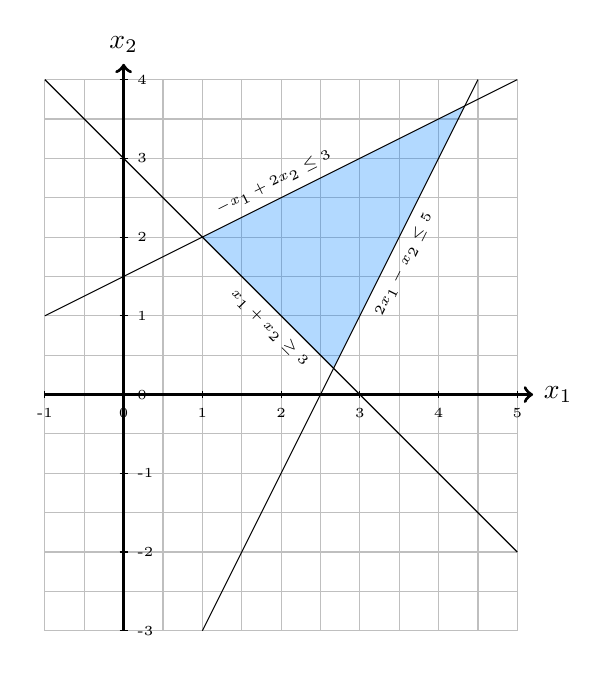
\begin{tikzpicture}

    \draw[gray!50, thin, step=0.5] (-1,-3) grid (5,4);
    \draw[very thick,->] (-1,0) -- (5.2,0) node[right] {$x_1$};
    \draw[very thick,->] (0,-3) -- (0,4.2) node[above] {$x_2$};

    \foreach \x in {-1,...,5} \draw (\x,0.05) -- (\x,-0.05) node[below] {\tiny\x};
    \foreach \y in {-3,...,4} \draw (-0.05,\y) -- (0.05,\y) node[right] {\tiny\y};

    \fill[blue!50!cyan,opacity=0.3] (8/3,1/3) -- (1,2) -- (13/3,11/3) -- cycle;

    \draw (-1,4) -- node[below,sloped] {\tiny$x_1+x_2\geq3$} (5,-2);
    \draw (1,-3) -- (3,1) -- node[below left,sloped] {\tiny$2x_1-x_2\leq5$} (4.5,4);
    \draw (-1,1) -- node[above,sloped] {\tiny$-x_1+2x_2\leq3$} (5,4);

	\end{tikzpicture}
	\end{center}
	
	\subsection{Remarkable Identities}\label{calculus remarkable identities}
	The remarkable identities are some kind of magical relations that we use most often for factoring or solving algebraic equations in all fields relative to Applied Mathematics. They have an important place and must be absolutely be mastered by the reader.
	
	Let us recall some notions that have already study in the section of Set Theory and of the chapter Arithmetic (we assume the concept of neutral element known as already defined):
	\begin{itemize}
		\item Commutativity:
		
		
		\item Associativity:
		
		
		\item Distributivity:
		
	\end{itemize}
	Similar properties are valid with the subtraction operation of course with the adequate domain of definition.
	
	\pagebreak
	We can check with numerical values (by replacing each abstract number a randomly chosen number), or by development (it would be better, so you are sure you have understood what we were talking about until now), that the following algebraic identities are satisfied (they are the most known one):
	\begin{enumerate}
		\item Second degree identity:
		
		\item Third degree identity:
		
	\end{enumerate}
	\begin{tcolorbox}[title=Remark,colframe=black,arc=10pt]
	We can very well put that in practice that $(a+(c+d))^2:=(a+b)^2$ where we obviously putted that $b:=c+d$ (we do an "abstract of the abstraction" or more commonly: a "change of variable"). And therefore:
	
	\end{tcolorbox}
	We can thus notice that in generality, to calculate the development $(a+b)^n$, we use the development of $(a+b)^{n-1}$, that is to say with the identity calculated with the previous value of $n$.
	
	We can also see a pattern if we put all together:
	
	We thus notice the following properties for $a$ and $b$:
	\begin{enumerate}
		\item The powers of $a$ decreasing from $n$ to $0$ ($a^0=1$, so it is not noted in the last term).
		
		\item The powers of $b$ increase from $0$ to $n$ ($a^0=1$, so it is not noted in the first term).
		
		\item In each term, the sum of the powers of $a$ and $b$ is equal to $n$.
		
		\item The multiplier coefficients in front of each term are calculated by summing the multipliers of two terms of development achieved with the previous value of $n$ (see figure below).
	\end{enumerate}
	The so named "\NewTerm{binomial coefficients}\index{binomial coefficient}" can then be obtained by the construction of the "\NewTerm{Pascal's triangle}\index{Pascal's triangle}\label{Pascal's triangle}" below:
	\begin{figure}[H]
		\centering
		\includegraphics{img/algebra/pascal_triangle.jpg}
		\caption{Pascal Triangle}
	\end{figure}
	Where each element is given by (\SeeChapter{see chapter Probability}):
	
	with $n,p\in \mathbb{N}^{+}$.
	\begin{theorem}
	We can then prove that\label{binomial theorem}
	
	which is the famous "\NewTerm{Newton's binomial}\index{Newton's binomial}" (that we will reuse many times in different chapters and thus sections of this book) or also named "\NewTerm{Binomial theorem}\index{binomial theorem}".
	
	More explicitly\label{binomial coefficient development}:
	
	also named "\NewTerm{binomial series}\index{binomial series}".
	\end{theorem}
	\begin{dem}
	This relation can be proved quite simply by induction assuming true the previous relation and calculating it for the rank $1$:
	
	This relation can be simply proved by induction assuming true the previous relation and for calculating for the rank $1$:
	
	The relation is true for rank $n + 1$, so it is true for any $n$.
	\begin{flushright}
		$\square$  Q.E.D.
	\end{flushright}
	\end{dem} 
	Regarding remarkable identities with negative values, there is no need to memorize the location of the sign "$-$". Just make a change of variable and once the development is made we replace the variable back (inverse change of variable).
	\begin{tcolorbox}[colframe=black,colback=white,sharp corners]
	\textbf{{\Large \ding{45}}Example:}\\
	
	and so on for all finite power $n$.
	\end{tcolorbox}
	We can of course mix genders (...) such as (particularly famous example):
	
	and some remarkable additional practical relation that are often used in small classes for exercises:
	
	\begin{tcolorbox}[title=Remark,colframe=black,arc=10pt]
	When, from the right-hand side (in a simplified numerical form) the teacher asks his students as an exercise to get the factoring of the left of the equality, there is no other way but to proceed by successive tests.
	\end{tcolorbox}
	For information we also get following famous development that is immediately deducible from what we have seen before:
	
	which is valid for any value of $b$ and is named the "\NewTerm{binomial expansion}\index{binomial expansion}". 
	
	For small $b$ we could neglect all terms involving $b^2$ or higher power of $b$, giving us the approximation relation:
	
	of $b\ll 1$.
	
	Of course there is still a lot of more useful relations with monomial (from which the biggest part is only a generalization of those presented above) that the reader will discover by his own reasoning and according to his practice and in this book through the different chapters.
	\begin{tcolorbox}[title=Remark,colframe=black,arc=10pt]
	It is of course possible to multiply polynomials between them and distribute the multiplicative terms. Conversely, it is often asked to students in small classes to do the reverse procedure ("factoring" or "decompose" a polynomial) so they get used to the handling of remarkable identities. Decomposed into a product of factors is an important operation in mathematics, since it is thus possible to reduce the study of complicated expressions to the study of several simpler expressions having interesting properties depending on the context.
	\end{tcolorbox}
	
	\subsection{Polynomials}\label{polynomial}
	\textbf{Definition (naive version \#\mydef):} We name "\NewTerm{algebraic univariate polynomial $P (x)$}\index{algebraic univariate polynomial}" a function of degree $n\in \mathbb{N}$ which is written:
	
	or in a more condensed manner by:
	
	 where the "\NewTerm{dominant factor}\index{dominant factor}" of a polynomial, also named "\NewTerm{leading coefficient}\index{dominant factor}", is the coefficient of the monomial of highest degree $a_n$ and the "\NewTerm{leading term}\index{leading term}" is simply $a_nx^n$.
	If we consider each coefficient of the polynomial as the component of a vector\label{polynomial vector}, then we can manipulate polynomials of degree less than or equal to as a vector space denoted $\mathcal{P}_n(\mathbb{R})$ and of dimension $n+1$.
	\begin{tcolorbox}[title=Remarks,colframe=black,arc=10pt]
	\textbf{R1.} The subscript $n$ of $P (x)$ is most of time omitted as explicitly defined in the expression.\\
	
	\textbf{R2.} The reader who has read the section of Set Theory, probably remember that the set of all polynomial of degree $n$ or lower form a vector space structure!
	\end{tcolorbox}
	\textbf{Definition (set theory version \#\mydef):} Let $k$ be a ring (\SeeChapter{see section Set Theory page \pageref{ring}}) and $n\in \mathbb{N}^{*}$, the "\NewTerm{polynomial ring}\index{polynomial ring}\label{polynomial ring}" in $n$ indeterminate (or variables) $k[X_1,...,X_n]$ is constructed from an elementary polynomial, named "\NewTerm{monomial}\index{monomial}" of the form:
	
	where $\lambda \in k$ is the "\NewTerm{coefficient of the monomial}\index{coefficient of the monomial}", $m_1,m_2,...,m_n$ are positive non-null integers and where $X_1^{m_1}...X_m^{m_n}$ forms the "\NewTerm{literal part of the monomial}\index{literal part of a monomial}". Thus, by construction, a polynomial is a sum of a finite number of monomials named the "\NewTerm{terms of the polynomial}\index{terms of a polynomial}".
	
	Therefore, the common special case used in small classes and presented at the beginning is $k[X]$, that is to say the ring of univariate polynomials with coefficients in $k$. Indeed most of time engineers and students deals with "ring of univariate polynomials with coefficient in $\mathbb{R}$" and denoted by $\mathbb{R}[X]$. Any element of $k[X]$ is therefore written as:
	
	with $a_i\in k$ (most of time  $a_i\in \mathbb{R}$ ), $i=0...n$ and $n\in \mathbb{N}$.
	\begin{tcolorbox}[title=Remarks,colframe=black,arc=10pt]
	\textbf{R1.} Notice that the powers $i$ are always positive or null in $k[X]$!!!\\
	
	\textbf{R2.} We say that two polynomials are "similar" if they have the same literal part.
	\end{tcolorbox}
	\begin{figure}[H]
		\centering
		\includegraphics{img/algebra/polynomials.jpg}
		\caption[Some polynomials plotted with R.3.2.1]{Some polynomials plotted with R.3.2.1 (see my book on R)}
	\end{figure}
	The "\NewTerm{limiting behavior}\index{limiting behavior}" of a function describes what happens to the function as $x\rightarrow \pm\infty$. The degree of a polynomial and the sign of its leading coefficient dictates its limiting behavior. In particular:
	\begin{itemize}
		\item If the degree of a polynomial $f(x)$ is even and the leading coefficient is positive, then $f(x)\rightarrow +\infty$ as $x\rightarrow \pm\infty$.
		\item If $f(x)$ is an even degree polynomial with negative leading coefficient, then $f(x)\rightarrow -\infty$ as $x\rightarrow \pm\infty$. 
		\item If $f(x)$ is an odd degree polynomial with positive leading coefficient, then $f(x)\rightarrow -\infty$ as $x\rightarrow +\infty$ and $f(x)\rightarrow +\infty$ as $x\rightarrow +\infty$.
 
		\item If $f(x)$ is an odd degree polynomial with negative leading coefficient, then $f(x)\rightarrow +\infty$ as $x\rightarrow -\infty$ and $f(x)\rightarrow -\infty$ as $x\rightarrow +\infty$.
	\end{itemize}
	These results are summarized in the table below.
	
	\begin{table}[H]
		\centering
		\begin{tabular}{|l|c|c|}
		\hline
		\rowcolor[HTML]{C0C0C0} 
		\textbf{Degree of the polynomial}     & \multicolumn{2}{l|}{\cellcolor[HTML]{C0C0C0}Leading coefficient}                                                                                                                                                                                                                                      \\ \hline
		                                      & $+$                                                                                                                                               & $-$                                                                                                                                               \\ \hline
		\cellcolor[HTML]{C0C0C0}\textbf{Even} & $f(x)\rightarrow +\infty$  as $x\rightarrow \pm\infty$                                                                                            & $f(x)\rightarrow -\infty$ as $x\rightarrow \pm\infty$                                                                                             \\ \hline
		\cellcolor[HTML]{C0C0C0}\textbf{Odd}  & \begin{tabular}[c]{@{}c@{}}$f(x)\rightarrow -\infty$ as $x\rightarrow -\infty$\\ $f(x)\rightarrow -\infty$ as $x\rightarrow -\infty$\end{tabular} & \begin{tabular}[c]{@{}c@{}}$f(x)\rightarrow +\infty$ as $x\rightarrow -\infty$\\ $f(x)\rightarrow -\infty$ as $x\rightarrow +\infty$\end{tabular} \\ \hline
		\end{tabular}
		\caption{Limiting Behavior of Polynomials}
	\end{table}
	\textbf{Definition (\#\mydef):} We name "\NewTerm{turning point}\index{turning point}" a point at which the graph changes direction from increasing to decreasing or decreasing to increasing (or differently said: where the derivatives is equal to zero).
	\begin{figure}[H]
		\centering
		\includegraphics[scale=0.5]{img/algebra/turning_points.jpg}
		\caption{Turning point explicitly highlighted}
	\end{figure}
	The function $f$ above is a $4^{\text{th}}$ degree polynomial and has $3$ turning points. The maximum number of turning points of a polynomial function is always one less than the degree of the function.
	
	\textbf{Definition (\#\mydef):} We name "\NewTerm{root}\index{root of a polynomial}" or "\NewTerm{zero of (univariate) polynomial}\index{zero of a univariate polynomial}", the $x$ values such as the "\NewTerm{polynomial equation}\index{polynomial equation}" $P(x)=0$ is satisfied at the condition that at least one of the $a_n$ with $n>0$ is not null.
	
	If the polynomial admits one or more roots $r_n$ we can then obviously factorize it as (we will prove it more rigorously further below):
	
	so that when $x$ takes the value of one of the roots $r_n$, the expression above is zero. This is what we name by convention "\NewTerm{factorize a polynomial}\index{factorize a polynomial}".
	
	Algebraic identities are particular forms of polynomial functions. Indeed, consider a constant $c$ and a variable $x$ and:
	
	We see that if we put:
	
	we fall back on:
	
	\textbf{Definitions (\#\mydef):}
	\begin{enumerate}
		\item[D1.] A polynomial in one indeterminate is named an "\NewTerm{univariate polynomial}\index{univariate polynomial}", a polynomial in more than one indeterminate is named a "\NewTerm{multivariate polynomial}\index{multivariate polynomial}". A polynomial with two indeterminates is named a "\NewTerm{bivariate polynomial}\index{bivariate polynomial}".
		
		A famous example in pure mathematics of a multivariate polynomial given many times in undergraduates course is: 
		
	
		\item[D2.] In the case of polynomials in more than one indeterminate, a polynomial is named  "\NewTerm{homogeneous of degree $n$}\index{homogeneous polynomial of degree $n$} if all its non-zero terms have degree $n$ (the example just above is such a polynomial!).
	\end{enumerate}
	
	\pagebreak
	\subsubsection{Euclidean Division of Polynomials}\label{polynomials division}
	Let us put ourselves now in the ring $k[X]$. If $P(x)\in k[X]$, we denote by $\text{deg}(P)$ the degree of the polynomial $P(X)$ with coefficients in a ring $k$ (real or complex ... whatever!)
	\begin{tcolorbox}[title=Remark,colframe=black,arc=10pt]
	By convention:
	
	\end{tcolorbox}
	\begin{theorem}
	Given:
	
	with $k,m>0$. Then there are two unique polynomial $q(X),r(X)\in k[X]$ such as:
	
	and:
	
	where $q(X)$ is the "\NewTerm{quotient polynomial}\index{quotient polynomial}" and $r(X)$ the "\NewTerm{residual polynomial}\index{residual polynomial}".
	\end{theorem}
	\begin{dem}
	If $u (X) = 0$ the result is obvious. Let us suppose that $u(X)\neq 0$ and let us prove the existence by induction on the degree $k$ of $u (X)$.
	
	If $k = 0$ then $q (X) = 0$ (since $m>0$) and therefore $r (X) = u (X)$ will do the job.
	
	Now let us suppose the statement for any $k\leq n$... (this supposition is completely free of charge...):
	
	Let $u (X)$ be of degree $k=n1$. If $m>n+1$ then $q (X) = 0$ and $r (X) = u (X)$ can also do the job.
	
	Otherwise, if $m\leq n+1$then by writing ($u_{n+1}$ is the $n+1$-th coefficient of the polynomial $u(X)$ and $v_m$ the $m$-th coefficient of $v(X)$:
	
	we reduce then $ u (X) $ to a polynomial of degree $ \ leq n $ since $v (X)$ is of degree $m$ (and that it exists)!
	
	Indeed, the term:
	
	removed (at least) the term of highest degree $u_{n+1}X^{n+1}$.
	
	By the induction hypothesis, there are $f(X)$ and $g(X)$ such as:
	
	with $\text{deg}(g)<m$. So after rearranging:
	
	and therefore:
	
	do the job!
	
	So by induction we see that the Euclidean division exists in the polynomial ring $k[X]$.
	\begin{flushright}
		$\square$  Q.E.D.
	\end{flushright}
	\end{dem}
	\begin{tcolorbox}[title=Remark,colframe=black,arc=10pt]
	This proved allowed us in the section of Set Theory to show that this ring is "principal".
	\end{tcolorbox}
	\begin{tcolorbox}[colframe=black,colback=white,sharp corners]
	\textbf{{\Large \ding{45}}Example:}\\\\
	We will seel only one example as the idea is always same. We want to divide $x^3+x^2$ by $x-1$ we get:
	\begin{equation}
		\renewcommand{\arraystretch}{1.2}
		\renewcommand{\arraycolsep}{2pt}
		  \begin{array}{rrrr|rrr}
		 x^3&+x^2 &   &\cdot(-1)&x  &-1 &  \\
		\cline{5-7}
		-x^3&+x^2 &   &  &x^2&+2x&+2\\
		\cline{1-2}
		    &2x^2 &   &  &   &   &  \\
		    &-2x^2&+2x&  &   &   &  \\
		    \cline{2-3}
		    &     &2x &  &   &   &  \\
		    &     &-2x&+2&   &   &  \\
		              \cline{3-4}
		    &     &   &+1&   &   &  \\ 
		  \end{array}
	\end{equation}	
	\end{tcolorbox}
	
	
	\pagebreak
	\subsubsection{Factorization Theorem of Polynomials}\label{factorization theorem}
	We will now prove an important theorem that is in fact originally illustrated (among others) by the remarkable identities we saw above:
	
	\begin{theorem}
	If a polynomial $P(X)\in k[K]$ with coefficients in $k$ of degree $n\geq 1$ has a root $x=r$ in the ring $k$, then we can factorize $P(x)$ by $(x - r)$ such that:
	
	where $Q$ is a polynomial of degree $n-1$ (and therefore can be a simple monomial).
	
	In other words, "\NewTerm{factorize a polynomial}\index{factorization of polynomial}", it is written it as a product of monomials (in the general case: of polynomial). When not only applied to polynomials or also simply to numbers, factorization is an operation that transforms a sum into a product!
	\end{theorem}
	\begin{dem}
	The idea is to perform the Euclidean division of $P(x)$ by $(x-r)$. According to the previous theorem, there exists a pair $(Q, R)$ of polynomials such as:
	
and according to the result of the previous theorem on the Euclidean division:
	
	But $\text{deg}(x-r)=1$, so $\text{deg}(R)=0$ (or $-\infty$ by convention). $R(x)$ is therefore a constant polynomial function. Moreover, by hypothesis, $r$ is a root of $P(x)$. We have therefore:
	
	So $R(r)=$. Therefore $R(x)$ is the zero polynomial and the theorem is practically proved. It remains to prove that $\text{deg}(Q)=n-1$, which is an immediate consequence of the relation:
	
	Hence:
	
	\begin{flushright}
		$\square$  Q.E.D.
	\end{flushright}
	\end{dem}
	From this property to factorize a polynomial, named sometimes "\NewTerm{factorization theorem}\index{factorization theorem}", we can give a foretaste of a much more important theorem:
	\begin{theorem}
	Let us show that if we have a polynomial  function $P(X)\in k[X]$ of degree $n\in \mathbb{N}$ with coefficients in $k$, then it has at most a finite number $n$ of roots (some being possibly confused) in $k$.
	\end{theorem}

	\begin{dem}
	First, because $P(x)$ has a degree (order), $P(x)$ is not a zero polynomial function. Then, let us argue by the absurd:
	
	If the function $P(x)$ has $n$ roots with $p>n$ (more roots than degree....), by noting these roots $r_1,...,r_p$, we have, by the previous  factorization theorem (applied $p$ times):
	
	where $Q$ is a polynomial of degree:
	
	Now, since by definition a polynomial is a polynomial if and only if its degree (order) belongs to  $\mathbb{N}$, the polynomial $Q$ must be the zero polynomial such that:
	
	It follows that:
	
	This contradicts the initial hypothesis that $P$ is not the zero polynomial, hence:
	
	\begin{flushright}
		$\square$  Q.E.D.
	\end{flushright}
	\end{dem}
	
	\subsubsection{Diophantine equation}\label{diophantine equation}
	If we generalize the concept of univariate polynomial with several variables such as:
	
	then we name "\NewTerm{Diophantine equation}\index{Diophantine equation}" an equation of the form:
	
	where $P$ is a polynomial with integer (or rational) coefficients for which seeks the radicals (roots) strictly in $\mathbb{N}$ or $\mathbb{Q}$. Conventional Diophantine equations are for examples:
	\begin{itemize}
		\item  The linear Diophantine equations:
		
		
		\item The Pythagorean triples:
			
	\end{itemize}
	For the general proof of the latter, the reader will have to wait a little bit the time for the as authors of this book to have time understand to understand the proof (...).
	
	\subsubsection{First order univariate Polynomial and Equations}
	Given the linear function:
	
	If $a\neq 0$ the this first the equation:
	
	has a simple closed formed root given obviously by:
	
	such that $P_1(r)=0$.
	If $b=0$ this polynomial is named an "\NewTerm{affine function}\index{affine function}".
	
	\begin{tcolorbox}[title=Remarks,colframe=black,arc=10pt]
	\textbf{R1.} If the coefficients of the univariate polynomial of defree $1$ are all such that  $a,b\in \mathbb{R}$ then the root also belongs to $\mathbb{R}$.\\
	
	\textbf{R2.} If one of coefficients of the univariate polynomial of defree $1$ belongs to $\mathbb{C}$ then the root also belongs to $\mathbb{C}$.\\
	
	\textbf{R3.} If the both coefficients of the univariate polynomial of defree $1$ belongs to $\mathbb{C}$ then the root also belongs to $\mathbb{C}$ or $\mathbb{R}$.\\
	
	\textbf{R4.} We say that two polynomial equations are "\NewTerm{equivalent}\index{equivalent polynomials}" if the admit the same solutions.
	\end{tcolorbox}
	Here are also some properties for univariate first order polynomials that we give without proof as they seem very very intuitive to us (except on reader request):
	\begin{enumerate}
		\item[P1.] If we add (or respectively subtract) a same number to each member of the question (left from the "$=$" sign, and also right), we get an equation that has the same solutions as the original equation (and this whatever is its degree).
	
		\item[P2.] If we multiply (or respectively divide) each me member of an equation (left from the "$=$" sign, and also right) by a same non-null number, we get an equation that has the same solutions as the original equation (and this whatever is its degree).
	\end{enumerate}
	The method should be general enough to by applied to all equations of the same kind, be build on the four arithmetic basis operations (addition, subtraction, multiplication and division) and the extraction of roots. We we can find the solutions (roots), of an equation thanks to its coefficients, using only the previous operations (that is to say in a "\NewTerm{closed form}\index{closed form}"), we then say that the equation can be solved by "\NewTerm{radicals}\index{radicals}".
	
	\paragraph{Solving by circular reference}\mbox{}\\\\
	Many executives in the small, medium and international companies no longer know how to solve linear equations of the first degree (and beyond also of course...). So I think i the be interesting to the student of see how the hug majority of the people that are not able to solve such high-school level problems proceed (it's especially interesting when you know that they are paid quite a lot to solve such "complicated" problem according to their board committee) The easiest way to see this is how I see they use the spreadsheet software Microsoft Excel. Indeed, consider the following example:

	A company makes a turnover (income) of $1,500$.- and has to pay $1,000$.- of fixed costs (costs). It has $40\%$ tax payable after deduction. The company would like to make a donation (tax deductible) such that the amount of this donation represents $10\%$ of taxes after deduction.

	This is written mathematically simply if we denote by $R$ the turnover, $C$ the fixed costs, $D$ the donation, $t$ the tax rate:
	
	
	After some small trivial rearrangements we get:
	
	This corresponds well to the $10\%$ tax after deduction since:
	
	
	And here's how (bad) executives using a spreadsheet like Microsoft Excel and "solve" this (you can trust me I really see people do this in corporation because they are not able to solve problem on the paper anymore). First they write in the spreadsheet software (which automatically detects the inconsistency of the user by indicating it with a blue arrow to highlight the "circular reference"):
	\begin{figure}[H]
		\centering
		\includegraphics{img/algebra/circular_reference_microsoft_excel_01.jpg}
		\caption{Solving simple equation by circular reference in Microsoft Excel}
	\end{figure}
	Validated this gives:
	\begin{figure}[H]
		\centering
		\includegraphics{img/algebra/circular_reference_microsoft_excel_02.jpg}
	\end{figure}
	To solve this equation, it is necessary to activate in the software options the authorization to use the iteration (the position of this option depends on the version of the spreadsheet). 
	\begin{figure}[H]
		\centering
		\includegraphics[scale=0.8]{img/algebra/circular_reference_microsoft_excel_03.jpg}
		\caption[]{Recurring equation solving option in Microsoft Excel 14.0.7183}
	\end{figure}
	Which then gives:
	\begin{figure}[H]
		\centering
		\includegraphics{img/algebra/circular_reference_microsoft_excel_04.jpg}
	\end{figure}
	So as wee can see, this is quite a non-efficient way to solve a simple high-school problem (a shame for managers or business analysts that have MBA...!).

	\subsubsection{Second order univariate Polynomial and Equations}\label{second order polynomials}
	Given the following univariate polynomial with coefficient in $\mathbb{R}$ (trinomial of second degree):
	
	If we represent this univariate polynomial on the plane, this give us:
	\begin{figure}[H]
		\centering
		\includegraphics{img/algebra/polynomial_orientation.jpg}
		\caption{Typical orientation for second degree polynomials}
	\end{figure}
	If we take the derivative of this function (\SeeChapter{see section Differential and Integral Calculus page \pageref{differential calculus}}) and we search in what point the derivative is equal to zero, we will always found the optimum on the inflection point (\SeeChapter{see section Differential and Integral Calculus page \pageref{inflection point}}) of the parabola (which corresponds also to its symmetry axis):
	\begin{figure}[H]
		\centering
		\includegraphics{img/algebra/polynomial_optimum.jpg}
		\caption{Inflection point of the tangent?}
	\end{figure}
	If $a\neq 0$, then we have:
	
	We then have a "\NewTerm{double root}\index{double root}\label{double root}" (or "\NewTerm{root of multiplicity $2$}") that we denote by:
	
	such that $P(r_{1,2})=0$ and we define a new term named sometimes the "\NewTerm{determinant of the polynomial}" and most commonly the "\NewTerm{discriminant of the polynomial}\index{discriminant of the polynomial}\label{discriminant}":
		
	Finally\label{second order polynomial roots}
	
	If the second order univariate polynomial on $x$ has two root, we can then factorize it in an irreductible form (following the factorization theorem proved earlier) in the following form:
	
	We also prove easily from the expression of the root by doing simple algebra the "\NewTerm{Vieta relations}\index{Vieta relations}\label{vieta relations}" (on request of the readers we can detail the developments in necessary):
	
	
	Depending on the sign of $2a$ and this of the discriminant $\Delta$, we have:
	\begin{figure}[H]
		\centering
		\includegraphics{img/algebra/polynomial_second_order_signature.jpg}
	\end{figure}
	Therefore:
	\begin{itemize}
		\item If $\Delta<0$ our polynomial has no real roots and cannot be factorized in a multiplication of monomial with real ($
\mathbb{R}$) factor but with complex one ($\mathbb{C}$). Therefore (it is recommended to have read first the part about Complex Numbers in the section Numbers of this book):
		
		and we know that we can write any complex number in a condensed form (Euler formula) and as the complex roots of a polynomial of the second degree are conjugate (we already know this jargon) we have:
		
		where (recall) $r$ is the module of the complex roots (module that is equal for the both) and $\varphi$ the argument of the complex roots (equal in absolute value).
		
		\item If $\Delta=0$ the polynomial equation then has a single solution that is obviously:
		
		
		\item If $\Delta>0$ the polynomial equation then has two solutions defined by the general relations which we have already given above:
		
	\end{itemize}
	About the complex case, let us take as an example the following quadratic polynomial:
	
	that admits only two complex roots that are $\mathrm{i}$ and $-\mathrm{i}$. In the real plane this polynomial will be represented with Maple 4.00b by:
	
	\texttt{>plot(x\string^2+1,x=-5..5);}
	\begin{figure}[H]
		\centering
		\includegraphics{img/algebra/polynomial_complex_solutions_in_real_plane.jpg}
		\caption[]{Plot example of a polynomial of degree $2$ which admits only complex solutions}
	\end{figure}
	where we see well that there is no real solutions (zeros). While  placing us in the complex $\mathbb{C}$, we have:
	
	\texttt{>plot3d(abs((re+I*im)\string^2+1),re=-2..2,im=0..2,view=[-2..2,-2..2,0..2],\\
	orientation=[-130,70],contours=50,style=PATCHCONTOUR,axes=frame,\\
	grid=[100,100],numpoints=10000);}
	\begin{figure}[H]
		\centering
		\includegraphics{img/algebra/polynomial_complex_solutions_in_complex_plane.jpg}
		\caption[]{The same polynomial but playing with the complex representation}
	\end{figure}
	where the two zeros are visible on the imaginary axis at $-1$ and $+1$. Obviously when it's the first time we see a function shown in a figure taking into account the complex values we try to find where is the corresponding parabola of the purely real case. To do this, we simply cut the surface above on two on the imaginary axis and we get then:
	
	\texttt{>plot3d(abs((re+I*im)\string^2+1),re=-2..2,im=0..2,view=[-2..2,-2..2,0..2],\\
	orientation=[-130,70],contours=50,style=PATCHCONTOUR,axes=frame,\\
	grid=[100,100],numpoints=10000);}
	\begin{figure}[H]
		\centering
		\includegraphics{img/algebra/polynomial_complex_solutions_in_complex_plane_cutted.jpg}
		\caption[]{A little zoom on the same polynomial}
	\end{figure}
	where we find again clearly our parabola visible on the cutted surface. So we can ask ourselves whether the complex numbers are a natural extension of our conventional space beyond our physical senses and our common measuring devices...!

	\paragraph{Irrational Equations}\mbox{}\\\\
	The practitioner must always take the habit to verify the solution in the original equation to be sure of the validation of the definition domain of the function. Indeed, there are solutions to the resolution of equations that do not satisfy the original equation and this is what we name "\NewTerm{extraneous solutions}\index{polynomial extraneous solution}" and this is typically the case of irrational equations. 

	\textbf{Definition  (\#\mydef):} An "\NewTerm{irrational equation}\index{irrational equation}" is an equation where the unknown is under a radical (that is to say in typical case: under a square root).
	
	\begin{tcolorbox}[colframe=black,colback=white,sharp corners]
	\textbf{{\Large \ding{45}}Example:}\\\\
	Consider the following equation
	
	To solve it first we can redistribute:
	
	With take the power of $2$:
	
	We simplify little bit:
	
	again:
	
	We take the power of $2$ again:
	
	We simplify a last time:
	
	We get two trivial solution that are $x_1=-2$ and $x_2=2$. But only the solution $x_1=-2$ satisfy the proposed equation. Indeed, if you put the first solution in the original equation we get:
	
	But if we put the second one:
		
	\end{tcolorbox}
	
	\pagebreak
	\paragraph{Gold Number}\mbox{}\\\\
	There is a second order univariate polynomial whose solution is famous around the world. The solution is a value named the "\NewTerm{golden ratio}\index{golden ratio}" or "\NewTerm{Divine proportion}\index{divine proportion}" (...) and is found in architectural, aesthetic or in phyllotaxis (that is to say, in the arrangement of the leaves around the stem of the plants).
	
	This number is:
	
	The golden ratio is also an algebraic number (any complex number that is a root of a non-zero polynomial in one variable with rational coefficients) and even an algebraic integer (complex number that is a root of some monic polynomial with coefficients in $\mathbb{Z}$) as it is solution of:
	
	There is a very elegant way to bring out this polynomial of using the $\mathcal{Z}$ transform and that we will discuss in the section of Functional Analysis.
	
	\subsubsection{Third order univariate Polynomial and Equations}
	Even if rare to solve in theoretical physics or in engineering, solving an univariate polynomial of the $3$rd degree is quite recreational and shows a good example of an already mature mathematical reasoning (we have these developments thanks Scipione del Ferro and Jerome Cardan mathematicians of the 16th century...).
	
	Given the equation:
	
	with the coefficients in $\mathbb{R}$ (to begin...). In a first time, the reader will be able to see that the reasoning that we have applied for the polynomial a smaller order than $3$ stuck when the order is greater (excepted for special simple cases obviously...).

	We will avoid the problem by using a change of variables subtle but quite justified.
	
	Thus, nothing prevents us from putting that:
	
	and that by dividing the polynomial of degree 3 by $a$ to write:
	
	By grouping the terms of the same order:
	
	and let us write (nothing, but really nothing prevent us to do this):
	
	where (1) est known if and only if $X$ is known and where $p,q$ are anyway unknowns.

	The polynomial\footnote{The first time a had to solve such a polynomial was to calculate the nutation of a gyroscope and the second time was for the calculation of the horizon of a Black Hole based on the Schwarzschild metric with cosmological constant that was in natural units: $\dfrac{\Lambda}{3}r^3-r-2M=0$}:
	
	being of odd degree, it admits (as it can be seen from any visual plot of such a polynomial with real coefficients) at least one real root, named the "\NewTerm{certain root}\index{certain root}" and at maximum three roots. The reader will easily check by himself that with a graphical representation of an odd degree polynomial this is trivial!
	
	Now let us make another subtle change of variable (we have the right to do this):
	
	by imposing the condition that $u, v$ must be such that $3uv=-p$ (nothing prevents us from imposing such a constraint), then we have:
	
	Therefore we have:
	
	We can very well make an analogy between the two equations (1') and (2') and the Vieta relations we had obtained for the polynomial of degree 2 which we recall were:
	
	excepted that we have now (we adopt another notation for these intermediate roots):
	
	which gives us for the polynomial $P$ by imposing (always by analogy) $a=1$ a new equation:
	
	for which $z_1,z_2$ are the roots.
	The latter equation has for discriminant:
	
	Let us take now scenario by scenario:
	\begin{enumerate}
		\item If $\Delta >0$, the equation on $Z$ admits two solutions $z_1,z_2$ whose sum will give us indirectly the value of $X$ since by definition $X=u+v$ and $z_1=u^3$ and $z_2=v^3$. We see that we have all the ingredients to find the first root of the original equation that will be the certain root (or "\NewTerm{certain zero}\index{certain zero}"). So:
		
		as $\Delta>0$ and the superior roots are cubic we necessarily have $X_1\in \mathbb{R}$ if all coefficient of the equation are well in $\mathbb{R}$.
		
		\item If $\Delta=0$, we know it, the equation on $Z$ admit a double root and as the discriminant has a square power of $q$ this means necessarily that $p$ is negative.

		The polynomial $P$ therefore also has a double root and the same for the original equation. We saw also that for a second degree polynomial if the discriminant is zero roots are:
		
		Then by analogy:
		
		
		\item If $\Delta<0$ we must again use complex numbers as we did in our study of the polynomial of degree $2$. Thus, we know that the equation $Z$ admits two complex solutions such as:
		
		and once again as the roots are conjugated we can write in condensed form:
		
		and as:
		
		we therefore have:
		
		As $u_k,v_k$ are conjugated, we have necessarly $X_k\in \mathbb{R}$.
	\end{enumerate}
	
	\pagebreak
	\begin{tcolorbox}[colframe=black,colback=white,sharp corners]
	\textbf{{\Large \ding{45}}Example:}\\\\
	Consider the following equation:
	
	We therefore have:
	
	and therefore:
	
	We therefore have:
	
	\end{tcolorbox}
	The polynomials of degree three are therefore well solvable by radicals.
	
	\subsubsection{Fourth order univariate Polynomial and Equations}
	The univariate polynomial equation to solve here is:
	
	with $a\neq 0$.
	\begin{tcolorbox}[title=Remark,colframe=black,arc=10pt]
	We own the method of resolution of $4$th degree polynomial to the Italian mathematician  Ludovico Ferrari (also) of the 16th century.
	\end{tcolorbox}
	If we divide by $a$ we have:
	
	And by putting:
	
	the equation will be reduce to:
	
	where we see that the coefficient in front of the $y^3$ vanishes. Thus, any polynomial of the type:
	
	can be written in the following form:
	
	By putting:
	
	\begin{tcolorbox}[title=Remark,colframe=black,arc=10pt]
	If $d''=0$ the equation to solve is reality a "\NewTerm{bisquare equation}\index{bisquare equation}". The change of variable $X=y^2$ then allows to focus to a polynomial equation of the second degree (what we know is easily to solve).
	\end{tcolorbox}
	We now introduce a parameter $t$ (that we will choose wisely afterwards) and we rewrite the polynomial equation as follows:
	
	\begin{tcolorbox}[title=Remark,colframe=black,arc=10pt]
	If the reader develop and distribute all the terme of the previous relation he will fall back obviously on $x^4+c''x^2+d''x+e''=0$.
	\end{tcolorbox}
	The underlying idea is to try to ensure that the bracketed part of the previous expression can be written as a square as:
	
	Because in this case, using:
	
	Our polynomial equation can then be written:
	
	and we would have only to solve two polynomial equations of the second degree (what we know already how to do).
	
	But for us to write:
	
	the expression of second degree to the left of equality should have only one root. But we saw in our study of polynomial equations of the second degree that meant since the discriminant is zero:
	
	and that the root was given by:
	
	Which corresponds in our case to:
	
	and therefore that:
	
	with:
	
	So finally, if $t$ is such that $4(2t-c'')(t^2-e'')={d''}^2$, then we have:
	
	as the fundamental polynomial theorem give us for a polynomial of the second degree a unique root:
	
	To conclude, it is enoughe to find a number $t$ satisfying the following relation:
	
	which is a degree $3$ polynomial that we already know how to solve using the Cardan method.

	Such general methods doesn't exist anymore for polynomial of degree higher or equal to $5$ as we will prove it during our study of Galois Theory (\SeeChapter{see section Set Algebra page \pageref{galois theory}}).
	
	\subsubsection{Trigonometric Polynomials}\label{trigonometric polynomials}
	\textbf{Definition (\#\mydef):} We name "\NewTerm{trigonometric polynomial of degree $N$}\index{trigonometric polynomial}" any finite sum of the type:
	
	where $c_n\in \mathbb{C}$.

	A trigonometric polynomial can also be written using the usual trigonometric functions with the following changes:
	
	Either using Euler's formula (\SeeChapter{see section Numbers page \pageref{euler formula}}):
	
	What we can also rewrite as:
	
	By putting:
	
	It comes:
	
	We will extensively discussed in the section Sequences and Series how to use these polynomials in the context of the study of Fourier series.
	
	\subsubsection{Cyclotomic Polynomials}
	If $n$ is an integer (belongs to $\mathbb{N}$) and $x$ a complex number (belongs to $\mathbb{C}$), we name "\NewTerm{cyclotomic polynomial}\index{cyclotomotic polynomial}" that we denote traditionally by $\Phi_n$ and that we define as being the product of all monomials:
	
	where $\alpha$ is a $n$th primitive root of $\mathbb{C}$. In other words:
	
	To recall an $n$th unit root (sometimes named "\NewTerm{De Moivre number}\index{De Moivre number}") is a complex number whose $n$-th power is equal to $1$.
	
	Thus, the set of all $n$-th unit roots is given by:
	
	which is a cyclic group (see the section Set Theory and also the section Set Algebra).

	Then we name "\NewTerm{$n$-th primitive root of unity}\index{primitive root of unity}" any element of this group generating it.
	
	The elements of $G_n$ are of the type:
	
	with $k\in \mathbb{Z}$. We write then the set of the $G_n$ in the form:
	
	A small example of cyclotomic polynomial (more example will be given below):
	
	with:
	
	which are therefore the $4$th roots of unity (in other words: each of these number set to the power of $4$ is equal to $1$). They form the group $G_4$ and this can be generated only by $\mathrm{i}$ and $-\mathrm{i}$ (field generator according to what was seen in the section Set Theory).
	
	So a cyclotomic polynomial is the product of factors that is written:
	
	with $k\in \{0,\ldots,n-1\}$.
	
	We will see with the examples below that if $n$ is even then:
	
	and if $n$ is odd:
	
	
	\pagebreak
	\begin{tcolorbox}[colframe=black,colback=white,sharp corners]
	\textbf{{\Large \ding{45}}Example:}\\\\
	For $n$ up to $30$, the cyclotomic polynomials are:
	
	\end{tcolorbox}
	
	\subsubsection{Legendre Polynomials}\label{legendre polynomials}
	\textbf{Definition (\#\mydef):} Legendre polynomials are define by (it is strongly recommended to read the sections of Differential and Integral Calculus and also of Functional Analysis before continuing):
	
	where $P_n$ is therefore a polynomial of degree $n$. We will see again these polynomials in the resolution of differential equations in physics (heat propagation, quantum physics, quantum chemistry, etc.). In most book the Legendre polynomial are written in the following equivalent form:
	
	We will focus here only and uniquely on the properties that will are used actually in the other physic sections of this book!!!
	
	Let us prove that following definition of functional scalar product (see the sections Functional Analysis and Calculation Vector) Legendre polynomials are orthogonal. This is a very important property for our study of Quantum Chemistry!
	
	\begin{dem}
	Let $P$ be a polynomial of degree $\leq n-1$. It suffices to prove that $\langle P_n | P \rangle =0$, that is to say that $P_n$ is orthogonal to the space of polynomials of degree less than $n$. Indeed, we have:
	
	integrating by parts we get:
	
	Caution!!! For the above zero term, only the term $(1-x^2)^n$ is derived there! So since $x$ is squared, whatever the derivative the value will always be the same. What justifies this term is equal to zero.
	
	Continuing in this way we get after $n$ integration by parts:
	
	\begin{tcolorbox}[title=Remark,colframe=black,arc=10pt]
	The derivative term is zero, since the derivative polynomial is of degree $n-1$.
	\end{tcolorbox}
	\begin{flushright}
		$\square$  Q.E.D.
	\end{flushright}
	\end{dem}	
	Here are some useful properties for the section of Quantum Chemistry of the Legendre polynomials:
	\begin{enumerate}
		\item[P1.] We have $P_n(1)=1$:
		\begin{dem}
		
		and using the Leibniz Formula (\SeeChapter{see section Differential and Integral Calculus page \pageref{leibniz formula}}) we have:
		
		Therefore:
		
		\begin{flushright}
			$\square$  Q.E.D.
		\end{flushright}
		\end{dem}

		\item[P2.] We have $P_n(-x)=P_n(-x)$ if $n$ is even:
		\begin{dem}
		If $n$ is even:
		
		is an even function and therefore:
		
		is even.
		\begin{flushright}
			$\square$  Q.E.D.
		\end{flushright}
		\end{dem}

		\item[P3.] We have $P_n(-x)=-P_n(x)$ if $n$ is odd:
		\begin{dem}
		If $n$ is odd:
		
		is an odd function and therefore:
		
		is odd.
		\begin{flushright}
			$\square$  Q.E.D.
		\end{flushright}
		\end{dem}
	\end{enumerate}
	\begin{theorem}
	We will now prove the validity of the following recurrence relation for the $P_n$ (relations that we use in physics):
	
	for $n \geq 1$.
	\end{theorem}
	\begin{dem}
	$xP_n(x)$ is a polynomial of degree $n+1$, there exists therefore $a_j\in \mathbb{R}$ such that this polynomial can be expressed as a linear combination of the family of polynomials constituting the orthonormal basis (basis that enables us to generate/build the $xP_n(x)$):
	
	Therefore we can write:
	
	but if we choose $k\leq n-2$ (because $xP_k$ is therefore of degree $n-1$):
	
	Therefore:
	
	that is to say that $a_k=0$. Than it follow:
	
	By the properties of the Legendre polynomials proved previously, we can write the equalities:
	
	and:
	
	hence:
	
	The dominant coefficient of $P_n$ denoted by $\text{dom}(P_n(x))$ is defined (for recall) as the coefficient of the monomial of the highest degree. Thus, it is given by:
	
	Therefore:
	
	\begin{tcolorbox}[title=Remark,colframe=black,arc=10pt]
	The reader will verify if needed for a given $n$ that:
	
	\end{tcolorbox}
	The relation:
	
	we got earlier impose us that the dominant coefficient of the polynomial of the linear combination to be equal to the dominant coefficient of the polynomial $xP_n$ (we have eliminated the $(-1)^n$ which simplifies):
	
	After simplification we get:
	
	and which finally gives easily:
	
	The relation:
	
	becomes therefore:
		
	\begin{flushright}
		$\square$  Q.E.D.
	\end{flushright}
	\end{dem}
	The first Legendre polynomials are:
	

	The graphs of these polynomials (up to $n = 5$) are shown below:
	\begin{figure}[H]
		\centering
		\includegraphics{img/algebra/legendre_polynomials.jpg}
		\caption[Five first Legendre Polynomials]{Five first Legendre Polynomials (source: Wikipedia)}
	\end{figure}
		

	\begin{flushright}
	\begin{tabular}{l c}
	\circled{90} & \pbox{20cm}{\score{3}{5} \\ {\tiny 70 votes,  56.29\%}} 
	\end{tabular} 
	\end{flushright}
	
	%to make section start on odd page
	\newpage
	\thispagestyle{empty}
	\mbox{}
	\section{Set Algebra}\label{set algebra}
	\lettrine[lines=4]{\color{BrickRed}W}e will approach in this book the study of set structures very pragmatically (since you must remember that this book is dedicated to engineers). Thus, it will be made use of the minimum of formalism and only the proofs of the elements that we consider as absolutely essential to the engineer will be presented in this. Moreover, numerous proofs will be made by example and we will focus largely on the algebraic theory of groups as it has a prominent place in physics almost more than for other set-structures.

	\subsection{Groups Algebra and Geometry}
	The symmetries of geometric figures, of crystals and all the other items of macroscopic physics, are subject for centuries of observations and studies. In modern terms, the symmetries of a given object form a "group".
	
	Since the mid-19th century, the group theory took a huge extension, and its applications to quantum mechanics and the theory of elementary particles have developed throughout the 20th century.
	
	In a letter of 1877 to the mathematician Adolf Meyer, Sophus Lie wrote that he created the theory of groups in January 1873. It is of the groups he named "\NewTerm{continuous groups}\index{continuous groups}" and that are named today "\NewTerm{Lie groups}\index{Lie groups}\label{lie group}". Lie sought to expand the use of groups from the domain of algebraic equations, where Galois had introduced them, to the differential equations.
	
	Since 1871, the notion of infinitesimal generator of a one-parameter group of transformations appeared in his work. This is the set of infinitesimal generators of the subgroups with one parameter of a continuous group that forms what we name today a "\NewTerm{Lie algebra}\index{Lie algebra}".
	
	It was Weyl and Wigner that show the preeminent role of the theory of groups and their representations in particular in the new quantum mechanics that Heisenberg  and Dirac were developing. The general idea of representation theory is try to study a group by doing it acting on a vector space in a linear way: we try to see the group as as a group of matrices (hence the term "representation "). We can, from relatively well-known properties of the automorphism group of the vector space (\SeeChapter{see section Set Theory page \pageref{automorphism}}), get to deduce some group properties of main interest.
	
	We can consider the theory of group representations as a vast generalization of the Fourier analysis. Its development is continuous and has, since the mid-20th century, countless applications in differential geometry, ergodic theory, probability theory, number theory, the theory of automorphic forms, in that of dynamic systems as well as in physics, chemistry, molecular biology and signal processing. Currently, entire branches of mathematics and physics depend on it.
	
	Before we begin, we refer the reader to the section on Set Theory to get a refresh of the structure and fundamental properties that make up a Group and also to the section of Linear Algebra (because we use some results proved in it).
	
	\subsubsection{Cyclic Groups}\label{cyclic groups}
	The cyclic group (whose definition of has already been given in the section of Set Theory) will serve us a basis for the study of finite groups. Moreover, rather than making generalized expansions we preferred to take specific examples to present the idea of cyclic group (more suitable for an engineering approach).
	
	We will take then the very nice example of the hours of a clock... with three different approaches that will successively (!) and simple address the concept of a cyclic group.
	\begin{enumerate}
		\item First approach:
		
		Let us imagine a clock with a needle which can take $12$ possible positions (but no intermediate positions). We will denote in a special way the $12$ possible positions: $\overline{0},\overline{1},\overline{2},...,\overline{11}$  (the line above the numbers is not innocent!).
		
		Nothing prevents us on all of these positions to define an addition, for example:
		
	  	which is similar to the results we get when we in our daily life we do calculations manipulating time.
	  	
	  	\item Second approach (first extension):
	  	
	  	If we observe well a Watch or a Clock, we notice that every time we add $12$ (or withdraw $12$...) to a value of hours of our Watch/Clock then we fall back on the set of numbers that are well defined that are also in $\mathbb{Z}$. Therefore (obviously as part of a Watch/Clock only the first positive values are of interest to us most of the time but here we do math so we generalize a bit...)
	  	
		Here we fall back on a concept we had already seen in the section of Numbers Theory. This are congruence classes and all of these classes form the quotient set $\mathbb{Z}/12\mathbb{Z}$. If we endow this quotient set of an addition law, it is normally easy to observe that it is an internal law to the quotient set, that it is associative, that there exist a neutral element and that every element has an inverse (opposite).
		
		Thus, this quotient set equipped only with the addition law (if adding the multiplication we can form a ring) is a commutative group.

		\item Third approach (second and last extension):
		
		Let us see a third and final approach which is why the quotient group is cyclic.
		
		If we project the rotation of the hands of our Watch/Clock (all rotations in the set-algebra are traditionally clockwise!) in $\mathbb{C}$ and that we define:
		
		We then have $x^{12}=x^0=1$ and:
		
		which is why the quotient group $(\mathbb{Z}/12\mathbb{Z},+)$ is named "\NewTerm{cyclic group}\index{cyclic group}" (by group isomorphism according to what has been seen in the section Set Theory). Its isomorphic is noted by $C_{12}$ and all elements are of modulus $1$. It is common to denote all complex number of modulus $1$ as following:
		
		If we represent in $\mathbb{C}$ the isomorphic set $C_{12}$ we get then on the unit circle a polygon with $n$ vertices as shown in the figure below:
		\begin{figure}[H]
			\centering
			\includegraphics{img/algebra/c_12_cyclic_group.jpg}
			\caption{$C_{12}$ Cyclic Group}
		\end{figure}
		Furthermore, the number of component elements of $\mathbb{Z}/12\mathbb{Z}$ being finite, $(\mathbb{Z}/12\mathbb{Z},+)$ is finite. Unlike the group $(\mathbb{Z},+)$ which is itself a discrete infinite group.
		
		This concept of finitude is perhaps most obvious with the example that we will do afterwards with $\mathbb{Z}/4\mathbb{Z}$ where the reader will observe that this set has the same number of elements than $C_4$.	
	\end{enumerate}
	
	\begin{tcolorbox}[title=Remark,colframe=black,arc=10pt]
	Mathematicians name $C_n$ the "group of $n$-th roots of unity". An $n$-th root of the unit (sometimes named "\NewTerm{De Moivre's number}\index{De Moivre's number}") is a complex number whose $n$-th power is equal to $1$. Moreover, for a given integer $n$, all $n$-th roots of unit are located on the unit circle and are the vertices of a regular $n$-sided polygon having an apex of affix $1$.
	\end{tcolorbox}
	
	\textbf{Definition (\#\mydef):} A "\NewTerm{finite group}\index{finite group}\label{finite group}" is a mathematical group with a finite number of elements like "permutations groups", "symmetric groups", "cyclic groups", etc.
	
	What interests particularly physicists at first are the representations of finite groups (also the continuous groups that we will see later). Thus, the representative of $\mathbb{Z}/n\mathbb{Z}$ is know to us as the rotation in the complex plane is given as we have shown during our study of complex numbers in the section Numbers:
	
	with $k\in[0,n-1]$. This representative is a subgroup of the group of rotations $\text{O}(2)$ which will be discussed further. The group of rotations of the plane itself being a subgroup of the linear group $\text{GL}(2)$ (we will give a precise definition and an example further below).
	
	In fact, mathematicians are able to prove that all quotients groups $\mathbb{Z}/n\mathbb{Z}$ are cyclic to an isomorphism with $C_n$ and then they say that $\mathbb{Z}/n\mathbb{Z}$ is a finite quotient of the monogenic group $\mathbb{Z}$...
	
	This approach is perhaps a bit abstract for the Padawan... So if the reader remembers the section Set Theory we saw a very precise definition of what is the cyclicity of a group: A group $G$ is said to cyclic if $G$ is generated by the power of at least one of its elements $a\in G$ named the "generator" such that:
	
	Let us check whether this is the case for the group:
	
	which is a school case.
	
	We will denote the elements that make up this group:
	
	This being done, we should be careful that in the set definition of a cyclic group we speak of "power" if the internal law of the group is multiplication but if the internal law is the addition, then we have:
	
	The first generator of the group $G=\left\lbrace \mathbb{Z}/4\mathbb{Z},+ \right\rbrace$ is $1$. Indeed:
	
	The second generating element of the same group is $3$:
	
	For cons, the reader can check that $2$ is not a generator of this group!
	
	In fact, regarding the groups $G=\left\lbrace \mathbb{Z}/n\mathbb{Z},+ \right\rbrace$ mathematicians are able to prove that only the elements of the group items that are prime with $n$ are generators (that is to say elements whose greatest common divisor is $1$).
	
	That's all four our introduction to cyclic groups for engineers. Let us turn now to another group category.
	
	\subsubsection{Transformations Groups}
	The transformations groups, that include the rotations groups, are the one that most interests physicists especially in the areas of continuum mechanics, chemistry, quantum physics and art ... Mathematicians appreciate obviously the study of rotations groups in the context of geometry (but not only!) and computer scientists equally linear groups. We have also seen an example of a rotations group just before.
	
	\textbf{Definition (\#\mydef):} We name "\NewTerm{linear group of order $n$}\index{linear group of order $n$}" and we note $\text{GL}(n)$ the invertible matrices $n\times n$ or also named "\NewTerm{regular matrices}\index{regular matrix}" (i.e. their determinant is not zero according to what we saw in the section Linear Algebra) which component are in any field or ring $K$ (the ring $\mathbb{R}$ or the group $\mathbb{C}$ most of time):
	
	he group is so named because the columns of an invertible matrix are linearly independent.
	
	We will consider here as obvious that $\text{GL}(n)$ is a group: the matrix multiplication is associative array and each matrix of $\text{GL} (n)$ has an inverse by definition (as the determinant is not null). On the other hand, the product of two regular matrices gives a regular matrix that is again invertible.
	
	A simple and important example of linear group is that of the sub-"\NewTerm{group of affine transformations}\index{group of affine transformations}" of the plane that is traditionally noted (that is intuitive):
	
	with $a,b,c,d,\alpha,\beta\in \mathbb{R},ad-bc\neq 0$ (we will see why and how this latter inequality a little further below).
	
	\textbf{Definition (\#\mydef):} The "\NewTerm{affine group}\index{affine group}" or "\NewTerm{general affine group}\index{general affine group}" of any affine space $A$ over a field $K$ is the group denoted $\text{Aff}(A)$ or $\text{Aff}(n,K)$ of all invertible affine transformations from the space into itself. It is a "\NewTerm{Lie group}\index{Lie group}" if $K$ is the real or complex field or quaternions.
	
	Let us take a small practical example:
	
	which would apply to a circle gives:
	\begin{figure}[H]
			\centering
			\includegraphics{img/algebra/affine_group_transformation_example.jpg}
			\caption{Simple affine transformations on a circle}
		\end{figure}
	This transformation is a way to define the ellipses as images of a circle by an affine transformation.
	
	The coefficients $\alpha,\beta$ are irrelevant for the shape of the image figure. In fact, they obviously induce only translations to the figures. So we can do without them if we only seek to distort the original figure.
	
	Therefore it remains:
	
	which can be written in matrix form:
	
	The affine transformation is therefore reduced to the matrix:
	
	and as we have seen in the section of Linear Algebra, matrix multiplication is associative but is not commutative, so the linear transformation is not either.
	
	The neutral element is the matrix:
	
	and the inverse of $F$ is:
	
	and as we have imposed $ad-bc\neq 0$ any element has therefore an inverse. Thus, the linear affine group is not commutative and... is therefore a group...
	
	As we will see it, all the "classics" Lie groups are subgroups of $\text{GL} (n)$.
	
	\textbf{Definition (\#\mydef):} We name "\NewTerm{special linear group of order $n$}\index{special linear group of order $n$}" and denote by $\text{SL} (n)$ the invertible (square $n\times n$) matrices with coefficients in an arbitrary field and with determinant equal to unity:
	
	This is obviously a subgroup of $\text{GL} (n)$.
	
	Returning to the previous example and remembering that the determinant of a square two-dimensional matrix is (\SeeChapter{see section Linear Algebra \pageref{determinant}}):
	
	we notice geometrically well what it means to have a unit determinant in this case! Indeed we will see in the section of Linear Algebra during our geometric interpretation of the determinant that having a determinant is equivalent to have a surface. Thus, having $ad-bc$ equal to the unit allows us regardless of the processing order, to have the area equal to $1$. Thus, the special linear is a group of transformation that keeps surfaces value.
	
	\textbf{Definition (\#\mydef):} We name "\NewTerm{orthogonal real group of order $n$}\index{orthogonal real group of order $n$}" and denote by $\text{O} (n)$ the invertible orthogonal (square $n\times n$) matrices (see the section Linear Algebra for a refresh of what are orthogonal matrices):
	
	Furthermore, we proved in the section Linear Algebra in our study rotation matrices that $A^TA=I_n$ implies that $\det(A)=\pm 1$.
	
	This is the case for example of the $\text{O}(2)$ matrix seen previously (it belongs to the orthogonal group but also to the group of rotations that we will see further below):
	
	which is orthogonal as it is easy to check (just multiple by the transposed to see if you get and identity matrix).
	\begin{tcolorbox}[title=Remark,colframe=black,arc=10pt]
	$\text{O}(1)$ is  made up of all trivial matrices... $[1] [-1]$ that are simply one component vectors or just... simple scalars.
	\end{tcolorbox}
	\textbf{Definition (\#\mydef):} If $A\in \text{O}(n)$ and that we have $\det(A)=1$ then we get a subgroup of $\text{O}(n)$ named "\NewTerm{special real group orthogonal of order $n$}\index{special real group orthogonal of order $n$}\label{special real group orthogonal}" and therefore define by:
	
	The rotation matrix given previously is part of this group since its determinant is equal to unity! Furthermore, this group occupies a very special place in physics and we will meet it again during our study of quantum physics.
	
	The subgroup $\text{SO}(2)$, also sometimes named "\NewTerm{circle group}\index{circle group}" and denoted $S^1$ that we had also studied in the section of Euclidean Geometry has a representative given by the matrix:
	
	and occupies a special place in the family of the $\text{SO}(n)$ groups  with $n$ greater than unity. Indeed it is the only one that is commutative. Moreover, it is isomorphic to $e^{\mathrm{i}\theta}$ either $\text{U}(1)$ the multiplicative group of complex numbers of modulus $1$. This is also the proper symmetry group of a circle and the equivalent continuous of $C_n$.
	
	The subgroup $\text{SO}(3)$ is given by the matrix (\SeeChapter{see section Euclidean Geometry page \pageref{3d rotation matrix around x}}):
	
	for the rotation around the $x$-axis in the three-dimensional space is not commutative (the rotation matrices in the plane being commutative for recall!). Moreover the quaternions that we have seen in the section Numbers, whose representative is therefore $\text{SO}(3)$, form also a non-commutative group (relatively to the multiplication law) as we have seen in the section Numbers.
	
	Compared to a unit vector makes we can relatively easily visually speaking see that $\text{SO} (3)$ is a closed subgroup of $\text{GL} (3)$, that is to say, the set of linear groups of dimension $3$.
	
	\begin{tcolorbox}[title=Remark,colframe=black,arc=10pt]
	$\text{SO} (1)$ consists in the matrix $[1]$.
	\end{tcolorbox}	
	\textbf{Definition (\#\mydef):} We name "\NewTerm{unitary linear group of order $n$}\index{unitary linear group of order $n$}\label{unitary linear group}" and we denote it $\text{U}(n)$ the matrices whose components are complex (as part of this book the most often) or real and which are orthogonal:
	
	Notice also that any unitary matrix with complex components and of one dimension  (thus that belongs to $\text{U}(n)$...) is a complex number of unit module, which can always be written in the form $e^{\mathrm{i}\mathbb{R}}$.
	We have already seen an example in this book during our study of spinors (see section of the same name page \pageref{spinors}). These are the Pauli matrices (used in the section of Relativistic Quantum Physics) given by:
	
	\textbf{Definition (\#\mydef):} We name "\NewTerm{special unitary group of order $n$}\index{special unitary group of order $n$}\label{special unitary group}" and we denote by $\text{SU} (n)$ the matrices whose entries are complex and are orthogonal and whose determinant is unity:
	
	\begin{tcolorbox}[title=Remark,colframe=black,arc=10pt]
	$\text{U}(1)$ is equal to $\text{SU}(1)$ and it is therefore the complex unit circle equals to $e^{\mathrm{i}\mathbb{R}}$. Moreover, $\text{SO} (2)$ is commutative and isomorphic to $\text{U}(1)$ because it is the set of the rotations of the plane.
	\end{tcolorbox}
	A well known example is still the one of the Pauli matrices but simply written in the form used in Relativistic Quantum Physics (see section of the same name page \pageref{pauli matrices}):
	
	which are part of $\text{SU} (2)$ and as we have shown (implicitly) at the beginning of the section of Spinor Calculus isomorphic to the quaternion group $\text{SO} (3)$ of module $1$ Relations that mathematicians name in the present situation a "homomorphism's overlay" ...
	\begin{tcolorbox}[title=Remark,colframe=black,arc=10pt]
	The special unitary group has a particular importance in particle physics. If the unitary group $\text{U} (1)$ is the electromagnetic gauge group (think to the complex number appearing in the solutions of the wave equation!), $\text{SU} (2)$ is the group associated with the weak interaction, and $\text{SU} (3)$ the one of the strong interaction. This is for example due to the structure of representations of $\text{SU} (3)$ that Gell-Mann conjectured the existence of quarks!
	\end{tcolorbox}
	Let us see with a different approach to that used in the section of Spinor Calculus how to show that the Pauli matrices are the bases of $\text{SU} (2)$?
	
	First, the reader has to know that we prove in the section of Spinor Calculus  that any rotation in space of three dimensions could be expressed using the relation (for small angles!):
	
	And we saw in the section of Quantum Computing that an explicit decomposed formulation of  the previous relation was:
	
	and therefore that all $\text{SU}(2)$ element is produced from these three matrices which each make describe to the end of a vector a curvie on the surface of a sphere!
	
	Now, we notice that these three matrices are equal to when $\theta=0$:
	
	We then obtain the identity matrix. So if we search tangent at this point we can therefore build a base on it ($3$ orthogonal vectors).
	
	Let's look at this:
	
	Thus, $\text{SU}(2)$ has for basis:
	
	and are in other words the infinitesimal generators of the group $\text{SU}(2)$.$\text{SU}(2)$ has therefore a basis that is a Lie algebra according to the vocabulary of mathematicians.
	
	This result is quite remarkable ... Since $\text{SU} (2)$ and $\text{SO} (3)$ are isomorphic, then we can get the basis of the Lie algebra $\text{SO} (3)$ while using the same method !!!
	
	Let us see this! We proved in the section of Euclidean Geometry that the rotations matrices were given by (we change the $R$ by a $U$ so to not confuse with the previous matrices):
	
	We notice again that on 
$\theta=\gamma=\phi=0$ the curve that is generated by the extremity of a vector from the three rotation matrices pass through:
	
	Then in the same manner as for $\text{SU} (2)$, we calculate the derivatives in these angles to determine the generating base matrices of $\text{SO} (3)$:
	
	The Lie algebra of $\text{SO} (3)$ has therefore for basis:
	
	In physics, we prefer to work with complex matrices. We then introduce the matrices:
	
	It must then been notice that if we define:
	
	We trivially have to the complex conjugate of the transposed matrix:
	
	and by the way ... we also have the following non-commutative relations (which we can develop on request):
	
	and also the relation of commutation:
	
	that the Pauli matrices also satisfy and ... for recall (or for information for those who have not yet read the section of Wave Quantum Physics) the $J_i$ are the operators of the total angular momentum of the spin-orbit coupling system!!!
	
	Most of the groups we have seen until so far can be resume with the following figure:
	\begin{figure}[H]
		\centering
		\includegraphics{img/algebra/special_linear_group.jpg}
	\end{figure}
	The rotations with the quaternions indicated in the figure above are studied in the section Numbers of the chapter Arithmetic.
	
	\pagebreak
	\subsubsection{Group of Symetries}
	The symmetry group of an object denoted $X$ (image, signal, etc. in 1D, 2D, 3D or other) is the group of all isometries (an isometry is a transformation that preserves length) under which it is invariant with composition as an operation.
	
	Any group of symmetries which elements have a common fixed point, which is true for all symmetry groups of limited figures, can be represented as a subgroup of the orthogonal group $\text{O} (n)$ by choosing the origin as a fixed point . The proper symmetry group is a subgroup of the special orthogonal group $\text{SO} (n)$, and hence it is also named the "rotations group" of the figure.
	
	In what follows, we will interpret the composition of two operation of symmetries  or rotations as the multiplication as well as for permutations.
	
	Let us see first two fundamental definitions!
	\textbf{Definitions (\#\mydef):}
	\begin{enumerate}
		\item[D1.] The "\NewTerm{group of symmetries}\index{group of symmetries}", also named "\NewTerm{group of invariants}\index{group of invariants}" of $X$ is the set of symmetries of $X$, generated by the multiplication structure given by the composition that leaves $X$ invariant.
		
		\item[D2.] The "\NewTerm{order}\index{order of a group}" of a group is the total number of all its symmetries only (including the identity!).
	\end{enumerate}
	\begin{tcolorbox}[colframe=black,colback=white,sharp corners]
	\textbf{{\Large \ding{45}}Examples:}\\\\
	E1. The heart (...):
	\begin{figure}[H]
		\centering
		\includegraphics{img/algebra/symmetries_heart.jpg}
	\end{figure}
	has a group of symmetries of $2$ elements, namely the identity application $\text{id}$ and the application $r_v$ that is the reflection in respect to the vertical axis (sub-group of symmetries with $1$ item). We observe also that the symmetrical is also provided via the relation:
	
	\end{tcolorbox}
	
	\pagebreak
	\begin{tcolorbox}[colframe=black,colback=white,sharp corners]
	E2. The letter phi (...):
	\begin{center}
	\[ \scalebox{8}{$\Phi$} \]
	\end{center}
	has a total symmetry group of $4$ elements, namely the identity application $\text{id}$, the both reflections $r_h$ and $r_v$ and the rotation of angle $\pi$ which we denote by $t_\pi$ (subgroup of rotations of $1$ item). This form thus has a group of symmetries of order $3$.\\
	
	In this group we have:
	
 	(which is commutative!), $t_{\pi}\circ t_{\pi}$ is the rotation of angle $2\pi$, which is the same application as the identity application, therefore $t_{\pi}\circ t_\pi=\text{id}$.\\
 	
 	Thus, the symmetry group of this letter is indeed commutative and the composition law is internal. It is indeed a group.\\
 	
 	E3. The regular pentagon:
 	\begin{figure}[H]
		\centering
		\includegraphics{img/algebra/symmetries_pentagon.jpg}
	\end{figure}
	has a group of symmetries of $10$ elements, namely, more precisley  $5$ rotations $\text{id},t_{2\pi/5},t_{4\pi/5},t_{6\pi/5},t_{8\pi/5}$ and also $5$ reflections along the $5$-axis symmetry. It is therefore a group of symmetries of order $5$ corresponding to cyclic group $\mathbb{Z}/ 5\mathbb{Z}$.\\
	
	\begin{tcolorbox}[title=Remark,colframe=black,arc=10pt]
More generally, the group of symmetries of a regular $n$-gon (where $n$ is odd) has exactly $2n$ elements. This group is named "\NewTerm{dihedral group of order $n$}\index{dihedral group of order $n$}" and is most often denoted by $D_{2n}$ (be careful because some authors do not multiply by a factor of $2$ so that the index is then directly the order and not the number of elements).
	\end{tcolorbox}	
	The pentagon has therefore $D_{10}$ for dihedral group and $\mathbb{Z}/ 5\mathbb{Z}$ is a "\NewTerm{distinct subgroups}\index{distinct subgroups}" (we'll comme on this notion of subgroup later below).
	\end{tcolorbox}
	
	\pagebreak
	\begin{tcolorbox}[colframe=black,colback=white,sharp corners]
	E4. The dihedral group $D_6$ of order $3$ of the isometries of an equilateral triangle (regular polygon) has $6$ elements which we will denote (so that the writing is less heavy):
	
	where $\sigma_1,\sigma_2,\sigma_3$ are the symmetries relatively to the three bisectors (mediators respectively). The compositions table below of this dihedral group also shows that this group is non-commutative:
	\begin{figure}[H]
		\centering
		\includegraphics{img/algebra/equilateral_dihedral_group_representation.jpg}
	\end{figure}
	\begin{table}[H]
		\begin{center}
		\begin{tabular}{>{\columncolor[gray]{0.75}}c||c|c|c|c|c|c|}
	\hline
	\rowcolor[gray]{0.75}$\nearrow D_6$ & $id$ & $t_{2\pi/3}$ & $t_{4\pi/3}$ & $\sigma_1$ & $\sigma_2$ & $\sigma_3$ \\
	  \hline \hline
	  % after \\: \hline or \cline{col1-col2} \cline{col3-col4} ...
	 $\text{id}$ & $\text{id}$ & $t_{2\pi/3}$ & $t_{4\pi/3}$ & $\sigma_1$ & $\sigma_2$ &$\sigma_3$ \\
	 \hline
	 $t_{2\pi/3}$ & $t_{2\pi/3}$ & $t_{4\pi/3}$ & $\text{id}$ & $\sigma_3$ & $\sigma_1$ &$\sigma_2$ \\\hline
	 $t_{\pi/3}$ & $t_{4\pi/3}$ & $\text{id}$ & $t_{2\pi/3}$ & $\sigma_2$ & $\sigma_3$ &$\sigma_1$ \\  \hline
	 $\sigma_1$ & $\sigma_1$ & $\sigma_2$ &$\sigma_3$ &$\text{id}$ & $t_{2\pi/3}$ & $t_{4\pi/3}$ \\\hline
	 $\sigma_2$ & $\sigma_2$ & $\sigma_3$ &$\sigma_1$  & $t_{4\pi/3}$ & $\text{id}$ & $t_{2\pi/3}$ \\\hline
	 $\sigma_3$ & $\sigma_3$ & $\sigma_1$ &$\sigma_2$  & $t_{2\pi/3}$ & $t_{4\pi/3}$ & $\text{id}$  \\
	  \hline
		\end{tabular}
		\end{center}
		\caption{Symmetries of dihedral group of order $3$}
	\end{table}
	We will return back later on this example when we will introduce a little further below the concept of a distinct group in our study of permutations groups.\\
	
	E5. Let's look at one last example applied to chemistry by enumerating the symmetry operations that leave the ammonia molecule NH$_3$ (tetrahedron) invariant.
	\begin{figure}[H]
		\centering
		\includegraphics{img/algebra/nh3.jpg}
	\end{figure}
	\end{tcolorbox}
	
	\pagebreak
	\begin{tcolorbox}[colframe=black,colback=white,sharp corners]
	The transformation group contains $6$ elements: the identity $\text{id}$, $C_3$ that is the rotation of $2\pi/3$, $C_3^2$ that is the rotation of $4\pi/3$ (which we will denote after by $C_{-3}$) both along the $z$-axis (therefore perpendicular to the $xy$-plane...) and $3$ axes of symmetry $\sigma_1,\sigma_2,\sigma_3$ of symetries/reflection each passing through the middle of one of the base edges in the middle of the opposite edge as shown in the figure below (pyramid view from above):
	\begin{figure}[H]
		\centering
		\includegraphics{img/algebra/tetrahedral_group_representation.jpg}
		\caption{Operations leaving invariant a tetrahedron}
	\end{figure}
	The combination of the various elements of symmetries show that the compositions table is (which proves that the law is internal and we are working effectively in a group):
	\begin{table}[H]
		\begin{center}
		\begin{tabular}{>{\columncolor[gray]{0.75}}c||c|c|c|c|c|c|c|c|}
		\hline
		\rowcolor[gray]{0.75}$\nearrow $ & $\text{id}$ & $\sigma_1$ & $\sigma_2$ & $\sigma_3$ &$C_3$&$C_{-3}$\\
		  \hline \hline
		  % after \\: \hline or \cline{col1-col2} \cline{col3-col4} ...
		 $\text{id}$ & $\text{id}$ & $\sigma_1$ & $\sigma_2$ & $\sigma_3$ &$C_3$&$C_{-3}$ \\
		 \hline
		 $\sigma_1$ & $\sigma_1$ & $\text{id}$ & $C_{-3}$& $C_3$& $\sigma_3$ &$\sigma_2$ \\\hline
		 $\sigma_2$ & $\sigma_2$ & $C_3$ & $\text{id}$  & $C_{-3}$& $\sigma_1$  & $\sigma_3$ \\\hline
		 $\sigma_3$ & $\sigma_3$ & $C_{-3}$ & $C_3$  & $\text{id}$ & $\sigma_2$ &$\sigma_1$ \\  \hline
		$ C_3$ &  $C_{3}$ &  $\sigma_2$ &$\sigma_3$ & $\sigma_1$ &$C_{-3}$&$id$\\  \hline
		$C_{-3}$&$C_{-3}$& $\sigma_3$ &$\sigma_1$ & $\sigma_2$ &$\text{id}$&$C_3$\\
		  \hline
		\end{tabular}
		\end{center}
		\caption{Compositions of transformations of the tetrahedron}
	\end{table}
	Attention to the order of operations in the above table, we first apply the line element and afterwards the column element!\\
	
	We note that the group is not commutative.
	\end{tcolorbox}

	\pagebreak
	\paragraph{Orbits and Stabilizers}\mbox{}\\\\
	We will now see two definitions we meet again in crystallography (their name is not innocent!).
	
	\textbf{Definition (\#\mydef):} The orbit of an element $x$ of $E$ is given by:
	
	The orbit of $x$ is the set of all positions (in $E$) likely to be occupied by the image of $x$ under the action of $G$. The orbits obviously form a partition of $E$.
	\begin{tcolorbox}[colframe=black,colback=white,sharp corners]
	\textbf{{\Large \ding{45}}Example:}\\\\
	Let us consider a set $E$ on which a group $G$ will act, by:
	
	the set of all $6$ vertices of a hexagon on which we do act the group $G=\{\text{id},t_{2\pi/3},t_{4\pi/3}\}$. We see already trivially see that $G$ is a group!  \\
	
	But now let us, consider an element of $E$, for example $S_0$.
	
	Its orbit will be by definition:
	
	\end{tcolorbox}
	\textbf{Definition (\#\mydef):} The stabilisator of $x$ of an element of $E$ is the set:
	
	of all elements that let $x$ invariant under their action. It is a subgroup of $G$.
	\begin{tcolorbox}[colframe=black,colback=white,sharp corners]
	\textbf{{\Large \ding{45}}Example:}\\\\
	To continue with our previous example. Its stabilisator is reduced to:
	
	\end{tcolorbox}
	
	
	\pagebreak
	\subsubsection{Permutations Groups}
	Symmetric groups have significant importance in some areas of Quantum Physics but also in mathematics as part of Linear Algebra (for the theory of the determinant as we will see in the corresponding section) and in Galois Theory (see further below) and also in Error Correcting Codes (see corresponding section for the example used with VISA credit cards). So these must be also pay special attention!
	
	Let us first recall (\SeeChapter{see section Probabilities page \pageref{simple permutation without repetitions}}) that in a set $\{1,...,n\}$ there are $n!$ possible permutations. Mathematicians say, rightly, that there are $n!$ bijections and name this number "\NewTerm{order of the permutations of the group}\index{order of the permutations of the group}".
	
	\begin{tcolorbox}[colframe=black,colback=white,sharp corners]
	\textbf{{\Large \ding{45}}Example:}\\\\
	Given for example the set $\{1,2,3\}$. This set has $3!$ possible permutations that are denoted in the context of the permutation groups as follows:
	
	This must be read in the order: identity application id, $1$ takes on $2$ or $2$ on $1$ (in terms of positions!), $1$ takes on $3$ or $3$ on $1$, $2$ takes on $3$ or $3$ on $2$, $1$ takes on $2$ that takes on $3$ that takes on $1$, $1$ takes on $3$ that takes on $2$ that takes on $1$.
	
	We can easily observe that the composition of two permutations is not commutative:
	
	and that the composition of two permutations is an internal law:
	
	with a neutral element that is indeed the identity id. So we do have well a non-commutative group. Let us recall also the reader that certain elements of the group, if well chosen, can form a subgroup. This is the example of:
	
	which is a sub-group of $S_3$ (it must be easy to the reader to check that it has all the properties of a group).
	\end{tcolorbox}
	
	\pagebreak
	\textbf{Definition (\#\mydef):} A subgroup $H$ of a group $G$ is named "\NewTerm{distinct group}\index{distinct group}" if, for every $g$ of $G$ and every $h$ of $H$, we have that $ghg^{-1}$ is element of $H$. The mathematicians name this an "\NewTerm{inner automorphism}\index{inner automorphism}"...
	
	Let us first consider interesting introducing geometric example after which we will come back to this definition with $S_3$.
	\begin{tcolorbox}[colframe=black,colback=white,sharp corners]
	\textbf{{\Large \ding{45}}Example:}\\\\
	We have seen earlier the elements of the dihedral symmetry group of order $3$ of the equilateral triangle. Geometrically they all correspond to displacements in the plane in which the triangle is located. We got for recall of the following table of compositions:
	\begin{figure}[H]
		\centering
		\includegraphics{img/algebra/equilateral_dihedral_group_representation.jpg}
	\end{figure}
	\begin{table}[H]
		\begin{center}
		\begin{tabular}{>{\columncolor[gray]{0.75}}c||c|c|c|c|c|c|}
	\hline
	\rowcolor[gray]{0.75}$\nearrow D_6$ & $id$ & $t_{2\pi/3}$ & $t_{4\pi/3}$ & $\sigma_1$ & $\sigma_2$ & $\sigma_3$ \\
	  \hline \hline
	  % after \\: \hline or \cline{col1-col2} \cline{col3-col4} ...
	 $\text{id}$ & $\text{id}$ & $t_{2\pi/3}$ & $t_{4\pi/3}$ & $\sigma_1$ & $\sigma_2$ &$\sigma_3$ \\
	 \hline
	 $t_{2\pi/3}$ & $t_{2\pi/3}$ & $t_{4\pi/3}$ & $\text{id}$ & $\sigma_3$ & $\sigma_1$ &$\sigma_2$ \\\hline
	 $t_{\pi/3}$ & $t_{4\pi/3}$ & $\text{id}$ & $t_{2\pi/3}$ & $\sigma_2$ & $\sigma_3$ &$\sigma_1$ \\  \hline
	 $\sigma_1$ & $\sigma_1$ & $\sigma_2$ &$\sigma_3$ &$\text{id}$ & $t_{2\pi/3}$ & $t_{4\pi/3}$ \\\hline
	 $\sigma_2$ & $\sigma_2$ & $\sigma_3$ &$\sigma_1$  & $t_{4\pi/3}$ & $\text{id}$ & $t_{2\pi/3}$ \\\hline
	 $\sigma_3$ & $\sigma_3$ & $\sigma_1$ &$\sigma_2$  & $t_{2\pi/3}$ & $t_{4\pi/3}$ & $\text{id}$  \\
	  \hline
		\end{tabular}
		\end{center}
	\end{table}
	First, we easily see using this table that we have:
	\begin{itemize}
		\item The sub-group made of $\{\text{id}\}$ of order $1$
	
		\item The sub-group made of $\{\text{id},t_{2\pi/3},t_{4\pi/3}\}$ of order $3$

		\item The sub-group made of $\{\text{id},\sigma_1\}$ of order $2$

		\item The sub-group made of $\{\text{id},\sigma_2\}$ of order $2$

		\item The sub-group made of $\{\text{id},\sigma_3\}$ of order $2$
	\end{itemize}
	Among these five subgroups, let us see which one are distincted sub-groups  (this is relatively easy to see using the table of compositions above):
	\begin{itemize}
		\item The sub-group made of $\{\text{id}\}$
	
		\item The sub-group made of $\{\text{id},t_{2\pi/3},t_{4\pi/3}\}$ 
	\end{itemize}
	\end{tcolorbox}
	
	\pagebreak
	\begin{tcolorbox}[colframe=black,colback=white,sharp corners]
	We will now see a remarkable thing! By numbering with $1, 2$ and $3$ the vertices of the equilateral triangle and taking the rotations clockwise, we can identify the elements of $D_6$ to the following elements of $S_3$:
	
	and rebuild the same table of compositions (copy of the previous one but just with the notation change ... hehe!):
	\begin{figure}[H]
		\centering
		\includegraphics{img/algebra/equilateral_dihedral_group_representation.jpg}
	\end{figure}
	\begin{table}[H]
		\begin{center}
		\begin{tabular}{>{\columncolor[gray]{0.75}}c||c|c|c|c|c|c|c|c|}
		\hline
		\rowcolor[gray]{0.75}$\nearrow S_3$ & $ (1) $ & $ (1\ 2\ 3) $ & $(1\ 3\ 2)$ & $(1\ 2)$ & $(1\ 3)$ & $(2\ 3)$ \\
		  \hline \hline
		  % after \\: \hline or \cline{col1-col2} \cline{col3-col4} ...
		 $(1)$ & $(1)$ & $(1\ 2\ 3)$ & $(1\ 3\ 2)$ & $(1\ 2)$ &$(1\ 3)$&$(2\ 3)$ \\
		 \hline
		 $(1\ 2\ 3)$ & $(1\ 2\ 3)$ & $(1\ 3\ 2)$ & $(1)$& $(2\ 3)$ & $(1\ 2)$ & $(1\ 3)$ \\ \hline
		$(1\ 3\ 2)$ & $(1\ 3\ 2)$ & $(1)$ & $(1\ 2\ 3)$& $(1\ 3)$ &$(2\ 3)$ &$(1\ 2)$ \\ \hline
		 $(1\ 2)$ &$(1\ 2)$ &$(1\ 3)$& $(2\ 3)$ &  $(1)$&$(1\ 2\ 3)$  & $(1\ 3\ 2)$  \\ \hline
		$(1\ 3)$ &$(1\ 3)$ &$(2\ 3)$ &$(1\ 2)$ &$(1\ 3\ 2)$ & $(1)$ & $(1\ 2\ 3)$  \\ \hline
		$(2\ 3)$ &$(2\ 3)$ &$(1\ 2)$ &$(1\ 3)$ &$(1\ 2\ 3)$ & $(1\ 2\ 3)$ & $(1)$   \\\hline
		\end{tabular}
		\end{center}
	\end{table}
	\end{tcolorbox}
		Well ... this little interlude closed, let us return to the distincted subgroup of $S_3$ (as it will be important for our introduction to Galois groups) and let us first recall that:
	
	and we see that the distinct subgroup consists of:
	
	\textbf{Definition (\#\mydef):} For any subgroup $H$ stable by the inner automorphisms of a group $G$, we name "\NewTerm{index of $H$ in $G$}" the quotient of the order of the group $G$ by the order of the subgroup $H$ and we denote it by $[G / H]$.
	
	\begin{tcolorbox}[colframe=black,colback=white,sharp corners]
	\textbf{{\Large \ding{45}}Example:}\\\\
	The index of the subgroup $\{(1), (1 2)\}$ in the group $S_3$ is $6/2$ that is to say $3$.
	\end{tcolorbox}
	 This concept will be very helpful to us during our introduction to Galois Theory.
	
	Let us consider now the particular permutation $\sigma$ to introduce the subject from a different but equivalent angle:
	
	As we know the mathematicians are accustomed to note that, at first, in the form:
	 
	with:
	
	Hence:
	 
	Given $\sigma$ and $\tau$, two permutations, it is natural to look at their composition $\tau\circ \sigma$  (recall that this means that first we apply $\sigma$ and afterwards $\tau$ as for the composition of functions).
	
	Therefore if:
	
	Then:
	
	and:
	
	Now the idea is to interpret the composition as a multiplication of permutations. This multiplication is then non-commutative as we have seen in the previous example. We have generally $\sigma \circ \tau \neq \tau \circ \sigma$.
	
	Each bijection has in inverse (reciprocal function). In our example it is obviously:
	
	Geometrically, to calculate the inverse $\sigma^{-1}$ of an element $\sigma$, we just need to take the reflection of the drawing of $\sigma$ in a horizontal axis as shown in the left side of the figure below:
	\begin{figure}[H]
		\centering
		\includegraphics{img/algebra/permutations.jpg}
		\caption{Examples of compositions and inverse of permutations}
	\end{figure}
	We may represent a permutation $\sigma$ as a permutation matrix, i.e., the matrix that maps:
	
	An $n\times n$ matrix is a permutation matrix if and only if all its entries are zeros and ones, each column has exactly one $1$, and each row has exactly one $1$.  In this instance, we have:
	 
	 \textbf{Definitions (\#\mydef):}
	 \begin{enumerate}
		\item[D1.] The set of permutations of a set with $n$ elements, with this structure of multiplication, is named the "\NewTerm{group of permutations of order $n$}\index{group of permutations of order $n$}" or "\NewTerm{group of substitutions of order $n$}\index{group of substitutions of order $n$}", and is denoted by $S_n$ or $S(n)$.
		
		We say that an element $\sigma$  of $S_n$ is a "\NewTerm{cycle of order $k$}\index{cycle of order $k$}", or simply a "\NewTerm{$k$-th cycle"} if there exists $a_1,a_2,...,a_k\in \{1,...,n\}$ such that:
		\begin{itemize}
			\item $\sigma$ send $a_1$ on $a_2$, $a_2$ on $a_3$, ..., $a_{k-1}$, and $a_k$ on $a_1$.

			\item $\sigma$ fix all other elements of $S_n$
		\end{itemize}
		and we denote the cycle as following:
		
		\begin{tcolorbox}[colframe=black,colback=white,sharp corners]
		\textbf{{\Large \ding{45}}Example:}\\\\
		Perhaps, for a better understanding let us our previous example of $S_4$:
		
		This symmetric group is a $3$-cycle denoted $\sigma=(1\; 3\; 4)$ because in order: $1$ send on $3$, 3 send on $4$ and $4$ send on $1$ (and $2$ is not mentioned as it remains fixed). We can also write this in the following equivalent ways: $\sigma=(3\; 4\; 1)$ or also $\sigma=(4\; 1\; 3)$.
		\end{tcolorbox}

		\item[D2.] The order of a $k$-cycle is $k$ (hence the name!).
		\begin{tcolorbox}[colframe=black,colback=white,sharp corners]
		\textbf{{\Large \ding{45}}Example:}\\\\
		Indeed if we take again our $\sigma=(1\; 3\; 4)$, then we have:
		
		\end{tcolorbox}

		\item[D3.] We say that a permutation $\sigma$ is a "\NewTerm{cycle}\index{cycle (permutation)}" if there exists $k\in \mathbb{N}$ such as that $\sigma$ is a $k$-cycle.
		
		Warning! Any permutation must be written as a product of disjoint cycles (that is to say, a number that appears in a cycle should not appear in another cycle).
		
		\begin{tcolorbox}[colframe=black,colback=white,sharp corners]
		\textbf{{\Large \ding{45}}Example:}\\\\
		For example, in $S_9$, we have:
		
		So this service is a product of a $4$-cycle and of a $3$-disjoint cycle.\\
		
		We also let the reader see for himself that the cyclic group generated by $\sigma$ (which in this case is a subgroup of $S_9$) is of order $12$ ($12$-cycle)...
		\end{tcolorbox}
		\begin{tcolorbox}[title=Remark,colframe=black,arc=10pt]
		Mathematicians can prove that if $\sigma$ is an element that has a decomposition into $c$ disjoint cycles of length $n_1,n_2,...,n_c$ then the order of $\sigma$ is the least common multiple of the orders of all disjoint cycles that compose it.
		\end{tcolorbox}	
	\end{enumerate} 
	We also assume intuitive that in the common vocabulary, a $2$-cycle into $S_n$ is also named a "\NewTerm{transposition}\index{transposition}".
	
	Let us go a little further. We propose to show by example that the set of all transpositions generates $S_n$. In other words, any permutation is written as a product of transpositions!
	
	\begin{tcolorbox}[colframe=black,colback=white,sharp corners]
	\textbf{{\Large \ding{45}}Example:}\\\\
	Let us return to our example (it is an even permutation)
		
	\end{tcolorbox}
	In general, a $k$-cycle is thus written as the product of $k-1$ transpositions.
	
	\begin{theorem}
	As the permutations of a finite set form a group, this means (among other things) that there is therefore always an integer $k$, such that $p$ applied $k$ time is the identity transformation (that is to say, the operation that does not change anything).
	\end{theorem}
	\begin{dem}
	If $G$ is a finite group and that $g\in G$, we consider the sequence of items (recall that in a group there is only one an operation and therefore the square, cube, etc. means we compose this operation!):
	
	For example, in the permutation groups, the operation is the composition of permutations.
	
	Since $G$ is finite and that this sequence is infinite, there are necessarily two elements that are equal in the sequence... So there are two different $n$ and $m$ such that:
	
	Assuming that $n<m$, the previous equality is simplified and we get:
	
	where $e$ is the neutral element of the group.
	\begin{flushright}
		$\square$  Q.E.D.
	\end{flushright}
	\end{dem}
	We will see that the permutations being bijective, we can create on finite groups, compositions of permutations operations that always end up returning to the initial state (identity application id)!!!
	\begin{tcolorbox}[colframe=black,colback=white,sharp corners]
	\textbf{{\Large \ding{45}}Examples:}\\\\
	E1. In a list of $5$ items, we exchange the first and the third, and, at the same time, we pass the second in position $4$, this that is in position $4$ in put in position $5$ and the one in position $5$ is put on position $2$. And we reiterate. This gives:
	
	We returned to the starting point after $6$ steps.
	\end{tcolorbox}
	
	\pagebreak
	\begin{tcolorbox}[colframe=black,colback=white,sharp corners]
	E2. Let us consider the "\NewTerm{Photomaton transformation}\index{photomaton transformation}" of the image of Mona Lisa of size $256$ by $256$ pixels:
	\begin{figure}[H]
		\centering
		\includegraphics{img/algebra/mona_lisa.jpg}
		\caption{Photomaton transformation}
	\end{figure}
	We could thing that each image was obtained from the previous by reducing the size of the image half, which gave four similar pieces that we have placed in square to obtain an image having the same size as original image. But in fact it is not!!!! The number of pixels has been preserved (no pixel is duplicated!!!) and we actually just moved the pixels by permutation to get four images that do not actually contain all the information of the original image but only a part!\\
	
	By repeating the procedure $8$ times we always fall back on the original image regardless of the original image. The question is to understand why?\\
	
	Let us consider that the original image is a square with a size of $16$ pixels wide by 16 pixels high (but you can also apply what follows with a rectangular image of any size and you will see that it works also!). Each pixel of a line (the process is exactly the same for columns!) is identified by a coordinate along the $X$ axis going from $0$ to $15$.\\
	
	Thus we have at the beginning a sequence of numbers where the pixel coordinates correspond to their $x$ coordinate:
	\begin{gather*}
		0\; 1\; 2\; 3\; 4\; 5\; 6\; 7\; 8\; 9\; 10\; 11\; 12\; 13\; 14\; 15
	\end{gather*}
	We then do the permutation that consist to denote by $k$ the position of a pixel and to do:
	
	This then gives the first permutation:
	\end{tcolorbox}

	\pagebreak
	\begin{tcolorbox}[colframe=black,colback=white,sharp corners]
	\begin{gather*}
		0\; 1\; 2\; 3\; 4\; 5\; 6\; 7\; 8\; 9\; 10\; 11\; 12\; 13\; 14\; 15\\
		\downarrow \text{Permutation }1\\
		0\; 2\; 4\; 6\; 8\; 10\; 12\; 14\; 1\; 3\; 5\; 7\; 9\; 11\; 13\; 15\\
		\downarrow \text{Permutation }2\\
		0\; 4\; 8\; 12\; 1\; 5\; 9\; 13\; 2\; 6\; 10\; 14\; 3\; 7\; 11\; 15\\
		\downarrow \text{Permutation }3\\
		0\; 8\; 1\; 9\; 2\; 10\; 3\; 11\; 4\; 12\; 5\; 13\; 6\; 14\; 7\; 15\\
		\downarrow \text{Permutation }4\\
0\; 1\; 2\; 3\; 4\; 5\; 6\; 7\; 8\; 9\; 10\; 11\; 12\; 13\; 14\; 15\\
	\end{gather*}
	Thus, for an image of $16$ by $16$ pixels, it takes four permutations, which corresponds to $2^4=16$. So for an image of $256$ pixels, we have $256=2^8$, hence the fact that we need $8$ permutation to find back the original Mona Lisa with:
	
	Thus, in the general case of an image of width $L$ in number of pixels counting from $1$, the transformation is:
	
	where $E^+[...]$ is the upper (nearest) integer value in the case where $L$ is odd.\\
	
	The reader will also have maybe notice something interesting if we return to our example with the image of $16$ pixels ... Indeed, let us take the third pixel from the left of coordinate $x$ equal to $2$. In binary, its initial position is then $0010$. After the first permutation, its $x$ coordinate is equal to $1$, or in binary: $0001$. After the second permutation, the $x$ coordinate is equal to $8$, or in binary: $1000$, etc. In fact we see that every permutation can be summarized in binary by shifting the bits to the right.
	\end{tcolorbox}
	\textbf{Definition (\#\mydef):} Given $\sigma \in S_n$ a permutation. We say that $\sigma$ is an "\NewTerm{even permutation}\index{even permutation}" if, in a writing of $\sigma$ as product of transpositions, there is an even number of transpositions. We say the obviously that $\sigma$ is an "\NewTerm{odd permutation}\index{odd permutation}" if, in a writing of $\sigma$ as product of transposition, there is an odd number of transpositions.
	
	Let us end with a small complement... We know that $S_3$ is a group of permutations of order $3$ and therefore with $3!=6$ possible permutations.
	
	If we list the $6$ permutations we saw what we get:
	
	Among these only some can be written as an even product of transpositions:
	
	The even permutations form with the identity permutation, a subgroup (not commutative!) we name the "\NewTerm{alternating group of order $n$}\index{alternating group of order $n$}" and that we denote by $AN$. It is easy to check with the previous example.
		
	\subsection{Galois Theory}\label{galois theory}
	In abstract algebra, Galois theory, named after Évariste Galois, provides a connection between field theory and group theory. Using Galois theory, certain problems in field theory can be reduced to group theory, which is, in some sense, simpler and better understood.
	
	Originally, Galois used permutation groups to describe how the various roots of a given polynomial equation are related to each other. 
	
	The birth and development of Galois theory was caused by the following question, whose answer is known as the "\NewTerm{Abel–Ruffini theorem}\index{Abel-Ruffini theorem}": Why is there no formula for the roots of a fifth (or higher) degree polynomial equation in terms of the coefficients of the polynomial, using only the usual algebraic operations (addition, subtraction, multiplication, division) and application of radicals (square roots, cube roots, etc)?.
	
	Galois theory not only provides a beautiful answer to this question, it also explains in detail why it is possible to solve equations of degree four or lower in the above manner, and why their solutions take the form that they do. Further, it gives a conceptually clear, and often practical, means of telling when some particular equation of higher degree can be solved in that manner.
	
	Galois theory originated in the study of symmetric functions:  the coefficients of a monic polynomial are (up to sign) the elementary symmetric polynomials in the roots. For instance:
	
 	where $1$, $a + b$ and $ab$ are the elementary polynomials of degree $0$, $1$ and $2$ in two variables.
 	
 	We tried to make this part of the book as easy as possible. So we hope our goal is reach if you understand what follows. Let us now begin!!!
 	
 	\subsubsection{Elementary symmetric and Invariant Polynomials}
 	\textbf{Definition (\#\mydef):} The "\NewTerm{$k$th elementary symmetric polynomial in $n$ variables}\index{elementary symmetric polynomial}", denoted $s_k(x_k,\ldots , x_n)$ is the sum of all possible degree $k$ monomials in $n$ variables with each $x_i$ appearing NO MORE THAN ONCE IN EACH MONOMIAL. Formally, for $k\leq n$:
	
	A polynomial is said "\NewTerm{invariant under $S_n$}\index{invariant polynomial}" if and only if it is a polynomial in the elementary symmetric functions $s_1,\ldots, s_n$.

	Therefore:
	
	\begin{tcolorbox}[colframe=black,colback=white,sharp corners]
	\textbf{{\Large \ding{45}}Example:}\\\\
	For $n = 1$:
	
	For $n = 2$:
	
	For $n = 3$:
	
	For $n = 4$:
	
	Now consider the equation:
	
	It can be rewritten as:
	
	or as we know the Vieta relations with two roots, the latter can be rewritten:
	
		\end{tcolorbox}
	
	\pagebreak
	\begin{tcolorbox}[colframe=black,colback=white,sharp corners]
	That is to say:
	
	Similarly, for a third-degree polynomial:
	
	and therefore:
	
	\end{tcolorbox}

	The elementary symmetric polynomials appear when we expand a linear factorization of a monic polynomial. We have the identity:
	
	That is, when we substitute numerical values for the variables $r_1,r_2,\dots,r_n$, we obtain the monic univariate polynomial (with variable $x$) whose roots are the values substituted for $r_1,r_2,\dots,r_n$ and whose coefficients are up to their sign the elementary symmetric polynomials. These relations between the roots and the coefficients of a polynomial are named "\NewTerm{General Vieta's formulas}\index{General Vieta's formulas}" for which we have already see two special cases in the section Calculus and that we will generalize further below.
	\begin{theorem}
	If $r_1,r_2,\ldots, r_n$ are the roots of a degree $n$ polynomial, then:
	
	\end{theorem}
	\begin{dem}
	We will prove this by induction on the degree of the polynomial. If our polynomial is of degree $n = 1$ with root $r$, the left hand side is $x-r$, and the right hand side is $x-s_1(r)= x-r$, so the equation holds for $n = 1$. Suppose the equation holds for all polynomials of degree $n$. Let $P(x)$ be of degree $n+1$ with roots $r_1,\ldots,r_{n+1}$.

    Then, we can write:
    
	where we let $s_i$ denote $s_i(r1, \ldots , a_n)$ for brevity. By multiplying out the right hand side:
	
	Since:
	
	and:
	
	So we get:
	
	Now it remains that if we can prove that:
	
	for all the other $i$, we conclude the equation holds for $n+1$, hence for all $n$.
	
	Remember that by definition:
	
	Then:
	
	By separating the sum with respect to monomials divisible by $r_{n+1}$, we see the above is equal to (most of time the best is to check this be using one the previous examples given earlier):
	
	so it is clear the relation we wanted holds.
	\begin{flushright}
		$\square$  Q.E.D.
	\end{flushright}
	\end{dem}
	
	\subsubsection{General Vieta's formulas}
	If we write the second degree equation as following:
	
	We already know that:
	
	And also for a third degree polynomial we saw just before in the examples that if we have:
	
	then:
	
	We can easily see a pattern emerging that is:
	
	
	\begin{flushright}
	\begin{tabular}{l c}
	\circled{90} & \pbox{20cm}{\score{4}{5} \\ {\tiny 16 votes,  81.25\%}} 
	\end{tabular} 
	\end{flushright}

	%to make section start on odd page
	\newpage
	\thispagestyle{empty}
	\mbox{}
	\section{Differential and Integral Calculus}
	\lettrine[lines=4]{\color{BrickRed}D}ifferential calculus is one of the most exciting and vast field of mathematics and there is colossal literature on the subject. The results initiated by scientists as Fermat, Newton, Leibniz, Euler and company since the late 17th century found absolutely implications in all areas of physics, computer science, electronics, chemistry, finance, biology and mathematics itself.

Mathematicians have written such a lot of theorems since the birth of differential calculus in the mid-16th century that the validation of a sample of these theorems is sometimes tricky because requiring for some of them a whole life to be covered (it is a problem that the community of mathematicians recognizes ) and checked (so that sometimes nobody checks...).

This fact know, we have chosen here to present only the items absolutely necessary to the understanding of the fundamental tools for the engineer. The purists will excuse us for the moment not to present some theorems that seem indispensable to them but we will prepare once we will have more time...


We will mainly study in what follows what mathematicians like to precisely name (and they are right!): the general cases of real functions of one real variable. More complex functions (several real or complex variables, continuous or discrete) will come once this first part is finished. But the reader can already found theorems with complex variables in the section of Complex Analysis.

	\begin{tcolorbox}[title=Remark,colframe=black,arc=10pt]
We will not demonstrating all the primitives and derivatives all possible functions because as there is an infinite number of possible functions, there is also an infinite number of derivatives and primitives. It is the role of teachers in educational institutions to train students to apply and understand the reasoning of derivations and integration by applications on known functions (the Internet probably never replace the school at this level).
	\end{tcolorbox}	
	
	\subsection{Differential Calculus}\label{differential calculus}

Let $f$ be a real function of one real variable $x$ denoted $f(x)$ (we restrict ourselves to this case for now and we will study the partial derivatives in any number of dimensions later) continue in at least one interval where the horizontal axis contains the value $a$.

\textbf{Definitions (\#\mydef):} 

\begin{enumerate}

\item[D1.] We name "\NewTerm{average slope}\index{average slope}", or "\NewTerm{directing coefficient}\index{directing coefficient}" the report of the orthogonal projection of two points $x_1 \neq x_2$ of the function $f$ not necessarily continuous on the $x$-axis and $y$-axis as:
	
	What can be represented graphically as follows with a specific function:

	\begin{figure}[H]
		\centering
		\begin{tikzpicture}[>=stealth',
                    dot/.style={circle,draw,fill=white,inner sep=0pt,minimum size=4pt},scale=1.25]

	    % draw axis lines
	    \draw[->,thick] (-0.5,0) -- ++(11,0) node[below left]{$x$};
	    \draw[->,thick] (0,-0.5) -- ++(0,7) node[below right]{$y=f(x)$};
	    \coordinate (O) at (0,0);
	
	    % create path for function curve
	    \path[thick,red] (-0.3,2) to[out=-25, in=200] coordinate[pos=0.2] (p) coordinate[pos=0.6] (q) (9,5);
	    % fill area
	    \fill[blue, opacity=.1] (p) -| (q);
	    % draw the secant line with fixed length
	    \draw[shorten <=-1.5cm] (p) -- ($ (p)!7.5cm!(q) $) node[below right, pos=0.9]{Secant};
	    % draw function curve
	    \draw[thick,red] (-0.3,2) to[out=-25, in=200] (9,5);
	
	    % draw all points
	    \node[dot,label={above:$P$}] (P) at (p) {};
	    \node[dot,label={above:$Q$}] (Q) at (q) {};
	    \node[dot] (p1) at (P |- O) {};
	    \node[dot] (p2) at (Q |- O) {};
	    \node[dot] (p3) at (P -| Q) {};
	
	    % draw lines between nodes and place text
	    \draw (P) -- node[left]{$f(x_{1})$} (p1) node[dot,label={below:$x_{1}$}]{};
	    \draw (p2) node[dot,label={below:$x_2=x_{1} + h$}]{} -- (p3);
	    \path (p1) -- node[below]{$h$} (p2);
	
	    % draw blue arrows between nodes
	    \draw[<->,blue,thick] (P) -- node[below]{$\Delta x=h$} (p3);
	    \draw[<->,blue,thick] (Q) -- node[right]{$f(x_{1} + h) - f(x_{1})=\Delta y=\Delta f$} (p3);
	
	    % draw the explanation for the y-value of point Q
	    \draw[help lines] (Q) -- (Q -| {(9.5,0)}) ++(-0.5,0) coordinate (p4);
	    \draw[help lines, <->] (p4) -- node[fill=white,text=black]{$f(x_{1} + h)=f(x_2)$} (p4 |- O);
		\end{tikzpicture}
	\end{figure}
	
	\begin{tcolorbox}[title=Remark,colframe=black,arc=10pt]
$\Delta$ named "delta" expresses the fact that we take a difference of the same amount.
	\end{tcolorbox}
We assume as obvious (without proof) that two functions whose slopes are the same in the same interval of definition, are parallel (on a plane).
	\begin{tcolorbox}[title=Remark,colframe=black,arc=10pt]
We will prove in the chapter of Analytic Geometry page \pageref{equation of the straight line} that two functions whose slopes multiplication is equal $-1$ are perpendicular.
	\end{tcolorbox}
	\item[D2.] We name "\NewTerm{derivative on $a$}\index{derivative}" or "\NewTerm{instantaneous slope}" or "\NewTerm{first derivative}\index{first derivative}", the limit when $h$ tends to $0$ (if the limits exists) of the ratio of the orthogonal projection of two points $x_1\neq x_2$ infinitely close  of a continuous function $f$ (in the sense that it does not contain "holes") on the $x$-axis and $y$-axis so that:
	
	This relation is sometimes named "\NewTerm{Newton's difference quotient}\index{Newton's difference quotient}".
	
	A graphic interpretation gives us that $f'(a)$ is quite obviously the directing coefficient (the slope of the tangent at the point of abscissa $a$).
	\begin{tcolorbox}[title=Remarks,colframe=black,arc=10pt]
	\textbf{R1.} The letter $\mathrm{d}$ means here a "\NewTerm{differential}\index{differential}" and expresses the fact that we take an infinitesimal difference of the same amount.\\

	\textbf{R2.} We refer the reader to the section of Functional Analysis for the definition of a continuous function.
	\end{tcolorbox}
	\item[D3.] Let $f$ be a function defined on an interval I and differentiable at every point $a$ of $I$. The function that to any real number of I associates the number $f'(a)$ is named the "\NewTerm{derivative function of $f$ on I}" and is denoted by $f'$.
	\begin{tcolorbox}[title=Remark,colframe=black,arc=10pt]
About the notations of the derivatives... physicists adopt depending on their mood various possible notations. Thus, consider the real function $f(x)$  with one real variable $x$ you can find in the literature and in this book the following notations for the first derivative:
	
or implicitly assuming that f is a function of x (this gives the opportunity to reduce the size of developments)
	
	\end{tcolorbox}
\end{enumerate}
We can in the same way define 2nd order derivatives (derivative of a derivative), the derivatives of order 3 (derivative from a derivative of order 2) and so on. We will  frequently meet such derivatives in physics or in pure mathematics for functional analysis.

Note that the derivatives of order two have a very important interpretation in physics and in the field of optimization (\SeeChapter{see section Theoretical Computing page \pageref{newton raphson method}}). Indeed, if the sign of the first derivative is positive and then becomes negative (going trough the value of zero) when $x$ increases, then we easily guess we travel through a local maximum of a function (the point where the derivative is zero) and that if the sign of the first derivative becomes negative and positive when $x$ increases, so we travel a local minimum of the function (the point where the derivative is zero). In other words, when the slope changes sign (becomes zero by changing the sign) function passes through an extremum (maximum or minimum) and the tangent is "horizontal" in this point: parallel to the $x$-axis. We speak then of "\NewTerm{turning point}\index{turning point}\label{turning point}":
	\begin{figure}[H]
		\centering
		\includegraphics[scale=0.5]{img/algebra/turning_points.jpg}
		\caption{Turning point explicitly highlighted}
	\end{figure}
	But when the 2nd order derivative is zero, that means that the curvature of the function is reversing. We speak then about an "\NewTerm{inflection point}\index{inflection point}\label{inflection point}":
	\begin{figure}[H]
		\centering
		\begin{tikzpicture}[line cap=round,line join=round,>=triangle 45,x=3cm,y=2cm]
            \draw[->,color=black] (-0.9,0.) -- (1.9,0.);
            \foreach \x in {}
            \draw[shift={(\x,0)},color=black] (0pt,2pt) -- (0pt,-2pt) node[below] {\footnotesize $\x$};
            \draw[->,color=black] (0.,-2.4) -- (0.,2.4);
            \foreach \y in {}
            \draw[shift={(0,\y)},color=black] (2pt,0pt) -- (-2pt,0pt) node[left] {\footnotesize $\y$};
            \draw[color=black] (0pt,-10pt) node[right] {};
            \clip(-0.9,-2.4) rectangle (1.9,2.4);
            \draw[<->,line width=1.2pt,color=red,smooth,samples=100,domain=-0.9:1.9] plot(\x,{3.0*(\x)^(3.0)-5.0*(\x)^(2.0)+(\x)+1.0});
            \draw[line width=1.2pt,color=blue,smooth,samples=100,domain=-0.9:1.9] plot(\x,{9.0*(\x)^(2.0)-10.0*(\x)+1.0});
            \draw [dash pattern=on 1pt off 1pt] (0.11111111164602015,-4.279272269869239E-9)-- (0.11111111164602015,1.0534979423868314);
            \draw (-0.32,0.05) node[anchor=north west] {$\frac{1}{3}$};
            \draw (0.06,0.07) node[anchor=north west] {$\frac{1}{9}$};
            \draw (0.52,0.03) node[anchor=north west] {$\frac{5}{9}$};
            \draw [dash pattern=on 1pt off 1pt] (0.54,0.54)-- (0.54,0.);
            \draw (0.24,0.70) node[anchor=north west] {\tiny{Inflection point}};
            \draw (0.11,1.25) node[anchor=north west] {\tiny{maximum (turning point)}};
            \draw (0.8,1.37) node[anchor=north west] {$f'(x)$};
            \draw (1.15,1.21) node[anchor=north west] {$f(x)$};
            \draw (0.98,-0.20) node[anchor=north west] {\tiny{minimum (turning point)}};
		\end{tikzpicture}
		\caption{Turning point and inflection point}
	\end{figure}
	So a very important thing that should always keep in mind (!!!) when you write that the derivative of a function is null, is that we can have a derivative which vanishes at a point without being an extremum (remember that we call this an inflection point). To check whether it is really an extremum, we can calculate the second derivative\label{second derivative} to eliminate the case of an inflection point (because in a inflection point the second derivative will not be null). Otherwise you must use a table of variations to ensure that we are dealing with a maximum or minimum like for example with the function $x^3-3x^2+2$:

	\begin{minipage}{\linewidth}\centering
    \begin{variations}
     x      & \mI &    & 0 &    & 2 &    & \pI  \\
     \filet
     f'     & \ga +    & 0    &  -  &  0   & \dr+      \\
     \filet
     \m{f}  & ~  & \c  & \h{~} & \d & ~    &  \c       \\
     \end{variations}
	\end{minipage} 	
	
	Which corresponding plot is:
	\begin{figure}[H]
		\centering
		\includegraphics[scale=1]{img/algebra/variation_plot_example_1.jpg}
		\caption[]{Plot of  function $x^3-3x^2+2$}
	\end{figure}
	Another example with $f(x)=x^4-4x^3+11$:
	\begin{figure}[H]
		\centering
		\includegraphics[scale=0.8]{img/algebra/variation_plot_example_2.jpg}
		\caption[]{Plot of  function $x^4-4x^3+11$}
	\end{figure}
	With a more detailed variation table:
	
	\begin{center}
	\begin{tikzpicture}[t style/.style={solid}]
	\tkzTabInit[espcl=2]{$x$/.5,$f'(x)$/.5,$f''(x)$/.5,$f(x)$/3} {$-\infty$,$0$,$2$,$3$,$+\infty$}
	\tkzTabLine{,-,0,-,t,-,0,+, }
	\tkzTabLine{,+,0,-,0,+,t,+, }
	
	\node [below] (n1) at (N13){$+\infty$};
	\node [below=1cm](n2) at (N23){$11$};
	\node [below=2cm] (n3) at ([yshift=1em]N33){$-5$};
	\node [above] (n4) at ([yshift=1em]N44){$-16$};
	\node [below] (n5) at (N53){$+\infty$};
	
	\node[below=1ex]at(n2){$ \mathrm{\Sigma.K.} $};
	\node[below=1ex]at([xshift=.5ex]n3){$ \mathrm{\Sigma.K.} $};
	\node[below=1ex]at([xshift=1ex]n4){$ \mathrm{T.E.} $};
	
	\draw[>->] (n1) to [out=-90,in=180] (n2);
	\draw[>->] (n2) to [out=0,in=90] (n3.west);
	\draw[>->] (n3.east) to  [out=-90,in=180] (n4);
	\draw[>->] (n4) to [out=0,in=-90] (n5);
	
	\end{tikzpicture}
	\end{center}

Here is a very entertaining example of a function with its first and second derivatives with Maple 4.00:

\texttt{>plot([tanh(x),diff(tanh(x),x),diff(tanh(x),x\$2)],x=-5..5,\\color=[red,green,blue]);}

\begin{figure}[H]
\centering
\includegraphics[scale=0.75]{img/algebra/derivatives.eps}
\caption{Plot of the hyperbolic tangent function, its first and second derivatives}
\end{figure}

	\begin{tcolorbox}[title=Remark,colframe=black,arc=10pt]
Two good functions to easy remember the property of the second derivative is $f(x)=x^2$ and $f(x)=-x^2$. As you know the first has a global minimum and the second a global maximum and if you calculate the second derivative for the first one you get a positive constant and a negative constant for the second.
	\end{tcolorbox}
	
	A very important inflection point in business and science is the inflection point of the Normal distribution (\SeeChapter{see section Statistice page \pageref{gauss distribution}}).
	
	Given the function of the univariate Gauss distribution:
	
	The points of inflections occur when the double derivative $f''(x)=0$. Then we have to calculate it. First:
	
	Hence:
	
	We put it equal to zero:
	
	There we have to possible situations:
	
	Hence the two inflection points occur at 
	
	or one standard deviation above and below the mean.

Now, following a problem of understanding of one of our reader in one of the chapters of this book, let us specify a technique often used by physicists. Consider a derivative of order $2$ as:
	
If we look at the $\dfrac{\mathrm{d}}{dx}$ as a differential operator (what it is!) we can obviously write:
	
Finally we have:
	
and so it comes after simplification by $f(x)$:
	
otherwise we can not have this equality if the operator acts explicitly on a function in a math or any physical relation.

This may seem obvious to some but sometimes less so for others ... and it is clearly useful to clarify this because it is often used in the sections of Special Relativity, General Relativity, Corpuscular Quantum Physics and Wave Quantum Physics.

Let us now indicate and prove two properties intuitively obvious of derivative which will be essential for us several times some proofs in this book (for example in the section of Numerical Methods or just simple in this section...).

\begin{theorem}
Consider first two real numbers $a<b$ and $f$ a continuous real-valued function on the closed interval $[a, b]$ and differentiable on the open interval $]a, b[$ such that $f(a)=f(b)$. So we want to prove that there is obviously  at least one element $c \in ]a, b[$ such that $f'(c)=0$ (this is typically the case of polynomial functions!).

This property is named "\NewTerm{Rolle's theorem}\index{Rolle's theorem}\label{rolle theorem}" and therefore it explicitly shows that there is at least one element where the derivative of $f$ is zero when we browsing its path we return back to the same value images for two distinct values of the abscissas (pre-images), that is to say that there exists at least one point where the tangent is horizontal.
\end{theorem}

\begin{dem}
First, if $f$ is constant, the result is immediate... Otherwise, as $f$ is continuous on the closed interval $[a, b]$ it admits at least one minimum or maximum considering that we rely on the assumption that $f(a)=f(b)$ and that $f$ is not constant. The extrema is reached at a point $c$ belonging to the open interval $] a, b [$ (the fact of taking an open interval allows in some cases to avoid having an extrema again in $a$ or $b$).

Suppose as a first case that $f(c)$ is global maximun in the interval. The derivative of the function $f$ between $c$ and a second point $a$ has a known sign:

	\begin{itemize}
		\item For $h$ strictly positive and such that $c + h$ still belongs to the interval $[a, b]$:
	
Considering the limit when $h$ tends to $0$, the  derivative valuation on $f'(c)$ is thus negative.
	 \item For $h$ strictly negative and such that $c + h$ still belongs to the interval $[a, b]$:
	
Considering the limit when $h$ tends to $0$, the  derivative valuation on $f'(c)$ is thus positive.
	\end{itemize}
Ultimately, the derivative of $f$ is zero at point $c$.

The proof is analogous if $f(c)$ is a minimum in the interval, with the signs of derivatives that are opposite.
		\begin{flushright}
			$\square$  Q.E.D.
		\end{flushright}
\end{dem}
Let us now consider two real numbers $a,b$ and $f (x) $ a continuous function on $[a, b]$ (that is to say $\mathcal{C}([a,b])$) and differentiable on $] a, b [$. 

\begin{theorem}
	So we propose to show that there is at least one real number $c \in ]a,b[ $ such that:
	
This can also be written as follows:
	
with $s\in ]0,1[.$

Since the term on the left represents a finite increase of the term right, then this result is named "\NewTerm{mean value theorem}\index{mean value theorem}" or better "\NewTerm{theorem of finite increments}\index{theorem of inite increments}".

Geometrically this means that on at least one point $c$ of the graph of the function $f (x)$, there is a tangent with a director coefficient of:
	
Graphically this gives:
\begin{figure}[H]
\centering
\includegraphics{img/algebra/mean_value_theorem.eps}
\caption{Graphical representation of Rolle's theorem}
\end{figure}

\end{theorem}
\begin{dem}
	We first have:
	
	because the slope of $h(x)$ is obviously:
		
 and as we must have $f(a)$ when $x=a$ it follows the relation given previously.

Then, to show that such a $c$ value exists, the idea is to bring the two points $a$ and $b$ in the same ordinate making this brings us back to Rolle's theorem and for that, we define a function $g(x)$ by:
	
which is such that indeed $g(a)=g(b)$ ... is in this case equal to $0$ (but this value is not relevant).

Therefore, the Rolle's theorem discussed above indicates that there is a point between $a$ and $b$ where the derivative of $g(x)$ is zero such that $g'(c)=0$. And by seeing that:
	
we get:
	
	Therefore after simplification:
		
		\begin{flushright}
			$\square$  Q.E.D.
		\end{flushright}
\end{dem}
Using this little theorem and mathematical tools introduced earlier, we can build a little theorem useful and powerful physics.

\textbf{Definition (\#\mydef):} We name  "\NewTerm{Hôpital's rule}\index{Hôpital's rule}" (also named sometimes named "\NewTerm{Bernoulli's rule}\index{Bernoulli's rule}" or "\NewTerm{Hospital rule}\index{Hospital rule}\label{Hospital rule}") the method that uses the derivative in order to determine the boundaries difficult to calculate with most quotients which often appear in physics.

	\begin{dem}
		Consider two functions $f(x)$ and $g(x)$ and such that $f(a)=f(b)=0$ so we can write:
		
		Then according to the definition of the derivative:
		
		\begin{flushright}
			$\square$  Q.E.D.
		\end{flushright}		
	\end{dem}
We can generalize this previous result initially based on a little too strong constraint:
	
	\begin{dem}
Let us recall that according to the mean value theorem, if $f(x)$ is differentiable on an interval $]a, b[$ and continuous on $[a, b]$ then there is a real $c$ in the interval $[a, b]$ such that:
		
		If the theorem is true for two functions satisfying the same constraints then we have two functions such as:
		
				If g '(c) is not zero then we have the right to write the ratio (some name this the "\NewTerm{generalized mean value theorem}\index{generalized mean value theorem}"...):	
		
		which without losing validity as $c$ is in the range $[a, x]$ can be written:
		
		Therefore, when $x \rightarrow a$ that implies the range $[a, x]$ is always smaller and thus $c \rightarrow a$ we have:
		
		So we just proved now that in the first simplified proof of the Hospital rule of the relation:
		
		we had is true in general and that it is not necessary that $f(a)=g(a)=0$ is true for the result to be fair!
		\begin{flushright}
			$\square$  Q.E.D.
		\end{flushright}
	\end{dem}
	
	\pagebreak
	\subsubsection{Differentials}
	
	We noted earlier what is a differential $\mathrm{d}$. But there are actually several different types of differential of a function (note that we distinguish the masculine and feminine gender of the word):
	\begin{enumerate}
		\item Differentials
		\item Partial differentials
		\item Total exact differentials
		\item Total inexact differentials
	\end{enumerate}
		Remember as seen at the beginning of this section hat we name  "\NewTerm{differential $\mathrm{d}f$}\label{differential}" of an univariate function the relation given by:
	
	However, to express the effect of changing all the variables of a multivariate function $f$, we must use another type of differential which we name the "\NewTerm{total differential}\index{total differential}" (derived into two subfamilies: total exact differential and total inexact differential).
	
	Take, for example, a function $f(x, y)$ of the two variables $x$ and $y$. The increase $df$ of the function $f$, for a finite increase of $x$ to $x+\Delta x$ and of $y$ to $y+\Delta y$ is obviously given by:
	
	we can also write:
	
	Or also:
	
	For infinitely small increments of $x$ and $y$:
	
	Let us therefore focus on the two terms when going to the limit:
	
	The first term on the left, we see it clearly, finally gives the change in $x$ of the function $f(x, y)$ by having $y$ fixed on the variation. We denote therefore this by (if the fixed variables are trivial we do note write them):
	
	and even:
	
	\begin{tcolorbox}[title=Remark,colframe=black,arc=10pt]
When a variable is fixed to study the variation of the other, some authors and teachers of older generations like to say, "all things being equal $f$ varies in function of ... as ...". In short, it is an expression that can be found in other areas of mathematics (such as multivariate linear regressions) but that is disappearing...
	\end{tcolorbox}
	Both expressions:
	
	are what we name "\NewTerm{partial differential}\index{partial differential}" or just "\NewTerm{partial derivative}\index{partial derivative}\label{partial derivative}" (whose practical application case of the simplest and probably the most interesting and pedagogically relevant example available today on the entire book is the supply chain Wilson's model with rupture presented in the section of Quantitative Management).
	
	We have therefore:
	
	that is the "\NewTerm{differential of $f$}". The thermodynamicists them often talk of "\NewTerm{total exact differential of $f$}\label{total exact differential}" or just "\NewTerm{exact differential of $f$}" or even simple "\NewTerm{total derivative}" and also "\NewTerm{exterior derivative}\index{exterior derivative}".
	
	The previous relation is a special case of what mathematicians name very generally a "\NewTerm{differential form}\index{differential form}":
	
	we will come back about this a little further below... 
	
	It is customary to write:
	
	that is to say under vector field way.
	
	It is important to remember the form of the total derivative because we will meet it again almost everywhere in special operators in quantum physics, in fluid mechanics, in electrodynamics, in thermodynamics, in economy, etc.
	
	Geometrically, the partial derivatives can be interpreted as follows: the function $f(x, y)$ defines typically a surface in $\mathbb{R}$ whose intersection with the plane $y=y_0$ is a curve given by $f(x,y_0)$.
	
	The partial derivative $\partial_x f$ is then the slope of this curve at every point $x$. We then naturally the following function for the slope at the point $(x_0,y_0)$:
	
	Similarly, the tangent to the curve $f(x_0,y)$ will be given by:
	
	The plane locally tangent to the point $(x_0,y_0)$ determined by its two tangents is then given by:
	
	Reorganizing the terms as:
	
	We recognize:
	
	Thus, for example, the surface represented by the function:
	
	is shown below with the two tangents passing through the point:
	
	and that respective equations are:
	
	and:
	
	\begin{figure}[H]
	\centering
	\includegraphics[scale=0.75]{img/algebra/total_derivative_two_tangents.jpg}
	\caption{Both partial derivatives tangents of the function at the point of interest}
	\end{figure}
	The "\NewTerm{tangent plane}\index{tangent plane}" at this point is then given by:
		
	\begin{figure}[H]
		\centering
		\includegraphics[scale=0.75]{img/algebra/total_derivative_tangent_plane.jpg}
		\caption[]{The two tangents of the function at the point of interest with the tangent plane}
	\end{figure}
	
	\begin{tcolorbox}[title=Remark,colframe=black,arc=10pt]
Similarly, for a function of more than two variables, for example $f(x,y,z)$, the total derivative $\mathrm{d}f$ is given by:
	
	In the above equation, the differential $\mathrm{d}f$  was calculated from the expression of the function $f$. Since there is a function $f$ satisfying an expression $\mathrm{d}f$ , the derivative $\mathrm{d}f$  differential is then, as we know, named the "total exact derivative".
	\end{tcolorbox}	
	
	We take the opportunity to make an important indication on the use of partial derivatives by physicists (and therefore in many chapter of this book). We have seen that if $f$ depends on two variables $x, y$ we have:
	
	and if it depends of only one variable we have then:
	
	And therefore in the univariate case:
	
	this is why many physicists mixed the two notations...
	
	Now you have to know however that there are also total exact derivative that no functions satisfies. In this case, we speak about "\NewTerm{total inexact derivative}\index{total inexact derivative}\label{total inexact derivative}" and for determining whether a total derivative is exact or inexact, we use the properties of partial derivatives (very important case in thermodynamics!!!).
	
	Given the famous general differential form (notation used typically in differential geometry):
	
	where $M (x, y)$ and $N (x, y)$ are functions of the variables $x$ and $y$. If $\mathrm{d}z$ is an exact total differential, then:
	
	this requires verbatim that:
	
	or, by performing a second partial derivative that:
	
	so that the differential form is an exact total derivative.
	
	Before continuing, we need a result given by the "\NewTerm{Schwarz's theorem}\index{Schwarz's theorem}\label{Schwarz theorem}" (but which was proved in the late 17th century by one of the Bernoulli brothers) which is the following:
	
	\begin{theorem}
	Given a function $f$, if:
	
	are continuous (we must really check that this assumption is true!) then we get a very important result in practice:
	
	for every $(x_0,y_0)\in U$ where $U$ is the domain of definition where $f$ is continuous (and therefore assumed to be differentiable).
	\end{theorem}
	\begin{dem}
	We consider the expression:
	
	Let us write:
	
	Then we have:
	
	By the mean value theorem:
	
	With $s,t \in ]0,1[$. By taking the definitions of $w$ and $g$ we get:
	
	by applying the again the mean value theorem to both sides in brackets we find:
	
	With $\tilde{s},\tilde{t} \in ]0,1[$. To finish we see that we have:
	
	and by continuity when $k,h\rightarrow 0$, we have:
	
	More simply written:
	
	So if $f$ is expressed in an total derivative  form therefore the cross differentials are equal (the reciprocal is not necessarily true!).
	\begin{flushright}
		$\square$  Q.E.D.
	\end{flushright}
	\end{dem}
	By induction on the number of variables we can prove in the general case (that is long but it is possible we will do it if it needs to be done and we have the time...).
	
	So finally getting back to our original problem, we have:
	
	Which finally gives us the "\NewTerm{Schwarz condition}\index{Schwarz condition}":
	
	This is the condition that must be met for a differential form to be an exact total differential and the condition that it should not meet to be an non-total eact differential!!! This is a very important property for the study of Thermodynamics (see corresponding section)!
	
	In order not to confuse the two types of differentials, we use the symbol $\delta$ to represent a non-total exact differential:
	
	and $\mathrm{d}$ for a total exact differential:
	
	The distinction is extremely important because only the total exact differentials that satisfy:
	
	have an integral that depends \underline{only} on the limits of integration (since all the variables change at the same time). Therefore non-total exact differentials depend not \underline{only} on the limits of integration, meaning that:
	
	and therefore on a closed path we can have:
	
	While for total exact differentials:
	
	and therefore (see detailed proof later when we will deal with curvilinear integrals):
	
	In other words, the variation of a function whose differential is total exact, does not depend on the path followed, but only of the initial and final states as it can be expressed as the gradient of a function (see the proof by example in the section of Electrostatics when we check that the electrostatic potential difference is independent of the path). We name such a function that satisfies an exact total differential in physics a "\NewTerm{state function}\index{state function}" and in mathematics a "\NewTerm{holomorphic function}\index{holomorphic function}" (\SeeChapter{see section Complex Analysis page \pageref{holomorphic functions}}), that is, i.e. a function whose value depends only on the present and future state, not its history.
	
	This distinction is very important and especially in thermodynamics where it should be determined whether a physical quantity is a total exact differential (a "state function"!) or not to know how systems evolve.
	
	\begin{tcolorbox}[colframe=black,colback=white,sharp corners]
\textbf{{\Large \ding{45}}Example:}\\\\
An important example of differential form in thermodynamics, is the elementary work $\delta W$ of  force exerted on a body in motion in the plane $\text{O}xy$, we have:
	
	$F_x,F_y$ are not necessarily derived from the same potential $U(x, y)$ such that:
	
	therefore  $\delta W$ is indeed in this special case a non-total exact differential!
	\end{tcolorbox}
	 
	 \subsubsection{Usual Derivatives}\label{usual derivatives}
	 
	 We will prove in details here the most common univariate derivatives (around a small thirty) and some of their major properties that we will meet in theoretical physics and mathematics (in fact, we will used them all in respectively the chapters on Mechanics, Engineering, Atomistic, Social Mathematics, etc.). The list below is not exhaustive at this time but the proofs being generalized, they can be applied to many other similar cases (that we will apply / meet throughout almost all this book).
	 \begin{enumerate}
	 	\item Derivative of $f(x)=x^n$:
	 	
	 	First start with a particular case, the derivative of $x^3$:
	 	
		Therefore the derivative of the cubic function is $3a^2$.
		
		We can generalize this result for any positive or negative integer $n$ and we will see that the function $f$ defined on $\mathbb{R}$ by $f(x)=x^n$ is differentiable and that its derivative $f'$ is given by $f'(x)=nx^{n-1}$.
		 
		 Therefore we have (a few examples can be helpful to understand the scope of this result!):
		 
		 So we see that having determined the derivative of a function of the form $x^n$, we also determined the derivative of any function that written in such a form:
		 
		 However, the following functions:
		 
		 are not differentiable in the $x=0$ because the function is not more defined on this point (division by zero). Furthermore, relatively to the root function (not integer power), the derivative is not defined in $\mathbb{R}_{-}^{*}$.
		 
		 \item Derivative of $f(x)=c^{te}$:
		 
		 The previous result gives an interesting immediate result for constant functions such as:
		 
		 it is then not difficult to determine that the derivative is simply:
		 
		 So the derivative of any constant function is zero (it is important to remember that result when we will study the properties of integrals) !!!
		 \item Derivative of $f(x)=\cos(x)$:
		 
		 Given any real fixed number $a$, then (be careful it is useful to know the remarkable trigonometric relations that we proved in the section Trigonometry!):
		 
		 Because using Hospital rule (or by seeing that $\sin(x)$ can be assimilate by a straight line function $f(x)=x$ near $x=0$):
		 
		 So to summarize:
		 
		 
		 \item Derivative of $f(x)=\sin(x)$:
		 
		 Given any real fixed number $a$, then (be careful again it is useful to know the remarkable trigonometric relations that we proved in the section Trigonometry!):
		 
		 Because using Hospital rule (or by seeing that $\sin(x)$ can be assimilate by a straight line function $f(x)=x$ near $x=0$):
		 
		 So to summarize:
		 
		 \item Derivative of $f(x)=\log_b(x)$:
		 We begin by writing that:
		 
		 Therefore:
		 
		 Therefore:
		 
		 Multiply and divide by $x$ the term in the right member of the last previous equality:
		 
		 Denote the quantity $\dfrac{\Delta x}{x}$ by $\alpha$. It is obvious that $\alpha \rightarrow 0$ when $\Delta x$ tends to zero for a given $x$. Consequently:
		 
		 However, we find here again an another historical origin from Euler's constant (see the section Functional Analysis for the proof), that is:
		 
		 Therefore:
		 
		 An important special case is the case where $b = e$. Then we have the famous result:
		  
		 \item Derivative of a sum of functions:
		 
		 Let us now consider $u$ and $v$ two functions. The sum function $s=u+v$ is derivable over any interval where $u$ and $v$ are differentiable, we will denote by $s'$ the derivative of the sum. Let us now see what is its expression.
		 
		 Let $a$ be a real number and $u,v$ two defined and differentiable functions on $a$:
		 
		 
		 So the derivative of a sum is the sum of the derivatives.
		 
		 This result can be generalized for a sum of any number of functions.
		 
		 \item Derivative of a product of functions:
		 
		 Let us now consider $u$ and $v$ two functions. The product function $p=uv$ is derivable over any interval where $u$ and $v$ are differentiable, we will denote by $p'$ the derivative of the product. Let us now see what is its expression.
		 
		 Let $a$ be a real number and $u,v$ two defined and differentiable functions on $a$:
		 
		 
		 We add to this last relation two terms whose sum is zero such as:
		 
		 Hence the well known result:
		
		 But there is a more general formulation than the first derivative of a product:
		 \begin{theorem}
		 	Consider for this purpose always our two functions $u$ and $v$, $n$ times differentiable on an interval $I$. Then the $uv$ product is $n$ times differentiable on $I$ and:
		 		 	
		 	and this constitutes the "Leibniz formula" that we used in the section Calculus for the study of Legendre polynomials (which we are themselves essential to our study of Quantum Chemistry).
		 	
		 	The proof of this expression is very similar to that made for the Newton's binomial theorem (\SeeChapter{see section Calculus \pageref{binomial theorem}}).
		 \end{theorem}
		 \begin{dem}
		 	Either:
		 	
		 	On the other hand:
		 	
		 	The relation is thus at least well initialized.
		 	
		 	The proof is made by induction. Thus, the goal is to show that for $\forall n \geq 0 \in N$ if:
		 	
		 	then:
		 	
		 	We have therefore:
		 	
		 	We'll do now a change of variable in the first sum to not have the term in $k + 1$ again. We put for this purpose $j=k+1$:
		 	
		 	If we go back to the letter $k$, we have:
		 	
		 	So we have:
		 	
		 	We want to combine this two sums. For this, we discard the terms in excess in each:
		 	
		 	This therefore gives:
		 	
		 	According to Pascal's formula (\SeeChapter{see section Probabilities page \pageref{pascal formula}}), we have:
		 	
		 	Therefore:
		 	
		 	But we have at the same time:
		 	
		 	Therefore:
		 	
		 	\begin{flushright}
				$\square$  Q.E.D.
			\end{flushright}
		 \end{dem}
		 \item Derivative of a composite univariate function:
		 
		 Let the us consider the composite function $f=g \circ u=g(u(x))$ of two functions $g$ and $u$ differentiable, the first in $u (a)$, the second in $a$. We have therefore:
		 
		 Let us put now $k=u(a+h)-u(a)$ then we have:
		  
		 Let us continue our previous development:
		  
		 Thus the derivative of a composite function is given by the derivative of the function, multiplied by the "\NewTerm{inner derivative}\index{inner derivative}". Furthermore, this type of derivation is very important because often used in physics under the name of "\NewTerm{(univariate) chain derivation}\index{chain derivation (univariate)}" or simply "\NewTerm{(univariate)  chain rule}\index{chain rule (univariate) }".
		 
		 Let's see what it is. The previous obtained relation can be rewritten in another more common way:
		 
		 Or typically when we have multiply function multiplies to each other:
		 
		 
		 \item Derivative of a composite bivariate function:
		 \begin{theorem}
		 The $t$ derivative of the composite function $z=f(x(t),y(t))$ is:
		  
		 We assume in this theorem and its applications that $x=x(t)$ and $y=y(t)$ have first derivatives at $t$ and that $z=f(x,y)$ has continuous first order derivatives in an open circle centered at $(x(t),y(t))$.
		 \end{theorem}
		 \begin{dem}
		 	We fix $t$ and set $(x,y)=(x(t),y(t))$. We consider nonzero $\Delta t$ so small that $(x(t+\Delta t),y(t+\Delta t))$ is in the circle where $f$ has continuous first derivatives and set $\Delta x=x(t+\Delta t)-x(t)$ and $\Delta y=y(t+\Delta t)-y(t)$. Then by definition of the derivative:
		 	
			We can apply the "mean value theorem" that states (see the proof further below during our study of integral calculus):
						
			 to the expression in the first set of square brackets on the right of the last equality above where $y$ is constant and to the expression in the second set of square brackets where $x$ is constant. We conclude that there is a number $c_1$ between $x$ and $x+\Delta x$ and a number $c_2$ between $y$ and $y+\Delta y$ such that:
			
			We add the both relations above and divide by $\Delta t$ to get:
			
			The function $x=x(t)$ and $y=y(t)$ are continuous at $t$ because they have derivatives at that point. Consequently, as $\Delta t\rightarrow 0$, the numbers $\Delta x$ and $\Delta y$ both tend to zero and the circle including the constants $c_i$ collapses to the point $(x,y)$, Because the partial derivatives of $f$ are continuous, the term $\partial_x f(c_1,y+\Delta y)$ tends to $\partial_x f(x,y)$ and the term $\partial_y f(x,c_2)$ tends to $\partial_y f(x,y)$ as $\Delta t\rightarrow 0$. Moreover:
		
		as $\Delta t\rightarrow 0$, so the above relation becomes:
			
			 named the "\NewTerm{multivariate chain rule}\index{multivariate chain rule}\label{multivariate chain rule}" (but in reality it is only the bivariate case...) and that is veeeeery important for study physics.
			 
			 The latter relation sometimes written:
			 
		 	\begin{flushright}
			$\square$  Q.E.D.
			\end{flushright}
		 \end{dem}
		 
		 \item Derivative of an inverse function
		 \begin{theorem}
		 	If the function $f$ is continuous, strictly monotonic over an interval $I$, derivable over $I$, then the reciprocal function $f^{-1}$ is derivable on the interval $f(I)$ and admits for derivative function:
		 	
		 \end{theorem}
		 \begin{dem}
		 	Indeed we can write:
		 	
		 	That is to say (identity application):
		 	
		 	By application of the derivation of composite functions seen just above we have:
		 	
		 	Therefore:
		 	
		 	For a variable $x$, it is more common to write for the derivative of the inverse function as following:
		 	
		 	\begin{flushright}
			$\square$  Q.E.D.
			\end{flushright}
		 \end{dem}
		 \item Derivative of $\arccos (x)$:
		 
		 	Using the previous result of the reciprocal function and the derivative of $\cos (x)$ proved above, we can calculate the derivative of the function $\arccos (x)$:
		 	
		 	\item Derivative of $\arcsin (x)$:
		 
		 	Using the previous result of the reciprocal function and the derivative of $\sin (x)$ proved above, we can calculate the derivative of the function $\arcsin (x)$:
		 	
		 	\item Derivative from a quotient of two functions:
		 	
		 	Consider that function:
		 	
		 	is derivable over any interval where $u$ and $v$ are differentiable functions and wherein the function $v$ is not null.
		 	
		 	The function $f$ can be considered as the product of two functions: the function $u$ and the function $1/v$. A product of two functions is differentiable if each is differentiable, it is necessary that the function $u$ is differentiable and the function $1/v$ is also derivable which is the case when $v$ is differentiable and not null.
		 	
		 	\item Derivative of the function $\tan(x)$:
		 	
		 	By definition (\SeeChapter{see section Trigonometry page \pageref{definition trigonometric functions}}), $\forall x \neq k\dfrac{\pi}{2},k\in \mathbb{Z}$:
		 	
		 	and then applying the derivative rule for a quotient as proved above, we have:
		 	
		 	or:
		 	
		 	\item Derivative of the function $\cot(x)$:
		 	
		 	By definition (\SeeChapter{see section Trigonometry page \pageref{definition trigonometric functions}}),$\forall x \neq k\pi,k\in \mathbb{Z}$:
		 	
		 	and therefore (applying once again the rule of the derivative of a quotient as proved previously):
		 	
		 	or:
		 	
		 	\item Derivative of the function  $\arctan(x)$:
		 	
		 	We use the properties of the derivative of reciprocal functions proved previously:
		 	
		 	\item Derivative of the function  $\text{arccot}(x)$:
		 	
		 	We also the properties of the derivative of reciprocal functions proved previously:
		 	
		 	\item Derivative of $e^x$:
		 	
		 	We will prove in our study of Theoretical Computing (see section of the same name \pageref{euler number computation}) that the "Euler number" can be calculated from the series:
		 	
		 	which converges on $\mathbb{R}$. By derivating term by term this series that converges, we get:
		 	
		 	Thus the exponential is its own derivative. So now we can afford to study the derivatives of some hyperbolic trigonometric functions (\SeeChapter{see section Trigonometry page \pageref{hyperbolic trigonometry}}) and many other specific cases (see all other chapters of the book).
		 	\item Derivative of $\sinh(x)$:
		 	
		 	Remember (\SeeChapter{see section Trigonometry page \pageref{definition trigonometric functions}}):
		 	
		 	So trivially:
		 	
		 	
		 	\item Derivative of $\cosh(x)$:
		 	
		 	Remember (\SeeChapter{see section Trigonometry page \pageref{definition trigonometric functions}}):
		 	
		 	So trivially:
		 	
		 	
		 	\item Derivative of $\tanh(x)$:
		 	
		 	Remember (\SeeChapter{see section Trigonometry page \pageref{definition trigonometric functions}}):
		 	
		 	Therefore by applying the derivative from a quotient we obtain:
		 	
		 	or:
		 	
		 	\item Derivative of $\coth(x)$:
		 	
		 	Remember (\SeeChapter{see section Trigonometry page \pageref{definition trigonometric functions}}):
		 	
		 	Therefore by applying the derivative from a quotient we obtain:
		 	
		 	
		 	\item Derivative of $\text{arcsinh}(x)$:
		 	
		 	We also use the properties of the derivative of reciprocal functions proved previously:
		 	
		 	But (\SeeChapter{see section Trigonometry page \pageref{definition trigonometric functions}}):
		 	
		 	and therefore:
		 	
		 	Since $\cosh(x)$ takes only positive values, we have:
		 	
		 	Then finally:
		 	
		 	
		 	\item Derivative of $\text{arccosh}(x)$:
		 	
		 	We also use the properties of the derivative of reciprocal functions proved previously:
		 	
		 	But (\SeeChapter{see section Trigonometry page \pageref{definition trigonometric functions}}):
		 	
		 	and therefore:
		 	
		 	Since $\text{arccosh}(x)$ takes only positive values so do $\sinh(x)$, then we have:
		 	
		 	Then finally:
		 	
		 	
		 	\item Derivative of $\text{arctanh}(x)$:
		 	
		 	We also use the properties of the derivative of reciprocal functions proved previously:
		 	
		 	
		 	\item Derivative of $\text{arccoth}(x)$:
		 	We also use the properties of the derivative of reciprocal functions proved previously:
		 	
		 	
		 	\item Derivative of $a^x$ with $a>0$:
		 	
		 	So (derivative of a composite function):
		 	
		 	
		 	\item We are aware of the chain rules for the derivative of a product of function. But what about to power that is quite frequent in physics?
	
			Indeed, the derivative of $f(x)^{g(x)}$ is considered by many as one of the most versatile derivative!
			
			First, to make the proof, it should be obvious that
			
			and:
			
		 	are just special cases of the derivative of $f(x)^{g(x)}$.
		 	
		 	To solve:
		 	
			 we need to play a little trick to make the differentiation easier. And nothing is as easy as:
			 
			So since $x = e^{\ln(x)}$ we will use that to our advantage.
			
			We start with:
			
			We know that:
			
			so we plug that in to get this:
			
			Now all we have to do is differentiate the right-hand side. 
		Remember that:
			
			Then:
			
			That is equivalent as to write:
			
		   Now all we have to do is differentiate the righthand side. This is the simple multiplication rule.
			
			And then we need to differentiate the natural log:
			
		  	So we plug that in to get this:
			
			And then we distribute $f(x)^{g(x)}$ to get:
			
			Then if we simplify:
			
			So some application examples give us:
			
		   	Indeed, all we have to do is set $f(x) = x$ and $g(x) = n$ and we get:
		   	
			Or another application:
			
		   all we have to do is set $f(x) = a$ and $g(x) = x$ and we get:
			
		 \end{enumerate}
		 
		 \pagebreak
		\subsubsection{Implicit Differentiation}
	Thus far, the functions we have been concerned with functions that have been defined explicitly. A function is defined explicitly if {\it the output is given directly in terms of the input}. For instance, in the function:
		
	the value of $f(x)$ is given explicitly or directly in terms of the input. Just by knowing the input we can immediately find the output. A second type of function that is also useful for us to consider is an "\NewTerm{implicitly defined function}\index{implicitly defined function}". A function is defined implicitly if {\it the output cannot be found directly from the input}. For instance (stupid simple example):
	
	 is an implicitly defined function, because for each positive $x$ value there is a corresponding $f$ value, but we cannot find it directly from the function. We would need to square both sides, and then we would have the explicitly defined function:
	 	
	It is also possible for us to have implicitly defined functions that we cannot rewrite as an explicitly defined function!!! 
	
	For instance we might have the function:
	
	For a given $x$ value, there {\it may} be a corresponding output value $f(x)$ which makes this a true statement. In this way a function $f(x)$ would be defined for all such $x$ where there is a solution. For instance, we have $f(0) = 0$, because setting $x=f(x)=0$ in the above equation is a true statement. Right now we don't have the proper tools to solve such an equation, but the important concept here is that we can have a function defined in such a way. 
	
	When we speak of functions, we mean that we have a rule which provides us with at most one output for a given input (there is no output for inputs at which the function is not defined). In a more general sense we might want to look at rules that provide us with multiple outputs for a given input. Such an example would be the equation:
	
	which is the equation for the unit circle (\SeeChapter{see section Analytical Geometry page \pageref{equation of a circle}}). It turns out that this object consists of two functions, namely:
	
	The equation of this circle does not define a function (because the output is multi-valued!!), but it does define some type of curve in the $x$-$y$ plane. In general, we should be able to describe an arbitrary curve as a combination of some number of functions. It is sensible (and useful) to consider the slope of certain points on the curve, which would simply correspond to the slope of the specific function that defines that part of the curve. 
	
	To solve the problem of finding the derivative of a function defined in a way such as $\sin(f(x)) + f(x) = x$ or by a curve like a circle, we employ the chain rule once again. The way in which we will employ it is named "\NewTerm{implicit differentiation}\index{implicit differentiation}". The process works as follows: we differentiate both sides of the equation with respect to $x$ (or the independent variable), and then we solve for the derivative of the dependent variable. Anywhere we find the function $f$ (or the dependent variable), we will use the chain rule to find the derivative. Let us begin with a few simple examples:
	\begin{tcolorbox}[colframe=black,colback=white,sharp corners]
	\textbf{{\Large \ding{45}}Examples:}\\\\
	E1. We want to found $\mathrm{d}y/\mathrm{d}x$ if $y^2 = x$.\\
	
	One method of solving this problem would be rewriting it in terms of an explicit function of $y$, and differentiating. Since we have $y = \pm \sqrt{x}$, we actually have two functions, and we would find:
	
	This works sufficiently well in this situation, but what about a function we cannot rewrite explicitly? We would need implicit differentiation. Let's apply implicit differentiation to this situation, as a means of exercise. 
	
	Were we unable to rewrite $y$ explicitly in terms of $x$, this is as far as we could go, but we know that $y = \pm \sqrt{x}$, and plugging in this result we find that 
	$$\frac{dy_1}{dx} = \frac{1}{2\sqrt{x}} \quad \text{and} \quad \frac{dy_2}{dx} = -\frac{1}{2\sqrt{x}}$$
	once again. In this way, we were able to calculate both derivatives at once.\\
	
	E2. We want to found $\mathrm{d}f/\mathrm{d}x$ for $\sin(f) + f = x$.\\
	
	Here we have no choice but to apply implicit differentiation. 
	
	\end{tcolorbox}
	A famous case of application in pure mathematics of implicit differentiation (we will see later for physics) is the one at the origin of this technique: the "\NewTerm{folium of Descartes}\footnote{The name comes from the Latin word folium which means "leaf".}" defined by:
	
	The curve was first proposed by René Descartes in... 1638.
	\begin{figure}[H]
		\centering
			\includegraphics[scale=0.9]{img/algebra/folium_of_descartes.jpg}
		\caption[The folium of Descartes with asymptote]{The folium of Descartes (green) with asymptote (blue) (source: Wikipedia)}
	\end{figure}
	Its claim to fame lies in an incident in the development of calculus. Descartes challenged Pierre de Fermat to find the tangent line to the curve at an arbitrary point since Fermat had recently discovered a method for finding tangent lines. Fermat solved the problem easily, something Descartes was unable to do. Since the invention of calculus, the slope of the tangent line can be found easily using implicit differentiation in any point as we will show it:
	
	Consider now that we want to found the slope of the curve at the point $(2,4)$. Then we use implicit differentiation: 
	
	Evaluating the derivative at the point $(2,4)$ we find:
	
	Now that we have the slope of the tangent line at the point of interest, we use the point-slope form\index{point-slope form}:
	
	Now as far as the line normal to the curve at this point is concerned, we need to find the line perpendicular to the tangent line. This line will cross through the same point, but the slope will be the negative reciprocal of the slope of the tangent line. It follows that:
	
	
	Ok now let us focus on an example applied to physics (putting apart the famous case of looking for the tangent of an ellipse). We will prove in the section of Continuum Mechanics the Van der Waals equation:
	
	If $T$ remains constant, consider that we want to found the rate of change of the volume with respect to the pressure, that is to say $\mathrm{d}V/\mathrm{d}P$! We can challenge here to calculate this rate to transform this equation into an explicitly defined function... So we know we have to use implicit differentation. First:
	
	This gives immediately:
	
	Now we distribute:
	
	After simplification and rearrangement we get:
	
	Finally:
	
	The special case of the examples above with the Van der Waals equation and the folium of Descartes is in some text books introduced as following with a two variables case:
	
	Therefore:
	
	Reduce to:
	
	Finally:
	
	That's it for now. We will stop here on this topic as we don't need more techniques or example to our study of physics and engineering as introduced in this book.
	
		\pagebreak
		\subsubsection{Smoothness}\label{smoothness}
		 Smoothness has to do with how many derivatives of a function exist and are continuous. The term smooth function is often used technically to mean a function that has derivatives of all orders everywhere in its domain.
		 
		 \textbf{Definition  (\#\mydef):} A "\NewTerm{differentiability class}\index{differentiability class}" is a classification of functions according to the properties of their derivatives. Higher order differentiability classes correspond to the existence of more derivatives.
		 
		 Consider an open set on the real line $\mathbb{R}$ and a function $f$ defined on that set with real or complex values. Let $k$ be a non-negative integer. The function $f$ is said to be of (differentiability) class $\mathcal{C}^k$ if the derivatives $f', f'', ..., f(k)$ exist and are continuous (the continuity is implied by differentiability for all the derivatives except for $f(k)$). The function $f$ is said to be of class $\mathcal{C}^\infty$, or smooth, if it has derivatives of all orders. The function $f$ is said to be of class $\mathcal{C}^\omega$, or simply "analytic", if $f$ is smooth and if it equals its Taylor series expansion around any point in its domain (\SeeChapter{see section Sequences and Series page \pageref{taylor series}}). $\mathcal{C}^\omega$ is thus strictly contained in $\mathcal{C}^\infty$.

		\pagebreak
		 \subsection{Integral Calculus}\label{integral calculus}
		 We will discuss here the basic principles of integral calculus in $\mathbb{R}^n$. Most advanced topics will come depending the time that are available to the redactors of this book but the reader can already refer the Complex Analysis section for integration techniques based on the Residue Theorem that is almost powerful and useful especially for some integral in quantum physics.
		 
		 \subsubsection{Definite Integral}\label{definite integral}
		 The origin of Integral Calculus seems to come from Archimedes that was fascinated with calculating the areas of various shapes. He used a process that has come to be known as the \textit{method of exhaustion}, which used smaller and smaller shapes, the areas of which could be calculated exactly, to fill an irregular region and thereby obtain closer and closer approximations to the total area. In this process, an area bounded by curves is filled with rectangles, triangles, and shapes with exact area formulas. These areas are then summed to approximate the area of the curved region. This subsection introduces the Definite Integrals.
		 		 
		 The first idea of the concept of integral is to calculate the algebraic area (positive area if above the $x$-axis or negative below) between a curve and its support. See the figure below with a positive area and the notations for the developments that will follow:
		 \begin{figure}[H]
			\centering
			\includegraphics{img/algebra/integral_all_positive.jpg}
			\caption[]{Area $A$ to be calculated in a bounded continuous positive function}
		\end{figure}
		Or with different algebraic areas (the difference between the blue area and the yellow area is named the ""\NewTerm{net signed area}\index{net signed area}""):
		 \begin{figure}[H]
			\centering
			\includegraphics{img/algebra/integral_all_positive_and_negative.jpg}
			\caption[]{Area $A$ to be calculated in a bounded continuous positive and negative function}
		\end{figure}
		An approximate value of the area under a curve can be achieved by a division into $n$ vertical rectangular bands of the same width. In particular, we can achieve a framework of this area with the help a sum of upper bound areas (majorant) $A_M$ or a lower bound sum (minorant) $A_m$ for a given cutting:
		\begin{figure}[H]
			\centering
			\begin{subfigure}{0.4\textwidth}
				\includegraphics[width=\textwidth]{img/algebra/integral_minorant_sum.jpg}
				\caption{Minorant sum of areas $A_m$}
			\end{subfigure}
			\begin{subfigure}{0.4\textwidth}
				\includegraphics[width=\textwidth]{img/algebra/integral_majorant_sum.jpg}
				\caption{Majorant sum of areas $A_M$}
			\end{subfigure}				
		\end{figure}
		Suppose now that the number $n$ of bands tends to infinity. As the bands are of the same width, the width of each bands tends to $0$ (objectively it is not necessary that the width of the cutting of the subintervals is the same everywhere).
		
		If the sums $A_m$ and $A_M$ have both a limit when the number $n$ of bands tends to infinity, then the area $A$ under the curve is between these two limits. We write this:
		
		Obviously if these two limits are equal, their value is that of the area $A$ under the curve.
		
		Hence a first direct definition of the definite integral named also "\NewTerm{Riemann integral}\index{Riemann integral}\label{riemann integral}".
		
		\textbf{Definition (\#\mydef):}
		Given an interval $[a, b]$, divided into $n$ equal parts, let $f$ be a continuous function on the interval $[a, b]$, consider $A_m$, the algebraic minorante sum of areas and $A_M$ the algebraic majorant sum. We name "\NewTerm{definite integral}\index{definite integral}" of $f$ from $a$ to $b$, denoted by:
		
		the number $A$ such that:
		
		provided that this limit exists. If this limit exists, then we say that $f$ is "integrable" on $[a, b]$ and the definite integral exists.
		
		The symbol:
		
		Is only the symbol of a discrete sum $\sum$ but applied to the case of infinitely small increments.
		
		The numbers $a$ and $b$ of the integral (that can also be functions sometimes!) are named the "\NewTerm{integration limits}\index{integral limits}" or "\NewTerm{integration bounds}\index{integral bounds}": $a$ is the "\NewTerm{lower bound}", $b$ is the "\NewTerm{upper bound}".
		
		\begin{center}
		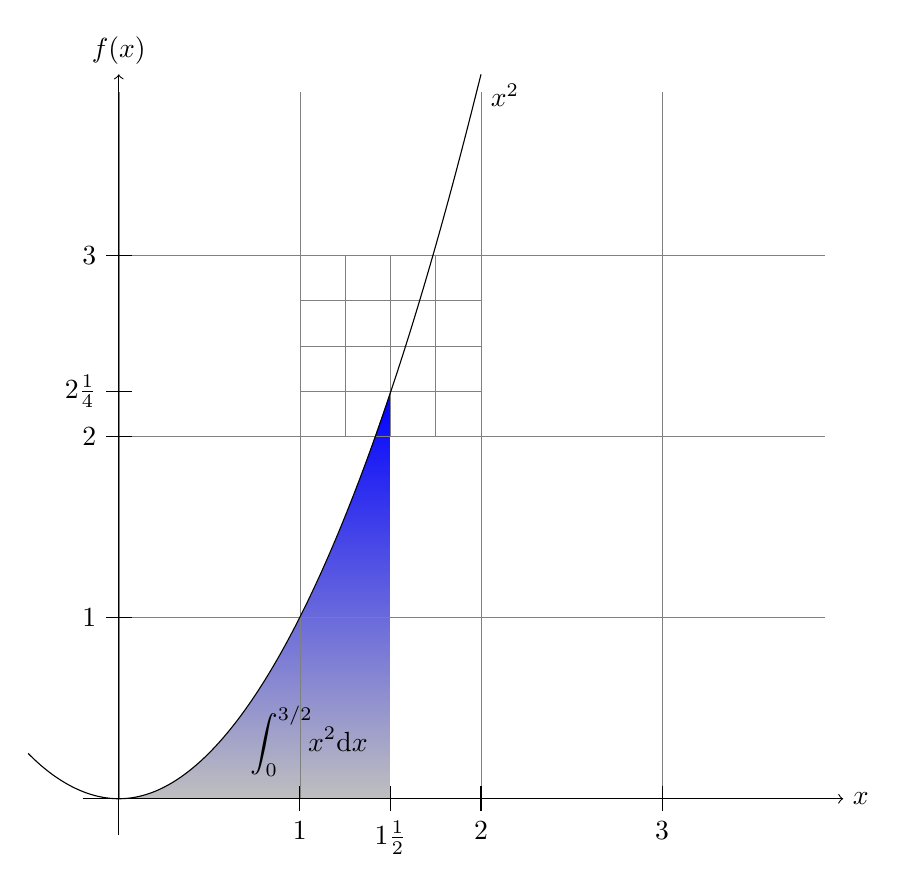
\begin{tikzpicture}[scale=2.3]
		  \shade[top color=blue,bottom color=gray!50] 
		      (0,0) parabola (1.5,2.25) |- (0,0);
		  \draw (1.05cm,2pt) node[above] 
		      {$\displaystyle\int_0^{3/2} \!\!x^2\mathrm{d}x$};
		
		  \draw[style=help lines] (0,0) grid (3.9,3.9)
		       [step=0.25cm]      (1,2) grid +(1,1);
		
		  \draw[->] (-0.2,0) -- (4,0) node[right] {$x$};
		  \draw[->] (0,-0.2) -- (0,4) node[above] {$f(x)$};
		
		  \foreach \x/\xtext in {1/1, 1.5/1\frac{1}{2}, 2/2, 3/3}
		    \draw[shift={(\x,0)}] (0pt,2pt) -- (0pt,-2pt) node[below] {$\xtext$};
		
		  \foreach \y/\ytext in {1/1, 2/2, 2.25/2\frac{1}{4}, 3/3}
		    \draw[shift={(0,\y)}] (2pt,0pt) -- (-2pt,0pt) node[left] {$\ytext$};
		
		  \draw (-.5,.25) parabola bend (0,0) (2,4) node[below right] {$x^2$};
		\end{tikzpicture}
		\end{center}
		
		Intuitively, it is obvious that when $a=b$ we extend the definition as follows:
		
		Finally, notice that it is quite possible that the result of the integral to be negative or even complex since it is an algebraic surface! That is to say the result can be in general in $\mathbb{C}$.
	\begin{tcolorbox}[title=Remarks,colframe=black,arc=10pt]
	\textbf{R1.} Other letters rather than $x$ can be used in the evaluation of the definite integral. So if $f$ is integrable on $[a, b]$, then $\int\limits_a^bf(x)\mathrm{d}x=\int\limits_a^bf(t)\mathrm{d}t=\int\limits_a^bf(s)\mathrm{d}s$, etc. This is why the variable $x$ is sometimes named "\NewTerm{dummy variable}\index{dummy variable}".\\

	\textbf{R2.} As we will see below, it is essential not to confuse between a "\NewTerm{definite integral}\index{definite integral}" and a "\NewTerm{indefinite integral}\index{indefinite integral}". Thus, an indefinite integral, denoted $\int\limits f(x)\mathrm{d}x$ is a function, or more precisely, a family of functions also named "\NewTerm{primitives of $f$}\index{primitive of a f unction}" (see below) while a definite integral, denoted $\int\limits_a^b f(x)\mathrm{d}x$ is considered as a constant.
	\end{tcolorbox}
	Let us present a second approach for the definition of the integral, somewhat more rigorous than the previous one  (following the request of several readers). We will use this time, by tradition the $S$ surface instead of the area $A$.
	
	Let f be a bounded function on $[a, b]$. We consider a subdivision $\sigma$ of its support $[a, b]$ that we note:
	
	where the intervals are not necessarily of equal sizes.

	We write for $i=1,2,3,...,n$:	
	
	
	\textbf{Definitions (\#\mydef):}
	\begin{enumerate}
		\item[D1.] We name "\NewTerm{lower Darboux sum}\index{lower Darboux sum}" associated with $f$ and $\sigma$ the surface:
		
		\begin{figure}[H]
			\centering
			\includegraphics{img/algebra/darboux_inferior_sum_concept.jpg}
			\caption{Principle of calculating the lower Darboux sum}
		\end{figure}
		\item[D1.] We name "\NewTerm{upper Darboux sum}\index{upper Darboux sum}" associated with $f$ and $\sigma$ the surface:
		
		\begin{figure}[H]
			\centering
			\includegraphics{img/algebra/darboux_superior_sum_concept.jpg}
			\caption{Principle of calculating the upper Darboux sum}
		\end{figure}
	\end{enumerate}
	A function $f$ is said to be "\NewTerm{Riemann-integrable on $[a, b]$}" if and only if the above two surfaces coincide when the intervals become infinitely small.
	
	All Riemann-integrable functions on $[a, b]$ are denoted by $\mathcal{R}_{[a,b]}$.
	
	Darboux sums are not very useful for the effective calculation of an integral, for example using a computer, because it is usually quite difficult to find the $\inf$ and $\sup$ on sub-intervals. Rather, we consider:
	
	The "\NewTerm{Riemann sum}\index{Riemann sum}" is defined from the fact that we if denote a "\NewTerm{partition}\index{partition}" (or "\NewTerm{regular partition}" if they all have the same width) of the interval $[a,b]$ by:
	
	and that:
	
	where $\xi_i \in [x_{i-1},x_i]$, then:
	
	But as we must choose an $\xi_i$, we often takes either the right or the left one, thus taking randomly the "method of left rectangles":
	
	Which would give us the example below:
	\begin{figure}[H]
		\centering
		\includegraphics{img/algebra/left_rectangle_integral.jpg}
		\caption{Principle of calculating methods using left rectangles}
	\end{figure}
	either:
	
	But it is easy for a step function... but it is less so for a continuous function for which we will obtain only an approximate value of the actual surface! The idea is then to take intervals smaller and smaller:
	\begin{figure}[H]
		\centering
		\includegraphics{img/algebra/riemann_integral_left_rectangle.jpg}
		\caption{Principle of the calculation of the Riemann integral with left rectangles method}
	\end{figure}
	And then, at the limit, we obtain the desired quantity:
	
	The fact to search this limit is named "calculate the integral," and more specifically for the chosen method: "calculate the Riemann integral".
	
	\begin{tcolorbox}[colframe=black,colback=white,sharp corners]
	\textbf{{\Large \ding{45}}Example:}\\\\
	We want to use the construction of the definite integral to evaluation:
	
	using a right-endpoint approximation to generate the Riemann sum.\\
	
	For this purpose we first set up the Riemann sum. Based on the limits of integration, we have $a=0$ and $b=2$. For $i=0,1,2,\ldots,n$, let $P=\{x_i\}$ be a regular partition of $[0,2]$. Then:
	
	Thus, the function value at the right endpoint of the interval is:
	
	Then the Riemann sum takes the form:
	
	Using the Gauss summation relation of $\displaystyle\sum_{i=1}^n i^2$ (\SeeChapter{see section Sequences and Series page \pageref{sum of squares integers}}), we have:
	
	Now, to calculate the definite integral, we need to take the limit as $n\rightarrow+\infty$. We get:
	 
	\end{tcolorbox}
	
	\subsubsection{Indefinite Integral}
	We have seen before in our study of derivatives the following problem: given a function denoted by $F(x)$, find its derivative $f(x)$, that is to say the algebraic function:
	
	\textbf{Definition (\#\mydef):} We say that the function $F (x)$ is a "\NewTerm{primitive}\index{primitive}" or "\NewTerm{indefinite integral}\index{indefinite integral}" of the function $f (x)$ on any segment $[a, b]$ if at any point in any segment we have $F'(x)=f(x)$.
	
	Tow more explicit and less technical alternative definitions are: 
	\begin{itemize}
		\item An "indefinite integral" is a FUNCTION of $x$ (or another variable), while a "definite integral" is a VALUE!
		
		\item The collection of all antiderivatives of $f(x)$ is named the "indefinite integral" of $f$ with respect to $x$.
	\end{itemize}

	
	Another way to see the indefinite integral concept is to go through the "\NewTerm{fundamental theorem of integral and differential calculus}\index{fundamental theorem of integral and differential calculus}" also sometimes named "\NewTerm{fundamental theorem of calculus}\index{fundamental theorem of calculus}\label{fundamental theorem of calculus}" whose two properties are stated as follows:
	\begin{enumerate}
		\item If $A$ (area) is the function defined by $A(X)=\displaystyle\int\limits_a^X f(t)\mathrm{d}t$ for each $X$ in any $[a, b]$, then $A$ is the primitive of $f$ on $[a, b]$ which is zero in $a$ (or in other words: $f (t)$ is the derivative of $A$).
		\item If $F$ is a primitive of $f$ on any $[a, b]$, then:
		
		that can also be written obviously as following:
		
	\end{enumerate}
	Let us prove the first property of this fundamental theorem:
	\begin{dem}
	Given the function:
	
	If $f$ is positive, and $h>0$ (the proof in the case where $h<0$ is similar) and as $X>0$, we know that we can think of $A(X)$ as the area under the curve of $f$ from $t=a$ to $t=X$.
	\begin{figure}[H]
		\centering
		\includegraphics{img/algebra/area_primitive_representation.jpg}
		\caption{Graphical representation of the area}
	\end{figure}
	To show that $A$ is a primitive of $f$, we will prove that $A'=f$. According to the definition of the derivative:
	
	Let us study this quotient: $A(x+h)-A(x)$ is represented by the area of the strip of width $h$, sandwiched between two rectangles of width $h$.
	
		Given $M$ the maximum of $f$ on the interval $[X,X+h]$ and $m$ the minimum interval of $f$ over the same interval. The respective areas of the two rectangles are $Mh$ and $mh$.
	
	We then have the following double inequality:
	

	As $h$ is positive, we can divide by $h$ without changing the meaning of  the inequalities:
	
	When $h\rightarrow 0^+$ and if $f$ is a continuous function, then $M$ and $m$ have for limit $f (X)$, and the ratio:
	
	which is between $m$ and $M$, has effectively for limit $f(X)$.
	
	As $A'(X)=f(X)$ for all $X$, this shows that the derivative of the area function is $f$. And therefore $A$ is an indefinite primitive of $f$. As $A(a)=0$, $A$ is effectively the primitive of $f$ which vanishes on $a$.
	\begin{flushright}
		$\square$  Q.E.D.
	\end{flushright}
	\end{dem}
	Before starting the proof of the second properties of the fundamental theorem, let us give and prove the following theorem that will we be essential to us: If $F_1(x)$ and $F_2(x)$ are two primitives of $f(x)$ on any segment $[a, b]$, their difference is a constant (this result is very important in physics in terms of the study of what we name the "initial conditions").
	\begin{dem}
	We have after the definition of the concept of Primitive:
	
	for $\forall x \in [a,b]$.
	
	Let us write:
	
	We can write:
	
	So it comes from what we saw during our study of derivatives that:
	
	Then we have:
	
	\begin{flushright}
		$\square$  Q.E.D.
	\end{flushright}
	\end{dem}
	It follows from this theorem that if we know any primitive $F (x)$ of the function $f (x)$ any other primitive of this function will be of the form:
	
	where $c^{te}$ is named the "\NewTerm{constant of integration}\index{constant of integration}\label{constant of integration}".
	
	So finally, we name "\NewTerm{indefinite integral}\index{indefinite integral}" of $f (x)$ and we denote by:
	
	any expression of the form $F (x)+c^{te}$ where $F(x)$ is a primitive of $f(x)$. Thus, by writing convention:
	
	if and only if $F'(x)=f(x)$.
	
	In this context, $f (x)$ is also named "\NewTerm{integrand function}\index{integrand function}" and $f (x) \mathrm{d}x$, the "\NewTerm{function under the sum sign}".
	\begin{tcolorbox}[title=Remark,colframe=black,arc=10pt]
	An "\NewTerm{antiderivative}\index{antiderivative}" of a function $f$ is one function $F$ whose derivative is $f$. The indefinite integral of $f$ is the set of ALL antiderivatives of $f$. Therefore indefinite integral and antiderivative is not the same as the first is the set of all the seconds! If $f$ and $F$ are as described just now, the indefinite integral of $f$ has the form $\{F+c^{te}|c^{te}\in\mathbb{R}\}$ when an antiderivative is just one element of this set!! But not all teachers are according on the definition of antiderivatives...
	\end{tcolorbox}
	
	Geometrically, we can consider the indefinite integral as a set (family) of curves as we move from one to another by performing a translation in the positive or negative direction of the axis.
	
	Let us return to the proof of item (2) of the fundamental theorem of integral (and differential) calculus:
	\begin{dem}
	Let $F$ be a primitive of $f$. Since two primitives differ by a constant, we have well:
	
	that we can also write:
	
	for all $X$ in $[a, b]$. The particular case $X=a$ gives $\int\limits_a^a f(t)\mathrm{d}t$ and therefore $F(a)+c^{te}=0$ and we get obviously $c^{te}=-F(a)$. Substituting, we get:
	
	As this identity is valid for all $X$ in the interval $[a,b]$ it is true especially for $X=b$. Therefore:
	
	\begin{flushright}
		$\square$  Q.E.D.
	\end{flushright}
	\end{dem}
	This last result also shows something useful!: It is not necessary when we evaluate and integral to take into account the constant of the general primitive since it is canceled by the difference of the two primitives!!
	\begin{tcolorbox}[title=Remarks,colframe=black,arc=10pt]
	\textbf{R1.} The above fundamental theorem that shows the link between primitive and integral led us to use the same symbol $\int$ to write a primitive (introduced by Leibniz in the late 17th century), which is a function, and an integral that it is a number.\\
	
	\textbf{R2.} We also proved in the section of Analytical Mechanics using an integral how to calculate the full length of a curve in the plane if the function $f(x)$ is explicitly known.
	\end{tcolorbox}
	Here are some trivial properties of integration that is good to remember because often used elsewhere in this book (if it do not seem obvious to you, contact us and we will give the detailed proof):
	\begin{enumerate}
		\item[P1.] The derivative of an indefinite integral is equal to the integrand:
		
		\item[P2.] The differential of an indefinite integral is equal to the expression under the integral sign:
		
		\item[P3.] The indefinite integral of the differential of a given function is equal to the sum of this function and an arbitrary constant:
		
		\item[P4.] The indefinite integral of the sum (or subtraction) of two or more algebraic functions is equal to the algebraic sum of their integral (do not forget that we work with the set of all primitives and not a specific given one primitive!):
		
		\begin{dem}
		To prove this, following the request of a reader, we will prove that the derivative of the left-hand side allows us to find the derivative of the right-hand side and vice versa (reciprocal) with the above properties.
		
		According to P1 we have:
				
		Let us check if it is the same with the right-hand side (we assume known the properties of derivatives that we proved earlier in this section):
		
		\end{dem} 
		\begin{flushright}
			$\square$  Q.E.D.
		\end{flushright}
		\item [P5.] We can get out a constant factor from the integral sign, that is to say:
		
		We justify this equality by deriving the two members (and according to the properties of derivatives):
		
		\item[P6.] We can take out a constant factor in the argument of the integrated function (rather rarely used):
		
		Indeed, by differentiating both members of equality we have following the properties of derivatives:
		
		\item[P7.] The integration of a function whose argument is summed (or subtracted) is algebraically the primitive of the argument summed (respectively subtracted):
		
		This property can be showed identically to the previous one using also the derivatives properties.
		\item[P8.] The combination of properties P6 and P7 allows us to write:
		
		\item[P9.] Let $f$ be a continuous function on $[a, b]$, we have for all $c$ belonging to this interval:
		
		This theorem, sometimes named "\NewTerm{Chasles relation}\index{Chasles relation}" (by its vector equivalent) follows directly from the definition of the indefinite integral. $F$ being a primitive of $f$ on $[a, b]$ we have:
		
		\item[P10.] This is a property often used in the section of Statistics (we do not find an easy way to express this property by everyday language so...):
		
		 Let us see now two properties that will be helpful we sometimes to calculate difficult integrals:
		\item[P11.] If a function is even (\SeeChapter{see section Functional Analysis page \pageref{even function}}), the integral on symmetrical bounds is equivalent to:
		
		\item[P12.] If a function is odd (\SeeChapter{see section Functional Analysis page \pageref{odd function}}), the integral on symmetrical bounds is equivalent to:
		
		
		\item[P13.] The integral of a periodic function is invariant under a shift of its integration. This is a property that we will use further below to finalize the proof of the integral representation of the zero order Bessel function of the first type:
	
		If $f$ is a periodic function of period $T$ we know that any value $a$:
		
		So now consider:
		
		We do the change of variable $y=t-T$, the we have for the last integral:
		
		Therefore:
		
	\end{enumerate}
	
	\pagebreak
	\subsubsection{Double Integral}
	The idea of double integrals is to measure the volume of the area bounded by the graph of a function of two variables over a domain $D$ of the plane (below $D$ is rectangular):
	\begin{figure}[H]
		\centering
		\includegraphics{img/algebra/double_integral_square_domain.jpg}
		\caption{Example of a continuous function of two variables over a squared domain}
	\end{figure}
	It could be obvious to the reader that double integrals are extremely important in the field of Applied Mathematics!
	
	Again, the idea is the same as the definite integral. If we adapt a simplistic approach, we decompose the continuous function like a staircase and the volume to calculate is then reduced to the sum of the volumes of parallelepipeds:
		
	\begin{figure}[H]
		\centering
		\includegraphics{img/algebra/double_integral_square_domain_decomposition_into_big_parallelepipeds.jpg}
		\caption{Volume decomposition into big parallelepipeds}
	\end{figure}
	Therefore we have the double sum:
	
	For a continuous function, we proceed by successive approximations: we calculate the Riemann sums for subdivisions always thinner and thinner of the domain $D$:
	\begin{figure}[H]
		\centering
		\includegraphics{img/algebra/double_integral_square_domain_decomposition_into_thin_parallelepipeds.jpg}
		\caption{Decomposition of the volume in always thinner parallelepipeds}
	\end{figure}
	and therefore at the limit:
	
	But..., when want want to integrate an area that is not rectangular, things get a priori more complicated ... Let's see a workaround.
	
	For this purpose, we will build closed bounded domain $D$ as follows:
	
	where the reader will have noticed that the support is the variable $x$ by trough the two functions $u$ and $v$. This then is what we name a "\NewTerm{type I domain}\index{domain of definition!type I domain}" (and therefore if it is $y$ that parameterizes $x$ then it is "\NewTerm{type II domain}\index{domain of definition!type II domain}").

	This can be illustrated by the figure below:
	\begin{figure}[H]
		\centering
		\includegraphics{img/algebra/double_integral_type_I_domain_example.jpg}
		\caption{Example of a type I domain}
	\end{figure}
	where we notice that this simplistic approach (there are other possible approaches but that need the use of Measurement Theory) requires that the domain is simply convex\footnote{As we have seen in the section of Geometric Shapes an area is convex if any couple of points on the bounds of the area with a crossing line has this latter no outside of the area} (that is to say they are no holes outside the domain $D$ between $u (x)$ and $v (x)$) or decomposed into simply convex disjoint subdomains.

	
	To resume, we can integrate as follows:
	
	So we transform the double integral in two nested simple integrals.
	
	\paragraph{Fubini's theorem}\label{fubini theorem}\mbox{}\\\\
	We will see now an important theorem used repeatedly in different section of this book and which permits to reverse the order of integration.
	
	Remembering that:
	
	we can also use:
	
	So with this parametrization we can write:
	
	We can change the order of integration, the calculation is different, but the result is the same. But that's not what really interests us here!
	
	Consider a function such as (we say that the function can be "variable separable"):
	
	Therefore:
	
	Suppose that the domain is a rectangle (we do this simplification otherwise the proof complicates considerably). Meaning:
	
	Therefore the integral linearity property:
	
	
	\subsubsection{Integration by Substitution}
	When we can not easily determine the primitive of a given function, we can find sometimes, with a smart change of variables (sometimes very subtle...), bypass the difficulty. It does not work every time (because some functions are not formally integrable) but it is worth a try before taking out your computer.
	
	Again, we give only the general form of the method. It is the role of teachers in schools to train, and train, and train students to understand and master these techniques. In addition, the sections in this book that treats of exact sciences (physics, computer science, astrophysics, chemistry, ...) replete with examples using this technique and thus serve implicitly as exercises.
	
	Consider we want to calculate the integral (not bounded for the moment):
	
	although we do not know directly how to calculate the primitive of this function $f(x)$ (at least we imagine being in that situation) we know (in one way or another) that exists (we do treat of improper integrals at this level).

	The technique then consists in this integral to perform the following change of variable:
	
	where $\varphi (t)$ is a continuous function and also its derivative, and having an inverse function. Then $\mathrm{d}x=\varphi' (t)\mathrm{d}t$, and let us prove now that in this case the equality:	
	
	is satisfied.
	\begin{dem}
	We imply here that the variable $t$ will be replaced after integration of the right member by its expression in function of $x$. To justify this equality in this sense, it suffices to show that the considered amounts where each is a defined only with a difference of a given arbitrary constant have the same derivative with respect to $x$. The derivative of the left member is:
	
	We derive only the right member with respect to $x$ considering that $t$ is a function of $x$. We know that:
	
	We get therefore:
	
	\begin{flushright}
		$\square$  Q.E.D.
	\end{flushright}
	\end{dem}
	Obviously, the function $x=\varphi (t)$ must be chosen so that we know how to calculate the indefinite integral on the right side of equality.
	\begin{tcolorbox}[title=Remark,colframe=black,arc=10pt]
	Sometimes it is preferable to choose the change of variable in the form $t=\varphi (x)$ instead of $x= \psi(t)$ because as this to a large tendency to simplify the length of the equation instead of making it longer.
	\end{tcolorbox}
	It is obvious that this theorem will be more explicitly written:
	
	
	\pagebreak
	\paragraph{Jacobian}\label{jacobian}\mbox{}\\\\
	Consider a domain $D$ of the plane  $u,v$ delimited by a curve $L$. Suppose that the $x, y$ coordinates are functions of the new variables $u, v$ (always in the context of a change of variables!) by the following relations:
	
	where the functions $\varphi (x,y)$ and $\phi(u,v)$ are unique, continuous and have continuous derivatives in a given domain $D'$ which we will define later. It corresponds therefore following previous relations to any pair of values $u, v$ only one couple of values $x, y$ and vice versa.
	
	It follows from what was said just before that at any point $P(x,y)$ of the plane $\text{O}xy$  corresponds univocally a point $P '(u, v)$ of the plane $\text{O}uv$ of coordinates $u, v$ defined by the above relations. The numbers $v$ and $u$ will be named "\NewTerm{curvilinear coordinates}\index{curvilinear coordinates}\label{curvilinear coordinates}" of $P$ and we will see concrete and schematics examples of these in the section of Vector Calculus.
	
	If in the $X\text{O}Y$ plane the set of points $P$ describes a closed curve $L$ defining a domain $D$, the corresponding set of points describes in $u\text{O}v$ a given domain $D'$. It corresponds to any point of $D'$ a point of $D$. Thus, the relations of transformation establish a bi-univocal correspondence between the points of the domains $D$ and $D'$.
	
	Now consider in $D'$ a straight line of equation $u=c^{te}$. In general, the relations of transformation make it corresponds in the plane $\text{O}xy$ a curved line (or vice versa). Therefore, let us cut the domain $D'$ by the multiple straight lines of equations $u=c^{te}$ and $v=c^{te}$ into small rectangular areas (we will not take into account at the limit, the rectangles on the boundary of $D'$). The corresponding curves of the domain $D$ then cut this latter it into quadrilateral (defined by curves therefore). Obviously, the reverse applies!
	
	Consider in the plane $\text{O}uv$ the rectangle $\Delta s'$ limited by the straight lines:
	
	and the curvilinear quadrilateral corresponding $\Delta s$ in the plane $\text{O}xy$. We will designate areas of these partial domains also  by $\Delta s'$ by $\Delta s$. We have obviously:
	
	The areas $\Delta s$ and $\Delta s'$ are different in general.
	 \begin{figure}[H]
		\centering
		\includegraphics[scale=0.8]{img/algebra/non_linear_map.jpg}
		\caption{A nonlinear map $f : \mathbb{R}^2\mapsto \mathbb{R}^2$ sends a small square to a distorted parallelogram}
	\end{figure}
	Suppose in $D$ a continuous function $z=f(x,y)$. It corresponds to any value of this function of the domain $D$ the same value $z=F(u,v)$ (what we want to check) in $D'$, where:
	
	Consider the integrals sum of the function $z$ in the domain $D$. We obviously have the following equality:
	
	Let us calculate $\Delta s$, that is to say the area of the curvilinear quadrilateral $P_1,P_2,P_3,P_4$ in the plane $\text{O}xy$:
	
	We determine the coordinates of its vertices:
	
	
	We will assimilate in the calculation of the are of the quadrilateral  $P_1,P_2,P_3,P_4$ the arcs $P_1P_2,P_2P_3,P_3P_4,P_4P_1$ to parallel line segments. We will also replace the increasing values of the functions by their differentials. This means that we ignore the infinitely small differentials of higher order than $\Delta u$ and $\Delta v$. The previous relations then become:
	

	Under these assumptions, the curvilinear quadrilateral $P_1P_2P_3P_4$ can be likened to a parallelogram. His area is therefore approximately equal to twice the area of the triangle $P_1P_2P_3$, area that we can calculate by using the properties of the determinant (as we will prove it in the section on Linear Algebra, in $\mathbb{R}$ the determinant  represents a parallelogram while in $\mathbb{R}^2$ it represents the volume of a parallelepiped):
	
	Such as (this is here that the best choice has to be done so that the final expression is the simplest and most aesthetic, for this purpose we proceed by trials and finally we make the choice below):
	\begin{figure}[H]
		\centering
		\includegraphics{img/algebra/graphical_representaton_of_determinant.jpg}
		\caption{Graphical representation of the determinant}
	\end{figure}

	Thus we have:
	
	Therefore the following relation (containing what is usually named the "\NewTerm{functional determinant}\index{functional determinant}"):
	
	with:
	
	that is the "\NewTerm{Jacobian matrix}\index{Jacobian matrix}" (its determinant is simply named the "\NewTerm{Jacobian}\index{Jacobian}" (for short)) of the coordinate transformation $\mathbb{R}^2 \rightarrow \mathbb{R}^3$. By applying exactly the same reasoning to $\mathbb{R}^3$, then the Jacobian is written (by changing some notations because otherwise it becomes unreadable):
	
	In short, what it is useful exactly? Well let us come back to our relation:
	
	which is finally only an approximation because in the calculations of the area $\Delta s$ we neglected the infinitely small differential of higher order. However, more the dimensions of the elementary domains $\Delta s$ and $\Delta s'$ are small, and more we are approaching the true equality. The equality finally taking place when we go to the limit (finally also in math we make approximations... eh!), the surfaces of the elementary domains tending to zero:
	
	We apply now the equality obtained to calculate the double integral (we can do the same with the triple of course). So we can finally write (this is the only way of putting the thing that makes sense):
	
	Passing to the limit, we obtain the strict equality:
	
	This is the coordinate transformation relation in a double integral! It allows us to reduce the calculation of a double integral in the domain $D$ to domain $D'$, which can simplify the problem.
	Similarly, for a triple integral, we write:
	
	
	\begin{tcolorbox}[colframe=black,colback=white,sharp corners]
	\textbf{{\Large \ding{45}}Examples:}\\\\
	Let us now determine the Jacobian for the most common coordinate systems (we send the reader back again to Vector Calculus section for more information about these systems):\\
	
	E1. Polar coordinates\label{jacobian in polar coordinates} $x=r\cos(\phi),y=r\sin(\phi)$:
	
	Since $r$ is always positive, we simply write:
	
	\end{tcolorbox}
	\pagebreak
	
	\begin{tcolorbox}[colframe=black,colback=white,sharp corners]
	E2. In cylindrical coordinates $x=r\cos(\phi),y=r\sin(\phi),z=z$ (see section Linear Algebra  page \pageref{determinant} for the calculation of such a determinant):
	
	Since $r$ is always positive, we simply write:
	\\
	
	E3. \label{jacobian spherical coordinates}In spherical coordinates $x=r\sin(\theta)\cos(\phi),y=r\sin(\theta)\sin(\phi),z=r\cos(\theta)$ (see section Linear Algebra  page \pageref{determinant} for the calculation of such a determinant):
	
	Since $r$ is always positive, we simply write:
	
	\end{tcolorbox}

	\subsubsection{Integration by Parts}\label{integration by parts}
	When we seek to make integrations, it is very common that we have to use a tool (or calculation method) named "\NewTerm{integration by parts}\index{integration by parts}". There are different degrees of use of this tool and we'll start with the most simple and that is the most used in all chapters and sections in this book.
	
	First we start from the derivative of the product of two functions proved above:
	
	
	so we have:
	
	and we get:
	
	after a final simplification we finally get the famous very important equality:
	
	But sometimes we will need the generalization of that relation. We can show that if $f$ and $g$ are two applications (functions) of class $\mathcal{C}^n$ ($n$ times differentiable) on $[a, b]$ in $\mathbb{C}$, then:
	
	\begin{dem}
	Let us proceed by induction on n$ $(beware it is not necessarily easy to understand as often with demonstrations by induction!).
	
	Knowing the relation is true for $n = 1$, we assume it true for $n$ (as given in the above relation!) and we prove it for $n + 1$ (so we must laid on the previous relation but with $n + 1$ instead of $n$):
	
	\begin{tcolorbox}[title=Remark,colframe=black,arc=10pt]
	The trick (proposed by a reader) in this proof is to see that $-(-1)^n$ gives a minus sign when $n$ is even and plus sign when $n$ is odd and also that $+(-1)^{n+1}$ gives a minus sing when $n$ is even and plus sign when $n$ is odd.
	\end{tcolorbox}
	For $n = 1$ we fall back on the well known and very often used equality in this book:
	
	\begin{flushright}
		$\square$  Q.E.D.
	\end{flushright}
	\end{dem}

	\pagebreak
	\subsubsection{Usual Primitives}\label{usual primitives}
	There are in math and physics many primitives or functions defined on integrals we see  quite frequently (but not exclusively). Furthermore, all primitive proved below will be used in the various chapters on Mechanics, Engineering, Atomistic, Social Mathematics, etc of this book. So, as in any formula booklet, we propose you the most sixty knows primitives but with... the proofs!
	
	However, we will omit the primitives that can be immediately deduced from the usual derivatives we have proved above. This means for example that we assume  known two very important primitives (certainly the most used in all pages of this book):
		
	Otherwise here is the list of the most common primitives (the reader will meet anyway many others - developed in the details - as it reads this book):
	\begin{enumerate}
		\item Primitive of $f(x)=\tan (x)$:
		
		By definition we have:
		
		We use the change of variable $u=\cos(x),\mathrm{d}u=-\sin(x)\mathrm{d}x$ and therefore:
		
		Therefore:
		
		\item Primitive of $f(x)=\cot(x)$:
		
		By definition we have:
		
		We use the change of variable $u=\sin(x),\mathrm{d}u=\cos(x)\mathrm{d}x$ and therefore:
		 
		Therefore:
		
		\item Primitive of $f(x)=\arcsin(x)$:
		
		We integrate by parts:
		
		If we put $u=1-x^2$, giving us $\mathrm{d}u=-2x\mathrm{d}x$, we get:
		
		Therefore:
		
		\item Primitive of $f(x)=\arccos(x)$:
		
		We integrate by parts again:
		
		If we put $u=1-x^2$, giving us $\mathrm{d}u=-2x\mathrm{d}x$, we get:
		
		Therefore:
		
		\item Primitive of $f(x)=\arctan(x)$:
		
		We integrate by parts again:
		
		If we put $u=1+x^2$, giving us $\mathrm{d}u=2x\mathrm{d}x$, we get:
		
		Therefore:
		
		\item Primitive of $f(x)=\text{arccot}(x)$:
		
		Once again... we integrate by part:
		
		If we put $u=1+x^2$, giving us $\mathrm{d}u=2x\mathrm{d}x$, we get:
		
		Therefore:
		
		\item Primitive of $f(x)=xe^{ax}$ with $a\in \mathbb{R}\left\lbrace 0 \right\rbrace$:
		
		An integration by part gives:
		
		Therefore:
		
		The generalization is in our point of view immediate and we get the following reduction formula:
		
		\begin{tcolorbox}[title=Remark,colframe=black,arc=10pt]
		Another very important primitive with the exponential in physics is that we had proved in our study of the law of Gauss-Laplace law (Normal Law) in the section of Statistics (determination of the expected mean).
		\end{tcolorbox}
		\item Primitive of $f(x)=\ln(x)$:
		
		We write:
		
		Integrating by parts we found:
		
		Finally:
		
		\item Primitive of $f(x)=x\ln(ax)$ with $a\in \mathbb{R}\left\lbrace 0 \right\rbrace$:
		
		An integration by part give us:
		
		Therefore:
		
		\item Primitive of $f(x)=a^x$ for $a>0,a\neq 1$:
		
		To begin we write:
		
		Therefore we get:
		
		and:
		
		Finally:
		
		\item Primitive of $f(x)=\log_a(x)$:
		
		For $a>0,a\neq 1$ knowing that (see the properties of logarithms in the section of Functional Analysis):
		
		we get using the primitive of $\ln(x)$:
		
		\item Primitive of $f(x)=\tanh(x)$:
		
		We have:
		
		we use the change of variables $u=\cosh(x),\mathrm{d}u=\sinh(x)\mathrm{d}x$ and we get:
		
		Finally:
		
		\item Primitive of $f(x)=\coth(x)$:
		
		We know we have:
		
		we use the change of variables $u=\sinh(x),\mathrm{d}u=\cosh(x)\mathrm{d}x$ and we get:
		
		Finally:
		
		\item Primitive of $f(x)=\text{arcsinh}(x)$:
		
		We integrate by parts:
		
		If we put $u=1+x^2,\mathrm{d}u=2x\mathrm{d}x$ we get:
		
		Finally:
		
		\item Primitive of $f(x)=\text{arccosh}(x)$:
		
		If we integrate by parts as before:
		
		If we put $u=1-x^2,\mathrm{d}u=-2x\mathrm{d}x$ we get:
		
		Finally:
		
		\item Primitive of $f(x)=\text{arctanh}(x)$:
		
		We integrate by parts:
		
		If we put $u=1-x^2,\mathrm{d}u=-2x\mathrm{d}x$ we get:
		
		Finally:
		
		\item Primitive of $f(x)=\text{arccoth}(x)$:
		
		We integrate by parts:
		
		If we put $u=1-x^2,\mathrm{d}u=-2x\mathrm{d}x$ we get:
		
		Finally:
		
		\item Primitive of $f(x)=\sin ^{n}(x)$ with $n \geq 2$:
		
		Let us put $I_n=\int \sin ^n(x)\mathrm{d}x$. An integration by parts give:
		
		substituting $\cos ^2(x)$ by $1-\sin ^2{x}$ in the last primitive, we obtain:
		
		and therefore:
		
		All primitives of the same form (recurrence relation) are named "\NewTerm{reduction formulas}\index{reduction formulas}".
		
		\item Primitive of $f(x)=\cos ^{n}(x)$ with $n \geq 2$:
		
		In this case we have the recursive formula:
		
		that is proved exactly in the same way as the previous recursive relation (the reader can request the details if required).
		\item Primitive of $f(x)=\tan ^{2}(x)$:
		
		Knowing that $\tan'(x)=1+\tan^2(x)$ we have:
		
		Therefore:
		
		\item Primitive of $f(x)=\cot ^{2}(x)$:
		
		Knowing that $\cot'(x)=-1-\cot^2(x)$ we have:
		
		Therefore:
		
		\item Primitive of $f(x)=\sin ^{-2}(x)$:
		
		Using remarkable trigonometric identities (\SeeChapter{see section Trigonometry page \pageref{remarkable trigonometric identities}}), we have:
		
		Thanks to the primitive of $\cot^2(x)$. Therefore:
		
		\item Primitive of $f(x)=\cos ^{-2}(x)$:
		Using once again remarkable trigonometric identities (\SeeChapter{see section Trigonometry page \pageref{remarkable trigonometric identities}}), we have:
		
		Thanks to the primitive of $\tan^2(x)$. Therefore:
		
		\item Primitive of $f(x)=\sin ^{-1}(x)$:
		
		We use the substitution $x=2\arctan(t),t=\tan(x/2)$. Knowing that (\SeeChapter{see section Trigonometry page \pageref{remarkable trigonometric identities}}):
		
		we then get:
		
		Therefore:
		
		Finally:
		
		\item Primitive of $f(x)=\cos ^{-1}(x)$:
		
		Knowing that $\cos(x)=\sin(x+\pi/2)$ (\SeeChapter{see section Trigonometry page \pageref{remarkable angles}}) we have:
		
		We do the change of variable $x+\pi/2=u, \mathrm{d}u=\mathrm{d}x$:
		
		thanks to the knowledge of the primitive of $\sin ^{-1}(x)$. Finally:
		
		\item Primitive of $f(x)=\dfrac{1}{1+\cos(x)}$:
		
		We do the substitution $x=2\arctan(t),t=\tan(x/2)$, knowing that (\SeeChapter{see section Trigonometry page \pageref{remarkable trigonometric identities}}):
		
		we get:
		
		Therefore:
		
		Finally:
		
		\item  Primitive of $f(x)=\dfrac{1}{1-\cos(x)}$:
		
		We do again the substitution $x=2\arctan(t),t=\tan(x/2)$. Then we find:
		
		So that finally:
		
		\item  Primitive of $f(x)=\dfrac{1}{1+\sin(x)}$:
		
		Knowing that:
		
		we can write:
		
		By making the change of variables:
		
		we get:
		
		Finally:
		
		\item  Primitive of $f(x)=\dfrac{1}{1-\sin(x)}$:
		
		By the same reasoning as above using the cosine we get:
		
		
		\item Primitive of $f(x)=\sinh^n(x)$ with $n \geq 2$:
		
		Let us put:
		
		An integration by parts gives (we proved during our study of usual derivatives that the primitive of the hyperbolic sine was the hyperbolic cosine):
		
		by substituting $\cosh^2(x)$  and $1+\sinh^2(X)$ in the last integral, we obtain:
		
		and therefore:
		
		Therefore we obtain easily the special case:
		 
		\item Primitive of $f(x)=\cosh^n(x)$ with $n \geq 2$:
		
		In this case we also have the recurrence relation:
		
		that is proved in the same way as above. So we also get easily the special case:
		
		
		\item Primitive of $f(x)=\tanh^2(x)$:
		
		Knowing that (proved during our study of usual derivatives):
		
		we have:
		
		Therefore:
		
		
		\item Primitive of $f(x)=\coth^2(x)$:
		
		Knowing that (proved during our study of usual derivatives):
		
		we have:
		
		Therefore:
		
		
		\item Primitive of $f(x)=\dfrac{1}{\sinh^2(x)}$:
		
		We have using the primitive of $f(x)=\coth^2(x)$:
		
		Therefore:
		
		
		\item Primitive of $f(x)=\dfrac{1}{\cosh^2(x)}$:
		
		We have using the primitive of $f(x)=\tanh^2(x)$:
		
		Therefore:
		
		
		\item Primitive of $f(x)=\dfrac{1}{\sinh(x)}$:
		
		We do the substitution:
		
		We get using the derivative of $\text{arctanh}(x)$:
		
		
		and finally:
		
		
		\item Primitive of $f(x)=\dfrac{1}{\cosh^2(x)}$:
		
		We do the substitution:
		
		We get using the derivative of $\arctan(x)$:
		
		and finally:
		
		\item Primitive of $f(x)=\dfrac{1}{1+\cosh(x)}$:
		
		We do the substitution:
		
		We get:
		
		Finally we get:
		
		
		\item Primitive of $f(x)=\dfrac{1}{1-\cosh(x)}$:
		
		We do the substitution:
		
		We get:
		
		Finally:
		
		
		\item Primitive of $f(x)=\dfrac{1}{1+\sinh(x)}$:
		
		We do the substitution:
		
		We get:
		
		But:
		
		Therefore:
		
		Therefore:
		
		
		\item Primitive of $f(x)=\dfrac{1}{1-\sinh(x)}$:
		
		We still do the same substitution:
		
		We get:
		
		But:
		
		Therefore:
		
		Finally:
		
		
		\item Primitive of $f(x)=e^{ax}\sin(bx)$ with $a,b\in \mathbb{R},a^2+b^2\neq 0$:
		
		A first integration by parts gives:
		
		A second integration by parts gives
		
		So we have the equality:
		
		Therefore redistributing the previous relation:
		
		
		\item Primitive of $f(x)=e^{ax}\cos(bx)$ with $a,b\in \mathbb{R},a^2+b^2\neq 0$:
		
		A similar reasoning than before shows that (we can detail on demand as always!):
		
		
		\item Primitive of $f(x)=x\sin(ax)$ with $a \in \mathbb{R}^*$:
		
		And integration by parts gives us:
		
		
		\item Primitive of $f(x)=x\cos(ax)$ with $a \in \mathbb{R}^*$:
		
		And integration by parts gives us:
		
		
		\item Primitive of $f(x)=\dfrac{1}{(x-a)(x-b)}$ with $a \neq b$:
		
		We have the following relation (in integral calculus we name such decomposition a "\NewTerm{partial fraction decomposition}\index{partial fraction decomposition}"):
		
		Therefore:
		
		
		Finally:
		
		
		\item Primitive of $f(x)=\dfrac{1}{a^2-x^2}$ with $a \neq 0$:
		
		We have using the previous result:	
		
		Therefore:
		

		\item Primitive of $f(x)=\dfrac{1}{a^2+x^2}$ with $a \neq 0$:
		
		Doing a change of variable:
		
		We get using the derivative of $\arctan (x)$:
		
		
		\item Given:
		
		with $n \in \mathbb{N}$. We get:
		
		But this last primitive can be solved by parts:
		
		Therefore:
		
		What we find most frequently in the literature under the form:
		
		Identically to the next development, we have for (the sign change):
		
		the following relation:
		
		You can find an application of these two primitives in the Newtonian cosmological model of the Universe in the section of Astrophysics and also in the section of General Relativity in the study of the Shapiro effect!
		
		\item Primitive of $f(x)=\dfrac{1}{(1-x^2)^2}$:
		
		We have using the primitives of $\dfrac{1}{(1-x^2)^n}$ (proved before) and of $\dfrac{1}{1-x^2}$ (also proved above):
		
		
		\item Primitive of $f(x)=\dfrac{1}{(1+x^2)^2}$:
		
		We have using the primitives of $\dfrac{1}{(1+x^2)^n}$ (proved before) and of $\dfrac{1}{1+x^2}$ (also proved above):
		
		
		\item Primitive of $f(x)=\sqrt{x^2-a^2}$ with $a\in \mathbb{R}^*$ (case relative to the area under a hyperbola):
		
		We can assume without loss of generality $a>0$. Note that the domain of definition of $f$ is $]\infty,-a] \cup [a,+\infty[$.
		
		We will determine now a primitive of $f$ only on the interval $[a,+\infty[$ (because that is it we will need in some sections of this book).
		
		Let us make the change of variable:
		
		So with:
		
		where we consider the function $\cosh: \mathbb{R}^+ \rightarrow [1,+\infty[$ with for reciprocal the function $\text{arccosh}:[1,+\infty[ \rightarrow \mathbb{R}^+$ given by (\SeeChapter{see section Trigonometry page \pageref{inverse hyperbolic to logarithm}}):
		
		We obtain then using then primitive of $\sinh^2(x)$:
		
		but \SeeChapter{see section Trigonometry page \pageref{hyperbolic trigonometry}}) as:
		
		Therefore:
		
		and using another identity proved in the section Trigonometry:
		
		we have therefore:
		
		as the primitive are given to a given constant, we can write:
		
		for $x\geq a$. $F$ is then a primitive of $\sqrt{x^2-a^2}$ on the interval $[a,+\infty[$.
		
		\item Primitive of $f(x)=\sqrt{a^2-x^2}$ with $a\in \mathbb{R}^*$:
		
		We can assume without loss of generality $a>0$. Note that the domain of definition of $f$ is $[-a, a]$.
		
		We make the substitution:
		
		we get:
		
		where we used the primitive $\cos^n (x)$ with $n=2$ proved above. Now we have:
		
		Then:
		
		and:
		

		\item Primitive of $f(x)=\sqrt{x^2+a^2}$ with $a\in \mathbb{R}^*$:
		
		We can assume without loss of generality $a>0$.
		
		Let us make the change of variable:
		
		with:
		
		We get:
		
		Therefore:
		
		But as we saw in the section on Trigonometry page \pageref{hyperbolic trigonometry}:
		
		and:
		
		Finally we have:
		
		where $ln (a)$ has been omitted because the primitives are given to a given constant.
		
		\item Primitive of $f(x)=\left(\sqrt{a^2-x^2}\right)^{-1}$ with $a\in \mathbb{R}^*$:
		
		We can assume without loss of generality $a>0$.
		
		We do the substitution:
		
		We get:
		
		
		\item Primitive of $f(x)=\dfrac{1}{\sqrt{a^2+x^2}}$ with $a\in \mathbb{R}^*$:
		
		We can assume without loss of generality $a>0$.
		
		We do the substitution:
		
		We get in the same manner as the previous usual integrals:
		
		and knowing that (\SeeChapter{see section Trigonometry page \pageref{inverse hyperbolic to logarithm}}):
		
		We then get finally the following important primitive:
		
		Proceeding in the same way, but using the hyperbolic cosine instead of hyperbolic sine, we get obviously (we can detail on demand as always):
		
		We will reuse these last two relation in important practical cases of the section of Analytical Mechanics, Civil Engineering (where the constant $a$ is equal $1$, $\ln(a)$ will be equal to $0$) and General Relativity (where $a$ will be nonzero and therefore it will not be possible to omit the constant $\ln(a)$).
		
		\item In mathematics, there are several integrals known as the "\NewTerm{Dirichlet integral}\index{Dirichlet integral}\label{Dirichlet integral}". One of those is the improper integral of the sinc function over the positive real line:
	
	By Fubini's Theorem (see \pageref{fubini theorem}):
	
	Then using the primitive of $e^{ax}$:
	
	and using the primitive of $e^{ax}\sin(bx)$:
	
	Hence:

	Using the primitive of $\frac{1}{x^2+a^2}$ seen earlier:
	
	As:
	
	Then:
	
		
		\item Let us consider an integral of the following form that we can use to improve the Stirling formula (\SeeChapter{see section Theoretical Computing page \pageref{stirling}}) and also that we need absolutely for the study of the circular Fresnel aperture diffraction (\SeeChapter{see section Wave Optics page \pageref{wave optics}}):
		
		where
		\begin{itemize}
			\item $\lambda$ is large;
			\item $g(y)$ is a smooth function which has a local minimum at $y^*$ in the interior of the interval $[a, b]$;
			\item $h(y)$ is smooth.
		\end{itemize}
		The integral can be the moment generating function of the
		distribution of $g(Y)$ when $Y$ has density $h$ (\SeeChapter{see section Statistics}), it could be a posterior expectation of $h(Y)$, or just a "simple" integral.
		
		When $\lambda$ is large, the contribution to this integral is essentially entirely by construction originating from a neighborhood around $y^*$.
		
		We formalize this by Taylor expansion of the function $g$ around $y^*$ :
		
		Since $y^*$ is a local minimum, we have:
		
		 and therefore:
		
		Therefore:
		
		The fact that above the bounds have change from $[a,b]$ to $]-\infty,+\infty[$ is that we assume that the area of interest is around $y^*$ and that because $\lambda$ is soooo large that veeeery quickly a bit away from $y^*$ we can consider the curve as negligible!
		
		If we approximate $h(y)$ linearly around $y^*$, that is to say:
		
		such that:
		
		Therefore:
		
		The reader must not forget that here $\lambda g''(y^*)$ is a constant and that if we put:
		
		Then for the first integral above we see that we fall back on the integral of something very similar to the Gauss distribution (with mean $y^*$ and standard deviation $\lambda g''(y^*)$) and then it comes almost immediately (\SeeChapter{see section Statistics page \pageref{Gauss integral}}):
		
		For the second integral:
		
		the change of variable $y-y^*=x$ give us:
		
		I is immediate that primitive is of the form:
		
		Therefore by symmetry the second integral is zero! We have finally:
		
		This calculation is named "\NewTerm{Laplace's Method of Integration}\index{Laplace's Method of Integration}\label{laplace method of integration}" or simply "\NewTerm{Laplace Integration}".
	\end{enumerate}
	
	\subsubsection{Integral representation of first kind Bessel's function}\label{integral representation of first kind Bessel's function}
	A particularly useful and powerful way of treating Bessel functions employs their integral representation as we will see in the section of Wave Optics.
	
	Remember that in the section of Sequences and Series we have proved that the generating function of Bessel's function was:
	
	That is:
	
	Now remember that (\SeeChapter{see section Numbers page \pageref{euler formula}}):
	
	So if we return to the generating function, and substitute $t=e^{\mathrm{i}\theta}$, we get:
	
	In which to condensate the result we have used first the property proved during our study of the generating function of Bessel's functions:
	
	and also:
	
	and so on...
	Now remember that:
	
	Therefore identifying real and imaginary part, we get:
	
	Remember also that we have proved during our study of Fourier series in the section of Sequences and Series that:
	
	\begin{center}
	\begin{tabular}{ccc}
	$\text{with }n,k\in \mathbb{N}\text{ and }n\ne k$
	&$\qquad$&
	$\text{with }n,k\in \mathbb{N}\text{ and }n = k$
	\end{tabular}
	\end{center}
	That is:
	
	where $\delta_{nm}$ is the Kronecker symbol (\SeeChapter{see section Tensor Calculus page \pageref{kronecker symbol}}).
	
	Now let us write:
	
	Let us focus on the first integral:
	
	So we see above that whatever the value for any $n$, excepte of $n=0$:
	
	Therefore in only remains for $n>0$:
	
	and we see above that if $n>0$ is odd all the integrals vanish but if $n>0$ is even, only the corresponding $J_n(x)$ remains!
	
	Exactly the same analysis can be done for can be done:
	
	We have therefore for each of the integrals above, especially for each the left term that (recall that $n=0,2,4,\ldots$ is even and $n=1,3,5,\ldots$ is odd):
	
	If these two equations are added together we have using trigonometric identities (\SeeChapter{see section Trigonometry page \pageref{remarkable trigonometric identities}}):
	
	for $n=0,1,2,3,\ldots$.
	
	If we put $n=0$ in the above relation, we get:
	
	If we plot $\cos(x\sin(\theta))$ we see that it repeats itself in all four quadrants (it's an even function):\\\\
	\texttt{>plot([cos(sin(theta)),cos(2*sin(theta)),cos(3*sin(theta)),cos(5*sin(theta))]\\
	,theta=-2*Pi..2*Pi);}
	\begin{figure}[H]
		\centering
		\includegraphics[scale=0.55]{img/algebra/cos_sin_maple.jpg}
	\end{figure}
	So we can write:
	
	This is the real integral representation of the zero order Bessel function of the first type.
	
	But in many developments we don't use the above expression as there is not phasor that is visible. So the trick is to notice that $\sin(x\sin(\theta))$ reverses its sign in the third an fourth quadrant (it's and odd function):\\\\
		\texttt{>plot([sin(sin(theta)),sin(2*sin(theta)),sin(3*sin(theta)),sin(5*sin(theta))],\\
	theta=-2*Pi..2*Pi);}
	\begin{figure}[H]
		\centering
		\includegraphics[scale=0.6]{img/algebra/sin_sin_maple.jpg}
	\end{figure}
	So we have:
	
	Adding the both relations by multiplying the second by $\mathrm{i}$,  we have:
	
	Finally we get the complex representation of the zero order Bessel function of the first type:
	
	
	Let us do a change of variable $\theta=\varphi+\pi/2$, then:
	
	But we have proved earlier that for any periodic function:
	
	Therefore:
	
	This integral representation my be obtained in various ways but this one seems the most easy one to us. Many other integral representation exists.

	\subsubsection{Dirac Function}
	The Dirac function, also named "\NewTerm{Dirac peak}\index{Dirac peak}\label{dirac function}" or "\NewTerm{delta function}\index{delta function}", plays a very important practical role both in electronic and computer also  wave mechanics and quantum field theory (this allows to discretize a continuum!).
	
	Before going further we could notice that it is wrong to speak about a "function" because a function is an application of a start set (usually the set of real or complex number with one or more dimensions) in an arrival set (usually the set of real or complex numbers in one or more dimensions). While the domain of definition of the Dirac function is not a set of numbers but strictly speaking a set of functions!
	
	More technically the Dirac delta function, or $\delta$ function, is a generalized function, or distribution, on the real number line that is zero everywhere except at zero, with an integral of one over the entire real line. The delta function is sometimes thought of as an infinitely high, infinitely thin spike at the origin, with total area one under the spike, and physically represents the density of an idealized point mass or point charge. It was introduced by theoretical physicist Paul Dirac. In the context of signal processing it is often referred to as the unit impulse symbol (or function). Its discrete analog is the Kronecker delta function, which is usually defined on a discrete domain and takes values 0 and 1.
	
	As always in this book we will focus here only on the properties we will need to study Applied Mathematics stuffs of other sections of the book.
	
	To represent mentally in an easy way this function, first consider the function defined by:
	
	The representation of $y=f(x)$ above is a rectangle of width $a$, and of height $1/ a$ and unit surface. The Dirac function can be considered as the boundary when $a\leftarrow 0$ of the  $f (x)$. So we have:		
	
	That is to say:
	\begin{figure}[H]
		\centering
		\includegraphics[scale=0.5]{img/algebra/common_dirac_peak_representation.jpg}
		\caption[Schematic representation of the Dirac delta function by a line surmounted by an arrow]{Schematic representation of the Dirac delta function by a line surmounted by an arrow (source: Wikipedia)}
	\end{figure}
	with:
	
	where $\varepsilon$ is a number greater than $0$ and as small as we want.
	\begin{tcolorbox}[title=Remark,colframe=black,arc=10pt]
		As the reader will have probably noticed it when we introduced the initial function $f (x)$, the resulting delta Dirac function has therefore the dimension of the inverse of a length!
	\end{tcolorbox}
	For a function $g (x)$ continues in $x = 0$ we have:
	
	By extension we have:
	
	and for a function $g (x)$ coninue on $x_0$:
	
	It is then relatively easy to define the Dirac function in 3-dimensional space by:
	
	As as already mentioned we will prove properties of the Dirac function only if we will need them in other sections of this book.
	
	\subsubsection{Gamma Euler Function}\label{gamma euler function}
	We define the Euler Gamma function (Eulerian integral of the second kind) by the following integral:
	
	with $x$ belonging to the set of complex numbers whose real part is positive and non-zero (thus the positive real number are also included in the domain of definition)! Indeed, if we take complex numbers with a zero or negative real part, the integral diverges and is then undefined!
	
	\begin{tcolorbox}[title=Remark,colframe=black,arc=10pt]
		We have already met this integral and some of its properties (which will be proved here) in our study of the Beta, Gamma, Chi-square, Fisher and Student statistical distribution functions (\SeeChapter{see section Statistics page \pageref{statistical distributions}}). We will also use this integral in maintenance (\SeeChapter{see section Industrial Engineering page \pageref{preventive maintenance}}), in String theory and other engineering and physics fields (see the corresponding chapters) as for the canonical negative binomial generalized linear regression (\SeeChapter{see section Theoretical Computing page \pageref{regression techniques}}).
	\end{tcolorbox}
	
	Here is a graphical plot of the module of the Euler Gamma function for $x$ browsing an interval of real numbers (take care in Maple 4.00b to write GAMMA capitalized!!!):
	
	\texttt{>with(plots):\\}
	\texttt{>plot(GAMMA(x),x=-Pi..Pi,y=-5..5);}
	\begin{figure}[H]
		\centering
		\includegraphics{img/algebra/maple_gamma_euler_2d_plot.jpg}
		\caption{Plot of the Euler Gamma function in Maple 4.00b}
	\end{figure}
	and always the same function with Maple 4.00b but now in the complex plane and always with in ordinate the module of the Gamma Euler function:
	
	\texttt{>with(plots):\\}
	\texttt{>plot3d(abs(GAMMA(x+y*I)),x=-Pi..Pi,y=-Pi..Pi,view=0..5, grid=[30,30],orientation=[-120,45],axes=frame,style=patchcontour);}
	
	\begin{figure}[H]
		\centering
		\includegraphics{img/algebra/maple_gamma_euler_3d_plot.jpg}
		\caption{Plot of the Euler Gamma function in the complex plane with Maple 4.0}
	\end{figure}
	This function is interesting if we impose the variable $x$ to belong to the set of integer numbers and that we write it as follows:
	
	Let us integrate by part the latter function:
	
	Since the exponential function decreases much faster than $t^x$ then we have:
	
	In literature, we frequently find the following notations (there are confusing):
	
	Which brings us to write the result in a more traditional form:
	
	From the relation $\Gamma_{0}(x)=x\Gamma_{0}(x-1)$, it comes by induction:
	
	But:
	
	That gives:
	
	Therefore:
	
	or written in another way for $x\in \mathbb{N}^*$
	
	Another interesting and useful result of the Euler gamma function is obtained when we replace $t$ by $y^2$ and calculate this latter for $x=0.5$.
	
	First we have:
	
	and after:
	
	But, as we have proved it in the section Statistics during our study of  the distribution, this integral is equal to:
	
	
	\pagebreak
	\paragraph{Euler-Mascheroni Constant}\mbox{}\\\\
	This small text is a just curiosity regarding to Euler's constant $e$ and to almost every Differential and Integral calculus tools that we have seen until now. This is a very nice example (almost artistic) of what we can do with mathematics as soon as we have enough tools at our disposal.
	
	Moreover, this constant is useful in some differential equations which we see later.
	
	Remember that we saw in the section of Functional Analysis that the Euler constant $e$ is defined by the limit:
	
	
	In a more general case we can easily demonstrate in the same way that (you can ask us the details if needed):	
	
	This obviously suggests:
	
	by a change of variable $t=nu$ we write:
	
	And we use the definition of the Beta function:
	
	Therefore:
	
	To transform this expression we can write:
	
	But the quantity:
	
	tends to the limit $\gamma=0.5772$, named "\NewTerm{Euler-Mascheroni constant}\index{Euler-Mascheroni constant}" or also "\NewTerm{Euler Gamma constant}\index{Euler Gamma constant}" when $n$ tends to infinity.
	
	Therefore:
	
	We divide each term of the product $(x+1)...(x+n)$ by the corresponding integer taken into $n!$, so we get (according to a reader request we have put a maximum of details!):
    
	
	\pagebreak
	\subsubsection{Curvilinear Integrals}\label{curvilinear integral}
	The line integrals (curvilinear integrals) are also very important in physics. The reader will thus find see them again in the section of Classical Mechanics, Electrodynamics Magnetostatics and to calculate the work of a force or the "flow field", or in the chapter of Euclidean Geometry to calculate the center of gravity of curves (functions), or in the section of Geometric Shapes to calculate the surface of some bodies of revolution but also in Corpuscular Quantum Physics for the famous "path integral" (which is only the term used by physicists to say "line integral") or for the specific calculation of integrals using the residue theorem proved in the section of Complex Analysis or for transformation states in the section of Thermodynamics. This is why there will not be here examples of line integrals because they are already so many applications in the other chapters of this book.
	
	With the definition of these integrals, we can prove two very important results detailed in section of Vector Calculus that are respectively the Green's theorem and Stokes' theorem or even the theorem of residues proved in the section Complex Analysis and already mentioned in the preceding paragraph (this is important enough to mention it twice!).
	
	More technically a line integral is an integral where the function to be integrated is evaluated along a curve. The terms "\NewTerm{path integral}\index{path integral}", "\NewTerm{curve integral}\index{curve integral}", and "\NewTerm{curvilinear integral}\index{curvilinear integral}" are also used; "\NewTerm{contour integral}\index{contour integral}" as well, although that is typically reserved for line integrals in the complex plane.
	
	\paragraph{Curvilinear Integral of a scalar field}\mbox{}\\\\
	Consider a parametrized curve $C$ (\SeeChapter{see section Differential Geometry page \pageref{parametric curves}}) by a vector function $\vec{r}(t)$ with $t \in [a,b]$ of class $\mathcal{C}^1$ piecewise (this condition is necessary so that we can integrate the curve without problems).
	
	\textbf{Definitions (\#\mydef):}
	 \begin{enumerate}
	 	\item[D1.] The curve is said to be a "\NewTerm{closed curve}\index{closed curve}" if $\vec{r}(a)=\vec{r}(b)$
	 	
	 	\item[D2.] The curve is said to be a "\NewTerm{smooth curve}\index{smooth curve}" if $\forall t \in [a,b]\; \vec{r}'(t)\neq 0$
	 \end{enumerate}
	 Recall that a parametric curve can be written as follows (all vector function can be written in this form):
	 
	Consider a function or a "\NewTerm{scalar field}\index{scalar field}" $f(x,y)$ defined in a neighborhood of $C$. We subdivide $[a,b]$ into $n$ subintervals of equal length $\Delta t$ as:
	
	We choose on each subinterval a point $t_i^*\in [t_i,t_{i+1}]$. Given $\delta s_i$ the length of the arc $C$ connecting the point $(x(t_i),y(t_i))$ and $(x(t_{i+1}),y(t_{i+1})$, the integral of $f$ along $C$ is defined as the "\NewTerm{line integral}\index{line integral}" or "\NewTerm{path integral}\index{path integral}":
	
	Which as we know, can be written (see section of Differential Geometry page \pageref{curvilinear abscissa helix} of Analytical Mechanics page \pageref{parametric curve length} and many others):
	
	and that can obviously be immediately extended to the case to 3 variables and more.
	
	Or in vector form:
	
	The line integral is linear, that is to say, if $C=C_1 \cup C_2$ and that $C_1 \cap C_2$ is a point, then (without going into the strict definition of the union of two curves...):
	
	
	\paragraph{Curvilinear Integral of a vector field}\mbox{}\\\\
	Consider a vector field (e.g. a force field) as:
	
	and an infinitesimal element of a curve (path) $\mathcal{C}^1$ piecewise as:
	
	The idea is then to consider that the dot product (vector field projection on the path element) represents the work along the differential element:
	
	Therefore the work on all the path will be given by (using the property of linearity of the curvilinear integral):
	
	This can obviously be generalized to $n$ dimensions. Let us indicate that when the line integral (path integral) of a vector field is extended to a closed curve, then we speak of "\NewTerm{circulation of the vector field}\index{circulation of the vector field}".
	
	As:
	
	We then have write a fairly common notation:
	
	\begin{tcolorbox}[title=Remark,colframe=black,arc=10pt]
	In physics many times problems are often in the plane and require the transition to polar coordinates because many academic physic problems are centro-symmetric, which also facilitates the calculations of path integrals.
	\end{tcolorbox}
	
	\begin{tcolorbox}[colframe=black,colback=white,sharp corners]
	\textbf{{\Large \ding{45}}Example:}\\\\
	Let us calculate the work of the force of gravity moving a mass $M$ of the point $M_1(a_1,b_1,c_1)$ to the point $M_2(a_2,b_2,c_2)$ along an arbitrary path $C$. The projections of the force of gravity on the coordinate axes are:
	
	The work accomplish is then:
	
	so we find a very known result of the section of Classical Mechanics.
	\end{tcolorbox}
	A line integral of a vector $\vec{F}$ field along a curve $C_1$ is independent of the path of integration if:
	
	for any non-null curve $C_2$ having only the same points of departure and arrival. Furthermore if the vector field satisfied (where $U$ in physics is typically a potential):
	
	as (the reader will recognize an exact total differential form):
	
	Then the integral path on an arbitrary curve only depends only on the difference of the values the function $U$ at the two ends! This is the "\NewTerm{fundamental theorem for line integrals}\index{fundamental theorem for line integrals}" or "\NewTerm{gradient theorem for line integrals}\index{gradient theorem for line integrals}".
	\begin{dem}
	If the differential form of the vector field satisfies an total exact differential, we have:
	
	That is:
	
	\begin{flushright}
		$\square$  Q.E.D.
	\end{flushright}
	\end{dem}
	So the line integral of an exact total differential does not depend on the path of integration but only the ends! We also conclude that if $\vec{F}$ isderived from a scalar potential and $A = B$, the line integral is then zero.
	
	In physics this result is interpreted by saying that the work provided by a force $\vec{F}$ derived from a scalar potential acting on an elementary particle in a finite displacement does not depend on the path followed.
	
	\textbf{Definitions (\#\mydef):}
	\begin{enumerate}
		\item[D1.] When the curve (path) $C$ is closed and the path integral has a result independent result of the direction in which this path is traveled, we use the following notation (the letter below the symbol representing the path can of course vary...):
		
		If this closed integral is always zero, we say that the integrated vector field is a "\NewTerm{conservative vector field}\index{conservative vector field}" and "\NewTerm{derives from a scalar potential}" (and therefore satisfies the Schwarz's theorem to be written as exact total differential) since this stems from the proof given already just above.
		
		\item[D2.] \label{closed path orientation}When the value of the integral of a closed path depends on the orientation (clockwise not equal to counterclockwise) we use the following notation (the letter below the symbol representing the path can of course vary...):
		
		Thus if the direction is direct (that is to say "counterclockwise" or "trigonometric") as the notation on the above, its sign will be positive; if on the contrary the direction is clockwise his sign will be negative (see the proof in the section of Complex Analysis). Therefore we often speak about respectively "negative direction" or "positive direction".
		
		Thus, to summarize, a line integral (path integral) is fully defined by the expression under the symbol of the integral, the form of integration path and the direction of the integration.
	\end{enumerate}
	\begin{tcolorbox}[title=Remark,colframe=black,arc=10pt]
	The reader will find some the proofs of very important properties of curvilinear integrals  in section of Vector Calculus as the Green-Riemann theorem or a particular application to study holomorphic functions in the section of Complex Analysis.
	\end{tcolorbox}
	
	\subsubsection{Integrals involving parametric equations}
	Now that we have seen how to calculate the derivative of a plane curve, the next question is this: How do we find the area under a curve defined parametrically? 
	
	To derive an expression for the area under a parametric curve defined by the functions:
	
	with $a\leq t\leq b$.

	We assume that $x(t)$ is differentiable and start with an equal partition of the interval $a\leq t\leq b$. Suppose:
	
	and consider the following figure: $x(t_0),x(t_1),x(t_n)$
	\begin{figure}[H]
		\centering
		\includegraphics{img/algebra/integral_parametric_curve.jpg}
	\end{figure}
	We use rectangles to approximate the area under the curve. The height of a typical rectangle in this parametrization is $y(x(\overline{t_i}))$ for some value $\overline{t_i}$ in the $i$-th subinterval, and the width can be calculated as $x(t_i)-x(t_{i-1})$. Thus the area of the $i$-th rectangle is given by:
	
	Then a Riemann sum for the area is:
	
	Multiplying and dividing each area by $t_i-t_{i-1}$ gives:
	
	Taking the limit as $n$ approaches infinity gives:
	
	And it is obvious that applying Pythagoras's theorem on an infinitesimal length of the parametric curve we have:
	
	with $x=x(t)$, $y=y(t)$ and $t_1<t<t_2$. This gives the arc length\index{arc length} of the parametric curve between two points on the curve.
	
	It comes also immediately:
	
	The chain rule gives:
	
	Therefore:
	
	We will meet again this relation in the section of Analytical Mechanics.
	
	In astronomy we often have to deal with closed curved and calculated the distance travel on that curve. But working in cartesian coordinates is not always is the best. This is why it is better to change in polar coordinates.

	The idea is to suppose that we are able to express our curve of interest in the following form:
	
	where $\alpha\leq \theta \leq \beta$. In order to adapt the arc length relation for a polar curve, we use the relations:
	
	and we replace the parameter $t$ by $\theta$ Then:
	
	we replace $\mathrm{d}t$ by $\mathrm{d}\theta$, and the lower and upper limits of integration are $\alpha$ and $\beta$ respectively. Then the arc length formula becomes:
	
	So finally in polar coordinates:
	
	
	\subsubsection{Improper Integrals}
	Improper integrals are definite integrals where one or both of the boundaries is at infinity, or where the integrand has a vertical asymptote in the interval of integration. As crazy as it may sound, we can actually calculate some improper integrals using some clever methods that involve limits.
	
	By abuse of notation, improper integrals are often written symbolically just like standard definite integrals, perhaps with infinity among the limits of integration. When the definite integral exists (in the sense of either the Riemann integral or the more advanced Lebesgue integral), this ambiguity is resolved as both the proper and improper integral will coincide in value and this is what will the most occur through all applications of integrals in physics, chemistry and engineering through this book!
	
	For the Riemann integral (or the Darboux integral, which is equivalent to it as we have seen earlier above), improper integration is necessary both for unbounded intervals (since one cannot divide the interval into finitely many subintervals of finite length) and for unbounded functions with finite integral (since, supposing it is unbounded above, then the upper integral will be infinite, but the lower integral will be finite)!
	
	An "\NewTerm{improper integral}\index{improper integral}" of a function $f(x) > 0$ is:
	
	We say the improper integral converge if this limit exists and diverges otherwise.
	
	Geometrically then the improper integral represents the total area under a curve stretching to infinity. If the integral $\int_a^\infty f(x)\mathrm{d}x$ converges the total area under the curve is finite; otherwise it's infinite.
	
	How can an area that extends to infinity be finite?  Obviously the area between $a$ and $N$ (i.e. $\int_a^N f(x)\mathrm{d}x$) is finite.  As $N$ goes to infinity this quantity will either grow without bound or it will converge to some finite value. 
	
	The domains where improper integrals are the most used, without even be noticeable most of time by students or engineering practitioners, are respectively:
	\begin{itemize}
		\item Statistics (see corresponding section) when we normalize or check the condition of covergence to a cumulated probability of $1$ of a density function (most of time in statistics one or the both bounderies are equal to infinity)

		\item Wave Quantum Physics (see corresponding section) where we deal sometimes with free propagating particles from infinity to infinity (this also happens sometimes in General Relativity)

		\item Differential equations, especially when we solve them by using Fourier Transform or Laplace transform (we have many examples using this transforms accross the book) for practical application in physics and high level financial engineering.

		\item In astrophysics or electrostatics when dealing with any punctual potential field source of the type $1/r^2$  for which we want to calculate the work necessary to bring an object from infinity to that source (calculation of the type $\int_{+\infty}^{r} f(r)\mathrm{d}r$).
	\end{itemize}
	\begin{tcolorbox}[colframe=black,colback=white,sharp corners]
	\textbf{{\Large \ding{45}}Examples:}\\\\
	E1. We want compute the very important integral (to introduce Laplace Transforms):
	
	with $a\in\mathbb{R}$.\\
	
	Following the definition above we need to first compute a definite integral and the take a limit. So from the definition:
	
	We first compute the definite integral. We start with the case $a=0$:
	
	therefore for $a=0$ the improper integral $I$ does not exist. When $a\neq 0$ we have:
	
	In the case $a<0$, that is $a=-|a|$, we have that:
	
	therefore for $a<0$ the improper integral $I$ does not exist. In the case $a>0$ we have:
	
	
	E2. We want to compute:
	
	The integrand is not continuous at $x=0$ and so we’ll need to split the integral up at that point:
	
	
	\end{tcolorbox}
	
	\begin{tcolorbox}[colframe=black,colback=white,sharp corners]
	Now we need to look at each of these integrals and see if they are convergent
	
	At this point we're done.  One of the integrals is divergent that means the integral that we were asked to look at is divergent.  We don't even need to bother with the second integral.
	\end{tcolorbox}
	On a side note, notice that the area under the curve of this infinite interval was not infinity as the reader may have suspected it to be (perhaps).  In fact, it was a surprisingly small number.  Of course this won't always be the case, but it is important enough to point out that not all areas on an infinite interval will yield infinite areas.
 
	Let's now get some definitions out of the way.  We will call these integrals convergent if the associated limit exists and is a finite number (i.e. it's not plus or minus infinity) and divergent if the associated limit either doesn't exist or is (plus or minus) infinity.
	
	\pagebreak
	\subsection{Differential Equations}
	\textbf{Definition (\#\mydef):} In mathematics, a "\NewTerm{differential equation D.E.}\index{differential equation}"  is a relationb etween one or more unknown functions and their derivatives up to order $n$. The "\NewTerm{order}\index{order of a differential equation}" of a differential equation corresponding to the maximum degree of differentiation which one of the functions is subjected.
	
	Compared to our goal of trying to see how the math describes the sensible reality, differential equations are a great success but are also the source of many troubles. First there are modeling difficulties (see for example the differential equation system of General Relativity in the corresponding section of the book...) resolution difficulties (there is no general method even with numerical computer methods as you can see in the corresponding section!), then their are proper mathematical difficulties (that's why some D.E. have million dollar price in case or resolution), finally difficulties related to the fact that certain differential equations are unstable by nature and give chaotic solutions (see the section Population Dynamics or Meteorology for flagrant simple examples!).
	
	\begin{tcolorbox}[title=Remark,colframe=black,arc=10pt]
	The differential equations are used to construct mathematical models of physical orbiological phenomena, such as for the study of radioactivity, celestial mechanics, electronic circuits, populatin development or even financial stochastic process. Therefore, differential equations represent a vast field of study, both in pure and Applied Mathematics.
	\end{tcolorbox}
	The differential equation of order $n$ the more general can always be written as:
	
	We consider in this book only the cases where $x$ and $y$ have their values in $\mathbb{R}$. A solution to such a D.E. on the interval $I \in \mathbb{R}$ is a function $y \in \mathcal{C}^n (I,\mathbb{R})$ (a function $y:I \rightarrow \mathbb{R}$ which is $n$ times continuously differentiable) such that for any $x \in I$, we have:
	
	\begin{tcolorbox}[title=Remarks,colframe=black,arc=10pt]
	\textbf{R1.} For reasons that will be developed later, we also say "integrate a D.E." instead of saying "finding a solution to the D.E.". The first expression is particularly found in the American literature.\\
	
	\textbf{R2.} Since all this book is full examples of differential equations with initial conditions (we speak then about a "\NewTerm{Cauchy problem}\index{Cauchy problem}") and methods of resolutions in the section of Classical Mechanics, Atomic Physics, Cosmology, Econometry, Sequences and series, Industrial Engineering, Statistics, etc., we will not give any application examples here and will focus only on the minimum theoretical useful aspect.
	\end{tcolorbox}
	
	\pagebreak
	\subsubsection{First order differential equations}\label{first order differential equations}
	A differential equation of the first order is therefore a D.E. which involves only the first derivative $y'$.
	
	\textbf{Definition (\#\mydef):} A first order differential equation is named "D.E. of order 1 with separate variables" if it can be written as:
	
	Such a differential equation can be easily integrated. Indeed, we write:
	
	Then symbolically:
	
	\begin{tcolorbox}[title=Remark,colframe=black,arc=10pt]
	We write explicitly here the arbitrary integration constant $c^{te} \in \mathbb{R}$ (which is normally implicitly present in the indefinite integrals) to not forget it!
	\end{tcolorbox}
	So the purpose is first to find the primitives $F$ and $G$ of $f$ and $g$, and then to express it in terms of $x$:
	
	The integration constant is fixed when asked for a given $x=x_0$, we get a particular value of $y(x)=y(x_0)=y_0$. We speak then of "\NewTerm{initial value problem}\index{initial value problem}" or of "\NewTerm{initial conditions}\index{initial conditions}\label{initial conditions}" also abbreviated: IC. So, in other words, initial conditions are values of the solution and/or its derivative(s) at specific points.  As we will see eventually, solutions to ... nice enough ... differential equations are unique and hence only one solution will meet the given conditions. The number of initial conditions that are required for a given differential equation will depend upon the order of the differential equation as we will see.
	
	\subsubsection{Linear differential equations}\label{linear differential equations}
	\textbf{Definition (\#\mydef):} A differential equation of order $n$ is named "\NewTerm{linear differential equation L.D.E.}\index{linear differential equation}" if and only if it is of the form:
	
	with:
	
	Let us now see a property that may seem insignificant at first glance but which will become very important later!
	
	We will prove now that $L$ is a linear application:
	
	and for all $\lambda \in \mathbb{R}$
	
	Then we say that the linear D.E. represent a linear model if the multiples of this function (or any linear combination) are also a solution. Thus, in physics, for a linear system, the amplification of the cause involves an amplification of the effect (the systems are often linear in high-school problems but in reality they are rather the exception!).
	
	For example, the ordinary differential equation of order $2$ of the simple pendulum proved in the section of Classical Mechanics is not linear because it contains a sine term that is not separable.

	\textbf{Definition (\#\mydef):} The linear differential equation (which is the most common in physics):
	
	is named "\NewTerm{homogeneous equation H.E.}\index{homogeneous equation}" or " \NewTerm{equation without second member E.W.S.M.}\index{equation without second member}" (and sometimes "\NewTerm{complementary equation}\index{complementary equation}") associated to:
	
	\begin{theorem}
	We will now prove an important property of H.E.: the set $\left\lbrace S_0 \right\rbrace$ of solutions of the H.E. is the kernel of the linear application $L$ (which means for refresh: $L(S_0)=0$) and the set  $\left\lbrace S \right\rbrace$ of solutions to $L(y)=f(x)$ is given by:
	
	that is to say that the solutions of the form:
	
	where $y_p$ is a "particular/specific solution" to $L(y)=f(x)$ and $y_h$ the "\NewTerm{homogeneous solution}\index{homogeneous solution}" give all the D.E. solutions.
	\end{theorem}
	\begin{dem}
	The first statement will be assumed obvious.
	
	As regards to the second part, any function of the form $y_p+y_h$ is solution of $L(y)=f(x)$.
	
	Indeed it is trivial and it follows from the definition of the kernel concept (\SeeChapter{see section Set Theory page \pageref{kerr}}):
	
	\begin{flushright}
		$\square$  Q.E.D.
	\end{flushright}
	\end{dem}
	What is important also to understand with the linear D.E. with second member, it is that if we find solutions to $L(y)$ with a second given member and solutions to the same D.E. with another different second member, then the sum of all these solutions will be a solution of the D.E. with the sum of the second members!!!\label{sum solutions of differential equations}
	
	\subsubsection{Resolution methods of differential equations}
	There are many ways to solve accurately or approximately linear or non-linear differential equations. Let us give the list of the few methods we will analyze further below by the example (but who are already many, many times in the chapters of Mechanics, Cosmology, Social Sciences and Quantum Physics):
	\begin{itemize}
		\item The "\NewTerm{method of characteristic polynomial of D.E.}\index{Differential equations!method of characteristic polynomial}" (see below) used a bit in every section of the chapter of Mechanics/Quantum Physics/Cosmology/Chemistry and Social Sciences of this book.
		
		\item The "\NewTerm{method of integrating factor}\index{Differential equations!method of integrating factor}" (see also below) for general knowledge but used to this date for practical cases in this book.
		
		\item The "\NewTerm{method of variation of the constant}\index{Differential equations!method of variation of the constant}" (see below) and used to this date only in the section of Industrial Engineering in this book.
		
		\item The "\NewTerm{method of disturbances of D.E.}\index{Differential equations!method of disturbances}" (see below) useful for the wave quantum physics and quantum field theory.
	\end{itemize}
	
	Note also other widely used methods (classical high-school technics) but that are treated case by case in the individual sections of this book because solving approaches are too numerous and specific to each problem:
	
	\begin{itemize}
		\item The "\NewTerm{separation of variables method of D.E.}\index{Differential equations!separation of variables}" (the heat equation in the section of Thermodynamics, wave equation in the section Marine \& Weather Engineering, Schrödinger evolution equation in the section of Wave Quantum Physics, vibration of a drum in the section of Wave Mechanics, etc.), whose we will see a very specific and simple case lower but for which it is best to refer to the sections mentioned for concrete examples.
		
		\item The "\NewTerm{matrix method for solving D.E.}\index{Differential equations!matrix method}" and "\NewTerm{trivial solution of D.E.}" (Lotka-Volterra model in the section of Populations Dynamics, electron or nuclear spin resonance in the section of Relativistic Quantum Physics, Lorenz model in the section of Marine \& Weater Engineering, etc.).
		
		\item The "\NewTerm{spectral method}\index{Differential equations!spectral method}" using the spectral theorem proved in the section of Linear Algebra (see the section of Industrial Engineering for the calculation of system reliability by Markov chains for a concrete example).
		
		\item The "\NewTerm{method of the Fourier transform of the D.E.}\index{Differential equations!Fourier transform method}" or "\NewTerm{method of the Laplace transform of the D.E.}\index{Differential equations!Laplace transform method}" (heat equation in the section Thermodynamics, resolution of the Black \& Scholes equation in the section of Economy, beam equation  under point load in the section of Civil Engineering).
		
		\item "\NewTerm{Numerical methods for D.E.}\index{Differential equations!numerical method}" to solve the differential equations using computer when the D.E. have no known analytic solutions or when they have but we need a visual three dimensional view of the solutions (heat equation in the section of Theoretical Computing).
		
		\item The "\NewTerm{Frobenius method}\index{Differential equations!Frobenius method} named after Ferdinand Georg Frobenius and  also "\NewTerm{power series solutions}\index{Differential equations!power series solutions}, that is a way to find an infinite series solution for a second-order ordinary differential equation of a special form. We will use this technique in the section of Sequences and Series for our study of the Bessel series and also introduce Bessel series by solving in the section of Mechanical Engineering the probel of the self-buckling column with the power series solutions.
	\end{itemize}
	\begin{tcolorbox}[title=Remark,colframe=black,arc=10pt]
	The first differential equations were solved around the end of the 17th century and beginning of the 18th century. By the middle of the 18th century people realized that the first methods we listed above had reached a dead end. One reason was the lack of functions to write the solutions of differential equations. The elementary functions we use in calculus, such as polynomials, quotient of polynomials, trigonometric functions, exponentials, and logarithms, were simply not enough. People even started to think of differential equations as sources to find new functions. It was matter of little time before mathematicians started to use power series expansions to find solutions of differential equations. Convergent power series define functions far more general than the elementary functions from calculus.
	\end{tcolorbox}
	
	\paragraph{Method of characteristic polynomial}\label{method of characteristic polynomial}\mbox{}\\\\
	Solving simple differential equations (with constant coefficients and without second member most of the time...) uses a technique using a characteristic polynomial of the differential equation which we will see the details in the developments that follow on  few special cases very frequent in physics.
	
	It is a relatively simple method to implement when we seek solutions to the homogeneous differential equation without second member (E.W.S.M.). In the contrary case, the presence of a second member, we add the solutions of the homogeneous equation to the particular solutions.
	
	\subparagraph{Resolution of the H.E. of the first order L.D.E. with constant coefficients}\label{first order lde with constant coefficients}\mbox{}\\\\

	Consider the following L.D.E. with constant coefficients:
	
	which is a simplified version of the following general L.D.E.  with constant coefficients:
	
	where:
	
	We write its associated homogeneous equation (E.W.S.M.):
	
	Which can be written:
	
	Therefore:
	
	There is behind this homogeneous solution infinite solutions: to each value given to the constant $C$ there is a solution.
	
	We still need to add to this homogeneous solution the particular solution $y_p$ and for that we have a collection of recipes, depending on the type of the function $f (x)$ of the second member of the differential equation. We will see in each case in the various chapters this book as already mentioned.
	
	\subparagraph{Resolution of the H.E. of the first order L.D.E. with non-constant coefficients}\mbox{}\\\\
	The general solution of homogeneous linear differential equations (E.W.S.M.) of order $1$ with non constant coefficients:
	
	can always be reduced to the following form:
	
	where:
	
	Well obviously there is the solution $y=0$... but let us try to do better. So we have:
	
	It comes therefore:
	
	where $G (x)$ is a primitive of $g (x)$. Since then:
	
	It is also common to find these developments in another notation a little bit more explicit.
	
	So we start again of the differential equation without second member with non-constant coefficients:
	
	after rearrangement:
	
	And then:
	
	Therefore:
	
	This result will be very useful to calculate the Fourier transform of a Gaussian function (\SeeChapter{see section Sequences And Series page \pageref{fourier transform gaussian function}}), Fourier transform, which is essential to resolve in a fairly general way the heat equation (\SeeChapter{see section Thermodynamics page \pageref{heat equation}}) resolution that will finally allow us to prove the Black \& Scholes equation (\SeeChapter{see section Economics page \pageref{solving black and scholes}}). 
	
	\subparagraph{Resolution of the H.E. of the second order L.D.E. with constant coefficients}\mbox{}\\\\\label{second order differential equations}
	Consider the L.D.E. with constant coefficients:
	
	which is a simplified version of the following general L.D.E. with constant coefficients:
	
	where:
	
	We write is homogeneous associated equation (E.W.S.M.):
	
	wherein the function of the second member is zero. We can quite quickly consider a solution of the type (inspiring of the form of the solutions of the first order differential equations):
	
	where $\tau$ is a constant. Which give us therefore:
	
	What we can simplify by:
	
	If our starting assumption is correct, we only have to solve in $K$ this "\NewTerm{characteristic equation (CHARE)}\index{characteristic equation}\label{characteristic equation}"  or "\NewTerm{characteristic polynomial}\index{characteristic polynomial}" of the homogeneous equation to find the homogeneous solution:
	
	whose solutions depend on the sign of the discriminant of the characteristic polynomial\label{discriminant differential equation}:
	
	\begin{itemize}
		\item If the discriminant is strictly positive, that is to say $\Delta>0$:
		
		So we know that the characteristic polynomial has two distinct roots and then we have:
		
		where $K_1\tau=c^{te}$ and $K_2\delta=c^{te'}$. Then we say that the solution is "\NewTerm{delayed}\index{Differential equations!delayed solution}" or "\NewTerm{advanced}\index{Differential equations!advanced solution}" by the values of these constants. But the key is to note that if $y_h(x)$ is a solution, then $y_h(x\pm \Delta x)$ is always a solution!
		
		We then speak of "\NewTerm{general solution of the homogeneous equation}\index{general solution of the homogeneous equation}". There is behind this result an infinity of solutions: to each value given to the constants $A, B$ corresponds a solution.
		
		Physicists also write sometimes this in a particular form by putting
		
		with then:
		
		And using the hyperbolic trigonometric functions (\SeeChapter{see section Trigonometry page \pageref{hyperbolic trigonometry}}):
		
		where finally the possibility to write the homogeneous solution in the form (when we omit the advance or delay $\delta=\tau=0$):
		
		In addition, let us show that the solutions of the E.W.S.M. form a vector space of dimension $2$ (corresponding to the order of our differential equation)!
		
		Indeed:
		\begin{itemize}
			\item The zero function: $y=0$ is a solution of the E.W.S.M. (this is unnecessary to prove because obvious...!)
			
			\item The sum or subtraction of solutions remains a solution (this we have already proved it before)
			
			\item The elements of the basis of a vector space (the solutions of the E.W.S.M.) are linearly independent (that's an interesting property that we will need later!)
		\end{itemize}
		Let us put:
		
		Then:
		
		These relations injected into the E.W.S.M. in generalized form:
		
		Then gives:
		
		We do have indeed a vector space structure.
		
		Let us recall that conversely two functions are linearly dependent if:
		
		\item If the discriminant is strictly positive, that is to say $\Delta=0$: 
		
		The characteristic equation has a real double root $K$.
		
		By going a little fast we would say then:
		
		and that it is over... but that it is forget that the vector base must be formed of two independent solutions!
		
		So the second option is probably... of the form:
		
		Then:
		
		If we inject it into the E.W.S.M. in generalized form:
		
		Then:
		
		That is to say in our case:
		
		But, both actual real values of $K$ are precisely solutions of:
		
		The prior-previous relation is reduced to:
		
		and as we are in the case of study where the discriminant is zero, we have:
		
		Therefore and finally the prior-previous relation reduces to:
		
		We deduce from it that:
		
		Therefore finally:
		
		Which gives for the general solution of the E.W.S.M.:
		
		
		\item If the discriminant is strictly positive, that is to say $\Delta<0$:
		The characteristic equation has two complex conjugate roots (\SeeChapter{see section Calculus page \pageref{second order polynomial roots}}):
		
		Therefore:
		
		But if we look instead for real solutions, we can always put $A$ and $B$ as being equal such as:
		
		And if we set the delay and advance respectively as being zero ($\delta=\tau=0$), so we find the relation available in most books without proof:
		
		where $A'$ and $B'$ are any two real constants. There is another important form of this last relation (often used in electronics, for example). Indeed, it is possible for any $A'$ and $B' \in \mathbb{R}$ , to find $C'$ and $\phi$ also in $\mathbb{R}$ such as the following equality holds:
		
		We put:
		
		Then:
		
		It is then possible to find $\phi$ such as:
		
		Therefore our initial expression (proposition) can be written as:
		
		Finally:
		
	\end{itemize}
	So we can make the following summary:
	To resume:
	\begin{table}[H]
		\begin{center}
			\definecolor{gris}{gray}{0.85}
				\begin{tabular}{|c|c|c|}
					\hline
					\multicolumn{1}{c}{\cellcolor{black!30}\textbf{Discriminant}} & 
	  \multicolumn{1}{c}{\cellcolor{black!30}\textbf{Roots}}  & 
	  \multicolumn{1}{c}{\cellcolor{black!30}\textbf{Homogeneous solution}} \\ \hline
					$\Delta>0$ & \centering\arraybackslash\ $K_{1,2}=\dfrac{-a\pm \sqrt{a^2-4b}}{2}$ & $y_h=Ae^{K_1(x+\tau)}+Be^{K_2(x+\delta)}$ \\ \hline
					$\Delta=0$ & \centering\arraybackslash\ $K_{1,2}=\dfrac{-a\pm \sqrt{a^2-4b}}{2}$  & $y_h=(C_1 x+C_2)e^{K(x+\tau)}$ \\ \hline
					$\Delta<0$ & \centering\arraybackslash\ $K_{1,2}=\dfrac{-a\pm \sqrt{a^2-4b}}{2}$  & $y_h=e^{\alpha x}(A' \cos(\beta x)+B'\sin(\beta x))$ \\ \hline
			\end{tabular}
		\end{center}
		\caption{Typical solutions of H.E. of The L.D.E. with constant coefficients}
	\end{table}
	
	\paragraph{Integrating Factor Method (Euler's Method)}\mbox{}\\\\
	The technique of integrating factor is useful when it comes to solve differential equations of the form:
	
	We have not to this day practical application of this technique in the other chapters of this book. You must therefore see this as a presentation for general culture.
	
	The basic idea is to find a function $M(x)$, named "\NewTerm{integration factor}\index{integration factor}", by which can be multiplied by our differential equation to bring the left-hand side of equality to a simple derivative. For example, for a linear differential equation as the one above, we choose often the following integration factor (but this is by far not the only possibility and this choice does not solve everything!):
	
	Therefore we have:
	
	or by distributing:
		
	Which can therefore be seen as:
	
	or even better (and therein lies the whole trick)...:
	
	We can then take the primitive with respect to $x$:
	
	We can then take the primitive with respect to $x$:
	
	and trivially (!) we have the left primitive that is immediate:
	
	Which is sometimes written as:
	
	\begin{tcolorbox}[colframe=black,colback=white,sharp corners]
	\textbf{{\Large \ding{45}}Example:}\\\\
	Consider the following differential equation:
	
	That we we will rewrite as:
	
	We see then that (assuming $x$ is positive):
	
	Then we have:
	
	Hazard making  sometimes things good (the example is purposely very simple), we have this equality that simplified as:
	
	in:
	
	Which may be condense in:
	
	By integrating:
	
	It then comes immediately:
	
	Finally:
	
	\end{tcolorbox}
	
	\pagebreak
	\paragraph{Method of separation of variables}\label{separation vaiables method}\mbox{}\\\\
	The method of separation of variables (also known as the "\NewTerm{Fourier method}\index{Fourier method}") is any of several methods for solving ordinary and partial differential equations, in which algebra allows one to rewrite an equation so that each of two variables occurs on a different side of the equation.
	
	In mathematics, a "\NewTerm{partial differential equation PDE}\index{partial differential equation}" is a differential equation that contains unknown multivariable functions and their partial derivatives (a special case are ordinary differential equations, which deal with functions of a single variable and their derivatives). PDEs are used to formulate problems involving functions of several variables, and are either solved by hand, or used to create a relevant computer model.
	
	PDEs can be used to describe a wide variety of phenomena such as sound, heat, electrostatics, electrodynamics, fluid dynamics, elasticity, or quantum mechanics. These seemingly distinct physical phenomena can be formalized similarly in terms of PDEs. Just as ordinary differential equations often model one-dimensional dynamical systems, partial differential equations often model multidimensional systems. PDEs find their generalization in stochastic partial differential equations.
	
	A partial differential equation (PDE) for the function $U(x_{1},\cdots ,x_{n})$ is an equation of the form:
	
	If $f$ is a linear function of $U$ and its derivatives, then the PDE is named a "\NewTerm{linear partial differential equation}\index{linear partial differential equation}". Common examples of linear PDEs include the heat equation, the wave equation, Laplace's equation, Helmholtz equation, Klein–Gordon equation, and Poisson's equation (see the chapters of Mechanics, Electrodynamics and Quantum Physics for the study of most of them!).
	
	The method of separation of variables is a very common technique used in physics when we have second-order differential equations. Many useful examples and very detailed are already in the various chapters already mentioned above. Here we will just present a special case just for doing things good but with the minimum subsistence level!
	
	Consider the common case of physical partial differential equation of the type:
	
	The solution of this equation therefore requires finding a function $U$ which depends on $x$ and $y$ such that:
	
	In physics, the idea is then to put that we can always find a said a "separable" solution of the form:
	
	Thus, the differential equation can be written as:
	
	Which can be rewritten as:
	
	Or:
	
	After rearrangement it is use in physics to note this last equality in condensed form:
	
	This equality can only take place if each term is a constant since $X$ depends only on $x$ and Y only on $y$. It comes then:
	
	And each differential equation can then be solved independently of the other and once the solutions found we multiplied them determine the expression of $U$.
	\begin{tcolorbox}[title=Remark,colframe=black,arc=10pt]
	Probably the most beautiful example is the section of Quantum Chemistry.
	\end{tcolorbox}
	
	\paragraph{Method of constant variation}\mbox{}\\\\
	The variation of constants, is a general method to solve inhomogeneous linear ordinary differential equations.

	For first-order inhomogeneous linear differential equations it is usually possible to find solutions via integrating factors or undetermined coefficients with considerably less effort, although those methods leverage heuristics that involve guessing and don't work for all inhomogeneous linear differential equations.

	Variation of parameters extends to linear partial differential equations as well, specifically to inhomogeneous problems for linear evolution equations like the heat equation, wave equation, and vibrating plate equation. In this setting, the method is more often known as "\NewTerm{Duhamel's principle}\index{Duhamel's principle}", named after Jean-Marie Duhamel who first applied the method to solve the inhomogeneous heat equation.
	
	The idea of the method of variation of the constant is as follows: if we have a particular solution affected by constants, we know that depending of the initial conditions thereof are well determined. The idea is then to generalize by putting that these constants are functions. In some cases obviously mathematical developments will show that the functions are necessarily constant.
	
	The idea behind this method is to say that the solutions of the (linear) differential equation with the second member will look like the solutions of the homogeneous equation. As the term on the right will disrupt this solution, we vary only constants (which will therefore no longer be constants), but we remain on the "base" of homogeneous solutions, to seek close solutions. After we check that this "physicist reasoning" gives out all the solutions of the differential equation.
	
	Let us see before studying to the general case a simple example by considering the following differential equation:
	
	for which the particular solution of the homogeneous equation (E.W.S.M.) is (if you need the details not hesitate to ask!):
	
	The method of variation of the constant consist then to put that:
	
	and therefore:
	
	But by the differential equation with the second member, we have:
	
	
	and it follows that:
	
	where we eliminated the integration constant because what we want is a particular solution! The particular general solution (pg) is then the sum of the particular solution and the homogeneous one and this with the variation of the constant:
	
	Thus, generalizing the previous example, so we have a differential equation of the form:
	
	General particular solution will be:
	
	Then we have:
	
	hence injected into the original differential equation:
	
	Therefore after factoring similar terms:
	
	So we have the above relation and the particular solution to the homogeneous differential equation (therefore without second member):
	
	Therefore we find:
	
	and it sufficient then to integrate this equation to find $C_0(t)$. Then, the particular general solution (pg) will be the sum of the particular homogeneous solution and that with the variation of the constant.
	
	\pagebreak
	\subsubsection{Classification of partial differential equations}
	Before we begin, the reader wonders what classifying differential equations can be used for, well, here are the two main arguments for the usefulness of a classification in the order of importance:
	\begin{itemize}
		\item Many books have authors who systematically speak of a differential equation by categorizing it, so it is more pleasant to know what they are talking about

		\item Some finite element modeling software (including MATLAB™) requires that the differential equation category be chosen before anything else can be done as a calculation.
	\end{itemize}
	So this being said, formally, we name "\NewTerm{partial differential equation PDE}\index{partial differential equation}" of order less than or equal to $2$ in a domain $\Omega \subset \mathbb{R}^n$ and of unknown:
	
	An equation of the following general type:
	
 	where $s(x)$ is often named a "\NewTerm{source term}\index{source term}" in analogy with the main situation in physics concerned.

	It is now important to generalize the latter equation in vector form. Thus, we introduce the following notations:
	\begin{itemize}
		\item $A=[a_{ij}]$ the $n\times n$ symmetric matrix of the coefficients in front of the terms of order $2$

		\item $B=(f_i(x))$ The vector of size $n$ of the coefficients in front of the terms of order $1$

		\item $[H\Phi(x)]$ the $n\times n$ symmetric Hessian matrix (\SeeChapter{see section Sequences and Series page \pageref{hessian matrix}}) of $\Phi$:
		

		\item $\vec{\nabla}(\Phi(x))$ the vector of size $n$ of $\Phi$:
		

		\item The notation (named "\NewTerm{Frobenius (matrix) dot product}\index{Frobenius (matrix) dot product}"):
		
	\end{itemize}
	With this, the previous relation:
	
	can be rewritten as:
	
	What is often (abusively) written in a very condensed way:
	
	\begin{tcolorbox}[colframe=black,colback=white,sharp corners]
	\textbf{{\Large \ding{45}}Example:}\\\\
	The following PDE:
	
	First, it is easy to determine (because it is a definition) that:
	
	It is also trivial that:
	
	and that:
	
	It is also trivial that:
	
	Finally, the minor difficulties are to find:
	
	\end{tcolorbox}
	For linear PDE of order $2$, the matrix $A$ is non-zero and is symmetric. It is therefore diagonalizable with real eigenvalues (\SeeChapter{see section Linear Algebra page \pageref{eigenvector}}) and their study provides elements of classification of linear PDE systems of order $2$ under the denomination of "Elliptic", "hyperbolic" or "parabolic" PDE (\SeeChapter{see section Analytical Geometry page \pageref{classification of conical by the determinant}}).

	It is often customary to say in physics that the elliptics PDE characterize problems of equilibrium or stationarity, that hyperbolics PDE characterize problems of wave propagations and finally that parabolic PDE characterize diffusion problems (see examples further below).
	
	That latter terminology comes from the fact that when the matrix $A$ is constant, the curves:
	 
	are respectively ellipsoids, hyperboloid and paraboloid (\SeeChapter{see section Analytical Geometry page \pageref{type of conics matrix approach}}).

	Indeed, we have proved in the section of Analytic Geometry that following the determinant of $A$, we had:
	\begin{itemize}
		\item If $\det(A)=ac-b^2>0$, the curve $\Gamma$ is either empty, reduced to a point, or an ellipse.

		\item If $\det(A)=ac-b^2<0$, the curve $\Gamma$ is either the union of two intersecting lines, that is to say an hyperbola.

		\item If $\det(A)=ac-b^2=0$, the curve $\Gamma$ is either empty, a line, or two distinct parallel lines, or a parabola.	
	\end{itemize}
	More explicitly what we have seen above can be reformulated as following. If we have the following PDE:
	
	where $a$, $b$, $c$, $d$, $e$ and $f$ are real constants is said to be:
	\begin{itemize}
		\item An "\NewTerm{elliptical partial differential equation}\index{elliptical partial differential equation}" if $ac-b^2>0$ that is to say if the eigenvalues are all positive or all negative (\SeeChapter{see section Analytical Geometry page \pageref{type of conics determinant}}).

		\item An "\NewTerm{hyperbolic partial differential equation}\index{hyperbolic partial differential equation}" if $ac-b^2<0$ that is to say there only one negative eigenvalue and all the rest are positive, or there is only one positive eigenvalue and all the rest are negative (\SeeChapter{see section Analytical Geometry page \pageref{type of conics determinant}}).

		\item A "\NewTerm{parabolic partial differential equation}\index{parabolic partial differential equation}\label{parabolic partial differential equation}" if $ac-b^2=0$ that is to say if the eigenvalues are all positive or all negative, save one that is zero (\SeeChapter{see section Analytical Geometry page \pageref{type of conics determinant}}).
	\end{itemize}

	\begin{tcolorbox}[colframe=black,colback=white,sharp corners]
	\textbf{{\Large \ding{45}}Example:}\\\\
	The Laplace's equation:
	
	is an elliptic PDE.\\

	The wave equation:
	
	is a hyperbolic PDE.\\

	The heat equation:
	
	is a parabolic PDE.
	\end{tcolorbox}
	
	\pagebreak
	\subsection{Systems of Differential Equations}
	Let us study now special developments that will also be useful for the study of quantum physics or for the resolution of particular systems of differential equations (see corresponding section in this book for the details on these examples) and especially one which is well known in chaos theory!
	
	Let us first indicate to the reader before going further that more complex inhomogeneous case (with second member) and with unknown coefficients is treated directly by an example in the section of Industrial Engineering during the study of the reliability of a repairable system as a Markov chain with resolution using the determinants and eigenvalues/eigenvectors.
	
	To start this first approach, we will have to introduce the concept of exponentiation of a matrix:

	The set of matrices $n \times n$ with coefficients in $\mathbb{C}$ denoted $M_n(\mathbb{C})$ is a vector space for the addition of matrices and multiplication by a scalar. We will as always denote by $\mathds{1}_n$ the identity matrix of dimension $n$.
	
	We will admit that a sequence of matrices $A_n$ converges to a matrix $A$ if and only if the sequences of coefficients of the matrices $A_n$ converge towards the corresponding coefficients of $A$.
	
	\begin{tcolorbox}[colframe=black,colback=white,sharp corners]
	\textbf{{\Large \ding{45}}Example:}\\\\
	In $M_2(\mathbb{C})$ the sequence of matrice:
	
	converge to:
	
	when $n\rightarrow +\infty$.
	If $x\in \mathbb{C}$, we saw in our study of complex numbers (\SeeChapter{see section on Numbers page \pageref{taylor expansion complex exponential}}) that the series:	
	
	does converge and its limit is denoted by $e^x$. In fact here there is no difficulty in replacing $x$ by a matrix $A$ since we know (we have proved it during our study of complex numbers) that any complex number can be written as follows (the body of complex numbers is isomorphic to the field of real matrices of square dimensions $2$ having this form):
	
	\end{tcolorbox}
	\pagebreak
	\begin{tcolorbox}[colframe=black,colback=white,sharp corners]
	and that a complex number is equivalent to put his matrix form also to the square:
	
	Indeed:
	
	\end{tcolorbox}
	We then define the "\NewTerm{exponential of a matrix}\index{exponential of a matrix}\label{exponential of a matrix}" $A\in M_n(\mathbb{C})$ as the matrix limit of the sequence:
	
	If the matrix $A$ is diagonal obviously its exponential is easy to calculate. Indeed, if:
	
	It follows:
	
	This property of diagonal matrices will also be very useful to us in the section of General Relativity during our study of the variation of the metric determinant.
	
	However, it is clear that a non-diagonal matrix will be much more complicated to deal with! We will then use a diagonalization technique or an endomorphisms reduction\index{endomorphism reduction}\footnote{In linear algebra, an "endomorphism reduction" aims to express matrices and endomorphisms in a simpler form, for example to facilitate calculations. This consists essentially in finding a decomposition of the vector space into a direct sum of stable subspaces on which the induced endomorphism is simpler. Less geometrically, this corresponds to finding a basis of the space in which the endomorphism is simply expressed lile for example the spectral theorem (\SeeChapter{see section Linear Algebra page \pageref{spectral theorem}}).} (\SeeChapter{see section Linear Algebra page \pageref{matrix endomorphism}}) to simplify our problem.
	
	So notice that if $S\in M_n(\mathbb{C})$ is reversible and if $A\in M_n(\mathbb{C})$ then:
	
	This follows from the fact that (think to the change of basis of a linear application as it has been studied in the section of Linear Algebra page \pageref{change of basis}... perhaps it may help):
	
	Therefore:
	
	This development will enable us to bring the computing of the exponential of a diagonalizable matrix in search of its eigenvalues and its eigenvectors.
	\begin{tcolorbox}[colframe=black,colback=white,sharp corners]
	\textbf{{\Large \ding{45}}Examples:}\\\\
	Let us calculate $e^A$ where:
	
	The eigenvalues of $A$ are $\lambda_1=-3,\lambda_2=7$, and associated eigenvectors are:
	
	Indeed:
	
	By putting:
	
	We get:
	
	with:
	
	Therefore:
	
	\end{tcolorbox}
	Now, let us recall that in the case of real numbers we know that if $x,y\in \mathbb{R}$ then:
	
	In the case of matrices we can prove that if $A,B\in M_n(\mathbb{C})$ are two matrices that commute with one another, that is to say such that $AB=BA$, then:
	
	The condition of commutativity comes from the fact that the addition in the exponential is itself commutative. The proof is therefore intuitive.
	
	An important corollary of this proposition is that for any matrix $A\in M_n(\mathbb{C})$, $e^A$ is reversible. Indeed the matrices $A$ and $-A$ commute and therefore:
	
	We recall that a matrix $A$ with complex coefficients is unitary if:
	
	The following theorem will serve us later:
	\begin{theorem}
	Let us prove that if $A$ is a Hermitian matrix (also named "self-adjoint") (\SeeChapter{see section Linear Algebra page \pageref{self-ajdoint matrix}}) then for any $t\in\mathbb{R}$, $e^{\mathrm{i}tA}$ is unitary.
	\end{theorem}
	\begin{dem}
	
	Therefore:
	
	\begin{flushright}
		$\square$  Q.E.D.
	\end{flushright}
	\end{dem}
	Remember that this condition for a self-adjoint matrix is linked to the definition of linear group of order $n$ (\SeeChapter{see section Set Algebra page \pageref{unitary linear group}}).
	
	One of the first applications of the exponentation of matrices is the resolution of ordinary differential equations. Indeed, from the linear differential equation below using as initial condition $y(0)=0$ and where $A$ is a matrix:
	
	the solution is given by (as seen previously):
	
	We frequently find that kind of systems of differential equations in biology (population dynamics), astrophysics (study of plasmas) or in fluid mechanics (chaos theory) and in classical mechanics (coupled systems), astronomy (coupled orbits), in electrical engineering, etc.
	
	\begin{tcolorbox}[colframe=black,colback=white,sharp corners]
	\textbf{{\Large \ding{45}}Example:}\\\\
	Suppose we have the following homogeneous system of differential equations (without constant terms):
	
	The associated matrix is then:
	
	and its exponential (see developments made above):
	
	The general solution of the system is:
	
	So we have:
	
	By calculating the derivative of the previous relations and comparing to:
	
	we easily determine the constants to get:
	
	which finally gives us:
	
	\end{tcolorbox}

	\subsection{Regular Methods of Perturbations}\label{regular methods of perturbations}
	Very frequently in physics (high level physics) or financial engineering, a mathematical problem can not be solved exactly. Even if the solution is known sometimes there are such a dependency of parameters that the solution is difficult to use as such.
	
	Sometimes, however, it happens that an identified parameter of the differential equation, which we denote by tradition with the Greek letter $\varepsilon$, is such that the solution is available and reasonably simple for $\varepsilon=0$.
	
	The problem then is to know how the solution is altered for a non-zero $\varepsilon$ but still small. This study is the center of "\NewTerm{perturbation theory}\index{perturbation theory}" that we will use, for example in the section of General Relativity to calculate the precession of the perihelion of Mercury.
	
	As the perturbation theory within the general framework is too complex for this book purpose, we propose an approach by example with first a simple algebraic equation and then with what interests us: a differential equation.
	
	\subsubsection{Perturbation theory for algebraic equations}
	Consider the following polynomial equation:
	
	We know from our study of the section Functional Analysis, that this polynomial equation has two roots that are trivially:
	
	For small $\varepsilon$, these roots can be approximated by the first term of the Taylor series expansion (\SeeChapter{see section Sequences and Series page \pageref{taylor series}}):
	
	The question is whether we can get the two previous relation without a priori knowledge of the exact solution of the initial polynomial equation? The answer is obviously: YES with the help of perturbation theory.
	
	The technique is based on four steps:
	\begin{enumerate}
		\item In the first step, we assume that the solution of the polynomial equation is an expression of the type Taylor series on $\varepsilon$. Then we have:
		
		where $X_1,X_2,X_3$ are obviously to be determined.
		\item In the second step, we inject the solution in our hypothetical polynomial equation:
		
		As:
		
		and:
		
		It finally comes that the polynomial equation can be written as:
		
		
		\item In the third step we successively equalize the terms with 0 such as:
		
		\item Fourth and last step, we solve successively the polyinomial equations above to get:
		
		By injecting these results in the hypothetical solution:
		
		it is obvious to observe that we fall back on the certain solution:
		
	\end{enumerate}
	
	\pagebreak
	\subsubsection{Perturbation theory of differential equations}
	Perturbation theory is therefore also often used to resolve numerous differential equations. This is the case for example in fluid mechanics, in General Relativity or quantum physics.
	
	Again, rather than doing a super abstract and general theory, we will see the concept with an example as previously.
	
	Consider the following ordinary differential equation with second member and constant coefficients:
	
	Or written in another way?
	
	with the boundary conditions:
	
	The exact resolution is relatively easy to obtain:
	
	First we start with the homogeneous equation:
	
	So it is a linear differential equation of order 2 with constant coefficients, equation that it is relatively easy to solve in the general case. Given the equation:
	
	Assume that the function $y$ which satisfies this differential equation is the of the form $y=e^{Kx}$ where $K$ may be a complex number. Then we have:
	
	provided, of course, that $e^{Kx}\neq 0$. This last relation is the auxiliary quadratic equation of the differential equation (characteristic polynomial in other words). It has two solutions/roots (it's a simple resolution of a polynomial of the second degree) which we denote in the general case: $K_1,K_2$. Which means that:
	
	are satisfied for the two roots. If we do the sum, since both are equal to the same constant:
	
	Thus, it is immediate that the general solution of the homogeneous equation is of the type:
	
	where $A, B$ are obviously constants to be determined. Now we solve the characteristic polynomial:
	
	It comes immediately that:
		
	Therefore:
	
	Now a particular solution to:
	
	is relatively trivially a solution of the type:
	
	where $B$ is of course a constant to be determined and which is equal (once injected into the differential equation):
	
	Therefore:
	
	Hence finally the general solution:
	
	Then, with the initial conditions that are a for reminder:
	
	it is very easy to find A:
	
	We also have:
	
	We are free to choose that $c^{te}=0$ which gives us:
	
	Then:
	
	becomes:
	
	Now that we have the general solution if $\varepsilon$ is small we can take the development of order $4$ in Maclaurin series of the exponential (\SeeChapter{see section Sequences and Series page \pageref{euler maclaurin expansion}}). Such as:
	
	Injected into $y$ this gives (you will notice that we sometimes express explicitly... the term of order 5 by anticipation...):
	
	Now that we have this development, what we want to show is that from a perturbative expansion we can find the same result in series and this without any prior knowledge on the solution.
	
	Again, the development is done in 4 steps:
	\begin{enumerate}
		\item In the first step, we assume that the solution of differential equation is an expression of the type Taylor series on  $\varepsilon$. Then we have:
		
		where $y_0,y_1,y_2$ are obviously to be determined.
		
		\item In the second step, we inject the hypothetical solution of our differential equation in itself with the initial conditions and we develop the whole.
		
		then the initial conditions:
		
	
		\item In the third step we equalize successively the terms with $0$ such as:
		
		
		\item In the fourth step we solve the differential equations listed above (if you do not see how we solve them do not hesitate to contact us!):
		
		By injecting relations in the supposed solution developed in Taylor series and injected into the differential equation:
		
		We fall back on:
		
	\end{enumerate}
	
	\begin{flushright}
	\begin{tabular}{l c}
	\circled{95} & \pbox{20cm}{\score{4}{5} \\ {\tiny 119 votes,  75.45\%}} 
	\end{tabular} 
	\end{flushright}
	
	%to make section start on odd page
	\newpage
	\thispagestyle{empty}
	\mbox{}
	\section{Sequences and Series}
	
\lettrine[lines=4]{\color{BrickRed}S}equences and series have a great importance in Applied Mathematics and that is why we devote to them a whole section. We will also see them often in various sections of the Mechanics chapters when we need to make some minor approximations (...) as well as in the sections of Economy and Quantitative Management Techniques. The reader should try to not confuse in what follows the concept of "sequences" with that of "series" which, while being similar in substance, are not always analyze mathematically in the same way.

We wanted to study in this section simple things without going to far within the topological concepts of sequences and series. However, those interested in more rigorous definitions can read the sections Fractals (\SeeChapter{see chapter of Theoretical Computing page \pageref{fractals}}) and Topology where many concepts about series are  (supremum, infimum, subsequence, Bolzano-Weierstrass' theorem, etc.).

\subsection{Sequences}

\textbf{Definition (\#\mydef):} A "\NewTerm{sequence}\index{sequence}" of a set is a family of elements indexed by the set of natural numbers (\SeeChapter{see section Numbers page \pageref{natural numbers}}) or by a part of it. In a vulgarized way we say that a sequence is a list of objects put in order, each with a order number. We typically write a sequence as:
	
where indexing is sometimes (by tradition...) without the 0.

For some sequences, we provide the first term $u_1$ (if indexing starts with 1 instead of 0), and a formula for any term $u_{n+1}$ from the previous term $u_n$ regardless $n \geq 1$. We call such a formulation a "\NewTerm{recurring definition}\index{recurring definition}" and the sequence is defined "\NewTerm{recursively}\index{recursively defined sequence}" (and even if it is indexed from 0 instead of 1).

Before seeing some examples of sequences families that will be used in the various sections of the book (Population Dynamic, Economy, Nuclear Physics, etc.) let us see a small set of definitions as it is the tradition in mathematics...

\textbf{Definitions (\#\mydef):}
	\begin{enumerate}
		\item[D1.] Numbers (as sequence) are in "\NewTerm{arithmetic progression}\index{Sequence!arithmetic progression}" if the difference of two consecutive terms is equal to a constant $r$ named the "\NewTerm{reason}".
		
		\item[D2.] Numbers (as sequence) are in "\NewTerm{geometric progression}\index{Sequence!geometric progression}" if the ratio of two consecutive terms is equal to a constant $r$ also named the "\NewTerm{reason}".
		
		\item[D3.] Numbers (as sequence) are in "\NewTerm{harmonic progression}\index{Sequence!harmonic progression}" if the inverse of two consecutive terms are in arithmetic progression.
	\end{enumerate}

	Therefore, a number $b$ is respectively the arithmetic mean, geometric, harmonic of $a$ and $c$ if the numbers $a, b, c$ are respectively in  an arithmetic, geometric or harmonic progression.

	\begin{tcolorbox}[title=Remark,colframe=black,arc=10pt]
For the definitions of the averages listed above see the section Statistics.
	\end{tcolorbox}
	
\textbf{Definitions (\#\mydef):}
	\begin{enumerate}
		\item[D1.] A "\NewTerm{majorated sequence}\index{majorated sequence}" is a sequence such that there is a real number $M$ such that:\\ $\forall n \in \mathbb{N}, \; u_n \leq M$
		
		\item[D2.] A "\NewTerm{minorated sequence}\index{minorated sequence}" is a sequence such that there is a real number $m$ such that:\\ $\forall n \in \mathbb{N}, \; u_n \geq m$
		
		\item[D3.] A "\NewTerm{bounded sequence}\index{bounded sequence}" is a sequence that is both majorated and minorated.
		
		\item[D4.] A sequence $(u_n)$ is named  "\NewTerm{increasing sequence}\index{increasing sequence}" if $\forall n \in \mathbb{N}, \; u_{n+1}-u_n > 0$
		
		\item[D5.]  A sequence $(u_n)$ is named  "\NewTerm{decreasing sequence}\index{decreasing sequence}" if $\forall n \in \mathbb{N}, \; u_{n+1}-u_n < 0$
		\begin{tcolorbox}[title=Remark,colframe=black,arc=10pt]
	If a sequence is increasing or decreasing, we sometimes just say it is a "\NewTerm{monotonous sequence}" (without specifying if its increasing or decreasing).
		\end{tcolorbox}
		
		\item[D6.]  A sequence $(u_n)$ is named  "\NewTerm{constant sequence}\index{constant sequence}" if $\forall n \in \mathbb{N}, \; u_{n+1}=u_n$
	\end{enumerate}
	
	We will now see some practical important arithmetic and geometric sequences that will be used later in other sections of this book.
	
\subsubsection{Arithmetic Sequences}

\textbf{Definition (\#\mydef):} We say that numbers or "\NewTerm{terms}\index{term of a sequence}" are in an "\NewTerm{arithmetic sequence}" when the difference of their sequential value is equal to a constant $r$ named the "\NewTerm{reason}\index{reason of an arithmetic sequence}" of the sequence so that:
	
where $r$ is the "reason" of the progression. We then obviously have if the indexing starts from $0$:
	
	\begin{tcolorbox}[colframe=black,colback=white,sharp corners]
\textbf{{\Large \ding{45}}Examples:}\\\\
E1. The sequence:
	
where $n$ is a constant and the reason is equal $1$.\\\\
E2. The sequence:
	
is an arithmetic sequence of reason $x$.
	\end{tcolorbox}
Thus, if we write $u_n$ any term of the sequence $(u_n)$ of reason $r$, we have:
	
We have the following properties for this type of sequences:
	\begin{enumerate}
		\item[P1.] A term whose rank is the average of the ranks of the other two terms is the arithmetic mean of these two terms.
		\begin{dem}
		Consider now $(u_n)$ an arithmetic sequence of reason $r$ given by the previous development:
			
and $a,b,k \in \mathbb{N}$ such as $a+b=2k$, then we have:
			
and so:
		
with $k=\dfrac{a+b}{2}$.
		\begin{flushright}
			$\square$  Q.E.D.
		\end{flushright}
\end{dem}
	\item[P2.] For three consecutive terms $u_n,u_{n+1},u_{n+2}$ in an arithmetic sequence of reason $r$, the second term is the arithmetic mean of the other two.
		\begin{dem}
			Let us write:
				
				\begin{flushright}
					$\square$  Q.E.D.
				\end{flushright}
		\end{dem}
	\item[P3.] If $u_1,u_2,u_3,...,u_n,...$ is an arithmetic sequence of ratio $r$, then the $n$-th partial sum $S_n$ (that is to say, the sum of the first $n$ terms to the power of $1$) is given by:
		
when indexing is starts from $1$.
		\begin{dem}
			We can write the sequence:
				
		Playing with the second line, we get:
			
What can be simplified even more:
			
Considering that we will prove a little bit later that the simple following Gauss series:
			
is equal to:
			
We then have for:
			
the following relation:
			
We thus get:
			
We see with the latter relation that if $u_1=r=1$ we fall back on the simple Gauss series.

As:
			
when the indexation starts from 1 we thus get:
			
			\begin{flushright}
				$\square$  Q.E.D.
			\end{flushright}
		\end{dem}
We will see other types of summations a little bit further below during our study of series!
	\end{enumerate}
	
	\pagebreak
	\subsubsection{Harmonic Sequences}

\textbf{Definition (\#\mydef):} We say that numbers $\dfrac{1}{a}, \dfrac{1}{b}, \dfrac{1}{c},...$ generates an "harmonic progression" when their inverses are in arithmetical progression (also with a "reason" $r$. We represent this progress by:
	
We then obviously if the indexing starts from 0:
	
Moreover, we assume, in what follows, that there is no zero denominator.

By sharing this type of sequences successively in groups containing $2^n$ terms, we observe that each of them is bigger than the last of his group. For example:
	
And we can see that the sum of the terms of each group is larger than 1/2.

We can also see that each term is the harmonic mean of the previous and consecutive one:

\begin{dem}
	
Thus:
	
So finally:
		
	\begin{flushright}
		$\square$  Q.E.D.
	\end{flushright}
\end{dem}

	\subsubsection{Geometric Sequences}
\textbf{Definition (\#\mydef):} A "\NewTerm{geometric sequence}\index{geometric sequence}\label{geometric sequence}" is a sequence of numbers such that each of them is equal to the previous $n$ multiplied by a constant number $q$ that we also name the "\NewTerm{reason}\index{term of a geometric sequence}" of the sequence. We will denote by:
	
Thus, if we denote by $u_n$ any term of the sequence $u_n$, we have (trivial):
	
Here are some properties for such a type of sequence (without proof until now... except if some readers ask for them because most are really trivial):
	\begin{enumerate}
		\item[P1.] (trivial) The quotient of two terms of the same sequence is a power of the reason $q$ whose exponent equals the difference in rank of the two terms chosen (simple ratio of two same bases with different powers).
		\item[P2.] (trivial) If we multiply or divide term by term two geometric sequences, we get a third geometric sequence whose raison equal the product (respectively the quotient) of the reasons of the two chosen sequences (simple operation with the reasons of the two original sequences).
		\item[P3.] In a geometric sequence, a term whose rank is the average of the ranks of the other two terms is the geometric mean (\SeeChapter{see section Statistics page \pageref{geometric mean}}) of these two terms (reread many times if needed...).
	\end{enumerate}
Let us prove the property P3:
\begin{dem}
	Given a geometric sequence with real positive reason $q$, we have for recall:
	
Let $a, b$ be the ranks of two terms of the geometric sequence, then we have:
	
and thus:
	
	\begin{flushright}
		$\square$  Q.E.D.
	\end{flushright}
\end{dem}

	\begin{corollary}
	We have as corollary that for three consecutive terms $n,n+1,n+2$in a geometric progression, the second term is the geometric mean of the other two.
	\end{corollary}
	\begin{dem}
		We have:
		
Thus:	
		
	\begin{flushright}
		$\square$  Q.E.D.
	\end{flushright}
	\end{dem}
However, there are some special sequences that have special properties that we find very frequently in mathematical or theoretical physics in this book. Without going into  too much detail, here's a partial list of with the important proofs that we will have to use later:

	\subsubsection{Cauchy Sequence}\label{cauchy sequence}

It is often interesting for the mathematician, as much as for the physicist, to know the properties of a sequence with a given type of progression. The most important property is the limit to which it tends.

	\begin{tcolorbox}[title=Remark,colframe=black,arc=10pt]
The reader who is not comfortable with topology can skip the text that follows... and whoever wants to know more about Cauchy sequences may read the section Topology or also particularly the section on Fractals (\SeeChapter{chapter Theoretical Computing}).
	\end{tcolorbox}

\textbf{Definition (\#\mydef):} Let $(X, d)$ a metric space (\SeeChapter{see section Topology page \pageref{metric space}}), we say that the sequence:
	
converges to $x \in X$ if (by definition!):
	
In other words, more we go far in the sequence, the more points are close (in the sense of the metric $d$) to each other.

If we chose a particular metric (the Euclidean one for example) and a discrete sequence the above definition will look like this:
	
	Where the convergence point is therefore $a$ and we have:
	
	In the example of the figure below where the sequence seems to converge to $1.13$ we observe that for a given non-zero positive $\varepsilon$, there there is a particular $n$ which we denote $N$ ($n=17$ in the figure below) from which the sequence converges:
	\begin{figure}[H]
		\centering
		\includegraphics[scale=0.75]{img/analysis/cauchy_convergence.eps}
		\caption{Illustration of the principle of convergence of a sequence}
	\end{figure}

	However, the above definition of the convergence makes problem because the number $x$ should be known. In most cases of interest $x$ is unfortunately not known. To break this deadlock, Cauchy had the idea to propose the following definition:

	\textbf{Definition (\#\mydef):} We say by definition that a sequence $(x_n)_{n \in \mathbb{N}}$ of elements of $X$ is a "\NewTerm{Cauchy sequence}\index{Cauchy sequence}" if:
	
	The reader must notice that it is not sufficient for each term to become arbitrarily close to the preceding term. This is why require that $|a_{N+1} - a_{N}| < \varepsilon$ is not sufficient!

	It is almost obvious then that any convergent sequence is a Cauchy sequence (well there are some subtleties that we will not reference for now).

	\begin{tcolorbox}[title=Remark,colframe=black,arc=10pt]
This criterion therefore facilitates some proofs because it helps to show the existence of a limit without involving its value, generally unknown.
	\end{tcolorbox}
	
	\begin{theorem}
	Let us now prove that the theorem that asses that any convergent sequence is Cauchy sequence.
	\end{theorem}
	\begin{dem}
	Consider a sequence $u_n$ converging to the value $l$ (which is unknown to us) and $\varepsilon>0$ (randomly selected). Then there exists according to the definition of a convergent sequence, $n \in \mathbb{N}$ such that:
	
	The choice to write $\dfrac{\varepsilon}{2}$ is completely arbitrary but in fact we anticipate the result of the demonstration so that it is more aesthetic...
	
	Therefore for $p,q>N$ (in fact know the value of $N$ is irrelevant, since it should work for any value... well don't forget that $N$ depends on $\dfrac{\varepsilon}{2}$) we have using the triangle inequality (\SeeChapter{see section Vector Calculus page \pageref{triangle inequality}}):
	
	and because $d(u_n,l)\leq\dfrac{\varepsilon}{2}$ we can write:
	
	Therefore:
	
	That may be a bit abstract so let's see an example with the harmonic sequence as an example to close the proof:
	
	First, nothing it is not vorbidden to us to take $n \geq 2$ (otherwise it will be hard to make a difference between two terms...).
	Therefore we take the Euclidean distance:
	
	First, the reader will note that in all cases since $k\leq 2n$ is between $n+1$ and $2n$. Which brings us to write:
	
	So from this inequality it comes automatically that each term of the sum on the left below will be greater than each term of the sum on the right:
	
	With (just do a particular example)
	
	Therefore:
		
	Now the idea is to see if the sum on the left is therefore greater than or equal to $\varepsilon=\dfrac{1}{2}$ and this for any $n$. Thus the suite is not convergent!
	
	Thus, the idea is that we found an $\varepsilon$ for which the Cauchy criterion is deficient.
	\begin{flushright}
		$\square$  Q.E.D.
	\end{flushright}
	\end{dem}
	So it is not because the points are always closer to each other that they converge to a given point, because this point may not exist.
	
	The best example is probably the following (it is also a little bit stupid example but...):
	\begin{tcolorbox}[colframe=black,colback=white,sharp corners]
\textbf{{\Large \ding{45}}Example:}\\\\
Let us take $X=\mathbb{Q}$ and the absolute difference as distance:
	
	Given $z$ an irrational number and $q_j \in \mathbb{Q}$ with $j \in \mathbb{N}^{*}$ such that:
	
	The idea is that greater is $j$, more the rational number $q_j$ is near the irrational $z$ and we know we can found such a sequence.
	Let us show that the $q_1,q_2$ we could be able to build form a Cauchy sequence! Indeed using triangle inequality:
	
	and therefore is a Cauchy sequence if and only if $\vert q_m-q_n \vert\leq \varepsilon$ if:
	
	We have thus found a $N$ (equal to $\dfrac{1}{2\varepsilon}$) which satisfies our definition of a Cauchy sequence. But this sequence does not converge in $\mathbb{Q}$ otherwise $z$ would be rational.
	You can check this with $\pi$ and the sequence:
	
	\end{tcolorbox}
	
	\begin{tcolorbox}[title=Remark,colframe=black,arc=10pt]
Mathematicians use such results to define the set of irrational and also by using some additional topological concepts.
	\end{tcolorbox}
	We have just seen that a Cauchy sequence is not necessarily a convergent sequence in $X$. The inverse is however true: any convergent sequence is a Cauchy sequence!!
	
	\subsubsection{Fibonacci Sequence}
	
	If we calculate a sequence of numbers starting with 0 and 1, such that each term is equal to the sum of the two previous ones, we can form the following sequence:
	
	therefore, if we designate the different terms by:
	
	We build therefore the following sequence law:
	
	The Fibonacci sequence has many interesting strong properties, which will be developed later. However, it seems to be the first "\NewTerm{recurring sequence}\index{recurring sequence}" known in history (hence the fact that we were talking about it in this book). 
	
	The origin of this sequence seem to come from a rabbit problem asked to Fibonacci in 1202. Starting with a couple of rabbits, how much couples of rabbits will we get after a given number of months knowing that each pair produces a new pair every month (and no couples die...), which becomes productive only after two months. Therefore we have:
	\begin{itemize}
		\item Beginning: We have nothing $(0)$
		\item 1st month: We buy a couple of baby rabbits $(1)$.
		\item 2nd month: The couple of rabbits are now adults $(1)$.
		\item 3rd month: We have the couple of rabbits that make a new couple of baby rabbits. We have two couples $(2)$.
		\item 4th month: We have two couple of adults with a new couple of babies. We have three couples $(3)$.
		\item 5th month: We have three couples of adults rabbits and two new couples of baby rabbits. We have five couples $(5)$
		\item and so on...
	\end{itemize}
	
	Let us take now a "in real life" example (this is typically a biased scientific example because you will always finish to find in Nature what your are looking for to argue your theories with a least on particular example...): the heart of some flowers! The scales of a pineapple or pinecone form two families of spirals wound in opposite directions. On a pine cone, you will count 5 spiral in one direction and 8 in the other, on pineapples, 8 and 13, on sunflowers 21 and 34. Each time we get Fibonacci numbers!
	
	A famous illustration of this is to do draw the following simple figure (named"Fibonacci Spiral") which reproduces the Fibonacci numbers on a grid plan with squares and corners connect with arc circles:
	
\begin{figure}[H]
\centering
\includegraphics[scale=0.75]{img/algebra/fibonacci.jpg}
\caption{Fibonacci spiral}
\end{figure}

We also use this kind of sequence to show the usefulness of the principle of induction as presented in the section on Numbers Theory and as a simple practical case the $\mathcal{Z}$ transform (\SeeChapter{see section Functional Analysis}).

	\subsubsection{Logic Sequences/Psychologist Sequences}
	\textbf{Definition (\#\mydef):} Psychologists name "\NewTerm{logical sequences}\index{logical sequence}", sequences that they write with an idea in mind, and they call "logical" people who find their idea, although there are other possibilities mathematically speaking (but psychologist don't know anything about real logic).
	
	For example if you have to find the next number $X$ to the logic sequence:
	
	In fact, you make the difference between the last and prior-previous number then you multiply by $10$ therefore the next number is $X=31000$.
	
	From a mathematical point of view, any number is suitable to replace $X$, also exists for each value of $X$, a polynomial in $n$ that takes the values $4, 5, 10, 50, 400, 3500$ for $n = 0, 1 , 2 ..6$.
	
	For the example above we can take for example:
	
	and is such that $P(0)=4, P(1)=5, P(2)=10, ...,P(6)=0$.

	\pagebreak
	\subsection{Series}

The physicists often needs to simply and formally solve problems, to approximate some given "terms" of their equations. For this purpose, they will use the properties of some given series. Also statisticians and financial analysts often face to series they need to simplify.

\textbf{Definition (\#\mydef):} Let be given an infinite number sequence:
	
	The expression:
	
	is named a "numeric series".
	
	\textbf{Definition (\#\mydef):} The partial sum of the first $n$ terms of the series is named "\NewTerm{partial sum}\index{partial sum}\label{partial sum}" and denoted by:
	
	If the following limit denoted $S$ exists and is finite:
	
	we name it "\NewTerm{sum of the series}\index{sum of a series}" and we say that the "\NewTerm{series converges}\index{convergent series}" (it is therefore a  Cauchy series). However, if the limit does not exist, we say that the "\NewTerm{series diverges}\index{divergent series}" and has no sum (for details see further below when we will deal with some empirical convergence criterias).
	\begin{theorem}
		Also let us prove for fun (because it is almost trivial) that if $\displaystyle \sum_{k\geq 0} u_k $ is a convergent numerical series then:
		
		But the opposite is not necessarily true!! In fact remember the example during our study above of Cauchy sequences with the harmonic series $\sum_{k=1}^n \dfrac{1}{k}$ that is not convergent even if the terms tends to zero when $k \rightarrow +\infty$.
	\end{theorem}
	\begin{dem}
		We assume first that $\displaystyle \sum_{k\geq 0} u_k $ is a convergent series and denote its limit by $S$. Let:
		
		Therefore:
		
		However, if the series is really convergent:
		
		So finally:
		
		\begin{flushright}
			$\square$  Q.E.D.
		\end{flushright}
	\end{dem}
	Following a reader request, let us prove in detail (not only assuming that it is intuitive) that the harmonic series\index{harmonic series}\label{harmonic series}:
	
	diverges.
	\begin{dem}
		Suppose the series converges to $H$, i.e.:
		
		Then:
		
		Calculating the underbraces, we get:
		
		This contradiction concludes the proof.	
		\begin{flushright}
			$\square$  Q.E.D.
		\end{flushright}
	\end{dem}
	\begin{tcolorbox}[title=Remark,colframe=black,arc=10pt]
	Many people are struggling understanding intuitively why the harmonic series diverges but the $p$-harmonic series converges. For sure there are methods and applications to prove convergence and divergence, but many people have trouble understanding intuitively why it is. We know we must never trust too much or intuition, but this is hard for many to grasp. In both cases, the terms of the series are getting smaller, hence are approaching zero, but they both result in different answers.
	
	Perhaps a convincing way is to make an analytical prolongation to change the sum into an integral (\SeeChapter{see section Differential and Integral Calculus page \pageref{usual primitives}}):
	
	converges but:
	
	\end{tcolorbox}
	
	In the next subsection we will how to calculate the partial sum of some classic series that are important in physics, statistics and finance. We will start with Gauss arithmetic series that are an expression of the sum of the $n$ first nonzero integers raised to a given power $k$ in a condensed form. The application of this condensed form of a series has an important practical use in physics, statistics and finance when we wish to simplify the expression of certain results.
	
	\subsubsection{Gauss Series}\label{gauss series}\index{Gauss series}
	
	Gauss arithmetic series are an expression of the sum of the $n$ first nonzero integers raised to a given power $k$ in a condensed form $S_k$. The application of this condensed form of a series has an important practical use in physics, statistics and finance when we wish to simplify the expression of certain results.
	
	It is said that Gauss have found an attractive method in 1786 to determine the arithmetic sum of the first $n$ integers at the power of 1 when he was nine years old (...):
	
	To simplify, we find easily:
	
	for $n \geq 0$. Let us indicate that each intermediate sum of the series (1, 3, 6, 10, 15, etc.) is named "\NewTerm{triangular number}\index{triangular number}" since it is possible to represent it in the following form:

	\begin{figure}[H]
		\centering
		\includegraphics[scale=1]{img/algebra/triangular_number.jpg}
		\caption{Triangular number}
	\end{figure}

	We can continue with higher powers bit not as exercises because these relations are very useful!

	Now let us calculate the very important case that we find ourselves in a number of other sections (Economy, Quantum wave Physics, etc.) and that  the sum of the first $n$ square integer numbers (still non-zero!).

	Let us write for this\label{sum of squares integers}
	
	We know from Newton's binomial theorem (\SeeChapter{see Section Calculus page \pageref{binomial theorem}}):
	
	so we can write and add a member to member the $n$ following equalities:
	
	And the sum can be simplified as:
	
	After some elementary algebra manipulations we get:
	
	Therefore:
	
	Finally:
	
	We continue with the sum of the first $n$ cubes (non-zero) integers. The principle is the same as before, we write:
	
	We know from Newton's binomial theorem (\SeeChapter{see Section Calculus page \pageref{binomial theorem}}):
	
	We get by varying $k$ from $1$ to $n$, $n$ relations that we can add a member to member
	
	And the sum can be simplified as:
	
	Giving after development:
	
	And after an fist simplification:
	
	And a second simplification:
	
	The result result is therefore:
	
	or written differently:
	
	For sure, we can continue like this during a long time, but from a certain value of the power things get a bit more complicated (furthermore the method is a little bit boring). Thus, one of the members of the Bernoulli family (it was a family of very talented mathematicians... as you can see int the Biographies chapter) founded a general relation working for any power by defining what we name the "Bernoulli polynomial" (see further below).
	
	Let us conclude with one last case we will need during our study of Fourier series. We put:
	
	We want express this expression (series) as rational fraction. To do this, we multiply all by $x^2$. So we have two expressions:
	
	We subtract the first from the second:
	
	Finally:
	
	Most of times, to indicate that this is for odd powers we prefer to write:
	
	Similarly, for the needs of the section of Economy, we have:
	
	Therefore:
	
	Finally:
	
	Most of times, to indicate that this is for even powers we prefer to write:
	
	\paragraph{Bernoulli's Numbers and Polynomials}\mbox{}\\\\
	As we have seen above, it is possible to express the sum of the first $n$ nonzero integers to a given power (the first four have been proved previously) following the below relations where we put now $n:=n+1$ as we want now $n$ to be the number of terms we want the sum including 0 (hence the negative sign in the relations below that we did not have earlier):
	
	It is said that Jacob Bernoulli  then noticed that the polynomials $S_p$ had the form:
	
	In this expression, the numbers $(1,-1/2,1/12,0,...)$ seem not to depend on $p$. More generally, after trial and error we see that the polynomial can be written as:
	
	Giving by identification the "\NewTerm{Bernoulli's numbers}\index{Bernoulli's numbers}":
	
	\begin{theorem}
	Thereafter, it seems that mathematicians in their research fell randomly (???) on the fact that the Bernoulli numbers could be expressed by the series:
	
	with $\vert z\vert<2\pi$.
	\end{theorem}
	\begin{dem}
	We have seen during our study of complex numbers (\SeeChapter{see section Numbers page \pageref{taylor expansion complex exponential}}) that:
		
		Therefore:
		
		Let us write now:
		
		Then we must have:
		
		We see (by distributing) that:
		
		for all this to be equal to unity we must have:
		
		From the second equation we get:
		
		and from the third equation we get:
		
		etc. Continuing this way we show that:
		
		It is obvious that this method allows us to calculate by hand only the first terms of this series.
		Thus, based on:
		
		we find that the first Bernoulli numbers are:
		\begin{table}[H]
			\begin{center}
			\definecolor{gris}{gray}{0.85}
			\begin{tabular}{|p{1cm}|p{2.5cm}|}
					\hline
					\multicolumn{1}{c}{\cellcolor{black!30}\textbf{$k$}} & 
  \multicolumn{1}{c}{\cellcolor{black!30}\textbf{$B_k$}} \\ \hline
					\centering\arraybackslash\ 0 & \centering\arraybackslash\ 1 \\ \hline
					\centering\arraybackslash\ 1 & \centering\arraybackslash\ -1/2 \\ \hline
					\centering\arraybackslash\ 2 & \centering\arraybackslash\ 1/6  \\ \hline
					\centering\arraybackslash\ 3 & \centering\arraybackslash\ 0  \\ \hline
					\centering\arraybackslash\ 4 & \centering\arraybackslash\ -1/30  \\ \hline
					\centering\arraybackslash\ 5 & \centering\arraybackslash\ 0  \\ \hline
					\centering\arraybackslash\ 6 & \centering\arraybackslash\ 1/42  \\ \hline
					\centering\arraybackslash\ 7 & \centering\arraybackslash\ 0  \\ \hline
					\centering\arraybackslash\ 8 & \centering\arraybackslash\ -1/30  \\ \hline
					\centering\arraybackslash\ 9 & \centering\arraybackslash\ 0  \\ \hline
					\centering\arraybackslash\ 10 & \centering\arraybackslash\ 5/66  \\ \hline
					\centering\arraybackslash\ 11 & \centering\arraybackslash\ 0  \\ \hline
					\centering\arraybackslash\ 12 & \centering\arraybackslash\ -691/2730  \\ \hline
					\centering\arraybackslash\ 13 & \centering\arraybackslash\ 0  \\ \hline
					\centering\arraybackslash\ 14 & \centering\arraybackslash\ 7/6  \\ \hline
					\centering\arraybackslash\ ... & \centering\arraybackslash\ $...$  \\ \hline
			\end{tabular}
			\end{center}
			\caption{Example of tabular representation of a game}
		\end{table}	
		The reader will have noticed that $B_k=0$ when k is odd and different from $1$.
		\begin{flushright}
			$\square$  Q.E.D.
		\end{flushright}
	\end{dem}
	We see easily that the values of the Bernoulli numbers can not be described in a simple way. In fact, they are essentially values of the zeta Riemann function (see below) for negative integer values of the variable, and these numbers are associated with profound theoretical properties that go beyond the study of this book. Furthermore, the Bernoulli numbers also appear in the Taylor series expansion of  circular and hyperbolic trigonometric tangent functions in the Euler-Maclaurin formula (see below).
	
	With a small modification it is possible to define the "\NewTerm{Bernoulli polynomials $B_k(x)$}\index{Bernoulli polynomials}\label{bernoulli polynomials}" by:
	
	with:
	
	\begin{theorem}
	Furthermore, it is normally easy to observe that:
	
	and therefore it normally easy to deduce that:
	
	\end{theorem}
	\begin{dem}
	On one side we have:
	
	and another we have:
	
	So:
	
	\begin{flushright}
		$\square$  Q.E.D.
	\end{flushright}
	\end{dem}
	And by identification of the coefficients we deduce:
	
	and for $k \geq 1$:
	
	It is then easy to deduce that the polynomials $B_k(x)$ are of degree $k$:
	
	Here is a plot of these polynomials:
	\begin{figure}[H]
		\centering
		\includegraphics{img/algebra/bernoulli_polynomials.jpg}
		\caption[Some Bernoulli polynomials]{Some Bernoulli polynomials (source: Wikipedia)}
	\end{figure}
	What is remarkable is that using the Bernoulli polynomials, we see that it is possible to write the $S_n$ as follows after some trials:
	
	
	Some write this relations even otherwise. Indeed, from previous relation, we can write:
	
	using:
	
	We have:
	
	So we just demonstrated:
	
	
	
	However, we can now ask ourselves what happens to the partial sum of arithmetic and geometric sequences as presented earlier in this section.
	\subsubsection{Arithmetic Series}
	We have shown above that the partial sum of a Gauss series (analogous to the sum of the terms of an arithmetic progression of reason $r = 1$) was given by:
	
	if not denote the value of the $n$-th term by $u_n$ instead of $n$, the development that we made for the series of Gauss then brings us to:
	
	and if we denote the first term $1$ of the Gauss series $u_0$ then we have:
	
	which gives us simple the partial sum of the $n$-terms of an arithmetic sequence of reason $r$.
	\begin{tcolorbox}[colframe=black,colback=white,sharp corners]
	\textbf{{\Large \ding{45}}Examples:}\\\\
	E1. A simple Gauss series with of reason 1 starting at 4, finishing at 6:
	
	E2. Now an arithmetic partial sum series of reason 2 starting at 4, finishing at 8:
	
	\end{tcolorbox}
	\begin{tcolorbox}[title=Remark,colframe=black,arc=10pt]
	The reader will have observed that the reason $r$ does not appear in the latter relation. Indeed, by taking (always) the same development that for the Gauss series, the term $r$ is simplified and vanish.
	\end{tcolorbox}
	
	\subsubsection{Geometric Series}\label{geometric series}
	Similarly, with a geometrical sum where we have for recall:
	
	we have therefore:
	
	The last relation is written (after simplification):
	
	and if $q\neq 1$ we get:
	
	which can be written by factoring $u_0$:
	
	If $q$ is positive and less than $1$, as $n$ approaches infinity we have the result that will be used extensively in the section Economy:
	
	
	\begin{tcolorbox}[colframe=black,colback=white,sharp corners]
	\textbf{{\Large \ding{45}}Example:}\\\\
	Consider the following geometric serie of reason $q = 2$:
	
	to calculate the sum of the first four terms $\left\lbrace 1,2,3,4 \right\rbrace$, we take the power of $2$ equivalent of $n=2$ (zero is not taken into account). We then get well: $S_3=15$.
	\end{tcolorbox}
	
	\paragraph{Zeta function and Euler's identity}\label{zeta function}\mbox{}\\\\
	The German mathematician Riemann named "zeta" a function already studied before him, but that he examined when the value is a complex number (\SeeChapter{see section Numbers page \pageref{complex numbers}}). This function is represented as a series of inverse powers of integers. This is the series:

	
	\begin{tcolorbox}[title=Remarks,colframe=black,arc=10pt]
	\textbf{R1.} It is traditional to denote by $s$ the variable upon which this series depends.\\
	
	\textbf{R2.} The Riemann zeta function is a special case of the "\NewTerm{zeta function}\index{zeta function}" defined by:
	
	but when $a_n=n$.
	\end{tcolorbox}
	This series has an interesting property but if we remain within the framework of positive, non-zero integer powers:
	
	when $n\longrightarrow +\infty$ then we have:
	
	If we put $x=2^s$, we obtain the sum of the inverse of powers of $2$ and similarity with $x=3^s$ such that:
	
	If we do the product of these two expressions, we obtain the sum of the powers of all fractions whose denominator is a product of $2$ and $3$:
	
	If we take all primes left, we'll get on the right all integers, since every integer is the product of prime numbers according to the fundamental theorem of arithmetic (\SeeChapter{see section Number Theory page \pageref{fundamental theorem of arithmetic}}), and this is Euler fundamental identity: what we now name "\NewTerm{Riemann zeta function}\index{Riemann zeta function}" is both a finished product and the sum of inverse powers of all integers:
	
	In condensed notation, "\NewTerm{Euler's identity}\index{Euler's identity}" is given by:
	
	where $p$ are the prime numbers.
	\begin{tcolorbox}[title=Remark,colframe=black,arc=10pt]
	The zeta Riemann function is a special case of "\NewTerm{Dirichlet series}\index{Dirichlet series}" that are defined by:
	
	When the real part of $s$ is greater than $1$, the Dirichlet series converges. On the other hand, the Dirichlet series diverges when the real part of s is less than or equal to $1$, so, in particular, the series $1 + 2 + 3 + 4 + \ldots$ that results from setting $s = –1$ does not converge.
	\end{tcolorbox}
	We now recommend most readers to skip what follows on the Riemann zeta function and return back here once the Fourier series presented later in this section mastered and understood...
	
	We assume in what follows that the Fourier series are known and mastered and that the Parseval equality was studied (since it is also proved further below). We will seek to determine the Riemann zeta function for two values ($s$ respectively having values $2$ and $4$) that will be useful in the valuation of integrals in some sections of the chapter about Mechanics.
	
	To determine the value of $\zeta (2)$, we will express the function:
	
	in Fourier series form (see a little further below in this section). During our study of Fourier series we will see that there are two traditional ways to define a Fourier series and we have done here the choice of the definition of the most commonly used among physicists and engineers:
	
	As we prove it in our study of Fourier series, Fourier coefficients $a_0,a_n,b_n$ are obtained by solving:
	
	and using the integration by parts (\SeeChapter{see section Differential and Integral Calculus page \pageref{integration by parts}}) we have:
	
	It comes then:
	
	But the Parseval theorem that we will prove in our study of Fourier series a little bit further below gives us too (depending on the choice of the definition of the Fourier series and associated coefficients, the Parseval theorem is expressed a little bit differently!):
	
	Therefore we get immediately:
	
	But we will also see during our proof of Parseval theorem that:
	
	Therefore it comes in our case:
	
	Therefore:
	
	and finally:
	
	The problem of finding the value this series converges to is known as the "\NewTerm{Basel problem}". Leonhard Euler found the solution in 1735...
	
	To determine the value of $\zeta(4)$, we will do the same, but with the function:
	
	in the form of Fourier series:
	
	For this purpose, we will calculate Fourier coefficients using the integration by parts (\SeeChapter{see section Differential and Integral Calculus page \pageref{integration by parts}}):
	Then we have:
	
	Therefore we have:
	
	But the Parseval theorem that so we will prove below gives us also:
	
	It then comes immediately:
	
	But we will see also see later below during our Parseval theorem proof that:
	
	Then it comes in our case:
	
	Therefore:
	
	That is to say:
	
	Finally:
	
	
	\subsubsection{Telescoping Series}
	A "\NewTerm{telescoping series}\index{telescoping series}" is a series in which most of terms cancel in each of the partial sums, leaving only some of the first terms and some of the last terms:
	
	For example, the series:
	
	simplifies as:
	
	We will encounter such as series for business purposes (management) in our study of Queuing Theory in the section of Quantitative Management!!!
	
	\subsubsection{Grandi's Series}
	The "\NewTerm{Grandi's series}\index{Grandi's series}" (after Italian mathematician, philosopher, and priest Guido Grandi, who gave a memorable treatment of the series in 1703) is defined as the following arithmetic series:
	
	It is a very famous series in mathematics and physics because:
	\begin{itemize}
		\item It highlights in a very simple way the fact (see below) that it is dangerous to manipulate infinite series
		
		\item Its result seems completes non-intuitive but in fact it opens the door to a more general definition of what is a "sum"
		
		\item It is a beautiful example of a series that seems useless and purely mathematics but that has in fact important application in quantum physics (Casimir Effect as seen in the section of Corpuscular Quantum Physics) and String Theory (number of dimensions as seen in the section of String Theory).
	\end{itemize}
	and this is why we dedicate to it a special subsection in this book!
	
	It seem quite obvious at a first glance that it is a divergent series, meaning that it lacks a sum in the usual sense (the sequence of partial sums of Grandi's series clearly does not approach any number). But the other hand, its Cesàro sum is $1/2$!!?? So what the hell is a Cesàro sum?
	
	\textbf{Definition (\#\mydef):} In mathematical analysis a "\NewTerm{Cesàro sum}\index{Cesàro sum} assigns values to some infinite sums that are not convergent in the usual sense. The Cesàro sum is defined as the limit of the arithmetic mean of the partial sums of the series.
	
	Let $\{a_n\}$ be a sequence, and let:
	
	be the $k$th partial sum of the series:
	
	The series $\sum _{n=1}^{\infty }a_{n}$ is say to be "Cesàro summable", with Cesàro sum $S\in\mathbb{R}$, if the average value of its partial sums $s_k$ tends to $S$:
	
	In other words, the Cesàro sum of an infinite series is the limit of the arithmetic mean (average) of the first $n$ partial sums of the series, as $n$ goes to infinity. If a series is convergent, then it is Cesàro summable and its Cesàro sum is the usual sum. For any convergent sequence, the corresponding series is Cesàro summable and the limit of the sequence coincides with the Cesàro sum.
	
	One obvious method to attack the Grandi's series:
	
	is to treat it like a telescoping series and perform the subtractions in place:
	
	On the other hand, a similar bracketing procedure leads to the apparently contradictory result:
	
	Thus, by applying parentheses to Grandi's series in different ways, one can obtain either $0$ or $1$ as a "value". It can be shown that it is not valid to perform many seemingly innocuous operations on a series, such as reordering individual terms, unless the series is absolutely convergent. Otherwise these operations can alter the result of summation.

	Treating Grandi's series as a divergent geometric series we may use the same algebraic methods that evaluate convergent geometric series to obtain a third value:
	
	so:
	
	Therefore:
	
	Finally:
	
	The same conclusion results from calculating $-S$, subtracting the result from $S$, and solving $2S = 1$.

	The above manipulations do not consider what the sum of a series actually means. Still, to the extent that it is important to be able to bracket series at will, and that it is more important to be able to perform arithmetic with them, one can arrive at two conclusions:
	\begin{itemize}
		\item The series $1-1 + 1-1 + \ldots$ has no sum

		\item ...but its sum should be $1/2$ (see further below)
	\end{itemize}
	In fact, both of these statements can be made precise and formally proven, but only using well-defined mathematical concepts that arise in the 19th century. After the late 17th-century introduction of calculus in Europe, but before the advent of modern rigor, the tension between these answers fueled what has been characterized as an "endless" and "violent" dispute between mathematicians. The funnies is that the violent discussions still continue today... a YouTube video on this subject have more than $5,000$ comments... and blog post more than $200$ comments and a forum thread more than $600$... (and by the way the comments show the worst of what the human behavior and respect can be...) So this is quite a hot topic...
	
	Let us also recall that at the beginning of our study of Geometric series we have proved that:
	
	Therefore if $u_0=1$ this reduce to:
		
	where as $n$ goes to infinity, the absolute value of $|q|$ must be less than one for the series to converge!

	Now notice that if $q=-1$ we fall back on Grandi's series and therefore that latter is a special case of the geometric series $1+q^1+q^2+q^3+\ldots$ and then we would perhaps write a bit too quick:
	
	But as we have just mention it, we are not authorized to write the latter fraction if $q=\pm 1$ otherwise the series diverge excepted... if we work in a special axiomatic framework. This is almost as chocking as when imaginary numbers were introduced in the 16th century, as well as negative numbers that were poorly understood and regarded by some as fictitious or useless, much as zero once was...
	\begin{tcolorbox}[title=Remark,colframe=black,arc=10pt]
	There have been very interesting studies about the reaction of high-school level students to Grandi's series presentation. The reactions and analysis are very interesting and I can personally only recommend every teacher to introduce this series in classes but without giving the result in a first time!
	\end{tcolorbox}
	But there is a "one more thing"... We will now calculate a sum to think it really gives infinite:
	
	To do this, let's do another trick of mathematical magician:
	
	Therefore:
	
	So we can compute:
	
	Our first concrete result, squared, can be rewritten as follows:

	
	Or well:
	
	Explicitly:
   \begin{eqnarray*}
	   (-1 + 1-1 + 1-1 + \ldots)\\
	   \underline{\times (-1 + 1-1 + 1-1 + \ldots)} \\
	    =1-1 + 1-1 + 1-1 + 1-1 + \cdots \\ -1 + 1-1 + 1-1 + 1-1 + \cdots\\ + 1-1 + 1-1 + 1-1 + \cdots\\ \cdots
	\end{eqnarray*}
	Summing each column we see that we fall back on:
   
	Therefore:
	
   But as $S = 1/2$, then:
   
   Therefore:
   
   That is (to freak out a last time), we have shown that
   
	Quite interesting! But don't forget that we get this result in a special framework that we have build and that generalize the conventional sum that we learn at high-school. It seems that all generalizations of the conventional sum (as mathematicians do definitions with coffee as we know...) lead to the same result of $-1/12$...
	
	It is also quite chocking that as natural numbers are closed under addition to that the sum of all naturals is $-1/12$...
	
	Furthermore, all this stuff is not new! It was known by many people long time before (few hundred years) and it was especially Srinivasa Ramanujan and later Godfrey Harold Hardy in a book titled \textit{Divergent Series} that formalized the subject in a more elegant and technical way than the one you have here above.
	\begin{figure}[H]
		\centering
		\includegraphics{img/algebra/ramanujan_series.jpg}
		\caption[]{Piece of Ramanujan's first notebook about $-1/12$}
	\end{figure}
	
	\pagebreak
	\subsubsection{Taylor and Maclaurin Series}\label{taylor series}
	Taylor and Maclaurin series provide a convenient and powerful tool to simplify theoretical models and computer calculations (fluid modeling or fields in space). They are used heavily in all fields of physics but they are also found in the industry including engineering (design of experiments, numerical methods, quality management), statistics (integral approximations), finance (stochastic processes ), complex analysis... We strongly advise the reader to read carefully the developments that follow.
	
	Given a polynomial (with one variable/univariate):
	
	We trivially have for this latter:
	
	Given now the derivative of the polynomial $P (x)$:
	
	Therefore:
	
	and so on with $P''(x), P'''(x), ...$ such that:
	
	Then:
	
	Therefore:
	
	relation that we name "\NewTerm{limited Maclaurin series}\index{limited Maclaurin series}" or simply "\NewTerm{Maclaurin series}\index{Maclaurin series}" of order $k + 1$.
	\begin{tcolorbox}[title=Remark,colframe=black,arc=10pt]
	In practice, as we will see in many other sections of this book, we often use limited developments of order $1$ (also named "\NewTerm{affine approximations}\index{affine approximation}", or "\NewTerm{affine tangent approximations}\index{affine tangent approximations}"), which can facilitate the calculations, when we do not expect too much precision in the final result.
	\end{tcolorbox}
	Now by applying the same reasoning but by centering the value of the polynomial on $x=x_0$, we have:
	
	and so the previous development becomes more general:
	
	which is no other than the general expression of a polynomial expression in a form named "\NewTerm{limited Taylor series}\index{limited Taylor series}" of order $k + 1$. This function can be assimilate to a polynomial as $n$ is finite. But if $n$ is infinite, as we shall see later, this series converges to the function we are seeking the representation in the form of a sum of terms.
	
	Thus, some functions $f (x)$ of class $\mathcal{C}^n$ that can be approximated by a polynomial $P (x)$ (a sum of powers in other words...) centered on the value $x_0$ can be expressed as:
	
	Relation often referred to as "\NewTerm{Taylor's theorem}\index{Taylor's theorem}".
	
	But this last relation is not correct for all functions that can not be expressed as a polynomial. Therefore we say that the series is not convergent for them. We will see an example later below.
	
	The latter relations is sometimes also written ... more conventionally:
	
	In finance (and not only!), we will often use the following rearrangement:
	
	Let us return briefly to the approximation of $f (x)$ near and centered in $x_0$:
	
	Some people do not like using this formulation because we have the risk to forget that the approximation for a few terms is only good as long as we are not too far from $x_0$ with $x$. This is why it often happens that we write:
	
	with $x_0$ fixed and a $h$ variable but small (!) and so it then comes a current form of notation of Taylor series:
	
	with $x_0$ fixed and $h$ variable but small and therefore it comes a common other notation of Taylor series (!):
	
	Let's see an application example with Maclaurin series (with $x_0$ being zero) of the function $\sin (x)$ and Maple 4.00b:
	
	\texttt{>p[n](x) = sum((D@@i)(f)(a)/i!*(x-a)\string^i,i=0..n);\\
	>p11:= taylor(sin(x),x=0,12);\\
	>p11:= convert(p11,polynom);\\
	>with(plots):\\
	>tays:= plots[display](sinplot):\\
	for i from 1 by 2 to 11 do\\
	tpl:= convert(taylor(sin(x), x=0,i),polynom):\\
	tays:= tays,plots[display]([sinplot,plot(tpl,x=-Pi..2*Pi,y=-2..2,\\
	color=black,title=convert(tpl,string))]) od: \\
	>plots[display]([tays],view=[-Pi..2*Pi,-2..2]);}

	\begin{figure}[H]
		\centering
		\includegraphics{img/algebra/maclaurin_sinus_serie.jpg}
		\caption{Approximation of the sine function by a Maclaurin development Maple 4.00b}
	\end{figure}
	We see well in this example that the Maclaurin series only allows to approach a function at a point with a limited number of points. But more terms we take (put $100$ terms in the Maple code above) more the validity is big on the whole domain of definition of the function. In fact it is possible to prove that the function $sin (x)$ is exactly expressible in Maclaurin series when the number of terms is infinite. We say then that its "rest" is zero.
	
	But this is not true for all functions! For example the function:
	
	
	\texttt{>p[n](x) = sum((D@@i)(f)(a)/i!*(x-a)\string^i,i=0..n); \\
	>p10:= taylor(1/(1-x\string^2),x=0,10);\\
	>p10:= convert(p10,polynom);\\
	>with(plots):\\
	>tays:= plots[display](xplot):\\
	for i from 1 by 2 to 10 do\\
	tpl:= convert(taylor(1/(1-x\string^2), x=0,i),polynom):\\
	tays:= tays,plots[display]([xplot,plot(tpl,x=-2..2,y=-2..2,
	color=black,title=convert(tpl,string))]) od: \\
	>plots[display]([tays],view=[-2..2,-2..2]);}
	\begin{figure}[H]
		\centering
		\includegraphics{img/algebra/maclaurin_nonconvergent_serie.jpg}
		\caption{Example of non-convergent Maclaurin serie Maple 4.00b}
	\end{figure}
	We see above that regardless of the number of terms that we take the Maclaurin series converges only in one area of definition between $] -1,1 [$. This interval is named the "\NewTerm{radius of convergence}\index{radius of convergence}" and it determination (the singularity) is crucial in many areas of engineering, physics and analysis. We will return in mure more detail on this example in the section of Complex Analysis.
	
	But we can shift the Maclaurin series of the previous function to approximate the function with a Taylor series in other non-singular point such as in $x_0$ having for value $2$:
	
	\texttt{>p[n](x) = sum((D@@i)(f)(a)/i!*(x-a)\string^i,i=0..n);\\
	>p10:= taylor(1/(1-x\string^2),x=2,10);\\
	>p10:= convert(p10,polynom);\\
	>with(plots):\\
	>tays:= plots[display](xplot):\\
	for i from 1 by 2 to 10 do\\
	tpl:= convert(taylor(1/(1-x\string^2), x=2,i),polynom):\\
	tays:= tays,plots[display]([xplot,plot(tpl,x=0..5,y=-2..2,\\
	color=black,title=convert(tpl,string))]) od: \\
	>plots[display]([tays],view=[-0..5,-2..2]);}
	
	\begin{figure}[H]
		\centering
		\includegraphics{img/algebra/maclaurin_nonconvergent_serie_shifted.jpg}
		\caption{Shift possibility of Maclaurin serie in Maple 4.00b}
	\end{figure}
	
	We will study a generalization to the complex plane of Taylor series in the section of Complex Analysis to get a veeeeery powerful result for physicists to calculate complicated curvilinear integrals.
	
	\pagebreak
	\paragraph{Usual Maclaurin developments}\label{usual maclaurin developments}\mbox{}\\\\
	We will prove here the most frequent Maclaurin developments (about ten) to the second order that we can meet in theoretical and mathematical physics (in fact we heve developed here only use almost everywhere in the book). The list is not exhaustive for the time being but as the proof below are generalized, they can be applied to many other cases (that we will apply/meet throughout this book).
	
	\begin{tcolorbox}[title=Remark,colframe=black,arc=10pt]
	The Taylor expansions (that is to say elsewhere than on zero) are very rare (there are one or two in this entire book but they are detailed in their respective sections), we will omit them.
	\end{tcolorbox}
	
	\begin{enumerate}
		\item Taylor-Maclaurin development of $f(x)=e^x$:
		
		First remember that we have proved in the section of Differential and Integral Calculus that:
		
		Therefore we have:
		
		More generally:
		
		And therefore we have the famous result for $x=1$\label{euler maclaurin expansion}:
		
		that is sometimes named the "\NewTerm{exponential sequence}\index{exponential sequence}".
		
		\item  Taylor-Maclaurin development of $f(x)=\sin(x)$:
		
		First remember that we have proved in the section of Differential and Integral Calculus that:
		
		Therefore we have:
		
		
		\item  Taylor-Maclaurin development of $f(x)=\cos(x)$:
		
		First remember that we have proved in the section of Differential and Integral Calculus that:
		
		Therefore we have\label{cosine maclaurin dev}
		
		\item  Taylor-Maclaurin development of $f(x)=\tan(x)$:
		
		First remember that we have proved in the section of Differential and Integral Calculus that:
		
		Therefore we have:
		
		
		\item  Taylor-Maclaurin development of $f(x)=\arctan(x)$:
		
		First remember that we have proved in the section of Differential and Integral Calculus that:
		
		Therefore we have:
		
		
		\item  Taylor-Maclaurin development of $f(x)=\displaystyle\frac{1}{1+x}$:
		
		First remember that we have proved in the section of Differential and Integral Calculus that:
		
		Therefore we have:
		
		It then follows immediately another Taylor series we will also meet again many  number of times:
		
		
		\item  Taylor-Maclaurin development of $f(x)=\sqrt{1+x}$:
		
		First remember that we have proved in the section of Differential and Integral Calculus that:
		
		Therefore we have:
		
		It then also follows immediately another Taylor series we will also meet again many  number of times:
		
		
		\item  Taylor-Maclaurin development of $f(x)=\ln(1+x)$:
		
		First remember that we have proved in the section of Differential and Integral Calculus that:
		
		Therefore we have:
		
		
		\item  Now consider the important case for the Langevin model of paramagnetism that is approximated Taylor expansion of the hyperbolic cotangent function (\SeeChapter{see section Trigonometry page \pageref{hyperbolic trigonometry}}), that is for refresh defined by the relation:
		
		For this, we will use the Landau notation, with expressions like $\mathcal{O}(x^n)$ remembering that we proved a little before above:
		
		when $x \rightarrow 0$.
		For the hyperbolic cotangent we have then:
		
		Now we must be remember as we have just proved a little earlier that:
		
		for $\vert x \vert < 1$. Therefore:
		
		and finally replacing this in the previous expression we find:
		
		
		\item  Another famous Maclaurin series used thousand of times in the world for business application is the computation of the numerical values of the Normal distribution:
		
		So first to simplify this integral, we typically let:
		
		that we know already (\SeeChapter{see section Statistics page \pageref{reduced centered variable}}) as being the $z$ score of a data value. With this simplification, the integral above becomes:
		
		The Maclaurin series for $e^{-x^2/2}$ is given by:
		
		Therefore:
		
		Therefore:
		
		Is is obvious that the constant will eliminate itself. Therefore!
		
		and in the common case in business where $a=0$ we get (with two terms only):
		
	\end{enumerate}
	
	\pagebreak
	\paragraph{Taylor series of bivariate functions (multivariate Taylor series)}\label{multivariate taylor series}\mbox{}\\\\
	We will see now how to approach a function $f (x, y)$ of two real variables by a sum of powers (Taylor series). This type of approximation is widely used in many fields of engineering (see sections of Industrial Engineering page \pageref{bivariat taylor expansion doe} and Numerical Methods page \pageref{newton raphson method}).
	
	We are looking for an approximation of $f (x, y)$ at point $f(x_0+h,y_0+h)$. For this, let us write (a priori nothing prohibits us from doing so) that:
	
	Then we have:
	
	The value of (the trick is here!):
	
	can be approximated using a Taylor series around the value $0$ such that:
	
	But we have:
	
	and:
	
	According to Schwarz's theorem (\SeeChapter{see section Differential and Integral Calculus page \pageref{Schwarz theorem}}):
	
	Then we have:
	
	and we show by induction that:
	
	Therefore we finally get:
	
	or in another equivalent simplified form:
	\begin{empheq}[box=\fbox]{align}
		\begin{split}
  		f(x_0+h,y_0+k)&=f(x_0,y_0)+\dfrac{1}{1!}\dfrac{\partial f}{\partial x}(x_0,y_0)h+\dfrac{1}{1!}\dfrac{\partial f}{\partial y}(x_0,y_0)k\\
		&+\dfrac{1}{2!}\left[\dfrac{\partial^2 f}{\partial x^2}(x_0,y_0)h^2+2\dfrac{\partial^2 f}{\partial x\partial y}(x_0,y_0)hk+\dfrac{\partial^2 f}{\partial y^2}(x_0,y_0)k^2\right]
		\end{split}
	\end{empheq}
	Or if we define a matrix $H$ named "\NewTerm{Hessian matrix}\index{Hessian matrix}\label{hessian matrix}" given by:
	
	we can also write:
	
	In Maple 4.00b we use the following command to make a development of order $3$ around $0$:
	
	\texttt{>readlib(mtaylor):\\
	>mtaylor(f(x,y), [x,y], 3);}
	
	\begin{tcolorbox}[colframe=black,colback=white,sharp corners]
	\textbf{{\Large \ding{45}}Example:}\\\\
	Let us see an example with the famous humpback whale:\\
	
	\texttt{>with(plots): with(plottools):\\
	>readlib(mtaylor):\\
	>fct:=x\string^2*(4-2.1*x\string^2+1/3*x\string^4)+x*y+y\string^2*(-4+4*y\string^2);\\
	>poly2 :=mtaylor(fct,[x=1,y=1],6);\\
	>\#Convert all the coefficients to floating point numbers\\
	>poly2n := map(evalf,poly2):\\
	>gr1:= plot3d(poly2n,x=-2..2,y=-1..1,color=red):\\
	>gr2:= plot3d(fct,x=-2..2,y=-1..1,color=blue):\\
	>display3d({gr1,gr2},view=-3..8,axes=framed);
	}
	\begin{figure}[H]
		\centering
		\includegraphics{img/algebra/taylor_multivariate.jpg}
		\caption{Bivariate Taylor example with Maple 4.00b}
	\end{figure}
	\end{tcolorbox}
	
	\paragraph{Quadratic Form}\mbox{}\\\\
	Now we will need for the section of Theoretical Computing to state an important property (which would have also its place only in the section of Differential and Integral Calculus):
	
	Let $f$ be a function defined and derived over an interval $I$ and given $a$ an element of $I$. If $f$ is such that $f'(a)=0$ then we say it has a "\NewTerm{local extremum}\index{local extremum}\label{local extremum}" on $a$.
	
	\begin{tcolorbox}[title=Remark,colframe=black,arc=10pt]
	The reciprocal is false, the function $x^3$ is such an example. Its derivative is zero at $0$ but there is no local extreme at this point. So be careful!
	\end{tcolorbox}
	
	However, let $f$ be a function defined and derived over an interval $I$ and given $a$ an element of $I$. If $f$ is such that $f'(a)=0$ and if $f'$ changes sign in $a$ then $f$ has a local extremum at $a$.
	
	To return now to our bivariate development Taylor, we know that if $(x_0,y_0)$ is a local extremum of $f$ then we have in a first time (\SeeChapter{see section Differential and Integral Calculus page \pageref{local extremum}}):
	
	However we have seen that this condition is not sufficient to ensure that $(x_0,y_0)$ is a local extremum.
	
	Reconsider the Taylor expansion of $f$ above taking into account the above condition. Development simplifies then to:
	
	Then we know that by definition so that the $(x_0,y_0)$ is a local minimum (respectively a local maximum) it is sufficient that the expression in brackets is positive (respectively negative). Since the second derivatives of $f$ are continuous, it is sufficient that the expression:
	
	to be positive (negative resp.) regardless of $h$ or $k$ and it is zero only if $h=k=0$. Then we say that $q$ is a "\NewTerm{positive definite quadratic form (resp. negative definite)}\index{positive definite quadratic form}".
	
	To simplify writing and to comply with traditions we put now:
	
	Then we can rewrite $q$ as follows:
	
	where $H$ remains the Hessian matrix of $f$ evaluated on $(x_0,y_0)$.
	
	So we see that $q$ is positive definite (local minimum) if $a>0$ and $\det(H)>0$, negative definite (local maximum) if $a<0$ and $\det(H)>0$.
	
	Returning to the partial derivatives these conditions are described as follows:
	\begin{itemize}
		\item Positive definite (local minimum) if:
		
		
		\item Negative definite (local maximum) if:
		
		
		\item Indefinite if:
		
	\end{itemize}
	Finally we see that the sign of the determinant of Hessian matrix and that of $\dfrac{\partial^2 f}{\partial x^2}(x_0,y_0)$ allow us to obtain a sufficient condition to determine if we are in the presence of a local extremum.
	
	If We now consider a general $2\times 2$ symmetric matrix:
	
	It should be almost obvious to the reader that this matrix induces, in the sens of the Hessian matrix, the quadratic form:
	
	If $y = 0$, then we have $\mathrm{Q}_A(x,0) = ax^2$ (parabola), so we must certainly have $a > 0$ in order for $A$ to be positive definite.
	
	The following examples illustrate that in general, it cannot easily be determined whether a symmetric matrix is positive definite from inspection of the entries.
	\begin{tcolorbox}[colframe=black,colback=white,sharp corners]
	\textbf{{\Large \ding{45}}Examples:}\\\\
	E1. As first example, consider the matrix:
	
	Then:
	
	and we have whatever $(x_0,y_0)$:
	
	Therefore, even though all of the entries of $A$ are positive, $A$ is not positive definite.
	\end{tcolorbox}
	\begin{tcolorbox}[colframe=black,colback=white,sharp corners]
	E2. Consider the matrix:
	
	Then:
	
	which can be seen to be always nonnegative. Furthermore, $ \mathrm{Q}_A(x,y) =0 $ if and only if $x = y$ and $y =0$, so for all nonzero vectors $(x,y)$, $ \mathrm{Q}_A(x,y) >0 $ and $A$ is positive definite, even though $A$ does not have all positive entries.\\
	
	E3. Let:
	
	\begin{figure}[H]
		\centering
		\includegraphics[scale=0.7]{img/algebra/hessian_exp_x_y.jpg}
	\end{figure}
	We have:
	
	which yields the critical points $(x, x)$ for all $x \in \mathds{R}$. We also have:
	
	which yields:
	
	That is,$\mathrm{H}f(x,x)$, is positive semidefinite, making $(x,x)$ a global minimizer of $f(x,y)$.
	\end{tcolorbox}
	
	\begin{tcolorbox}[colframe=black,colback=white,sharp corners]
	E4. Let:
	
	\begin{figure}[H]
		\centering
		\includegraphics[scale=0.7]{img/algebra/hessian_x3-12xy.jpg}
	\end{figure}
	We have:
	
	which yields the critical points $(0, 0)$ and $(2, 1)$. We also have:
	
	and therefore:
	
	We see that $\mathrm{H}f(2, 1)$ is positive definite, because its principal minors are positive, but $\mathrm{H}f(0, 0)$ is not, as $\Delta_1 = 0$ and $\Delta_2 = -144$. That is, $\mathrm{H}f(0, 0)$ is indefinite, so $(0, 0)$ is a saddle point.
	\newline
	Furthermore:
	
	so $f(x, y)$ has no global minimizer on $\mathds{R}^2$. We can conclude, however, that $(2, 1)$ is a strict local minimizer.\\
	
	It should be emphasized that if the Hessian is positive semidefinite or negative semidefinite at a critical point, then it cannot be concluded that the critical point is necessarily a minimizer, maximizer or saddle point of the function.
	\end{tcolorbox}
	
	
	\paragraph{Lagrange Remainder}\mbox{}\\\\
	There may be an interest for some numerical applications (\SeeChapter{see section Theoretical Computing page \pageref{numerical methods}}) to know the approximation error of the polynomial $P_n(x)$ in relation to the function $f(x), \forall x$.
	
	Let us define for this purpose a "remainder", such that:
	
	\begin{theorem}
	The function $R_n(x)$ is named "\NewTerm{Lagrange rest}\index{Lagrange rest}" or "\NewTerm{Lagrange remainder}\index{Lagrange remainder}" or "\NewTerm{Lagrange error}\index{Lagrange error}".
	
	\end{theorem}
	
	\begin{dem}
	Given a function $g(t)$ defined by the difference of a function $f(x)$ assumed to be known and a Taylor approximation of the same function:
	
	with, of course:
	
	We see that $g (t)$ vanishes as expected for value $t=x$.
	
	Now let us derive $g(t)$ with respect to $t$, we find:
	
	After simplification:
	
	According to Rolle's theorem (\SeeChapter{see section Differential and Integral Calculus page \pageref{rolle theorem}}), there exist a value $t=z$ for which the derivative $g'(t)$ is zero. So:
	
	We can simplify the equation by $(x-z)^n$:
	
	which can also be written as:
	
	so we find for the maximum of $R_n$:
	
	\begin{flushright}
		$\square$  Q.E.D.
	\end{flushright}
	\end{dem}
	We see that as the polynomial $P_n(x)$ is of high degree, the more it approximates the function $f (x)$ with accuracy. What will happen when $n\rightarrow +\infty$?:
	
	Suppose that $f (x)$ has derivatives of all orders (what we denote for reminder $\mathcal{C}^n$) for all values of any interval containing $x_0$ and let the rest of Lagrange $R_n$ of f (x) of $f(x)$ on $x_0$. If, for any $x$ in the range:
	
	then $f (x)$ is exactly represented by P $(x)$ on the interval.
	\begin{dem}
	The proof simply stems from the expression of $P_n(x)$ when $n\rightarrow +\infty$.
	
	Indeed, if we take an infinity of terms for $P_n(x)$, the correspondence with the approximated function is perfect and so the rest is zero.
	\begin{flushright}
		$\square$  Q.E.D.
	\end{flushright}
	\end{dem}
	The polynomial:
	
	is named "\NewTerm{Taylor polynomial}\index{Taylor polynomial}" or "\NewTerm{Taylor series}\index{Taylor series}". If $x_0=0$, it is named "\NewTerm{Maclaurin polynomial}\index{Maclaurin polynomial}" or "\NewTerm{Maclaurin series}\index{Maclaurin series}".
	
	\paragraph{Taylor Series with Integral Remainder}\mbox{}\\\\
	We'll see if a theorem that will be useful in the section of Statistics to link the Poisson and Chi-2 laws and that is used in statistical software for Poisson test of rare events (that is the only business practical application that is known to us at this day).
	\begin{tcolorbox}[title=Remark,colframe=black,arc=10pt]
	If anyone has a more educational proof whose beginning is a little less "formula fell from the sky", we are takers!
	\end{tcolorbox}
	\begin{theorem}
	Let $f(x)$ be $n + 1$ times differentiable on the interval $[a, b]$. Then we have:
	
	where it is important (for the good understanding of what we will do in the section of Statistics) that the reader notices in the development that when the derivative stops at the $n$-th term in the series, the integral (the remainder) has a factor of $1 / n !$, a power $n$ and a derivative of order $n + 1$. So verbatim, as we shall prove it below, if we stop the development of the terms to $n-1$, the integral (the remainder) will have a factor of $1 / (n-1) !$, a power $n-1$ and a derivative of order $n$-th.
	\end{theorem}
	\begin{dem}
	The proof is mady by induction. We first consider the formula fallen from the sky:
	
	We show that it is correct for $k = 0$, then we do an induction on $k$ for $k\in \mathbb{N}$.
	
	For $k = 0$, we have the well-known relation (\SeeChapter{see section Differential and Integral Calculus page \pageref{fundamental theorem of calculus}}):
	
	Suppose the property true for $k<n$:
	
	We integrate by parts (\SeeChapter{see section Differential and Integral Calculus page \pageref{integration by parts}}) the term:
	
	Then we have:
	
	Therefore:
	
	\begin{flushright}
		$\square$  Q.E.D.
	\end{flushright}
	\end{dem}
	
	\subsubsection{Fourier Series (trigonometric series)}\label{fourier series}
	We name by definition "\NewTerm{trigonometric series}\index{trigonometric series}" a series of the form:
	
	or in a more compact form:
	
	The constants $a_n,b_n$ with $n\in \mathbb{N}^{*}$ are the coefficients of the trigonometric series usually named "\NewTerm{Fourier coefficients}\index{Fourier coefficients}".
	
	\begin{tcolorbox}[title=Remark,colframe=black,arc=10pt]
	We have already mentioned this type of series in our study of the types of existing polynomials since Fourier series are in fact only trigonometric polynomials (\SeeChapter{see section Calculus page \pageref{trigonometric polynomials}}). Furthermore, we saw as example in the section of Functional Analysis during our study of scalar functional product that the sine and cosine functions were the bases of a vector space!
	\end{tcolorbox}
	If the series converges, its sum is a periodic function $f (x)$ of period $T=2\pi$, since $\sin (nx)$ and $\cos (nx)$ are periodic functions of period $2\pi$. So that:
	
	Let us now state the following problem: We give ourselves a known periodic function $f(x)$, piece-wise continuous of period $2\pi$. We ask ourselves if there is a trigonometric series converging to $f (x)$ under some conditions that must be satisfied on this series.
	
	Suppose now that the function $f (x)$, periodic and of period $2\pi$, can be effectively represented by a trigonometric series converging to $f (x)$ in the interval $[0, T]$, that is to say it the sum of this series:
	
	Suppose that the integral of the function of the left member of this equality is equal to the sum of the integral of all the terms of the above series. This will occur, for example, if we assume that the proposed trigonometric series converges absolutely, that is to say, the numerical series converges (by the property that the trigonometric functions are bounded):
	
	The serie:
	
	is then majorable and can be integrated term by term from $0$ to $T$ (where $T=2\pi$) which allows us to determine the different Fourier coefficients. But before we start let us present the following integrals that will be very useful later:
	
	\begin{center}
	\begin{tabular}{ccc}
	$\text{with }n,k\in \mathbb{N}\text{ and }n\ne k$
	&$\qquad$&
	$\text{with }n,k\in \mathbb{N}\text{ and }n = k$
	\end{tabular}
	\end{center}
	Before continuing, let us prove the value taken by these six integrals (following the request of readers). But first, remember that as $n,k \in \mathbb{N}$ then:
	
	
	\begin{enumerate}
		\item We proceed using the remarkable trigonometric relations (\SeeChapter{see section Trigonometry page \pageref{remarkable trigonometric identities}}) and the primitive of elementary trigonometric functions (\SeeChapter{see section Differential and Integral Calculus page \pageref{usual primitives}}):
		
		because as we have seen it in the section Trigonometry $\sin(k\pi)=0,k\in\mathbb{Z}$ and as $T=2\pi$ the two previous differences have all terms equal to zero such that at the end:
		
		
		\item For the second integral, we proceed using the same techniques and the same properties of trigonometric functions:
		
		
		\item And we continue like this also for the third one, according to the same properties:
		
		
		\item Once gain using the same methods (this becomes routine ...) first for $k\neq 0$:
			
			and for $k=0$ it comes immediately:
			
			
			\item Again ... (soon finish...) first for $k\neq 0$:
			
			and for $k=0$ it comes immediately:
			
			
			\item And finally the last (...):
				
		\end{enumerate}
		This small work done let us now come back on our topic... To determine the coefficients $a_n$ both members of equality:
	
	by $\cos(kx)$:
	
	The series of the second member of equality is majorable, since its terms do not exceed in absolute to the terms of the positive convergent series. So we can integrate term by term on every bounded segment $0$ to $T$:
	
	We have proved above that whatever the integer values that take $k$ or $n$ the second term in the parenthesis is always zero. It then remains only:
	
	But we have proved above that the integral on the right is always zero if $n$ and $k$ are different. This leaves only the case where $n$ and $k$ are equal. Meaning:
	
	In this situation, we first the special case where $k$ is zero. In that case:
	
	Therefore:
	
	It is obvious that the coefficient $a_0$ represents the average of the signal or of its DC component, if it exists.
	
	In the case where $k$ it is not zero, we have:
	
	Therefore:
	
	To determine the coefficients $b_n$ we proceed the same way but this time multiplying both members of equality by $\sin(kx)$:
	
	The series of the second member of equality is majorable because its terms are not higher in absolute values to the terms in the convergent positive series. So we can integrate term by term on every bounded segment from $0$ to $T$:
	
	We have shown proved before that whatever are the integer values that taken by $k$ or $n$ the first term of the parenthesis is always zero. It remains then only:
	
	
	But we have proved before that the integral on the right is always zero if $n$ and $k$ are different. This leaves only the case where $n$ and $k$ are equal. Meaning:
	
	In this situation, we first have the special case where $k$ is zero. But we see now that we have a zero indeterminacy. It is better to consider the general case from which have:
	
	Hence we easily derive that:
	
	Therefore, for the situation where $k$ is zero the coefficient is therefore equal to zero!
	
	So finally the Fourier coefficients are determined by the integrals:
	
	But as it's annoying to have three results for the coefficients we'll play a little with the definition of the Fourier series.
	
	Indeed by summing from $1$ to $+\infty$, rather than $0$ to $+\infty$, we have:
	
	This then allows us only to have to remember ($a_0$ therefore included!):
	
	Physicists have for habit to write the last two relations as follows:
	
	The possible decomposition of any periodic piecewise continuous function approximated by an infinite sum of trigonometric functions (sine or cosine) consisting of a basic function and its harmonics is named "\NewTerm{Fourier theorem}\index{Fourier theorem}" or "\NewTerm{Fourier-Dirichlet theorem}\index{Fourier-Dirichlet theorem}".
	\begin{figure}[H]
		\centering
		\includegraphics{img/algebra/fourier_series_examples.jpg}
		\caption[Examples of some Fourier series]{Examples of some Fourier series (source: Mathworld)}
	\end{figure}
	It can also happen that sometimes we know the Fourier series and we are looking for the original function $f(x)$. As a companion example consider that we want to calculate:
	
	So this is like searching the original $f(x)$ of the above Fourier series.

	It follows therefore that $a_0=0$ and $b_n=0$ and:
	
	But as far as we know there is no easy way to extract $f(x)$ that seems accurate! So using hyperbolic trigonometry (\SeeChapter{see section Trigonometry \pageref{hyperbolic trigonometry}}), we write:
	
	Now these power series may be identifies as Maclaurin expansions of $-\ln(1-z)$ (see proof above) with $z=e^{\mathrm{i}x}$ for the first term and $z=e^{-\mathrm{i}x}$ for the second term.

	Therefore:
	
	
	The Fourier series allows implicitly to represent all the frequencies in a periodical signal whose function is known mathematically (closed form). We can wonder why talk about Fourier series when, in practice, we do not really know the mathematical representation of a signal? This will bring us to a better understanding of the concept of the Fourier transform in discrete-time that we will see a little further, which does not need a mathematical representation of a continuous and periodic signal.
	\begin{figure}[H]
		\centering
		\includegraphics[scale=0.5]{img/algebra/time_frequency_domain.jpg}
		\caption{Time\index{time domain} and frequency domain\index{frequency domain}}
	\end{figure}
	We notice also that if $f (x)$, that is to say the periodic function of which we seek expression in trigonometric Fourier series, is even then the series will also be even and thus contain only cosine terms (the cosine function being an even function) implying that $b_n=0$ and otherwise in the case of an odd function $a_n=0$ (the sine being for reminder an odd function)!
	
	It should be noted, and this is important for what will follow, that as we have seen in the section Calculus during our study of trigonometric polynomials, Fourier series could be written in the following complex form (by changing some notations and passing the sum to infinity):
	
	and we have seen that (always in the section Calculus) that:
	
	Therefore:
	
	This gives us:
	
	Therefore:
	
	Or more generally:
	
	So if we take the famous case where $t_0=-T/2$ we get:
	
	Obviously the two relation above are the Fourier coefficient in the "time space" (or "time domain") point of view. We will see in the section of Electrical Engineering that there is an equivalent if we work with Fourier series in the frequency space (or "frequency domain").
	
	\begin{tcolorbox}[colframe=black,colback=white,sharp corners]
	\textbf{{\Large \ding{45}}Examples:}\\\\
	E1. Upon decomposition of a continuous signal, we say (improperly at our point of view) that the coefficients $a_n,b_n$ are each (implicitly) a separate frequency associated with an amplitude that we visualize on a graph by vertical lines. This graph shows the "\NewTerm{frequency spectrum}\index{frequency spectrum}" of the decomposed signal. We can also add another representation which is named "\NewTerm{phase spectrum}\index{phase spectrum}". This spectrum gives us the phase of the harmonic signal (in phase advance or delay).
	\begin{figure}[H]
		\centering
		\includegraphics{img/algebra/fourier_spectrum_graph.jpg}
		\caption{Example of amplitudes and frequencies associated to the different coefficients}
	\end{figure}
	Let us see now how to decompose a known periodic signal into several distinct amplitudes and frequencies signals
	Let us take for example, a periodic square wave signal defined over a period $T = 2$ and of amplitude $A$ such that:
	
	At period $T = 2$ corresponds as we know a pulsation:
	
	\end{tcolorbox}
	
	\pagebreak
	\begin{tcolorbox}[colframe=black,colback=white,sharp corners]
	Let us calculate first the coefficients $c_k$ thanks to the integral that determine the coefficients (the choice of the bounds of the integral is therefore assumed that the signal is periodic by construction!):
	
	Taking $k = 2$, we have:
	
	Similarly for $k = 4,6,8$ and for any even number.\\
	
	About odd numbers, we will have:
	
	The coefficients will then be:
	
	There is only problem in this relations, the coefficient $c_0$ cannot be calculated according to this relation because you can see that if $k = 0$ in the result above, we have an infinite value and it is at least impossible. The coefficient is null or not null  but never infinite (at least in physics because this implies and infinite energy).\\
	
	To find the coefficient $c_0$, we must calculate the integral for $k = 0$. The coefficient $c_0$ is then determined by:
	
	\end{tcolorbox}
	
	\pagebreak
	\begin{tcolorbox}[colframe=black,colback=white,sharp corners]
	The "frequency" spectrum (caution to the abuse of language!) and amplitude will be of the following form for $k=-5...+5$ and $A=1$ null frequencies not being shown:
	\begin{figure}[H]
		\centering
		\includegraphics{img/algebra/fourier_coefficients_example.jpg}
		\caption{Frequency spectrum of the example Fourier series coefficients}
	\end{figure}
	E2. Let us consider another famous case! The signal decomposition of the  square plus of amplitude $A$ and width $T_p$ (this function is sometimes denoted $\Pi_P(t)$) and of period $T$:
	\begin{figure}[H]
		\centering
		\includegraphics{img/algebra/square_pulse.jpg}
	\end{figure}
	
	\end{tcolorbox}
	\begin{tcolorbox}[colframe=black,colback=white,sharp corners]
	
	So we fall back on a discrete version of the famous cardinal sine function (\SeeChapter{see section Trigonometry page \pageref{sinc cardinal}})!
	\end{tcolorbox}
	The abuse to talk about "frequencies" for Fourier coefficients thus leads us to have negative frequencies on the  $x$-axis... but it's only a question of vocabulary (there is no direct relation with the real frequencies) with which you must be familiar.
	
	The amplitude spectrum and phase is calculated according to the following relations:
	
	It is then relatively easy to notice that if $T$ tends to a larger and larger number, the spectrum peaks approach increasingly. So when $T$ tends to infinity the spectrum becomes continuous!!!
	
	The phase spectrum of the above example will give the following for the odd values:
	\begin{figure}[H]
		\centering
		\includegraphics{img/algebra/fourier_phase_diagram.jpg}
		\caption[]{Phase spectrum for the Fourier Series}
	\end{figure}
	It is even possible for example to obtain relatively easily the frequency spectrum in a software like Microsoft Excel 11.8346 (the reader will find an example much more detailed and interesting on the companion exercise server in the section Sequences and Series) !!!
	
	Indeed, it is enough for this purpose to sample for example our signal $128$ times (Microsoft Excel 11.8346 needs $2^n$ samples and works only under this condition!). Then we divide the interval $-1<t<0$ in $64$ samples and ditto for the interval $0>t>1$:
	\begin{figure}[H]
		\centering
		\includegraphics{img/algebra/signal_sample_01.jpg}\\
		\includegraphics{img/algebra/signal_sample_02.jpg}\\
		\includegraphics{img/algebra/signal_sample_03.jpg}
		\caption[]{Signal sample}
	\end{figure}
	Which gives in graphical form (be careful because for the discrete Fourier transform works well in Microsoft Excel 11.8346, it is necessary that the sampling frequency - corresponding to the number of measurements in a second - is at least 100 times higher than the frequency of the original signal otherwise the result can be absurd!):
	\begin{figure}[H]
		\centering
		\includegraphics{img/algebra/signal_fourier_transform_excel.jpg}
		\caption[]{Graphical representation of the data series in Microsoft Excel 11.8346}
	\end{figure}
	Afterwards in Microsoft Excel you simply go to the menu \textbf{Tools/Utility Analysis} and choose the \textbf{Fourier Analysis} option:
	\begin{figure}[H]
		\centering
		\includegraphics{img/algebra/excel_data_analysis_tool.jpg}
		\caption[]{Screenshot of \textbf{Utility Analysis} dialog box of Microsoft Excel 11.8346}
	\end{figure}
	Then comes the following dialog box that must be fill-in as indicated below (we see that the $x$-axis does not matter!):
	\begin{figure}[H]
		\centering
		\includegraphics{img/algebra/excel_fourier_analysis_dialog_box.jpg}
		\caption[]{Parameters of the \textbf{Fourier Analysis} tool in Microsoft Excel 11.8346}
	\end{figure}
	Then comes the following generated list for the coefficients:
	\begin{figure}[H]
		\centering
		\includegraphics{img/algebra/fourier_coefficients_excel_list_01.jpg}
	\end{figure}
	\begin{figure}[H]
		\centering
		\includegraphics{img/algebra/fourier_coefficients_excel_list_02.jpg}
	\end{figure}
	\begin{figure}[H]
		\centering
		\includegraphics{img/algebra/fourier_coefficients_excel_list_02.jpg}
		\caption[]{Corresponding Fourier coefficients to sampled signal with Microsoft Excel 11.8346}
	\end{figure}
	It remains to calculate the module of the complex numbers with the native function  \texttt{IMABS( )} function in Microsoft Excel 11.8346 and divide the result by $128$ for each of the coefficients $c_n$ but we already see that each pair even coefficient  is zero and this match well the theoretical result obtained previously.
	
	We then have putting the index $n$ in front of each module:
	\begin{figure}[H]
		\centering
		\includegraphics{img/algebra/fourier_coefficients_excel_list_completed_01.jpg}
	\end{figure}
	\begin{figure}[H]
		\centering
		\includegraphics{img/algebra/fourier_coefficients_excel_list_completed_02.jpg}
	\end{figure}
	\begin{figure}[H]
		\centering
		\includegraphics{img/algebra/fourier_coefficients_excel_list_completed_03.jpg}
		\caption[]{Module of complex coefficients of the example Fourier Transform with Microsoft Excel 11.8346}
	\end{figure}
	By plotting a customized scatter diagram (still with  Microsoft Excel 11.8346) of columns D and E, we finally get (we restricted the $x$-axis to $[-5, +5]$ for easier reading:
	\begin{figure}[H]
		\centering
		\includegraphics{img/algebra/excel_fourier_spectrum_frequencies.jpg}
		\caption[]{Frequency spectrum of the transformed with Microsoft Excel 11.8346}
	\end{figure}
	To compare with the theoretical calculations (chart already presented previously) ...:
	\begin{figure}[H]
		\centering
		\includegraphics{img/algebra/fourier_coefficients_example.jpg}
		\caption{Theoretical frequency spectrum of the example Fourier series coefficients}
	\end{figure}
	Or in a more general and pedagogical way:
	\begin{figure}[H]
		\centering
		\includegraphics[scale=0.8]{img/algebra/frequencies_fourier_series.jpg}
	\end{figure}
	\begin{tcolorbox}[colframe=black,colback=white,sharp corners]
	\textbf{{\Large \ding{45}}Example:}\\\\
	Let us now consider another example identical to the previous with a different approach. We define a periodic function of period $T=2\pi$ as follows:
	
	Let us calculate the Fourier coefficients (we translate the bounds of the integral since the function is periodic this change nothing but facilitate the calculations!):
	
	and:
	
	We notice that $b_n$ is equal to $0$ for $n$ even and equal to $4\pi/n$ when $n$ is odd.
	The Fourier series of the function under consideration is thus written:
	
	What in Maple 4.00b will be written:\\
	
	\texttt{>S:=(4/Pi)*Sum(sin((2*n+1)*x)/(2*n+1),n=0..N);}
	\end{tcolorbox}
	
	\pagebreak
	\begin{tcolorbox}[colframe=black,colback=white,sharp corners]
	and that we can plot using the command:\\
	
	\texttt{>plot({subs(N=4,S),subs(N=8,S),subs(N=16,S)},x=-Pi..Pi,\\
	color=[red,green,blue],numpoints=200);}\\
	
	What gives three plots for $4$, $8$ and $16$ of the series in red, green and blue:
	\begin{figure}[H]
		\centering
		\includegraphics{img/algebra/fourier_series_with_various_terms.jpg}
		\caption{Example of Fourier series in Maple 4.00b with $4$, $8$ and $16$ terms}
	\end{figure}
	For $50$ terms we get:\\
	
	\texttt{> plot(subs(N=50,S),x=-Pi..Pi,numpoints=800);}\\
	\begin{figure}[H]
		\centering
		\includegraphics{img/algebra/fourier_series_with_fifty_terms.jpg}
		\caption{Example of Fourier series in Maple 4.00b with $50$ terms}
	\end{figure}
	\end{tcolorbox}
	We see on the example above the side effects named "\NewTerm{Gibbs phenomenon}\index{Gibbs phenomenon}". It is possible to prove they occur to the value of the abscissa corresponding to $x=\pi/2n$ and matching equation and the peak rises to $\pm 1.179$ for all values of $n$. Let's see this!
	
	We proved just before for our example that:
	
	Which can be written:
	
	using the proof made much more earlier at the beginning of this section as that:
	
	Then we have:
	
	Remember that during our study of complex numbers (\SeeChapter{see section Numbers page \pageref{complex numbers}}) we proved that:
	
	Which brings us to:
	
	We will now focus on small values of $x$. So we can then make a Maclaurin  development of first order at the denominator (but not the numerator because of the presence of the $n$):
	
	We make a change of variable:
	
	where we used the traditional notation of the "cardinal sinus" in the last relation as defined in the section trigonometry (remember that this fraction is common in physics this is why it has a specific notation).
	
	As what interest us is to determine the maximum of the Gibbs phenomenon (the disturbance), we see that it takes place in this particular case that we presented (see figure above) for each multiple of $\pi$ and as the denominator of the expression of the integral will decrease as the multiple is higher, it follows that the greatest maximum is at the point where $2nx=\pi$  (the point $0$ at the opposite will cancel the integral therefore we must this latter of our choice). Then we have:
	
	the evaluation of this integral can be done only numerically as far as we know, therefore we get:
	
	That is about $18\%$ above the expected threshold value.
	
	\paragraph{Power of a signal}\mbox{}\\\\
	A periodic signal has an infinite energy and null average power (\SeeChapter{see secton Electrokinetics}). Its average power over a period is then defined by:
	
	If we develop this equation, we have:
	
	This means that the power of a continuous-time periodic signal is equal to the sum of the squared Fourier coefficients. This is what we name the "\NewTerm{Parseval theorem}\index{Parseval theorem}". This means that if we have any signal that can be decomposed in Fourier series, we can know the power of that signal using only the spectral coefficients.
	
	In reality, we can't mathematically determine the expression of this signal, we use therefore discretization or sampling and then we use a discrete Fourier transform, we can calculate the power of this signal using only the spectral coefficients. This gives us a characteristic of the signal.
	
	Let us also indicate the following result which will be very useful to us in the section of Thermodynamics for the study of the black body and is also very closely related to important properties of the zeta function Riemann:
	
	The following relation:
	
	is named "\NewTerm{Parseval equality}\index{Parseval equality}".
	
	According to the definition of the Fourier series and the definition of the coefficient $a_0$ which follows immediately, we also have frequently in the literature:
	
	
	\pagebreak
	\paragraph{Fourier Transform}\label{fourier transform}\mbox{}\\\\
	Fourier series are a very powerful tool for the analysis of periodic signals for example, but the set of periodic functions is small compared to all the functions that we encounter in physical and engineering problems. So, will we introduce a new extremely powerful analytical tool that extends to a class of more general functions that have very important applications in signal processing, image processing, sound processing, finance and markets advanced statistics!!!
	
	\begin{tcolorbox}[title=Remark,colframe=black,arc=10pt]
	Many teachers and authors associate Fourier Series and Fourier Transform in the field of Functional Analysis. This is right in fact but it seemed to us more appropriate to put the study of this two subjects in this section because closely related to Sequences and Series. However, the subjects that follows normally the study of Fourier Transform, that is to say: Laplace Transfoms, Hilbert Transform and others will be given in the section Functional Analysis of this book. The Fast Fourier Transform study can be found in the section of Theoretical Computing.
	\end{tcolorbox}
	The Fourier transform (FT) is then used for both periodic signals and for aperiodic signals.
	
	For this, we start from study of Fourier series with the complex notation of a periodic function of period $T$ by considering that the period is becoming increasingly big to such that $T\rightarrow +\infty$. Therefore the spectral lines gradually approach to turn into a continuous spectrum.
	
	Therefore, let us resume the expressions proved just earlier:
	
	that we can write equivalently in the following traditional form (wherein it is customary to put the factor $1/T$ rather in $f(t)$):
	
	and let us write this for future needs in the following form:
	
	and let us put naturally that:
	
	Thus, when $T\rightarrow +\infty$, the pulsation tends to zero and we have $\omega_n\rightarrow \omega$ because we move from discrete values in continuous values that browse through the set of real number $\mathbb{R}$ (for all $k$). Therefore:
	
	we pass to the limit that is to say:
	
	This implies that:
	
	Therefore we obtain for the coefficients (we change the notation because the previous one is inadequate)
	
	and for the infinite series (the sum becomes an integral)
	
	Caution!!! To make the difference between the given function and its equivalent in which we seek expression in infinite sum, we will note them differently now. Thus, we get:
	
	Thus the discrete Fourier series becomes a continuous function.
	
	\textbf{Definitions (\#\mydef):}
	\begin{enumerate}
		\item We name "\NewTerm{Fourier transform (FT)}\index{Fourier transform }" of $f$ the relation:
		
		sometimes also denoted as follows:
		
		sometimes also named "\NewTerm{spectral density amplitude}\index{spectral density amplitude}".
		
		\item We name "\NewTerm{inverse Fourier transform (IFT)}\index{inverse Fourier transform}" of $F$ the relation:
		
	\end{enumerate}
	Any such transformation technique (as there are many as we will see in the section of Functional Analysis!) is named an "\NewTerm{integral transformation}\index{integral transformation}".
	\begin{tcolorbox}[title=Remark,colframe=black,arc=10pt]
	There are many way of writing the Fourier transform according to the choice of the initial value of $T$!
	\end{tcolorbox}
	Some physicist and engineers prefer to make the two previous relations symmetrical by putting the same coefficient in both directions, which will be for example $1/\sqrt{2}$. This will give:	
	
	Let us also give the corresponding three-dimensional version that will serve us many times in wave mechanics, electrodynamics, wave optics or in the various sections of quantum physics of this book:
	
	To make things perhaps clearer (at least we hope so), let us prove generally that the previous Fourier transform $\mathcal{F}$ is isometric (retains the "norm" - or "modulus" if you prefer...)
	
	\begin{theorem}
	For any functions $f, g$ we have the functional inner product:
	
	But since the functions are in the complex space, as we saw in the section of Vector Calculus, then we must use the notation of the hermitian product:
	
	Remember that:
	
	\end{theorem}
	\begin{dem}
	Then we want to prove the equality:
	
	Explicitly:
	
	But the variable to integrate but must be the same and for $\mathcal{F}(g)$ to be implicitly dependent of $\vec{r}$ it is necessary to take the Fourier transform on $\vec{k}$. Such as:
	
	Therefore:
	
	Therefore using the Fubini's theorem (\SeeChapter{see section Differential and Integral page \pageref{fubini theorem}}):
	
	Thanks to this result, we have also proved (this is immediate)
	
	We have not specified the bounds: they are infinite in every definition (we include all possible $\vec{k}$ or $\vec{r}$).
	\begin{flushright}
		$\square$  Q.E.D.
	\end{flushright}
	\end{dem}
	Let us now see and prove three interesting properties of the Fourier transform:
	\begin{enumerate}
		\item[P1.] If the function $f$ is an even function (\SeeChapter{Functional Analysis}), it comes a simplification of the Fourier Transform such that:
		
		
		\item[P2.] If $f$ is odd, we proceed in the same manner as above, and we get:
		
		
		\item[P3.] Very important property of the Fourier transforms which will be useful to us in finance (\SeeChapter{see section Economy}), and also as part of the study of the heat equation (\SeeChapter{see section of Thermodynamics page \pageref{fourier transform heat equation}}).
		
		First remember that the Fourier transform is given by:
		
		We want to see what happens if:
		
		By doing an integration by parts (\SeeChapter{see section Integral and Differential page \pageref{integration by parts}}):
		
		we get:
		
		where we put ourselves in the situation where:
		
		Therefore:
		
		More generally:
		
	\end{enumerate}
	\begin{tcolorbox}[title=Remark,colframe=black,arc=10pt]
	The branch of "\NewTerm{harmonic analysis}\index{harmonic analysis}", or "\NewTerm{2D Fourier analysis}\index{2D Fourier analysis}", is the branch of mathematics that studies the representation of functions or signals as a superposition of basic waves. It deepens and generalizes the notions of Fourier series and Fourier transform. The basic waves are named "harmonics", hence the name of discipline. During the last two centuries it has had numerous applications in physics and economics under the name "spectral analysis" and knows recent applications including signal processing, quantum mechanics, neuroscience, stratigraphy, statistics, etc.
	\end{tcolorbox}
	\begin{tcolorbox}[colframe=black,colback=white,sharp corners]
	\textbf{{\Large \ding{45}}Examples:}\\\\
	E1. Let us see now a first example (among the three fundamentals) of a Fourier transform that we use again in the sections about quantum physics as well as in wave optics. We will calculate the Fourier transform (spectrum) of the following function (rectangular pulse):
	\begin{figure}[H]
		\centering
		\includegraphics[scale=0.5]{img/algebra/fourier_transform_rectangular_pulse.jpg}
		\caption{Rectangular pulse example for Fourier Transform}
	\end{figure}
	We have therefore:
	
	where $\text{sinc}$ is the sine cardinal as we already know (\SeeChapter{see section Trigonometry page \pageref{sinc cardinal}}). So we fall back on the $\text{sinc}$ and if we take the squared modulus squared we therefore get the decomposition of a theoretical monochromatic wave diffracted by a rectangular slot!!! Thus, it seems possible to study the diffraction phenomena using the Fourier transform and this field is named "\NewTerm{Fourier optics}\index{Fourier optics}". We'll come back on this later in the section of Functional Analysis when we deepen the Fourier transforms.\\
	
	We the know that the spectrum (described by the $\text{sinc}$ function) crosses zero every time that the sine function is zero, that is to say, every time the frequency is a multiple of $1 / a$.\\
	
	The spectrum of this pulse illustrates two important points regarding the limited time signals:
	\begin{enumerate}
		\item[P1.] A short signal has a broadband spectrum.
		\item[P2.] To a narrow spectrum correspond a long-term signal.
	\end{enumerate}
	\end{tcolorbox}

	\pagebreak
	\begin{tcolorbox}[colframe=black,colback=white,sharp corners]
	E2. The Fourier transform of an integrable function $f$ is given as we know now by:
	
	Consider the integrable Gaussian function of the type \label{fourier transform gaussian function}
	
	with $a>0$ define on $\mathbb{R}$.\\
	
	We want to compute its Fourier transform because it is a very important case and particularly useful for solving the heat equation that we will treat in the section of Thermodynamics and also to solve the differential equation of Black \& Scholes in the section Economy.\\
	
	The brilliant trick, if we want to avoid making complex analysis on $3$ A4 pages, is to notice that $F(\omega)$ is the solution of the following linear differential equation:
	
	where $y$ is a function of $\omega$.\\
	
	Indeed deriving  $F(\omega)$  we get:
	
	Integration by parts gives us:
	
	\end{tcolorbox}
	
	\pagebreak
	\begin{tcolorbox}[colframe=black,colback=white,sharp corners]
	We recognize the expression of the Fourier transform of $f$. Therefore:
	
	This shows that the $F(\omega)$ is solution of the differential equation above.\\
	
	We have proved in the section of Differential and Integral Calculus  that the general solution of this differential equation is given by:
	
	where $A \in \mathbb{R}$. And as in the present case:
	
	The primitive $G (x)$ is therefore easy to calculate and we get:
	
	Therefore:
	
	To determine the constant $A$ it suffices to notice that:
	
	To determine the constant $A$ it suffices to note that:
	
	and therefore:
	
	It is then usual to say that the Fourier transform of a Gaussian is another Gaussian!!
	\end{tcolorbox}
	
	\pagebreak
	\begin{tcolorbox}[colframe=black,colback=white,sharp corners]
	E3.\label{inverse fourier transform square pulse} This last example is very important to understand the Nyquist sampling. We consider a square pulse in the frequency domain:
	\begin{figure}[H]
		\centering
		\includegraphics[scale=0.5]{img/algebra/inverse_fourier_transform_rectangular_pulse.jpg}
		\caption{Rectangular pulse example for Inverse Fourier Transform}
	\end{figure}
	Let us calculate its inverse Fourier transform:
	
	There is something important to notice here (or to remember whatever...)!!! First, we know that sinc is equal to $1$ at $t=0$. But we also know that every time $Wt=k\pi$ with $k\in\mathbb{N}^{*}$ we have $\mathrm{sinc}=0$. Therefore, every time $t=k\pi/W$ we have:
	
	To make things more nice, signal processing engineers like to write rather the previous result into the form:
	
	and as you have almost surely noticed... this introduce a new type of sine cardinal (sic...!).  You may ask yourself why....????? That's quite easy. Written this way the $\mathrm{sinc}_\pi$ cancels for:
	
	This is prettier.... and even has a name: the "\NewTerm{normalized sinc function}\index{normalized sinc function}" and result in the following well know plot in signal processing for the study of the Nyquist sampling theorem:
	\end{tcolorbox}
	\begin{tcolorbox}[colframe=black,colback=white,sharp corners]
	\begin{figure}[H]
		\centering
		\includegraphics[scale=1]{img/algebra/sinc_inverse_fourier_transform.jpg}
	\end{figure}
	\end{tcolorbox}
	
	\pagebreak
	\subsubsection{Bessel Series}
	Bessel functions are very useful in many advanced fields of physics involving delicate differential equations to solve. The areas in which we find them most often are calorimetry (heat conduction), nuclear physics (physics of reactors), optics and fluid mechanics.
	
	This series are still not study too much in the graduate curriculum and it is often the role of the student to seek the additional information it needs on this subject in the library of his school. We wanted to present here the developments that avoid this approach while staying at home in front of our computer (furthermore books on the subject are quite rare...).
	
	\begin{tcolorbox}[title=Remark,colframe=black,arc=10pt]
	We usually speak by abuse of language of "\NewTerm{Bessel functions}\index{Bessel functions}\label{bessel functions}" instead of "\NewTerm{Bessel series}\index{Bessel series}".
	\end{tcolorbox}
	There is a significant amount of Bessel functions but we will restrict ourselves to the study of those most used one in physics.
	
	\paragraph{Zero order Bessel's Functions}\mbox{}\\\\
	The function known as the "\NewTerm{Zero order Bessel's function}\index{zero order Bessel's function}", is defined by the power series:
	
	It is during the study of the properties of derivation and integration that Friedrich Bessel found that this series of power is a solution to a differential equation that is found frequently in physics. That is why it bears his name.
	
	If $u_r$ represents the $r$-th term of the series, we easily see that:
	
	which tends to zero as $r\rightarrow +\infty$, regardless of the value of $x$. This has for consequence that the series converges for all values of $x$. Since this is a series of positive power, the function $J_0(x)$ and all its derivatives are continuous function for all values of $x$, real or complex.
	
	\paragraph{$n$ order Bessel's Functions}\mbox{}\\\\
	The function $J_n(x)$, known as the "\NewTerm{$n$ order Bessel's function}\index{$n$ order Bessel's function}", is defined, when $n$ is a positive integer, by the power series:
	
	which converges for all values of $x$, real or complex.
	\begin{figure}[H]
		\centering
		\includegraphics{img/algebra/bessel_functions.jpg}
		\caption[Plot of few Bessel functions]{Plot of few Bessel functions (source: Wikipedia)}
	\end{figure}
	and in Microsoft Excel or Maple 4.00b the previous function can be found under the name \texttt{BESSELJ( )}. For example for the previous graph in Maple, we just write:
	
	\texttt{>plot([BesselJ(0,x),BesselJ(1,x),BesselJ(2,x),BesselJ(3,x)],x=0..20);}
	
	Let us see in particular, that for $n=1$ we have:
	
	and when $n=2$:
	
	We can notice that $N_n(x)$ is an even function of $x$ when $n$ is even and odd if $n$ is odd (\SeeChapter{see section Functional Analysis page \pageref{even function}}).
	
	If we play to do engineering maths we notice by trial and errors that:
	
	Based on this trial and error approach we have using the above expression by factorizing the $(x/2)^{2k}$ term only:
	
	So finally we see after trial and errors again (instead than doing 5 pages of mathematical developments as do mathematicians) that:
	
	More generally for $n$ that is non-integer we use the Euler Gamma function (\SeeChapter{see section Differential and Integral Calculus page \pageref{gamma euler function}}):
	
	That is also sometimes written by pure mathematicians (...)
	
	Now by differentiating the function $J_0(x)$ and comparing the result with the series $J_1(x)$, we see that without much pain that:
	
	We also find without too much difficulty, the following relation:
	 
	\begin{tcolorbox}[title=Remark,colframe=black,arc=10pt]
	In general by recursive reasoning we get:
	
	Therefore:
	
	This last relation will be useful to us in the section of Wave Optics for our study of the circular aperture diffraction (Airy disk).
	\end{tcolorbox}
	Using the fact that:
	
	and including it in the previous relation, we find:
	
	written in another way:
	
	$y=J_0(x)$ is therefore a solution of the differential equation of the second order:
	
	written otherwise:
	
	or even:
	
	A solution to a an equation of parameter $n$ which is not a multiple of $J_n(x)$ is named "\NewTerm{Bessel function of the second kind}\index{Bessel function of the second kind}". Let us suppose now that $u$ is such a function and let us put $v=J_0(x)$; then according to the relation:
	
	we have:
	
	Multiplying the first relation by $v$ and the second by $u$ and after subtracting, we get:
	
	we therefore also have:
	
	we can therefore write:
	
	Indeed, because if we develop, we find:
	
	For the equality:
	
	is satisfied, we have:
	
	Dividing by $xv^2$, we have:
	
	which is equivalent to:
	
	immediately, by integrating it comes:
	
	where $A$ is a constant. Consecutively we have since $v=J_0(x)$:
	
	where we recall, $A$ and $B$ are constants, and $B\neq 0$ if $u$ is not a multiple of $J_0(x)$ by definition!
	
	If in the last relation, $J_0(x)$ is replaced by its expression in terms of series we have:
	
		For those who want to check this last relation (I do not like this kind of algebraic calculations) with Maple 4.00b just write:
	
	\texttt{>1/x*taylor(1/(series(BesselJ(0,x),x))\string^2,x=0,5);}
	
	Therefore:
	
	consecutively if we put:
	
	where $Y_0(x)$ is a particular Bessel function of the second type named "\NewTerm{Bessel-Neumann function of the second kind of zero order}\index{Bessel-Neumann function of the second kind of zero order}".

	Identically to the fact that when $J_0(x)\rightarrow 0$ when $x \rightarrow 0$, the expression $Y_0(x)$ because of the term $\log(x)$ when $x$ is small approaches $Y_0(x) \rightarrow -\infty$ when $x\rightarrow +0$.
	
	Finally, it comes from what we have seen that $J_0(x)$ and $Y_0(x)$ are independent solutions of the differential equation:
	
	The general solution being therefore:
	
	where $A$, $B$ are arbitrary constants and $x>0$ so that $Y_0(x)$ is real.

	If we replace $x$ by $k$, where $k$ is a constant, the differential equation becomes:
	
	by multiplying the whole by $k^2$ we find the general form of the differential equation:
	
	whose general solution is:
	
	where $k>0$ such that $Y_0(kx)$ is real when $x>0$.
	
	In fact, the Bessel functions are solutions of the differential equation previously studied and solved by the "\NewTerm{Frobenius method}\index{Frobenius method}". Indeed, let us write:
	
	and let us make the substitution:
	
	substituting in $Ly$, we get:
	
	Now let us choose the $c_i$ to satisfy the differential equation such as:
	
	Therefore, unless $\rho$ is a negative integer, we have:
	
	By substituting these values in the relation:
	
	we get:
	
	Therefore:
	
	If we put $\rho=$ in the prior-previous relation, we get:
	
	
	\paragraph{Bessel's Differential Equations of order $n$}\mbox{}\\\\
	We have defined the Bessel series as:
	
	Let us put:
	
	and let us derivate as follows:
	
	But we also have:
	
	By subtraction:
	
	Which finally gives:
	
	This is also written:
	
	which is named the "\NewTerm{Bessel differential equation of order $n$}\index{Bessel differential equation of order $n$}" or more simply "\NewTerm{Bessel equation}\index{Bessel equation}". In fact, most schools or Internet sites give this differential equation as a definition but now it is clear that there is rigorous reasoning behind this equation.
	
	The solution is therefore of the type:
	
	which is still sometimes written using the gamma Euler function (\SeeChapter{see section Differential and Integral Calculus page \pageref{gamma euler function}}):
	
	It follows that:
	
	and therefore that $y=J_n(x)$ is the solution of this differential equation.
	
	We will fall back on such a differential equation during our study of the wave equation of a circular drum (\SeeChapter{see section Wave Mechanics page \pageref{circular drum}}), during our study of the physics of nuclear reactors (\SeeChapter{see section Nuclear Physics}) and finally during our study of self-buckling (\SeeChapter{see section Mechanical Engineering page \pageref{self-buckling}}).
	
	\subsection{Convergence Criteria}
	When we study a series, one of the fundamental questions is that of the convergence or divergence of this series.
	
	If a series converges, its general term approaches zero as $n$ approaches infinity:
	
	or obviously generally:
	
	This criterion is necessary but insufficient to establish the convergence of a series. By cons, if this criterion is not met, we are absolutely sure that the series does not converge (so it diverges!).
	
	Three methods are proposed to deepen the convergence criteria:
	\begin{enumerate}
		\item The integral test

		\item The d'Alembert rule

		\item The Cauchy rule
	\end{enumerate}
	In the following paragraphs, we will assume the series with positive terms. The case of alternating series will be seen later.
	
	\subsubsection{Integral Test}
	The integral test for convergence is a method used to test infinite series of non-negative terms for convergence. It was developed by Colin Maclaurin and Augustin-Louis Cauchy and is sometimes known as the "\NewTerm{Maclaurin–Cauchy test}\index{Maclaurin–Cauchy test}".
	
	Given the series with decreasing positive (monotone decreasing) terms:
	
	That is to say:
	
	and given a continuous decreasing function such that:
	
	Then the infinite series
	
	converges to a real number if and only if the improper integral:
	
	is finite. In other words, if the integral diverges, then the series diverges as well.
	\begin{tcolorbox}[title=Remark,colframe=black,arc=10pt]
	In no case does the integral gives the value of the sum of the series! The full test only gives an indication of the convergence of the series. Before making the test of the integral, it is important to check that the terms of the series are strictly decreasing to fill the condition $a_1\ge a_2\ge a_3\ge \cdots\ge a_n\ge \cdots$.
	\end{tcolorbox}
	\begin{tcolorbox}[colframe=black,colback=white,sharp corners]
	\textbf{{\Large \ding{45}}Example:}\\\\
	The harmonic series:
	
	diverges because (\SeeChapter{see section Differential and Integral Calculus page \pageref{usual primitives}}):
	
	So this harmonic series does not converge.
	\end{tcolorbox}
	
	\subsubsection{D'Alembert Rule}
	The "\NewTerm{ratio test}\index{ratio test}" is also a test (or "criterion") for the convergence of a series of the type:
	
	where each term is a real or complex number and $a_n$ is nonzero when $n$ is large. The test was first published by Jean le Rond d'Alembert and is sometimes known as "\NewTerm{d'Alembert's ratio test}\index{d'Alembert's ratio test}" or as the "\NewTerm{Cauchy ratio test}\index{Cauchy ratio test}".
	
	The usual form of the test makes use of the limit:
	
 	The ratio test states that:
	\begin{enumerate}
		\item if $L < 1$ then the series converges absolutely;
		\item if $L > 1$ then the series does not converge;
		\item if $L = 1$ or the limit fails to exist, then the test is inconclusive, because there exist both convergent and divergent series that satisfy this case
	\end{enumerate}
	and we define the radius of convergence by:
	
	For the proof suppose that:
	
	\begin{tcolorbox}[title=Remark,colframe=black,arc=10pt]
	In reality this rule is normally without the absolute value. The case with the absolute value as above is named the "\NewTerm{absolute convergence test}\index{absolute convergence test}" and applied for the more general case of an alternate series such that:
	
	If an alternating series of terms is absolutely convergent, the absolute series that follows also converge.\\
	
	Therefore the absolute convergence test is a generalization of the d'Alembert rule but most of time we don't make any distinctions between the both.
	\end{tcolorbox}
	We can then show that the series converges absolutely by showing that its terms will eventually become less than those of a certain convergent geometric series. To do this, let:
	
	Then $r$ is strictly between $L$ and $1$, and:
	
	 for sufficiently large $n$ (say, $n$ greater than $N$).

	Hence:
	
	for each $n > N$ and $i > 0$, and so:
	
	That is, the series converges absolutely.

	On the other hand, if $L > 1$, then:
	
	for sufficiently large $n$, so that the limit of the sum is non-zero. Hence the series diverges.
	\begin{tcolorbox}[colframe=black,colback=white,sharp corners]
	\textbf{{\Large \ding{45}}Example:}\\\\
	Given the following geometric series:
	
	We get quotient:
	
	Therefore the series converge!
	\end{tcolorbox}
	Obviously some practical applications will (can) give for example:
	
	and some practitioners name this the "\NewTerm{Cauchy convergence rule}\index{Cauchy convergence rule}"... (do not confuse with the Cauchy convergence test that will be study in the section Fractals).
	
	\begin{tcolorbox}[colframe=black,colback=white,sharp corners]
	\textbf{{\Large \ding{45}}Example:}\\\\
	Let us do now a last important example. We have study earlier above Bessel series. But it can be not obvious that these series converge. Let us prove that this is indeed the case for $J_0$, that is to say for:
	
	Therefore:
	
	\end{tcolorbox}
	
	\subsubsection{Alternating Series Test}
	The alternating series test i a method used to prove that an alternating series with terms that decrease in absolute value is a convergent series. The test was used by Gottfried Leibniz and is sometimes known as "\NewTerm{Leibniz's test}\index{Leibniz's test}", "\NewTerm{Leibniz's rule}\index{Leibniz's rule}, or the "\NewTerm{Leibniz criterion}\index{Leibniz criterion}".
	
	A series of the form
	
	where either all an are positive or all an are negative, is named an "\NewTerm{alternating series}\index{alternating series}".

	The alternating series test then says: if $a_n$ decreases monotonically and:
	
 	then the alternating series converges.
	
	There a lot of other tests as the Raabe's test, the Bertrand's test, the Gauss's test, the Kummer's test.
	
	\subsubsection{Fixed Point Theorem}
	The fixed point theorem is not really useful in physics and for the engineers (but implicitly it is essential but physicists and engineers often use math tools whose properties have already been approved in advance by mathematicians), however we find it in chaos theory and in theoretical computing (see the sectiona on Fractals especially the topic on the Sierpinski triangle). We can therefore only recommend the reader to take the time to read and understand the explanations and developments that follow.
	
	Let $(X,d)$, be a complete metric space (\SeeChapter{see sections Topology page \pageref{metric space} or Fractals page \pageref{fractal metric space}}) and $T:X\mapsto X$ an application strictly contracting of constant $L$ (see the Lipschitz functions in the section Topology page \pageref{lipschitz functions}), then there exists a unique point $\omega\in X$ such that:
	
	$\omega$ is then named the "\NewTerm{fixed point}\index{fixed point}" of $T$ (think to the case $\cos(x)=x)$. Furthermore, if denote by:
	
	the image of $x$ by the $n$-th iterate of $T$, then we have:
	
	and the convergence speed can also be estimated by:
	
	By the fact that we restrict our study to iterating a function, we speak of "\NewTerm{Banach fixed-point theorem}\index{Banach fixed-point theorem}\label{banach fixed point theorem}" that gives a general criterion guaranteeing that, if it is satisfied, the procedure of iterating a function yields a fixed point.
	\begin{tcolorbox}[title=Remark,colframe=black,arc=10pt]
	You can have fun with your pocket calculator or your operating system by choosing a random number and taking the cosine iteratively. You will find you will tend to $0.74$ and therefore it is verbatim the solution of $\cos (x) = x$.
	\end{tcolorbox}
	\begin{dem}
	Given $x\in X$. We consider the following sequence $(T^n(x))_{n\in \mathbb{N}}$ as defined above. First we will prove that this sequence is a Cauchy sequence (see above what is a Cauchy sequence).

	Applying the triangle inequality (\SeeChapter{see section Vector Calculus page \pageref{triangle inequality}}) several times we have:
	
	But:
	
	Therefore:
	
	and as:
	
	Therefore:
	
	To finish:
	
	that is to say, that in a first time $(T^n(x))_{n\in \mathbb{N}}$ converge, and we put:
	
	Now we check that $\omega$ is a fixed point of $T$. Indeed $T$ is uniformly continuous (as Lipschitz - see section Topology page \pageref{lipschitz functions}) therefore a fortiori continues:
	
	It remains to check that $\omega$ is the only fixed point (therefore we will have proved that $\omega$ does not depend on the choice of $x$). Suppose that we also have $T(y)=y$ then:
	
	An estimate of the speed of convergence is given by:
	
	$\mathrm{d}(,)$ is continuous with respect to each variable so:
	
	and the limits preserve the inequalities (not strict one) thus:
	
	\begin{flushright}
		$\square$  Q.E.D.
	\end{flushright}
	\end{dem}
	
	\pagebreak
	\subsection{Generating Functions (transformation of a sequence into a series)}
	For some mathematical financial risk management models (\SeeChapter{see section Economics}) and also integration transformation of Bessel functions (\SeeChapter{see section Differential and Integral Calculus page \pageref{integral representation of first kind Bessel's function}}) we will need in this book a gentle introduction to generating functions.
	
	\subsubsection{Ordinary Generating Functions (transformation of a sequence into a series)}
	Remember first that we have proved earlier above that the general Maclaurin expansion of a function was given by:
	
	That is for $x=\cong 0$
	
	In the case of our study, let us write the latter relation as:
	
	We say then that the above relation is the "\NewTerm{ordinary generating function}\index{ordinary generating function}" of the sequences of numbers $a_0,a_1,a_2,a_3,\ldots$ in the formal parameter $x$. And we don't care if it diverge or not!
	
	Because the generating function is an algebraic expression that encodes the sequence and allows us to manipulate it in ways that are not possible in other forms. Many times if the sequence you are looking at is "interesting" (and this word has lots of interpretations), the generating function has a short simple form.

	The generating function allows us to derive formulas for the sequence, identities involving the sequence, estimate the values and so much more as we will see further below.	
	
	One thing to never forget: The generating function is not the sequence and the sequence is not the generating function. They are not the same thing. One is a sequence, the other is an algebraic expression!

	If you have a sequence you can say "the generating function of the sequence" to refer to the algebraic object. If you have a generating function you might say "the sequence of coefficients of the generating function" in order to refer to the sequence.
	
	Let us try now a companion example, the sequence consisting of all $1$:
	
	The generating function in therefore the geometric series that we have proved earlier above:
	
	The next simple companion example would be the positive integers:
	
	This has generating function:
	
	Now we observer that the derivative of the this generating function is the derivative of the generating function:
	
	Indeed:
	
	That is we have therefore:
	
	We conclude that:
	
	We can't use the exactly same trick to figure out the generating function for the sequence:
	
	because if we take the derivative of:
	
	then we do not quite have the square integers. But the attentive reader will notice that if we first multiply the latter relation by $x$ and then take the derivative then we have:
	
	Therefore:
	
	It is easy with a software like Maple to control that the Maclaurin series of $(1+x)/(1-x)^3$ is equal to the generating function and therefore give us the coefficients $a_i$ of the sequence.
	
	Let us see now a non-trival example... It's the Fibonacci sequence given by (each term is equal to the sum of the previous two):
	
	We will give the generating function for this sequence a name $F(x)$ so then:
	
	where $F_0=F_1=1$ and $F_k=F_{k-1}+F_{k-2}$ for $k\geq 2$. Then we can see that:
	
	Since we have figured out that:
	
	then:
	
	and this can be rewrittten as:
	
	and hence:
	
	It is always surprising that the generating function for the Fibonacci numbers has such a compact formula. But once again, using for example a software like Maple and doing the Maclaurin expansion of the above function, you will get a series whose coefficients $a_i$ corresponds to the Fibonacci sequence!
		
	\paragraph{Composition of Generating functions}\mbox{}\\\\
	Now if we have two generating functions:
	
	for two sequences of integers $a_0,a_1,a_2,a_3,\ldots$ and $b_0,b_1,b_2,b_3,\ldots$ then there are several ways that we can combine the sequences and get generating functions fr new sequences.

	\begin{itemize}
		\item Sum: If we add the generating functions we have that:
		
		is a generating function for the sequence:
		
		
		\item Product: However if we multiply the two generating function, we ha that:
		
		This can be summarized in the expression:
		
		Another special case of the product of generating function is the product:
		
		It is the product of two generating functions, the first one being the generating function:
		
		By:
		
		the product of these is a generating function for the sequence (as all $a_i=1$):
		
	
		\item Derivative: We have already seen a couple examples of the
use of the derivative in previous examples.
	\end{itemize}
	Remember now that we have proved that:
	
	Therefore by the fact that:
	
	has for generating sequence:
	
	we have then that:
	
	is then a generating function for the sequence of the sum of the first $n$ positive integers:
	
	In particular, the coefficient of $x^k$ is:
	
	We also know by taking the derivative of $1/(1-x)^2$ we have:
	
	Therefore if we divide this equation by two we have:
	
	It must be that the coefficient of $x^k$ in $1/(1-x)^3$ is equal to $(k + 1)(k + 2)/2$ and it is equal to the sum of the first $k+1$ integers, so:
	
	
	\subsubsection{Multivariate Generating Functions}
	Remember that in the section Calculus we have proved that:
	
	can be expressed by a condensed form that involves the binomial coefficient:
	
	then this is what we name a "\NewTerm{multivariate generating function}\index{multivariate generating function}". It works just as the other generating functions we have previously worked with except that it has two parameters.
	
	\subsubsection{Functional Generating Functions}
	So far we have seen generating functions that gives scalar values. But a more general family are the "\NewTerm{functional generating functions}\index{functional generating functions}" that gives functions instead of simple scalars.
	
	A generating function for a sequences of functions $\{f_n(x)\}$ is obviously a power series of the type:
	
	whose coefficient are now functions of $x$.
	
	Let us see the both examples that we be useful to us in finance and in optics (but also in differential and integral calculus!).
	
	Let us start with the most important example involving probabilities and especially the Poisson distribution as used in the First Boston Credit Risk Metric model!
	
	Let us recall that the Poisson distribution mass, that is, the probability that $N$ is equal to $n$, is given by (\SeeChapter{see section Statistics page \pageref{poisson distribution}}):
	
	for $n=0,1,2,\ldots$.

	The probability generating function is equal to:
	
	We know also the following Maclaurin infinite series expansion:
	
	And if we rewrite:
	
	in the following way:
	
	And further assuming the above Maclaurin expansion we can write:
	
	Which implies:
	
	This is the probability generating function of a Poisson distribution that we will use for our study of the CreditRisk model.
	
	And now for our study of optics let us found the functional generating function of the first kind Bessel functions!
	\begin{theorem}
	The generating function for the sequence of Bessel function of first kind, on integer order, is:
	
	\end{theorem}
	\begin{dem}
	To obtain an expression for $J_n(x)$, we use the Maclaurin series for $e^x$ to get:
	
	Now let us  make the change of variable: $n=r-s$.

	Therefore the expression in the sum becomes:
	
	Then it is obvious that as the range of $r$ and $s$ is $]-\infty,+\infty[$ we have for the range of $n$ also: $]-\infty,+\infty[$. So the first sum is easy to determine:
	
	But as we can see in the expression in the sum above, we don't get rid of the summation variable $s$. So there is obviously a second missing sum on the variable $s$! The interval of summation for $s$ is not obvious at a first glance...

	What is sure is that $s$ is still in the range $[0,+\infty]$ (positivie values) if we look at the term $s!$ in the denominator. But what makes problem is the lower bound of the sum. So if we look closely to the relation in the sum above we have a term $(n+s)!$. Obviously $n+s$ must never be negative! It comes therefore that if $n<0$, we must have $n+s\geq 0$, that is when $n<0$, $s$ must start $-n$. Finally:
	
	That is:
	
	where the $J_n$ are the Bessel function of the first kind.
	\begin{flushright}
		$\square$  Q.E.D.
	\end{flushright}
	\end{dem} 
	Therefore, for $n\geq 0$:
	
	And for $n<0$:
	
	Using an index shift, we obtain:
	
	
	\begin{flushright}
	\begin{tabular}{l c}
	\circled{95} & \pbox{20cm}{\score{3}{5} \\ {\tiny 44 votes,  64.09\%}} 
	\end{tabular} 
	\end{flushright}
	
	%to make section start on odd page
	\newpage
	\thispagestyle{empty}
	\mbox{}
	\section{Vector Calculus}\label{vector calculus}

	\lettrine[lines=4]{\color{BrickRed}V}ector calculus or "vector analysis" is a branch of mathematics that studies the scalar or vector fields that are sufficiently regular of Euclidean spaces (see definition further below).\\\\

The importance of vector calculus comes from its extensive use in physics and in the engineering sciences. It is from this perspective that we will present it, and this is why we limit ourselves mostly to the case of the usual three-dimensional spaces. In this context, a vector field associates to each point of the space a vector (with three real components), while a scalar field associates just a unique real number to such a point.

There is a phenomenal amount of series and theories about these, but we will mention especially the Taylor series (used almost everywhere in applied science), Fourier series (signal theory, statistics, wave mechanics or quantum physics) and Bessel series functions (very important in nuclear physics!) that we will make a brief study here and that will continue in the section of Functional Analysis.

	\begin{tcolorbox}[colframe=black,colback=white,sharp corners]
\textbf{{\Large \ding{45}}Example:}\\\\
For example, imagine the water from a lake. The temperature data at each point forms a scalar field, that of his speed at each point, a vector field (see definition further below).
	\end{tcolorbox}

Physical concepts such as strength or speed are characterized by a direction, an orientation and an intensity. This triple character is highlighted by arrows. These are the source of the concept of vector and are the most suggestive example. Although their nature is essentially geometric, it is their ability to bind to each other, so their algebraic behavior, which mostly retain our attention. Split into equivalence classes their set represents the classic model of a "\NewTerm{vector space}\index{vector space}" (\SeeChapter{see section Set Theory page \pageref{poisson distribution}}). One of our primary goals here is the detailed description of this model.

	\begin{tcolorbox}[title=Remarks,colframe=black,arc=10pt]
	\textbf{R1.} Before reading what follows, the reader is advised to have at least read diagonally the section on Set Theory in the Arithmetic chapter. We define there what is a "vector space" using the tools of Set Theory. Even if this concept  is although not absolutely essential it is still interesting to see how two areas of mathematics fit together and also just for the reason... of introducing vector stuffs with a least a little bit rigour.\\
	
	\textbf{R2.} Vectorial analysis contains many terms and definitions that must be learned by heart. This work is hard but unfortunately necessary...
	\end{tcolorbox}
	
	\pagebreak
	\subsection{Concept of Arrow}	

\textbf{Definition (\#\mydef):} We denote by $U$ the ordinary space of elementary geometry and $P, Q,...$ its points. We will call "\NewTerm{arrow}\index{arrow}" all directed line segment (in space). The arrow of origin $P$ (origin point) and extremity $Q$ (terminal point) will be denoted $\overrightarrow{PQ}$ or abbreviated by a single letter (Latin or Greek) arbitrarily chosen as example: $\overrightarrow{F}$.

	\begin{tcolorbox}[title=Remark,colframe=black,arc=10pt]
In the norm ISO 80000-2: 2009 it is authorized to represent the vectors with a letter in bold.
	\end{tcolorbox}	

We will consider as obvious that any arrow is characterized by its direction, its orientation (because of a given direction it can point in both directions), its intensity or magnitude (length) and its origin.

In vector (or multivariable) calculus, we will deal with functions of two or three variables (usually $x, y$ or $x, y, z$, respectively). The graph of the arrow of coordinates $(x, y)$, lies in Euclidean space, which in the Cartesian coordinate system consists of all ordered doublets of real numbers $(a,b)$. Since Euclidean can be 3-dimensional (and more or less for sure!), we denote it by $\mathbb{R}^3$.

The graph of the arrow consists of the points $(a, b, c)$. The 3-dimensional coordinate system of Euclidean space can be represented on a flat surface, such as this page or a blackboard, only by giving the illusion of three dimensions, in the manner shown in the figure below:

\begin{figure}[H]
\centering
\includegraphics[scale=0.75]{img/algebra/euclidian_vector.eps}
\caption{Example of arrow in $\mathbb{R}^3$ euclidian space}
\end{figure}

Euclidean space has three mutually perpendicular coordinate axes ($x$, $y$ and $z$), and three mutually perpendicular coordinate planes: the $xy$-plane, $yz$-plane and $xz$-plane:

\begin{figure}[H]
\centering
\includegraphics[scale=0.75]{img/algebra/euclidian_planes.eps}
\caption{Mutually perpendicular planes in $\mathbb{R}^3$}
\end{figure}

The coordinate system shown above is known as a right-handed coordinate system, because it is possible, using the right hand, to point the index finger in the positive direction of the $x$-axis, the middle finger in the positive direction of the $y$-axis, and the thumb in the positive direction of the $z$-axis, as below:

\begin{figure}[H]
\centering
\includegraphics[scale=0.75]{img/algebra/right_hand.eps}
\caption{Right hand system}
\end{figure}


	\subsection{Set of Vectors}	

\textbf{Definitions (\#\mydef):}

	\begin{enumerate}
		\item[D1.] We say that two arrows are "\NewTerm{equivalent arrows}" \index{equivalent arrows}  if they have the same direction, the same orientation and the same intensity.
		\item[D2.] We say that two arrows are "\NewTerm{colinear arrows}"\index{colinear arrows} only if they have the same direction.
	\end{enumerate}
Let us now split the set of all arrows in equivalence classes: two arrows belong to the same class if and only if they are equivalent.

So:

\textbf{Definitions (\#\mydef):} 

\begin{enumerate}
	\item[D1.]Each equivalence class of arrows whose origin point and terminal point are distinct is a "\NewTerm{vector}"\index{vector}\label{vector}" or rather a "\NewTerm{free vector}"\index{free vector} because its origin is not taken into account (if its origin is well defined, then we have a "\NewTerm{bounded vector}")\index{bounded vector}.
	
	\item[D2.]Degenerated arrows (that is to say of the form $\overrightarrow{PP}$) are named "\NewTerm{zero vector}"\index{zero vector} and written $\vec{0}$ when they have an undefined direction and orientation and zero intensity (origin and terminal point are not distinct).
\end{enumerate}	

The set of vectors will be commonly referred  by $\mathbb{V}$. Note that the elements of $\mathbb{V}$ are (equivalence) classes arrows and not individual arrows. It is however clear that any arrow is sufficient to determine the class of equivalence to which it belongs and it is natural to name the corresponding class: "\NewTerm{representative class}"\index{representative class} of the vector.

Let us now draw a representative of a vector $\vec{y}$ from the end of a representative vector $\vec{x}$. The arrow whose origin is that of the representative $\vec{x}$ and the end of representative $\vec{y}$ determines a new vector which we write: $\vec{x}+ \vec{y}$. The operation that combines any two vectors by their sum is named "\NewTerm{vector addition}"\index{vector addition}.

\begin{figure}[H]
\centering
\includegraphics[scale=1]{img/algebra/vector_addition.jpg}
\caption{Example of a sum of two vectors}
\end{figure}

\begin{figure}[H]
\centering
\includegraphics[scale=1]{img/algebra/vector_addition_robotics.jpg}
\caption{Example of a sum of two vectors with robot dynamics notation}
\end{figure}

Using a figure, it is easy to show that the operation of vector addition is associative and commutative, i.e. that:
	
and:
	
It is also evident that the zero vector $\vec{0}$ is the neutral element of the vector addition. Formally:
	
where $-\vec{x}$ means the opposite of vector $\vec{x}$, that is to say the vector whose representatives have the same direction and the same intensity as those of $\vec{x}$, but the opposite orientation. 

\textbf{Definitions (\#\mydef):}
	\begin{enumerate}
		\item[D1.] Two vectors whose sum is zero are then named "\NewTerm{opposed vectors}"\index{opposed vectors} since the only thing that differentiates them is their orientation...
		\item[D2.] It follows that if two or more vectors have the same direction, the same intensity and the same orientation then  we say that they are "\NewTerm{equal vectors}"\index{equal vectors}.
	\end{enumerate}
As we can see the reverse operation of vector addition is the vector subtraction. Subtract a vector is equivalent to adding the opposite vector.

	\begin{tcolorbox}[title=Remarks,colframe=black,arc=10pt]
\textbf{R1.} The addition extends, by induction, to the case of any finite family of vectors. Under associativity, these successive additions can be performed in any order, which justifies the writing without brackets.\\\\
\textbf{R2.} The multiplication between two vectors is a concept that does not exist. But, as we shall see it a little further, we can multiply the vectors by some other vector properties that which we call the "norm" or simply by scalars and still by some other things...
	\end{tcolorbox}	

\subsubsection{Pseudo-Vectors}

In physics, in the statement named the "\NewTerm{Curie's principle}"\index{Curie's principle} (\SeeChapter{see section Principa page \pageref{curie principle}}), physicists mention of what they name "\NewTerm{pseudo-vectors}"\index{pseudo-vector}\label{pseudo vector}. This is the simple vocabulary to talk about something equally trivial but basically only a few people actually do use. But it can still be useful to present what it is.

In fact, vectors and pseudo-vectors are transformed in the same way for a rotation or translation (we will see in our study of Linear Algebra how mathematically perform this type transformations). It is not the same in symmetry with respect to a plane or at one point. In these transformations we have by definition the following properties:
	\begin{enumerate}
		\item[P1.] A vector is transformed into its symmetrical.
		\item[P2.] A pseudo-vector is converted into the opposite of its symmetrical.
	\end{enumerate}
Here is a figure with typical examples (the choice of letters representing the vectors and pseudo-vectors is not due to chance; they are a wink to the properties of electric and magnetic fields as studied in the Electromagnetism chapter):
\begin{figure}[H]
\centering
\includegraphics[scale=0.75]{img/algebra/pseudo_vector.eps}
\caption{Differences of transformations between a vector and a pseudo-vector}
\end{figure}

A well know practical example is a pseudo-vector that we will study in detail much further below and resulting of an operation named "\NewTerm{cross product}"\index{cross product}\label{cross product}:
	
And to see why the result is a pseudo-vector, consider the special simple case:
	
Now if we do a symmetric operation of the $X\text{O}Z$ plan we get:
	
So as we can see the vector resulting of the cross product is a pseudo-vector because under transformation of the plan it's orientation change!

A vector resulting of a mathematical operation of symmetry that does not change its orientation is named a "\NewTerm{polar vector}"\index{polar vector} but in fact almost everybody say just "vector".

Now that we have an idea of what vectors are, we can start to perform some of the usual algebraic operations on them and this is what we name "\NewTerm{vector algebra}"\index{vector algebra}.

	\subsubsection{Normal vector}
	The "\NewTerm{normal vector}\index{normal vector}\label{normal vector}", denoted $\vec{N}$ or $\vec{n}$, to a surface is a vector which is perpendicular to the surface or curve at a given point. When normal vectors are considered on closed surfaces or closed curves, the inward-pointing normal (pointing towards the interior of the surface) and outward-pointing normal are usually distinguished.

	The unit vector obtained by normalizing the normal vector (i.e., dividing a nonzero normal vector by its vector norm) is the unit normal vector, often known simply as the "\NewTerm{unit normal}"\footnote{Care should be taken to not confuse the terms "vector norm" (length of vector), "normal vector" (perpendicular vector) and "normalized vector" (unit-length vector)}.
	\begin{figure}[H]
		\centering
		\includegraphics[scale=0.8]{img/algebra/normal_vector_field.jpg}
		\caption{A vector field of normals to a surface}
	\end{figure}
	In the three-dimensional case a "\NewTerm{surface normal}\index{surface normal}", or simply normal, to a surface at a point $P$ is a vector that is perpendicular to the tangent plane to that surface at $P$. The word "normal" is also used as an adjective: a line \textit{normal} to a plane, the \textit{normal} component of a force, the \textit{normal} vector, etc. 
	
	We will see and prove in details in this section and many others, how to calculate explicitly various normal vectors to curves and surfaces.
	
	For example that the normal vector to two vectors $\vec{a}$ and $\vec{b}$ is given by the cross product (see further below page \pageref{cross product}):
	
	Or the normal to a parametric curve in Differential Geometry page \pageref{first Frenet formula}:
	
	Or the normal vector of a plane of equation $ax+by+cz+d=0$ in the section of Analytical Geometry page \pageref{vector normal plane}:
	
	Or the gradient that is perpendicular to the isolines of a surface given by the cartesian function $f(x,y,z)=0$ of smoothness $\mathcal{C}^1$ as we will see further below page \pageref{gradient normal}:
	
	and so on...
	
	

\pagebreak
\subsubsection{Multiplication by a scalar}
The vector expression $\alpha\cdot \vec{x}$ named "\NewTerm{product of vector $\vec{x}$ by scalar $\alpha$}"\index{vector scalar product} is defined as follows:

Take a representative arrow $\vec{x}$ and construct a same direction arrow in the same or opposite orientation , depending on whether $\alpha$ (scalar) is positive or negative, and of intensity $\mid \alpha \mid$ times the intensity of the initial arrow. The arrow thus obtained is a representative of the vector of relation:
	
If $\alpha=0$ or $\vec{x}=0$ we write:
	
The operation consisting of performing the product of a scalar by a vector is named "\NewTerm{scalar multiplication}\index{scalar multiplication}".

We easily check that the scalar multiplication is associative and distributive with respect to the vector numerical addition, formally:
	

	The multiplication of a vector by non-null scalar doesn't change its direction if the scalar is positive but if the scalar is negative the vector will still have the same direction but it orientation will be opposite.
	
	From this definition he have that two vectors $\vec{v}$ and $\vec{w}$ are parallel (denoted by $\vec{v}\mid\mid\vec{w})$) if one is a scalar multiple of the other. You can think of scalar multiplication of a vector as stretching or shrinking the vector, and as flipping the vector in the opposite direction if the scalar is a negative number.
	
	
	Let's see a concrete example worldwide known of use of vectors with scalars (probably also the simplest example):
	
	\paragraph{Rule of three}\mbox{}\\\\
	Let us go back to the "\NewTerm{rule of three}"\index{rule of three} (sometimes also named "\NewTerm{rules of ratios and proportions}\index{rules of ratios and proportions}" or "\NewTerm{unit reduction method}\index{unit reduction method}") often define in small classes (middle-school) intuitively but without nice proof. This rule is probably the most widely used algorithm in the world that identifies a fourth number when are given three and the four numbers are linearly dependent.

The rule of three is derived most of time in two versions:
	\begin{enumerate}
		\item[V1.] Simple an direct if the magnitudes are directly proportional.
		\item[V2.] Simple and reverse if the quantities are inversely proportional.
	\end{enumerate}
and when two variables $X$ and $Y$ are proportional we note for recall:
	
\begin{theorem}
Suppose now that $X$ can take the values $x_1,x_2$. $Y$ will take  the values linearly dependent $y_1,y_2$ then the following proportional relation applies:
	
is named "\NewTerm{simple and direct ratio}\index{simple and direct ratio}".
\end{theorem}
\begin{dem}
	Given two collinear vectors $\vec{x}=(x_1,x_2),\vec{y}=(y_1,y_2)$ and therefore proportional to a given factor $\lambda$ such that:
	
	\begin{flushright}
		$\square$  Q.E.D.
	\end{flushright}
\end{dem}
	\begin{tcolorbox}[title=Remark,colframe=black,arc=10pt]
If this ratio is not equal (thus: not proportional), then we must switch to other tools such as simple and inverse ratio, or regression techniques and verbatim: extrapolation.
	\end{tcolorbox}	
	\begin{tcolorbox}[colframe=black,colback=white,sharp corners]
\textbf{{\Large \ding{45}}Example:}\\\\
In Lausanne (Switzerland), in 2011, garbage bags ar taxed and following rates apply: a bag of $17 [L]$ is $1.-$ and the bag of $110 [L]$ is $3.80.-$. Reported to $17 [L]$ the price of the garbage bag of 110 [L] is thus:
	
That is to say approximately $60\%$ of the price of the bag of $17 [L]$ (then go search for an explanation... ???).
	\end{tcolorbox}
\begin{theorem}
The following proportional relation:
	
is named "\NewTerm{simple and inverse ratio}\index{simple and inverse ratio}".
\end{theorem}
\begin{dem}
	Given two collinear vectors $\vec{x}=(x_1,x_2),\vec{y}=(y_1,y_2)$ and therefore proportional to a given factor $\lambda$ such that:
	
	\begin{flushright}
		$\square$  Q.E.D.
	\end{flushright}
\end{dem}
	\begin{tcolorbox}[title=Remark,colframe=black,arc=10pt]
\textbf{R1. }If this ratio is not equal (thus: not inverse proportional), then we must switch to other tools such as simple and direct ratio, or regression techniques and verbatim: extrapolation.\\
\textbf{R2.} We also name "\NewTerm{simple or inverse joint rule}\index{simple or inverse joint rule}", a series of direct or inverse rule of three.
	\end{tcolorbox}	

	Basically, it is enough that we knew three of the four variables to solve this simple equation of the first degree.

	In such calculations, the agents of the exchange market have noticed that most of the time the ratio values were close to unity. They were thus naturally led to define the "percentage" as the proportion of a quantity or magnitude relative to another, measured with hundred (at least most of time...). Remember (\SeeChapter{see section Numbers page \pageref{percentage}}):

	\begin{itemize}
		\item Given a scalar $x \in \mathbb{R}$ then expressed in percentage it will denoted by:
			
		\item Given a scalar $x \in \mathbb{R}$ then expressed in per-thousand it will denoted by:
			
	\end{itemize}

	\subsection{Vector Spaces}
	\textbf{Definition (\#\mydef):} We name "\NewTerm{vector space}\index{vector space}" a set $E$ of elements designated by $\vec{x},\vec{y},...$ and named (as we know) "vectors", with a "vector algebraic structure" defined by the operation of vector addition (and thus vector subtraction) and scalar multiplication. These two operations satisfy the laws of associativity, commutativity, distributivity, neutral element and opposing element as we have already seen in the section of Set Theory.

	For more information about what a vector space set is exactly  the reader will have therefore to refer to the section of Set Theory where this concept is defined more strictly (it would be redundant to repeat it here an anyway it is not crucial because the properties are intuitive).

	For every positive integer $n$, $a_i$ means all the $n$-tuples of numbers arranged in a vector column:
	
	or as line vector (vector column that has been \textbf{T}ransposed):
	
	and $\mathbb{R}^n$ provides clearly a vector space structure. The vectors of this space will be named as we already know: "vectors". They are often denoted more briefly by:
	
	or even more briefly by:
	
	The number $a_i$ is sometimes name "\NewTerm{term}\index{vector term}" or "\NewTerm{component of index $i$}\index{vector component}" of $(a_i)$.

Now, unless stated otherwise, the vectors will always be the elements of a vector space $E$.

	\subsubsection{Linear Combinations}\label{linear combinations}
	\textbf{Definition (\#\mydef):} We name "\NewTerm{linear combination}\index{linear combination}\label{vector linear combination}" of vectors any vector relation of the form:
	
When a vector can be expressed in the above way we say that the vector is in "\NewTerm{component form}\index{vector component form}".

	The null vector $\vec{0}$ is a linear combination of the $\alpha_1\vec{x}_1+\alpha_2\vec{x}_2+...+\alpha_n\vec{x}_n$ with all coefficients equal to zero. We speak therefore of "\NewTerm{trivial linear combination}\index{vector trivial linear combination}".

	\textbf{Definition (\#\mydef):} We name "\NewTerm{convex combination}\index{convex combination}", any linear combination whose coefficients are non-negative and sum equal to 1. The set of convex combinations of two points $P$ and $Q$ of a punctual space $P_0$ (with an origin) is the line segment $P$ and $Q$. To realize this, we just write:
	
	and we make $\alpha$ vary from 0 to 1 and to find that all the points of the segment are thereby obtained.
	
	If the vector $\vec{v}$ is a linear combination of $\alpha_1\vec{x}_1+\alpha_2\vec{x}_2+...+\alpha_n\vec{x}_n$ and each of these vectors $\vec{x_i}$ is a linear combination of a set of independent vectors $\vec{y}_1,\vec{y}_2,...,\vec{y}_n$, then it could be obvious that $\vec{v}$ is also a linear combination of  $\vec{y}_1,\vec{y}_2,...,\vec{y}_n$.
	
	\textbf{Definition (\#\mydef):} A number $n$ of non-zero vector are "\NewTerm{coplanar}\index{coplanar}" if one of them is a linear combination of the others. For example, three vectors are coplanar if one of them is in the plane defined by the two others.
	
	\subsubsection{Sub-vector spaces}
	\textbf{Definition (\#\mydef):} We name "\NewTerm{vectorial subspace $V$ of $E$}\index{vectorial subspace}" any subset of $E$ that is itself a vector space for the operations of addition and scalar multiplication defined in $E$.
	
	A vectorial sub-space $V$, as a vectorial space, can not be empty as it includes at least one vector, i.e. its zero vector, this being also necessarily also the zero vector of $E$. In addition, together with the vectores $\vec{x}$ and $\vec{y}$ (if it contains other vectors than the zero vector), it also includes all their linear combinations $\alpha\vec{x}+\beta\vec{y}$.
	
	Conversely, as soon as we see any subset having these properties is a vectorial subspace. We have thus established the following proposition:
	
	A subset $V$ of $E$ is a subspace of $E$ if and only if $V$ is not empty and $\alpha\vec{x}+\beta\vec{y}$ belongs to $V$ for every pair $(\vec{x},\vec{y})$ of $V$ and all any pair $(\alpha,\beta) \in \mathbb{R}$.
	
	\subsubsection{Generating families}
	It follows that if we have a family of vectors $(\vec{x}_1,\vec{x}_2,...,\vec{x}_k)$ the set of linear combinations of $\vec{x}_1,\vec{x}_2,...,\vec{x}_k$ with $k<n$ can be a subspace $S$ of $E$, more specifically the smallest subspace of $E$ consisting of $\vec{x}_1,\vec{x}_2,...,\vec{x}_k$.
	
	The $\vec{x}_1,\vec{x}_2,...,\vec{x}_k$ vectors that satisfy the above condition are named "\NewTerm{generators}\index{generators of a family of vectors}" of $S$ and the family $(\vec{x}_1,\vec{x}_2,...,\vec{x}_k)$ the "\NewTerm{generating family}\index{generating family}" of $S$. We also say that these vectors or family "generate $S$".
	
	\begin{tcolorbox}[title=Remark,colframe=black,arc=10pt]
The subspace generated by a nonzero vector consists of all multiples of this vector. We name such a subspace a "\NewTerm{vector line}\index{vector line}". A subspace generated by two vector non multiple of each other is named a "\NewTerm{vector map}\index{vector map}" or "\NewTerm{vector plane}\index{vector plane}".
	\end{tcolorbox}
	
	\subsubsection{Linear Dependence or Independence}
	What follows is very important in physics: we advise future physicists or engineer really take the time to read the developments below.
	
	If $(\vec{e}_1,\vec{e}_2,\vec{e}_3)$ are three vectors of $e^3$ whose representatives are not parallel to the same plane (by convention a zero-vector is parallel to any plane), so any vector $\vec{x}$ of $E^3$ can be written by the linear combination:
	
	where $\alpha_1,\alpha_2,\alpha_3$ are typically in $\mathbb{R}$.
	For example the above vector $\vec{x}$ (but can also be obtained for different values of $\alpha_i$!):
	\begin{figure}[H]
		\centering
		\includegraphics[scale=0.75]{img/algebra/vector_linear_combination.jpg}
		\caption{Example of a construction of a vector in a three-dimensional space}
	\end{figure}
	In particular, the only possibility to get the zero vector $\vec{0}$ as a linear combination of $(\vec{e}_1,\vec{e}_2,\vec{e}_3)$ is to assign the trivial value $0$ to the coefficients $\alpha_1,\alpha_2,\alpha_3$.

	Conversely, if for three vectors  $\vec{e}_1,\vec{e}_2,\vec{e}_3$ of $E^3$ the relation:
		
	implies $\alpha_1=\alpha_2=\alpha_3=0$, any vectors may be linear combination of the other two, in other words, their representatives are not parallel to the same plane.
	
	Based on these observations, we will extend the notion of absence of parallelism to a same plane in the case of any number of vectors of a given vector space $E$.
	
	We say that the vectors $\vec{x}_1,\vec{x}_2,...,\vec{x}_k$ are "\NewTerm{linearly independent}\index{linearly independent vectors}" if the relation:
	
	necessarily implies  $\alpha_1=\alpha_2=...=\alpha_k=0$, in other words, if the trivial linear combination is the only linear combination of $\vec{x}_1,\vec{x}_2,...,\vec{x}_k$ which is zero. Otherwise, we say that the vectors $\vec{x}_1,\vec{x}_2,...,\vec{x}_k$ are "\NewTerm{linearly dependent}\index{linearly dependent vectors}".
	
	If the intention is fixed on the family $(\vec{x}_1,\vec{x}_2,...,\vec{x}_k)$ rather than the terms of which it is made, we say that the latter is a "\NewTerm{free family}\index{free family (vector calculus)}" or "\NewTerm{linked family}\index{linked family (vector calculus)}" following that the vectors are linearly independent or dependent.
	
	\subsubsection{Base of a vectorial space}
	\textbf{Definition (\#\mydef):} We say that a family of finite vectors is a basis of $E$\index{vector basis}\label{vector basis} if and only if:
	\begin{enumerate}
		\item If it is free.
		
		\item It generates $E$.
	\end{enumerate}
	Following this definition, every free family $\vec{x}_1,\vec{x}_2,...,\vec{x}_k$ is a basis of the subspace it generates.
	
	\begin{tcolorbox}[colframe=black,colback=white,sharp corners]
	\textbf{{\Large \ding{45}}Example:}\\\\
	If we consider $\mathbb{C}$ as a $\mathbb{R}$-vector space (\SeeChapter{see section Set Theory page \pageref{vector space}}), then since all the elements of $\mathbb{C}$ are written $a+\mathrm{i}b$, the elements that generate $\mathbb{C}$ are $1$ and $\mathrm{i}$ (both are free).\\
	
	A base of $\mathbb{C}$ (which is 2-dimensional) as a $\mathbb{R}$-vector space is therefore the free finite set $\left\lbrace 1, i \right\rbrace$.
	\end{tcolorbox}
	For a family of vectors $(\vec{e}_1,\vec{e}_2,...,\vec{e}_n)$ to be a basis of $E$, then it is necessary and sufficient that every vector $\vec{x}$ of $E$ is expressed uniquely as a linear combination of the vectors $(\vec{e}_1,\vec{e}_2,...,\vec{e}_n)$:
	
	The above relation is decomposition of $\vec{x}$ following the base $(\vec{e}_1,\vec{e}_2,...,\vec{e}_n)$ where the coefficients $x_1,x_2,...,x_n$ are the components of $\vec{x}$ in this base. In the presence of a base, each vector is determined entirely by its components.
	
	Proposition:
	
	If $x_1,x_2,...,x_n$ are the components of $\vec{x}$ and $y_1,y_2,...,y_n$ those of equation then: 
	
	are the components of $\vec{x}+\vec{y}$.
	
	In other words, add two vectors is equivalent to add their components and multiply a vector by a scalar obviously equivalent to multiplying its components by the same scalar. The basis is an important tool because it allows you to perform operations on vectors through operations on numbers.
	
	\begin{tcolorbox}[colframe=black,colback=white,sharp corners]
	\textbf{{\Large \ding{45}}Example:}\\\\
	The following column vectors of $\mathbb{R}^n$:
	
	generate a base that we name "\NewTerm{canonical basis}\index{canonical basis}\label{canonical basis}" of $\mathbb{R}^n$ (we will work in complex spaces in another section of this book).
	\end{tcolorbox}
	\begin{tcolorbox}[title=Remark,colframe=black,arc=10pt]
	As part of the three-dimensional space, bases are very often treated as a triad (actually if you connect the ends of the three vectors by features you will get an imaginary triad).
	\end{tcolorbox}	
	
	\pagebreak
	\subsubsection{Direction Angles}
	It is clear that only one standard angle cannot describe the direction of a vector in space. We then use the concept of "\NewTerm{direction angles}\index{direction angles}". This is to measure the angle of the vector $\vec{U}$ with respect to each of the positive axis of the base:
	\begin{figure}[H]
		\centering
		\includegraphics{img/algebra/direction_angles.jpg}
		\caption{Representation of direction angles}
	\end{figure}
	if:
	
	Then by definition:
	
	The values:
	
	are named the "\NewTerm{cosines directions}\index{cosines directions}\label{cosines directions}" of $\vec{x}$.
	
	The three angles mentioned are not completely independent. Indeed, two are enough to completely determine the direction of a vector in space, the third can be deduced from the following equality (obtained from the calculation of the sum of squares of previous relations):
	
	Therefore the direction cosines are the scalar components of a unit standard vector  $\vec{u}$ having the same direction as $\vec{U}$:
	
	
	\subsubsection{Dimensions of a vector space}
	We say that a basis $E$ is of "\NewTerm{finite size}\index{finite size basis}" if it is generated by a finite family of vectors. Otherwise, we say that $E$ is of "\NewTerm{infinite dimension}\index{infinite dimension basis}" (we'll discuss this type of spaces in another section). Any finite dimensional vector space and not reduced to the zero vector has a basis. In fact, from any generating family of such a vector space we can extract a basis.
	
	The dimension of a vector space is denoted by:
	
	Any vector space $E$ of nonzero finite dimension $n$ can be mapped in one to one correspondence (that is to say in bijection) with $\mathbb{R}^n$. We just need to choose a basis of $E$ and to match to any vector $\vec{x}$ of $E$ the column vector whose terms are the components of $\vec{x}$ in the chosen basis (this is  mathematician blah blah but it will be useful when we will discuss more complex spaces):
	
	This correspondence preserves the operations of addition and multiplication by a scalar as we have already seen; in other words, it can perform operations on vectors by operations on numbers.
	
	\begin{tcolorbox}[title=Remark,colframe=black,arc=10pt]
For "classic" resolution methods of such systems, we refer the readers to the section on Numerical Methods of the chapter on Computing Science.
	\end{tcolorbox}	
	Then we say that $E$ and $\mathbb{R}^n$ are "\NewTerm{isomorphic}\index{isomorphic basis}" or that the correspondence is an isomorphism (\SeeChapter{see section Set Theory page \pageref{isomorphism}}).
	
	\subsubsection{Extension of a free family}
	\begin{theorem}
	Given $(\vec{x}_1,\vec{x}_2,...,\vec{x}_k)$ a free family and $(\vec{v}_1,\vec{v}_2,...,\vec{v}_m)$ a generating family of $E$. If $(\vec{x}_1,\vec{x}_2,...,\vec{x}_k)$ is not a basis of $E$, we can extract a subfamily $$(\vec{v}_{i1},\vec{v}_{i2},...,\vec{v}_{il})$$ of $(\vec{v}_1,\vec{v}_2,...,\vec{v}_m)$ so that the family $(\vec{x}_1,\vec{x}_2,...,\vec{x}_k,\vec{v}_{i1},\vec{v}_{i2},...,\vec{v}_{il})$ is a basis of $E$.
	\end{theorem}
	\begin{tcolorbox}[title=Remark,colframe=black,arc=10pt]
	Such a theorem is useful when going from a mathematical space passage having given properties to another space with different mathematical properties.
	\end{tcolorbox}	
	\begin{dem}
	We assume that at least one of the vectors $\vec{v}_i$ is not a linear combination of vectors $(\vec{x}_1,\vec{x}_2,...,\vec{x}_k)$, otherwise $(\vec{x}_1,\vec{x}_2,...,\vec{x}_k)$ would generate $E$ and would therefore be a possible basis of $E$. Let us note that vector $\vec{v}_{i1}$. The family $(\vec{x}_1,\vec{x}_2,...,\vec{x}_k,\vec{v}_{i1})$ is then a free family. Indeed, the relation:
	
	then implies first that $\beta_1=0$, otherwise $\vec{v}_{i1}$ would be a linear combination of the vectors $\vec{x}_1,\vec{x}_2,...,\vec{x}_k$, and then all $\alpha_i=0$ since the vectors $\vec{x}_1,\vec{x}_2,...,\vec{x}_k$ are linearly independent.
	
	If the family $(\vec{x}_1,\vec{x}_2,...,\vec{x}_k,\vec{v}_{i1})$ generates $E$, it is then a possible base for $E$ and the theorem is proved. Otherwise, the same reasoning ensures the existence of another vector $\vec{v}_{i2}$ .... If the new resulting family is not a basis of $E$, then the extraction process vectors $\vec{v}_i$ of $(\vec{v}_1,\vec{v}_2,...,\vec{v}_m)$ continues. When it stops, we will get an "extension" of $(\vec{x}_1,\vec{x}_2,...,\vec{x}_k)$ in a free family generating $E$, that is to say a base of $E$.
	\begin{flushright}
		$\square$  Q.E.D.
	\end{flushright}
	\end{dem}
	It returns a corollary: 

	Every finite dimensional vector space and not reduced to zero vector has a basis! In fact, from any generating family of such a space, we can extract a base.
	
	\subsubsection{Rank of a finite family}
	\textbf{Definition (\#\mydef):} We name "\NewTerm{rank of a family of vectors}\index{rank of a family of vectors}" and denote by $\text{rk}(S)$ the dimension of the subspace $S$ of $E$ it creates.
	
	\begin{theorem}
	The rank of a family of vector $(\vec{x}_1,\vec{x}_2,...,\vec{x}_k)$ is less than or equal to $k$ and is equal to $k$ if and only if the family is free.
	\end{theorem}
	\begin{dem}
	Let us set aside the trivial first case where the rank of the family $(\vec{x}_1,\vec{x}_2,...,\vec{x}_k)$ is zero. By the previous corollary, then we can extract from this family a base of the subspace it generates. The rank is than less or equal to $k$ following that $(\vec{x}_1,\vec{x}_2,...,\vec{x}_k)$ is a linked family or not.
	\begin{flushright}
		$\square$  Q.E.D.
	\end{flushright}
	\end{dem}
	
	\pagebreak
	\subsubsection{Direct Sums}
	\textbf{Definition (\#\mydef):} We say that the sum $S + T$ of two subspaces $S$ and $T$ of $E$ is a "\NewTerm{direct sum}\index{direct sum of subspaces}\label{direct sum}" if (special case applied to a 2 dimensional space!):
	
	In this case, we note it:
	
	In other words, the sum of two vector subspaces $S$ and $T$ of $E$ is direct if the decomposition of all element $S + T$ into a sum of an element of $S$ and of $T$  is unique.
	
	\begin{tcolorbox}[colframe=black,colback=white,sharp corners]
	\textbf{{\Large \ding{45}}Example:}\\\\
	For example, the $XY$-plane, a two-dimensional vector space, can be thought of as the direct sum of two one-dimensional vector spaces, namely the $X$ and $Y$ axes. In this direct sum, the $x$ and $y$ axes intersect only at the origin (the zero vector). Addition is defined coordinate-wise, that is:
	 
	which is the same as vector addition.
	\end{tcolorbox}	
	This concept of trivial decomposition will be very useful in some theorems, the most important in this book is definitely the spectral theorem (\SeeChapter{see section of Linear Algebra page \pageref{spectral theorem}}) that has important implications in statistics!!!
	
	From the direct sum we can introduce the concept of "\NewTerm{complementary subspace}\index{complementary subspace}" also named "\NewTerm{subspace}\index{subspace}" (depending on countries ...):
	\begin{theorem}
	Suppose that $E$ is of finite dimensions. For any subspace $S$ of $E$, there exists a subspace $T$ (not unique) of $E$ such that $E$ is the direct sum of $S$ and $T$. We say then that $T$ is a "\NewTerm{supplementary subspace}\index{supplementary subspace}" of $S$ into $E$.
	\end{theorem}
	\begin{dem}
	First let us set aside the trivial case where $S=\left\lbrace \vec{0} \right\rbrace$  and $S = E$. The subspace $S$ admits a basis $(\vec{e}_1,\vec{e}_2,...,\vec{e}_k)$, where $k$ is less than the dimension $n$ of $E$. By the theorem of extension of a free family, this basis can be extended in a basis $(\vec{e}_1,\vec{e}_2,...,\vec{e}_k,\vec{e}_{k+1},...,\vec{e}_n)$ of $E$. Let $T$ be the subspace vector generated by the family $(\vec{e}_{k+1},...,\vec{e}_n)$ . If $\vec{x}$ is any vector of $E$, then $\vec{x}=\vec{s}+\vec{t}$, where $\vec{s}$ is a vector of $S$ and $\vec{t}$ a vector of $T$. In addition $S\cap T=\left\lbrace \vec{0} \right\rbrace$, because no vector, excepted the zero vector may be a linear combination of the vectors $\vec{e}_1,...,\vec{e}_k$ and of the vectors $\vec{e}_{k+1},...,\vec{e}_n$. We therefore conclude that:
	\begin{flushright}
		$\square$  Q.E.D.
	\end{flushright}
	\end{dem}
	
	\subsubsection{Affine spaces}\label{affine space}
	In mathematics, an affine space $G=\text{A}\mathbb{R}^n$ is a geometric structure that are independent of the concepts of distance and measure of angles, keeping only the properties related to parallelism and ratio of lengths for parallel line segments as their is not origin point $\text{=}(0,0)$.
	
	The space $G$ of elementary geometry is both common and the source of the concept of "affine space" that we will introduce because when high-school student begins learn geometry they learn it without any reference point $\text{=}(0,0)$.

	In an affine space, there is therefore no distinguished point that serves as an origin. Hence, no vector has a fixed origin and no vector can be uniquely associated to a point. In an affine space, there are instead "\NewTerm{displacement vectors}\index{displacement vectors}", also named "\NewTerm{translation vectors}\index{translation vectors}\label{translation vector}" or simply translations, between two points of the space.
	
	This space $G$ is associated with the "\NewTerm{geometric vector space}\index{geometric vector space}" $V$ by the correspondence between vectors and arrows studied so far! The following definition is only to highlight the main common points of this correspondence:
	
	\textbf{Definition (\#\mydef):} Let $G$ be a non-empty set of elements that we name "\NewTerm{points}\index{points in a vector space}" and let us  denote them by the letters $P, Q, ...$; given also $E$ a vector space. Suppose that to any two points $(P, Q)$ corresponds a vector denoted $\overrightarrow{PQ}$ (typically the point $P$ is choosen as fictive origin). We say then that $U$ is an "\NewTerm{affine space}\index{affine space}" of directed space $E$ if the following conditions are met:
	\begin{enumerate}
		\item[C1.] For any fixed point $P$, the correspondence between pairs $(P, Q)$ and vectors $\vec{x}$ defined by only one point plus the origina point is bijective, ie, for every vector $\vec{x}$ it exists a point $Q$ such that we can define a vector $\overrightarrow{PQ}$.
		
		\item[C2.] For each triple of points $(P, Q, R)$:
		
		This is the famous "\NewTerm{Chasles relation}\index{Chasles relation}" (which we will see later a pseudo-equivalent in the section of Differential and Integral Calculus).
		
		\item[C3.] If $P$ is a point and a $\vec{x}$ vector, to express that $Q$ is the unique point such as $\vec{x}=\overrightarrow{•}{PQ}$, we write:
		
		Although being a bit excessive, this writing is consistent with the usage and suggests well the idea of the operation it designates.
	\end{enumerate}
	\begin{tcolorbox}[colframe=black,colback=white,sharp corners]
	\textbf{{\Large \ding{45}}Example:}
	Below an "artistic" example of an affine space $G=\text{A}\mathbb{R}^2$ where there is no origin and any extremity of a line can be considered as the origin of a vector:
	\begin{figure}[H]
		\centering
		\includegraphics{img/algebra/affine_space.jpg}
		\caption{Artistic but real example of an $G=\text{A}\mathbb{R}^2$ affine space}
	\end{figure}
	\end{tcolorbox}
	
	The following properties follow directly from the definition of affine space:
	\begin{enumerate}
		\item[P1.] For any point $P$, $P+(\vec{x}+\vec{y})=(P+\vec{x})+\vec{y}$
		
		\item[P2.] For any point $P$, $\overrightarrow{PP}=\vec{0}$. This results from the $\overrightarrow{PQ}+\overrightarrow{QR}=\overrightarrow{PR}$ provided in the case where we have $P=Q=R$.
		
		\item[P3.] $\overrightarrow{PQ}=-\overrightarrow{QP}$. Just put $R = P$ in the De Chasles relation $\overrightarrow{PQ}+\overrightarrow{QR}=\overrightarrow{PR}$.
		
		\item[P4.] Parallelogram rule:
		Given the polygon with the vertices (clockwise) $P,P',Q,Q'$ and edges $\overrightarrow{PP'},\overrightarrow{P'Q'},\overrightarrow{QQ'},\overrightarrow{PQ}$:
		\begin{figure}[H]
			\centering
			\includegraphics{img/algebra/affine_parallelogram.jpg}
			\caption{Vector polygon in $\text{A}\mathbb{R}^2$}
		\end{figure}
		We have:
		
		if and only if:
		
		which would then give a parallelogram!
	
		Indeed, replacing $R$ with $Q'$ in the Chasles relation we have:
		
		and by doing the same but replacing $R$ with $Q$ and $Q$ by $P'$ we get:
		
		We then have by equalizing the last two relations:
		
	\end{enumerate}
	Earlier we saw what made that a space $G$ could be provided with a vector space structure (we saw then that it was therefore "vectorialized"). In the general case of an affine space $G$, the process is the same:
	
	We choose any point $\text{O}$ of $G$. The correspondence between pairs $(\text{O},P)$ and vectors of director space $E$ being therefore biunivocal we define then the addition of points and multiplication of a point by a scalar by the corresponding operations on the vectors of $E$. Armed with these two operations, $G$ becomes a vector space, named "\NewTerm{vectorialized space $G$ regarding to $Q$}\index{vectorialized space}". We denote this space by $V$ and named the point $\text{O}$ "\NewTerm{origin}\index{origin of a vector space}".
	
	Given how operations have been defined, it follows that $V$ is isomorphic to the space vector $E$:
	
	However, this isomorphism depends on the choice of the origin $\text{O}$ and in practice this origin is selected on the basis of the data inherent to the studied problem. For example, if an affine transformation allows an invariant point (which does not move), it is advantageous to select that point as the origin.
	\begin{tcolorbox}[title=Remarks,colframe=black,arc=10pt]
	\textbf{R1.} When we talk about dimension of an affine space, we talk about the size of its director space.\\
	
	\textbf{R2.} The space $G$ of elementary geometry is an affine space of type $\text{A}\mathbb{R}^2$. Indeed, its direction is the geometrical space $G$ and the conditions of definition of affine space are met.\\
	
	\textbf{R3.} An affine space is a set of elements with a difference function. This difference is a binary function, which takes two points $p$ and $q$ (both in $G$) and yields an element (a vector) $\vec{v}$ of a vector space $E$. We write $\vec{v}=p-q.$ Additionally, this difference function must ensure that, for any point $p$ in $E$, it holds$p-p=0$, where $\vec{0}$ is the null vector of $E$.
	\end{tcolorbox}
	
	\pagebreak
	\subsection{Euclidean Vector Spaces}
	Before defining what is an Euclidean vector space, let us first define some mathematical tools and some concepts.
	
	We can, by choosing a unit length, measure the intensity of each arrow, in other words, determine its length. We can also measure the angular distance of two arrows (or vectors) of any common origin (not necessarily distinct) taking as the unit of angle measurement for example the radian (\SeeChapter{see section Trigonometry page \pageref{radian}}). The measurement of this difference is then a number between $0$ and $\pi$ named "\NewTerm{angle}\index{angle between two vector}" of the two arrows (see the section of Euclidean Geometry for more details). If both arrows have same direction and orientation, their angle is zero and if they have same direction and the opposite orientation, this same angle is $\pi$.
	
	The representing arrows of a same vector $\vec{x}$ all have the same length. We denote this length (distance), named also "\NewTerm{norm}\index{norm}\label{vector norm}" or "\NewTerm{module}\index{module}", by the notation:
	
	given in the three-dimension case explicitly by the following Euclidean distance\label{euclidean distance vector} if the origin of the vector coincides with the origin O of the vector basis:
	
	\begin{figure}[H]
		\centering
		\includegraphics{img/algebra/details_norm_calculation.jpg}
		\caption{Details of the calculation of the norm in an orthogonal coordinate system $\mathbb{R}^3$}
	\end{figure}
	If $\vec{x}$ is a nonzero vector we can build an unit norm vector $\vec{u}$ of same direction and orientation (colinear) by the following operation that is used a lot in physics:
	
	We will name "\NewTerm{non-zero angle of vectors $\vec{x}$ and $\vec{y}$}" the angle of two arrows of common origin representing one being $\vec{x}$ and the other $\vec{y}$.
	
	However, more strictly speaking a "norm" is defined on a real vector space (or complex) $E$, so that we speak then of "\NewTerm{normalized vector space}\index{normalized vector space}" is an application:
	
	satisfying the following properties:
	\begin{enumerate}
		\item[P1.] Positivity:
		
		\item[P2.] Linearity:
		
		where we take the modulus of the constant if this is not in the set of real numbers $\mathbb{R}$ but in the set of complex numbers $\mathbb{C}$.
		\item[P3.] Nullity (often associated with the property P1):
		
		\item[P4.] Minkowski inequality (triangle inequality):
		
		That we will prove further below.
	\end{enumerate}
	\begin{tcolorbox}[title=Remark,colframe=black,arc=10pt]
	\textbf{R1.} These properties are mainly imposed by our intuitive approach of Euclidean space (vector space of finite dimension over the field of real number $\mathbb{R}$ and with a scalar product that we will see later) and its geometric interpretation (through the fact that it is also an affine space $\text{A}\mathbb{R}^n$).\\
	
	\textbf{R2.} We will prove a little further below the property P4 under the name of "triangle inequality" and we will do a little more general study of this inequality under the name "Minkowski inequality" in the section Topology.
	\end{tcolorbox}	
	
	\pagebreak	
	\subsubsection{Scalar Product (Dot Product)}\label{dot product}
	\textbf{Definition (\#\mydef):} An "\NewTerm{Euclidean vector space}\index{Euclidean vector space}" is a vector space (real and of finite dimensional for the purists) with a specific operation, the "\NewTerm{scalar product}\index{scalar product}" also named "\NewTerm{dot product}\index{dot product}" which we denote (notation specific to this website) regarding to the special case of vectors:
	
	\begin{tcolorbox}[title=Remarks,colframe=black,arc=10pt]
	\textbf{R1.} We find in some books (for information) the notation $\left( \vec{x}|\vec{y}\right)$ or $\langle \vec{x} | \vec{y} \rangle$ in the generalization of this definition as we shall see a little further below. According to the standard ISO 80000-2: 2009 we should write the dot product as $a\cdot b$.\\
	
	\textbf{R2.} The scalar product has a huge importance in the whole field of mathematics and physics; and we will see it again in all following chapters of this book. It is therefore necessary to carefully understand what follows.\\
	
	\textbf{R3.} The scalar product may be viewed as a projection of the length of a vector along the length of another one as we will see later.
	\end{tcolorbox}	
	This scalar product has the following properties (most of which stem from the definition itself) in a Euclidean space:
	\begin{enumerate}
		\item[P1.] Commutativity: $\vec{x}\circ\vec{y}=\vec{y}\circ\vec{x}$
		\item[P2.] Associativity: $\alpha(\vec{x}\circ\vec{y})=(\alpha\vec{x})\circ\vec{y}=\vec{x}\circ(\alpha\vec{y}) $
		\item[P3.] Distributivity: $\vec{x}\circ(\vec{y}+\vec{z})=\vec{x}\circ\vec{y}+\vec{x}\circ\vec{z}$
		\item[P4.] Non-degerated: $\vec{x}\circ\vec{y}=0$ then $\forall\vec{x}\neq\vec{0}\Rightarrow \vec{y}=\vec{0}$
		\item[P5.] Squared scalar: $||\vec{x}||^2=\vec{x}\circ\vec{x}$ and $\vec{x}\circ\vec{x}>0$ if $\vec{x}\neq \vec{0}$
		\item[P6.] Bi-linearity: $(\alpha\vec{x}+\beta\vec{y})\circ\vec{z}=\alpha(\vec{x}\circ	\vec{z})+\beta(\vec{y}\circ\vec{z})$
	\end{enumerate}
	Only the latter property requires perhaps a proof (and one of the results of the proof  will be useful to us later to prove another very important property of the scalar product):
	\begin{dem}
	Given:
	
	which is the "\NewTerm{orthogonal projection vector}\index{orthogonal projection vector}\label{orthogonal projection vector}" (the $x$ on index of $\text{project}$ meaning "the vector $\vec{x}$") of the vector $\vec{y}$ of standardization at the unit of vector $\vec{x}$.
	
	Using the scalar product, the vector $\text{proj}_x\vec{y}$ can be expressed otherwise, we just need to take the relation that we have seen above:
	\begin{figure}[H]
		\centering
		\includegraphics{img/algebra/dot_product.jpg}
		\caption{Geometrical representation of the dot product (projection)}
	\end{figure}
	
	and introduce it into $\text{proj}_x\vec{y}$ with to obtain:
	
	The norm of $\text{proj}_x\vec{y}$ is written:
	
	If $\vec{x}$ has a unit norm, the relations of previous projections are simplified and become obviously:
	
	By elementary geometric considerations (distributivity of the scalar product), it is easy to realize that:
	
	If we now return to the proof of the bi-linearity property:
	
	We have in a first time:
	
	and, from the definition of the property of the orthogonal projection, it comes immediately by a one-to-one correspondence:
	
	hence the property $P6$ that follows by multiplying the two members of equality by $\vec{z}\circ\vec{z}$ and after by simplification by $\vec{z}$.
	\begin{flushright}
		$\square$  Q.E.D.
	\end{flushright}
	\end{dem}
	\begin{enumerate}
		\item[D1.] A vector space $E$ is said to be an "\NewTerm{proper Euclidean vector space}\index{proper Euclidean vector space}" if $\forall \vec{x} \in E \qquad ||\vec{x}||>0$.
		
		\item[D2.] We say that the vectors $\vec{x}$ and $\vec{y}$ are "\NewTerm{orthogonal vectors}\index{orthogonal vectors}" if they are non-null and that their scalar product is equal to zero (their angle is equal to $\pi/2$).
		
		\item[D3.] A basis of vectors $(\vec{e}_1,\vec{e}_2,...,\vec{e_n})$ is said to be an "\NewTerm{orthonormal basis}\index{orthonormal basis}" if all the vectors $\vec{e}_1,\vec{e}_2,...,\vec{e_n}$ are pairwise orthogonal and their norm is equal to the unit (thus constituting a: free family).
	\end{enumerate}
	\begin{tcolorbox}[title=Remark,colframe=black,arc=10pt]
	We will see in the section Tensor Calculus (we could have done here too but we don't use it for a practical case in this section therefore...) how from a set of independent vectors build an orthogonal basis. This is what the reader will find under the name  "(Gram-)Schmidt orthogonalization method".
	\end{tcolorbox}	
	By a simple geometric argument, we see that every vector is the sum of its orthogonal projections on the vectors of an orthonormal basis, that is, if $(\vec{e}_1,\vec{e}_2,\vec{e}_2)=(\vec{u},\vec{v},\vec{w})$ is an orthonormal basis in $\mathbb{R}^3$ for example:
	
	\begin{figure}[H]
		\centering
		\includegraphics{img/algebra/orthonormal_basis_projection.jpg}
		\caption{Orthonormal basis projection example}
	\end{figure}
	This decomposition is also obtained by the P6 property of the scalar product. Indeed, consider the components $(\vec{x}_1,\vec{x_2},\vec{x}_3)$ of a vector $\vec{x}$ in our orthonormal basis:
	
	since $\vec{e}_1\circ\vec{e}_1=1$ and $\vec{e}_1\circ\vec{e}_2=0$. Therefore we get immediately:
	
	hence the decomposition.
	
	Given the respective components $(\vec{x}_1,\vec{x_2},\vec{x}_3)$ and $(\vec{y}_1,\vec{y_2},\vec{y}_3)$ of the vectors  $\vec{x}$ and $\vec{y}$ vectors in a canonical orthonormal basis $(\vec{e}_1,\vec{e_2},\vec{e}_3)$ we know now that we can write the scalar product in the form:
	
	by the property P6 of the scalar product:
	
	using the properties P1 and P6 again:
	
	Which finally gives us the very famous and important decomposition:
	
	This is one of the most important relation in the field of vector calculus, which we name "\NewTerm{canonical scalar product}\index{canonical scalar product}" or "\NewTerm{canonical dot product}\index{canonical dot product}".
	
	\begin{tcolorbox}[title=Remark,colframe=black,arc=10pt]
	Then angle $\theta$ of the dot product is sometimes denoted by:
	
	\end{tcolorbox}
	Now let us prove with a simple two dimensional case a property that physicist like a lot to characterize an orthogonal linear application (\SeeChapter{see section Linear Algebra page \pageref{orthogonal matrix}}): that the dot product is invariant under any orthogonal transformation (then abusively said "invariant under basis change...").

	For this let us consider a vector $\vec{x}=(x_1,x_2)$ and the 2D rotation matrix (\SeeChapter{see section Numbers page \pageref{rotation matrix in the plane}}):
	
	Now let us calculate:
	
	So now let us consider two vectors $\vec{a}$ and $\vec{b}$ we have proved just above that their dot product is given by:
	
	And after the chosen orthogonal transformation we get:
	
	So the dot product is indeed invariant under this rotation that is a special 2D case of orthogonal transformation  and in fact under any other orthogonal transformation.		
	
	\pagebreak
	\paragraph{Cauchy–Schwarz inequality}\mbox{}\\\\
	In mathematics, the Cauchy–Schwarz inequality is a useful inequality encountered in many different settings, such as linear algebra, analysis, probabilities, statistics and other areas (just read this book entirely to have an idea...). It is considered to be one of the most important inequalities in all of mathematics!!!
	
	The relation
	
	 can also be trivially written as follows if we use the concept of the norm and the definition of the scalar product:
	 
	 It is interesting to notice that if both $\vec{x}$ and $\vec{y}$ are orthogonal vectors, we fall back on the result of a famous theorem: the Pythagorean theorem!

	Indeed, therefore we have if the two vectors are orthogonal:
	 
		This gives us:
	 
	This relations is very important in physics and mathematics. It must be remembered!
	 
	\begin{theorem}
	We name "\NewTerm{Cauchy-Schwarz inequality}\index{Cauchy-Schwarz inequality}\label{cauchy-schwarz inequality}", the inequality, valid for any choice of the vectors $\vec{x}$ and $\vec{y}$, the relation:
	
	Which can also be written as:
	
	\end{theorem}
	First we will consider as obvious that equality only occurs when the two vectors are collinear.	
	\begin{dem}
	We put ourself in the case where $\vec{x},\vec{y}\neq\vec{0}$. So then $\lambda\in\mathrm{R}$ we have obviously according to the properties of the scalar product:
	
	So this is a simple equation of the second degree where variable is $\lambda$. Remembering what we saw in our study of polynomials of second degree (\SeeChapter{see section Calculus page \pageref{polynomial}}), the previous relation (that it is always greater than or equal to zero) is satisfied if the discriminant $b^2-4ac$ is negative or zero. In other words, if:
	
	Thus after simplification:
	
	\begin{flushright}
		$\square$  Q.E.D.
	\end{flushright}
	\end{dem}
	When $E$ is $\mathbb{R}^n$, the Cauchy-Schwarz inequality is writtent with the vector components:
	
	In the particular case where $\forall i,b_i=1$ it becomes:
	
	or even:
	
	which shows that the square of the arithmetic mean is less than or equal to the arithmetic mean of the squares. This result is important for the study of Statistics!
	
	Furthermore, using the property of the cosine and the Cauchy-Schwarz inequality we can write immediately:
	
	relation that we will see again in the context of the study of Statistics (\SeeChapter{see section Statistics}).
	
	\paragraph{Triangle Inequalities}\mbox{}\\\\
	By majoring $2\vec{x}\circ\vec{y}$ by $2||\vec{x}||\cdot||\vec{y}||$ (using the Cauchy-Schwarz inequality!) in the relation already establish previously:
	
	we get:
	
	which take us immediately by taking the root square the "\NewTerm{triangle inequality}\index{triangle inequality}\label{triangle inequality}" that is very useful for the study of Sequences and Series and also in Topology:
	
	\begin{tcolorbox}[title=Remark,colframe=black,arc=10pt]
	The generalization of this inequality relatively to the choice of the norm (that is to say: the way we define a distance) as we will see in the section of Topology, gives what we name the "\NewTerm{Minkowski inequality}\index{Minkowski inequality}".
	\end{tcolorbox}	
	By applying one time the triangle inequality to the vectors $\vec{x}$ and $(\vec{y}-\vec{x})$ and another time to vectors $(\vec{y})$ and $(\vec{x}-\vec{y})$ we get the variant:
	
	
	\paragraph{General Scalar/Dot Product}\mbox{}\\\\
	Let us see now another and little more general, formal and abstract way to define the dot product while trying to stay as simple as possible (caution! in the general case the notation of the scalar product changes! ).
	
	First the reader must know that, as we will see it in the section of Functional Analysis, all the concepts studied until now in this section can also be applied to a special category of functions! Yeeesss!!! Add, subtract functions like vector is obvious but you must know that some more or less complicated functions are colinear or orthogonal (think to affine functions!) and furthermore there are not limits to $\mathbb{R}$ but can be extended to $\mathbb{C}$ easily and hence the scalar product departure set. 
	
	To make thinks to too much complicate we will focus here only on a gentle generalization of the dot product to vectors (we will come back on functions in the section of Functional Analysis later).
	
	\textbf{Definition (\#\mydef):} Let $E$ be a real vector space (once again we focus here only on simple vectors for the moment). A "\NewTerm{positive symmetric bilinear form}\index{positive symmetric bilinear form}" on $E$ also named "\NewTerm{inner product}\index{inner product}\label{inner product}", is an application:
	
	\begin{enumerate}
		\item[P1.] Positivity: 
		
	  	
	  	\item[P2.] Nullity (defined): 
	  	 
	  	
	  	\item[P3.] Symetry (defined): 
	  	
	  	
	  	\item[P4.] The bilinearity (bilinear form) with, in order, the "\NewTerm{linearity on the left}\index{linearity on the left}" and "\NewTerm{linearity on the right}\index{linearity on the right}":
	  	
		
		\item[P...] And so on... we have the same six properties as the scalare product as the both are the same if we focus only on vector in $\mathbb{R}$.
	\end{enumerate}
	\begin{tcolorbox}[title=Remark,colframe=black,arc=10pt]
	Again, these properties are mainly imposed by our intuitive approach of the Euclidean space and its geometric interpretation.
	\end{tcolorbox}	
	
	\textbf{Definition (\#\mydef):} A space $E$ provided with a scalar product is named in general (with the departure set in $\mathbb{C}$) a "\NewTerm{pre-Hilbert space}\index{pre-Hilbert space}" or "\NewTerm{inner product space}\index{inner product space}". If $E$ is of finite dimension, then we speak of "Euclidean space".
	\begin{tcolorbox}[title=Remark,colframe=black,arc=10pt]
	If $E$ is a Euclidean space, then if the determinant $\det(\vec{e}_1,\vec{e}_2,\ldots,\vec{e}_n)$ is equal $\pm 1$ (\SeeChapter{see section Linear Algebra page \pageref{determinant}}) we speak of "\NewTerm{oriented Euclidean space}\index{oriented Euclidean space}\label{oriented Euclidean space}".
	\end{tcolorbox}	
	
	We will see in our study of Topology (see section of the same name page \pageref{topology}) that the properties of the scalar product are the foundation bricks to set a norm and therefore a distance in a metric space. This distance will be given according to what we will see in the section of Topology:
	
	
	\textbf{Definition (\#\mydef):} We say that a space $E$ having a dot product (inner product) $ \langle \cdot | \cdot \rangle$ is a "\NewTerm{Hilbert space}\index{Hilbert space}" if this space is complete for the metric defined above.
	
	In other words, having a metric space provided with a distance generated by a scalar product is one thing. Then having a measurable distance is another one!!! A Hilbert space has thus distances measurable in the topological sense because the set we are working on is continuous and any point can be approached indefinitely (imagine having a rule and you can not approach ont this rule the points that define the dimensions of your object... it would be embarrassing...). So without complete space a lot of theorems of functional analysis (that is strongly linked to vector calculus) could not be used in the study of vector spaces and this would be very embarrassing in quantum wave physics for example...
	
	Formally, remember that a metric space is complete if all Cauchy sequences (\SeeChapter{see section Sequences and Series page \pageref{cauchy sequence}}) of this space are converging (\SeeChapter{see section Fractals page \pageref{complete space cauchy sequence}}) in a metric space (\SeeChapter{see section Topology page \pageref{metric space}}).
	
	\subsubsection{Cross Product}
	The cross product of two vectors is a proper operation to the dimension $3$. To introduce it, it is first necessary to orient the space intended to receive it. The orientation is defined by the concept of "determinant", therefore we will begin with a brief introduction to the study of this concept. This study will be repeated later in more details in the analysis of linear systems in the section of Linear Algebra.
	
	\textbf{Definition (\#\mydef):} We name basically "\NewTerm{determinant}\index{determinant}" of two column vectors of $\mathbb{R}^2$ (for the general form of the determinant see the section of Linear Algebra page \pageref{determinant}):
	
	and we denote it:
	
	the number:
	
	We name determinant of three column vectors of $\mathbb{R}^2$ (once again see the section Linear Algebra for a generalization):
	
	and we denote it:
	
	the number:
	
	Thus, the function that associates to each pair of column vectors of $\mathbb{R}^2$ (or respectively to each triplet of column vectors of $\mathbb{R}^3$) has a determinant named "determinant of order $2$" (respectively "determinant of order $3$")
	
	As we will prove it in the section of Linear Algebra the determining has the property of being multiplied by $-1$ if one of the column vectors is replaced by its opposite or two of its column vectors are exchanged. In addition, the determinant is nonzero if and only if its column vectors are linearly independent (the proof - that has a great importantce in Applied Mathematics - is a few lines further below and a generalization  can be found in the section of Linear Algebra).
	
	\textbf{Definition (\#\mydef):} Given $x_1,x_2,x_3$ and $y_1,y_2,y_3$the respective components of the vectors $\vec{x}$ and  $\vec{y}$ in the orthonormal basis $(\vec{e}_1,\vec{e}_2,\vec{e}_3)$. We name "\NewTerm{cross-product}\index{vector cross-product}" of $\vec{x}$ and $\vec{y}$, and we denote it in most books by:
	
	and in a minority of books:
	
	the vector:
	
	or as components\label{cross product matrix form}:
	
	The matrix form above will be very useful to us in the section Mechanics for the construction of the Inertial Matrix.
	\begin{tcolorbox}[title=Remarks,colframe=black,arc=10pt]
	\textbf{R1.} The first notation is the international notation due to Gibbs (which we will use throughout this book), the second is the French notation due to Burali-Forti (quite annoying because confusing with the notation of the operator AND in Proof Theory or Logical Systems).\\
	
	\textbf{R2.} It is usually quite annoying to remember by heart the relations that form the cross product. But fortunately there are at least three good mnemonics techniques:
	\begin{enumerate}

		\item The first and probably the fastest method is to remember by heart only one of the expressions of the components of the cross product and after by decrement of the indices (by starting again from $3$ when we reaches $0$) get all the other components. But we must still find a simple way to remember by heart one of the components... A good way is the following mathematical property of two collinear vectors giving an easy with to find back the third component (the one along the $z$-axis):
		
		Given two colinear vectors in the same plane, then:
		
		We fall back on the expression of the third component of the cross product of two vectors.\\
		
		Or if you want to remember only the first component given in letters by $z_x = x_y y_z - x_z y_y$ the indices gives "xyzzy" (like a name of a person...). The second and third equations can be obtained from the first by simply vertically rotating the subscripts, $x\rightarrow y \rightarrow  z \rightarrow x$. 
		
		\item The second method that we will see in details during our study of the section of Tensor Calculus is to use the Levi-Civita antisymmetric symbol. This method is certainly the most aesthetic of all but not necessarily the fastest to develop and the easiest to remember. We give here just the expression without explanations at the moment as we will study this later (but t is also useful to get the general expression of the determinant):
		
		
		\item The latter method is quite simple and trivial but it implicitly uses the first method as you must remember how the calculate at least a $2\times 2$ determinant. The idea is the following: the $i$-th component of $\vec{x}\times\vec{y}$ is the determinant of the two column vectors from which we have removed the $i$-th term, the second determinant is, however, with a "$-$" sign such that:
			  
	\end{enumerate}
	\end{tcolorbox}
	
	\pagebreak
	It is important, even if it is relatively simple to remember, that the different cross products for orthogonal basis vectors are (and especially for the canonical basis) first:
	
	and also:
	
	These relations can be condensed using the Dirac function symbol\label{orthogonal basis} (\SeeChapter{see section Tensor Calculus page \pageref{kronecker symbol}}):
	
	The vector product also has the following properties that we will prove just now:
	  \begin{enumerate}
	  	\item[P1.] Antisymmetry:
	  		
	  		
	  	\item[P2.] Linearity\label{cross product linearity}:
	  		
	  		
	  	\item[P3.] If and only if $\vec{x}$ and $\vec{y}$ are linearly independent (very important!):
	  	
	  	
	  	\item[P5.] Non associativity:
	  	
	  	
	  	\item[P4.] Distributivity over the sum:
	  	
	  \end{enumerate}
	  The first two properties directly derived from the definition and the property P4 is easily verified by developing the components and comparing the results.
	  
	 Then let us prove the third property which is very important in linear algebra (next section) and the fifth one (because requested by a reader).
	\begin{theorem}
	If and only if $\vec{x}$ and $\vec{y}$ are linearly independent (very important!):
	
	\end{theorem}
	\begin{dem}
	Given two vectors $\vec{x}(x_1,x_2,x_3)$ and $\vec{y}(y_1,y_2,y_3)$. If the two vectors are linearly dependent then there exists an $\alpha \in \mathbb{R}$ such that we can write:
	
	If we develop the cross product of two vectors that a dependent to a given factor, we get:
	
	It goes without saying that the above result is equal to the zero vector $\vec{0}$ if indeed the two vectors are linearly dependent.
	\begin{flushright}
		$\square$  Q.E.D.
	\end{flushright}
	\end{dem}
	
	\begin{theorem}
	The cross product is distributive over the sum.
	\end{theorem}
	\begin{dem}
	
	\begin{flushright}
		$\square$  Q.E.D.
	\end{flushright}
	\end{dem}
	
	If we now assume that both vector $\vec{x}$ and $\vec{y}$ are linearly independent and non-zero vector, we must prove that the cross product two properties:
	\begin{theorem}
	The resulting of a cross product results in a vector orthogonal (perpendicular) to $\vec{x}$ and $\vec{y}$ if they are not null.
	\end{theorem}
	\begin{dem}
	To prove this we simply write the development using the dot product:
	
	This equation shows that the vector $\vec{x}$ is perpendicular to the resulting vector of cross product between $\vec{x}$ and $\vec{y}$.
	\begin{flushright}
		$\square$  Q.E.D.
	\end{flushright}
	\end{dem}
	\begin{theorem}
	The cross product has for norm (module):
	
	where $\theta$ is the angle between $\vec{x}$ and $\vec{y}$.
	\end{theorem}
	\begin{dem}
		To prove this we simply write the development of the norm of the cross product:
		
		Finally:
		
	\begin{flushright}
		$\square$  Q.E.D.
	\end{flushright}
	\end{dem}
	\label{cross product as surface parallelogram}We then notice that in the case where $E$ is the Euclidean vector space, the norm of the vector product is the area (surface) of the parallelogram constructed on representatives of vectors $\vec{x}$ and $\vec{y}$ of common origin:
	\begin{figure}[H]
		\centering
		\includegraphics{img/algebra/cross_product_parallelogram.jpg}
		\caption{Geometrical representation of the cross product}
	\end{figure}
	If $\vec{x}$ and $\vec{y}$ are linearly independent, the triplet $(\vec{x},\vec{y},\vec{x}\times \vec{y})$ and also the triplet $(\vec{x},\vec{y},\vec{y}\times \vec{x})$ are direct.
	
	Indeed, $(\vec{z}_1,\vec{z}_2,\vec{z}_3)$ being the components of $\vec{x}\times \vec{y}$ (in the basis $(\vec{e}_1,\vec{e}_2,\vec{e}_3)$), the determinant of passage of $(\vec{e}_1,\vec{e}_2,\vec{e}_3)$ to $(\vec{x}\times \vec{y},\vec{x},\vec{y})$ (form example) will be written:
	 
	 This determinant is positive, as at least one of the $z_i$ is not zero, according to the third property of linear independence of the cross product.
	 
	 Here are a few very important properties of practical utility of the cross product (particularly in the different section of physics in this book!) that are trivial to check whether the developments with explicit components are done (we can make them on request if needed!):
	\begin{enumerate}
		\item[P1.] $\vec{x}\times(\vec{y}\times\vec{z})=(\vec{x}\circ\vec{z})\vec{y}-(\vec{x}\circ\vec{y})\vec{z}$
		\begin{tcolorbox}[title=Remark,colframe=black,arc=10pt]
		The latter relation is sometimes named the "\NewTerm{Grassman rule}\index{Grassman rule}\label{grassman rule}", or more commonly "\NewTerm{dual vector product}\index{dual vector product}" and it is important to note that without the parentheses the result is not unique.
		\end{tcolorbox}	
		Let us prove this identity! First the left part is equal to:
		
		And for the right part:
		
		and then we see that there is indeed equality!
		\item[P2.] $(\vec{x}\times\vec{y})\circ (\vec{z}\times\vec{v})=(\vec{x}\circ\vec{z})(\vec{y}\circ\vec{v})-(\vec{x}\circ\vec{v})(\vec{y}\circ\vec{z})$
		
		\item[P3.] $(\vec{x}\times\vec{y})\circ\vec{z}=-(\vec{x}\times\vec{z})\circ \vec{y}$
		
		\item[P4.] $(\vec{x}\times\vec{y})\circ\vec{z}=\vec{x}\circ(\vec{y}\times\vec{z})$
		
		\item[P5.] $||\vec{x}\times\vec{y}||^2=(\vec{x}\circ\vec{x})^2(\vec{y}\circ\vec{y})^2-(\vec{x}\circ\vec{y})^2$
	\end{enumerate}
	The last identity is related to the Pythagorean theorem (\SeeChapter{see section Euclidean Geometry page \pageref{pythagorean theorem}}). Indeed, we wee it better by rewriting:
	
	This can be seen from the definitions of the cross product and dot product, as
	
	
	\pagebreak
	\subsubsection{Mixed Product (triple product)}
	We can extend the definition of the vector product to another type of mathematical tool we name the "\NewTerm{mixed product}".
	
	\textbf{Definition (\#\mydef):} We name "\NewTerm{mixed product}\index{mixed product}\label{mixed product}" of vectors $\vec{x},\vec{y},\vec{z}$ the double product:
	 
	 often condensed under the following notation:
	  
	 From what we saw in the definition of the dot and cross product, mixed product can also be written:
	 
	 We note that in the case where $E$ is the Euclidean vector space $\mathbb{R}^3$, the absolute value of the mixed product symbolize the oriented volume of the parallelepiped, built on the representatives $\vec{x},\vec{y},\vec{z}$ of common origin.
	 
	It is quite trivial that the mixed product is an extension to the three-dimensional case of the cross product. Indeed, in the expression of the mixed product, the vector product is the base surface of the parallelepiped and the scalar product project the vectors on the resulting vector from the cross product which gives the height $h$ of the parallelepiped.
	
	\begin{figure}[H]
		\centering
		\includegraphics{img/algebra/mixed_product.jpg}
		\caption{Mixed product illustration}		
	\end{figure}
			
	If we develop:
	
	so triple product can also be understood as the determinant of a $3\times 3$ matrix (thus also its inverse) having the three vectors either as its rows or its columns (\SeeChapter{see section Linear Algebra page \pageref{3x3 matrix determinant}}):
	
	 By the commutative properties of the scalar product, we have:
	 
	and the reader will check without any trouble (we can write the details on request) that by developing components we have:
	
	The triple product has also the following properties that the reader could be able to check easily by developing just the components of each expression excepted perhaps the third one (we can detailed as always on request if needed):
	\begin{enumerate}
		\item[P1.]  $[\vec{x},\vec{y},\vec{z}] =
	   [\vec{z},\vec{x},\vec{y}] =
	   [\vec{y},\vec{z},\vec{x}] =
	  -[\vec{y},\vec{x},\vec{z}] =
	  -[\vec{z},\vec{y},\vec{x}] =
	  -[\vec{x},\vec{z},\vec{y}]$
	  
	  \item[P2.] $[\alpha\vec{x}+\beta\vec{y},\vec{z},\vec{v}] =
	  \alpha[\vec{x},\vec{z},\vec{v}] +
	    \beta[\vec{y},\vec{z},\vec{v}]$
	    
	  \item[P3.] $[\vec{x},\vec{y},\vec{z}] \ne 0$ if and only if $\vec{x},\vec{y},\vec{z}$ are independent.
	  
	  \item[P4.] $(\vec{x}\times\vec{y})\times(\vec{z}\times\vec{v}) =
	  [\vec{x},\vec{y},\vec{v}] \cdot \vec{z} - [\vec{x},\vec{y},\vec{z}] \cdot \vec{v}$ 
	\end{enumerate}
	\begin{tcolorbox}[title=Remark,colframe=black,arc=10pt]
	We will come back on the triple product during our study on tensor calculus as it gives the opportunity to get a very interesting result concerning a future application in General Relativity.	
	\end{tcolorbox}
	
	
	\subsection{Vectorial Functional Space}
	Given $\mathcal{C}_{[a,b]}^k$ the set of real functions that can be $k$-times derivates (\SeeChapter{see section Differential and Integral Calculus page \pageref{smoothness}}) in the closed bounded interval $[a,b]$. We will designate the elements of this set by the letters $\vec{f},\vec{g},...$.
	
	The value of $\vec{f}$ at the point $t$ will be obviously denoted by $\vec{f}(t)$. Say that $\vec{f}=\vec{g}$ is therefore equivalent than to say that:
	 
	 In a condensed way some practitioners denote this $\vec{f}(t) \equiv \vec{g}(t)$, the symbol $\equiv$ indicating obviously that the two members are equals for any $t$ in the bounded interval $[a,b]$.
	 
	 Consider the two following operations:
	\begin{itemize}
		\item $\vec{f}(t)+\vec{g}(t)$ defined by the relation $(\vec{f}+\vec{g})(t)\equiv \vec{f}(t)+\vec{g}(t)$
		\item $\alpha\vec{f}$ defined by the relation $(\alpha \vec{f})(t)=\alpha\vec{f}(t)$
	\end{itemize}
	These two operations satisfy to all conditions of the vectors of a vector space as we have already defined at the beginning of this section (associativity, commutativity, null vector, opposed vector, distributivity, neutral element) and therefore gives us the possibility to assign to $\mathcal{C}_{[a,b]}^k$ of a vector space structure! Le null vector of this space being obviously the null function (equal to zero everywhere) and the opposite of $\vec{f}$ being $-\vec{f}$.

	It is interesting to notice that $\mathcal{C}_{[a,b]}^k$  as a vector space is a generalization of $\mathbb{R}^n$ to the continuous case. Indeed, we can consider any vector $\vec{v}=(a_i)$ of $\mathbb{R}^n$ in the form of a real function defined on the set $\left\lbrace 1,2,...,n \right\rbrace
$: the value of this function at the point $i$ is simply $a_i$.
	
	\begin{tcolorbox}[title=Remark,colframe=black,arc=10pt]
	The polynomials of order $n$ with one unknown form as an example of functional vector space of dimension $n + 1$ such that for each coefficient of the polynomial corresponds a vector component such that:
		
	\end{tcolorbox}
	The preferred application field of the abstract theory of the dot product (inner product) is formed by the functional vector spaces. We name therefore "\NewTerm{canonical scalar product}\index{canonical dot product}" in $\mathcal{C}_{[a,b]}(\mathbb{R}^2)$ the operation defined by the relation:
	
	This operation defines indeed a scalar product, the properties of the latter being verified (on reader request we can add the proof if necessary), and furthermore, the integral:
	
	is positive if the continuous function $\vec{f}$ is not identically zero.
	
	Technically the latter relation is written when in $\mathbb{R}^2$:
	
	We will give more precision about this norm and its associated scalar product and with example in the section of Functional Analysis.
	
	\pagebreak
	\subsection{Hermitian Vector Space}
	The purpose of what will follow is, as always in this book, not to give a detailed study about vector spaces in $\mathbb{C}$ but just to give the minimal knowledge and vocabulary necessary to the lecture of some theoretical models in physics and especially those presented in this book in the section of Wave Quantum Physics.
	
	When the scalars that appears in the definition of vector spaces are complex numbers (in $\mathbb{C}$ as seen in the section Numbers), and not only real numbers, then we speak obviously about "\NewTerm{complex vectorial spaces}\index{complex vectorial spaces}".
	
	\begin{tcolorbox}[title=Remark,colframe=black,arc=10pt]
	Rigourlsy in the common communication, people should always precise if we speak of real vectorial space or complex vectorial space...
	\end{tcolorbox}
	Let us give some expamples of famous complex vectorial spaces (as many people think the are useless):

	\begin{tcolorbox}[colframe=black,colback=white,sharp corners]
	\textbf{{\Large \ding{45}}Example:}\\\\
	E1. The space vector $\mathbb{C}^n$ of column-vectors with $n$ components ($\mathbb{C}^1$ being obviously identified to $\mathbb{C}$). We will meet, among others, such vector space in the section of Relativistic Quantum Physics.\\
	
	E2. The vectorial space of univariate polynomial with coefficient in $\mathbb{C}$. We will meet such spaces in the section of Wave Quantum Physics or even Quantum Chemistry.\\
	
	E3. The vectorial space of complex functions of one real or comple variables continuous or not. We will meet such vector spaces frequently in the section of Wave Mechanics and especially in the section of Electrodynamics.
	\end{tcolorbox}
	The purpose here is to adapt what we have seen so far to complex vectorial space. The following example, show us that we can transpose as it the previous definitions. Indeed, let us consider the vector space $\mathbb{C}^n$. As for $\mathbb{R}^n$, we could have the tentation to define a dot product on $\mathbb{C}^n$ by:
	
	with $x_i,y_i\in \mathbb{C}$.
	Sadly, we see that this definition is not satisfactory because we could have therefore:
	
	and this quantity is in general not a real number in a complex vector space and violates the property of positivity of the dot product and therefore prevent us to introduce and use the concept of distance. What is obviously a big problem in our actual perception of the world.
	
	We could therefore not define anymore a norm in $\mathbb{C}^n$ by writing:
	
	For $\langle \vec{x}|\vec{x}\rangle$ to be a positive real number we see that it would be better to define the scalar product like this:
	
	In this case we have therefore:
	
	which is well a positive real number. From there, we can once again define a norm for complex vector space $\mathbb{C}^n$ by putting:
	
	We will now show how to define an inner product on a complex vector space in the general case.
	
	\subsubsection{Hermitian Inner Product}\label{hermitian inner product}
	\textbf{Definition (\#\mydef):} Let $\mathcal{H}$ be a complex vector space (!). We name "\NewTerm{scalar product}\index{scalar product}" or more accurately "\NewTerm{Hermitian inner product}\index{Hermitian inner product}" on $\mathcal{H}$ (that is to say: a dot product in complex space...), an application:
	
	That satisfies (they are more properties but we will focus only about what we need for practical application in this book and especially quantum physics):
	\begin{enumerate}
		\item[P1.] Positivity:
		
	  	
		\item[P2.] Nullity:
		 
	  	
		\item[P3.] Hermitian symmetry:
		
	  	
	  	\item[P4.] Bilinearity (bilinear form) changes a little bit too ... so that we speak now of "\NewTerm{sesquilinearity}\index{sesquilinearity}". We speak then, in order, of left anti-linearity and of right linearity such as:
	  	
	\end{enumerate}
	\begin{tcolorbox}[title=Remarks,colframe=black,arc=10pt]
	\textbf{R1.} It seems that some mathematicians put the anti-linearity on the right. It's just a matter of agreement that does not matter and exists because of a lack of international norms in mathematics.\\
	
	\textbf{R2.} The reader may notice easily that if the elements of the above definitions are all in the set $\mathbb{R}$ then the sesquilinearity is reduced to the bilinearity and the hermitian character to a simple symmetry. So the hermitian inner product reduces to the scalar product.\\
	
	\textbf{R3.} We want to give for now only the minimum on the vast subject that is complex vector spaces so that the reader can read without too much trouble the beginning of the section of Wave Quantum Physics.
	\end{tcolorbox}	
	When we join to a complex vector space a scalar product then just as a real vector space becomes an Euclidean vector space or Prehilbertien vector space, the complex vector space becomes what we name a "\NewTerm{Hermitian vector space}\index{Hermitian vector space}" (term often used in the section of Wave Quantum Physics).
	
	\textbf{Definition (\#\mydef):} Again, we say that a space $\mathcal{H}$ provided with an Hermitian product $\langle \vec{x}|\lambda \vec{y} +\mu \vec{z}\rangle$ is a "\NewTerm{Hilbert space}\index{Hilbert space}" if this space is complete for the metric defined above.
	
	Thus, Hilbert spaces is a generalization of spaces including dot products and Hermitian dot product of Euclidean and Prehilbertien spaces.
	
	\subsubsection{Types of Vectors Spaces}
	To sum it all up:
	\begin{itemize}
		\item We name "pre-Hilbert space" (real or complex) any vector space of finite dimension or not, provided with a dot (scalar) product.
		
		\item We name "Hilbert space" (real or complex) any complete prehilbertian space (as space provide with a norm).
		
		\item We name "Euclidean space" any real vector space of finite dimension with a dot (scalar) product and denoted by $\mathcal{E}^n$.
		
		\item We name Hermitian space any complex vector space of finite dimension with a dot (scalar) product and denoted by $\mathcal{H}^n$.
	\end{itemize}
	
	\pagebreak
	\subsection{System of Coordinates}\label{system of coordinates}
	We will address here the aspect of coordinates changes of vector components not from a basis to another one (for that you need to go see the section of Linear Algebra) but from one coordinate system to another. That means that in any case we will stay in an Euclidean space. This type of transformation has strong implication in physical (and a little bit less in pure mathematics) when we want to simplify the study of physical systems whose equations become easier to handle in other coordinate systems.
	
	\textbf{Definition (\#\mydef):} In mathematics, a "\NewTerm{coordinate system}\index{coordinate system}" is used to match to each point of an $n$-dimensional space, a $m$-tuple of scalars.
	
	Although we are in a chapter and a section of this book that is suppose to be pure maths oriented..., we will allow ourselves in what follows to make a direct connection with physics relatively the terms of the speed and acceleration in different coordinate systems (sorry for the "math skills only" people...). Our teaching experience has show that this helps the readers (most of time students) to better understand the various abstract concepts.
	
	
	\subsubsection{Cartesian (rectangular) Coordinate System}
	We do not want to take too much time on this system as it is well known to everyone usually. However, let us recall that most of the time, in physics, the Cartesian systems in which we are working are in $\mathbb{R}^2 $(two real spatial dimensions), or $\mathbb{R}^3$ (three real spatial dimensions) or even $\mathbb{R}^4$ or $\mathbb{C}^4$ (three spatial dimensions and one of time) when we work in relativity. The number of dimensions can be higher as for example with the Kaluza-Klein theory (five dimensions) merging General Relativity and Electromagnetism or much more with String Theory (above 20 dimensions!!!).
	
	In $\mathbb{R}^3$ (the most common case), there are three basic vectors traditionally denoted by:
	
	Or more explicitly:
	
	
	In this system, the position of a point $P$ (identifiable by a vector $\vec{x}$ for example) is defined by the three numbers named  "\NewTerm{coordinates}\index{coordinates}" (more generally "\NewTerm{components}") denoted (typically in Tensor Calculus):
	
	and in physics denoted more conventionally by:
	
	where usually the component $(z)$ represents the height (vertical), the component $(x)$ is the width and the component  $(y)$ is the length (obviously these are completely arbitrary choice).
	
	This point $P$ can be spotted by a vector arbitrarily designated $\vec{r}$ in the basis  $\vec{e}_i$ by the relation (using Tensor notation):
	
	and if the basis is canonical (orthonormal) such that:
	
	we write:
	
	In physics, if we work with coordinates, it is always to be able to determine the location of an item. Or, as we shall see it more rigorously in the section of Analytical Mechanics, the physicist works with the following concepts (each element being often time-dependent):
	\begin{itemize}
		\item Positions: $\vec{r}=\biggl(x(t),y(t),z(t),t\biggr)$
		
		\item Velocity: $\displaystyle\frac{\mathrm{d}\vec{r}}{\mathrm{d}t}=\dot{\vec{r}}=\vec{v}
	=\biggl(\dot{x}(t),\dot{y}(t),\dot{z}(t),t\biggr)$
	
		\item Acceleration: $\displaystyle\frac{\mathrm{d}\vec{v}}{\mathrm{d}t}=\dot{\vec{v}}=\vec{a}=
	\biggl(\ddot{x}(t),\ddot{y}(t),\ddot{z}(t),t\biggr)$
	\end{itemize}
	Now let us see how the different concepts are expressed in systems such as spherical, cylindrical and polar coordinates (remember that we remains for all of them in a flat Euclidean space!!!).
	
	\pagebreak
	\subsubsection{Spherical Coordinate System}\label{spherical coordinates}
	The choice to start with this coordinate system is not a coincidence. It has the advantage of being a generalization of cylindrical and polar systems that we will meet thereafter and will help us easier to determine the expressions of position, velocity and acceleration\footnote{Two commonly-used sets of "\NewTerm{orthogonal curvilinear coordinates}\index{orthogonal curvilinear coordinates}" are cylindrical polar coordinates and spherical polar coordinates.}\label{orthogonal curvilinear coordinates}.
	
	We traditionally represent (in Switzerland ... and in accordance with the standard ISO 31-11) a spherical coordinate system as follows:
	\begin{figure}[H]
		\centering
		\includegraphics{img/algebra/coordinate_system_spherical.jpg}
		\caption{Representation of the spherical coordinate system}
	\end{figure}
	We see very clearly if we know the basic trigonometric relations and identities (see the section of the same name in the Geometry chapter) we have the transformations:
	
	
	where the two angles $\theta, \phi$ are respectively the latitude and colatitude (longitude):
	\begin{figure}[H]
		\centering
		\includegraphics[scale=0.7]{img/algebra/latitude_longitude.jpg}
		\caption[Latitude and Longitude concepts illustrated]{Latitude and Longitude concepts illustrated (source: OpenStax)}
	\end{figure}
	We have inversely:
	
	Now we must find the expressions that connect the vectors of the spherical basis that we choose to denote by $\vec{e}_r,\vec{e}_\theta,\vec{e}_\phi$ with the vectors of the Cartesian basis $\vec{e}_x,\vec{e}_y,\vec{e}_z$:
	
	Let us indicate that by dividing by $\sin(\theta)$ the second basis vector $\vec{e}_\phi$, we make sure that by the properties of the norm of the vector product that:
	
	will be well normalized to unity as expected (as we know from start that as we toke a direct orthogonal coordinate system the product of norms of the basis vectors must be equal to $1$)!
	
	We will also use later (for the study of vector operators further below and the geodesic of the sphere in the section of Analytical Mechanics) the variation $\mathrm{d}\vec{r}$ expressed in spherical coordinates:
	
	Or more explicitly:
	
	To express the velocity and acceleration in spherical coordinates, we will also need the derivatives with respect to time:
	
	So if we do now a little bit of physics, we have:
	
	This brings us to (we will need this relation mainly in the chapter of Astrophysics):
	
	It is interesting that we get the same result through the following method that may be less intuitive:
	
	and substituting the derivative obtained above:
	
	Concerning the acceleration we get:
	
	But we have:
	
	Therefore it comes:
	

	Thus finally:
	
	
	\paragraph{Orthodromic distance}\mbox{}\\\\
	We will now see a powerful and simple application of vector calculus (especially of the dot procuct with spherical coordinates!). The reader will see later in the section of Analytical Mechanics that the geodesic of the sphere is the equation of the great circles (circles on the sphere whose centers coincide with the center of the sphere).

	But without knowing this result, and even without needing it, we want to calculate the "\NewTerm{great-circle distance}\index{great-circle distance}" or "\NewTerm{orthodromic distance}\index{orthodromic distance}" that is the shortest distance between two points on the surface of a sphere, measured along the surface of the sphere:
	\begin{figure}[H]
		\centering
		\includegraphics{img/algebra/orthodromic_distance.jpg}
		\caption{Orthodromic distance (great-circle distance)}
	\end{figure}
	Through any two points on a sphere that are not directly opposite each other, there is a unique great circle. The two points separate the great circle into two arcs. The length of the shorter arc is the great-circle distance between the points. A great circle endowed with such a distance is named a "\NewTerm{Riemannian circle}\index{Riemannian circle}" in Riemannian geometry.
	
	Let us consider two points on the surface of a sphere $P_1$ and $P_2$ and their respective latitude and longtitude such that they are defined by:
	
	Therefore in spherical coordinates:
	
	Hence taking the vectors having for origin the center of the sphere:
	
	The Earth is nearly spherical, so great-circle distance formulas give the distance between points on the surface of the Earth (as the crow flies) correct to within $0.5\%$ or so.
	
	We do now the dot product:
	
	In function of the angle theta we know that the dot product has also for expression:
	
	In function of the an angle that we will denote $\alpha$ we know that the dot product has also for expression:
	
	By identification of that latter relation with prior-previous one we get:
	
	Hence after simplification:
	
	As we know that the circonference of circle is given by $P=2\pi R$ then the arc lengths by unit of angle is given by:
	
	So finally:
	
	\begin{tcolorbox}[colframe=black,colback=white,sharp corners]
	\textbf{{\Large \ding{45}}Example:}\\\\
	Consider $P_1$ as being the Kourou in French Guiana $(\theta_1,\phi_1)=(+5^\circ.23,52^\circ.75)$ and the second point $P_2$ as being Toulouse in France $(\theta_2,\phi_2)=(43^\circ.63,-1^\circ.37)$. Then we get $\cos(\alpha)=0.485348$ and therefore $l=6,786$ [km].
	\end{tcolorbox}

	\pagebreak
	\subsubsection{Cylindrical Coordinate System}\label{cylindrical coordinates}
	The cylindrical coordinate system (very useful in the study of helical motion systems) is quite similar to spherical coordinates as it can be seen as a slice of the sphere. 

	Given the figure:
	\begin{figure}[H]
		\centering
		\includegraphics{img/algebra/coordinate_system_cylindrical.jpg}
		\caption{Representation of the cylindrical coordinate system}
	\end{figure}
	Warning!!! The vector $\vec{r}$ is unlike the previous spherical case defined only in the $XY$ plane or a plane which is parallel to it!
	
	It comes easily in cylindrical coordinates for $r>0$:
	
	and vice versa:
	 
	Now we must find the expressions that connect the vectors of the cylindrical base that we choose to denote by $\vec{e}_r,\vec{e}_\phi,\vec{e}_z$ (instead of $\vec{r}, \vec{\phi},\vec{z}$ as it is done traditionally) with the vectors of the Cartesian base $\vec{e}_x,\vec{e}_y,\vec{e}_z$. We have identically to what we did for the spherical coordinates:
	
	Or more explicitly:
	
	Let us indicate that by dividing by $\sin(\phi)$ the second vector base $\vec{e}_\phi$, we ensure us that by the properties of the norm of the cross product we have:
	
	will be well normalized to unity as expected (as we know from start that as we toke a direct orthogonal coordinate system the product of norms of the basis vectors must be equal to $1$)!! In the case of cylindrical coordinates the angle being anyway right, we would not be obliged to indicate this division, but we have made this choice for consistency with previous developments...
	
	\begin{tcolorbox}[title=Remark,colframe=black,arc=10pt]
	It is important to notice that the cross product of two basis vectors always gives the third perpendicular  basis vector (like the Cartesian and spherical coordinates so!).
	\end{tcolorbox}
	For future needs, let us determine the partial differential of each of these coordinates:
	
	We will also use later (for the study of vector operators) the variation $\mathrm{d}\vec{r}$ expressed in cylindrical coordinates:
	
	To express the speed and acceleration in cylindrical coordinates, we will also need the derivatives with respect to time:
	
	So if we now do a little bit physics, we get (let us recall that the $z$ component is independent of other cylindrical components):
	
	which brings us to:
	
	For acceleration we get (exactly the same approach as for the expression of the speed):
	
	
	\subsubsection{Polar Coordinate System}\label{polar coordinates}
	The polar coordinate system is very similar to the cylindrical coordinates as it can be seen as an entrenchment of one dimension (the height) of the cylindrical system (we will often encounter this system in the section of Classical Mechanics, Corpuscular Quantum Physics and Astronomy).

	Given the figure:
	\begin{figure}[H]
		\centering
		\includegraphics{img/algebra/coordinate_system_polar.jpg}
		\caption{Representation of the polar coordinate system}
	\end{figure}
	Thus, it comes easily in polar coordinates for $r>0$:
	
	and vice versa:
	
	\begin{tcolorbox}[title=Remark,colframe=black,arc=10pt]
	In physics we frequently use the previous parametric equation of the circle in the following way involving time $t$ and pulsation (as a constant) $\omega$\label{vector parametric circle equation}
	
	Hence:
	
	\end{tcolorbox}
	Now we must find the expressions that connect the vectors of the polar base that we choose to denote by $\vec{e}_r,\vec{e}_\phi$ (instead of $\vec{r}, \vec{\phi}$ as it is done traditionally) with the vectors of the Cartesian base $\vec{e}_x,\vec{e}_y$. We have identically to what we did for the spherical coordinates:
	
	Or more explicitly:
	
	Once again, dividing by $\sin(\theta)$ the second basis vector $\vec{e}_\phi$, we ensure the properties of the norm of the vector product that:
	
	will be well normalized to unity (as we know from start that as we toke a direct orthogonal coordinate system the product of norms of the basis vectors must be equal to $1$)!. In the case of polar coordinate the angle being a anyway right, we would not be obliged to indicate this division, but we have made this choice for consistency with the previous developments.
	
	For future needs, Let us determine the partial differential of each of these coordinates:
	
	We will also use later (for the study of vector operators) the variation $\mathrm{r}$ expressed in polar coordinates:
	
	To express the speed and acceleration in polar coordinates, we will also need the derivatives with respect to time:
	
	So if we now do a little bit physics, we have:
	
	and therefore:
	
	where the first term is the radial velocity component and the second term the tangential component of the (angular) velocity. The velocity expression in polar coordinates is very important in astronomy as it allows quite easily calculate the calculation of the kinetic energy:
	
	For the acceleration we get:	
	
	where the first term is the radial acceleration, the second term the centripetal acceleration, the third the Coriolis acceleration and finally the fourth one the tangential acceleration.
	
	\pagebreak
	\subsection{Differential Operators}\label{differential operators}
	\textbf{Definition (\#\mydef):} Define a scalar field, vector field or tensor field in a volume $V$, it is define an application that for any point $\vec{x}$ of this volume $V$ associates respectively a scalar, a vector or a tensor.
	
	Thus, the application $f$ that at any point $\vec{x}$ of $V$ of spatial coordinates $(x, y, z)$ associates the scalar value $f(\vec{x})=f(x,y,z)$ is a scalar field in $V$.
	
	At each point of a volume traversed by a moving fluid, the vector that coincides at every moment with the speed of the particle which pass through this point at this same time defines a 3D vector field, optionally variable in time. The fields thus defined are a basic mathematical tool in physics.
	\begin{tcolorbox}[title=Remark,colframe=black,arc=10pt]
	When we plot a scalar field, the set of continuous dots of equal value is so-named "\NewTerm{isolines}\index{isolines}" or more commonly "\NewTerm{contours}\index{contours}".
	\end{tcolorbox}
	Vector fields are especially an important tool for describing many physical concepts, such as gravitation and electromagnetism, which affect the behavior of objects over a large region of a plane or of space. They are also useful for dealing with large-scale behavior such as atmospheric storms or deep-sea ocean currents.

	For example the figure below shows a gravitational field exerted by two astronomical objects, such as a star and a planet or a planet and a moon. At any point in the figure, the vector associated with a point gives the net gravitational force exerted by the two objects on an object of unit mass. The vectors of largest magnitude in the figure are the vectors closest to the larger object. The larger object has greater mass, so it exerts a gravitational force of greater magnitude than the smaller object.
	\begin{figure}[H]
		\centering
		\includegraphics[scale=0.5]{img/algebra/vector_field_gravitation.jpg}
		\caption[Gravitation vector field example]{Gravitation vector field example (source: OpenStax)}
	\end{figure}
	Another example is the figure below that shows the velocity of a river at points on its surface. The vector associated with a given point on the river's surface gives the velocity of the water at that point. Since the vectors to the left of the figure are small in magnitude, the water is flowing slowly on that part of the surface. As the water moves from left to right, it encounters some rapids around a rock. The speed of the water increases, and a whirlpool occurs in part of the rapids.
	\begin{figure}[H]
		\centering
		\includegraphics[scale=0.5]{img/algebra/vector_field_speed.jpg}
		\caption[Velocity vector field example]{Velocity vector field example (source: OpenStax)}
	\end{figure}
	The gradient, divergence and the rotational are the three main linear differential operators of the first order that will be introduced here. This means they only involve the partial first derivatives (or simply "differentials") of the fields, unlike, for example, the Laplace operator which involves partial derivatives of order $2$.	
	
	\pagebreak
	\subsubsection{Gradients of Scalar Field}\label{gradient scalar field}
	The gradient is an operator that applies to a scalar field and transforms it into a vector field. Intuitively, the gradient indicates the direction of the greater variation of the scalar field, and the intensity of this variation. For example, the gradient of the altitude is directed along the maximum slope line and its norm increases with the slope.
	
	Given a three-dimensional scalar field $f(x,y,z)$, wherein x and y and z are the Cartesian coordinates of a point $M$ in space. When $M$ moves in space according to the $\mathrm{d}\vec{r}$ of components $\mathrm{d}x, \mathrm{d}y$ and $\mathrm{d}z$, the scalar field $f$ varies according to the total differential $\mathrm{d}f$:
	
	From this relation, we can define the "\NewTerm{gradient operator}\index{gradient operator}" of a scalar field such as:
	
	where:
	
	is a vector operator named "\NewTerm{gradient of the scalar field $f$}\index{gradient of a scalar field}". To condense the writing, we sometimes use the symbol $\vec{\nabla}$ named the "\NewTerm{nabla of the scalar field $f$}\index{nabla of a scalar field }".
	
	The vector obtained by the gradient calculation has the following three fundamental properties:
	\begin{enumerate}
		\item[P1.] The components of the gradient represent by construction the variation (slope) of the function $f$ in the different directions of space.
		
		\item[P2.] The gradient is perpendicular to the isolines of the function $f$.

		\item[P3.] The direction of the gradient (and therefore its norm) is the maximum variation of $f$.

		\item[P4.] The direction of the gradient shows the values where $f$ increases.
	\end{enumerate}
	\label{gradient normal}Following the request of some readers let us prove some of these properties.
	
	Given $t\mapsto C(t)$ an isoline. Then $t\mapsto f(c(t))=c^{te}$ and therefore:
	  
	which proves that the gradient is orthogonal to the tangent of the isoline (property P2).
	
	Let us come back on:
	
	That it is tradition to write as:
	
	named the "\NewTerm{directional derivative}\index{directional derivative}". Its value is maximum obviously if $\theta=0$, that is to say that the gradient is colinear to the variation $\mathrm{d}\vec{r}$. Hence, the direction (and therefore the norm) of greatest increase of $f$, often named direction of "\NewTerm{deepest ascent}\index{deepest ascent}\label{eepest ascent}", is the same direction as the gradient vector!! Thus we proved the property P3.
	
	Obviously the directional derivative takes on its greatest negative value if $\theta=\pi$ (or $180$ degrees). Hence, the direction of greatest decrease of $f$ is the direction opposite to the gradient vector and often named direction of "\NewTerm{deepest descent}\index{deepest descent}\label{eepest descent}".
	\begin{figure}[H]
		\centering
		\includegraphics[width=1.0\textwidth]{img/algebra/gradient_deepest_descent_deepest_ascent.jpg}
		\caption{Gradient deepest ascent and deepest descent}
	\end{figure}
	If $\theta=\pi/2$ then there is no change in altitude in this direction and we are on an "\NewTerm{isocline}\index{isocline}".
	
	The property P4 can be explained without formalism as following:
	\begin{itemize}
		\item If the function is decreasing in one variable, then the partial derivative is negative, so the component vector of the gradient for that variable points in the negative direction - which means increasing function value.

		\item If the function is increasing in one variable, then the partial derivative is positive, so the component vector of the gradient for that variable points in the positive direction - which means increasing function value.
	\end{itemize}
	Then is doesn't matter how the function profile is, the gradient, by definition, points in the increasing direction. Indeed, when 	
$f(x,y)$ is decreasing in $x$, the function decreases as you move forward in $x$. But because the partial derivative with respect to $x$ is negative, the $x$-component of the gradient points towards origin (move backward in $x$), that is to say in the direction which makes f to increase.
	
	From the definition and from the total differential, we get
	
	This leads us to put that:
	
	and so that finally the operator of the "\NewTerm{gradient in Cartesian coordinates}\index{gradient in Cartesian coordinates}" is given by:
	
	Finally we see that the gradient of a scalar field $f(x,y,z)$ is the vector field whose components at each point are the three derivatives of the scalar field $f$ with respect to the three-dimensional coordinates, denoted here by $x, y, z$ and that by its direction, and its norm, the gradient vector of a scalar field at a point therefore includes indications on how the field varies around this point.
	
	\begin{tcolorbox}[title=Remark,colframe=black,arc=10pt]
	One of the necessary and sufficient conditions for a vector field to be the gradient of a scalar field $f$ is that this vector field is irrotational (see below the rotational operator of a vector field).
	\end{tcolorbox}
	\begin{tcolorbox}[colframe=black,colback=white,sharp corners]
	\textbf{{\Large \ding{45}}Example:}\\\\
	Let us find the direction for which the directional of:
	
	at $(-2,3)$ is a maximum and what is its maximum value?
	\begin{figure}[H]
		\centering
		\includegraphics{img/algebra/directional_derivative_search_plot_maple.jpg}
		\caption[]{Maple plot of $f(x,y,)=3x^2-4xy+2y^2$}
	\end{figure}
	The maximum value of the directiona derivative occurs as we have just proved it when $\vec{\nabla}f$ and the unit vector $\mathrm{d}\vec{r}$ point in the same direction.\\

	Therefore we start by calculating $\vec{\nabla}f(x,y)$:
	
	Next we evaluate the gradient at $(-2,3)$:
	
	\end{tcolorbox}
	\begin{tcolorbox}[colframe=black,colback=white,sharp corners]
	We need to find a unit vector that points in the same direction as $\vec{\nabla}f(-2,3)$, so the next step is to divide $\vec{\nabla}f(-2,3)$ by its norm (the value of that norm being also the maximum value of the directional derivative at point $(-2,3)$), which gives:
	
	As the unit vector above is a vector in the plane, nothing avoid us to calculate the angle it does with the axis. By applying elementary trigonometry, we get if we denote this angle by $\theta$:
	
	Since cosine is negative and sine is positive, the angle must be in the second quadrant. Therefore:
	
	that is to say approximately $114.5916$ degrees (or seen from the point of view of the first quadrant: $39.792$ degrees).\\
	
	With Maple 4.00b we can have a more detailed and general investigation of the calculation we just did:\\

	\texttt{>with(plots):\\
	>with(linalg):\\
	>Pa:=contourplot(3*x\string^3-4*x*y+2*y\string^2,x=-3..-1,y=2..4,filled=true):\\
	>Pb:=fieldplot(grad(3*x\string^3-4*x*y+2*y\string^2,vector([x,y])),x=-3..-1,y=2..4):\\
	>display(Pa,Pb);
	}
	\begin{figure}[H]
		\centering
		\includegraphics[scale=0.9]{img/algebra/directional_derivative_gradient_plot_maple.jpg}
	\end{figure}
	\end{tcolorbox}
	After having defined the gradient in Cartesian coordinates $x, y, z$ we have to address the expression of this operator in other coordinate systems. It is common in physics to have to use cylindrical, polar and spherical coordinates to simplify the formal study of physical systems. So if we refer to the previous study of coordinate systems, we have (recall) first in polar coordinates:
	
	But, with the definition of gradient in Cartesian coordinates, in polar coordinates we have the following definition:
	
	If we express the total exact differential (\SeeChapter{see section of Differential and Integral Calculus page \pageref{total exact differential}}) of $\mathrm{d}f$ we obtain the following relation:
	
	This allows us to get the relation:
	
	therefore:
	
	which bring us to:
	
	Thus the "\NewTerm{gradient in polar coordinates}\index{gradient in polar coordinates}\label{gradient in polar coordinates}" is expressed as
	
	Let us now tackle the expression of the gradient in cylindrical coordinates. Let us recall that  during our study of different coordinate systems we obtained for cylindrical coordinates:
	
	So we already know that the expression of the gradient in cylindrical coordinates will be the same in polar coordinates with the exception of the addition of the vertical $z$ component that is independent of other coordinates. Thus we get the "\NewTerm{gradient in cylindrical coordinates}\index{gradient in cylindrical coordinates}":
	 
	Let us now tackle on the expression of the gradient in spherical coordinates. Let us recall that during our study of the different coordinate systems we obtained for the spherical coordinates:
	
	But, with the definition of gradient in Cartesian coordinates, we have in spherical coordinates the following definition:
	
	If we express the total differential of $\mathrm{d}f$ we get the following relations:
	
	This allows us to obtain the relation (we now use the notation that uses the operator "nabla"):
	
	The relation:
	
	requires that:
	
	Thus the "\NewTerm{gradient in spherical coordinates}\index{gradient in spherical coordinates}" is expressed as:
	 
	So we finally saw all the expressions of the gradient operator in the Cartesian, polar, cylindrical and spherical systems.
	
	\begin{tcolorbox}[colframe=black,colback=white,sharp corners]
	\textbf{{\Large \ding{45}}Example:}\\\\
	Let us see now a visual example of the previous developements with Maple 4.00 and a special case function $f(x,y)=\sin(x)\sin(y)$.\\
	
	\texttt{> with(linalg):\\
	> with(plots):\\
	> plot3d(sin(x)*sin(y),x=-3..3,y=-3..3,axes=framed);}\\
	\begin{figure}[H]
		\centering
		\includegraphics{img/algebra/gradient_function_of_example.jpg}
		\caption[]{Plot of the function taken as example}
	\end{figure}
	And now we show the isolines:\\
	
	\texttt{>contourplot3d(sin(x)*sin(y),x=-3..3,y=-3..3,filled=true,\\
	axes=framed,coloring=[red,blue],style=patch);}
	\begin{figure}[H]
		\centering
		\includegraphics{img/algebra/gradient_function_with_isolines.jpg}
		\caption[]{Function with is isolines}
	\end{figure}
	\end{tcolorbox}
	
	\pagebreak
	\begin{tcolorbox}[colframe=black,colback=white,sharp corners]

	And now we plot the gradient vector with a plane projection and we see they are indeed perpendicular to the isolines:\\\\
		\texttt{>Pa:=contourplot(sin(x)*sin(y),x=-3..3,y=-3..3,contours=10,\\
		coloring=[red,blue],filled=true):
\\
	>Pb:=fieldplot(grad(sin(x)*sin(y),vector([x,y])),x=-3..3,y=-3..3,\\
	arrows=THICK):\\
	>display(Pa,Pb);}
	\begin{figure}[H]
		\centering
		\includegraphics{img/algebra/gradient_function_with_isolines_and_projected_gradient.jpg}
		\caption[]{Function with its isolines and projected gradient}
	\end{figure}
	And with a 3D perpsective:\\
	
	\texttt{>campo:=fieldplot3d([diff(sin(x)*sin(y),x),diff(sin(x)*sin(y),\\
	y),0],x=-3..3,y=-3..3,
z=-3..3,axes=framed,arrows=THICK);\\
>superf:=plot3d(sin(x)*sin(y),x=-3..3,y=-3..3):
\\
	> display({campo,superf});}
	\begin{figure}[H]
		\centering
		\includegraphics[scale=0.8]{img/algebra/gradient_function_with_isolines_and_gradient.jpg}
		\caption[]{Function with its isolines and gradient in 3D}
	\end{figure}
	\end{tcolorbox}

	\pagebreak
	\begin{tcolorbox}[colframe=black,colback=white,sharp corners]
	Seen from above with a small rotation:\\
	\begin{figure}[H]
		\centering
		\includegraphics{img/algebra/gradient_function_with_isolines_and_projected_gradient_rotation.jpg}
		\caption[]{Function rotation with its isolines and gradient}
	\end{figure}
	\end{tcolorbox}
	
	\subsubsection{Gradients of Vector Field}\label{gradient of vector field}
	The gradient of a vector field $\vec{f}(x,y,z): \mathbb{R}^3\mapsto\mathbb{R}^3$ is the field named "\NewTerm{tensor field}\index{tensor field}" defined by the following nine relations in Cartesian coordinates:
	 
	 We will use such a gradient in our study in the section of Marine \& Weather Engineering the Papillon effect whose origin comes from the determination of the Navier-Stokes equations of the section of Continuum Mechanics and we will also use this type of gradient in the section of Theoretical Computing in our study of the Gauss-Newton optimization method.
	
	We have the following 4 components in polar coordinates:
	 
	We have the following 9 components in cylindrical coordinates:
	 
	We have the following 9 components in spherical coordinates:
	 
	 So we finally saw all the expressions of a gradient vector field in Cartesian , polar, cylindrical and spherical system.
	 
	\subsubsection{Divergences of a Vector Field}\label{divergence vector field}
	The diverence is applied to a vector field and turns it into a scalar field. Therefore it is an application from $\mathbb{R}^3\mapsto \mathbb{R}$. Intuitively, and in the most common case, the divergence of a vector field expressed its tendency to come from or converge to some points.
	\begin{tcolorbox}[title=Remark,colframe=black,arc=10pt]
	Non-initated people often confuse the gradient and divergence operator. To make the difference we must remember that the divergence of a vector is a number and that the gradient is a vector! The gradient indicates the direction in which the change is the most important and its amplitude. The divergence simply say what comes in or out from a given point.
	\end{tcolorbox}	
	However, we must distinguish two contributions to the divergence that we will rigorously define a little further below: one due to the variations named the "\NewTerm{directional divergence}\index{directional divergence}" and the other due to variations in modules (norm) named the "\NewTerm{modular divergence}\index{modular divergence}". Thus, for simple fields, we can imagine cases where the divergence would only be modular and others, where it would only be directional. We could also build a field where the two types of divergence coexist, but having adverse effects.
	
	Let us consider for example a vector $\vec{f}$ of space and we make it pass through any surface $S$. Physicists then assimilate the quantity $\vec{f}$ which moves along the normal vector to the surface as a flow of $\vec{f}$ through $S$.
	
	To be convinced of this analogy we can imagine a fluid flowing on a flat surface, the flow through the surface is obviously zero in this cas, by cons if the fluid flows vertically through a horizontal surface the flow will be maximal. It is then immediate that we want to represent the flow by the scalar product of $\vec{f}$ with the normal $\vec{n}$ to  the surface $S$.
	\begin{tcolorbox}[title=Remark,colframe=black,arc=10pt]
	We must always pay attention to the direction of $¨\vec{n}$ because at any point of a surface $S$ we have in general two normal vectors $\vec{n}$ that are colinear but of opposite directions.
	\end{tcolorbox}	
	If the surface is planar  then the normal $\vec{n}$ is the same everywhere, but if it changes from place to place, then we will look at a small surface element $\mathrm{d}S$.
	
	If a small flow element is defined by:
	
	then the total flow will be given by:
	
	which is sometimes written (it's a little bit abusive but why not ...)
	
	Let us now suppose that our vector $\vec{f}$ moves a point $M(x,y,z)$ in space to  $M'(x+\mathrm{d}x,y+\mathrm{d}y,z+\mathrm{d}z)$ through a rectangular parallelepiped of sides of $\mathrm{d}x, \mathrm{d}y$ and $\mathrm{d}z$:
	
	\begin{figure}[H]
		\centering
		\includegraphics{img/algebra/ostrogradsky_box_vector_displacement.jpg}
		\caption[]{Move of a vector through a parallelepiped}
	\end{figure}
	We can decompose the movement (flow) through each face of the parallelepiped (decompositions in the orthonormal basis). For example, if we are interested at the decomposed part of the flow through the face $(\mathrm{d}y, \mathrm{d}z)$ described by the peaks vertices $BCFG$ we have obviously $\vec{n}=(1,0,0)$.
	
	We still need to determined how to represent the flow $\vec{f}$ for this direction. As the flow is a function, that is to say that each of its components may be dependent of the three components of the space (if we take the case of a function in $\mathbb{R}^3$) we have:
	
	\begin{tcolorbox}[title=Remark,colframe=black,arc=10pt]
	Those who are not convinced can go read the beginning of section Electrodynamics where we take the electric field as an (excellent) example.
	\end{tcolorbox}	
	While the variation of the flow according to $x$ is given by:
	
	which give us:
	
	therefore by summing:
	
	Compared to the first expression of $\Phi$, the term $\mathrm{d}x\mathrm{d}y\mathrm{d}z$ is then a volume element and not more of surface. We also have an interesting result:
	
	whose more explicit and rigorous writing  should be (to highlight well that the considered closed surface is the boundary of the closed studied volume):
	
	or more commonly written:
	
	\begin{tcolorbox}[title=Remark,colframe=black,arc=10pt]
	See the practical examples in the section Electrodynamics where for example the electric field divergence is zero for a free spherical charge as the vectors point in different directions (directional divergence) and where the norms decrease as the inverse of the square of the radius (modular convergence). Both contributions are in opposition and so the total divergence is zero.
	\end{tcolorbox}
	The development above is named "\NewTerm{Ostrogradsky theorem}\index{Ostrogradsky theorem}" or "\NewTerm{Gauss-Ostrogradsky theorem}\index{Gauss-Ostrogradsky theorem}\label{gauss ostrogradsky theorem}" or more simply "\NewTerm{divergence theorem}\index{divergence theorem}" and actually defines the total divergence of $\vec{f}$ in a volume as the flow $\vec{f}$ through the "walls" of the closed volume (Gauss closed surface), which expresses well the name "divergence".
	
	Now reconsider the previous relation but extracting and unitary vector from the vector field $\vec{f}$ such that:
	
	where now $f$ is a scalar field. This can be rewritten obviously using chain rule derivatives an dot product commutativity:
	
	In the special case of a uniform field we have:
	
	Then it remains:
	
	The dot product being distributive on the sum of vectors we can rewrite this as:
	
	and therefore we get the "\NewTerm{gradient theorem\footnote{As it is applicable only for uniform field it is not used a lot in practice}}\index{gradient theorem}":
	
	
	We define the operator "\NewTerm{divergence}\index{divergence operator}" by the following relation (the tensor notation has been used to shorten the writing) in an $n$-dimensional space:
	
	Thus we have for the operator "\NewTerm{divergence in Cartesian coordinates}\index{divergence in Cartesian coordinates}":
	
	If the divergence of a vector field is identically zero in all the points of an Eulerian frame \footnote{The Eulerian specification of the flow field is a way of looking at fluid motion that focuses on specific locations in the space through which the fluid flows as time passes.[1][2] This can be visualized by sitting on the bank of a river and watching the water pass the fixed location.}, the triple integral flux of this field through a volume $V$ will be:
	
	It follows that the flow of this vector field through the edges of the volume is zero, that is to say that the incoming flow compensates the output flow. We say that such a field vectors having a null divergence has a "\NewTerm{conservation flow}\index{conservation flow}".
	
	To determine the expression of the divergence operator in polar coordinates let us recall the relations proved earlier above:
	
	Given now a vectorial function $\vec{f}:\mathbb{R}^2\rightarrow \mathbb{R}^2$. We have:
	
	Knowing the expression of $\vec{e}_r,\vec{e}_\phi$ depending on $\vec{e}_x,\vec{e}_y$, from the expression above we deduce:
	
	The divergence of $\vec{f}$ being defined in the two dimensional case by:
	
	we then have:
	
	The first term is (application of the gradient in polar coordinates!):
	
	in the same way we get for the second term (we can as always give more details on request):
	
	By adding the two terms and expressing the partial derivatives of the functions $f_x,f_y$ in function of the partial derivatives of the functions $f_r,f_\phi$ using the relations:
	
	We get:
	
	After simplification:
	
	The expression of the operator "\NewTerm{divergence in polar coordinates}\index{divergence in polar coordinates}" is then:
	
	To determine the expression of the divergence operator in cylindrical coordinates let us recall the relations:
	
	Given now a vector function $\vec{f}:\mathbb{R}^3\rightarrow \mathbb{R}^3$. We have:
	
	As we know the expressions of $\vec{e}_r,\vec{e}_\phi,\vec{e}_z$ in function of the $\vec{e}_x,\vec{e}_y,\vec{e}_z$, from the above expressions we deduce:
	
	The divergence of $\vec{f}$ being defined in the three dimensional case by:
	
	we then have:
	
	The first term is equal to (application of the gradient in cylindrical coordinates):
	
	in the same way we get for the second component (we can give the details on request):
	
	and for the last one:
	
	By adding the three terms and expressing the partial derivatives of the functions $f_x,f_y,f_z$ in function of the partial derivatives of the functions $f_r,f_\phi,f_z$ using the relations:
	
	we get:
	
	After simplification:
	
	The expression of the operator "\NewTerm{divergence in cylindrical coordinates}\index{divergence in cylindrical coordinates}" is then:
	
	To find the expression of the divergence in spherical coordinates, let us recall the relations:
	
	Given now a vector function $\vec{f}:\mathbb{R}^3\rightarrow \mathbb{R}^3$. We have:
	
	Knowing the expression of $\vec{e}_r,\vec{e}_\theta,\vec{e}_\phi$ depending on $\vec{e}_x,\vec{e}_y,\vec{e}_z$, from the expression above we deduce:
	
	The divergence of $\vec{f}$ being defined in the three dimensional case by:
	
	we then have:
	
	The first component is equal to (application of the gradient in spherical coordinates):
	
	in the same way we get for the second component (we can give the details on request):
	
	and finally for the third and last one:
	and:
	
	By adding the three terms and expressing the partial derivatives of the functions $f_x,f_y,f_z$ in function of the partial derivatives of the functions $f_r,f_\theta,f_\phi$ using the relations:
	
	we get (we can develop the intermediate details on request):
	
	We notice that we can regroup terms depending on the same variable using the property of the derivative, so we get for the expression of the divergence in spherical coordinates:
	
	and therefore the operator of "\NewTerm{divergence in spherical coordinates}\index{divergence in spherical coordinates}" is:
	
	So we finally we saw all the expressions of the divergence operator of a vector field in Cartesian, polar, cylindrical and spherical systems.
	
	\pagebreak
	\subsubsection{Rotationals of a Vector Field (Curl)}\label{rotational}
	The "\NewTerm{curl}\index{curl}" or "\NewTerm{rotationnal}\index{rotational}" of a vector field can be seen (this is a simplification!) as the vector field whose field lines are perpendicular to those we have calculated the rotational as shown in the special example below (we will see more academic detailed further below):
	\begin{figure}[H]
	\centering
		\includegraphics{img/algebra/curl.jpg}
		\caption{Example of rotational of a vector field}
	\end{figure}
	In a little bit more technical way the rotational is a vector operator that describes the infinitesimal rotation of a $3$-dimensional vector field. At every point in the field, the rotational of that point is represented by a vector. The attributes of this vector (length and direction) characterize the rotation at that point. he direction of the rotational is the axis of rotation, as determined by the right-hand rule, and the magnitude of the rotational is the magnitude of rotation. 
	
	The rotational transforms a vector field in another vector field. For most people it is more difficult to accurately represent than the gradient and divergence, it intuitively reflects the tendency of a field to rotate around a point (the way it is twisted).
	
	Let us give before tackling with the mathematical stuff and also mathematical examples two every-day life examples:
	\begin{tcolorbox}[colframe=black,colback=white,sharp corners]
	\textbf{{\Large \ding{45}}Examples:}\\\\
	E1. In a tornado, the wind turns around the eye of the storm and the wind velocity vector field has a non-zero rotational around the eye.\\

	E2. The rotational of the velocity field of a disc that rotates at a constant speed is constant, directed along the axis of rotation and oriented such that the rotation takes place, in relation to it, in the direct sense.\\
	\end{tcolorbox}
	A vector field is said to by "\NewTerm{irrotational}\index{irrotational}\label{irrotational}" when the rotational of this field is identically zero at all points of space. Otherwise, we say it is a "\NewTerm{vortex}\index{vortex}".
	
	In the usual case where $\mathrm{d}x$ is an element of length, the measurement unit of the rotational is then the unit of the considerated field divided by a unit length. For example, in fluid mechanics: the unity of the rotational of a velocity field is radians per unit time, as an angular velocity as we divide a velocity ([ms$^{-1}$] by the length [m]!
	
	The divergence gives some indication of the behavior of a vector or a vector field: how it moves in relation to the normal and how it crosses the surface, but it is insufficient. Take a field which would have the shape of a cylinder and another field which have a helicoidal form of the same diameter as the cylinder. If the move  in the same direction the divergence will be the same even if the movements are quite different This requires that we determine how the field is bent as it passes through a surface: this will be determined by the circulation (as the work of a force, for example) of the vector along a closed curve, obtained with the sum of dot products $\vec{f}\circ \mathrm{d}\vec{r}$ on the closed contour (\SeeChapter{see section Differential and Integral Calculus page \pageref{curvilinear integral}}):
	
	in fact it's the same to look at how twisted is the vector with respect to the normal vector of the surface which leads us to define the "rotational" or "swirl vector" by writing:
	
	that thus establishes a relation between the line integral and the surface integral (we then transform a line integral on a closed path in a surface integral delimited by the given path).
	
	\begin{theorem}
	In other words, the rotational is calculated by using the fact that the flow around a closed basic path of a vector field is equal to the flux of its rotational through the immediate elementary surface generated by this path.

	This is the "\NewTerm{Stokes' theorem}\index{Stokes' theorem}\label{stokes theorem}" (which is more rigorously demonstrable with a heavy mathematical formalism) which is in fact a definition of the rotational operator which we will seek the explicit mathematical expression right now!
	\end{theorem}
	\begin{dem}
	Given $\vec{f}$ a vector field defined in a given space. We want to calculate the circulation of $\vec{f}$ around a closed path (contour) $C$:
	
	We choose for contour $C$ the edged of an infinitesimal rectangle $(\mathrm{d}x,\mathrm{d}y)$ that is into $\mathbb{R}^3$and parallel to the $xy$-plane (note that we travel the contour so as to always have the surface to our left!):
	\begin{figure}[H]
		\centering
		\includegraphics{img/algebra/rotational_contour_path.jpg}
		\caption[]{Contour (path) of integraton}
	\end{figure}
	For the two horizontal sides (edges), the contribution to the circulation is:
	
	Which authorize us to write:
	
	Same for the vertical sides  (edges) we have also:
	
	Therefore we have the circulation following $z$:
	
	Which can also be written in the following more general and important form:
	
	and is the no less than the famous "\NewTerm{Green' theorem}\index{Green' theorem}\label{green theorem}" or also known as the "\NewTerm{Green-Riemann theorem}\index{Gree-Riemann theorem}" that we will see again in the section of Complex Analysis.
	
	And that will will write in the situation that interest us:
	
	By circulation permutation we then get:
	
	Either in vector condensed form:
	
	This allows us to better understand the notation, or the non intuitive definition of the rotational in many books and that is:
	
	that is to say the cross product of the gradient operator by the vector field!
	
	So finally we have proved the Stokes theorem or also named in this form "\NewTerm{curl theorem}\index{curl theorem}" that gives well:
	
	and at the same time the rotational in Cartesian coordinates.
	\begin{flushright}
		$\square$  Q.E.D.
	\end{flushright}
	\end{dem}
	\begin{tcolorbox}[colframe=black,colback=white,sharp corners]
	\textbf{{\Large \ding{45}}Example:}
	Take the vector field, which depends on $x$ and $y$ linearly:
	
	Its plot look like this in Maple 4.00b:\\
	
	\texttt{
	>with(DEtools): with(plots):\\
	>fieldplot([y, -x], x=-5..5, y=-5..5,arrows = medium, \\
	color = sqrt(x \string^2 + y\string^2),thickness=2,labels=[`x`,`y`],\\
	title=`Simple vector field`);	
	}
	\begin{figure}[H]
		\centering
		\includegraphics{img/algebra/vector_field_01.jpg}
		\caption[]{Vector field example with Maple 4.00b}
	\end{figure}
	Simply by visual inspection, we can see that the field is rotating. If we place a paddle wheel anywhere, we see immediately its tendency to rotate clockwise. Using the right-hand rule, we expect the rotational to be into the page. If we are to keep a right-handed coordinate system, into the page will be in the negative $z$ direction. The lack of $x$ and $y$ directions is analogous to the cross product operation.\\

	If we calculate the rotational:
	
	\end{tcolorbox}
	
	\pagebreak
	\begin{tcolorbox}[colframe=black,colback=white,sharp corners]
	Avec Maple 4.00b nous obtenons ce résultat algébrique avec les commandes suivantes:\\
	
	\texttt{>with(linalg):\\
	>f:=[y,-x,0];v:=[x,y,z];\\
	>curl(f,v);\\
	}
	
	As we did yet not have the time to found an easy way to plot the resulting rotational vector field in the release 4.00b of Maple we will take the picture provided by Wikipedia:
	\begin{figure}[H]
		\centering
		\includegraphics[scale=0.65]{img/algebra/rotational_of_vector_field_01.jpg}
		\caption[]{Rotational of previous vector field (source: Wikipedia)}
	\end{figure}
		
	E2. Suppose we now consider a slightly more complicated vector field:
	
	Its plot:
	\begin{figure}[H]
		\centering
		\includegraphics[scale=0.65]{img/algebra/vector_field_02.jpg}
		\caption[]{second vector field example (source: Wikipedia)}
	\end{figure}
	\end{tcolorbox}
	
	\begin{tcolorbox}[colframe=black,colback=white,sharp corners]
	We might not see any rotation initially, but if we closely look at the right, we see a larger field at, say, $x=4$ than at $x=3$. Intuitively, if we placed a small paddle wheel there, the larger "current" on its right side would cause the paddlewheel to rotate clockwise, which corresponds to a rotational in the negative $z$ direction. By contrast, if we look at a point on the left and placed a small paddle wheel there, the larger "current" on its left side would cause the paddlewheel to rotate counterclockwise, which corresponds to a rotational in the positive $z$ direction. Let's check out our guess by doing the math:\\
	
	Indeed the rotational is in the positive $z$ direction for negative $x$ and in the negative $z$ direction for positive $x$, as expected. Since this rotational is not the same at every point, its plot is a bit more interesting:
	\begin{figure}[H]
		\centering
		\includegraphics[scale=0.65]{img/algebra/rotational_of_vector_field_02.jpg}
		\caption[]{Rotational of previous vector field (source: Wikipedia)}
	\end{figure}
	\end{tcolorbox}
	\pagebreak	
	Let us now determine the expression of the rotational in cylindrical coordinates (the rotational in polar coordinates is not defined in $\mathbb{R}^2$).
	
	Using the same technique as for the rotational in Cartesian coordinates, we write the circulation of $\vec{f}$ along a contour corresponding to a small piece $P_1P_2P_3P_4$ of an orthogonal cylinder (oriented in the direction of the $z$-axis):
	\begin{figure}[H]
		\centering
		\includegraphics{img/algebra/rotational_cylindrical.jpg}
		\caption[]{Representation of the cylinder piece $P_1P_2P_3P_4$}
	\end{figure}
	We have then by fixing $z$ (caution! the $\mathrm{d}\vec{r}$ has nothing to do with the cylinder radius $r$... the notation can be confusing I'm sorry!):
	
	the total circulation thus gives after regrouping terms:
	
	We can not at this stage compare with the rotational because it is difficult to us to make appearing the differential of the surface if we look at the differentials that currently appear in circulation. The best is then to divide everything by $r\mathrm{d}\phi\mathrm{d}r$:
	
	Therefore:
	
	Now we determine the rotational by fixing $\varphi$. The problem is like having a rectangle in the space that we travel to determine the circulation. But we already know what is the result of the rotational for a rectangle in Cartesian coordinates following the $z$-axis:
	
	except that in cylindrical coordinates we have to replace $z$ by $\varphi$, $x$ by $y$, $y$ by $r$ and $f_y$ by $f_r$ and finally $f_x$ by $f_z$ (this choice is always appropriate simply because the circulation is such that the surface is always on our left). This gives us:
	
	It therefore only remains to us to find the component of the rotational on $r$ (therefore when $r$ is fixed). The calculation is more difficult as we have to follow (positively always!) a curved surface by the variation of the angle $\varphi$.
	
	We then have by fixing $r$:
	
	the total circulation thus gives after regrouping terms:
	
	We can not at this stage compare with the rotational because it is difficult to us to make appearing the differential of the surface if we look at the differentials that currently appear in circulation. The best is then to divide everything by $r\mathrm{d}\phi\mathrm{d}z$:
	
	Then finally:
	
		And finally we have the "\NewTerm{rotational in cylindrical coordinates}\index{rotational in cylindrical coordinates}" given in its globality by:
	
	The reader can check verify that this result is simply the gradient in cylindrical coordinates applied to the vector field $\vec{f}$.
	
	To be convinced, let us now show directly the expression of the rotational in spherical coordinates by showing this through the cross product of the gradient in spherical coordinates with the vector field $\vec{f}$.
	
	First let us recall that we have obtained for the gradient in spherical coordinates:
	
	Therefore we have:
	
	what we can write using the decomposition in basis vectors:
	
	Thanks to the partial derivatives that we proved earlier during our introduction to the spherical coordinates, it comes:
	
	The cross products with the colinears vectors canceled. Therefore it remains:
	
	As the cross product of two basis vectors give the corresponding orthogonal vector (positively or negatively) then we have:
	
	By regrouping the terms it comes:
	
	Thus by simplifying:
	
	Thus finally:
	
	
	\pagebreak
	\subsubsection{Laplacians of Scalar Fields (Laplace Operator)}\label{scalar laplacian}
	The Laplacian of a scalar field $\phi(x_1,x_2,x_3)$ give also a scalar field that gives the difference between the value of the function $\phi$ on one point and it average around this point. In other words: the second partial derivative measure the variations of the slope on the study point in its immediate neighborhood and following one direction at a time. If the second partial derivative is null following $x$, then the slope is constant in its immediate neighborhood and following this dimension (direction), this implies that the value of the function at the study point is the average of its neighborhood (following one dimension).
	
	The reader will be able to see again major practical applications of this differential operator in the sections of Complex Analysis, Quantum Chemistry, Astronomy, Electrodynamics, Weather \& Marine Engineering, Wave Mechanics, Wave Quantum Physic and Quantum Field Theory.
	
	This operator is defined from the divergence and the gradient and we denote it by (tensor notations):
	
	The Laplacian is null, or quite small, when the function varies. The functions satisfying the "\NewTerm{Laplace equation}\index{Laplace equation}":
	
	are named "\NewTerm{harmonic function}\index{harmonic function}".
	
	Thus the "\NewTerm{scalar Laplacian operator in cartesian coordinates}\index{scalar Laplacian operator in cartesian coordinates}" is by this definition, given by:
	
	The Laplacian of a scalar field in other coordinate systems is a little bit more hard to get that for the other differential operators. There are more than one possible proof but among the existing one we have try to choose (as always) this that seem to us the most interesting in the point of view of the tools used (and not of simplicity!).

	Given the Laplacian in cartesian coordinates in $\mathbb{R}^2$ of a scalar field $f$:
	
	To determine this expression in polar coordinates, we will use the total exact differential and the multivariate chain rule in polar coordinates (\SeeChapter{see section Differential and Integral Calculus page \pageref{multivariate chain rule}}):
	
	therefore for a second derivative:
	
	but we know that we have in polar coordinates:
	
	hence for the first derivative:
	
	and for the second derivative:
	
	therefore:
	
	and given that the second partial derivatives are continuous, then the cross derivatives are equal according to the Schwarz's theorem (\SeeChapter{see section Differential and Integral Calculus page \pageref{Schwarz theorem}}):
	
	Therefore:
	
	Similarly, we will have:
	
	hence the expression of the Laplace operator in polar coordinates by adding the last two expressions:
	
	Therefore the "\NewTerm{scalar Laplacian in polar coordinates}\index{scalar Laplacian in polar coordinates}" is finally given by:
	
	To find the expression of the Laplacian operator in spherical coordinates, we will use the intuition of the physicist and the concepts of similarity.
	
	We will first of all help us with the below figure to find out what we mean:
	\begin{figure}[H]
		\centering
		\includegraphics{img/algebra/coordinate_system_spherical_for_Laplacian_study.jpg}
		\caption[]{Recall of the spherical coordinate system representation}
	\end{figure}
	Recall that the relation between cartesian and spherical coordinates are given by the relations:
	
	We will now consider the following similarities:
	\begin{enumerate}
		\item Cylindrical coordinates:
			
		
		\item Spherical coordinates:
			
	\end{enumerate}
	Let us build a correspondence table:
	
	The goal is to play with this correspondence with in a first time the Laplacian in cylindrical coordinates where we have subtracted from both sides of the equality the term $\dfrac{\partial^2 f}{\partial z^2}$. Therefore:
	
	let us now use our small correspondence table and we get:
	
	The second term of the equality of the latter relation is the spherical equivalent of the term \#1 of the Laplacian in cylindrical coordinates:
	
	Now let us examine and focus on the term: $\dfrac{1}{\rho}\dfrac{\partial f}{\partial \rho}$
	
	Identically as when we determined the relation:
	
	we get:
	
	with:
	
	Which give us the possibility to write:
	
	If we play again with our small correspondence table we get:
	
	We divide the latter relation by $\rho$ and we get:
	
	We have therefore above the spherical equivalent of the second term \#2 of the Laplacian in cylindrical coordinates:
	
	The last and third term is quite simple to determine. We just have to replace $\rho$ by $r\sin(\theta)$ to get:
	
	By bringing together all terms obtained previously, we finally get the extended form of the Laplacien in spherical coordinates used so much in physics (see corresponding sections of this book):
	
	We can shorten this expression by factoring the terms:
	
	If we condense even a little bit more, we get the final expression of the "\NewTerm{scalar Laplacian in spherical coordinates}\index{scalar Laplacian in spherical coordinates}\label{scalar laplacian in spherical coordinates}" named also "\NewTerm{spherical Laplacian}":
	
	
	\subsubsection{Laplacians of Vector Fields}\label{laplacian of vector fields}
	As to the Laplacian of a scalar field, the Laplacian of a vector field is only a very convenient notation system for condensing the writing of the components of a vector field.
	
	The reader will also find practical applications of this operator in the sections of Electrokinetics, Electrodynamics and Continuum Mechanics.
	
	Thus, the vector Laplacian is often defined by:
	
	We also prove that in the specific case of the Cartesian coordinates, the Laplacian of a vector field has the components the scalar Laplacian of each of the components.
	
	We also prove that in the specific case of the Cartesian coordinates, the Laplacian of a vector field has the components the scalar Laplacian of each of the components.
	
	So therefore have in Cartesian coordinates:
	
	So we therefore in Cartesian coordinates:
	
	and thus the "\NewTerm{vector Laplacian of a vector field in Cartesian coordinates}\index{vector Laplacian of a vector field in Cartesian coordinates}" is indeed the scalar Laplacien of each component:
	
	Or more explicitly:
	
	The Laplacian of a vector field, frequently named "\NewTerm{vectorial laplacien}\index{vectorial laplacien}", in other coordinates systems is quite simple to get once we know the Laplacian of a scalar field in the same coordinates!
	
	We have first in cylindrical coordinates:
	
	To simplify (because of a lack of space) let us focus first on the first line:
	
	and after for the second line:
	
	and finally the third one:
	
	So what gives for us for the "\NewTerm{vector Laplacian in cylindrical coordinates}\index{vector Laplacian in cylindrical coordinates}" as we can find it in tables or forms:
	
	To finish and in the joy (...) let us make the merry and detailed calculations of the vector Laplacian operator in spherical coordinates (it's quite long but it's just to make sure that we fall back on what is in tables and forms):
	
	Let us focus on the first line (caution! this will be quite long...):
	
	\pagebreak
	
	That's it for the first line ... Let us get on to the second line always with joy...:
	
	
	\pagebreak
	and finally a last effort for the third and last line:
	

	\pagebreak
	
	So what gives for the "\NewTerm{vector Laplacian in spherical coordinates}\index{vector Laplacian in spherical coordinates}" as we can find it in tables or forms:
	
	that's it... for the skeptics...
	
	\subsubsection{Remarkable Identities}\label{differential operators identities}
	The scalar and vector differential operators have some very simple remarkable identities that we will find very often in physics in this book.
	
	Let us first see the relation that make no sense (in case you would fall on them without purpose...) :
	
	For the relation above, the rotational (curl) of a divergence does not exist since the rotational operator applies to a vector field while the divergence is a scalar!
	
	For the above relation the rotational (curl) of a scalar Laplacian does not exist since the rotational operator applies to a vector field while by construction, the Laplacian is a scalar.
	
	Let us now see some remarkable identities without proof for the majority (if there is a proof this is because one reader did the request to have all the details...):
	\begin{enumerate}
		\item By construction the scalar Laplacian is the divergence of the gradient of the scalar field:
		
		
		\item The rotational (curl) of the gradient is equal to zero:
		
		Therefore if the rotational (curl) of a vector variable (vector field) is zero, this same variable can be expressed as the gradient of a scalar potential!!!!!!!!!!!! This is a veeeeerrrrry important property (or trick depending of the point of view...) in Electromagnetics and Fluid Mechanics and Quantum Physics!
		\begin{dem}
		
		\begin{flushright}
			$\square$  Q.E.D.
		\end{flushright}
		\end{dem}
		
		\item The dot product of two rotational is equal to something boring to say just with words...:
		
		
		\item The divergence of the rotational (curl) of a vector field is always equal to zero:
		
		\begin{dem}
		
		\begin{flushright}
			$\square$  Q.E.D.
		\end{flushright}
		\end{dem}
		
		\item The rotational (curl) of the rotational  of a vector field is equal to the gradient of the divergence of this vector field less its vector Laplacian:
		
		\begin{dem}
		
		It is then easy to check that this last equality is equal to:
		
		\begin{flushright}
			$\square$  Q.E.D.
		\end{flushright}
		\end{dem}
		
		\item The multiplication of the nabla operator by the dot product of two vectors is equal to ... (see below), which provides a very useful relation in Fluid Mechanics:
		
		
		\item The scalar product of the rotational (curl) of a vector is the difference of the commutated operators such that (we can provide the detail proof on request):
		
		We will use this last relation in our study of electromagnetic radiation pressure in the section of Electrodynamics (among others...).
		
		\item The gradient of a cross product is the difference of the commutated operators such that (we can provide the detail proof on request)
		
		We will use this last relation in our study of superconductors in the section of Electrokinetics page \pageref{superconductivity}.
		
		\item Let us consider a vector $\vec{v}$ which each component depends on $x,y,z$. We have (the left term is named the "material derivative", see section Continuum Mechanics page \pageref{material derivative}):
		
		Thus explicitly:
		
		Or even more explicit:
		
		So now to prove that the equality holds, we will develop the left part and right part. So let us begin with the left part:
		
		Now let us develop the right part:
		
		and then we see that the equality holds!
	\end{enumerate}
	
	\pagebreak
	\subsubsection{Summary}
	As part of this book, we will use the different notations presented and summarized in the table below. Their usage gives us the possibility in the context of the different theories to avoid confusion with other mathematics being (tools). It's annoying but we have to do with it.
	
	\begin{table}[H]
		\begin{center}
			\definecolor{gris}{gray}{0.85}
				\begin{tabular}{|p{8cm}|p{6cm}|}
					\hline
					\multicolumn{1}{c}{\cellcolor{black!30}\textbf{Type}} & 
	  \multicolumn{1}{c}{\cellcolor{black!30}\textbf{Expression}} \\ \hline
					Gradient of a scalar field $A:\mathbb{R}\mapsto \mathbb{R}^3$ & \centering\arraybackslash\ $\vec{\nabla}(f) \quad \vec{\nabla}\cdot f \quad \vec{\nabla}f \quad \overrightarrow{\text{grad}}(f)$ \\ \hline
					Gradient of a vector field $A:\mathbb{R}^n\mapsto \mathbb{R}^n\times \mathbb{R}^n$ & \centering\arraybackslash\ $\vec{\nabla}(\vec{f})$  \\ \hline
					Divergence of a vector field $A:\mathbb{R}^n\mapsto \mathbb{R}$ & \centering\arraybackslash\ $\vec{\nabla}\circ \vec{f}\quad \text{div}(\vec{f})$  \\ \hline
					Rotational of a vector field $A:\mathbb{R}^3\mapsto \mathbb{R}^3$ & \centering\arraybackslash\ $\vec{\nabla}\times\vec{f}\quad \text{rot}(\vec{f})$  \\ \hline
					Lapalacian of a scalar field $A:\mathbb{R}^n\mapsto \mathbb{R}$ & 		\centering\arraybackslash\ $\Delta \cdot f\quad \vec{\nabla}^2 f\quad \vec{\nabla}\circ(\vec{\nabla}\cdot f)$  \\ \hline
					Laplacien of a vector field $A:\mathbb{R}^3\mapsto \mathbb{R}^3$& \centering\arraybackslash\  $\Delta\vec{f}$  \\ \hline
			\end{tabular}
		\end{center}
		\caption{Summary of vector differential operators}
	\end{table}
	Now let us do a quick summary of main differential operators:
	\begin{itemize}
		\item The gradient can be assimilated to the "slope" (example: the electric field is the "slope" of the electrostatic potential).
		
		The various expressions of the gradient operator (placed under the form of the nabla operator) in Cartesian, polar, cylindrical, spherical coordinates are the following:
		
		
		\item The divergence characterizes a flow of something that comes from somewhere, a source, or who goes to it. If the divergence is is different from zero, it means that there is concentration around a point, so the density increases (or decreases, it depends on the sign). It could be the density of electric charges or the mass density. Hence the famous theorem that says that the flow (that which passes through a surface) is equal to the integral of the divergence (what remains).
		
		The various expressions of the divergence operator (placed under the form of the nabla operator) in Cartesian, polar, cylindrical, spherical coordinates are the following:
		
		
		\item The rotational characterizes the existence of a vortex (Widely used in fluid mechanics). If there is a whirlwind, we can follow a flow line on a closed curve (closed: in the differential point of view, not in the geometrical one!) without it change of direction: the circulation will the not be equal to zero (it is equal to integral of the rotational (curl)).
		
		The various expressions of the rotational (curl) operator (placed under the form of the nabla operator) in Cartesian, cylindrical, spherical coordinates are the following:
		
		
		\item The Laplacian of a scalar field gives a scalar field that measures the difference between the value of the function at a point and its average around that point. In other words, the partial second derivative measure the variations of the slope at the point examined in the immediate surroundings and in one dimension at a time. If the partial second derivative is zero in one direction, then the slope is constant in the immediate surroundings and according to this dimension, this means that the value of the function on the study is equal to the average of his neighborhood (in one dimension).
		
		The different expressions of the scalar Laplacian operator (placed under the form of the nabla operator) in Cartesian, polar and spherical coordinates are:
		
		
		\item As for the Laplacian of a scalar field, the Laplacian of a vector field is only a very convenient notation system for condensing the writing of the components of a vector field.
		
		The different expressions of the scalar Laplacian operator (placed under the form of the nabla operator) in Cartesian, polar and spherical coordinates are:
		
	\end{itemize}
	And also we have the following list of remarkable identities):
	
	
	\pagebreak
	Finally let us finis this summary with all the theorem that we have obtained so far in this section that are named "\NewTerm{$1$st order integral theorems}\index{first order integral theorems}":
	\begin{itemize}
		\item Gradient theorem (only for uniform field):
		
	
		\item Ostrogradsky theorem (divergence theorem):
		

		\item Green theorem (Green-Riemann theorem):
		
	
		\item Stokes theorem (curl theorem):
		
	\end{itemize}
	
	\begin{flushright}
	\begin{tabular}{l c}
	\circled{95} & \pbox{20cm}{\score{4}{5} \\ {\tiny 99 votes,  84.44\%}} 
	\end{tabular} 
	\end{flushright}
	
	%to make section start on odd page
	\newpage
	\thispagestyle{empty}
	\mbox{}
	\section{Linear Algebra}\label{linear algebra}

	\lettrine[lines=4]{\color{BrickRed}T}here are several approaches to learn Linear Algebra. First a pragmatic way (we'll start with this one because our experience has shown us that it is the one that seemed to work best for students) and a more formal way that we will present in after. We should first warn the reader that linear algebra is a powerful calculation tool that we use enormous in economic and industrial practice in the following areas (see the respective chapters of the book for specific examples): Statistics , Electrotechniques, Finance market, Numerical optimization methods, Optics, Quantum Physics, Electrodynamics, Relativity, Fluid mechanics, etc. It is then necessary to attach a special attention to this subject.
	
	First let us answer at  two questions from a reader: Why Linear Algebra is named like this? And is there a Non-Linear Algebra?
	
	Here are my answers:

	\begin{enumerate}
		\item This is named "Linear Algebra" because it was first necessary to choose a name... and also because it is a generalization of the scalar algebra but with vectors where applications are no longer scalar functions but matrix applications whose effect is to act as a linear sum of a base vectors (at least this can be interpreted as such).
		\item Officially and to my knowledge there is no non-linear algebra in the same philosophy as what we will see in this section. It seem that they are mathematicians who have created "non linear algebra" but these have nothing to do with matrices.
	\end{enumerate}

Now, remember that we studied in section Calculus how to determine the intersection (if any exist) of the equation of two lines in $\mathbb{R}^2$  (we can extend the problem obviously to more than two lines), as it is equivalent to solve a polynomial of order $1$, given by:
	
where $a_i,b_i \in \mathbb{R}$.

Thus seeking the value for which:
	
leads us to write:
	
However, there is another way of presenting the problem as we have seen in the Numerical Methods section (\SeeChapter{Theoretical Computer chapter}). Indeed, we can write the problem in the form of a block of equations:
		
and as we seek $y_1=y_2=y$, we have:
		
This writing is named as we have seen in the section of Theoretical Computing (\SeeChapter{see chapter of Theoretical Computing}) a "\NewTerm{linear system}\index{linear system}" that we can solve by subtracting or adding the lines between them (all the solutions are always equal), which gives us:
	
and we see that we fall back on the solution:
	
So there are two ways to present a problem of intersection of lines:
	\begin{enumerate}
		\item In the form of an equation
		\item In the form of a system
	\end{enumerate}
We will focus in a part of this section to the second method that will allow us with tools seen in the section of Vector Calculus to resolve not only the intersections of one or more straight lines but one or more straight, plans, hyperplanes, etc. in respectively $\mathbb{R},\mathbb{R^2},...,\mathbb{R^n}$. 

	Obviously we will see that Linear Algebra is not only use for this purpose but can also be used the generalized some physics mathematical models or to express geometrical transformations of vectors or figures in 2D or 3D or also express Markov Chains, special properties of Multivariate Statistics, calculation of some differential equation (for reliability engineering for example) and much more! Many examples are given in this book about the application of Linear Algebra in real life.

Before attacking the theoretical part, let us presented a very interesting example but that requires a concept - the determinant - that we will prove rigorously much further in detail in this section (it seemed to us more pedagogical to approach this subject now rather than the reader must wait to browse dozens of mathematical developments of pages before reaching the rigorous definition of the determinant).

Consider the system of two linear equations with two unknowns (system of intersection of planes):
	
If we solve this, we quickly get (technique named "\NewTerm{substitution method}\index{substitution method}"):
	
It comes then:
	
and so at the end:
	
and if we define a little bit fast something that is named the "\NewTerm{determinant}\index{determinant}" that we will see further below rigorously as follows:
	
or with another very more common notation:
	
we thus have:
	
And by proceeding in the same way we get:
	
It comes then:
	
and so finally we get:
	
It then appears clear that if:
		
the system has infinitely many solutions. In contrast, the system has no solution if:
	
And if the reader repeats (happily...) the procedure for a system of three equations with three unknowns of the type (intersection of hyperplanes):
	
We then get (after some basic boring algebraic operations):
	
with:
	
	It then appears clear that if:
	
	the system has infinitely many solutions. In contrast, the system has no solution if:
	
	and so on for $n$ equations with $n$ unknowns.

	However, there was a condition to satisfy: as we have seen in the previous example, we could not solve a system of equations with two unknowns if we have only one equation. That is why it is necessary and sufficient for a system of equations with $n$ unknowns to have at least $n$ equations. Thus, we speak of "\NewTerm{systems with $n$ equations in $n$ unknowns}\index{systems with $n$ equations in $n$ unknowns}". We also prove that it is necessary and sufficient that the determinant is non-zero for a linear system, whose matrix equivalent is square, to have a unique solution (the concept of "determinant" and "matrix" will be defined further below robustly) and therefore that the corresponding matrix to the system is invertible (non-singular).

\pagebreak
\subsubsection{Linear Systems}\label{linear systems}

\textbf{Definitions (\#\mydef):}
\begin{enumerate}
	\item[D1.] We name "\NewTerm{linear system}\index{linear system}", or simply "\NewTerm{system}" any family of equations of the form:
	
where each line represents the equation of a line, plane or hyperplane (\SeeChapter{see section Analytical Geometry page \pageref{equation of the plane}}), and $a_{mn}$ are the "\NewTerm{system coefficients}\index{linear system coefficients}", the $b_m$ the "\NewTerm{coefficients of the second member}\index{coefficients of the second member}" and the $x_n$ the "\NewTerm{unknowns of the system}\index{unknowns of the system}".

	\item[D2.] If the system has $n$ unknown and $n$ equations and has a unique solution, we then name it a "\NewTerm{Cramer system}\index{Cramer system}" (1750).\label{unique solution linear system}
	
	\item[D3.] If the coefficients of the second member are all zero, then we say that the system is a "\NewTerm{homogeneous system}\index{homogeneous system}" so it has at least the trivial solution where all $x_n$ are equal to zero.
	
	\item[D4.] We name "\NewTerm{homogeneous system associated to the system}\index{homogeneous system associated to the system}", the system of equations we get by substituting zeros to the coefficients of the second member ($b_m$).
	\end{enumerate}
Let us now recall the following items:
	\begin{itemize}
		\item The linear equation (\SeeChapter{see section Functional Analysis page \pageref{straight line}}) is given by:
			
		by defining $x=x_1$ and $y=x_2$.
		
		\item The equation of a plane (\SeeChapter{see section Analytical Geometry page \pageref{equation of the plane}}) is given by:
			
		by defining $x=x_1, y=x_2, z=x_3$.
	\end{itemize}
We often write a linear system in the following condensed form:
	
We name "\NewTerm{system solution}\index{linear system solution}" or "\NewTerm{vector system solution}\index{vector system solution}" any $t$-uple $(x_1^0,x_2^0,...,x_n^0)$ such as:
	
Solve a system means finding all the solutions of this system (we find many such systems in economic, operational research or design of experiments). Two system with $n$ unknowns are named  "\NewTerm{equivalent systems}\index{equivalent linear systems}" if all of the solution of one system is the solution of the other, i.e., if they have the same set of solutions. We sometimes say that the equations of a system are "\NewTerm{compatible equations}\index{compatible equations}" or "\NewTerm{incompatible equations}\index{incompatible equations}", depending on whether the system has at least one solution or not admit any.

We can also give for sure a geometric interpretation to these systems. Suppose that the first members of the equations of the system are not zero. So we know that each of these equations represents a hyperplane of an affine space (\SeeChapter{see section Vector Calculus page \pageref{affine space}}) of dimension $n$. Therefore, all solutions of the system, considered as set of $n$-tuples of coordinates is a finite intersection of hyperplanes.

	\begin{tcolorbox}[colframe=black,colback=white,sharp corners]
	\textbf{{\Large \ding{45}}Example:}
	
	noted conventionally in high-school classes in the form:
	
	This system has for solutions the points representing the intersection of the three planes defined by the three equations. But as we can see it visually with Maple 4.00b using the following commands:\\

	\texttt{>with(plots):}\\
	\texttt{>implicitplot3d({x-3*z=-3,2*x-5*y-z=-2,x+2*y-5*z=1},x=-3..3,}
	\texttt{y=-3..3,z=-3..3);}
	
	\begin{figure}[H]
	\centering
	\includegraphics[scale=0.35]{img/algebra/system_3_equations_3_unknowns.eps}
	\caption{Graphical representation of the linear system}
	\end{figure}
	
	There is no solutions. You can be checked by hand or with Maple 4.00b by writing:\\
	
	\texttt{>solve({x-3*z=-3,2*x-5*y-z=-2,x+2*y-5*z=1},{x,y,z});}
	\end{tcolorbox}

	\begin{tcolorbox}[title=Remark,colframe=black,arc=10pt]
For "classic" resolution methods of such systems, we refer the readers to the section on Numerical Methods of the chapter on Computing Science.
	\end{tcolorbox}	
	
Finally, note an important case in practice: "\NewTerm{overdetermined systems}\index{overdetermined systems}" where we have more equations than unknowns. The first situation of this type dates from the 18th century through the study of the lunar oscillations but we also find this frequently in R\&D laboratory in the context of design of experiments (\SeeChapter{see section Industrial Engineering page \pageref{doe}}) or in structural equation models (\SeeChapter{see section Theoretical Computing}).

	\begin{tcolorbox}[colframe=black,colback=white,sharp corners]
\textbf{{\Large \ding{45}}Example:}\\\\
Consider the special case but very telling following examples of three equations with two unknowns:
	
system that will be written in the form of matrix and vector as following:
	
or said in an "\NewTerm{augmented form}\index{linear system augmented form}" as follows
	
and with Maple 4.00b:\\

\texttt{>with(plots):}\\
\texttt{>implicitplot({2*x+3*y=-1,-3*x+y=-2,-x+y=1},x=-3..3,y=-3..3);}
	\end{tcolorbox}

	\begin{tcolorbox}[colframe=black,colback=white,sharp corners]
	\begin{figure}[H]
	\centering
	\includegraphics[scale=0.7]{img/algebra/overdetermined_system.eps}
	\caption{Representation of a system of 3 equations with two unknowns with Maple 4.00b}
	\end{figure}
	
	We can see on the chart above that this particular system has no complete solution but thus has a  solution if we take only the problem by pair of equations... which does not necessarily help in facts...
	\end{tcolorbox}

	Notice, that the we have just seen that the system could be written as following:
	
	This looks like a multiple linear regression system (\SeeChapter{see section of Theoretical Computing page \pageref{linear systems of equations}}) whose column vector of unknowns can be viewed as the coefficient vector $\vec{\beta}$ of the regression line such that:
	
We then proved in detail in the section of Theoretical Computing that:
	

at the condition that the square matrix $X^TX$ is, as we will see further below, invertible (non-singular). If this is satisfied, we find a "\NewTerm{pseudo-solution}\index{pseudo-linear solution}"\index{pseudo-solution}" (this is the official terminology...) by making calculations quickly by hand (or with a spreadsheet software like Microsoft Excel):
	
and injecting these values in the initial overdetermined system, the reader will quickly understand why we talk about "pseudo-solution"...

	\begin{tcolorbox}[title=Remark,colframe=black,arc=10pt]
A reader asked us why we don't use for the example above just the relation $\vec{\beta}=\vec{y}X^{-1}$? The answer is simple! Because $X$ is not a square matrix or in other words... it is in our example over-determined this is why we can only found a "pseudo-solution".
	\end{tcolorbox}

This was the pragmatic way of looking at it ... now let us turn to the second slightly more mathematical way ... (but still relatively simple):

	\subsection{Linear Transformations}
	\textbf{Definition (\#\mydef):} A "\NewTerm{linear transformation}\index{linear transformation}" or "\NewTerm{linear application}\index{linear application}" $A$ is a mapping of a vector space $E$ to a vector space $F$ such that with $K$ being in $\mathbb{R}$ or in $\mathbb{C}$\label{linear application}:
	
	this constitutes, for recall, an endomorphism\label{matrix endomorphism} (\SeeChapter{see section Set Theory page \pageref{endomorphism}}).

The first property specifies that the transformation of a sum of vectors must be equal to the sum of the transformed vectors, so that it is linear. The second property specifies that the transformation of a vector to  which we applied a scale factor (scaling) must also be equal to the same factor applied on the transformation of the original vector. If either of these two properties is not met, the transformation is therefore not linear.

We now show that any linear transformation can be represented by a matrix!

Given the basis vectors $\left(\vec{v}_1,\vec{v}_2,...,\vec{v}_n \right)$ of $E$ and $\left(\vec{u}_1,\vec{u}_2,...,\vec{u}_n \right)$ for those of $F$ with $m \geq n$. With these bases, we can represent any vectors $\vec{x} \in E, \vec{y} \in F$ with the following linear combinations (\SeeChapter{see section Vector Calculus page \pageref{linear combinations}}):
	
	Consider the linear transformation $A$ which applies $E$ to $F$ ($A:E\mapsto F$). So:
			
	that we can rewrite as follows:
	
	But since $A$ is a linear operator by definition, we can also write:
	
	Considering now that the vectors $A(\vec{v}_j)$ are elements of $F$, we can rewrite them as a linear combination of its basis vectors:
	
	Therefore, we get:
	
	By reversing the order of summations, we can write:
	
	and rearranging the latter relation, we produce the result:
	
	Finally, remembering that the basis vectors $\vec{u}_i$  must be independent, we can conclude that their coefficients must necessarily be zero, so:
	
	Which corresponds to the "\NewTerm{matrix product}\index{matrix product}":
	
	That we can write:
	
	In other words, any linear transformation can be described by a matrix $A$ that is multiplied with the vector that we want to transform, to obtain the vector resulting from the transformation.
	
	\pagebreak
	\subsection{Matrices}
	So we name a "\NewTerm{matrix}\index{matrix}" with $m$ rows and $n$ columns, or "\NewTerm{type $m\times n$ matrix}" (the first term always correspond to the rows and the second to columns to the second, to remember this there is a good mnemonic trick: President Lincoln - abbreviation of Lin(e) and Col(um)n ...), any array of numbers in a ring $\mathbb{K}$ (that is most of times $\mathbb{R}$):
	
	For example:
	\begin{equation}
	\begin{array}{@{}c@{\hspace{1ex}}c@{}}
	 & \text{\# columns} \\[1ex]
	\rotatebox[origin=c]{90}{\text{\# rows}} &
	\begin{pmatrix}
	  1 & 1 & 1 & 0 & 0\\
	  0 & 0 & 1 & 0 & 1\\
	  0 & 0 & 0 & 0 & 0\\
	  1 & 1 & 1 & 0 & 1\\
	  1 & 1 & 0 & 0 & 1\\
	 \end{pmatrix}
	\end{array}
	\end{equation}
	is a $5\times 5$ matrix.
	
	We often denote a matrix of type $m\times n$ briefly by:
	
	or simply $(a_{ij})$. In a more formal way:
	
	
	The number $a_{ij}$ is named "\NewTerm{term or coefficient of index $i, j$}\index{term of a matrix}". The index $i$ is named the "\NewTerm{line index}\index{row index}" and the index $j$ the "\NewTerm{column index}\index{column index}".
	
	We denote by $M_{mn}(\mathbb{K})$ all matrices $m\times n$ whose coefficients take values in $\mathbb{K}$ (typically $\mathbb{R}$ or $\mathbb{C}$ for example).
	
	When $m=n$, we say that $(a_{ij})$ is a "\NewTerm{square matrix of order $n$}\index{square matrix}\label{square matrix}":
		
	In this case, the terms $a_{11},a_{22},...,a_{nn}$ are named "\NewTerm{diagonal terms}\index{matrix diagonal terms}" denoted by: 
	
	
	We will assign to the matrices special symbols, ie uppercase Latin letters: $A, B, ...$ for matrices and for columns-matrices symbols that will be vectorial lowercase letters $\vec{a},\vec{b},...$.
	
	We also name a matrix with a single row a "\NewTerm{line-matrix}\index{line -matrix}" and a matrix with a single column a "\NewTerm{column-matrix}\index{column-matrix}". It is clear that a matrix column is nothing but a "\NewTerm{column vector}\index{column-vector}" or simply a "\NewTerm{vector}\index{vector}" (\SeeChapter{see section Vector Calculus page \pageref{vector}}). Thereafter, the rows of a matrix will be treated as lines-matrices and the columns to columns-matrices.
	
	We name "\NewTerm{zero matrix}\index{zero matrix}", and we denote by $0_{mn}$ or simply $\mathbf{0}$ any matrix in which each term is zero:
		
	Null columns-matrices are also designated by the symbol vector: $\vec{0}$.
	
	We name "\NewTerm{identity matrix of order $n$}\index{identity matrix}" or "\NewTerm{unit matrix of order $n$}\index{unit matrix}", and denote it by $I$, or simply $\mathds{1}$, the square matrix of order $n$:
	
	It can also be written using the Kronecker delta notation $\delta_{ij}$ (\SeeChapter{see section Tensors Calculus page \pageref{kronecker symbol}}).
	
	Caution! When we work with matrices having complex coefficients we must always use the term "identity matrix" rather than "unitary matrix" because in the field of complex numbers the unitary matrix is another mathematical object that should not be confused!
	
	We will see later that the zero matrix acts as a neutral element of the matrix addition and the unit matrix of neutral element for the matrix multiplication.
	
	The purpose of the concept of matrix will appear throughout the texts that will follow but the immediate reason for this notion is simply to allow some finite families of numbers to be designed as a rectangular array and to generalize physics theorems to multidimensional spaces.
	
	\subsubsection{Rank of a matrix}\label{rank of a matrix}
	We will now briefly review the definition of "\NewTerm{rank of a finite family}\index{rank of a finite family}" that we saw in the section of Vector Calculus.
	
	As a reminder we name "\NewTerm{rank}" of a free family of vectors the dimension (positive integer number) of the vector subspace $S$ of $E$ that it generates.
	
	\textbf{Definition (\#\mydef):} Given $(\vec{a}_1,\vec{a}_2,...,\vec{a}_n)$ the columns of a matrix $A$, we name "\NewTerm{rank of $A$}\index{rank of a matrix}", and denote by $\text{rk}(A)$, the rank of the family of vectors $(\vec{a}_1,\vec{a}_2,...,\vec{a}_n)$. More precisely, in linear algebra, the rank of a matrix $A$ is the dimension of the vector space generated (or spanned) by its columns. This is the same as the dimension of the space spanned by its rows as we will see late. It is a measure of the "nondegenerateness" of the system of linear equations and linear transformation encoded by $A$ (see earlier above!). There are multiple equivalent definitions of rank. A matrix's rank is one of its most fundamental characteristics!
	
	In a slightly more familiar language (...) the rank of a matrix is given by the number of columns-matrices that can't be expressed by the combination and scalar multiplication of other columns-matrices of the same matrix!!
	
	Given this definition it is almost obvious that the rank of a matrix is zero if and only if the matrix is the zero matrix $\mathbf{0}$.
	
	Before we enter in more formal calculations let us see already some introducing examples:
	\begin{tcolorbox}[colframe=black,colback=white,sharp corners]
	\textbf{{\Large \ding{45}}Examples:}\\\\
	E1. The matrix:
	
	has rank $2$: the first two rows are linearly independent, so the rank is at least $2$, but all three rows are linearly dependent (the first is equal to the sum of the second and third) so the rank must be less than $3$.\\
	
	E2. The matrix:
	
	has rank $1$: there are nonzero columns, so the rank is positive, but any pair of columns is linearly dependent. Similarly, the transpose:
	
	of $A$ has rank $1$. Indeed, since the column vectors of $A$ are the row vectors of the transpose of $A$, the statement that the column rank of a matrix equals its row rank is equivalent to the statement that the rank of a matrix is equal to the rank of its transpose, i.e.:
	
	\end{tcolorbox}
	The above example show the statement that the column rank of a matrix equals its row rank is equivalent to the statement that the rank of a matrix is equal to the rank of its transpose.
	
	Before continuing we would like to indicate to the reader that later we will prove that if the rows of a matrix are independent, its determinant is non zero $\det(A)\neq 0$ and therefore $\text{rk}(A)=n$ and obviously $\text{rk}(A)=1$ when $\det(A)=0$.
	
	\textbf{Definition (\#\mydef):} A matrix is said to have "\NewTerm{full rank}\index{full rank}" if its rank equals the largest possible for a matrix of the same dimensions, which is the lesser of the number of rows and columns. A matrix is said to be "\NewTerm{rank deficient}\index{rank deficient}" if it does not have full rank.
	
	\begin{tcolorbox}[title=Remark,colframe=black,arc=10pt]
	If there is difficulty in determining the rank of a matrix there is a technique named "\NewTerm{matrix scaling}\index{matrix scaling}" that we will see just below that can do this work very quickly.
	\end{tcolorbox}
	\textbf{Definition (\#\mydef):} We name "\NewTerm{system associated matrix}\index{system associated matrix}":
	
	The mathematical object define by:
	
	that is to say, the matrix $A$ in which the terms are the coefficients of the system. We name "\NewTerm{matrix of the second member of the linear system}\index{matrix of the second member of the linear system}", or simply "\NewTerm{second member of the system}", the matrix-column $\vec{b}=(b_i)$ whose terms are the coefficients of the second member of this system. We also name "\NewTerm{augmented matrix associated to a system}\index{augmented matrix associated of a system}" the matrix $A$ obtained by adding $\vec{b}=(b_i)$ as the $(n + 1)$-th column.
	
	If we now consider an associated  system matrix $A$ and of second member $\vec{b}$. Let us always denote the columns of $A$ by $(\vec{a}_1,\vec{a}_2,...,\vec{a}_n)$. The system can then be written equivalently as a linear vector equation:
	
	Now remember a theorem that we saw and proved in the section of Vector Calculus: for the rank of a family of vectors $(\vec{x}_1,\vec{x}_2,...,\vec{x}_n)$ to be the equal to rank of augmented family $(\vec{x}_1,\vec{x}_2,...,\vec{x}_n,\vec{y})$, it is necessary and sufficient that the vector $\vec{y}$ is a linear combination of the vectors $\vec{x}_1,\vec{x}_2,...,\vec{x}_n)$.
	
	It follows that our linear system in a vector form has at least one solution $(\vec{x}_1^0,\vec{x}_2^0,...,\vec{x}_n^0)$ if the rank of the family $(\vec{a}_1,\vec{a}_2,...,\vec{a}_n)$ is equal to the rank of augmented family $(\vec{a}_1,\vec{a}_2,...,\vec{a}_n,\vec{b})$ and this solution is unique if and only if the rank of the family $(\vec{a}_1,\vec{a}_2,...,\vec{a}_n)$ is equal to $n$.
	
	Thus, for a linear system matrix of associated matrix $A$ and of second member $\vec{b}$ admits at least one solution, it is necessary and sufficient that the rank of $A$ is equal to the rank of the augmented matrix $(A|\vec{b})$. If this condition is met, the system admits a unique solution if and only if the rank of $A$ is equal to the number of unknowns in other words: if the columns of $A$ are linearly independent!!!
	
	We say that a matrix is "staggered" if its rows (lines) meet the following two conditions:
	\begin{enumerate}
		\item[C1.] Any null line is followed by lines full of zeros
		
		\item[C2.] The leading coefficient (the first nonzero number from the left, also named the "\NewTerm{pivot}") of a nonzero row is always strictly to the right of the leading coefficient of the row above it 
	\end{enumerate}
	These two conditions imply that all entries in a column below a leading coefficient are zeros.
	
	A non-zero row echelon matrix is therefore of the form (by adding and subtracting rows between them):
	
	where $j_1<j_2<...<j_r$ and $a_{1j_1},a_{2j_2},...,a_{rj_r}$ are nonzero terms. The terminal zero lines may be missing.
	
	The columns of index $j_1,j_2,...,j_r$ of an echelon matrix are clearly linearly independent. Considered as vectors-columns of $\mathbb{R}^2$, so they form a basis of this vector space. Considerating the other columns also as vectors-columns of $\mathbb{R}^n$, we deduce that they are necessarily linear combination of those of index  $j_1,j_2,...,j_r$ and therefore that the rank of the echelon matrix $M$ is $\text{rk}(A)=r$.
	
	We will note that $r$ is also the number of nonzero lines of the echelon matrix and also the rank of the lines of this matrix, since the nonzero lines are therefore clearly independent (we proved in the section Vector Calculus that the rank of lines and columns has same value with the same properties of independence).
	
	We can therefore allow ourselves to do a given number of elementary (extra) operations on the lines of matrices that we will be very useful, without changing its rank:
	\begin{enumerate}
		\item[P1.] We can swap the lines.
		\begin{tcolorbox}[title=Remark,colframe=black,arc=10pt]
		As we know the matrix can be seen just an aesthetic graphic representation of a linear system. So swap two lines does not change the system.
		\end{tcolorbox} 
		
		\item[P2.] Multiply a row by a nonzero scalar.
		\begin{tcolorbox}[title=Remark,colframe=black,arc=10pt]
		This obvioiusly not altering the linear independence of the vectors lines.
		\end{tcolorbox} 
		
		\item[P3.] Adding to an original line, a multiple of another line.
		\begin{tcolorbox}[title=Remark,colframe=black,arc=10pt]
		The original line will disappear in favor of the new that is independent of all (former) others. The system thus remains linearly independent.
		\end{tcolorbox} 
	\end{enumerate}
	
	Any matrix can be transformed into a row echelon form by a finite sequence of the previous properties here's how.
	\begin{enumerate}
		\item Pivot the matrix
		\begin{enumerate}
			\item Find the pivot, the first non-zero entry in the first column of the matrix.
			\item Interchange rows, moving the pivot row to the first row.
			\item Multiply each element in the pivot row by the inverse of the pivot, so the pivot equals $1$.
			\item Add multiples of the pivot row to each of the lower rows, so every element in the pivot column of the lower rows equals $0$.				
		\end{enumerate}
		\item To get the matrix in row echelon form, repeat the pivot.
		\begin{enumerate}
			\item Repeat the procedure from Step 1 above, ignoring previous pivot rows.
			\item Continue until there are no more pivots to be processed.
		\end{enumerate}
		\item To get the matrix in reduced row echelon form, process non-zero entries above each pivot.
		\begin{enumerate}
			\item Identify the last row having a pivot equal to 1, and let this be the pivot row.
			\item Add multiples of the pivot row to each of the upper rows, until every element above the pivot equals $0$.
			\item Moving up the matrix, repeat this process for each row.
		\end{enumerate}
	\end{enumerate}
	It is therefore obvious that the elementary operations on the rows of a matrix do not change the rank of the rows of the matrix. However, we know that the rank of lines of a row matrix matrix is equal to the rank of the columns, that is to say to the rank of this matrix (once again see the section Vector Calculus for the proof). We conclude that the column rank of any matrix of the type $m\times n$ is also equal to the rank of the rows of this matrix.
	
	As a corollary of this conclusion, it appears that:
	
	When solving linear systems of $m$ equation with $n$ unknowns it appears, as we have already noted at the beginning of this section (and with practical example in the section of Theoretical Computing), there there must be at least an equal number of equations than unknowns or more rigorously: the number of unknowns must be less or equal to the number of equations such as:
	
	
	\pagebreak
	\subsubsection{Matrix Algebra}
	Remember that we saw during our study of Vector Calculus that the algebraic operations of multiplication of a vector by a scalar, addition or subtraction of vectors between them and the operation of scalar product formed in the context of set theory a "vector space" (\SeeChapter{see section Set Theory page \pageref{vector space}}) possessing therefore a "vector algebraic structure". This under the condition that the vectors of course have the same dimensions (this observation, for recall, is not valid if instead of the scalar product we take the cross product).
	
	Just as vectors, we can multiply a matrix by a scalar and add (subtract) them together (as long as they have the same dimensions..) but in addition, we can also multiply two matrices together under certain conditions which we will define below. This will also make the set of matrices in the set-sense, a vector space on $K$ (being most of time $\mathbb{R}$) having also therefore a "vector algebraic structure".
	
	Thus, a vector may also be viewed as a particular matrix of dimension $m\times n$  and operate in the vector space of matrices. Basically..., vector calculus is only a special case of linear algebra!!! This is way at school people learn (after Calculus) Vector Calculus first and Linear Algebra later (and some will lean after Tensor Calculus).
	
	\begin{enumerate}
		\item[D1.] Given $A,B\in M_{mn} (\mathbb{R})$. We name "sum of $A$ and $B$" the matrix $C\in M_{mn}(\mathbb{R})$ whose coefficients are:
		
		That is to say explicitly:
		
		
		\item[D2.] Given $A\in M_{mn} (\mathbb{R})$ a matrix and a $\lambda\in \mathbb{R}$ a scalar (we can also take in $\mathbb{C}$ if we want). We name "\NewTerm{product of $A$ by $\lambda$}" the matrix whose coefficients are:
		
		That is to say explicitly:
		
		In two previous definitions so we can actually conclude that the space / set of matrices is a vector space and thus has a vector algebraic structure.
		
		\item[D3.] Let $E, F, G$ be three  vector spaces of basis respectively $\mathcal{E},\mathcal{F},\mathcal{G}$ and two linear application $f$ and $g$ (see the section Set Theory for a refresh).
		
		Let us denote by $A$ the matrix of $f$ with respect to basis $\mathcal{E},\mathcal{F}$, and $B$ the matrix of $g$ with respect to basis $\mathcal{F},\mathcal{G}$. Then the matrix $C$ of $g\cdot g$ (see the definition of a composite function in the section of Functional Analysis) relating to the basis $\mathcal{E},\mathcal{G}$ is equal to the product of $B$ by $A$ denoted simply by $BA$.
		
		So let $B\in M_{mn} \in \mathbb{R}$ and $A\in M_{np} \in \mathbb{R}$, we name "\NewTerm{matrix product}\index{matrix product}" or "\NewTerm{matrix multiplication}" of $A$ and $B$ and we denote it by $BA$, the matrix $C\in M_{mp}\mathbb{R}$ whose components are:
		
		It is important to notice that at the opposite to the addition, $A$ and $B$ may have different dimensions. However! the number of rows of $A$ must be equal to the number of columns of $B$, as indicated by the index $n$ of the two matrices. So in the product $BA$, if $B$ is a matrix $m\times n$, $A$ must be a matrix $n\times p$, for any $p$!!!
		
		Schematically:
		{\Huge{
		\[
		\framebox[2.5cm]{\clap{\raisebox{0pt}[1.5cm][1.5cm]{$\mat C$}}\subdims{-2.5cm} n p} =
		\framebox[1.5cm]{\clap{\raisebox{0pt}[1.5cm][1.5cm]{$\mat B$}}\subdims{-2.5cm} m n} \ 
		\framebox[2.5cm]{\clap{\raisebox{5mm}[1.5cm]{$\mat A$}}     \subdims{-1cm} n p} 
		\]}}\\\\
		
		or even more explicity (\NewTerm{Falk's scheme}\index{Falk's scheme}):
		\begin{figure}[H]
		\centering
			\includegraphics[scale=0.9]{img/algebra/falks_scheme.jpg}
			\caption[Matrix Product Falk's scheme]{Matrix Product Falk's scheme (credit: Alain Matthes)}
		\end{figure}
	\end{enumerate}
	By denoting with a capital Latin letters matrices and with lowercase Greek letters scalars, the reader can easily verify with what we have seen \underline{until now} (we can add proofs on request) the following properties of matrix algebra (the matrices are assumed to have adequate dimensions)\label{non-commutativity matrices}:
	\begin{enumerate}
		\item[P1.] Left distributivity: $A(B+C)=AB+AC$
		\item[P2.] Right distributivity: $(A+B)C=AC+BC$
		\item[P3.] Scaling association: $(\lambda A)B=A(\lambda A)$
		\item[P4.] Associativity: $(AB)C=A(BC)$
		\item[P5.] Non-commutativity: $BA\neq AB$
		\item[P6.] Absorbing-Element: $A\mathbf{0}=\mathbf{0}$
		\item[P7.] Neutral Element for addition: $A+\mathbf{0}=A$
	\end{enumerate}
	It is especially important to remember of the property P5 that shows that the multiplication is obviously not commutative (for dimensions greater than $1$ of course!) and also the property P4 such that the matrix multiplication is associative.
	
	Concerning the general proof that the assertion of commutativity if false we must pass through a numerical example (because even the general case without replacing algebraic terms by numerical values will not show you much in our point of view...).
	
	\begin{tcolorbox}[title=Remark,colframe=black,arc=10pt]
	The set of square matrices $M_{nn}\in \mathbb{R}$ of order $n$ with components in $\mathbb{R}$ provided with the sum and the usual matrix multiplication forms a ring (\SeeChapter{see section Set Theory page \pageref{ring}}). This is true more generally if the coefficients of the matrices are taken in any ring: for example, all the matrices $M_{nn}\in \mathbb{Z}$  with integer components is a ring.
	\end{tcolorbox}
	One reader asked us to prove the property of associative. So let us begin!
	
	Let $A\in M_{kl}(\mathbb{C}),B\in M_{lm}(\mathbb{C}),C\in M_{mn}(\mathbb{C})$, then for $1\leq i\leq k,1\leq j\leq n$, we have well (we use the explicit expression of matrix components multiplication seen above many times as you can see):
	
	
	\subsubsection{Type of Matrices}
	To simplify the notations and length of calculations we introduce now the most common types of matrices that the reader will encounter throughout his reading of this book (and not just in the chapters on pure mathematics!).
	
	Some definitions will only be recalls!
	
	We denote by $M_{mn}(\mathbb{K})$ all matrices $m\times n$ whose coefficients take values in $K$ (typically $\mathbb{R}$ or $\mathbb{C}$ for example).
	
	\textbf{Definitions (\#\mydef):}
	\begin{enumerate}
		\item[D1.] When $m=n$, we say that $(a_{ij})$ is a "\NewTerm{square matrix of order $n$}\index{square matrix}":
			

		\item[D2.] We name "\NewTerm{zero matrix}\index{zero matrix}", and we denote by $0_{mn}$ or simply $\mathbf{0}$ any matrix in which each term is zero:
			
	
		\item[D3.] We name "\NewTerm{identity matrix of order $n$}\index{identity matrix}" or "\NewTerm{unit matrix of order $n$}\index{unit matrix}", and denote it by $I$, or simply $\mathds{1}$, the square matrix of order $n$:
		
	
		It can also be written using the Kronecker delta notation $\delta_{ij}$ (\SeeChapter{see section Tensors Calculus page \pageref{kronecker symbol}}).
		
		\item[D4.] We name "\NewTerm{diagonal matrix}\index{diagonal matrix}" any square matrix $A\in M_{nn}\in\mathbb{C}$ which only the diagonal has non-null elements:
		
		Formally:
		
		The usual notation of a diagonal matrix is:
		
		
		\item[D5.] We name "\NewTerm{lower triangular matrix}\index{lower triangular matrix}" a square matrix if all the entries above the main diagonal are zero:
		
		Formally:
		 
		 Similarly, a square matrix is named "\NewTerm{upper triangular matrix}\index{upper triangular matrix}" if all the entries below the main diagonal are zero:
		 
		Formally:
		 
		A "\NewTerm{triangular matrix}\index{triangular matrix}" is one that is either lower triangular or upper triangular. A matrix that is both upper and lower triangular is named a "diagonal matrix".
		
		If an upper triangular matrix was obtained by a "staggered" matrix we will write it as following:
		
		
		\item[D6.] Given $M_{nn}$ a square matrix. The matrix $M_{nn}$ is named "\NewTerm{invertible matrix}\index{invertiable matrix}" or "\NewTerm{regular matrix}\index{regular matrix}" or "\NewTerm{non-singular matrix}\index{non-singular matrix}" if and only if $M_{nn}^{-1}$ is such that:
		
		If this is not the case, we say that $M_nn$ is a "\NewTerm{singular matrix}\index{singular matrix}". We will prove later that for a square matrix to invertible (non-singular) on sufficient condition is that its determinant is equal to zero.
		
		This definition is fundamental, it has extremely important consequences in all linear algebra and also in physics (solving linear systems, determining, eigenvectors and eigenvalues, etc.), statistics and finance and it is appropriate to remember it.
		
		\item[D7.] Given a matrix $A_{mn}:=A$:
		
		We name "\NewTerm{transposed matrix}\index{transposed matrix}\label{transposed matrix}" of $A=A_ {MN}$, the matrix denoted by $A^T=A_{nm}$  (the superscript $T$ is depending of the books and teachers uppercase or lowercase and either left or right but the standard ISO 80000-2: 2009 recommends the capital and superscript on the top right) the matrix for which we transpose the rows into columns and the into rows:
		
		Here are some interesting properties of the transpose of a matrix (which we will be useful to us later in this section for a famous theorem and also in the study of the multiple linear regression methods in the section of Numercial Methods!):
		\begin{enumerate}
			\item[P1.] $(A^T)^T$
			\item[P2.] $(\lambda A+B)^T=\lambda A^T+B^T,\lambda\in \mathbb{R},\lambda\in \mathbb{R}$
			\item[P3.] $(AB)^T=B^TA^T$
			\item[P4.] $(A^{-1})^T=(A^T)^{-1}\exists A^{-1}$
			\item[P5.] $A\vec{x}\circ\vec{y}=\vec{x}A^T\vec{y}$
		\end{enumerate}
		The transposed matrix is very important in physics, statistics and finance and obviously in the field of mathematics for example in the context of the theory of groups and symmetries! So it is also worth remembering its definition.
		
		As the third property is the most used one in the various sections of this book let us demonstrate it by considering $A\in M_{lm}\in\mathbb{C},B\in M_{mn}\in \mathbb{C}$:
		\begin{dem}
		 Remembering the explicit relation of matrix multiplication seen earlier:
		
		But in this last equality, we note that we browse $B$ by line and $A$ in column for a $i$ and a $j$ fixed and this we know then corresponds to the matrix multiplication $AB$, therefore:
		
		Finally we have well:
		
		\begin{flushright}
			$\square$  Q.E.D.
		\end{flushright}
		\end{dem}
		And for the same reasons let us prove the before last property.
		\begin{dem}
		First, it is trivial that if $A$ is invertible:
		
		and taking the transpose on both sides of the equality we find (we use the property proved just before):
		
		The latter equality show obviously that $(A^{-1})^T$ is the inverse of $A^T$, that is to say:
		\begin{flushright}
			$\square$  Q.E.D.
		\end{flushright}
		\end{dem}
		
		\item[D8.] Given:
		
		a matrix of $M_{mn}(\mathbb{C})$. We name "\NewTerm{adjoint matrix}\index{adjoint matrix}\label{adjoint matrix}" of $A$, the matrix of $M_{mn}(\mathbb{C})$ defined by:
		
		which is the complex conjugate of the transposed matrix or if you prefer ... the transposed matrix of the complex conjugate (in the case of real components... we obviously don't need to take the conjugate!). To simplify the notations we simply note this matrix $A^\dagger$ (notation frequently use in Quantum Physics and Set Algebra).
		\begin{tcolorbox}[title=Remark,colframe=black,arc=10pt]
		Trivial relation (which is often used in Quantum Field Physics) already prove juste before and obviously right when the component are in $\mathbb{C}$:
		
		\end{tcolorbox}
		
		\item[D9.] By definition, a matrix is named "\NewTerm{Hermitian matrix}\index{Hermitian matrix}" or "\NewTerm{self-adjoint matrix}\index{self-adjint matrix}\label{self-ajdoint matrix}"... if it is equal to its own adjoint (conjugate transpose matrix) such that:
		
		
		\item[D10.] Given $A$ as square matrix $M_{nn}(\mathbb{R})$, the "\NewTerm{trace}\index{trace of a matrix}" of $A$ denoted $\text{tr}(A)$ is defined by the sum of the terms of the diagonal (very useful in some statistical techniques):
		
		Some useful related relations (we can add the detailed proof on the demand of the readers):
		
		and:
		

		\item[D11.] A matrix $A$ is named "\NewTerm{nilpotent matrix}\index{nilpotent matrix}" if by multiplying it successively by itself it can give zero. Explicitly, if there exists an integer $k$ such that:
		
		If the matrix $A$ multiplied by itself gives $A$ ... then we talk about an "\NewTerm{idempotent matrix} \index{idempotent matrix}".
		
		Such matrices are for example very common in Markov Chains when the transition matrix contains probabilities (see the sections of Probabilities and Graph Theory).
		\begin{tcolorbox}[title=Remark,colframe=black,arc=10pt]
		To remember this name, we can decompose it into "nil" that means "zero" and "potent" that means "potential". So something "nilpotent" is therefore something that is potentially zero....
		\end{tcolorbox}
		
		\item[D12.] A matrix $A$ is named "\NewTerm{orthogonal matrix}\index{orthogonal matrix}\label{orthogonal matrix}" if its elements are real and if it obeys to:
		
		which can be translate into (where $\delta_{ij}$ the Kronecker symbol):
		
		The matrix column vectors thus orthogonal to each other as the resulting operation above can be seen as a row-column dot product. Therefore an orthogonal matrix represents also an orthogonal basis!
		
		A typical mathematical example is the matrix of the canonical orthonormal basis (\SeeChapter{see section Vector Calculus page \pageref{canonical basis}}):
		
		or a well known matrix in quantum physics (\SeeChapter{see section Quantum Computing page \pageref{hadamard quantum gate}}):
		
		\begin{tcolorbox}[title=Remarks,colframe=black,arc=10pt]
		\textbf{R1.} Therefore this is typically the case of the canonical basis matrix, or any diagonalized matrix.\\
		
		\textbf{R2.} If instead of just taking a matrix with real coefficients, we take complex coefficients with its complex transposed matrix (adjoint matrix). So we say (sadly... because it makes confusion with the name of another matrix already define) that $A$ is a "unitary matrix" if it satisfies the previous relation!
		\end{tcolorbox}
		We will come back later, after having introduced the concepts of eigenvectors and eigenvalues, a particular and very important case of orthogonal matrices (named "translations matrices").
		
		Let us also mention another important property in geometry, physics and statistics of orthogonal matrices.
		
		\begin{theorem}
		Given $f(\vec{x})=A\vec{x}+\vec{b}$, where $A$ is an orthgonal matrix and $\vec{b}\in \mathbb{R}^n$. Then $f$ (respectively $A$) is an isometry. That is to say:
		
		So in other words: Orthogonal matrices are linear mappings which preserve the norm (the distance)!!!
		\end{theorem}
		\begin{dem}
		
		and we have well:
		
		\begin{flushright}
			$\square$  Q.E.D.
		\end{flushright}
		\end{dem}
		
		\item[D13.] Given a square matrix $A \in M_{nn}$. The matrix $A$ is named "\NewTerm{symmetric matrix}\index{symmetric matrix}\label{symmetric matrix}" if and only if:
		
		We will meet this definition again in the section of Tensor Calculus.
		
		\item[D14.] Given a square matrix $A \in M_{nn}$. The matrix $A$ is named "\NewTerm{antisymmetric matrix}\index{antisymmetric matrix}" if and only if:
		
		which requires that:
		
		
		\item[D15.] Let $E$ be a vector space of dimension $n$ and $ \mathcal{B},\mathcal{B}'$ two basis of $E$:
		
		We name "\NewTerm{transition matrix}\index{transition matrix}" of the basis $\mathcal{B}$ to the basis  $\mathcal{B}'$, and we denote by $P$ the square matrix of $M_{nn}(\mathbb{K})$ which columns are formed of components of vectors of the basis $\mathcal{B}'$ on the basis $\mathcal{B}$ (see further below the detailed treatment of basis changes for more information).
		
		We consider the vector $\vec{x}(x_1,x_2,...,x_n)$ of $E$ which is written in the basis $\mathcal{B}(\vec{e}_1,\vec{e}_2,...,\vec{e}_n)$ and $\mathcal{B}'(\vec{e}_1^{'},\vec{e}_2^{'},...,\vec{e}_n^{'})$ following the relations:
		
		With:
		
		the vector of $K^n$ formed of the components of $\vec{x}$ in the basis $\mathcal{B}$ and of the vector $\vec{x}$ formed of the components in the basis $\mathcal{B}^{'}$. So:
		
		relation for which the detailed proof will be given later in our study of basis changes. We also have obviously:
		
		\begin{tcolorbox}[title=Remarks,colframe=black,arc=10pt]
		\textbf{R1.} When a vector is given and its basis is not specified, remember that it is therefore implicitly in the canonical basis:
		
		which remains invariant by the multiplication by any vector and when the basis used is denoted by $(\vec{e}_i)$ and is not specified, then it is also that of the canonical basis.\\
		
		\textbf{R2.} If a vector is given relative to the canonical basis, its components are named "\NewTerm{covariant}\index{covariant components}\label{covariant components}",  if they are expressed in another noncanonical base, then we say that the components are "\NewTerm{contravariant}\index{contravariant components}" (for details on the subject see the section of Tensor Calculus).
		\end{tcolorbox}
		
		\item[D16.] A matrix is named "\NewTerm{positive-definite matrix}\index{positive-definite matrix}\label{positive definite matrix}" (which will be useful in the section of Theoretical Computing for some important engineering techniques and in quantitative finance for qualitative estimation of the correlation matrix) if:
		
		or more simply if $\vec{x}\neq \vec{0}$:
		
		and "\NewTerm{semi-positive matrix}\index{semi-positive matrix}" or "\NewTerm{positive-semidefinite matrix}\index{positive-semidefinite matrix}\label{positive semidefinite matrix}" if:
		
		We have already proved that a semi-positive matrix has its eigenvalues which are all positive OR null, while if it is positive definite its eigenvalues are all positive AND not null (\SeeChapter{see section Analytical Geometry page \pageref{classification of conical by the determinant}}).
		
		\item[D17.] A symmetric matrix having all it components being positive and only zeros on the diagonal is named a "\NewTerm{distance matrix}\index{distance matrix}" (we will meet several times this type of matrix in Data Mining techniques during our study of the Numerical Methods section).
		
		\item[D18.] A matrix is named "\NewTerm{sparse matrix}\index{sparse matrix}" if it contains a significant number of null values. In numerical methods, there are algorithms that use this specificity to optimize the storage of this type of matrices (used in OLAP\footnote{Acronym of OnLine Analytical Processing.} cubes and financial engineering).
	\end{enumerate}
	
	\subsubsection{Determinant}\label{determinant}
	We will look at determinants in the point of view of the physicist or of the engineer (the mathematician point of view is rather off-putting ...). In physics (whether in classical mechanics and quantum field physics), chemistry or engineering, we frequently have to solve linear systems. But we have now seen that a linear system:
	
	can be written as:
	
	and we know that the only soluble linear systems (in the sense that they have a unique solution !!!) are those that have as many equations as unknowns and their determinant is not zero! Thus, the matrix must be a square matrix $M_{mm}$.
	
	If a solution exists, then there is a column matrix (or "vector") $X$ such that $AX=B$ which involves:
	
	What imposed this relation? Well this is relatively simple, but at the same time very important: for a linear system to have a unique solution, it is necessary that the matrix is invertible (non-singular)! What relation with the  concept of "determinant" then? It's simple: mathematicians have sought how to write inverse matrices of linear systems for which they knew there was a unique solution and they arrived after trial and error to determine a kind of formula to assess if the matrix is invertible (non-singular) or not. Once this formula found, they formalized (as they know so well how to do it...), with a great rigor, the concept surrounding this formula that they named the "\NewTerm{determinant}\index{determinant}". They did it so well that in fact we sometimes forgot that they have found it by trial and error...
	\begin{tcolorbox}[title=Remark,colframe=black,arc=10pt]
	If a matrix of a linear system is not invertible (non-singular), this has the consequence that there is no solution or an infinity of solutions (as usual what ...)
	\end{tcolorbox}
	We below first focus on how to build the determinant bydefining a particular type of application. Then, after seeing a simple and readable example of the calculation of a determinant, we will focus on determining the formula of it in the general case. Finally, once this is done, we will see what is the relation between the inverse of a matrix and the determinant!!!
	
	In what will follow all vector spaces will be considered of finite dimension and the field of complex numbers $\mathbb{C}$ (those who prefer the can take $\mathbb{R}$ as basis field, in fact we could take any field).
	
	First of all we will do a little bit of pure math (a bit off putting) before moving on  concrete stuff.
	
	Given $V$ a vector space, we write will write as usual $V^n$ instead of $V\times V\times... \times V$. $(\vec{e}_1,\vec{e}_2,...,\vec{e}_3)$ designate the canonical basis of $\mathbb{R}^n$. $M_n(\mathbb{R})$ is the set of square matrices $n\times n$ with coefficients in $\mathbb{R}$.
	
	\textbf{Definitions (\#\mydef):}
	\begin{enumerate}
		\item[D1.] A "\NewTerm{multilinear application}\index{multilinear application}" on a space $V$ is defined by an $\varphi: V^n \rightarrow \mathbb{R}$ which is linear in each of its components. Meaning:
		
		for any $\lambda,\mu\in K$ and $\vec{x}_i,\vec{u},\vec{v}\in V$ where the $\vec{x}_i$ are vectors.
		\begin{tcolorbox}[title=Remark,colframe=black,arc=10pt]
		A non-null multilinear application is not a linear application of the space $V^n$ in $\mathbb{R}^n$. Excepted if $n=1$. Indeed, this can be verified by the definition of a linear application  versus the one of the multilinear application:
		
		\end{tcolorbox}
		\item[D2.] An "\NewTerm{alterneted multilinear application}\index{alterneted multilinear application}" on $V$ is by definition a multilinear application that satisfies:
		
		for any $j=1...n,\vec{x}_j\in V$. Therefore the permutation of two vectors that follows change the sign of $\varphi$.
		\begin{theorem}
		Therefore, if $\varphi$ is a multilinear alterneted application, then $\varphi$ is multilinear if and only if $\forall \vec{j}\in V,j=1...n$ we have:
		
		or in a more simple case:
		
		\end{theorem}
		\begin{dem}
		If $\varphi$ is alternated we have by definition:
		
		Therefore by rearranging:
		
		And if $\varphi$ is a multilinear application we can write:
		
		\begin{flushright}
			$\square$  Q.E.D.
		\end{flushright}
		\end{dem}
		Now comes the interesting stuff:
		
		\item[D3.]  A "\NewTerm{determinant}\index{determinant}" is by definition a multilinear alterneted application:
		
		satisfying as well:
		
		\begin{tcolorbox}[title=Remark,colframe=black,arc=10pt]
		The columns of a matrix form $n$ vectors and we then see that a determinant $D$ on $\mathbb{R}^n$ inducte an application $D$ of $M_n(\mathbb{R})\mapsto \mathbb{R}$ (where ase we know $M_n(\mathbb{R})$ is the set of squatre matrices $n\times n$ with components in $\mathbb{R}$) defined by:
		
		where $\vec{m}_i$ is the $i$-th column of $M$. 
		\end{tcolorbox}	
	\end{enumerate}
	Let us study the case $n=2$. If $D$ is a determinant, for any vector:
	
	we have:
	
	As $D$ is multilinear, we have:
	
	as it is alterneted:
	
	it remains:
	
	and we have:
	
	And finally:
	
	In fact, we just prove that if the a determinant exists, it is unique and of the form indicated previously, we should also check that the defined application satisfy the properties of a determinant, but the latter is immediate.
	
	Thus, if:
	
	is a matrix we have then:
	
	Let us give now a geometric interpretation of the determinant. Given $\vec{v}_1,\vec{v}_2$ two vectors of $\mathbb{R}^2$:
	\begin{figure}[H]
		\centering
		\includegraphics{img/algebra/determinant_parallelelogram.jpg}
		\caption{Geometric interpretation of the determinant}
	\end{figure}
	The vector $\vec{w}$ is obtained by projecting $\vec{v}_1$ on $\vec{v}_2$ and we have therefore:
	The vector $\vec{w}$ is obtained by projecting $\vec{v}_1$ on $\vec{v}_2$ and we have therefore:
	
	The area of the above parallelogram is therefore:
		
	if:
	
	then:
	
	and finally:
	
	Therefore the determinant, in absolute value, represents the area of the parallelogram defined by the vectors $\vec{v}_1,\vec{v}_2$ when these vectors are linearly independent. We can generalize this result to a $n$-dimensional space, in particular, for $n=3$, the determinant of three linearly independent vectors represents the volume of the parallelepiped defined by these as we already prove it during our study of the mixed product in the section of Vector Calculus page \pageref{mixed product}.
	
	The more general case of the expression of the determinant is a little trickier to ascertain. This requires that we define a particular bijective application but simple that we have already met in the section Statistics.
	
	\textbf{Definition (\#\mydef):} Given $F_n=\left\lbrace 1,2,...,n\right\rbrace,n\in \mathbb{N}^{*}$ we name "\NewTerm{permutation}\index{permutation}" of $F_n$ any bijective application of $F_n$ in $F_n$:
	
	Given $\mathcal{S}_n$ the set of possible permutations (bijective applications) of $\left\lbrace 1,2,...,n\right\rbrace$.  $\mathcal{S}_n$ obviously contains ... (see our study of Combinatorics in the section of Probabilities) $n!$ elements. The information an element $\sigma$ of $\mathcal{S}_n$ is defined by the successive information of:
	
	Given an ordered sequence of elements (ascending) $\left\lbrace 1,2,...,n\right\rbrace,n \in \mathbb{N}^{*}$ we name "inversion", any permutation of elements in the ordered sequence (so the result will not be ordered at all...). We denote by $I(\sigma)$ the number of inversions.
	
	We say that the permutation $\sigma$ is even (odd) if $I(\sigma)$ is even (odd). We name "\NewTerm{signature}\index{signature of a matrix}" of $\sigma$, the number $\varepsilon(\sigma)$ defined by $\varepsilon(\sigma)=(-1)^{I(\sigma)}$, that is to say:
	
	We now have the necessary tools to set up the general relation of the determinant:
	\textbf{Definition (\#\mydef):} Given:
	
	We name "\NewTerm{determinant of a square matrix $A$}\index{determinant of a square matrix}" of dimension $n$, and we denote by $\det (A)$, the scalar defined by (we'll see an example further below):
	
	sometimes named "\NewTerm{Leibniz formula}\index{Leibniz formula}\label{leibniz formula}" or "\NewTerm{Laplace's formula}\index{Laplace's formula}". This relation was obtained in the past by trial and error and by induction for larger dimensions.
	
	\pagebreak
	\begin{tcolorbox}[colframe=black,colback=white,sharp corners]
	\textbf{{\Large \ding{45}}Examples:}\\\\
	E1. Given $A=(a_{ij})_{1\leq i,j\leq 2}\in M_{22}(K)$, let us consider the $2!=2$ permutations of the second indices (of integers $1,2$) taken in their whole\label{determinant of two by two matrix}:
	\begin{gather*}
		12 \qquad 21
	\end{gather*}
	We calculate the signature of $\sigma$. Here is the scheme of this rule (recall: we say that there is an "inversion", if in a permutation, a greater integer precede a smallest integer):
	\begin{table}[H]	
		\begin{center}
			\begin{tabular}{|c|c|c|}
			\hline
			  \rowcolor[gray]{0.75}$\sigma(1)\sigma(2)$ & $\underbrace{12}_{\sigma(1)\sigma(2)}$ & $\underbrace{21}_{\sigma(1)\sigma(2)}$ \\
			  \hline
			  \cellcolor{black!30}Number of inversions & $0$ & $1$ \\\hline
			  \cellcolor{black!30}Permutation & even & odd  \\\hline
			  \cellcolor{black!30}$\varepsilon(\sigma)=(-1)^{I(\sigma)}$ & $+1$ & $-1$ \\\hline
			\end{tabular}
		\end{center}
		\caption{Inversions and permutations of a determinant of order $2$}
	\end{table}
	Therefore we have:
	
	This corresponds well to what we saw initially. Remember also on the way that we will soon prove that the determinant of a square matrix must be zero so that the matrix is invertible (non-singular)!\\
	
	E2. Given $A=(a_{ij})_{1\leq i,j\leq 3} \in M_{33}(K)$, let us consider the $3!=6$ permutations of the second indices (integers $1,2,3$) taken in their whole\label{determinant of three by three matrix}:
	\begin{align*}
	123 \quad 132 \quad 213 \quad 31 \quad 312 \quad 321
	\end{align*}
	We calculate the signatures of $\sigma$. Here is a scheme of this rule (recall: we say that there is an "inverse", if in a permutation, a greatest integer precedes a lower integer):
	\begin{table}[H]	
		\begin{center}
			\begin{tabular}{|c|c|c|c|c|c|c|}
			\hline
			  \rowcolor[gray]{0.75}$\sigma(1)\sigma(2)$ & $123$ & $132$ & $213$ & $231$ & $312$ & $321$\\
			  \hline
			  \cellcolor{black!30}Number of inversions & $0$ & $1$ & $1$ & $2$ & $2$ & $3$\\\hline
			  \cellcolor{black!30}Permutation & even & odd & odd & even & even & odd  \\\hline
			  \cellcolor{black!30}$\varepsilon(\sigma)=(-1)^{I(\sigma)}$ & $+1$ & $-1$ & $-1$ & $+1$ & $+1$ & $-1$\\\hline
			\end{tabular}
		\end{center}
		\caption{Inversions and permutations of a determinant of order $3$}
	\end{table}
	\end{tcolorbox}
	
	\pagebreak
	
	\begin{tcolorbox}[colframe=black,colback=white,sharp corners]
	Therefore we have\label{3x3 matrix determinant}
		
	\end{tcolorbox}
	\begin{tcolorbox}[title=Remark,colframe=black,arc=10pt]
	Some people learn by heart a method named "\NewTerm{rule of Sarrus}\index{rule of Sarrus}" to calculate the determinants of order three as the previous one given by:
	\begin{center}
	\begin{tikzpicture}
    \matrix [%
      matrix of math nodes,
      column sep=1em,
      row sep=1em
    ] (sarrus) {%
      a_{11} & a_{12} & a_{13} & a_{11} & a_{12} \\
      a_{21} & a_{22} & a_{23} & a_{21} & a_{22} \\
      a_{31} & a_{32} & a_{33} & a_{31} & a_{32} \\
    }; 

    \path ($(sarrus-1-3.north east)+(0.5em,0)$) edge[dotted] ($(sarrus-3-3.south east)+(0.5em,0)$)
          (sarrus-1-1)                          edge         (sarrus-2-2)
          (sarrus-2-2)                          edge         (sarrus-3-3)
          (sarrus-1-2)                          edge         (sarrus-2-3)
          (sarrus-2-3)                          edge         (sarrus-3-4)
          (sarrus-1-3)                          edge         (sarrus-2-4)
          (sarrus-2-4)                          edge         (sarrus-3-5)
          (sarrus-3-1)                          edge[dashed] (sarrus-2-2)
          (sarrus-2-2)                          edge[dashed] (sarrus-1-3)
          (sarrus-3-2)                          edge[dashed] (sarrus-2-3)
          (sarrus-2-3)                          edge[dashed] (sarrus-1-4)
          (sarrus-3-3)                          edge[dashed] (sarrus-2-4)
          (sarrus-2-4)                          edge[dashed] (sarrus-1-5);

    \foreach \c in {1,2,3} {\node[anchor=south] at (sarrus-1-\c.north) {$+$};};
    \foreach \c in {1,2,3} {\node[anchor=north] at (sarrus-3-\c.south) {$-$};};
  \end{tikzpicture}
	\end{center}
	We prefer in this book the general formulation of the determinant because applicable to all orders.
	\end{tcolorbox}
	Let's us see some properties and corollaries of this formulation of the determinant:
	\begin{enumerate}
		\item[P1.] Given a square matrix of order $n$, we do not change the value of its determinant if:
		\begin{enumerate}
			\item By performing an elementary operation on the columns of $M_n$.

			\item By performing an elementary operation on the rows of $M_n$.
		\end{enumerate}
		\begin{dem}
		If $M_n=(a_{ij})_{i,j=1,...,n}$ the $M_n$ is composed of $n$ column vectors:
		
		Doing an elementary operation on the columns of $M_n$ is equivalent to add $\lambda v_i,i \in \{1,...,n\}$ to one of the columns $v_n$ of $M_n$. Given $M_n^{'}$ the matrix obtained by adding $\lambda v$ to the $j-th$ column of $M_n$, we get:
		
		By multilinearity (finally the proof in not really difficult):
		
		and as the determinant is alternated:
		
		About the elementary operations on the rows we just need to consider the transpose (that is to cry such it is simple, but we had to thing about this trick).
		\begin{flushright}
			$\square$  Q.E.D.
		\end{flushright}
		\end{dem}
		
		\item[P2.] Given $M_n(K)$ a squared matrix of order $n$ and given $\lambda \in K$:
		
		\begin{dem}
		As before, it is enough to simply noticed that if $v_1,...,v_n$ are the column vectors forming the matrix $M_n$ then $\lambda v_1,...,\lambda v_n$ are those that constitute $\lambda M_n$ and:
		
		The application being $n$-linear, we arrive at the equality:
		
		\begin{flushright}
			$\square$  Q.E.D.
		\end{flushright}
		\end{dem}
		
		\item[P3.] Given is a square matrix of order $n$. We change the sign of the determinant of $M_n$ if:
		\begin{itemize}
			\item We permute two of its columns
	
			\item We permute tow of its rows
		\end{itemize}
		\begin{dem}
		$M_n$ is constituted by $n$ vectors $v_1,..,v_n$. The determinant of $M_n$ is equal to the determinant of these $n$. Permute two columns of $M_n$ is same as permuting the two corresponding vectors. Let us suppose that the permuted vectors are the $i$-th and $j$-th, the determinant being an alternate application, we have:
		
	About the rows, we just have to consider the transposed of $M_n$ to arrive to the same result!
		\begin{flushright}
			$\square$  Q.E.D.
		\end{flushright}
		\end{dem}
		
		\item[P4.] Given $A,B\in M_m\in (\mathbb{C})$ then:
		
		As far as we know the proof can be done in at least two ways, the first is rather indigestible and abstract... so we will let it to mathematicians (...) even if it has the advantage of being general, the second one easiest is to check this assertion for various squared matrices.
		\begin{dem}
		
		and:
		
		The calculations therefore produce results that are identical. We can check for square matrices of higher dimensions.
		\begin{flushright}
			$\square$  Q.E.D.
		\end{flushright}
		\end{dem}
		
		\item[P5.] A square matrix $A\in M_n(\mathbb{C})$ is invertible (non-singular) if and only if $\det(A)\neq 0$ (this is the most important property among all).
		\begin{dem}
		If $A$ is invertible (non-singular), we have:
		
		\begin{flushright}
			$\square$  Q.E.D.
		\end{flushright}
		\end{dem}
		As we alread say it, this is the most important property of matrices as part of theoretical physics because if $A$ is a linear system, the calculation of the determinant indicates whether it has unique solutions or not. Otherwise, as we have already mentioned and study it, the system has no solution, or an infinity of solutions!
		
		We must consider an important special case! Given the following system:
		
		where $A\in M_(K)\neq =0$ and $B\in M_n(K)$ are to be determined. It is obvious that $A$ is invertible (non-singular) or not, the trivial solution is $A\cdot B=0$. However, let us imagine a case of theoretical physics where we have $A\cdot B=0$ but for which we know that $A\in M_n(K)\neq 0$ for which we impose $B\in M_n(K)\neq 0$. In this case, we must eliminate the trivial solution $B=0$. Furthermore, calculate the inverse (if it exists) of the matrix $A$ will bring us to nothing concrete except that $B=0$ which obviously does not satisfy us. The only solution is then to play such that the coefficients $a_{ij}$ of the matrix $A$ are such that its determinant is zero and therefore the matrix in invertible! The advantage? Just to to have an infinite number of possible solutions (of $B$ then!) that satisfy $A\cdot B=0$. We will need this methodology in the section of Wave Quantum Physics, when we will determine the existence of antiparticles through the linearized Dirac equation. It must therefore be remember.
		
		\item[P6.] Two "\NewTerm{conjugated}\index{conjugated matrices}" matrices (be careful! it is not the "conjugate" in the complex sense) have the same determinant.
		\begin{dem}
		
		
		\begin{flushright}
			$\square$  Q.E.D.
		\end{flushright}
		\end{dem}
		
		\item[P7.] For any matrices $A\in M_n(\mathbb{C})$:
		\begin{dem}
		
		But as (trivial... simple product of all coefficients):
		
		As (trivial) $\varepsilon(\sigma^-1)=\varepsilon(\sigma)$ and that $x,y\in\mathbb{C}:\bar{x}\cdot \bar{y}=\overline{x\cdot y}$ (\SeeChapter{see section Numbers page \pageref{module product complex numbers}}) then we can write:
		
		\begin{flushright}
			$\square$  Q.E.D.
		\end{flushright}
		\end{dem}
		
		\item[P8.] For any matrix $A\in M_n(\mathbb{R})$:
		
		\begin{dem}
		Well... it's the same as the previous property but without the conjugate values... In fact, we prove in the same way, the same property for $A\in M_n(\mathbb{C})$.
		\begin{flushright}
			$\square$  Q.E.D.
		\end{flushright}
		\end{dem}
		
		\item[P9.] Given a matrix $A=(a_{ij})\in M_n(\mathbb{C})$ we denote by $A_{ij}$ the matrix obtained from $A$ by removing the $i$-th row and the $j$-th column (very important notation to remember for what will follow!!!). The $A_{ij}$ belongs therefore to $M_{n-1}(\mathbb{C})$. Then for any $i=1...n$:
		
		where the term:
		
		is named the "\NewTerm{cofactor}\index{cofactor}" or "\NewTerm{partial determinant}\index{partial determinant}\label{partial determinant}".
		\begin{dem}
		For the proof let us define the application:
		
		It could be almost easy to see that $\varphi$ is multilinear (you just have to consider that $(-1)^{i+j}a_{ij}$ as a simple constant and after by extension of the definition of the determinant... too easy...).

		Let us show however that this application is alternated (in this case it is a determinant hat has all the properties of a... determinant!).
	
		Given $a_k,a_{k+1}$ two column vectors $A$ that follows each other. Let us suppose that $a_k=a_{k+1}$, we have to show in this case that $\varphi(A)=0$ (which comes from the definition of an alternate application).
	
		We have first (it is mandatory by the definition itself) if we don't erase any of the columns $j$ being $k$ or $k+1$:
		
		and we have obviously if we don't remove respectively the column $k$ and the column $k+1$:
		
		Therefore:
		
		It is therefore OK. The application $\varphi$ is alternated and multilinear, it is indeed well a determinant.
		
		We have just prove that $\varphi$ is a determinant and by unicity we have $\varphi(A)=\det(A)$ for any $A\in M_n(\mathbb{C})$.
		\begin{flushright}
			$\square$  Q.E.D.
		\end{flushright}
		\end{dem}
		\begin{tcolorbox}[colframe=black,colback=white,sharp corners]
		\textbf{{\Large \ding{45}}Example:}\\\\
		Let us see an example of this method by calculating the determinant of: 
		
		Let us develop the second line ($i=2$). We get:
		\end{tcolorbox}
		
		\pagebreak
		\begin{tcolorbox}[colframe=black,colback=white,sharp corners]
			
		Let us develop following the first column for verification (we never know...):
		
		The calculation determined above is therefore "exponential" as if for example we must calculate the determinant of a square matrix of order (dimension) $n=10$, then the determinant will be developed in a sum of $10$ terms, which each contains the determinant of a matrix of dimension $n=9$, which is a cofactor of the starting matrix. If we develop any of this determinant, we get a sum of $9$ determinants where each contains the determinant of a matrix of dimension $n=8$. At this level, there is therefore $90$ determinants of matrices of dimension $8$ to calculate. The process could continue until it remains only determinant of order $2$. And therefore we guess that the number of determinants of order $2$ is important!
		\end{tcolorbox}
	\end{enumerate}

	\textbf{Definition (\#\mydef):} Given $m,n$ two positive integers and $A$ a $m\times n$ matrix with coefficients in $\mathbb{C}$. For any $k\leq \min(m,n)$ a "\NewTerm{minor of order $k$}\index{minor}\label{minor}" is a determinant of the type:	
	
	with $1\leq i_1< \ldots \leq m$ and $1\leq j_1 <\ldots <j_k\leq n$.
	
	In the particular case of a matrix of order $n>1$ the definition is simpler: the minor $M_{ij}$ of the element $a_{ij}$ is the determinant of the matrix of order $n-1$ that we get by remove the row $i$ and the column $j$. Therefore, to calculate the minor of an element, we remove the line and the column to which the element belongs to, and we calculate the determinant of the remaining square matrix.
	
	\pagebreak
	\paragraph{Derivative of a Determinant}\label{derivative of a determinant}\mbox{}\\\\
	Let us see now a result that will be quite useful to us in the section General Relativity:

	Given a square matrix $n\times n$ with functions $g_{ij}:\mathbb{R}\mapsto \mathbb{R}$ that can be derivate at least one time. Let us put $g:=\det(G)$ with $G=(g_{ij})$. We want to calculate $\mathrm{d}_t g$. Given $g_i$ the $i$-th column vector of the matrix $G$. Let us use the formula:
	
	Knowing that the derivative of $g_{\sigma(1),1}\cdot \ldots \cdot g_{\sigma(n),n}$ is (derivative of $n$ products):
	
	Therefore we have:
	
	If we take a look closely to the first above sum, we notice that:
	
	where $g_1^{'}$ is the derivative of the vector $g_1$. Same for the following sums. Therefore:
	
	Let us develop again. Let us consider the term $\det(g_1^{'},g_2,\ldots,g_n)$ above. If we develop it relatively to the first column, we get:
	
	 Also, by developing the $j$-term of the above sum relatively to the $j$-th column, we get:
	
	If we put:
	
	We get:
	
	Which is written in tensor notation (\SeeChapter{see section Tensor Calculus page \pageref{tensor notation}}):
	
	We also have:
	
	where $b_{ji}$ is the coefficient being at the row $j$-th, columen $i$-th of the matrix $G^{-1}$. If we denoted $g^{ij}$ the coefficient $i,j$ of the matrix $(G^{-1})^t$ then:
	
	The expression of the derivative is then finally:
	
	which is written in tensor notation:
	
	This result, finally quite simple, we will be helpful to us in the section of Tensor Calculus to build the tools necessary for the study of General Relativity and in the context of the determination of Einstein field equations. It is therefore appropriate to remember it!
	
	\paragraph{Determinant Cofactor and Matrix Inverse}\label{determinant matrix inverse}\mbox{}\\\\
	Let us finish our study of the determinants with the "icing on the cake" by giving a very important relation in many fields of engineering, physics and mathematics that connects the inverse of the coefficients of a matrix with miners of order $n$ (we will use this relation further below).
	
	Given $A\in M_n(\mathbb{C})$ an invertible matrix (non singular). Let us write $A=(a_{ij})$ and $A^{-1}=(b_{ij})$. Then:
	
	\begin{dem}
	Let us denote by $a_k$ the $k$-th column vector of the matrix $A$. Knowing that $A\cdot A^{-1}=\mathds{1}$ (under known assumptions), we have (trivial):
	
	Let us calculate now $\det(a_1,\ldots,a_{k-1},e_j,a_{k+1},\ldots,a_n)$. First by developping relatively to the $k$-the column we found (as only one of the coefficient of $e_j$ is not nul and that the unique non-null one is equal to the unit):
	
	Furthermore (properties of the determinant):
	
	Therefore:
	
	That is to say:
	
	\begin{flushright}
		$\square$  Q.E.D.
	\end{flushright}
	\end{dem}
	\label{some matrix inverse}
	\begin{tcolorbox}[colframe=black,colback=white,sharp corners]
	\textbf{{\Large \ding{45}}Example:}\\\\
	E1. Inverse of a general $2\times 2$ matrix:
	
	
	E2. Inverse of a general $3\times 3$ matrix:
		
	
	E3. Inverse of a general $4\times 4$ matrix:
	
	and:
	\end{tcolorbox}
	
	\begin{tcolorbox}[colframe=black,colback=white,sharp corners]
	
	then there exists an inverse matrix of $A$, and it is:
	
	where:
	
	\end{tcolorbox}
	
	For a simple, detailed, and important practical application in the industry (because otherwise in this entire book we will rarely inverse small matrices), the reader can refer to the section of Theoretical Computing in the part concerning the multiple linear regression.
	
	Let us also indicate the following important properties where $A$ and $B$ are a square invertible matrix $M_{n}(\mathbb{C})$ and $\lambda\in\mathbb{C}$ (the first should be obvious, the second has already been presented earlier but unproven and the third one is important for the proof of the variance inflation factor that we we will prove in the section of Theoretical Computing on page \pageref{variance inflation factor}) :
	
	Let us prove the last property using the property of associativity:
	\begin{dem}
	
	Which prove that $B^{-1}A^{-1}$ is indeed the inverse of $AB$ where $I_n$ (also denoted $\mathds{1}$ for recall) is a diagonal matrix (also square) of dimension $n$.
	\begin{flushright}
		$\square$  Q.E.D.
	\end{flushright}
	\end{dem}
	
	\pagebreak
	\subsection{Change of basis (frames)}\label{change of basis}
	A basis for a vector space of dimension $n$ is a sequence of $n$ vectors $(\vec{e}_1, …, \vec{e}_n)$ with the property that every vector in the space can be expressed uniquely as a linear combination of the basis vectors (\SeeChapter{see section Vector Calculus page \pageref{vector basis}}). The matrix representations of operators are also determined by the chosen basis! Since it is often desirable to work with more than one basis for a vector space, it is of fundamental importance in linear algebra to be able to easily transform coordinate-wise representations of vectors and operators taken with respect to one basis to their equivalent representations with respect to another basis. Such a transformation is named a "\NewTerm{change of basis}\index{change of basis}".
	
	Let us now suppose that we move from a frame $\mathcal{E}=(\vec{e}_1,\vec{e}_2,...,\vec{e}_n)$ of a space $V^n$ to another space $\mathcal{F}=(\vec{f}_1,\vec{f}_2,...,\vec{f}_n)$ of this same space sharing the same origin O. Thus in two dimension:
	\begin{figure}[H]
		\centering
		\includegraphics[scale=0.75]{img/algebra/basis_change.jpg}
		\caption[A vector can be represented in two different bases (purple and red arrows]{A vector can be represented in two different bases (purple and red arrows) (source: Wikipedia)}
	\end{figure}
	Let us decompose the $\vec{f}_i$ in the basis $\mathcal{E}$:
	
	\textbf{Definition (\#\mydef):} We name "\NewTerm{transition matrix}\index{transition matrix}" the matrix (linear application) that allows to pass from $\mathcal{E}\mapsto \mathcal{F}$ given by:
	
	\begin{theorem}
	Now let us consider the vector given by:
	
	So we intend to prove that the components of $y_1,y_2,...,y_n$ of $\vec{v}$ in the basis $\mathcal{F}$ are given by:
	
	Thus explicitly:
	
	\begin{tcolorbox}[title=Remark,colframe=black,arc=10pt]
	The matrix $P$ is invertible (non-singular), because its columns are linearly independent (they are the vectors $\vec{f}_i$ decomposed in the basis $\mathcal{E}$ and the $\vec{f}_i$ base and the $\vec{f}_i$ are linearly independent as they form a base!).
	\end{tcolorbox}
	\end{theorem}
	\begin{dem}
	Let us take the case to simplify the case $n=2$ (the proof being quite easily generalized) with $\mathcal{E}=(\vec{e}_1,\vec{e}_2)$ and $\mathcal{F}=(\vec{f}_1,\vec{f}_2)$.
	Then we have:
	
	We therefore have $\vec{v}=x^i\vec{e}_i$ and we seek to express $\vec{v}$ in the basis $\mathcal{F}$ as $\vec{v}=y^i\vec{f}_i$. We'll search the linear application that link these two relation such that:
	
	Thus written in an explicit way:
	
	Therefore:
	
	That is to say:
	
	So $P$ (if it exists) is indeed the matrix that can express the components of a vector of a basis in those of another basis such that we write in vector notation:
	
	\begin{flushright}
		$\square$  Q.E.D.
	\end{flushright}
	\end{dem}
	\begin{theorem}
	Let us now consider a linear application $g:V^n\mapsto V^n$. Let $A$ be the matrix in the basis $\mathcal{E}$, and $B$ its matrix in the basis $\mathcal{F}$ (of same dimension). Then we might have:
	
	which is equivalent:
	
	or even:
	
	If there exists such a matrix $P$ satisfying these relations, we say that $A$ and $B$ are "\NewTerm{similar matrices}\index{similar matrices}".
	\end{theorem}
	\begin{dem}
	Let us take back the fact that we proved that it was eventually possible to build a transition matrix $P$ from the fact that:
	
	and let us put:
	
	We have then a function that bring us to write:
	
	On the other hand, we have (that we proved earlier):
	
	Therefore:
	
	hence:
	
	and as we saw it in our study of the determinant, the determinants of $A$, $B$ are equal and therefore invariant. We will  return later back on a similar formulation in our study of the Spectral Theorem below.
	\begin{flushright}
		$\square$  Q.E.D.
	\end{flushright}
	\end{dem}
	At the vocabulary level we say when we are in the presence of a such a matrix relation that: the matrix $A$ is "\NewTerm{conjugated}" to the matrix $B$.
	
	\pagebreak
	\subsection{Eigenvalues and Eigenvectors}\label{eigenvector}
	\textbf{Definition (\#\mydef):} An "\NewTerm{eigenvalue}\index{eigenvalue}" is by definition (we will find again this definition in the introduction to quantum algebra in the section of Wave Quantum Physics) a value $\lambda$ belonging to a field $K$ such that given a squared matrix $A\in M_{mm}(K)$ we have:
	
	and conversely a vector $\vec{X}\in M_{m1}(K)$ is an "\NewTerm{eigenvector}\index{eigenvector}" if and only if:
	
	The major advantage of these concepts will be able the possibility to study a linear application, or any other item linked to a matrix representation, in a simple representation through a basis change on which the restriction of $A$ is a single homothetic transformation (typically solving simple systems of differential equations).
	
	Thus, all the eigenvalues of a matrix $A\in M_{mm}(K)$ is named "\NewTerm{spectrum of $A$}\index{spectrum of a matrix}" and satisfies the homogeneous system:
	
	or (whatever it is the same!):
	
	where $I_n$ (also denoted for recall that $\mathds{1}$) is for recall a diagonal unit matrix (and therefore also square) of dimension $n$. This system we know (proved above) has nontrivial solutions, therefore $\vec{X} \neq=0$ or $(\lambda I_n-A)\neq 0$, if and only if (we'll see many examples in various section related to physics in this book):
	
	that is to say that the matrix $A-\lambda I_n$ is not inversible (singular).
	
	The determinant $\det(A-\lambda I_n)$ is a polynomial on $\lambda$ of degree $n$ and can have at maximum $n$ solutions/eigenvalues as we have proved it in our study of polynomials (\SeeChapter{see section Calculus page \pageref{polynomial}}) and is named "\NewTerm{characteristic polynomial}\index{characteristic polynomial}\label{characteristic polynomial determinant}" of $A$ and the equation $\det(A-\lambda I_n)$ is named "\NewTerm{characteristic equation}\index{characteristic equation}" of $A$ or "\NewTerm{eigenvalues equation}\index{eigenvalues equation}\label{eigenvalue equations}".
	
	For the small parenthesis, it is nice to notice that we always have in the development of $\det(A-\lambda I_n)$ the trace of the matrix $\text{tr}(A)$ and the determinant $\det (A)$ that appear. Let us see two examples of this:
	
	\pagebreak
	\begin{tcolorbox}[colframe=black,colback=white,sharp corners]
	\textbf{{\Large \ding{45}}Examples:}\\\\
	E1. Let us begin with the case $n=2$:
	
	Therefore for a square matrix of dimension $2$, the eigenvalues are (simple resolution of a polynomial of the 2nd degree):
	
	E2. For a matrix of dimension $n=3$, we have:
	
	and here... the final solution (roots) are quite less easy in the general case...
	\end{tcolorbox}
	On the path let us notice (we will generalize the result coming from this during our study of the spectral theorem) that as multiplying the homogeneous system:
	
	by $-1$ on the both sides of the equality doesn't change anything to the problem, then we get:
	
	So we can see that is multiplication doesn't change anything to the final result!
	
	Thus by a term by term correspondence it comes the very important result in Statistics (and also in Numerical Methods!) that we will prove later in a more general way with the spectral theorem:
	
	If we look at $(\lambda I_n-A)$ as a linear application $f$, as it is non-trivial solutions that interest us, we can say that the eigenvalues are the elements $\lambda$ such that:
	
	and that the kernel constitutes the eigenspace  of $A$ of the eigenvalue $\lambda$ from which non-null elements are the eigenvectors!
	
	It corresponds to the study of the main axes, according to which the application behaves like an expansion (homothetic application) multiplying the vectors by the same constant. This homothetic ratio is then the "eigenvalue", the vectors to which it applies the "eigenvectors" are asembled in a "eigenspace".
	
	Another way of looking at it:
	\begin{itemize}
		\item A vector is said to be an "eigenvector" by a linear application if it is not zero and if the application does only change its size (norm) without changing its direction.

		\item An "eigenvalue", associated to an "eigenvector", is the size modification factor (homothetic ratio), ie the number by which we must multiply the vector to get its image. This factor can be negative (reverse direction of the vector) or zero (vector transformed into a vector of zero length).
		
		We can say that therefore that the eigenvalue $\lambda$ "scalar" the application $A$ for the eigenvector $\vec{X}$.

		\item An "eigenspace" associated to an "eigenvalue" is the set of eigenvectors that have the same eigenvalue value and a zero vector. They suffer all from the multiplication by the same factor.
	\end{itemize}
	\begin{tcolorbox}[title=Remark,colframe=black,arc=10pt]
	In mechanics, we study the eigenfrequencies and eigenmodes of oscillating systems (\SeeChapter{see section Wave Mechanics page \pageref{eigenmodes}}). In Functional Analysis, an eigenfunction is an eigenvector for a linear operator, that is to say a linear application acting on a space of function (\SeeChapter{see section Functional Analysis page \pageref{functional analysis}}). In geometry and optics, we speak of eigendirections to take into account the curvature of the surfaces (\SeeChapter{see section Non-Euclidean Geometry page \pageref{non-euclidean geometry}}). In graph theory, an eigenvalue is simply an eigenvector of the adjacency matrix of the graph (\SeeChapter{see section Graph Theory page \pageref{adjacency matrix}}).
	\end{tcolorbox}So as the determinant of $\det(A-\lambda I_n)$ is a polynomial on $\lambda$ then the $\lambda_i$ are also the roots of the characteristic polynomial:
	
	Therefore:
	
	This is a relation used sometimes in some statistical models (form example the MANOVA!). 
	
	Before closing this short introduction to the eigenvalues and eigenvectors (we will discussed this further below), let us indicate that since an eigenvector must satisfy the homogeneous system:
	
	
	Thus in practice it is customary that if the eigenvector is given for example by:
	
	To normalize it at the unit by writing:
	
	
	For the section of Wave Quantum Physics and more especially for the study of the angular momentum and spin we need to prove that given an operator acting on an eigenvector, then if we square the operator, this result in squaring the eigenvalue.
	\begin{dem}
	Given:
	
	Then:
	
	\begin{flushright}
		$\square$  Q.E.D.
	\end{flushright}
	\end{dem}
	
	\subsubsection{Rotation Matrices and Eigenvalues}\label{rotation matrix in linear algebra}
	Now that we have seen what was an eigenvalue and an eigenvector, let us come back on a particular type of orthogonal matrices that we will be particularly useful to us in our study of quaternions (\SeeChapter{see section Numbers page \pageref{quaternions}}), of groups and symmetries (\SeeChapter{see section Set Algebra page \pageref{set algebra}}) and particle physics (\SeeChapter{see section Elementary Particle Physics page \pageref{elementary particle physics}}).
	
	We denote, as what has been seen in the section of Set Algebra, $\text{O}(n)$ the set of $n\times n$ (square) orthogonal matrices with coefficients in $\mathbb{R}$, that is to say, satisfying:
	
	That will denote also sometimes for recall sometimes as:
	
	The columns and rows of an orthogonal matrix the form the orthonormal basis of the usual space $\mathbb{R}^2$ for the usual dot product.
	
	The determinant of an orthogonal matrix is equal to $\pm 1$ (rotation conserves angles and volumes), indeed $A^T A=I$  leads to:
	
	A rotation matrix with determinant $+1$ is a "\NewTerm{proper rotation}\index{eigenvalue equations}", and one with a negative determinant $-1$ is an "\NewTerm{improper rotation}\index{improper rotation}", that is a reflection combined with a proper rotation.
	
	\pagebreak
	\begin{tcolorbox}[colframe=black,colback=white,sharp corners]
	\textbf{{\Large \ding{45}}Example:}\\\\
	Let us calculate now explicitly the determinant of a $2\times 2$ rotation matrix (\SeeChapter{see section Numbers page \pageref{2d rotation matrix}}) and $3\times 3$ rotation matrix (\SeeChapter{see section Euclidean Geometry page \pageref{3d rotation matrix around}}) as it is ask by many student on various Internet forums.\\

	So first we consider the $2\times 2$ rotation matrix and using the relation of the determinant proved earlier, we get:
	
	And for one randomly chosen rotation matrix of the three $3\times 3$ rotation matrices (\SeeChapter{see section Euclidean Geometry page \pageref{3d rotation matrix around}}), we get:
		
	\end{tcolorbox}
	
	We denote by $\text{SO}(n)$ the set of orthogonal matrices of determinant $1$ (for more details see the section of Set Algebra). Let us show in three points that if $A\in \text{SO}(3,\mathbb{R})$  then $A$ is the rotation matrix relative to an axis passing through the origin.
	
	\begin{enumerate}
		\item Any eigenvalue of a rotation matrix $A$ (real or complex) is of module $1$. In other words it conserve the norm:

		Indeed, if $\lambda$ is an eigenvalue of eigenvector $\vec{X}$, we have:
		
		or noting the dot product with the book usual notation:
		
		
		\item  It exists a straight line in the space that is used a rotation axes and any vector on this line is not modified by any rotation.

		Let us denote by $\vec{X}$ an eigenvector  of eigenvalue $1$ (that is to say such that $A\vec{X}=\vec{X}$). As the reader may have perhaps already understand it (read until the end please!), the straight line generated by $\vec{x}$ that we will denote by $\langle \vec{X} \rangle$ constitutes our rotation axes.
	
		Indeed, any vector $\langle \vec{X} \rangle$ is send on itself by the application $A$. In this case, the orthonormal space denoted by $\langle \vec{X} \rangle^\perp$ that is of dimension $2$ is the perpendicular plane to the rotation axes.
	
		\item Any vector perpendicular to the rotation axes remains, after rotation, perpendicular to this axes. In other words,  $\langle \vec{X} \rangle$ in invariant through the application of $A$.
		
		Indeed, if $\vec{w}\in \langle \vec{x} \rangle$ the, $w=A^TA w=A^Tw$ and for all $\vec{y}\in \langle \vec{X} \rangle^\perp$:
		
		that is to say $A \vec{y} \langle \vec{X} \rangle^\perp$. Therefore $\langle \vec{X} \rangle^\perp$ is invariant by $A$.
		
		Finally, the restriction of $A$ to the space $\langle \vec{X} \rangle^\perp$ is a rotation!
	\end{enumerate}
	\begin{tcolorbox}[colframe=black,colback=white,sharp corners]
	\textbf{{\Large \ding{45}}Example:}\\\\
	Given $e^{\mathrm{i}\alpha}$ (see the section Numbers where the rotation by the complex number is proven) an eigenvalue (which module is $1$ as we proved it during our study of complex numbers) of $A$ restraint to $\langle \vec{X} \rangle^\perp$.\\
	
	Let us write $\vec{w}=\vec{u}+\mathrm{i}\vec{v}$ an eigenvector with $\vec{u},\vec{v}\in \mathbb{R}^2$ such as:
	
	with (as we already proved it in our study of complex numbers):
	
	where we know by our study of complex numbers, that the vectors $\vec{u},\vec{v}$ generate an orthogonal basis (not necessarily normalized at the unit!) of $\langle \vec{X} \rangle^\perp$.
	\begin{tcolorbox}[title=Remark,colframe=black,arc=10pt]
	We think that it could by easy at this level of the reader to check that this matrix is orthogonal (if it not the case contact us and this will be detailed!).
	\end{tcolorbox}
	\end{tcolorbox}
	
	\pagebreak
	\subsection{Spectral Theorem}\label{spectral theorem}
	Let us now see a very important theorem relatively to the eigenvalues and eigenvectors which is named the "\NewTerm{spectral theorem}\index{spectral theorem}" which will be very useful to us for the various sections of physics of this book and also the section  Statistics as well as in the section of Theoretical Computing and Industrial Engineering.
	
	To summarize, mathematicians say in their language that the spectral theorem give the possibility to affirm the diagonalization  of endomorphism\footnote{What the also named an "endomorphism reduction"}\index{diagonalization  of endomorphism}\index{endomorphism reduction} (of matrices) and also justify the decomposition in eigenvalues (also named "\NewTerm{singular value decomposition S.V.D.}\index{singular value decomposition }").
	\begin{tcolorbox}[title=Remark,colframe=black,arc=10pt]
	The singular value decomposition theorem (S.V.D.) is however very general, in the sense that it applies to any rectangular matrices. The eigenvalue decomposition, however, only works for some square matrices.
	\end{tcolorbox}
	To simplify the proof, we will deal here only real matrices (component in $\mathbb{R }$) and also avoiding up the language of mathematicians.
	
	We will note in a first time $M_n(\mathbb{R})$ the set of all $n\times n$ matrices with real coefficients.
	
	We will confuse the matrix $M\in M_n (\mathbb{R})$ with the linear application on the vector space $\mathbb{R}^n$ by:
	
	with $\vec{v}\in \mathbb{R}^n$.
	
	Reminder: We have seen above during our study of basis changes that if $(\vec{c}_1,\ldots,\vec{c}_n)$ is a basis of $\mathbb{R}^n$ and $M\in M_n(\mathbb{R})$ then the matrix of the linear map $M$ in the basis $(\vec{c}_1,\ldots,\vec{c}_n)$  is:
	
	where $S$ is the matrix formed by the column vectors $\vec{c}_1,...,\vec{c}_n$.
	
	First, we simply check that if $A$ is a symmetric matrix then (this should be trivial but it can be verified with an example of dimension $2$ very quickly):
	
	\begin{enumerate}
		\item[P1.] All eigenvalues of $M$ are reals.
		\begin{dem}
		Given:
		
		an a priori complex eigenvector of the eigenvalue $\lambda \in \mathbb{C}$. Let us denote:
				
		the conjugate vector of $\vec{z}$. Then we have:
		
		On the other hand since $M=\overline{M}$ we have:
		
		As $\vec{z} \neq \vec{0}$, we have $\lambda=\vec{\lambda}$ and therefore, $\lambda\in \mathbb{R}$.
		\begin{flushright}
		$\square$  Q.E.D.
		\end{flushright}
		\end{dem}
		Before going further, we also have to prove that if $M\in M_n(\mathbb{R})$ is a symmetrical matrix and $V$ and vectorial subspace of $\mathbb{R}^n$ invariant relatively to $M$ (that is to say that satisfies for any $\vec{v}\in V: \; M\vec{v}\in V$) the we have the following properties:
		
		\item[P3.] The orthogonal of $V$ denoted obviously by $V^\perp$ (obtained by applying the Gram-Schmidt method seen in the section of Vector Calculus) is also invariant through $M$.
		
		\begin{dem}
		Given $\vec{v}\in V$ and $\vec{w}\in V^\perp$ then:
		
		this show well that $M\vec{w}\in V^\perp$.
		\begin{flushright}
		$\square$  Q.E.D.
		\end{flushright}
		\end{dem}

		\item[P4.] If $(\vec{w}_1,\ldots,\vec{w}_k)$ is an orthonormal basis of $\vec{V}^\perp$ then the restriction matrix of $M$ to $V^\perp$ in the basis $(\vec{w}_1,\ldots,\vec{w}_k)$  is also symmetrical.
		\begin{dem}
		
		Let us denote $A=(a_{ij})_{1\leq i,j\leq k}$ the matrix of the restriction of $M$ to $V^\perp$ in the basis $(\vec{w}_1,\ldots,\vec{w}_k)$. We have by definition for any $j=1...k$ (as the vector resulting of a linear application such as $M$ can be express in its basis):
		
		Or:
		
		as:
		
		if $i\neq m$ in the orthonormal basis.
		
		On another side:
		
		Therefore:
		
		This shows that:
				
		\begin{flushright}
		$\square$  Q.E.D.
		\end{flushright}
		\end{dem}
	\end{enumerate}
	\begin{theorem}
		We will now be able to show that any symmetric matrix $M \in M_n(\mathbb{R})$ is diagonalizable. That is to say that there is an invertible matrix $S$ such that the result of the calculation:
	
	gives a diagonal matrix! This result is in this text a particular form of the more general case (thus also applicable to rectangular matrices) named "\NewTerm{Eckart-Young theorem}\index{Eckart-Young theorem}".
	\begin{tcolorbox}[title=Remark,colframe=black,arc=10pt]
	In fact we will see, to be more precise, that there exists an orthogonal matrix $S$ such that $S^{-1}MS$ is diagonal.
	\end{tcolorbox}
	Reminder: Say that $S$ is orthogonal means that $SS^T=I$ (where $I$ is the identity matrix) which is equivalent to say that the columns of $S$ form an orthonormal basis of $\mathbb{R}^n$.
	\end{theorem}
	\begin{dem}
	We prove the assertion by induction on $n$. If $n=1$ there is nothing to prove. Let us suppose that the assertion is satisfied for $k\leq n$ and let us prove it for $k=n+1$. Then given $M\in M_{n+1}(\mathbb{R})$ a symmetric matrix and $\lambda$ an eigenvalue of $M$.
	
	We easily verify that the eigenspace:
	
	is invariant by $M$ (just take any numerical application) and that by the proof seen earlier, that $W^\perp$ is also invariant by $M$. Moreover, we know (\SeeChapter{see section Vector Calculus page \pageref{direct sum}}) that $\mathbb{R}^{n+1}$ can be decomposed into a direct sum:
	
	If:
	
	then:
	
	and it is sufficient to take an orthonormal basis of $W$ to diagonalise $M$. Indeed, if $(\vec{w}_1,\ldots,\vec{w}_{n+1})$ is such a basis, the matrix $S$ formed by the column vectors $\vec{w}_j$ ($j=1\ldots n+1$) is orthogonal and satisfies:
	
	and $S^{-1}MS$ is indeed diagonal.
	
	Let us now suppose that $\dim(W^\perp)>0$ and given $(\vec{u}_1,\ldots,\vec{u}_m)$ with $m\leq n$ an orthonormal basis of $W^\perp$. Let us denote by $A$ the restriction matrix of $M$ to $W^\perp$ in the basis  $(\vec{u}_1,\ldots,\vec{u}_m)$ . $A$ is also  symmetric (as proved in one of the preceding properties).
	
	By induction hypothesis there exists an orthogonal matrix $H\in M_m(\mathbb{R})$ such that $H^{-1}AH$ is diagonal.
	
	Let us denote by $(\vec{w}_1,\ldots,\vec{w}_{n+1-m})$ an orthonormal basis of $W$ and $G$ the matrix formed by the column vectors: $\vec{w}_1,\ldots,\vec{w}_{n+1-m},\vec{u}_1,\ldots\vec{u}_m$. So we can write that:
	
	and $G$ is also orthogonal by construction.
	
	Let us consider the following block matrix (matrix of matrices):
	
	and let us put:
	
	It is almost obvious that $S$ is orthogonal as $G$ and $L$ are also orthogonal. Indeed, if:
	
	then (remember hat matrix multiplication is associative !!!):
	
	Also $S$ satisfies:
	
	and then:
	
	is indeed diagonal.
	\begin{flushright}
		$\square$  Q.E.D.
	\end{flushright}
	\end{dem}
	Finally here is finally the famous "\NewTerm{spectral theorem}\index{spectral theorem}" (real case):
	\begin{theorem}
	Given $M\in M_n(\mathbb{R})$ a symmetric matrix, then there exists an orthonormal basis made of eigenvectors of $M$.
	\end{theorem}
	\begin{dem}
	So we have seen in the preceding paragraphs that there exists an orthogonal matrix $S$ such that $S^{-1}MS$ is diagonal if $M$ is symmetric! Let denote by $\vec{c}_1,\ldots,\vec{c}_n$ the columns of $S$. The basis $(\vec{c}_1,\ldots,\vec{c}_n)$ is an orthonormal basis of $\mathbb{R}^2$ as $S$ is orthogonal. Denoting the $\vec{e}_i$ the $i$-th vector of the canonical basis of $\mathbb{R}^n$ and $\lambda_i$ and the $i$-th diagonal coefficient of $S^1{M}S$ we have without directly supposing that $\lambda_i$ is an eigenvalue for now:
	
	by multiplying by $S$ on both sides of the equality we have:
	
	and therefore:
	
	\begin{flushright}
		$\square$  Q.E.D.
	\end{flushright}
	\end{dem}
	To finish about the spectral theorem in this book, let us so reprove a result we get earlier but that was presented in a quite ugly way and poorly  rigorous (the sum of the eigenvalues equals the trace of a matrix):
	
	Remember that spectral theorem therefore tells us that for any symmetric matrix $M$, there exists an orthogonal matrix $S$ such that:
	
	is diagonal. Nothing prevents us to choose the resulting diagonal matrix as a matrix of eigenvalues in the diagonal. What we denote usually:
	
	and as $S$ is a real orthogonal matrix and that by definition we have that a matrix is orthogonal if and only if $A^{-1}=A^T$, then we find the following relation as frequently as follows:
	
	So obviously therefore have we will have to found $S$ if $M$ is known or vice versa. Anyway, let us come back on our topic and take track of this relation:
	
	Then by using the property of the trace $\text{tr}$, of the associativity of the matrix multiplication, and the orthogonality of $S$ we have:
	
	This reprove the results seen earlier above with a condition that was not trivial at this time: the matrix must be symmetrical (or symmetrizable)!
	
	We also have by extension:
	
	and therefore by using the proven property relatively to the determinant (during our proofs of the main determinant properties) and  the conjugated matrices we get:
	
	and therefore if $M$ is symmetric we have the property:
	
	
	\begin{tcolorbox}[colframe=black,colback=white,sharp corners]
	\textbf{{\Large \ding{45}}Example:}\\\\
	We want to show that:
	
	we assume that we know that the eigenvalue-eigenvector pairs are:
	
	We therefore introduce $S$ and $\Lambda$ as follows:
	
	We must show that $M=S\Lambda S^{-1}$. This is indeed the case, since:
	
	Therefore $M$ is indeed diagonalizable.
	\end{tcolorbox}
	
	\pagebreak
	\subsection{Singular Value Decomposition (SVD)}
	The singular value decomposition of a matrix $M$ ($m\times n$) is the factorization of $M$ into the product of three matrice:
	
	where the columns of $U$ ($m\times r$) and $V$ ($r\times n$) are orthonormal such that:
	
	and the matrix $D$ ($n\times n$) is diagonal with positive real entries. 

	The SVD is useful in many tasks as Data Mining, Image Processing and Advanced Numerical Methods.

	To gain insight into the SVD, we treat the rows of an $m\times n$ matrix $M$ as $m$ points in a $n$-dimensional space and consider the problem of finding the best $k$-dimensional subspace with respect to the set of points. Here "best" means minimize the sum of the squares of the perpendicular distances of the points to the subspace. 

	Let us begin with a special case of the problem where the subspace is 1-dimensional: a line through the origin. We will see later that the best-fitting $k$-dimensional subspace can be found by $k$ applications of the best fitting line algorithm. Finding the best fitting line through the origin with respect to a set of points $\{x_i|1 \leq i \leq m\}$ in the plane means minimizing the sum of the squared distances of the points to the line. Here distance is measured perpendicular to the line. The problem is then named as we know: the "best least squares fit" (\SeeChapter{see section Theoretical Computing page \pageref{least squares method}}).
	
	Consider projecting a point $\vec{x}_1$ onto a line through the origin:
	\begin{figure}[H]
		\centering
		\includegraphics[scale=1]{img/algebra/svd.jpg}
		\caption{The projection of the point $\vec{x}_i$ onto the line through the origin in the direction of $\vec{v}$}
	\end{figure}
	Then us Pythagorean theorem we get:
	
	That is:
	
	Therefore (see figure):
	
	To minimize the sum of squares for the distance to the line, one could minimize $\sum_{i=1}^m (x_{i1}^2+x_{i2}^2+\ldots+x_{in}^2)$ minus the sum of the square of the lengths of the projections of the points to the line. However,  $\sum_{i=1}^m (x_{i1}^2+x_{i2}^2+\ldots+x_{in}^2)$ is constant! (independent of the line), so minimizing the sum of the squares of the distances is equivalent to maximizing the sum of the squares of the lengths of the projections onto the line. Similarly for best-fit subspaces, we could maximize the sum of the squared lengths of the projections onto the subspace instead of minimizing the sum of squared distances to the subspace.
	
	\subsubsection{Singular Vectors}
	We now build the "\NewTerm{singular vector}\index{singular vector}" of a $m\times n$ matrix $M$. 

	Consider the rows of $M$ as $m$ points in a $d$-dimensional space. Consider the best fit line through the origin. Let $\vec{v}$ be a unit vector along this line.

	The length of the projection of $\vec{x}_i$, the $i$-th row $M$, onto $\vec{v}$ is (\SeeChapter{see section Vector Calculus page \pageref{dot product}}):
	
	That we will denote for what will follow as (\SeeChapter{see section Vector Calculus page \pageref{dot product}}):
	
	So in our case:
	
	From this we denote the sum of all lengths of the projections by:
	
	The best fit line is the on maximizing $|M\vec{v}|^2$ (ie: $|M\vec{v}|$) and hence minimizing the sum of the squared distances of the points to the line.
	
	With this in mind, we define the "\NewTerm{first singular vector $\vec{v}_1$}\index{first singular vector}", of $M$, which is is a vector, as the best fit through the origin for the $m$ points in $n$-space that are the rows of $M$. Thus:
	
	The scalar value:
	
	is named the "\NewTerm{first singular value}\index{first singular value}" of $M$. Notice that $\sigma_1^2$ is therefore implicitly the sum of the squares of the projections of the points to the line determined by $\vec{v}_1$.
	
	The greedy approach to find this time not the best fit $1$-dimensions but $2$-dimensional subspace for a matrix $M$, takes $\vec{v}_1$ as the first basis vector for the $2$-dimensional subspace and finds the best $2$-dimensional subspace containing $\vec{v}_1$.

	Thus, instead of looking for the best $2$-dimensional subspace containing $\vec{v}_1$, look for a unit vector, denoted $\vec{v}_2$, perpendicular to $\vec{v}_1$ that maximizes $|M\vec{v}|^2$ among all such unit vectors.

	Using the same strategy to find the best three and higher dimensional subspaces, defines $\vec{v}_3,\vec{v}_4,\ldots$ in similar manner.
	
	The "\NewTerm{second singular vector $\vec{v}_2$}", is defined by the best fit line perpendicular to $\vec{v}_1$:
	
	The value:
	
	is named the "\NewTerm{second singular value}" of $M$. 

	The "\NewTerm{third singular vector $\vec{v}_3$}" is defined similarly by:
	
	and so on...
	
	The process stop theoretically when we have found $\vec{v}_1,\vec{v}_2,\ldots,\vec{v}_r$ as singular vector that satisfies:
	
	
	As the $\vec{v}_i$ are perpendiculars, if we apply $M$ on all this vectors, the resulting vectors will also be perpendicular between them!

	Therefore we build the vectors:
	
	that are all perpendiculars vectors between them as already mentioned and named "\NewTerm{left singular vectors}\index{left singular vectors}" of $M$ when the $\vec{v}_i$ will be named "\NewTerm{right singular vectors}\index{right singular vectors}". The SVD theorem will fully explain the reason for these terms.
	
	\begin{theorem}
	Let $M$ be an $m\times n$ matrix with right singular vector $\vec{v}_1,\ldots,\vec{v}_r$, left singular vectors $\vec{u}_1,\ldots,\vec{u}_r$, and corresponding singular values $\sigma_1,\ldots,\sigma_n$. Then the "\NewTerm{singular value decomposition theorem}\index{singular value decomposition theorem}" states that:
	
	\end{theorem}
	\begin{dem}
	We start naturally from:
	
	\begin{tcolorbox}[title=Remark,colframe=black,arc=10pt]
	Don't forget that $\vec{x}^T\vec{x}$ in linear algebra gives a scalar that is equivalent to the "dot product" ("inner product"), when instead $\vec{x}\vec{x}^T$ gives a square matrix named the "\NewTerm{outer product}\index{outer product}".
	\end{tcolorbox}
	Now let us take the a special case with (as i don't like the general proof):
	

	and let us wee what gives:
	
	So if we look closely the result is the same as if we define the matrix;
	
	Therefore we can see that:
	
	leads to the same result. Therefore we can write:
	
	But we must not forget that if  $V$ is an orthogonal matrix, then it represents an orthonormal basis and then we have proved already earlier above that in this case:
	
	Therefore:
	
	And this finish the proof!
	\begin{flushright}
		$\square$  Q.E.D.
	\end{flushright}
	\end{dem}
	The reader should also notice that:
	
	and:
	
	are equivalent notation for the same thing (just develop the last one explicitly and you will see you fall back on the same result\footnote{On request we can write the details}! The difference is that the notation with the sum is most used in Data Mining and that with the matrices in Statistics.
	\begin{figure}[H]
		\centering
		\includegraphics[scale=1]{img/algebra/svd_multiplication.jpg}
		\caption{The SVD decomposition of a $m\times n$ matrix}
	\end{figure}
	It is usage to build the matrix $D$ such that the diagonal is in descending order of amplitude and to order the vectors $\vec{v}_i$ in the corresponding order. The reason is quite easy to understand as you can see in the example below:
	
	This is important to know that this not the only possible decomposition of a matrix. The are many other one but we will focus in this book only the decomposition that are directly useful for engineering topics presented in this book.
	\begin{tcolorbox}[title=Remark,colframe=black,arc=10pt]
	Some authors prefers to work with the norm of the singular values, that is, with $\sqrt{\sigma_i}$, therefore the left singular value are defines as:
	
	Without that it change our previous proof result that will just be:
	
	That in Europe is frequently written (but can bring to confusion with the notation of eigenvalues...):
	
	or in matrix form (...):
	
	\end{tcolorbox}
	
	\pagebreak
	Take this example in image processing (made by Jason Liu in MATLAB™), the image below is an image made of $400$ unique row vectors (the reader can found the equivalent example in our R companion book):
	\begin{figure}[H]
		\centering
		\includegraphics[scale=0.6]{img/algebra/svd_feynman_original.jpg}
		\caption{SVD MATLAB™ example original image}
	\end{figure}
	What happens if in the sum:
	
	we take only the first biggest singular vector?:
	\begin{figure}[H]
		\centering
		\includegraphics[scale=0.6]{img/algebra/svd_feynman_r_equal_1.jpg}
		\caption[]{SVD MATLAB™ SVD with $r=1$}
	\end{figure}
	What happens if I take the first two singular vectors?:
	\begin{figure}[H]
		\centering
		\includegraphics[scale=0.6]{img/algebra/svd_feynman_r_equal_2.jpg}
		\caption[]{SVD MATLAB™ SVD with $r=2$}
	\end{figure}
	...and if we take the first ten singular vectors?:
	\begin{figure}[H]
		\centering
		\includegraphics[scale=0.6]{img/algebra/svd_feynman_r_equal_10.jpg}
		\caption[]{SVD MATLAB™ SVD with $r=10$}
	\end{figure}
	...and if we take the first fity singular vectors?:
	\begin{figure}[H]
		\centering
		\includegraphics[scale=0.6]{img/algebra/svd_feynman_r_equal_50.jpg}
		\caption[]{SVD MATLAB™ SVD with $r=50$}
	\end{figure}
	There we have it! Using $50$ unique values and we get a decent representation of what $400$ unique values look like.
	
	So as we can see SVD is a great space reduction technique!
	
	\begin{flushright}
	\begin{tabular}{l c}
	\circled{95} & \pbox{20cm}{\score{4}{5} \\ {\tiny 36 votes,  79.94\%}} 
	\end{tabular} 
	\end{flushright}
	
	%to make section start on odd page
	\newpage
	\thispagestyle{empty}
	\mbox{}
	\section{Tensor Calculus}\label{tensor calculus}
	\lettrine[lines=4]{\color{BrickRed}T}he conventional vector calculus is a simple and effective technique that adapts perfectly to the study of mechanical and physical properties of matter in an Euclidean space of three dimensions. However, in many fields of physics, it appears experimental quantities that can't be easily represented by simple column vectors of Euclidean vector spaces. This is the case for example in continuum mechanics (fluids or solids), electromagnetism, General Relativity, etc.
	
	Thus, since the late 19th century, the analysis of forces acting within a continuous medium led to highlight the physical quantities characterized by nine numbers representing the pressure forces or internal stress (see section Continuum Mechanics page \pageref{continuum mechanics} for the details). The representation of these quantities required the introduction of a new mathematical tool who was named "\NewTerm{tensor}\index{tensor}", by reference to its physical origin. Subsequently, starting the years 1900, it was R. Ricci and T. Levi-Civita who developed the tensor calculus; then the study of tensor allowed a deepening of the theory of vector spaces and contributed to the development of differential geometry (see section of the same name page \pageref{differential geometry}).
	
	Tensor calculus, also sometimes named "\NewTerm{absolute differential geometry}\index{absolute differential geometry}" also has the advantage to free itself from all coordinate systems and the results of  the mathematical developments are thus invariant (huge simplification in calculations but in compensation we have a huge increase in abstraction and notation complexity). We therefore don't need to be concerned in what type of referential frame we work and this is very interesting in General Relativity.
	
	We advise strongly the reader to very well master the basics of vector calculus and linear algebra as they have been presented before in previous sections (especially because linear algebra forms the skeleton of tensor calculus!). If necessary, we have chosen when writing this section to come back on certain points seen in the section of Vector Calculus and Linear Algebra (covariant components, contravariant components, etc.).
	
	Furthermore, if the reader has already covered the study of constraints in solids (\SeeChapter{see section Continuum Mechanics page \pageref{constraints}}) or of the Faraday tensor (\SeeChapter{see section Electrodynamics page \pageref{faradey tensor}}) or the energy-momentum tensor (\SeeChapter{see section General Relativity page \pageref{energy momentum tensor}}) this will be a practical advantage before reading what follows. Furthermore, the redaction of the above items (tensors) was made so that the concept of tensor is  introduced if possible (...) intuitively.
	
	We will only do a very few practical examples in this section. Indeed the examples, you have probably already guess it..., will come when we will study the continuum mechanics, General Relativity, quantum field theory, electrodynamics, etc.
	
	An advice maybe: you have seen many time in the section of Statistics that write with vectors and after think with matrix was a powerful way to generalize some important results. For this section on tensors remember that the idea is the same but we think matrix and we write tensor! (you will better understand this little adage once you will be finished to read this whole section).
	
	\subsection{Tensor}
	\textbf{Definition (simplistic \#\mydef):} The "\NewTerm{tensors}\index{tensor}" are mathematical objects generalizing the concepts of vectors and matrices. They were introduced in physics to represent the state of stress and deformation of a volume subjected to forces, hence their name (tensions).
	
	The rigorous definition requires (I personally think...) to have first read this section in its whole. But you must know that in fact a tensor is roughly like a determinant... (\SeeChapter{see section Linear Algebra page \pageref{determinant}}). Eh yes! It is simply a multilinear application on a space of a given size (corresponding to the number of columns of the matrix/tensor) which finally gives a scalar (of a given field).
	
	\label{tensor notation}For example, we have proved in the section of Continuum Nechanics that normal and tangential forces in a fluid were given by the relation:
	
	what was noted in the traditional condensed form as following (where we no longer distinguish what is tangential to what is normal so there is a loss of clarity):
	
	We thus make appear a mathematical quantity $\sigma_{ij}$ with $9$ components, while a vector in the same space $\mathbb{R}^3$ has $3$ components.
	
	This notion is also much used in the section of General Relativity where we have proved that the energy-momentum tensor in a particularly simple case was given by:
	
	and satisfies the non-less important equation of conservation:
	
	Or otherwise, still in the section of General Relativity, we have shown that the tensor of the Schwarzschild metric was given by:
	
	and therefore gives us the "equation of the metric"\index{metric equation} or "invariant interval"\index{invariant interval} (\SeeChapter{see section Special Relativity page \pageref{interval invariant}}):
	
	Note also that in the section of Special Relativity we have shown that the Lorentz transformation tensor is given by:
	
	which in a condensed form gives the following components transformation:
	
	As regards the transformation of the electromagnetic field we have also proved that the Faraday tensor is given by:
	
	and therefore permits switch from one repository frame to another using the relation:
	
	But these are very simple tensor that can be represented in the form of matrices. You should also remember that it is not because you are reading a variable with indices suggests that we are dealing with a tensor that it is necessarily one. For example, the famous relation (widely used in the section of General Relativity and we will prove far further below):
	
	might suggest that the first member of the far left is a tensor but in fact it is not... this is just a symbol... hence its name: Christoffel \underline{symbol} (not: Christoffel \underline{tensor}).
	
	The interest of tensors in physics is that their characteristics are independent of the chosen coordinates. Thus, a relation between tensors in a base will be true regardless of the base used thereafter. This is a fundamental and powerful characteristic of General Relativity (among others)!
	
	\pagebreak
	\subsection{Indicial Notation}
	We will use thereafter many mathematical symbols: coordinates, components of vectors and tensors, matrix components, etc., whose number in each category is large or indeterminate. To distinguish the various symbols of a category we use indices. For example, instead of the traditional variables $x, y, z$ we will use the variables $x_1,x_2,x_3$ (as we have already done in the section of Linear Algebra). This rating becomes essential when we an undetermined number of variables.
	
	Thus, if we have $n$ variables, we denote them by $x_1,x_2,...,x_n$.
	
	We will also use superscripts, when required; eg $x^1,x^2,x^3$. To avoid confusion with writing powers, the quantity $xî$ to the power $p$ will be written $(x^i)^p$. When the context eliminates any potential ambiguity, the use of parentheses however is not fundamentally necessary.
	
	In tensor calculus there is a summation convention using the fact that the repeated index, below for example the index $i$, will become itself an indication of the summation. We write then, with this convention:
	
	thereby this condense relatively well the notations!
	
	Thus, to represent the linear system:
	
	we will write (notice carefully how are written the components of the associated matrix!):
	
	specifying that's for $n=3$.
	
	We see in this example, how the summation convention allows a condensed and thus powerful writing.
	
	The summation convention covers all the mathematical symbols having repeating indices. Thus the decomposition of a vector $\vec{x}$ on a basis $(\vec{e}_1,\vec{e}_2,\vec{e}_3)$ will be therefore written for $n=3$:
	
	In summary, any term that has a repeated index represents a sum over all possible values of the repeated index.
	
	\begin{tcolorbox}[title=Remark,colframe=black,arc=10pt]
	We name, for obvious reasons we will detail below, the $x^i$ "\NewTerm{contravariant component}\index{contravariant components}" of the vector $\vec{x}$.
	\end{tcolorbox}
	
	\pagebreak
	\subsubsection{Summation on multiple index}\label{einstein summation convention}
	The summation convention (due to Einstein) extends to the case where we have, in general, several repeated indices in upper and lower positions so-named "\NewTerm{dumb indices}\index{dumb indices}" in the same monomial (often physicists omit the rule of set their position opposite as it will be the case often on this book too!). Thus, for example, the quantity $A_i^jx^ix^j$, represents the following sum for $i$ and $j$ taking the values from $1$ to $2$:
		
	Thus we see easily that an expression with two summation indices that take values respectively $1,2,...,n$, will have $n^2$; will have $n^2$ terms, $n^3$ if there are three sommation indices, etc.
	
	However, we must be careful to substitutions with this kind of notation because if we assume that we have the relation:
	
	then to get the expression of $A$ only in function of the variables $y^j$ we cannot write:
	
	because it does not return to the same expression as the dumb indices after development are systematically sum in an identical and rigid way (we leave to the reader make a little application case to see this, if need you can contact us and we will do an example). In other words, a dumb index can not be repeated more than $2$ times.
	
	\subsubsection{Kronecker Symbol}\label{kronecker symbol}
	This symbol introduced by the mathematician Kronecker, is the following (often used in physics and in many other fields):
	
	This symbol is named "\NewTerm{Kronecker symbol}\index{Kronecker symbol}". It conveniently allows you to write, for example, the dot product of two vectors $\vec{e}_1$ and $\vec{e}_2$, of unit norm and orthogonal to each other, in the form:
	
	We will find this symbol in many examples of theoretical physics in this book (wave quantum physics, quantum field theory, general relativity, fluid mechanics, etc.).
	
	It should be noted that there is a generalized version of the Kronecker symbol:
	
	We have also, for example:
	
	where $\varepsilon_{ijk}$ is the Levi-Civita symbol that will define right now:
	
	\subsubsection{Antisymmetric Symbol (Levi-Civita symbol)}\label{levi civita symbol}
	Another useful symbol is the "\NewTerm{symbol of antisymmetry}\index{symbol of antisymmetry}" or also named "\NewTerm{antisymmetry tensor}\index{antisymmetry tensor}" that we will find in the sections of Electrodynamics,  General Relativity and Relativistic Quantum Physics in this book.
	
	In mathematics, particularly in linear algebra, tensor analysis, and differential geometry, the Levi-Civita symbol represents a collection of numbers; defined from the sign of a permutation of the natural numbers $1, 2, \ldots, n$, for some positive integer $n$.
	
		 The values of the Levi-Civita symbol are independent of any metric tensor and coordinate system. Also, the specific term "symbol" emphasizes that it is not a tensor because of how it transforms between coordinate systems, however it can be interpreted as an antisymmetric tensor (a tensor is antisymmetric on (or with respect to) an index subset if it alternates sign (+/-) when any two indices of the subset are interchanged).
	 
	 In the case $n=2$ the Levi-Civita symbol is defined by:
	 
	The values can be arranged into a $2\times 2$ antisymmetric matrix (we can see we fall back on the definition of an antisymmetric tensor):
	
	Use of the 2D symbol is relatively uncommon, although in certain specialized topics like supersymmetry and twistor theory it appears in the context of 2-spinors. The 3D and higher-dimensional Levi-Civita symbols are used more commonly.
	
	In three dimensions, the Levi-Civita symbol is defined as follows:
	
	i.e.  $\varepsilon_{ijk}$  is $1$ if $(i, j, k)$ is an even permutation of $(1,2,3)$ or in the natural order $(1,2,3)$, $-1$ if it is an odd permutation, and $0$ if any index is repeated. In three dimensions only, the cyclic permutations of $(1,2,3)$ are all even permutations, similarly the anticyclic permutations are all odd permutations. This means in 3D it is sufficient to take cyclic or anticyclic permutations of $(1,2,3)$ and easily obtain all the even or odd permutations.

	It can also be express with the Kronecker symbol:
	
	
	An illustrative representation gives:
	\begin{figure}[H]
		\centering
		\includegraphics[scale=0.75]{img/algebra/levi_civita_symbol.jpg}
		\caption[3D Levi-Civita symbol illustration]{3D Levi-Civita symbol illustration (source: Wikipedia)}
	\end{figure}
	By using this symbol, a determinant of order two (\SeeChapter{see section Linear Algebra page \pageref{determinant}}) is then written in the advantageous form:
	
	and the vector cross product:
	
	where of course, $j$ and $k$ are summed and where the dummy index $i$ is the line number of the resulting vector (if requested we will make the developments). In particular, the rotational (curl) of a vector field (\SeeChapter{see section Vector Calculus page \pageref{rotational}}) is then:
	   
	As an example, let us calculate in index notation the double vector product $\vec{A}\times\vec{B}\times\vec{C}$:
	 
	where again, the dumy index $i$ is the line number of the resulting vector. Let us eee detailed demonstration of these equalities (the order of the equalities below does not need to follow the sequence of equalities of the previous relation).
	\begin{dem}
	We have proved in the section of Vector Calculus the following identity:
	
	\begin{tcolorbox}[title=Remark,colframe=black,arc=10pt]
	The latter relation is sometimes, and for recall, named the "\NewTerm{Grassmann rule}\index{Grassmann rule}" or more commonly "\NewTerm{dual vector product}\index{dual vector product}".
	\end{tcolorbox}	
	To prove the relation:
	
	to a change of indices let us first prove that:
	
	which give us:
	
	We do the development only for the first line (this is already bor... euh long enough...):
	
	This is the first step that was necessary to be proven.
	
	Now let us prove that for the $n$th line we have well:
	
	with the help of a result obtained in the section of Vector Calculus (vector product of three different vectors) we have the first term (the first line of the vector resulting from the calculation):
	
	It is immediate that ($i$ being equal to $1$):
	
	Let us show now that for $i$ equal $1$ we also have:
	
	Indeed:
	
	\begin{flushright}
		$\square$  Q.E.D.
	\end{flushright}
	\end{dem}
	As a second example, letus prove that the divergence of a curl vanishes:
	
	By the Schwarz's theorem (\SeeChapter{see section Differential and Integral Calculus page \pageref{Schwarz theorem}}) $\partial_i\partial_j$ is symmetric (so invert the indices has no impact) in the indices and that $\varepsilon_{ijk}$ is antisymmetric (by definition) in the same indices, the sum on $i$ and $j$ must necessarily cancel. For example, the contribution to the sum of the $i=1,j=2$ is the opposite of this with $i=2,j=1$.
	
	\begin{tcolorbox}[title=Remarks,colframe=black,arc=10pt]
	\textbf{R1.} The symbol of antisymmetry is often named "\NewTerm{Levi-Civita tensor}\index{Levi-Civita tensor}" in the literature. In fact, although it is a tensor in the form of its notation, it's more of a mathematical tool that a mathematical "being" hence the preference of some physicists to name it "symbol" rather than "tensor". But it's up to you ...\\
	
	\textbf{R2.} By abuse of writing we do not write the basic vector but rigorously, and to avoid forgetting it, remember that in order to balance the members of the equality and in order to clarify that the vectors are expressed in the same base, we should write:
	
	\end{tcolorbox}
	Let us now see the first simple practical applications of this index notation using the example of the base change that we have seen in the section of Vector Calculus:
	
	Given two bases $(\vec{e}_1,\vec{e}_2,\ldots,\vec{e}_n)$ and $(\vec{e}_1^{'},\vec{e}_2^{'},\ldots,\vec{e}_n^{'})$ of an Euclidean vector space $\mathcal{E}^n$. Each vector of a base can be decomposed on the other base in the form of a linear application (base change matrix - see section Linear Algebra page \pageref{change of basis}):
	
	where we obviously use the summation convention for $i,k=1,2,\ldots,n$.
	
	Let us recall that the base change matrix (or "\NewTerm{transformation matrix}\index{transformation matrix}") should have as many columns as the basic vector have lines (dimensions or components). Small example with three dimensions gives:
	
	and obviously it is much more funny to write this as:
	
	so where on $A$, we have the $k$ that represents the column of the matrix and $i$ the row of the matrix.

	Any vector $\vec{x}$ of $\mathcal{E}^n$ can be decomposed (we have already prove this in the section of Vector Calculus) on each basis $\mathcal{E}^n$ under the form:
	
	If we seek for the relations between the components $x^i$ and ${x'}^k$ it is enough to take again the relations prove in the section of Linear Algebra and we have then:
	
	Immediately by the uniqueness of the decomposition of a vector on a base, we can equalize the components of the basis vectors and we get (the must be careful to rearrange again the order of the terms because the matrix multiplication is in general, not commutative as we already know!):
	
	By construction we also have the trivial relation:
	
	As:
	
	A way to prove in a quite general way the previous relation using tensor calculus notation is to remember the following result proved in the section of Linear Algebra:
	
	and by using:
	
	We therefore have:
	
	The basis vectors being linearly independent, this last relation implies that when $i\neq j$:
	
	and when $i=j$:
	
	Therefore it comes:
	
	And for the dot product, the results obtained with the index notation are very interesting and extremely powerful. We have already defined the scalar product in the section of Vector Calculus but let us see how we handle this with the index notation:

	Let us consider an Euclidean vector space $\mathcal{E}^n$ reported any basis ${\vec{e}_i}$. We already know that vectors are written on this basis:
	
	\label{metric tensor euclidean space}The scalar product with respect to its properties and the index notation is then written:
	
	This is a fundamental relation for advanced physics (General Relativity and String Theory) that makes appear the "\NewTerm{metric covariant tensor}\index{metric covariant tensor}" (\SeeChapter{see section Non-Euclidean Geometry page \pageref{riemann spaces}}):
	
	and to satisfy the commutative property of the dot product (\SeeChapter{see section Vector Calculus page \pageref{dot product}}) we must obviously have the equality (at least in Euclidean space or approximated as...):
	
	The prior-previous relation is sometimes written in the form:
	
	\begin{tcolorbox}[title=Remark,colframe=black,arc=10pt]
	When the basis vectors $\vec{e}_i$ form an orthogonal vector space (not necessarily orthonormal) the quantities:
	
	are obviously zero when $i \neq j$. The dot product of two vectors $\vec{x}$ and $\vec{y}$ is then reduce to:
	
	We the have in this particular case\label{condensed flat metric space notation}:
	
	and therefore when the basis vectors form an orthonormal vector space it is clear that $g_{ij}$ is equal to the Kronecker symbol alone such that:
	
	\end{tcolorbox}
	
	\subsection{Metric and Signature}\label{metric and signature}
	As we have seen in it in the section of Vector Calculus (and Topology), the dot product of a vector $\vec{x}$ can be used to define the concept of norm of a vector (and also the concept of distance).
	
	Let us recall that we have by definition the norm of a vector which is given by (\SeeChapter{see section Vector Calculus page \pageref{dot product}})\label{norm tensor notation}:
	
	where the numbers $g_{ij}$ define somehow a "measure" of the vectors; we then say in the language of tensor calculus that they are the "metrics" of the selected vector space.
	
	In the space of classical geometry, the norm is a number that is always strictly positive and which becomes zero if the measured vector is also zero. By cons the previous expression of the norm of a vector, may eventually be negative for any numbers $g_{11},g_{12},\ldots,g_{nn}$ (complex spaces for example). So we can distinguish two kinds pre-Euclidean vector spaces\label{pre euclidean vector space} (Euclidean space in which we define a scalar product for recall) depending on the fact that the norm is positive or not. However when in theoretical physics we want to make the analogy with a vector space structure we need that the condition:
	
	is satisfied ($g_{ij}$ can be written as a matrix, nothing avoid us to do it).
	
	Explanations: We know that the dot product must satisfy the commutative property such that:
	
	On the other hand, if for any nonzero $y^j$ we have:
	
	this implies $x^i=0$ (that is one of the properties of the norm we saw in the section of Vector Calculus). We can then write:
	
	We are here simply with a system of $n$ equations with $n$ unknowns (having to admit by hypothesis that only the solution $x^i=0$), it is necessary and sufficient for this that the determinant of the system, denoted $g$, to be is different from zero (\SeeChapter{see section Linear Algebra page \pageref{determinant matrix inverse}}). So we must have:
	
	It is one of the condition for an expression comparable to a norm under a tensor index notation form in the context of theoreticla physicsa vector space of the states of the system !!
	
	\begin{tcolorbox}[title=Remarks,colframe=black,arc=10pt]
	\textbf{R1.} The number of $+$ and $-$ signs found in the expression of the dot product is a is a characteristic of a given vector space $E^n$. It is named the "\NewTerm{signature of the vector space}\index{signature of a vector space}".\\
	
	\textbf{R2.} A practical application of calculation of the metric is presented in details in the section of General Relativity.\\
	\end{tcolorbox}
	From the coefficients of the covariant metric tensor $g_{ij}$ defining the metric of the space $E^n$, we can introduce the coefficients of the "\NewTerm{contravariant metric tensor $g^{ij}$}\index{contravariant metric tensor}" defining the metric of a "\NewTerm{dual space}\index{dual space metric}" $E_{*}^n$ by the relation:
	
	In other words, the metric tensor twice covariant is its own inverse by its equivalent twice contravariant tensor. We will prove it explicitly later by showing during our study of the of the Gram's determinant that contravariant and covariant components of a Euclidean space are equal and both space have the same number of dimensions.

	A well know special case that meets the above equality is the Minkowski's metric tensor of (\SeeChapter{see section Special Relativity page \pageref{minkowski metric}}), where we have:
	 
	\begin{tcolorbox}[title=Remark,colframe=black,arc=10pt]
	The space $E^n$ is also named "primal space" and if it is of Euclidean type let us recall that it is denoted $\mathcal{E}^n$.
	\end{tcolorbox}
	The dual space is underpinned by $n$ basis vectors $\vec{e}^i$ constructed from the vectors $\vec{e}_i$ such that:
	
	It is therefore easy to see that the scalar product of the vectors $\vec{e}^i$ defines the metric $g^{ij}$ of the dual space:
	
	while the vectors $\vec{e}^i$ (contravariant) and $\vec{e}_j$ (covariates) are orthogonal:
	
	We can also express a vector in the dual base by the next writing by noting that obviously the position of the dummy indices is reversed:
	
	\begin{tcolorbox}[title=Remark,colframe=black,arc=10pt]
	The components $x_i$ (orthogonal projections of the vector on the axes) are named, for reasons that we will see further below, the "covariant" components.
	\end{tcolorbox}
	So we finally have the possibility to change the vectors of a base to another one:
	
	where it is important to remember that to make a contravariant a covariant  component, we bring up the index:
	
	and conversely, to make it covariant:
	
	So, still in the case of the example of the Minkowski metric, if we consider the contravariant four-vector:
	
	Then we have:
	
	
	\subsection{Gram's Determinant}
	Let us see another approach to determine the base vectors of the dual space that can allow also a better understanding of the concept and will allow us to get an interesting result that we will use during certain calculations of General Relativity and String Theory (mainly its study using to the Lagrangian formalism).
	
	So we have for $i=j=1$:
	
	This scalar product can be seen as a normalization condition for the two bases and two scalar products $\vec{e}^2\circ\vec{e}_1=0$,$\vec{e}^2\circ\vec{e}_1=0$ as orthogonalization conditions . Thus, as $\vec{e}_1$ is perpendicular to $\vec{e}^2,\vec{e}^3$ we can write:
	
	where $c^{te}$ is a constant of proportionality. Now let us play around with the prior previous relation:
	
	Then we get:
	
	where we see appear the mixed product as we had defined it in the section of Vector Calculus.
	
	Thus we get very easily:
	
	and even for contravariant vectors (without proof as may be too obvious?):
	
	\begin{tcolorbox}[title=Remarks,colframe=black,arc=10pt]
	\textbf{R1.} The reader will have perhaps noticed that the relations above are only valid for a three-dimensional space.\\
	
	\textbf{R2.} The notation of the two previous relations is mathematically a bit unfair because in reality it is not an equality between two vectors but an application of a vector space in the other one!\\
	
	\textbf{R3.} As in physics is very frequently considered Cartesian , cylindrical and spherical orthonormal base and that denominator of the two previous relations is always equal to $1$ in these bases than the contravariant basis vectors are identified with covariant basis vectors (and vice versa ). So the covariant coordinates are equal to the contravariant coordinates for these special cases!!!!!!!!!! 
	\end{tcolorbox}	
	Now let us come back on something that will seem very old of us... In the section of Vector Calculus, we have defined and studied what were the cross product and mixed product. We will now see another way of representing them and see that this representation provides a result for the less quite relevant!
	We saw in the section of Vector Calculus that the vector product was given by:
	
	But what we did not see and we will now that we can trivially this expression is only the vector determinant of the following matrices:
	
	Yes ... so the result does not give a scalar! It is just a usage rating.
	
	But as we do the tensor calculus, we must now properly distinguish covariant and contravariant components. We'll rewrite it properly with contravariant components:
	
	Similarly, the mixed product can be written using this relation and notation:
	
	Or, looking at the expression of the determinant we see quite easily, without having to do developments, that
	
	Indeed (we calculate the determinant making use of the demonstration of the determinant with three components proved in the section of Linear Algebra):
	
	The prior-previous relation is also is frequently written:
	
	with obviously:
	
	named "\NewTerm{Euclidean volume}\index{Euclidean volume}" (indeed let us recall that the mixed product is a volume as we show it in the section of Vector Calculus!)
	\begin{tcolorbox}[title=Remark,colframe=black,arc=10pt]
	Let us recall again that if the basis vectors are orthonormal, whether they are expressed in Cartesian , cylindrical or spherical coordinates then:
	
	\end{tcolorbox}
	Moreover, we also have the important relation:
	
	Moreover, we also have the important relation:
	
	Indeed, using the relation see in the of Vector Calculus:
	
	But we have seen previously that $\vec{e}^i\circ\vec{e}_j=\delta_j^i$:
	
	and thus finally:
	
	This having been done let us come back our relation of the vector product:
	
	and let express the components of the 1st line of the determinant in their dual basis (in contravariant coordinates):
	
	Obviously, if the cross product is expressed in covariant components then we have:
	
	Now let us apply the mixed product:
	
	knowing the expression of the determinant of a square $3\times 3$ matrix  (\SeeChapter{see section Linear Algebra page \pageref{3x3 matrix determinant}}) it comes immediately (we can detail on request as always in this book):
	
	Conversely, it comes almost immediately:
	
	But, we have proved in the section of Vector Calculus that $x_i=\vec{x}\circ\vec{e}_i$. It comes then:
	
	and therefore:
	
	The latter relation is often named "\NewTerm{Gram determinant}\index{Gram determinant}". A special very interesting case gives us (we use the relation between the metric components and the dot products of the vector basis we proved during our study of the metric just earlier above):
	
	written in another way:
	
	Thus, the Euclidean volume  is given by what name call the "\NewTerm{functional determinant}\index{functional determinant}" of the system (expression that we will see again and use in the section of General relativity to calculate the real volume and also in the section of String Theory):
		
	that is without units (so you have to multiply it by a factor of elementary volume to get volume units). If we note in another way the determinant:
		
	We get the common relation we can found in many books on General Relativity and String Theory but given without proof and named the "\NewTerm{Riemannian volume}\index{Riemannian volume}\label{Riemannian volume}" form or simply "\NewTerm{volume form}":
		
	or written in the following "\NewTerm{invariant volume element}\index{invariant volume element}" form:
	
	The reader can verify normally easily enough that for the orthonormal Cartesian reference frame we fall back on the volume of a cube and that for the spherical case we fall back well on the expression of the infinitesimal volume of the sphere as used in the section of Geometric Shapes (but on request we can add the details here).
	
	If we use the result we get in the section of Differential Geometry we have therefore for any surface patch:
	

	
	\subsection{Contravariant and Covariant Components}\label{contravariant and covariant components}
	So far we wrote the dummy indices arbitrarily on superscript or subscript at our discretion. However, this is not always allowed and sometimes the fact that a dummy index is in superscript or subscript has a special significance! This is often the major difficulty in the study of some theorems, because if we do not study those inddices from the beginning, we do not really know how to interpret the position of the dummy indices. The reader should then be extremely careful at this level.

	For an Euclidean vector space $\mathcal{E}^n$ reported to any base $(\vec{e}_i)$, the scalar product of a vector $\vec{x}=x^i\vec{e}_i$ by a vector its base is written as we know by (remember that this is equivalent as projecting the components on the axis corresponding to $\vec{e}_j$):
	
	Therefore:
	
	This relation is of major importance in theoretical physics and tensor calculus. It is important to remember it when we will study the contraction of indexes later (you can observe in the previous relation that we have "lowered" in the left side the index of the component of the right member of the equality).
	
	These scalar products denoted $x_j$, are named "\NewTerm{covariant components}\index{covariant components}" in the base $(\vec{e}_i)$, of the vector $\vec{x}$. These components are therefore defined by:
	
	They will denoted by lower indices !!! We will see later that these components are naturally introduced for some vectors of physics, for example the gradient vector. Moreover, the notion of covariant component is essential for tensors.
	
	\begin{tcolorbox}[title=Remarks,colframe=black,arc=10pt]
	\textbf{R1.} Never forget that this is therefore the projection of a vector on a vector of its own base!!!!\\
	
	\textbf{R2.} The basic vectors always have their indices noted down because they are their own covariant components (they project on themselves by scalar product). This is the main trick used by beginners to remember when to put lower indices (and therefore they know when to put the upper one...)!
	\end{tcolorbox}
	Conversely, the "\NewTerm{contravariant components}\index{contravariant components}" (in other words: the non-projected components) can be calculated by solving with respect to the $n$ unknowns, the system of $n$ equations:
	
	The previous relations show that the covariant components $x_j$ are related to the conventional components $x^i$ and that the contravariant components $x^i$ are therefore numbers such that:
	
	They will be indicated with superscripts !! The study of the basis changes will further justify the appellation of these different components.
	
	In a canonical orthonormal basis (very special case and corresponding to the classical cartesian, polar, cylindric and shperical coordinates), the covariant and contravariant components are the same as we already know after our study of Gram's determinant. Indeed:
	
	\begin{tcolorbox}[title=Remark,colframe=black,arc=10pt]
	We see above, that the incessant writing  of dummy superscript or subscript indices  can sometimes lead to some confusion and serious headaches ...
	\end{tcolorbox}
	Incidentally, when we refer to a vector (or, more generally, a tensor) as being either contravariant or covariant we're abusing the language slightly, because those terms really just signify two different conventions for interpreting the components of the object with respect to a given coordinate system, whereas the essential attributes of a vector or tensor are independent of the particular coordinate system in which we choose to express it. In general, any given vector or tensor (in a metrical manifold) can be expressed in both contravariant and covariant form with respect to any given coordinate system!
	
	Furhtermore It may seem that the naming convention is backwards, because the "contra" components go with the axes, whereas the "co" components go against the axes, but historically these names were given on the basis on the transformation laws that apply to these two different interpretations.
	
	Most of the physical definitions refer to the contravariant components. But we must be aware in physics that we have a for example a singularity in a tensor, if it is physical or only due to the choice of coordinate system! There is nothing inherent in the contravariant, covariant, or mixed components of for example on stress energy tensor that cannot be changed with a coordinate transformation, EXCEPT for the scalars. 
	
	\pagebreak
	\subsection{Operation in Basis}
	The interest of physicist for the tensor calculus, is passing parameters from one base to another for some given reasons (often the aim is to simplify the study of problems or simply because the studied states depend - or may depend - on the geometry of the space in question). It is therefore necessary to introduce the main tools relating thereto. We will also take this opportunity to present the developments that could have been already addressed in the section of Vector Calculus.
	\begin{tcolorbox}[title=Remark,colframe=black,arc=10pt]
	As I like to say... Tensor Calculus is to physics with is XML to computing science. A background independent language!
	\end{tcolorbox}
	
	\subsubsection{Gram-Schmidt Orthogonalization Method}
	The "\NewTerm{Schmidt orthogonalization method}\index{Schmidt orthogonalization method}\label{gram-schmidt procedure}" (also named "\NewTerm{Gram-Schmidt orthogonalization method}\index{Gram-Schmidt orthogonalization method}") allows the actual determination of an orthogonal basis for any pre-Euclidean vector space $\mathcal{E}^n$ (we could introduce this method in the section of Vector Calculus but it seemed more interesting to us to present this method in a general and aesthetic framework using tensor calculus).
	
	For this, let us consider a set of $n$ linearly independent vectors $(\vec{x}_1,\vec{x}_2,\ldots,\vec{x}_n)$ of $\mathcal{E}^n$ and suppose that for each vector we have the dot product (square of the norm):
	
	Let us seek $n$ vectors $\vec{e}_i$ orthogonal between them. Let us start for this with $\vec{e}_1=\vec{x}_1$ and let us seek for $\vec{e}_2$ orthogonal to to $\vec{e}_1$ under the form (this is a choice!!!):
	
	The mental visualization of the process is not quit easy so the reader has to trust (anyway...) the mathematical results (if once we have the time we will draw the process of the classical three dimension case).
	
	The coefficient $\lambda_1$ is calculated by writing the orthogonality relation:
	
	We deduce without too much troubles:
	
	The parameter $\lambda_1$ being determined, we get the vector $\vec{e}_2$ that is orthogonal to $\vec{e}_1$ and not zero, since the system is linearly independent $(\vec{e}_1,\vec{x}_2,\ldots,\vec{x}_n)$.
	
	Thus so far we have:
	
	The parameter $\lambda_1$ being determined, we get the vector $\vec{e}_2$ that is orthogonal to $\vec{e}_1$ and not zero, since the system $(\vec{e}_1,\vec{x}_2,\ldots,\vec{x}_n$ is linearly independent.
	
	The vector $\vec{e}_2$ is sought in the form:
	
	The two relations of orthogonality: $\vec{e}_1\circ\vec{e}_e=0$ and $\vec{e}_2\circ\vec{e}_3=0$, enables the calculation of the coefficients $\mu_1$ and $\mu_2$ . We get therefore:
	
	what determines the vector $\vec{e}_3$, orthogonal to $\vec{e}_1$ and $\vec{e}_2$, and not zero, since the $(\vec{e}_1,\vec{e}_2,\vec{x}_3,\ldots,\vec{x}_n)$ are independent. By continuing the same type of calculation, we get step by step a system of orthogonal vectors $(\vec{e}_1,\vec{e}_2,\vec{x}_3,\ldots,\vec{e}_n)$ between them and none of them are zero.
	
	In case where some vectors are such like $\vec{x}_i\circ\vec{x}_i=0$ (their norm is zero), we replace then $\vec{x}_i$ by $\vec{x'}_i+\lambda\vec{x}_j$, choosing a vector $\vec{x}_j$ so that we get $\vec{x'}_i\circ\vec{x'}_i\neq 0$.
	
	We therefore conclude that any pre-Euclidean space admits orthogonal bases!

	This system of calculation of bases is of primary importance! It can be used to study physical systems from a pre-Euclidean repository whose properties change over time. Which is typical in General Relativity.

	\subsubsection{Change of Basis}\label{change of basis tensor calculus}
	Given two bases $(\vec{e}_1,\ldots,\vec{e}_n)$ and $(\vec{e'}_1,\ldots,\vec{e'}_n)$ of a vector space $\mathcal{E}^n$. Each vector of a base can be decomposed on the other basis as follows (we have already prove it):
	
	A vector $\vec{x}$ of $\mathcal{E}^n$, when its contravariant components known, can be decomposed in each base in the form:
	
	and we have already proved that:
	
	We notice that the transformation relations of the components of a contravariant vare the opposite of those of the basis vectors, the quantities $A$ and $A '$ being permutted, hence also the origin of the name "\NewTerm{contra}"-"\NewTerm{variants}" of these components!

	Let $x_i$ and ${x'}_k$ be the covariant components of a vector $\vec{x}$ respectively in the bases $(\vec{e}_i)$ and $(\vec{e'}_k$. Let us replace the basis vectors expressed by the relations:
	
	in the expression of the definition of the covariant components, therefore we get:
	
	Hence the relation between the covariant components in each base:
	
	We get also:
	
	We notice that the covariant components transform as the basis vectors, hence also the name of these components!
	
	Once again, unless the basis is orthonormal, never forget that the covariant and contravariant components are different!!!
	
	\subsubsection{Reciprocal Basis (Dual Basis)}
	Now let us come back on the concept of dual space but as seen in the vector calculation. This second approach can perhaps help some readers to better understand the concepts seen previously but against hides the underlying reasoning for the origin of the names "covariant" and "contravariant". But it is still the most common presentation used in the literature...
	
	Given a basis ($\vec{e}_i$) of an Euclidean vector space $\mathcal{E}^n$. By definition, $n$ vectors $\vec{e}^k$ which satisfy the following relations:
	
	are named "\NewTerm{reciprocal vectors}\index{reciprocal vectors}" of the vectors $\vec{e}_i$. They will be denoted with higher indices. By definition, each reciprocal vector $\vec{e}^k$ must therefore be orthogonal to all the vectors $\vec{e}_i$, except for $k=i$.
	
	Let us first show that the reciprocal vectors $\vec{e}^k$ of a given base $(\vec{e}_i)$ are linearly independent. For this, we must show that a linear combination $\lambda\vec{e}^k$ gives a zero vector if and only if each coefficient $\lambda_k$ is zero.
	\begin{dem}
	Given $\vec{e}=x^i\vec{e}_i$ any vector of $\mathcal{E}_n$. Let us make a dot product by $\vec{x}$ the previous linear combination $\lambda_k \vec{e}^k$, we get:
	
	The latter equality must be verified whatever the $x^i$, it is therefore necessary that each $\lambda_i$ is zero and thus the vectors $\vec{e}^k$ are indeed linearly independent vectors.
	\begin{flushright}
		$\square$  Q.E.D.
	\end{flushright}
	\end{dem} 
	The system of $n$ reciprocal vectors forms a basis named the "\NewTerm{reciprocal basis}\index{reciprocal basis}" (which is just the dual basis) of the vector space $\mathcal{E}^n$.
	\begin{tcolorbox}[colframe=black,colback=white,sharp corners]
	\textbf{{\Large \ding{45}}Example:}\\\\
	Given three vectors $\vec{e}_1,\vec{e}_2,\vec{e}_3$ forming a basis (not necessarily orthonormal!) of an euclidean space. We decide to denote by:
	
	where, for recall, the symbol $\times$ represents the cross product (\SeeChapter{see section Vector Calculus page \pageref{cross product}}) and the whole is mixed product as also seen in the section Vector calculus and represents an oriented volume.\\
	
	The following vectors:
	
	\begin{tcolorbox}[title=Remark,colframe=black,arc=10pt]
	We recognize here the relations we have just proved earlier above during our study of the Gram's determinant!!!
	\end{tcolorbox}
	\end{tcolorbox}
	Now, let us consider a vector on the original base $\vec{e}_1,\vec{e}_2,\vec{e}_3$ that we will denote by (as seen above):
	
	with therefore by definition the contravariant components of the vector that appear as we defined earlier above (and that we had at the same time explained the origin of the name). We also saw above that each contravariant component will also (naturally and by extension) be given by:
	
	Similarly, so we have the covariant components that appear:
	
	In this approach, we then define the contravariant  metric tensor and respectively covariant:
	
	It comes therefore for example for the contravariant components (in the case of a three-dimensional space), knowing that the approach is the same for the covariant components:
	
	And so we find the transformation relations between the  contravariant and covariant components already seen above with the difference that it seems coming out of a hat by successive definitions and that therefore hides the origin of the name of these components (at least in our point of view). But perhaps some readers prefer this approach...???
	
	\begin{tcolorbox}[colframe=black,colback=white,sharp corners]
	\textbf{{\Large \ding{45}}Example:}\\\
	As an example, consider the basis:
	
	Notice that it is not orthogonal because $\vec{e}_1\circ \vec{e}_2=4\neq 0$.

	In this case we have by applying the previous Gram's relations:
	
	As we can see in the figure below where $\vec{e}_1$ and $\vec{e}_2$ are shown in green, and the reciprocal vectors  $\vec{e}^1$ and  $\vec{e}^2$ are shown in blue:\\
	\begin{figure}[H]
		\centering
		\includegraphics[scale=0.75]{img/algebra/reciprocal_basis_contravariant_components.jpg}
		\caption[]{Basis vectors, reciprocal basis vectors and contravariant components}
	\end{figure}
	Notice that by construction we have indeed that $\vec{e}^1$ is orthogonal to $\vec{e}_2$ and $\vec{e}^2$ is orthogonal to $\vec{e}_1$!
	\end{tcolorbox}
	
	\begin{tcolorbox}[colframe=black,colback=white,sharp corners]
	For a given vector $\vec{a}$, say:
	
	we can use the relation proved earlier to find its contravariant components in the basis $(\vec{e}_1,\vec{e}_2,\vec{e}_3)$. We get:
	
	So that (see figure above):
	
	Now observe that the original basis vectors are reciprocal of the reciprocal ones. Thus we can just as well expand the same vector $\vec{a}$ alogn the basis vectors:
	
	with $a_i=\vec{a}\circ\vec{e}_i$.

	The components $a_i$ are the covariant components of $\vec{a}$. In our example, we obtain:
	
	so we have:
	
	\begin{figure}[H]
		\centering
		\includegraphics[scale=0.75]{img/algebra/reciprocal_basis_covariant_components.jpg}
		\caption[]{Basis vectors, reciprocal basis vectors and covariant components}
	\end{figure}
	\end{tcolorbox}
	
	\subsection{Euclidean Tensors (cartesian tensor)}
	The generalization of the concept of vector has led us to the study of vector spaces to $n$ dimensions. Tensors are also one-dimensional vectors but possess additional properties compared to vectors.

	For the theoretical physicist, tensor calculus is interesting primarily in how the components of the tensor are transformed during a change of basis vector spaces from which they come. We will begin to study them vis-à-vis the properties of bases changes (because it is the most interesting case).

	A tensor is in practice often only defined and used in the form of its components. These can be expressed in covariant or contravariant form like any vector. But a new type of components will appear in the tensor, it is the "mixed components". These three types of components are decomposition of Euclidean tensor on different bases.
	
	\textbf{Definition (\#\mydef):} A "\NewTerm{Cartesian tensor}\index{Cartesian tensor}" uses an orthonormal basis to represent a tensor in a Euclidean space in the form of components.

	Use of Cartesian tensors occurs in physics and engineering, such as with the Cauchy stress tensor (\SeeChapter{see section Continuum Mechanics page \pageref{cauchy stress tensor}}) and the moment of inertia tensor in rigid body dynamics (\SeeChapter{see section Classical Mechanics page \pageref{inertia tensor}}). Sometimes general curvilinear coordinates are convenient, as in high-deformation continuum mechanics, or even necessary, as in General Relativity (\SeeChapter{see section General Relativity page \pageref{general relativity}}).
	
	\subsubsection{Fundamental Tensor}
	During the theory view earlier above, we used the quantities $g_{ij}$, defined from the scalar product of the basis vectors $(\vec{e}_i)$ of a $n$-dimensional pre-Euclidean  vector space $\mathcal{E}^n$, by:
	
	These $n^2$ quantities are the covariant components of a tensor named the "\NewTerm{fundamental tensor}\index{fundamental tensor}" or as we already know the "\NewTerm{metric tensor}\index{metric tensor}".
	
	Let us study how vary the quantities $g_{ij}$ when we make a basis change:

	Given $({e'}_k)$ another based linked to the previous by the known relation:
	
	Substituting the relation $\vec{e}_i={A'}_i^k\vec{e'}_k$ in the expression of $g_{ij}$, it come (we change the indices as it should be done during a substitution):
	
	In the new base $(\vec{e'}_k)$, the dot products of the basis vectors are therefore quantities such that:
	
	So we finally have for the expression of the covariant components $g_{ij}$ in a basis change:
	
	Identically we have:
	
	In general, a sequence of $n^2$ quantities $t_{ij}$ that transforms, during a base change of $\mathcal{E}^n$, according to the two previous relations, namely:
	
	are, by definition, the "\NewTerm{covariant components of a tensor of order two}" (with two indices) on $\mathcal{E}^n$.

	We can therefore manipulate quantities expressing the intrinsic properties of bases as standard tensors!
	
	\subsubsection{Tensor product (dyadic) of two vectors and matrices}\label{tensor product}
	Let us consider an Euclidean vector space $\mathcal{E}^n$ of base $(\vec{e}_i)$ and given two vector of $\mathcal{E}^n$:
	
	Let us form the two by two products of contravariant components $x^i$ and $y^j$, namely:
	
	We thus get $n^2$ quantities, if the two vectors have the same number of components, which are also the contravariant components of a tensor of order two named the "\NewTerm{tensor product}\index{tensor product}" of the vector $\vec{x}$ by the vector $\vec{y}$.
	
	For example for $\vec{x}$ of dimension $2$ and $\vec{y}$ of dimension $3$ we have:
	
	We can also tensorally multiply two matrices $A$ and $B$. Then, the matrix describing the tensor product $A\otimes B$ is the "\NewTerm{Kronecker product}\index{Kronecker product}\label{kronecker product}" of the two matrices as we use it in Relativistic Quantum Physics.
	
	For example, if:
	
	Then:
	
	The most famous case is the covariant tensor of rank $2$ in a space of $4$ dimensions as it is the most used one in tensor calculus:
	
	The reader can also now better understand the origin of the name of the gradient of a vector field (giving a "tensor field") as we saw in the section of Vector Calculus because we can rewrite it now:
	
	 The reader will have certainly notice that through the examples above, the tensor product is non-commutative. That is:
	
	We can obviously build tensor products of order three (thus with $n^3$ terms) such as with the following tensor three times  contravariant vectors:
	
	etc.

	Let us study the properties of the basis changes of these components. Let us use for the basis changes relations of contravariant components of a vector, namely:
	
	Let us replace in the relation $u^{ij}=x^iy^j$ the components $x^i$ and $y^i$ by their basis change expression, we get:
	
	The quantities ${u'}^{kl}$ are the new components:
	
	The transformation formula of the $n^2$ quantities $u^{ij}$ on a change of basis change of $\mathcal{E}^n$ is finally (very similar to metric tensor):
	
	Such a change basis relation characterizes the contravariant components of a tensor of order two. Conversely, we get:
	
	So the $n^2$ quantities are the "\NewTerm{contravariant components of a tensor of order two}\index{contravariant components of a tensor of order two}".

	We can the build the same products by pairs for covariant components $x_i$ and $y_i$ of the vectors $\vec{x}$ and $\vec{y}$ thus:
	
	The formulas of basis change of the covariant components of the vectors are given by the following relations that we have already proved previously:
	
	Substituting the first relation in the product $u_{ij}=x_iy_i$, we get:
	
	This is the basis change relation of covariant components of a tensor of order two. We also easily check that we have:
	
	Identically we have of course ${u'}_{kl}={x'}_k{y'}_l$ since $u_{ij}=x_iy_i$.

	So the $n^2$ quantities are then the "\NewTerm{covariant components of a tensor of order two}\index{covariant components of a tensor of order two}".

	Let us now create $n^2$ quantities my multiplying two by two the covariant components of a vector $\vec{x}$ by contravariant components of a vector $\vec{y}$, we get:
	
	Let us perform a basis change in this last relation taking into account the expressions $x_i={A'}_i^k{x'}_k$ and $x^i={A}_k^i {x'}^k$, we get:
	
	This basis change relation characterizes the "\NewTerm{mixed components}\index{mixed components}" of an order two tensor. Conversely, we can verify that we have:
	
	These mixed components also constitutes the components of a tensor product of $\vec{x}$ by $\vec{y}$, according to a given basis.
	
	In general, a sequence of  $n^2$ quantities that transforms, during a basis of $\mathcal{E}^n$, just as previously established relation are therefore, by definition, "\NewTerm{mixed components of a tensor of order two}\index{mixed components of a tensor of order two}".
	
	\pagebreak
	\subsubsection{Tensor Spaces}
	In the previous study, we used as system of $n^2$ number, created from a vector space $\mathcal{E}^n$. When these numbers satisfy some basis change relations, we name these quantities, by definition, "\NewTerm{components of a tensor}\index{components of a tensor}".

	We have seen that any linear combination of these components constitutes the components of a new tensor. We can therefore add together the components of the tensor and multiply by a scalar, to get other components of a new tensor. These addition and multiplication properties mean that we can use these tensors quantities as vector components.
	
	To clarify how we define a tensor on a base, let us study the particular case of a tensor product of two vectors formed by triplets of numbers (that is to say in $\mathbb{R}^3$ typically). Consider therefore the Euclidean vector space $\mathcal{E}^3$ whose vectors are triplets of number of the form $\vec{x}=(x_1,x_2,x_3)$. The canonical orthonormal basis of $\mathcal{E}^3$ consists of three vectors that we know very well but written in tensor calculs as:
	
	with $i=1,2,3$ (nice way to write simple things isn't it...).
	Vectors of $\mathcal{E}^3$ gives the possibility to form the nine quantities that we have named the "\NewTerm{components of the tensor product}\index{components of a tensor product}" of the vectors $\vec{x}$ and $\vec{y}$.
	
	If we make all possible tensor products between vectors of $\mathcal{E}^3$, we get sequences of $9$ numbers that can be used to define the following vector:
		
	\begin{tcolorbox}[title=Remark,colframe=black,arc=10pt]
	We see immediately with the above relation and the previous relation that the tensor product is therefore not commutative.
	\end{tcolorbox}
	We are left then with the elements of a vector space $\mathcal{E}^9$ with nine-dimensional space, whose elements all combinations by pairs of three numbers.
	
	We then say that $\mathcal{E}^9$ has a "\NewTerm{tensor product structure}\index{tensor product structure}" which is denoted obviously and in standard calculus by $\mathcal{E}^9:\; \mathcal{E}^3\otimes \mathcal{E}^3$ or sometimes $\mathcal{E}_3^{(2)}$.

	These vectors can be decomposed, for example, on an orthonormal canonical basis:
	
	with $k=1,2,\ldots,9$.

	If we rewrite the quantities $x^iy^j$ according to their place in the expression of $\vec{U}$, ie:
	
	with $k=1,2,\ldots,9$ and $i,j=1,2,3$, the vectors $\vec{U}$ are then written:
	
	and is an example as we know of tensor of order $2$ (obviously we can generalize this approach).
	How do these tensor differ from ordinary vectors? Although they are identical to some vectors of $\mathcal{E}^9$ in our example but were formed by the vectors $\vec{x}$ and $\vec{y}$ of $\mathcal{E}^3$. To remember this fact, we write then as we already know:
	
	and they are named as we already know "tensor products of order two" of the vectors $\vec{x}$ and $\vec{y}$. The symbol $\otimes$ is defined in the way we have formed the quantities $x^iy^j=u^{ij}$ and in the order in which they were classified them to form the vector $\vec{U}$.

	To recall the dependence between a quantity $x^iy^j=u^{ij}$ and the basis vector $\vec{e}_i$ to which he is assigned, les us rewrite these vectors by putting in place of the index $k$ the two indices $i$ and $j$, relative to the components, namely:
	
	The latter can be written in the form:
	
	The vectors $\vec{e}_i\otimes\vec{j}$ generates a basis of $\mathcal{E}^9$ in the case of our example with is same the "\NewTerm{tensor associated basis}\index{tensor associated basis}".
	\begin{tcolorbox}[colframe=black,colback=white,sharp corners]
	\textbf{{\Large \ding{45}}Example:}\\\\
	Consider:
	
	We then have for example:
	
	That is to say:
	
	\end{tcolorbox}
	It follows that as element of a space $\mathcal{E}^n\otimes \mathcal{E}^n$, a tensor $\vec{U}$ is a vector of the general form:
	
	Let us study its properties vis-à-vis a base change of $\mathcal{E}^n$ such that:
	
	During such a base change, the base $(\vec{e}_i\otimes\vec{e}_j)$ associated to $\vec{e}_i$  becomes another base $(\vec{e}_k^{'}\otimes\vec{e}_l^{'})$ associated to $\vec{e}_k^{'}$, that is:
	
	It follows that the tensor product $\vec{U}$ has for components in the new basis:
	
	We have the following properties for the tensor product given:
	
	\begin{enumerate}
		\item[P1.] Right/Left distribituvity relatively to the addition of vectors:
		
		The proof of these relation is simple deduce from the definition of the tensor product. Indeed, we have for example:
		
		
		\item[P2.] Associativity with multiplication by a scalar:
		
		Indeed, we have:
		
	
		\item[P3.] When we choose a base in each of the vector spaces $(\vec{e}_i)$ for $\mathcal{E}^n$, $(\vec{f}_i)$ to for $\mathcal{F}^m$, the $n\cdot m$ elements of $G_{nm}$ that we denote by $\vec{e}_i \otimes\vec{f}_i$ also form a basis of $G_{nm}$.
		\begin{dem}
			Already made in the particular example we used earlier above.
		\begin{flushright}
			$\square$  Q.E.D.
		\end{flushright}
		\end{dem}
	\end{enumerate}
	\begin{tcolorbox}[title=Remark,colframe=black,arc=10pt]
	In practice, we often have to use tensor formed from vectors belonging to the same vector spaces $\mathcal{E}^n$.
	\end{tcolorbox}
	We can of course generalize the tensor product to any number of vectors. Gradually, given the property P1, we can consider $p$ vectors $\vec{x}_1,\vec{x}_2,\ldots,\vec{x}_p$ each belonging to different vector spaces $\mathcal{E}^{n_1},\mathcal{E}^{n_2},\ldots,\mathcal{E}^{n_p}$. If we have:
	
	we can form the tensor product:
	
with $i_1=\{1,\ldots,n_1\},i_2=\{1,\ldots,n_2\},\ldots,i_p=\{1,\ldots,n_p\},$.

	We build thus tensor products of oder $p$ belonging to the vector space $\mathcal{E}^{n_1}\otimes\mathcal{E}^{n_2}\otimes\ldots \otimes\mathcal{E}^{n_p}$, space that has a product structure tensor. The elements of this space are by definition tensor of order $p$.

	In order to unify the classification, the elementary vector spaces, which can not be fitted with a tensor product structure can be regarded as having components of a tensor of order $1$. In general, we name these elements "\NewTerm{vectors}\index{vector}", reserving the term "\NewTerm{tensor}\index{tensor}" to elements of tensor spaces of order equal or greater than $2$!
	\begin{tcolorbox}[title=Remark,colframe=black,arc=10pt]
	It is of usage to name "\NewTerm{tensor of order zero}\index{tensor of order zero}" scalar quantities. It is also rare to meet tensor of order tensor greater than $2$.
	\end{tcolorbox}
	It is quite obvious and we will not do the proof  that we absolutely can redefine all the concepts (base, decomposition on a base, reciprocal basis, dot product, tensor product) that we have seen so far considering tensor of order $1$ as a vector (we should therefore rewrite everything that was already written above... which is useless in our point of view).

	It is also quite possible to repeat all these definitions for higher order tensor and thus generalize the concept of space tensor for all dimensions.

	From these considerations, we can state the "\NewTerm{tensoriality criterion}\index{tensoriality criterion}":
	
	So that the elements of a sequence of $n^p$, relative to a base of a vector space $\mathcal{E}_{(p)}^n$, can be considered as the components of a tensor, it is necessary and sufficient that these quantities to be linked together, in two different bases of $\mathcal{E}_{(p)}^n$, by the relations of transformation of the components.
	\begin{tcolorbox}[title=Remark,colframe=black,arc=10pt]
	A vector can be represented in any base by a sequence of $n$ components. However, we can not conclude that any sequence of $n$ numbers is a vector. Indeed, when we put ourselves in another base of space, the components must also change to represent the same object, then we say that the vector is an intrinsic object (whose existence does not depend on the choice of the base). It remains then to know that a vector is a tensor of order $1$.	
	\end{tcolorbox}

	\subsubsection{Linear combination of tensors}
	We can form other tensor by combining together the components of various tensor products defined using vectors of the same vector space. For example, let us consider the contravariant components of the tensor products of the vectors $\vec{x},\vec{y}$ and $\vec{w},\vec{z}$ :
	
	Let us form the following quantities:
	
	The $n^2$ quantities $t^{ij}$ also satisfied the general formulas for basis change. We have indeed by substituting the relations of transformation of the  contravariant components of a tensor product in the previous expression:
	
	The $n^2$ quantities $t^{ij}$, satisfying the relations of basis change also constitutes components of a tensor of order two.

	\subsubsection{Contraction of indices}
	Let us consider the mixed tensor product of two vectors $\vec{x}$ and $\vec{y}$ of respective contravariant $x^i$ and covariant $y_j$ components . The mixed components of the tensor product $\vec{V}$ of these two vectors are:
	
	Let us perform the addition of the various components of the tensor $\vec{V}$ such as $i=j$, ie:
	
	We thus get the expression of the dot product of vectors $\vec{x}$ and $\vec{y}$. The quantity $v$ is a scalar (tensor of order zero). Such an addition on different variance indices constitutes, by definition, the operation of "\NewTerm{contraction of indices}\index{contraction of indices}" of the tensor $\vec{V}$. This operation allowed us to move from a tensor of order two to a tensor of order zero. The tensor $\vec{V}$ has been amputated and of a covariance and a contravariance.
	
	Let us also take the example of a tensor $\vec{U}$ whose mixed components are one time covariant and one two times contravariant $u_k^{ij}$ (caution ... it is not a three-dimensional matrix but simply an indication that the components of this tensor are expressed from three other variables!!!). Let us consider some of its components such as $k=j$, that is the components $u_j^{ij}$ and let us perform the addition of the latter. We then get:
	
	These new quantities $v^i$ form the components of a tensor $\vec{V}$ of order one (thus a vector!) and constitute what we name then the "\NewTerm{contracted components}\index{contracted components}" of the tensor $\vec{U}$ and of course meet the basis relations change (on request we can prove it but you have to know that it is similar to the one we made for vectors). So we have indeed change form a tensor of order three to a tensor of order one!
	
	So we can see that the underlying idea of the contraction is to allow us to facilitate the resolution of a purely mathematical problem and depending on the situation it may be good  to raise or reduce the order of a tensor. This is often a choice that is made by trial and error based on a specific context or that naturally arises from a purely mathematical or mathematical-physical development (as we will see examples further below).

	\paragraph{Raising and lowering indices}\mbox{}\\\\
	If we start with a contravariant or covariant components tensor , we can lower / raise one or more indices by multiplication (if repeated) by $g_{ij}$ or $g^{ij}$ (unitary diagonal and positive signature: of canonical type) to get mixed components on which we can then perform contraction operations.
	
	Let us consider an Euclidean tensor $\vec{U}$ of contravariant components $u^{i_1i_2i_3\ldots i_p}$

	If we want to perform a contraction on this tensor, we will first need to transform it into a mixed tensor. This transformation we be done using a fundamental tensor.

	Let us write $\vec{U}$ in mixed components by lowering at the covariant position the index $i_1$ by example (it is therefore equivalent to express this in contravariant component in covariant component). So:
	
	We see well that in this case to take down a contravariant index in a tensor using a fundamental tensor, we must first go search in the covariants components of the fundamental tensor the one who is itself in contravariant position in the original tensor and replace its position (but this time in covariance) by the other index of the fundamental tensor (it is the same idea when it we desire to operate a contraction on a covariant tensor ).
	
	Indeed, let us recall that we have proved that:
	
	Also remember that raising and then lowering the same index (or conversely) are inverse operations, which is reflected in the covariant and contravariant metric tensors being inverse to each other:
	
	Now that we got a mixed tensor components, we can very well getting contract the indices. Let us choose for example the index $i_2$ and let us perform the contraction with the index $j_1$, let us put $i_2=j_1=k$ (we are then concerned only to some specific terms), then just writing the whole process from the beginning:
	
	So we get after lowering the index and one contraction, a tensor of order $p-2$.
	\begin{tcolorbox}[colframe=black,colback=white,sharp corners]
	\textbf{{\Large \ding{45}}Examples:}\\\\
	E1. Let us see a first example of raising down and contracting the covariant $4$-position first order tensor given by (\SeeChapter{see section Special Relativity page \pageref{four-vector displacement}}):
	
	in components:
	
	(where $x_j$ are the usual Cartesian coordinates) and the Minkowski metric tensor with signature $(-+++)$ given by (\SeeChapter{see section Special Relativity page \pageref{minkowski metric}}):
	
	in components:
	In components:
	
	To raise the index, multiply by the tensor and contract:
	
	Then for $\lambda = 0$:
	
	and for $\lambda = j = 1, 2, 3$:
	
	So the index-raised contravariant $4$-position is:
	
	\end{tcolorbox}
	
	\begin{tcolorbox}[colframe=black,colback=white,sharp corners]
	E2. For a second order tensor example let us consider the contravariant electromagnetic tensor in the $(+---)$ signature is given by (\SeeChapter{see section Electrodynamics page \pageref{electromagnetic tensor}}):
	
	in components:
	
	To obtain the covariant tensor $F_{\alpha\beta}$, we multiply by the metric tensor and contract:
	
	and since $F^{00} = 0$ and $F^{0i}=-F^{i0}$, this reduces to:
	
	Now for $\alpha = 0, \beta = k = 1, 2, 3$:
	
	and by antisymmetry, for $\alpha = k = 1, 2, 3$, $\beta = 0$:
	
	then finally for $\alpha = k = 1, 2, 3$, $\beta = \ell = 1, 2, 3$:
	
	The (covariant) lower indexed tensor is then:
	
	\end{tcolorbox}
	
	\begin{tcolorbox}[colframe=black,colback=white,sharp corners]
	E3. We will also see further below an example where we contract a tensor of order $1$ (one of the contravariant components of the vectors of the spherical base) having already a lowered index:
	
	\end{tcolorbox}
	\begin{tcolorbox}[title=Remarks,colframe=black,arc=10pt]
	\textbf{R1.} In the relation:
	
	the equality is an abusive notation that we can found in some books (because strictly speaking we should do the calculation in two steps).\\
	
	\textbf{R2.} As a result of the symmetry of the quantities $g_{ij}$ (the dot product is commutative), this latter tensor is identical to what we would get to the position by lowering to the covariant position the index $i_2$, and then by doing the contraction of the index $i_1$ with the index $j_2$.\\

	Let see this:\\

	The symmetry $g_{ij}=g_{ji}$ takes the form (this may seem confusing but let us remember that the number of the component $i$ indicates the place of this component):
	
	Therefore it comes:
	
	and putting $i_1=j_2=k$:
	
	\end{tcolorbox}
	In general, the contraction of a tensor allows to form a tensor of order $p-2$ from a tensor of order $p$. We can of course repeat the operation of contraction. Thus, an even tensor, $2p$, will become a scalar after $p$ contractions and an odd order tensor $2p+1$, will become a vector.

	We can extend after this definition of the contraction of indices, the tensoriality criterion. We have seen until now two ways to recognize the character of a tensor of a sequence of quantities:
	\begin{itemize}
		\item The first is to show that these quantities are formed by the tensor product of component vectors or by a sum of tensor products;

		\item The second is to study how these quantities are converted during a basis change and to check the conformity of the relations of transformation;

		\item The third and new one that brings to put that for a set of $n^{p+1}$ quantities, having $p$ upper and $q$ lower indexes to be a tensor, it is necessary and sufficient that their product fully contracted by the contravariant components of any $p$ vectors and the covariates components of any $q$ vectors, to be a quantity (the norm in fact...) that remains invariant under basis change.
	\end{itemize}
	
	\subsection{Special Tensors}
	We may face in theoretical physics and engineering with tensors that have interesting properties. To avoid redundant work in each case, we will list here and proved the various existing properties used in this book in other sections and discuss their possible implications briefly (the detailed analysis being reserved for their application in the other same sections of the book).
	
	\subsubsection{Symmetric Tensor}\label{symmetric tensor}
	Consider a tensor $\vec{T}$ of order two of contravariant components $T^{ij}$. Let us suppose that, following a base $(\vec{e}_i)$, all these components satisfy the relations:
	
	On another base $(\vec{e}_j^{'})$, related to the previous by the known transformation relations, the new components of ${T'}^{lm}$ satisfy the relation:
	
	We see that the property $T^{ij}=T^{ji}$ is therefore an intrinsic characteristic of the tensor $\vec{T}$, independent of the base! We then say that the tensor is a "\NewTerm{symmetric tensor}\index{symmetric tensor}" (we will come back again on this concept a little further below) also named "\NewTerm{totally invariant tensor}\index{totally invariant tensor}" (implicitly meaning: by base change).

	The symmetry property is also true for the covariant components of a symmetric tensor since we have:
	
	Conversely, the symmetry of the covariant components implies that of the contravariant components.

	For higher order tensor, the symmetry may be partial, being valid only for two covariant indices or two contravariant indices. Thus, a fourth order tensor, of mixed components $T_l^{ijk}$, may also be symmetrical in $i$ and $j$, for example, given:
	
	We check, as above, that such a property is intrinsic.
	
	A tensor is said to be "\NewTerm{completely symmetrical tensor}\index{completely symmetrical tensor}" if any transposition of two indices with the same variance, changes the corresponding component into itself. For example, for a tensor of order three $T^{ijk}$, completely symmetric, we have the following components that are equal:	
	
	There are many examples of symmetric tensors. Some include:
	\begin{itemize}
		\item the metric tensor $g_{\mu \nu }$ (\SeeChapter{see section General Relativity page \pageref{metric tensor}}) 
		\item the Einstein tensor $G_{\mu \nu }$ (see further below) 
		\item the Ricci tensor $R_{\mu \nu }$ (see also further below).
		\item the stress and strain tensor for fluids or solids  $\sigma_{ij}$ (\SeeChapter{see section Continuum Mechanics page \pageref{cauchy stress tensor}})
		\item  the Lorentz boost tensor $\Gamma_\nu^\mu$ (\SeeChapter{see section Special Relativity page \pageref{lorentz boost tensor}}) 
		\item ...
	\end{itemize}
	We can also (very interesting curiosity) obtain a geometric representation of the values of the components of a symmetric tensor of order two!! 
	
	For this let us, consider in the ordinary geometric  space coordinates $x^i$, the following equation:
	
	where, for recall, $x^ix^j$ can be seen as a tensor with $i,j=1,2,3$ and where the $a_{ij}$ are real given coefficients. Let us suppose that coefficients are such that:
	
	The above equation is then:
	
	Here we fall back on the equation of a surface of the second degree of a quadratic similar to of the plan that we saw in the section of Analytical Geometry. We know by extension in to three dimensions that these surfaces are ellipsoids or hyperboloids, depending to the values of the quantities $a_{ij}$.
	
	Let us study how the quantities $a_{ij}$ transform  when we make a change of coordinates such as:
	
	The equation of the quadric is written in this new coordinate system:
	
	Hence the expression of the coefficients in the new system of axes:
	
	The coefficients $a_{ij}$ therefore transform as the covariant components of a tensor of order two. Conversely, if the quantities $a_{ij}$ are the components of a symmetric tensor, these components define the coefficients of a quadric!! There is therefore a certain equivalence between a symmetric tensor and the coefficients of a quadratic...!!! We say then that the equation of the quadric is the "\NewTerm{quadric representation of a symmetric tensor}\index{quadric representation of a symmetric tensor}" or "\NewTerm{representation surface}".
	
	So the representation surface (or representation quadric) is a geometrical representation of a second rank symmetric tensor and is useful for giving us a visual image of the tensor as well as being useful for example in calculating magnitudes of material properties described by second rank symmetric tensors!!
	
	We know from our study of quadrics in the section of Analytical Geometry (by extending it to the three-dimensional case) that we can always find a coordinate system relative to which the equation of a quadratic takes a simpler form:
	
	In this case, the basis vectors are supported by the main axes of the quadric. In this coordinate system, the components of the tensor equation reduce to:
	
	and $a_{ij}=0$ for the other components. The quantity $b_i$ equation are named the "\NewTerm{principal values}\index{principal values}" of the tensor $a_{ij}$.

	If the quantities $b_1,b_2,b_3$ are positive, the surface is an ellipsoid, if two quantities are strictly positive and the third strictly negative, we have a one sheet hyperboloid, if two quantities are strictly negative and the third positive, we have two sheets hyperboloid (\SeeChapter{see section Analytical Geometry page \pageref{two sheets hyperboloid}}).
	
	Comparing the expression of the quadric obtained previously with the classic equation:
	
	where $a$, $b$, $c$ are the semi-axes of an ellipsoid shows that we have:
	
	Below we can see a screen shot of an interactive tool of Cambridge University to play with the ellipcity (only!) representation quadric of a rank tow symmetric tensor:
	\begin{figure}[H]
		\centering
		\includegraphics[scale=1]{img/algebra/symmetric_tensor_represntation_quadric_cambridge.jpg}
		\caption[Visual link between a tensor and its representative surface]{Visual link between a tensor and its representative surface \\(source: \href{http://www.doitpoms.ac.uk/tlplib/tensors/representation.php}{http://www.doitpoms.ac.uk})}
	\end{figure}
	
	\subsubsection{Antisymmetric Tensor}
	When the contravariant or covariant components of a tensor of order two, satisfy the property:
	
	we the say that the tensor is a "\NewTerm{antisymmetric tensor}\index{antisymmetric tensor}\label{antisymmetric tensor}".  In other words a tensor is antisymmetric on (or with respect to) an index subset if it alternates sign ($+/-$) when any two indices of the subset are interchanged.
	
	It follows from this definition that an antisymmetric tensor must obviously satisfy the fact that its diagonal components are all zero, such as for example for a rank $2$ tensor:
	
	
	A well know antisymmetric tensor is the electromagnetic tensor $F_{\mu \nu }$ (\SeeChapter{see section Electrodynamics page \pageref{electromagnetic tensor}}).
	
	For example a covariant tensor of order three $T_{ijk}$ will be say to be symmetric in $i$ and $k$ if for all values that can take the indices, we have:
	
	Or the fourth order covariant tensor $T_{ijkl}$ will be said in antisymmetric on $i$ and $l$ if for all values that can take the indices, we have:
	 
	
	A tensor will "\NewTerm{totally antisymmetric}\index{totally antisymmetric tensor}" if any transposition of index of same variance (covariant/contravariant) changes the corresponding component into its opposite.

	A tensor $T_{ij}$ can be put in the form of a sum of a symmetric tensor and an antisymmetric tensor. Indeed, we have:
	
	The first term of the sum above is a symmetric tensor and the second, an antisymmetric tensor.
	\begin{dem}
	Consider first that $T_{ij}$ is symmetric, then we have:
	
	So this proves that the left term is indeed symmetric for this special case.
	
	Consider secondly that $T_{ij}$ is symmetric, then we have:
	
	So this proves that the left term is indeed antisymmetric for this special case.

	Now if $T_{ij}$ is neither symmetric or antisymmetric we have:
	
	\begin{flushright}
		$\square$  Q.E.D.
	\end{flushright}
	\end{dem}
	A tensor $T_l^{ijk}$ will be "\NewTerm{partially antisymmetric}\index{partially antisymmetric tensor} if for example we have:
	
	That is to say antisymmetric only for a subset of indices.
	Let s now consider two vectors $\vec{x}=x^i\vec{e}_i$ and $\vec{y}=y^j\vec{e}_j$ of a vector space $\mathcal{E}^n$. Let us form the following antisymmetric quantities (we can see in it two tensor products):
	
	where we see immediately that the components $T^{ij}$ are those of an antisymmetric tensor $\vec{T}$ by construction as:
	
	The decomposition of the vector $\vec{T}$ in the base $\vec{e}_i\vec{e}_j$ is:
	
	The tensor $\vec{x}\otimes\vec{y}$ (written as it in analogy to the vectors cross product for $n=3$ ) is named the "\NewTerm{outer product}\index{outer product}" of the vectors $\vec{x}$ and $\vec{y}$. We say that this tensor is a "\NewTerm{bivector}\index{bivector}".
	
	The outer product is an antisymmetric tensor which satisfies the following properties:
	\begin{enumerate}
		\item[P1.] Anticommutativity:
		
		the result is:
		

		\item[P2.] Left and right distributivity for the vector addition:
		

		\item[P3.] Associativity for the multiplication by a scalar:
		

		\item[P4.] Outer products:
		
	\end{enumerate}
	constitute a base for all bivectors.
	\begin{dem}
	An antisymmetric tensor $\vec{T}$ of order two, element of $\mathcal{E}_{(2)}^2$ can, as we have proved it earlier, be written as:
	
	Exchanging, in the last sum of the above relation, the name of the indices and considering that $T^{ij}=-T^{ji}$, we get:
	
	The elements:
	
	are linearly independent vectors since the vectors $\vec{e}_i\otimes\vec{e}_j$ also are it. These elements constitute a base on which the antisymmetric tensor can be decomposed.
	\begin{flushright}
		$\square$  Q.E.D.
	\end{flushright}
	\end{dem}
	The number of distinguishable vectors $\vec{e}_i\otimes\vec{e}_j-\vec{e}_j\otimes\vec{e}_i$ is equal to the number of combinations of vectors taken two by two and distinguishable among $n$ such that (\SeeChapter{see section Probabilities page \pageref{choice function}}):
	
	Indeed among the $n^2$ components, $n$ components are equal to zero and $n(n-1)$ other components have opposed values to two by two. So we can consider that half of the latter is sufficient to characterize the tensor.

	In the context of the outer tensor product where we have:
	
	the number of distinguishable components is also equal to $n(n-1)/2$ and they are named "\NewTerm{strict components}\index{strict components}".
	
	We notice that for $n=3$, the strict number of components of the outer product of two vectors is also equal to three. This allows to form, with the components of the bivector, the components of a cross product $\vec{z}$.

	Thus, a cross product therefore exists only for a subspace of bivectors whose number of dimensions is equal to $3$ and the pre-images that are antisymmetric tensors.

	If all these conditions are satisfied, we say that the vector 
$\vec{z}$ is the "\NewTerm{adjoint tensor}\index{adjoint tensor}" of tensor $\vec{T}$.

	\subsubsection{Fundamental Tensor}
	We saw at the beginning of our study of Tensor Calculus the definition of the components of the fundamental covariant tensor $g_{ij}$, that is for recall:
	
	These quantities are involved, as we know it (see previous topics), in the expression of the dot product of two vectors $\vec{x}$ and $\vec{y}$ of contravariant components $x^i$ and $y^i$, given by the relation (for recall):
	
	Let us use the general test of tensoriality to highlight the tensor character of the $g_{ij}$. The previous expression is a product fully contracted of the quantities $g_{ij}$ with the contravariant components  $x^iy^i$ of an arbitrary tensor. As the dot product is an invariant quantity (in this case a scalar) with respect to the base changes, it follows that the $n^2$ quantities $g_{ij}$ are the covariant components of a tensor.

	This tensor is also symmetrical as a result of the symmetry property of the dot product of the basis vectors such that:
	
	We have the same for the contravariant components of the fundamental tensor:
	
	If we denote by $g_j^i$ the mixed components of a fundamental tensor to himself:
	
	obviously with the canonical basis:	
	
	
	\subsection{Curvilinear Coordinates}
	The conventional concepts of coordinate system can be generalized as we know to any specific $n$-dimensional punctual space (\SeeChapter{see section Principia page \pageref{point spaces}}). We name "\NewTerm{coordinate system}\index{coordinate system}" in $\mathcal{E}^n$, any mode of definition of a point $M$ in the considered system.
	
	\textbf{Definitions (\#\mydef):} 
	\begin{enumerate}
		\item[D1.] For a given coordinates system (Cartesian, spherical, cylindrical, polar ...) system we name "\NewTerm{coordinate line}\index{coordinate line}" the "place" of the points $M$ when a only single coordinate of $M$ varies, the other being keep as constant.

		\item[D2.] A "\NewTerm{curvilinear coordinates}\index{curvilinear coordinates}\label{curvilinear coordinates tensor calculus}" are a coordinate system for Euclidean space in which the coordinate lines may be curved. These coordinates may be derived from a set of Cartesian coordinates by using a transformation that is locally invertible (a one-to-one map) at each point (\SeeChapter{see section Vector Calculus page \pageref{system of coordinates}}).
	\end{enumerate}
	 This means that one can convert a point given in a Cartesian coordinate system to its curvilinear coordinates and back. The purpose as we already know is that depending on the application, a curvilinear coordinate system may be simpler to use than the Cartesian coordinate system. For instance, a physical problem with spherical symmetry defined (for example, motion of particles under the influence of central forces) is usually easier to solve in spherical polar coordinates than in Cartesian coordinates.
	 
	 Well-known examples of curvilinear coordinate systems are as we know in three-dimensional Euclidean space the Cartesian, cylindrical and spherical polar coordinates.
	 
	 Let us first study the generalization of a coordinate system relative to a fixed reference frame (we urge the reader to read first the subsection about Coordinate Systems in the section of Vector Calculus and the subsection of Analytical Mechanis in the section Principia).
	 
	 Let us consider a punctual space $\mathcal{E}^n$ and $(\vec{e}_i)$ a reference frame of that space. Given $x_i$ the rectilinear coordinates of a point $M$ of $\mathcal{E}^n$ relatively to this reference fame. Any curvilinear coordinate system $u^k$ (with $k=1,2,\ldots,n$ is obtained by giving $n$ arbitrary functions $f^i$ of parameters $u^k$, such that:
	 
	
	\begin{figure}[H]
		\centering
		\begin{tikzpicture}[x=(10:4cm),y=(90:4cm),z=(225:4cm),>=Triangle,scale=1.5]
		\coordinate (O) at (0,0,0); 
		\draw [->] (O) -- (1,0,0) node [at end, right] {$x^2$ axis};
		\draw [->] (O) -- (0,1,0) node [at end, above] {$x^3$ axis};
		\draw [->] (O) -- (0,0,1) node [at end, left]  {$x^1$ axis};
		
		\draw [draw=blue, -Circle] (O) to [bend left=8] 
		  coordinate [pos=7/8] (q2n) 
		  (1,-1/4,0) coordinate (q2) node [right] {$u^2$};
		\draw [draw=blue, -Circle] (O) to [bend right=8] 
		  coordinate [pos=7/8] (q3n) 
		  (0,1,1/2) coordinate (q3) node [left] {$u^3$};
		\draw [draw=blue, -Circle] (O) to [bend right=8] 
		  coordinate [pos=7/8] (q1n) 
		  (1/4,0,1) coordinate (q1) node [right] {$u^1$};
		
		\begin{pgfonlayer}{background}
		\begin{scope}
		\clip (O) to [bend left=8] (q2) -- (1,1,0) -- (q3n) to [bend right=8] (O);
		\shade [left color=green, right color=green!15!white, shading angle=135]
		  (O) to [bend left] (q3n) to [bend left=16] (3/4,1/2,0) to [bend left=16] (q2n) -- cycle;
		\end{scope}
		
		\begin{scope}
		\clip (O) to [bend left=8] (q2) -- (1,0,1) -- (q1) to [bend left=8] (O);
		\shade [left color=red, right color=red!15!white, shading angle=45]
		  (O) to [bend right] (q1n) to [bend left=16] (1,0,1) to [bend left=16] 
		  (q2n) to [bend right] (O);
		\end{scope}
		
		\begin{scope}
		\clip (O) to [bend right=8] (q1) -- (0,1,1) -- (q3) to [bend left=8] (O);
		\shade [left color=cyan, right color=cyan!15!white, shading angle=225] 
		  (O) -- (q1n) to [bend right=16] (0,1,1) to [bend left=16] (q3n) 
		to [bend left] (O);
		\end{scope}
		\end{pgfonlayer}
		
		\node at (1/3,1/3,0) {$q_1=\mbox{const}$};
		\node at (0,1/2,1/2) {$q_2=\mbox{const}$};
		\node at (1/2,0,1/3) {$q_3=\mbox{const}$};
		\end{tikzpicture}
		\caption{Coordinate surfaces, coordinate lines, and coordinate axes of general curvilinear coordinates}
	\end{figure}
	We will assume thereafter that these $n$ functions satisfy the following three properties:
	\begin{itemize}
		\item[P1.] They must be of class at least $\mathcal{C}^2$ (differentiable at least twice for the needs of physics: speed and acceleration). This assumption implies, that at any point where it is satisfied, that we have the permutation of derivations (with respect to the two partial derivaties as seen in the section of Differential and Integral Calculus):
		

		\item[P2.] These functions are such that we can solve the system of $n$ equations of coordinate system change relatively to the variables $u^k$ and express them in function of the parameters $x^i$, thus:
		
		still with $k=1,2, \ldots,n$.

		\item[P3.] When the variables $u^k$ vary in a domain $\Delta$, the variables $x^i$ vary in a domain $\Delta'$ (think to cartesian$\leftrightarrow$ spherical coordinates where in cartesian the variable range is infinite when in spherical both of them are limited a typical $2\pi$ width range ). 

		\item[P4.] The Jacobian of the functions $x^i=f^i(u^1,u^2,\ldots,u^n)$, defined by (\SeeChapter{see section Differential and Integral Calculus page \pageref{jacobian}}):
		
		will be assumed different from zero in the domain $\Delta$ (and also the Jacobian $D(\partial_i u^k)$ of the functions $u^k=g^k(x^1,x^2,\ldots,x^n)$) and is the inverse of the Jacobian of $u^k=g^k(x^1,x^2,\ldots,x^n)$. If tje jacobians exist, they are not zero as a result primarily of the second property above and implicitly the first.
	\end{itemize}
	As we have already mention if, if If we fix $(n-1)$ parameters $u^k$ by varying only one parameter, $u^i$ for example, we get the coordinates $x_{(1)}^i$ of a set of points $M$ that constitute a "coordinate line line". In general, the coordinate lines are not straight but curved as we know. These coordinates $u^k$ are named for this reasons the "curvilinear coordinates". On a point $M$ of $\mathcal{E}^n$ intersect elsewhere $n$ coordinate lines (see figure above).
	
	We prove in the section of Analytical Mechanics, during our study of punctual spaces, that partial derivatives of a vector $\overrightarrow{\text{O}M}$ are independent of the point O (origin) of a given reference frame. If $\mathcal{E}^n$ is assimilated to a system of curvilinear coordinate, we write:
	
	\begin{tcolorbox}[colframe=black,colback=white,sharp corners]
	\textbf{{\Large \ding{45}}Example:}\\\\
	A famous example of curvilinear coordinates, where each $u^k$ is a uniform function of the rectilinear coordinates $x^k$, the being moreover $u^k$  continuous functions at the current point $M$, is that of the spherical coordinates where we have (\SeeChapter{see section Vector Calculus page \pageref{spherical coordinates}}):
	
	and where for recall:
	
	Let us also recall that during our study of the system of spherical coordinates in the section of Vector Calculus we obtained after normalization of the basis vector:
	
	Therefore:
	
	with:
	
	\end{tcolorbox}
	In a non-Euclidean space, we can not define a unique valid basis over the whole space. Thus, we construct a base at each point separately and for this purpose we use the curvilinear coordinates such that at each point $M$, the base vectors $\vec{e}_k$ are tangent to the corresponding coordinate line equation via the relation given above:
	
	Given now $u^1, u^2, \ldots, u^n$ the curvilinear coordinates of the point $M$ with respect to a Cartesian basis $(\vec{e}_i^0)$. In this reference frame, we obviously have:
	
	where the Cartesian coordinates are functions $x^i=x^i(u^1,u^2,\ldots,u^n)$.
	
	The vector $\vec{e}_k$ therefore also be expressed by:
	
	The reader can check with the example of spherical coordinates (by looking to the explicit version of the corresponding vectors in the section of Vector Calculus) that this relation is correct but at the condition that we work with the non-normalized version of the orthogonal vectors $\vec{e}_r$, $\vec{e}_\theta$, $\vec{e}_\phi$!
	
	From the components $\partial_k x^i$ of the vector $\vec{e}_k$, we can form a determinant $D(\partial_kx^i)$ which is precisely the Jacobian of the of the functions $x^i$ we have defined previously. Since this determinant is different from zero (at least imposed as such), it follows that the $n$ vectors $\vec{e}_k$ (as functions) are linearly independent (we have proved in the section of Differential and Integral Calculus that this Jacobian is in absolute value equal to $r^2\sin(\theta)$ for the spherical coordinates).
	\begin{tcolorbox}[title=Remark,colframe=black,arc=10pt]
	Let us recall that in the section of Differential and Integral Calculus we have prove that the determinant of the Jacobian appears when calculating the surface of a parallelogram in a non-euclidean space. Obviously is the determinant is zero, then the surface is zero as it means that the vector basis of the parallelogram are all collinear (linearly dependents). Hence the fact that if the determinant is not null then some of the vectors (or all) are independent!
	\end{tcolorbox}
	These $n$ vectors, defined by the relation:
	
	are named the "\NewTerm{natural basis}\index{natural basis}" at the point $M$ of the vector space $\mathcal{E}^n$. They are collinear to the tangents of the $n$ coordinated lines which intersect at the point $M$ where they are defined.
	
	We will not insist on the quite obvious fact that at each system of curvilinear coordinates there is an associated natural basis whose base is expressed by these same coordinates (\SeeChapter{see section Vector Calculus page \pageref{system of coordinates}}).
	\begin{tcolorbox}[colframe=black,colback=white,sharp corners]
	\textbf{{\Large \ding{45}}Example:}\\\\
	In spherical coordinates, the vectors of the natural basis are those that we obtained in our study of the spherical coordinate system in the section of Vector Calculus and that are orthogonal but not orthonormal.
	\end{tcolorbox}
	
	Let us associate at the point $M$ of $\mathcal{E}^n$ a reference frame formed by the point $M$ and by the vectors of the natural basis\footnote{For recall that natural basis in an Euclidean space is the set of unit vectors pointing in the direction of the axes of a Cartesian coordinate system}. This reference frame is named the "\NewTerm{natural reference frame}\index{natural reference frame}" on $M$ of the coordinate system $u^k$. It will be denoted by:
	
	The differential of the vector $\overrightarrow{OM}$ is then expressed as:
	
	The quantities $\mathrm{d}u^k$ are (obviously) the contravariant components of the vector $\mathrm{d}\vec{M}$ in the natural reference frame $(M,\vec{e}_k)$ of the coordinate system $u^k$.
	
	Let us now consider any two curvilinear coordinate systems $u^i$ and $u^k$ (thinks for example to the spherical and cylindrical coordinate systems), linked between them by the relations:
	
	where the functions $u^i=u^i({u'}^1,{u'}^2,\ldots,{u'}^n)$ are assumed as we already know to be several times continuously differentiable with respect to the ${u'}^k$ and same for the functions ${u'}^k={u'}^k(u^1,u^2,\ldots,u^n)$ with respect the coordinates $u^i$. When we move from one coordinate system to another, we say that we make a "\NewTerm{change of curvilinear coordinates}"\index{change of curvilinear coordinates}.
	
	We saw that in the sections of Differential Geometry and General Relativity that the squared distance $\mathrm{d}s$ between two points $M$ and $M'$ infinitely close was given by the relation:
	
	where the $\mathrm{d}x^i$ are the components of the vector $\mathrm{d}\vec{M}=\overrightarrow{MM}$, assimilated to a fixed reference frame of a punctual space $\mathcal{E}^n$. When this space is assimilated to a system of curvilinear coordinates $u^i$, we have seen that the relation:
	
	Shows that the vector $\mathrm{d}\vec{M}$ has for curvilinear contravariant components the quantities $\mathrm{d}u^i$ with respect to the natural base $(M,\vec{e}_i$. The square of the distance $\mathrm{d}s^2$ (ie the "line-elements") is then written in the natural reference frame:
	
	Where the quantities $g_{ij}=\vec{e}_i\circ\vec{e}_j$ are the components of the "fundamental tensor" or of "metric tensor" defined using a natural base. The previous expression is named the  "\NewTerm{linear element of the point space}" $\mathcal{E}^n$ or sometimes the "\NewTerm{metric}" of this space.
	
	The vectors $\vec{e}_i$ of the natural reference frame generally vary from one point to another. This is the case, for example, of the spherical coordinates whose quantities $g_{ij}$ (we show it afterwards with a detailed example) are variable since depending on the parameters $r$, $\theta$ or $\phi$!
	
	A curve $\Gamma$  of $\mathcal{E}^n$ can be defined by the data of the curvilinear coordinates $u^i(\alpha)$ of the locus of the points $M(\alpha)$ as a function of a parameter $\alpha$ (\SeeChapter{see section Differential Geometry page \pageref{parametric curves}}). The elementary distance $\mathrm{d}s$ on this curve $\Gamma$ is then written:
	
	
	\subsubsection{Natural basis in spherical coordinates (curvilinear basis in spherical coordinates)}
	Let us determine the natural basis of the vector space $E^3$ associated with the point space $\mathcal{E}^3$ of ordinary geometry, in spherical coordinates. Let us write the expression of the vectors $\overrightarrow{\text{O}M}$ in a fixed cartesian basis $(\vec{e}_i^{\,0})$ which is by definition (see the section Vector Calculus for more details):
	
	The vectors of the natural base are given by:
	
	Therefore we have:
	
	The derivative of $\overrightarrow{\text{O}M}$ with respect to $\theta$ gives the vector $\vec{e}_2$:
	
	The derivative with respect to $\varphi$ gives the vector $\vec{e}_3$:
	
	These three vectors are orthogonal to each other as we can easily verify it by performing the dot products $\vec{e}_i\circ\vec{e}_j$. When this is the case, we say that the coordinates are "\NewTerm{orthogonal curvilinear coordinates}\index{orthogonal curvilinear coordinates}" (\SeeChapter{see section Vector Caluculus page \pageref{orthogonal curvilinear coordinates}}).

	We thus find the same result as in the section of Vector Calculus! These vectors, however, are not all normalized (they're norm is not equal to $1$) since we have:
	
	The natural basis in spherical coordinates is thus formed by vectors that are variable in direction and in modulus at each point of $M$. The quantities $g_{ij}$ constitute an example of a metric tensor attached to each of the points $M$ of the space $\mathcal{E}^3$.
	\begin{figure}[H]
		\centering
		\includegraphics[scale=1]{img/algebra/spherical_natural_basis.jpg}
		\caption[Coordinate surfaces, coordinate lines, and coordinate axes of spherical coordinates]{Coordinate surfaces, coordinate lines, and coordinate axes of spherical coordinates (source: Wikipedia)}
	\end{figure}
	The linear element of the surface is then given by (the details of the calculations can be found in the section of General Relativity):
	
	
	\subsubsection{Natural basis in polar coordinates (curvilinear basis in polar coordinates)}
	Let us determine the natural basis of the vector space $E^2$ associated with the point space $\mathcal{E}^2$ of ordinary geometry, in polar coordinates. Let us write the expression of the vectors $\overrightarrow{\text{O}M}$ in a fixed cartesian basis $(\vec{e}_i^{\,0})$ which is by definition (see the section Vector Calculus for more details):
	
	The vectors of the natural basis are given by:
	
	We have:
	
	The derivative of $\overrightarrow{\text{O}M}$ with respect to $\phi$ gives the vector $\vec{e}_2$:
	
	These two vectors are orthogonal to each other as we can easily verify by performing the dot products $\vec{e}_1\circ\vec{e}_2$. We thus find the same result as in the section of Vector Calculus.
	
	We then have:
	
	The linear element of the plane is then given by (the details of the calculations can be found in the section of General Relativity):
	
	
	\subsubsection{Natural basis in cylindrical coordinates (cylindrical basis in polar coordinates)}
	Let us determine the natural basis of the vector space $E^3$ associated with the point space $\mathcal{E}^3$ of ordinary geometry, in cylindrical coordinates. Let us write the expression of the vectors $\overrightarrow{\text{O}M}$ in a fixed cartesian basis $(\vec{e}_i^{\,0})$ which is by definition (see the section Vector Calculus for more details):
	
	The vectors of the natural basis are given by:
	
	We have:
	
	The derivative of $\overrightarrow{\text{O}M}$ with respect to $\varphi$ gives the vector $\vec{e}_2$:
	
	and finally:
	
	These three vectors are orthogonal to each other as we can easily verify by performing the dot products $\vec{e}_i\circ\vec{e}_j$. We thus find the same result as in the section of Vector Calculus.
	
	The linear element of the surface is then given by (the details of the calculations can be found in the section of General Relativity):
	
	Notice now that:
	
	expresses something about the intrinsic metrical relations of the space, but it does so in terms of a specific coordinate system. If we considered the metrical relations at the same point in terms of a different system of coordinates (such as changing from Cartesian to polar coordinates), the coefficients $g_{\mu\nu}$ would be different. Fortunately there is a simple way of converting the $g_{\mu\nu}$ from one system of coordinates to another, based on the fact that they describe a purely localistic relation among differential quantities. Suppose we are given the metrical coefficients $g_{\mu\nu}$ for the coordinates $x^\alpha$, and we are also given another system of coordinates $y^\alpha$ that are defined in terms of the $x^\alpha$ by some arbitrary continuous functions:
	
	Assuming the Jacobian of this transformation isn't zero, we know that it's invertible, and so we can just as well express the original coordinates as continuous functions (at this point) of the new coordinates:
	
	Now we can evaluate the total derivatives of the original coordinates in terms of the new coordinates. For example, $\mathrm{d}x^0$ can be written as:
	
	and similarly for the $\mathrm{d}x^1, \mathrm{d}x^2$, and $\mathrm{d}x^3$. The product of any two of these differentials, $\mathrm{d}x^\mu$ and $\mathrm{d}x^\nu$, is of the form:
	
	(remembering the summation convention giving $16$ components). Substituting these expressions for the products of $x$ differentials in the metric formula:
	
	gives:
	
	The first three factors on the right hand side obviously represent the coefficient of $\mathrm{d}y^\alpha\mathrm{d}y^\beta$ in the metric formula with respect to the y coordinates, so we've shown that the array of metric coefficients transforms from the $x$ to the $y$ coordinate system according to the relation:
	
	Often (sadly) denoted:
	
	Notice that each component of the new metric array is a linear combination of the old metric components, and the coefficients are the partials of the old coordinates with respect to the new. Arrays  that transform to each other in the way:
	
	 are named "\NewTerm{(second order) covariant\footnote{Keep in mind that when a tensor expressed in terms of Cartesian coordinates, there is no distinction between covariant and contravariant components} tensors}".
	 
	 When we speak of an array being transformed from one system of coordinates to another, it's clear that the array must have a definite meaning independent of the system of coordinates. We could, for example, have an array of scalar quantities, whose values are the same at a given point, regardless of the coordinate system. However, the components of the array might still be required to change for different systems.
	 
	 Now we define arrays that transform to each other in the way:
	
	 as "\NewTerm{(second order) contravariant tensors}".
	
	We will need this important result for our study of the Stress-Energy tensor in the section of General Relativity.
	
	\pagebreak
	\subsection{Christoffel symbols}
	The study of tensor fields constitutes, for the physicist, the essential element of the tensorial analysis. The generic tensor $\vec{U}$ of this field is a function of the point $M$ and we will denote it simply by:
	
If the tensor $\vec{U}$ is a function only of $M$, the field considered is named a "\NewTerm{fixed field}". If $\vec{U}$ is moreover a function of one or more equation parameters other than the coordinates of $M$, then we say that this is a "\NewTerm{variable field}" and we note it:
	
	The different algebraic operations on the tensors $\vec{U}(M)$ associated with a same point $M$ do not generates any particular difficulty. The derivative of $\vec{U}(M)$ with respect to a parameter $\alpha$ leads to the use of the classical results relating to the derivation of the vectors.
	
	However, a difficulty appears when we try to calculate the derivative of a tensor $\vec{U}(M)$ with respect to the curvilinear coordinates. Indeed, the components of the tensor are defined at each point $M$ with respect to a natural coordinate system which varies from one point to another.

	Consequently, the calculation of the elementary variation, named "\NewTerm{elementary transport}":
	
	When we pass from a point $M$ to an infinitely neighboring point $M'$ this can be done in physics only if we use to the same basis. In order to compare the tensors $\vec{U}(M')$ and $\vec{U}(M)$ each other, we are led to study how a natural coordinate system for a given coordinate system varies when we pass from a point $M$ to an infinitely close point $M'$.
	
	For a system of curvilinear coordinates $u^i$ given a punctual space $\mathcal{E}^n$, a fundamental problem of tensor analysis consists in determining, with respect to the natural reference point $(M,\vec{e}_k)$ at the point $M$, the natural reference point $(M',\vec{e}_k^{'})$ at the infinitely close point $M'$. We then say that we are looking for an "\NewTerm{affine connection}\index{affine connection}".
	
	On the one hand, the point $M'$ will be perfectly defined with respect to $M$ if we determine the vector $\mathrm{d}\vec{M}$ such as $\overrightarrow{MM'}=\mathrm{d}\vec{M}$. For curvilinear coordinates $u^k$, the decomposition of an elementary vector $\mathrm{d}\vec{M}$ is given by the relation that we have previously proved:
	
	the quantities $\mathrm{d}u^k$ being for recall the contravariant components of the vector $\mathrm{d}\vec{M}$ on the natural basis $(\vec{e}_k)$.
	
	And now to make things physically comparable, we must guarantee that vectors of the both basis are also parallel! So the idea is that the derivative we are looking for allows one to transport vectors of a manifold (surface) along curves so that they stay parallel with respect to the connection (derivative). Such an idea is named in physics "\NewTerm{parallel transport}\index{parallel transport}".

	Therefore, the idea is to determine the vector $\vec{e}_k^{'}$ with elementary variations $\mathrm{d}\vec{e}_k$ of the vector $\vec{e}_k$ relatively to the natural reference frame $(M,\vec{e}_k)$, when we go from $M$ to $M'$. We then have:
	
	The computation of the vectors $\mathrm{d}\vec{e}_k$ then remains the main problem to solve. We will first consider an example of this type of calculation in spherical coordinates for pedagogical purposes as it can help to understand what will follows.

For this, let us return the expression of the vectors $\vec{e}_k$ of the natural base in spherical coordinates, that is:
	
	Since the basis vectors $\vec{i}$,$\vec{j}$,$\vec{k}$ of the fixed Cartesian reference being constant in modulus and in direction, the differential of the vector $\vec{e}_1$ is written:
	
	We notice that the terms in parentheses represent respectively the vectors $\vec{e}_2/r$ and $\vec{e}_3/r$, hence:
	
	We also compute, by differentiating the vector $\vec{e}_2$:
	
	with:
	
	we have:
	
	So finally:
	
	And:
	
	After a few elementary and very tricky algebraic operations (...), we get:
	
	The differentials $\mathrm{d}\vec{e}_k$ are thus decomposed on the natural basis $(\vec{e}_k)$. If we denote by $\omega_i^k$ the contravariant components of the vector $\mathrm{d}\vec{e}_1$, that latter is written:
	
	The components $\omega_i^k$ of the vector $\mathrm{d}\vec{e}_i$ are differential forms (linear combinations of differentials). We have, for example:
	
	If we denote by in a general way by $u^i$ the spherical parameters, we have:
	
	The coordinate differentials are then denoted:
	
	and the components $\omega_i^j$ are then written in a general way:
	
	Where the quantities $\Gamma_{ki}^j$ are functions of $r$,$\theta$,$\phi$ that will be explicitly obtained by identifying each component $\omega_i^j$. For example, the component $\omega_3^3$ is written with the notation of the previous relation:
	
	Identifying the coefficients of the differentials, it comes:
	
	By doing the same with the $9$ components $\omega_i^j$, we get the $27$ (...) terms for which the detailed calculations for the $3\cdot 9=27$ are given much further below in the text. For any curvilinear coordinate system, these quantities $\Gamma_{ki}^j$ are named "\NewTerm{Christoffel symbols of the second kind}\index{Christoffel symbols of the second kind}\label{Christoffel symbols of the second kind}" or "\NewTerm{Euclidean functions of affine connection}\index{Euclidean functions of affine connection}".
	
	Thus, for a punctual space $\mathcal{E}^3$ and a system of any curvilinear coordinates $u^j$, the differential $\mathrm{}\vec{e}_i=\omega_i^k\vec{e}_k$ of the vectors $\vec{e}_i$ of the natural basis is written on this basis
	 
	where $\Gamma_{ji}^k$ in this context is often named "\NewTerm{Levi-Civita connection}\index{Levi-Civita connection}".
	\begin{tcolorbox}[title=Remark,colframe=black,arc=10pt]
	Therefore this also means that given a vector $\vec{v}$ such that:
	
	Thus:
	
	But as:
	
	we have then:
	
	\end{tcolorbox}
	We have just seen, on the example of the spherical coordinates, that a direct calculation makes it possible, by identification, to obtain explicitly the quantities $\Gamma_{ki}^j$. We shall see that we can also obtain the expression of these quantities as a function of the components of $g_{ij}$.
	
	The calculation of the quantities $\Gamma_{ki}^j$ as a function of the $g_{ij}$ will lead us to introduce other Christoffel symbols. For this, let us write the covariant components, denoted $\omega_{ji}$, of the differentials $\mathrm{d}\vec{e}_i$, thus (it's kind a definition):
	
	\begin{tcolorbox}[colframe=black,colback=white,sharp corners]
	\textbf{{\Large \ding{45}}Example:}\\\\
	With our example above:
	and:
	
	We get (most dot products are orthogonal vectors, therefore they vanish):
	
	\end{tcolorbox}
	The covariant components are also a linear combinations of the  differentials $\mathrm{d}u^k$ that we can write in the form:
	
	The quantities $\Gamma_{kji}$ are named the "\NewTerm{Christoffel symbols of the first kind}\label{christoffel symbols of the first kind}".

	We see quite clearly by going through the definitions and examples of the Christoffel symbols above again that:
\begin{enumerate}
	\item For the Christoffel symbols of the second kind, they are symmetrical with respect to their lower indices and therefore if the metric is symmetric, we have:
	
	
	\item For the Christoffel symbols of the first kind, they are also symmetrical with respect to their extremal indices and therefore if the metric is symmetric, we have:
	
	\end{enumerate}
	Indeed (following the request of a reader), since we have:
	
	it then comes:
	
	and by swapping the indices $i$ and$ j$:
	
	The term-to-term identification of the development on a concrete case of the last two relations will give (necessarily) the equality:
	
	that we wanted to prove.

	Since the covariant components are related to the contravariant components by the relations (contraction of indices):
	
	We get the expression linking the Christoffel symbols of each kind:
	
	Conversely:
	
	\begin{tcolorbox}[title=Remark,colframe=black,arc=10pt]
	Various notations are used to represent the Christoffel symbols. The most common are:
	\begin{itemize}
		\item Christoffel symbol of the first kind:
		

		\item Christoffel symbol of the second kind:
		
	\end{itemize}
	\end{tcolorbox}
	Let us consider now a punctual space $\mathcal{E}^n$ and given a linear element $\mathrm{d}s^2$ of this space:
	
	Starting from:
	
	we get by differentiation:
	
	By injecting in it the expression of the differential $\mathrm{d}\vec{e}_j=\omega_j^l\vec{e}_l$ this gives us:
	
	where the term represents $\omega_j^l$ represents the mixed component of the vector $\mathrm{d}\vec{e}_j$. We can make this component covariant by multiplying it by the metric tensor $g_{il}$ so as to form an $\omega_{ij}$ quantity which can in turn be expressed by means of the Christoffel symbols as follows as we already know:
	
	Substituting the relation $\Gamma_{kji}=g_{jl}\Gamma_{ki}^l$ in the preceding expression (the indices used in this relation are not those of the expression in question, but mutatis mutandis it is equivalent), we then get:
	
	The differential $\mathrm{d}g_{ij}$ is then written:
	
	On the other hand, the differential of the function $g_{ij}$ is then written:
	
	hence by identifying the coefficients of the differentials $\mathrm{d}u^k$ in these two last expressions (much further below in this section there is a detailed example of all the relations which will follow with several coordinate systems):
	
	Relation that the reader can (if he doubt about its veracity) check with the detailed practical examples which are given much further below.

	As we have (in the case of a symmetric metric):
	
	where it is strongly recommended to the reader to remember that the permutation of the indices respecting this last relation generally only  works on the extreme indices!

	We can therefore write the prior-previous relation as:
	
	and by by performing a circular permutation on the indices (hence it is not a permutation of the extreme indices!), we get:
	
	By making the sum:
	
	and by subtracting:
	
	Simplifying it comes:
	
	therefore:
	
	It is the expression of the Christoffel symbols of the first kind as a function of the partial derivatives of the components $g_{ij}$ of the fundamental tensor named "\NewTerm{first Christoffel identity}\index{first Christoffel identity}\label{first Christoffel identity}". We thus understand why in a locally inertial frame (of the Minkowski type) the Christoffel symbols are all zero (given that the metric is constant).
	
	We get those of the second kind from the following relation (by definition) named "\NewTerm{fundamental theorem of Riemannian geometry}\index{fundamental theorem of Riemannian geometry}\label{fundamental theorem of Riemannian geometry}" or "\NewTerm{Levi-Civita connection}\index{Levi-Civita connection}" or "\NewTerm{first Christoffel identity}\index{first Christoffel identity}":
	
	The last two expressions listed above allow the actual calculation of the Christoffel symbols for a given metric (hence an enormous gain in calculations). When the quantities $g_{ij}$ are given a priori, we can study the properties of the punctual space defined by the data of this metric, which is the case of the Riemann spaces we will see later.
	
	For our study of Cosmology we will need to calculate:
	
	For this purpose, notice that:
	
	Therefore:
	

	\pagebreak
	\begin{tcolorbox}[colframe=black,colback=white,sharp corners]
	\textbf{{\Large \ding{45}}Example:}\\\\
	We propose to calculate the Christoffel symbols of the second kind $\Gamma_{kj}^i$ corresponding to the polar coordinate system in the plane  (it will be sufficiently long...) that we will write this time (at the opposite of the section of Vector Calculus) in index notation:
	
	We will calculate the Christoffel symbols of the second kind from our last relation:
	
	Let us determine the components of the metric. By the way, they are the same as those we had calculated for the cylindrical coordinates above with the obvious difference that $g_{33}$ does not exist. Therefore, we have:
	
	Let us then calculate the $g_{ji}$. In this example it is rather trivial, it is enough to apply the relation demonstrated at the beginning of this section:
	
	Or by dealing as with standard matrices (\SeeChapter{see section Linear Algebra page \pageref{some matrix inverse}}):
	
	We then have immediately:
	
	Now let us develop the Christoffel symbols writing for these coordinates:
	\end{tcolorbox}
	
	
	\begin{tcolorbox}[colframe=black,colback=white,sharp corners]
	
	Hence due to the properties of symmetry:
	
	In the same way:
	
	\end{tcolorbox}
	
	
	\begin{tcolorbox}[colframe=black,colback=white,sharp corners]
	To sum up:
	
	\end{tcolorbox}
	
	\subsection{Ricci Theorem}
	\begin{tcolorbox}[colback=red!5,borderline={1mm}{2mm}{red!5},arc=0mm,boxrule=0pt]
	\bcbombe Before reading what follows ... We want to remind the reader that the writing of this section is not finished (as most chapters in the book)! Thus, we still have to illustrate the abstract notions that will follow with concrete practical examples but that are example outside of the special case of General Relativity!
	\end{tcolorbox}
	This being said, we have seen in the section of General Relativity that geodesics are the shortest distances between two points in any type of space. What will interest us now is to study the variations of a vector during such a displacement. Let us first recall that the geodesics equation\index{geodesic equation} for any curvilinear coordinate system $y^i$ of the punctual space $\mathcal{E}^n$ (\SeeChapter{see section Principles page \pageref{point spaces}}) is given by (\SeeChapter{see section General Relativity page \pageref{geodesic equation}}):
	
	Let us consider now a vector $v$ of $\mathcal{E}^n$ of covariant components $v_i$ and let us form the dot product of the vector $\vec{v}$ and $\vec{n}=\mathrm{d}y/\mathrm{d}s$ (the latter vector, denoted here abusively with the indices, gives the components tangent to the geodesic on which the first vector flows), we then have the following quantity:
	
	When moving along the geodesic from a point $M$ to an infinitely near point $M'$, the scalar undergoes the variation:
	
	and as:
	
	Hence:
	
	Let us replace in this last expression, on the one hand, the differential of $\mathrm{d}v_K$ by its exact total differential that we rewrite a bit:
	
	and on the other hand, the second derivative $\mathrm{d}^2y^i/\mathrm{d}s$ by its expression taken from the equation of geodesics. We are getting:
	
	which can also be written:
	
	Where we have put:
	
	which are by definition the absolute differentials of the covariant components of the vector $\vec{v}$. We also define the "\NewTerm{covariant derivative}\index{covariant derivative}\label{covariant derivative}" (also named "\NewTerm{connection}\index{connection}" or "\NewTerm{affine connection}\index{affine connection}") by the relation:
	
	\begin{tcolorbox}[title=Remark,colframe=black,arc=10pt]
	In ancient or American textbooks this is often written in the form (which we will not use in this book):
	
	making use of the "$;$" to denote the covariant derivative and the "$,$" for the partial differential.
	\end{tcolorbox}
	Since the derivative of the product of two functions is the sum of the partial derivatives, then we also have:
	
	If we put $t_br_c\equiv \nabla_j v_i$ then we have (result which we will use after having proved the Ricci theorem to further determine the Einstein tensor necessary in the section of General Relativity):
	
	In curvilinear coordinates, in order for the differential of a vector to be a vector, the two vectors of which we take the difference must be in the same point of space. In other words, one of the two infinitely close vectors must be transported in one way or another to the point where the second is located, and only after making the difference between the two vectors which are now in one and only one point of the same punctual space. The "\NewTerm{parallel transport}\index{parallel transport}" operation must be defined in such a way that in cartesian coordinates (for the small example...), the difference of the components coincides with the ordinary difference $\mathrm{d}v_k$. 
	
	Thus, we have indeed in Cartesian coordinates:
	
	since in this system: $\Gamma_{kj}^i=0$.
	
	Thus, in curvilinear coordinates, the difference of the components of the two vectors after the transport of one of them to the point where the other is is denoted $\delta v_k$ such that we have:
	
	This brings us by identification to write:
	
	But also to write the principle of least action (variational principle) in the tensorial form:
	
	Let us consider now a tensor of order two, product of two tensors of order one such that (as we have seen in our study of tensor compositions):
	
	Therefore:
	
	hence (we take out the last two equalities just for aesthetics!):
	
	A parallel transport is therefore an operation that takes a tangent vector and moves it along a path in space without turning it (relative to the space) or changing its length. In flat space we can say that the transported vector is parallel to the original vector at every point along the path. In curved space we cannot say such a thing. Let's use the spherical surface of Earth to show this! We start at the equator at longitude $0^\circ$ holding an arrow pointing north:
	\begin{figure}[H]
		\centering
		\includegraphics[scale=1]{img/algebra/parallel_curvature.jpg}
		\caption{Parallel transport illustration on a sphere}
	\end{figure}
	We go along longitude $0^\circ$ up to the North Pole, keeping our arrow parallel to the ground and pointing forward all the time. When we get to the North Pole our arrow is pointing in the direction of longitude $180^\circ$. Now we go south along longitude $90^\circ$ east keeping our arrow perpendicular to our path as it was at the North Pole. When we get to the equator our arrow is pointing to the east. Finally, we go west along the equator until we get back to our starting point. We keep the arrow pointing backwards all the way. Though we did not turn the arrow all the way, we are now at the starting point with our arrow turned $90^\circ$ relative to its original position. We surely can't say that it is now parallel to the original position. This means that the term "direction" cannot be defined globally in a curved space. We can only compare the direction of two vectors if they are at the same point.

	The fact that parallel transport along a closed loop changes the direction of a vector in a curved space but not in a flat space may lead to the idea of using it as a way to measure curvature. It turns out that if we choose a loop that is small enough around a point in a curved space, the amount of change in the direction of a vector that is parallel transported along it is proportional to the area enclosed by the loop. So, the ratio between the area of the loop and the amount of change in the direction of the vector (whatever way we chose to measure it) can be used as a measure to the curvature of the surface that includes the loop. Actually we define curvature by the value of this ratio.
	
	The previous relation leads us to be able to write the metric in its variational form named "\NewTerm{Ricci identity}\index{Ricci identity}":
	
	But we also have since $g_{ij}=\vec{e}_i\circ\vec{e}_j$:
	
	hence the identity:
	
	With the both relations:
	
	and the absolute differential (which is simply generalized for a tensor of order two):
	
	we get:
	
	Now, let us recall that we have by definition:
	
	Hence finally:
	
	The absolute differential on a geodesic in the approximation of an infinitesimal transport of the fundamental tensor is therefore (as we could expect) zero. This is the "\NewTerm{Ricci theorem}\index{Ricci theorem}". Some theoretical physicists then say that \textit{the covariant derivative kills the metric} in the sense that the metric does not change on a space differential.

	Finally, we also see that for a tensor of order two (the metric in particular) we have:
	
	We can therefore write the absolute differential which in this particular case is zero:
	
	And therefore the "\NewTerm{covariant derivative}\index{covariant derivative}" of the metric is null:
	
	\begin{tcolorbox}[title=Remark,colframe=black,arc=10pt]
	The reader will have to remember for the definition of the Einstein tensor that:
	
	and that this is another way of expressing that an infinitesimal variation on a geodesic according to the principle of least action kills the metric. We will therefore work from now on (as before) with nonlinear differential equations that must be integrated to find the behavior of matter in a given space.
	\end{tcolorbox}
	\begin{tcolorbox}[colframe=black,colback=white,sharp corners]
	\textbf{{\Large \ding{45}}Example:}\\\\
	Let's try to verify this by calculating one component of the covariant differentiation in the spherical coordinates.\\
	
	We recall from our article that the diagonal metric of the $2$-sphere surface $\mathcal{S}^2$ expression is (\SeeChapter{see section Differentia Geometry \pageref{metric two sphere}}):
	
	If we were to calculate the component $g_{\phi\phi;\theta}$, we should then write:
	
	But $g_{ij}\neq 0$ only if $i=j$, based on the above expressions, so we can simplify this relation:
	
	As (\SeeChapter{see section Differential and Integral Calculus page \pageref{usual derivatives}}):
	
	 Further below (see page \pageref{Christoffel symbol 2-sphere}) we will prove that for $\mathcal{S}^2$ we have:
	
	So that:
	
	Finally, we confirm that this component of the covariant derivative with respect to $\theta$ equals also zero in a polar coordinates system, as expected:
	
	\end{tcolorbox}
	Let us now determine an expression which will be very useful in General Relativity when we will determine the Einstein field equations (another way of expressing that the covariant derivative of the metric is null):

	Let us perform the contracted multiplication of:
	
	by $g^{ij}$, it then comes by using the relation $g^{ij}g_{jl}=\delta_i^l$ (which we had proved much earlier above) that:
	
	hence the relation:
	
	The quantities $\Gamma_{jh}^j$ and $\Gamma_{ih}^h$ representing the same sums, we then have:
	
	\begin{theorem}
	Let us consider now the determinant $g$ of the quantities $g_{ij}$. The derivation of the determinant gives us:
	
	\end{theorem}
	\begin{dem}
	Given any variable that we choose here as being the time $t$ only to simplify the notations of the calculations that will follow. When the main part of the development is completed, the result can be adapted to any other variable! We will write for what will follow $g_j$ the elements of the $j$-th column of $g_{ij}$.

	For the following developments, we define the notations:
	
	The rule of derivation of a functional determinant is given for recall (\SeeChapter{see section Linear Algebra page \pageref{derivative of a determinant}}) by:
	
	By considering the first determinant, by using the minors (\SeeChapter{see section Linear Algebra page \pageref{minor}}) for the development of its first column:
	
	For the $j$-th determinant, it comes:
	
	Thus:
	
	Now, we have demonstrated much earlier that the metric tensor is its own inverse. Therefore:
	
	This allows us to write:
	
	and therefore:
	
	what is also written (following the conventions defined at the beginning of the proof):
	
	where the reader must therefore be careful not to read badly, typically thinking that the derivative $\mathrm{d}_t$ in the right-hand term derives everything ($g_{ij}g^{ij}$)... while it only derives $g_{ij}$.
	
	However, we can adopt another variable. Let $h$ be this other variable:
	
	Either by rearranging:
	
	This is what we wanted to prove.
	\begin{flushright}
		$\square$  Q.E.D.
	\end{flushright}
	\end{dem}
	Now by combining:
	
	Demonstrated earlier above and the result we have just proved:
	
	it comes:
	
	Therefore we have:
	
	Let us prove that it is possible to derive this last relation from the following important equality:
	
	Indeed:
	
	This relation does not mean much until we will make a more explicit use of it in our study of General Relativity (\SeeChapter{see section General Relativity}).

	Let us now determine the second covariant derivative of the metric tensor. Let us remember before we go further (because it is important) that we had obtained:
	
	
	\subsection{Riemann-Christoffel symbols}\label{Riemann-Christoffel symbols}
	\begin{tcolorbox}[colback=red!5,borderline={1mm}{2mm}{red!5},arc=0mm,boxrule=0pt]
	\bcbombe Before reading what follows ... We want to remind the reader \underline{again} that the writing of this section is not finished (as most chapters in the book)! Thus, we still have to illustrate the abstract notions that will follow with concrete practical examples but that are example outside of the special case of General Relativity!
	\end{tcolorbox}
	
	Let us recall that we have demonstrated earlier above that:
	
	This relation means, exception of an an interpretation error from the writer of those linear as sometimes interpreting Tensor Calculus result is a pain in the a.., that the covariant derivative of a tensor of order two - such as the metric - on a geodesic path in two perpendicular directions (the second covariant derivative making it possible to the "perpendicular geodesic" between the two geodesics infinitely close to the first covariant derivative). We know already that such a shift is "parallel transport".
	
	By substituting in it:
	
	We then have:
	
	Let us now switch the indices $j$ and $k$ in the previous expression to have a differential with respect to another path:
	
	Assuming that the components satisfy the classical properties $\partial_{kj}v_i=\partial_{jk}v_i$, we get by subtraction of the two previous expressions:
	
	And since we have proved that in the case of a symmetric metric we have:
	
	We have therefore:
	
	\begin{tcolorbox}[title=Remark,colframe=black,arc=10pt]
	The fact of having in the case of a symmetric metric $\Gamma_{jk}^r=\Gamma_{kj}^r$ and which vanishes in the preceding relation, leads many practitioners to define what we name the "\NewTerm{torsion tensor}\index{torsion tensor}\label{torsion tensor}" or "\NewTerm{torsor}" (but in reality it is a particular case of a more general relation which belongs to the domain of differential geometry). Thus, we define the torsion tensor as:
	
	and in the case of a symmetric metric (Euclidean space), the torsion is zero by extension as we have already seen it! In fact, the Einstein field equations which we shall prove later implicitly implies a symmetric metric with zero torsion. However, it is possible to proved that a non-symmetric tensor can always be decomposed into a symmetric and non-symmetric tensor (this is trivial because it is like separating a complete matrix in the sum of a matrix having a diagonal of non-zero component that are and another matrix having the diagonal zero).
	\end{tcolorbox}
	It then remains:
	
	Since parallel transport takes place on infinitely close geodesic paths, we take the limit:
	
	Which mainly underlies the fact that the velocity field is almost equal in two infinitely close parallel points.

	It then remains:
	
	This relation expresses the fact that, like gravity, the curvature of space-time causes a mutual acceleration between the geodesics! Moreover, it is easy to see that the mutual acceleration between the geodesics is zero if the Riemann-Christoffel tensors are null (typically in Cartesian coordinates, in extenso it means for a flat time-space). This is exactly what we expect of gravity: if we do not observe any acceleration, the curvature (we shall now define what it is) is zero and if the curvature is zero, we observe no acceleration. Morale of the story: the gravity is curvature and the curvature is gravity !!

	We see that the quantity in parentheses is a tensor of order four that we will write on this site as following (because there are several traditions in the way to write it...):
	
	and which summarizes itsel the parallel transport and the fact that gravity and geometry of space are linked together. Obviously, if the metric is of Minkowski type (or tends to a metric of Minkowski under certain conditions), then $R_{i,jk}^l$ is zero! Very rare authors write this last equality in the (unhappy ....) form:
	
	The tensor $R_{i,jk}^l$ is named the "\NewTerm{Riemann-Christoffel tensor}\index{Riemann-Christoffel tensor}" or "\NewTerm{Riemannian space tensor}\index{Riemannian space tensor}". The curvature of a Riemannian space can also be characterized using this tensor.

	If we multiply the tensor $R_{i,rs}^k$ by $g_{jk}$, then we have the covariant components of this tensor such that:
	
	and given the following relations that we proved earlier above:
	
	Therefore we get:
	
	and let us replace the quantities $g_{jk}\partial_r\Gamma_{is}^k$ by $\partial_r\left(g_{jk}\Gamma_{is}^k\right)-\Gamma_{is}^k\partial_r g_{jk}$. We then get:
	
	We also proved earlier before that:
	
	Hence:
	
	and as:
	
	we get:
	
	and we also proved that:
	
	Hence:
	
	And by reporting them into the prior-previous relation, we get:
	
	Finally, we get for the covariant expression of the Riemann-Christoffel tensor:
	
	It should be noticed that the Riemann-Christoffel tensor is therefore antisymmetric:
	
	and that in the parenthesis of the prior-previous relation we have only double partial derivatives, while outside of the parenthesis the Christoffel symbols contain only simple partial derivatives!

	Finally, the permutation of the indices $ij$ and $rs$ as a block gives us as a consequence of the symmetry of the $g_{ij}$ and by inverting their derivation order:
	
	Let us now perform a circular permutation on the indices $j$, $r$, $s$ in the expression (obtained just above)
	
	then we get:
	
	and we get (it is very simple to control by summing the three lines above):
	
	The previous identity is named the "\NewTerm{first Bianchi identity}\index{first Bianchi identity}\label{first bianchi identity}" or also "\NewTerm{Bianchi algebraic identity}\index{Bianchi algebraic identity}" and it highlights the cyclicity property of the  Riemann-Christoffeltensor. In reality, we should not use the word "identity" since it is verified only (at least to my knowledge) in the case of a symmetric metric tensor (otherwise, the torsion is not zero for recall!).

	The reader will observe that it is immediate that this last relation is satisfied in the case of the Minkowski metric, since if at all points the partial derivative of the metric is zero we have:
	
	And we will see in the sectin of General Relativity that this first identity will serve as a basis for the construction of the Schwarzschild metric.

	If the metric is of the Minkowski type (we change the notations of the indices to be more in conformity with the usual writings in general relativity) then it is immediate that we also have:
	
	But in the case where the metric is not of the Minkowski type, this latter relation can be satisfied and has an interest only if and only if the chosen metric is decomposable in Taylor series whose first partial derivatives are zero at $0$ (see the section of Differential Geometry for such Taylor series!).

	This relation is valid only in the case of a "\NewTerm{locally inertial frame (LIF)}\index{locally inertial frame}" in which all Christoffel symbols cancel each other but not their derivatives.

	By extension:
	
	Let us recall that implicitly, this relation, named "\NewTerm{Bianchi second identity}\index{Bianchi second identity}\label{Bianchi second identity}" or "\NewTerm{Bianchi differential identity}\index{Bianchi differential identity}", always expresses simply (if one may say ...) the fact that gravity and geometry of space are linked together.

	Following a reader request let us detail much more how to derivate this identity!

	The identity is easiest to derive at the origin of a locally inertial frame (LIF) as already mention, where the first derivatives of the metric tensor, and thus the Christoffel symbols, are all zero. At this point, we have
	
	If the Christoffel symbols are all zero, then the covariant derivative becomes the ordinary derivative
	
	Therefore, we get, at the origin of a LIF:
	
	By cyclically permuting the index of the derivative with the last two indices of the tensor, we get
	
	By adding up all linear with the covariant derivative and using the commutativity of partial derivatives, we see that the terms cancel in pairs, so we get
	
	As usual we can use the argument that since we can set up a LIF with its origin at any non-singular point in spacetime, this equation is true everywhere and since the covariant derivative is a tensor, this is a tensor equation and is thus valid in all coordinate systems.
	
	
	\subsection{Ricci curvature (Ricci tensor)}\label{Ricci tensor}
	Before we can see the consequences of second Bianchi's identity, we need to define the "\NewTerm{Ricci tensor}\index{Ricci tensor}":
	
	which is therefore simply the contraction of the first and third indices of the Riemann-Christoffel tensor which we have given above:
	
	in other words it is just a more condensed notation ... and then the letters for the upper or lower indices as well as the presence of the comma are at the free choice of the writer (according to the mood and especially if the context makes it possible to avoid any confusion).

	For example with the Riemann-Christoffel tensor we have just given, the Ricci tensor could be written in the following two ways (we keep the indices with latin letters):
	
	The Ricci tensor can be taken as the trace of the Riemann tensor, hence it is of lower rank, and has fewer components. If you have a small geodesic ball in free fall, then (ignoring shear and vorticity) the Ricci tensor tells you the rate at which the volume of that ball begins to change, whereas the Riemann tensor contains information not only about its volume, but also about its shape. 
	
	Other contractions of other indices may also be possible but because $R_{\alpha\beta,\mu\nu}$ is antisymmetric on $\alpha,\beta$ and $\mu,\nu$ then the contraction on these indices are equivalent to have $\pm R_{\alpha\beta}$.
	\begin{tcolorbox}[title=Remark,colframe=black,arc=10pt]
	There is no widely accepted convention for the sign of the Riemann
curvature tensor, or the Ricci tensor, so check the sign conventions of whatever book you are reading!
	\end{tcolorbox}
	Similarly, we define the "\NewTerm{Ricci scalar}\index{Ricci scalar}\label{ricci scalar}" (also sometimes named "\NewTerm{Riemann scalar}\index{Riemann scalar}") by the relation:
	
	which has the following properties:
	\begin{itemize}
		\item If the space is flat, the Ricci scalar is zero
	
		\item If space is curved like a sphere, the Ricci scalar is positive
	
		\item If the space is curved like a horse saddle, the Ricci scalar is negative
	\end{itemize}
	Either explicitly (by changing the notation for the indices in order to insist on the fact that it has no impact!):
	
	The Ricci scalar is the trace of the Ricci tensor, and it is a measure of scalar curvature. It can be taken as a way to quantify how the volume of a small geodesic ball (or alternatively its surface area) is different from that of a reference ball in flat space.

	We will have concrete practical examples in the section of General Relativity for the first two cases, but let us look at simplified examples for the first two cases (we will not, however, prove the reciprocal).
	
	\begin{tcolorbox}[colframe=black,colback=white,sharp corners]
	\textbf{{\Large \ding{45}}Examples:}\\\\
	E1. Let us start with the metric of flat space (without the temporal component). We have (\SeeChapter{see section General Relativity page \pageref{metric flat space}}):
	
	By taking the definition of Ricci's scalar in explicit form:
	
	It is immediate that R is zero since the partial derivatives will all be zero. So a flat space has a null Ricci scalar.\\
	
	E2. Let us now look at the metric of the plane expressed in spherical coordinates (without the temporal component). We have (\SeeChapter{see section General Relativity page \pageref{metric spherical space}}):
	
	and:
	
	with:
	
	We know that to compute the Ricci scalar (or Ricci curvature), we must therefore compute the contraction of the Riemann-Christoffel tensor (that is, the Ricci tensor) which itself depends on the Christoffel symbols of the second kind which themselves depend on the symbols of Christoffel of the first kind (argh!). We should therefore begin with the lowest level, that is to say by determining all the Christoffel symbols of the first kind given for recall by:
	
	
	\end{tcolorbox}
	\begin{tcolorbox}[colframe=black,colback=white,sharp corners]
	So we have an $3^3$, that is $27$ possible Christoffel symbols of the first kind! Even if some symbols are equal (we have proved it!), We will still calculate everything.\\

	Let's start with joy and good humor ...:
	
	\end{tcolorbox}
	
	\begin{tcolorbox}[colframe=black,colback=white,sharp corners]
	
	Let us now calculate all the symbols of Christoffel symbols of the second in the details:
	
	Again, as the metric tensor is diagonal, this will simplify the calculations!\\

	We have then:
	
	\end{tcolorbox}
	\begin{tcolorbox}[colframe=black,colback=white,sharp corners]
	Let us now calculate the $9$ components of the Ricci tensor in details according to:
	
	We then have (we calculate them all, even if we know that subsequently those which do not have $\alpha=\beta$ will be useless by the fact that the metric is diagonal):
	
	\end{tcolorbox}
	
	\begin{tcolorbox}[colframe=black,colback=white,sharp corners]
	
	\end{tcolorbox}
	
	\begin{tcolorbox}[colframe=black,colback=white,sharp corners]
	
	\end{tcolorbox}
	
	\begin{tcolorbox}[colframe=black,colback=white,sharp corners]
	
	\end{tcolorbox}
	
	\begin{tcolorbox}[colframe=black,colback=white,sharp corners]
	
	Let us now calculate the Ricci scalar:
	
	we then have:
	
	The Ricci scalar is therefore also zero. This result may be surprising, but in reality it is logical since we have only calculated the scalar curvature of a flat space expressed in spherical coordinates.
	\end{tcolorbox}
	
	\begin{tcolorbox}[colframe=black,colback=white,sharp corners]
	E3. \label{Christoffel symbol 2-sphere}Let us now impose ourselves the diagonal metric of the 2-sphere surface $\mathcal{S}^2$ (without the temporal component). We have then in accordance with what we have seen in the section of Differential Geometry page \pageref{metric two sphere}:
	
	and:
	
	Therefore (\SeeChapter{see section Differential geometry page \pageref{metric two sphere}}):
	
	often written as:
	
	where $r$ is a constant!\\

	We shall therefore begin with the lowest level, that is, by determining all the Christoffel symbols of the first kind given for recall by:
	
	We have therefore $2^3$, that is, $8$ possible Christoffel symbols of the first kind! Even if some symbols are equal (we have already proved it!), we will still calculate everything:
	
	\end{tcolorbox}
	
	\begin{tcolorbox}[colframe=black,colback=white,sharp corners]
	
	Let us now calculate all the Christoffel symbols of the second kind in the details:
	
	Again, as the metric tensor is diagonal, this will simplify the calculations!\\

	We have then:
	
	Let us now calculate the $4$ components of the Ricci tensor in the details according to:
	
	We then have (we calculate them all, even if we know that subsequently those which do not have $\alpha=\beta$ will be useless by the fact that the metric is diagonal):
	
	\end{tcolorbox}
	
	
	\begin{tcolorbox}[colframe=black,colback=white,sharp corners]
	
	Let us now calculate the Ricci scalar :
	
	We then have:
	
	We notice that:
	\begin{enumerate}
		\item The Ricci scalar is a constant. This means that the hypersurface has a constant curvature at all points of the surface (we know that the sphere by symmetry has a constant curvature at all points). It thus possesses a form of symmetry, with respect to its curvature. We are then dealing with a "\NewTerm{maximally symmetrical variety}".

		\item This scalar is positive which describes a domed space (ball, sphere)
	\end{enumerate}
	\end{tcolorbox}
	\begin{tcolorbox}[title=Remark,colframe=black,arc=10pt]
	Be careful not to confuse the value of the Ricci curvature with that of the Gauss curvature!
	\end{tcolorbox}
	
	\subsection{Einstein Tensor}\label{einstein tensor}
	Let us apply a contraction to the second Bianchi  identity (valid for recall with the "$+$" only if the metric is positive):
	
	Let us recall that $\nabla_\lambda g_{\alpha\mu}=0$ and similarly by extension that $\Delta_\lambda g^{\alpha\mu}=0$. So finally this leads us to write by the property of the derivatives (product in sum):
	
	and therefore to get:
	
	 Using the antisymmetry property of the Riemann-Christoffel tensor we write:
	
	What ultimately brings us to write from the definition of Ricci's tensor:
	
	This last relationship being named "\NewTerm{contracted Bianchi identity}".

	Let us contract this relation once more:
	 
	That which is identical to write using the properties of the Einstein summation (which allows to freely change the indices):
	
	Which is equivalent to:
	
	As $\nabla_\lambda=g_{\lambda}^\mu \nabla_\mu R$, we have:
	
	By raising the index $\lambda$ by multiplication with $g^{\nu\mu}$, we get the "\NewTerm{Einstein's identity}\index{Einstein's identity}":
	
	The "\NewTerm{Einstein tensor}\index{Enstein tensor}" (tensor of order two and contravariant in the present case) which is therefore a constant in a given Riemannian space is therefore defined by:
	
	And expresses in the shortest possible way, parallel transport under all assumptions seen so far.

	Identically, we can obtain the covariant form:
	
	The tensor is therefore constructed for a Riemannian metric only (which nevertheless makes a lot of possible spaces ...), and is automatically non-divergent:
	
	It must be remembered, however, that a large part of the latest developments consider a symmetrical metric. This is why some speak of "\NewTerm{symmetrical gravitational theory}" when we deal with General Relativity.

	We shall find this tensor naturally in the sectionof General Relativity when, by making use of the variational principle, we decompose the action into two terms:
	\begin{itemize}
		\item the action of mass in the gravitational field

		\item the action of the gravitational field in the absence of mass
	\end{itemize}
	By expressing the whole in a Riemannian space we will then get the no less famous Einstein field equations (without further explanations in this section):
	
	the details being given in the section of General Relativity.
	\begin{tcolorbox}[title=Remark,colframe=black,arc=10pt]
	As we see, we can very well add a constant term to the expression of Einstein's tensor, without changing the nullity of its divergence. This fact, used in Astrophysics, makes it possible to construct models of particular Universes that we will deal with in the section of Cosmology.
	\end{tcolorbox}
	\begin{tcolorbox}[colframe=black,colback=white,sharp corners]
	\textbf{{\Large \ding{45}}Example:}\\\\
	Let us calculate the order $2$ covariant Einstein tensor:
	
	based on the diagonal metricsurface of the 2-sphere $\mathcal{S}^2$ (without the temporal component):
	
	Since the metric is diagonal, we have proved earlier above and in detail by the example that:
	
	And as in the present case, we also have:
	
	It comes:
	
	So we have to focus only on two components:
	
	which confirms what we have said earlier above.
	\end{tcolorbox}
	The complexity of the Einstein Tensor expression can be shown using the formula for the Ricci tensor in terms of Christoffel symbols:
	
	where ${\displaystyle \delta _{\beta }^{\alpha }}$ is the Kronecker tensor and the Christoffel symbol $\Gamma ^{\alpha }{}_{\beta \gamma }$ is given for recall by:
	
	Before cancellations, this formula results in $2\times (6+6+9+9)=60$ individual terms. Cancellations bring this number down somewhat.
	
	\begin{flushright}
	\begin{tabular}{l c}
	\circled{95} & \pbox{20cm}{\score{4}{5} \\ {\tiny 40 votes,  82.5\%}} 
	\end{tabular} 
	\end{flushright}
		
	%to make section start on odd page
	\newpage
	\thispagestyle{empty}
	\mbox{}
	\section{Spinor Calculus}\label{spinors}
	\lettrine[lines=4]{\color{BrickRed}A}s we will see first in relativistic quantum physics, spinors play a major role in quantum theory, and therefore in all contemporary physics (quantum field theory, standard model, string theory, etc.). The actual purpose of this section on the spinors is only to give the tools to the reader that are necessary to a deep understanding of what will be done in the chapter about Atomistic.
	
	It was starting 1927 that the physicists Pauli, and after Dirac introduced spinors  for the representation of the wave functions (\SeeChapter{see section Relativistic Quantum Physics page \pageref{spinor relativistic quantum physics}}). However, in their mathematical form, spinors were discovered by Elie Cartan in 1913 during his research on the representations of the groups following the general theory of Clifford spaces (introduced by the mathematician W.K. Clifford in 1876). He showed, as we will see it, that in spinors provide in fact a linear representation of the group of rotations of a space with any number of dimensions. Thus, spinors are closely related to geometry but they are often introduce in an abstract way without intuitive geometric meaning. Thus, we will try (as always on this book) in this section to introduce this tool in the most simple and intuitive possible way with a maximum of details.
	
	The spinor formalism is not interest only of interest for quantum physics and its related developments, among others, Roger Penrose showed that the spinor theory was an extremely fruitful approach to the theory of General Relativity. Even if the most commonly used tool for the treatment of General Relativity is the tensor calculus, Penrose seems to have shown that in the specific case of the four-dimensional space and in the metric Lorentz the formalism of two components spinors was more appropriate.
	
	The theory of spinors named, "\NewTerm{spinor calculus}\index{spinor calculus}" or sometimes "\NewTerm{spin geometry}\index{spin geometry}" is extremely broad but as we know this book aims to address the physicists and engineers therefore we will limit ourselves to spinors properties useful in quantum physics (at least actually).
	
	\begin{tcolorbox}[title=Remark,colframe=black,arc=10pt]
We strongly recommend the reader to have previously read the subsubsection on quaternions (\SeeChapter{see section Numbers page \pageref{quaternions}}), the subsubsection on rotations in space (\SeeChapter{see section Euclidean Geometry page \pageref{rotation}}) and finally, if possible, for a physical practical example, the section on Relativistic Quantum Physics page \pageref{relativistic quantum physics}.
	\end{tcolorbox}
	
	\pagebreak
	\subsection{Unit Spinor}
	
	We will give here a first simplified and special definition (or example) of spinors. Thus, we will show that it is possible from such a tool to represent a vector equation of a space $e^3$ of three components using a two-component spinor. The method is extremely simple and the reader who has already read the part of the section on Quantum Wave Physics dealing with the Dirac equation and the section on Quantum Computing will see a rather beautiful analogy.
	
	Consider to start the sphere of radius of the following equation (\SeeChapter{see section Analytic Geometry page \pageref{sphere}}):
	
	And consider the following figure:
\begin{figure}[H]
\centering
\includegraphics[scale=0.75]{img/algebra/spinor_unit_sphere.jpg}
\caption[]{Unit sphere}
\end{figure}
Let us put on this sphere of center on O and unit radius a point $P$ of coordinates $(x,y,z)$  and denote by $N$ (north) and $S$ (south) the points of the sphere intersecting with the $Z$ axis.

The point $S$ will have by convention for coordinates:
	
We obtain a projection so-named "\NewTerm{stereographic projection} \index{stereographic projection}" $P'$ of the point $P$ by tracing the straight line $SP$ that passes through the complex equatorial plane $x\text{O}y$  (yes! we chose a $\mathbb{C}$ as plane!) at point $P'$ of coordinates $(x', y', z')$.

The similar triangles $SP'\text{O}$ and $SPQ$ (with $Q$ being the orthogonal projection onto the $Z$-axis of the point $P$) give us the following relations by simply applying Thales' theorem (\SeeChapter{see section Euclidean Geometry page \pageref{thales theorem}}):
	
	
	\begin{tcolorbox}[title=Remark,colframe=black,arc=10pt]
The last two relation (ratios) are obtained by simply applying Thales' theorem (see section Euclidean Geometry) in the complex equatorial plane.
	\end{tcolorbox}
	
	Let us write now to simplify the notations:
	
	We have from the prior-previous relation that:
	
	Taking the squared modulus (see the study of complex numbers in the section on Numbers):
	
	and from  the equation of the sphere it follows:
	
	we finally get:
	
	Let us write now the complex number $\xi$ under the form:
	
	
	 where $\phi,\psi$ are two complex numbers that we can always impose verify the following condition of unitarity (nothing prohibits to do that but for theoretical physics purpose this choice suit us well...):
	
	\begin{tcolorbox}[title=Remark,colframe=black,arc=10pt]
		The following complex numbers satisfy for example (hazard!!??)  the above condition:
		
	\end{tcolorbox}	
	Remember before continuing that we have proved in our study of complex numbers (\SeeChapter{see section Numbers page \pageref{module ration complex numbers}}) that:
	
	Therefore it comes by injecting the last two relations in the equation given above:
	
	So we get:
	
	Rearranged:
	
	Therefore:
	
	Finally we have a simple expression for the $z$ coordinate of the point $P$ because in the last equality above you must remember that $\psi\bar{\psi}+\phi\bar{\phi}=1$ then:
	
	As we have:
	
	Then by summing and respectively by substracting the two above relations and using previous results we get:
	
	To resume for the point $P$ we have with our choices:
	
	Thus, for any point $P$ on the sphere of radius unity, we can match a pair of complex numbers satisfying the imposed unitary identity!
	
	\pagebreak
	Therefore in complete and explicit form we finally have using what we know about complex numbers (\SeeChapter{see section Numbers page \pageref{complex numbers}}) and remarkable trigonometric functions (\SeeChapter{see section Trigonometry page \pageref{remarkable trigonometric identities}}):
	
	We notice easily that the norm of this vector is equal to $1$.
	
	This last relation also indicates us that $2\alpha$ is the angle between $\text{O}z$ and $\overrightarrow{OP}$ (since the hypotenuse of vector's angle has a unit norm) and therefore by deduction $\gamma-\beta$ represents the angle between $\text{O}x$ and the plane $(\text{O}z, \overrightarrow{OP})$:
	
	\begin{figure}[H]
		\centering
		\includegraphics{img/algebra/spinor_simple_rotation.jpg}
		\caption[]{Representation of the rotation}
	\end{figure}

	The pair of complex numbers:

	

	is by definition a "\NewTerm{unitary spinor}\index{unitary spinor}" (it contains also all the information about $z$). Thus, as we have seen, a unitary spinor can also be expressed in the form:
	
	As well any spinor can be written in the more general form:
	
	The spin is essentially measured from the oriented $z$-axis as we have seen it yet with the previous figure.
	
	The stereographic projection led us to represent certain vectors of the Euclidean space $\mathcal{E}^3$ with the elements of a complex two-dimensional vector space that is the "\NewTerm{space of spinors}\index{space of spinors}".
	
	\begin{tcolorbox}[title=Remark,colframe=black,arc=10pt]
This representation is not unique because the arguments of complex number are (in trigonometric form) determined at a given offset constant!
	\end{tcolorbox}	
	
	The reader who has already read a little bit the section on Wave Quantum Physics  will probably noticed the strange (not innocent) similarity of the following identity and relations:
	
	compared to the de Broglie normalization condition (the integral over the entire space of the sum of the products of the complex wave functions and its conjugate is equal to the unit) and to the developments determining the continuity equation also in the section of Wave Quantum Physics .
	
	Let us now see that for future needs, we can find two new vectors $\vec{v}_1,\vec{v}_2$ of Euclidean space $\mathcal{E}^3$ associated with a unitary spinor $(\psi,\phi) $ determined on the unit sphere. These vectors will have to be orthogonal to each other and with unit norm, each orthogonal to the vector $\overrightarrow{OP}$.	
	
	To simplify the notations let us write  $\vec{v}_3=\overrightarrow{OP}$ and $\vec{v}_i=(x_i,y_i,z_i),i\in \left\lbrace 1, 2 ,3\right\rbrace$.
	
	The $\vec{v}_1,\vec{v}_2,\vec{v}_3$ vectors are of course bounded by the cross product (\SeeChapter{see section Vector Calculus page \pageref{cross product}}):
	
	hence taking into account the expression of $\overrightarrow{OP}$ components based on its associated spinor, and the fact that $\psi\bar{\psi}+\phi\bar{\phi}=1$, we obtain:
	
	Writing the orthogonality of vectors we get them obviously six additional equations. However the orientation of vectors $\vec{v}_1,\vec{v}_2$ being not fixed, there is some uncertainty in the values of their components. Let us select values such that:
	
	Taking the complex conjugate quantities of previous relation and summing, to have only real parts we have to write:
	
	We can control the norm is equal to the unit. Just check with the squared norm:
	
	In the same way we get:
	
	We can easily check that these values restore well the relations of the vector cross product of $\vec{v}_2$. At any unitary spinor $(\psi,\phi)$ we can therefore associate three vectors $\vec{v}_1,\vec{v}_2,\vec{v}_3$. We can directly check that the vectors thus calculated are mutually orthogonal and with unit norm.
	
	A reader has make us the request to show in much details as possible this affirmation for $x_x$. So let's go:
	 
	
	\subsection{Geometric Properties}
	We will study the transformations of vectors associated to a spinor to derive the corresponding properties of spinor transformation. As we know some special (trivial) rotations in space can always be expressed as the product of two plane symmetries, therefore we begin by studying these latter.
	
	\subsubsection{Plane Symmetries}
	Let us consider first the plan symmetry of a vector:
	
	During a symmetry relative to a plane $P$, any vector $\overrightarrow{OM}$ is transformed into a vector $\overrightarrow{OM'}$. Let us determine a matrix $S$ representing this symmetry with respect to this plane! 
	
	Given $\overrightarrow{\text{O}A}$ a unit vector normal to the plane $\mathcal{P}$ and $H$  the root of the perpendicular projection from any given point $M$ of space on the plane $\mathcal{P}$:
	
	\begin{figure}[H]
		\centering
		\includegraphics{img/algebra/plane_symmetry.jpg}
		\caption[]{Plane symmetry of a vector relatively to a plane}
	\end{figure}
	Let $M'$ be the symmetric point $M$ with respect to the plane $\mathcal{P}$, we have:
	
	Given $a_1,a_2,a_3$ the cartesian components of $\overrightarrow{\text{O}A}$ and $(x,y,z),(x',y',z')$ the respective components of the vectors $\overrightarrow{\text{O}M},\overrightarrow{\text{O}M'}$, the above equation gives us the linear relations:
	
	The matrix $S$ that take us from vector $\vec{X}(x,y,z)$ to the vector $\vec{X}'(x,y,z)$ has therefore the following expression:
	
	We keep in mind this result and let us now consider two vectors $(\vec{X}_1,\vec{X}_2)$ orthogonal to each other and unitary, defining as we have above  seen a unitary spinor $(\psi,\phi)$ (we used the notation $\vec{v}_1,\vec{v}_2$ before). A symmetry with respect to a plane $\mathcal{P}$ transforms the vectors $\vec{X}_1,\vec{X}_2$ into vectors $\vec{X'}_1,\vec{X'}_2$ which are associated the spinor $(\psi',\phi')$. 
	
	\begin{theorem}
	We will now show that the following transformation of the spinor $(\psi,\phi)$ into spinor $(\psi',\phi')=(x'_3,y'_3,z'_3)$ is:
	
	\end{theorem}
	and transforms the vectors $\vec{X}_1,\vec{X}_2$ into vectors $\vec{X}_1^{'},\vec{X}_2^{'}$, these vectors being deduced respectively - as we will just show it - from each other by a single plane symmetry and the matrix $\mathcal{A}$ represents well the sought transformation.
	
	The previous relation gives us therefore:
	
	In all we have so far the previous set of relations and:
	
	Therefore we can deduce:
	
	After, using the fact that $||\vec{A}||=a_1^2+a_2^2+a_3^2=1$, we get:
	
	So we fall well back on the symmetry matrix:
	
	Thus, the matrix that we will see again in the section of Relativistic Quantum Physics:
	
	$\mathcal{A}$ therefore generates the transformation of a spinor $(\psi,\phi)$ into a spinor $(\psi',\phi')$ such that the associated vectors $(\vec{X}_1,\vec{X}_2)$ can be deduced respectively from $(\vec{X}_1^{'},\vec{X}_2^{'})$  by a planar symmetry.
	
	\subsubsection{Rotations}
	As we have saw it in the section of Euclidean Geometry, it is possible to rotate a vector in the plane or in space using matrices. Similarly, by extension, it is clear that the multiplication of two rotations is a rotation (that is the elementary linear algebra - at least we consider it as is).
	
	Consider therefore two planes $P, Q$ whose intersection generates a line $L$ and let us denote $\vec{A}(a_1,a_2,a_3)$ and $\vec{B}(b_1,b_2,b_2)$ the unit vectors carried by the respective normal vectors (\SeeChapter{see section Vector Calculus page \pageref{normal vector}}) to these two intersecting planes in $L$:
	\begin{figure}[H]
		\centering
		\includegraphics{img/algebra/spinor_intersecting_planes.jpg}
		\caption[]{Illustrated intersection of two planes}
	\end{figure}
	Let us denote by $\theta/2$ the angle of the vectors $\vec{A},\vec{B}$ between them (the reason for this notation comes from our study of quaternions (\SeeChapter{see section Numbers page \pageref{quaternions}})). Given $\vec{L}$ the unit direction vector carried by the line $L$ resulting from the intersection of planes $P, Q$ and such that:
	
	Explanations: $\vec{A},\vec{B}$ are unitary but not necessarily perpendicular and we still need to ensure that $\vec{L}$ is a unit vector (the norm equal to unity!). Therefore, the above relation ensures that:
	
	The previous vector product gives us for the components of $\vec{L}$:
	
	On the other hand, the scalar product can be written:	
	
	\begin{tcolorbox}[title=Remark,colframe=black,arc=10pt]
	We will use these two planes as symmetry planes for our rotations.
	\end{tcolorbox}	
	As we have noticed previously, a rotation in $\mathcal{E}^3$ can always be done with more than two plane symmetries. Thus, a rotation can be denoted by the application (multiplication) of two matrices of symmetry according to the results obtained previously:
	
	Developing the product of these two matrices and taking into account the relations arising from vector and dot product we get:
	
	Thus, we can write the transformation of a spinor $(\psi,\phi)$ and a spinor $(\psi',\phi')$ with a matrix of the form:
	
	whose parameters are named "\NewTerm{Cayley-Klein parameters}\index{Cayley-Klein parameters}".
	
	The matrix $R\left(\vec{L},\frac{\theta}{2}\right)$ can be written in another form if we do a limited development for infinitely small rotations $\theta/2=\varepsilon/2$ (that's where the physics comes back...):
	
	Using only the first order terms, the rotation matrix is finally written:
	
	This matrix is the limited development of the matrix of rotation in the neighborhood of the identity matrix, the latter obviously corresponding to the zero rotation. We note also the latter in the form:
	
	where the matrix $\sigma_0$ is the identity matrix of order two and $\chi(\vec{L})$ is named the "\NewTerm{infinitesimal rotation matrix}\index{infinitesimal rotation matrix}". Now, if we put $L_1=1,L_2=L_3=0$ in $\chi(\vec{L})$ we get:
	
	How to interpret this result? Well it's quite simple, choose $L_1=1,L_2=L_3=0$ gives us a collinear vector $\vec{L}$ to the axis $\text{O}x$. Therefore, we can very well imagine the planes generating the axis $\text{O}x$ that carries $\vec{L}$. As $\varepsilon/2$ (verbatim $\theta/2$) is generated by the vectors $\vec{A},\vec{B}$ perpendicular to $\vec{L}$ and thus to $\text{O}x$, then the angle $\varepsilon/2$ (or its variation) represents a variation of the direction of the normal planes to $\vec{A},\vec{B}$ which by symmetry are used to construct the rotation (recall that $\vec{A},\vec{B}$are not necessarily mutually orthogonal). So by extension, having  $L_1=1,L_2=L_3=0$ allows us then only to make rotations (symmetries) around the $x$-axis.
	
	Similarly, a rotation about the $y$-axis corresponds to $L_2=1,L_1=L_3=0$, which gives:
	
	and the same with $L_3=1,L_1=L_2=0$ we finally have:
	
	The three matrices:
	
	are rotation matrices in the space of "\NewTerm{two-dimensional spinors}\index{two-dimensional spinors}". Physicists and mathematicians say that these matrices are an irreducible representation of dimension two of the group "$\NewTerm{\text{SU} (2)}$" or named  "\NewTerm{special group of spatial rotations $\text{SU}(2)$}\index{special group of spatial rotations}" (\SeeChapter{see section of Set Algebra page \pageref{special unitary group}}).
	
	The previous infinitesimal matrices therefore show us in a skillful way the following matrices:
	
	These matrices are named "\NewTerm{Pauli matrices}\index{Pauli matrices}\label{pauli matrices origin}" and we will find them again in the section of Relativistic Quantum Physics as part of the study of the Dirac equation and the determination of its explicit solutions (using spinors).
	
	Using Pauli matrices, the infinitesimal rotations matrix can finally be written:
	
	Let us define a vector $\vec{\sigma}$, named "\NewTerm{Pauli vector}\index{Pauli vector}", whose components are the Pauli matrices:
	
	The expression $L_1\sigma_1+L_2\sigma_2+L_3\sigma_3$ can be written as a sort of dot product which represents a sum of matrices\label{spinor dot product} (the arrow above the sigma is sometimes omitted if no confusion is possible):
	
	The limited development is then written:
	
	The rotations matrix:
	
	can using Pauli matrices be written in the remarkable form under the assumption of small angles:
	
	Expression that we will a lot in the section of Quantum Computing to express the $R$ matrices explicitly and also in the section of Set Algebra.
	
	What is written sometimes:
	
	Which can also be written in an extensive form:
	
	which has the form of a quaternion of angle $\theta$ (don't remember that this is only for small angles!) and of axis $\vec{L}$. Hence the reason that  have from the beginning chosen the notation $\varepsilon/2$.
	
	It is clear, so that the analogy with quaternions to be stronger, that the $2\times 2$ Pauli matrices are a set of four linearly independent matrices! As the canonical basis for quaternions!
	
	If we denote by $\vec{L}(L_1,L_2,L_3)=\vec{X}(x,y,z)$  then the "\NewTerm{spinor product}\index{spinor product}" is finally defined by:
	
	This matrix constitutes as we have already mentioned, to the limited development of the rotation matrix in the neighborhood of the identity matrix, the components of $\vec{x}$ being associated with a spinor whose rotation is through the double symmetry defined by two planes whose intersection is defined by the vector $\vec{X}$.
	
	We can also notice the interesting consequence that a rotation of $2\pi$ ($360^\circ$) rotation does not restore the object to its original position!!!
	
	Indeed:
	
	Therefore we need a rotation of $4\pi$ ($720^\circ$) to make a full turn! This corresponds to the spin of ${}^1{\mskip -5mu/\mskip -3mu}_2$. It takes two turns to find that the object reappears equivalently (this is counter intuitive and can make thing we are dealing with object having higher dimensions that what we exepect!). We then say that the representation of rotations is "bivaluated".
	
	Schematically this can be represented as:
	\begin{figure}[H]
		\centering
		\includegraphics{img/algebra/full_rotation.jpg}
		\caption{Spinor full rotation (special example)}
	\end{figure}
	Or you can consider the analogy that is to hold a tea cup on the palm of your hand and you turn your hand by maintaining it flat to regain its (the hand, not the cup!) original position. You will see that your hand has to do two laps!
	
	\pagebreak
	\subsubsection{Properties of Pauli Matrices}
	The reader can easily check (if this is not the case he can always contact us and we will write the details) the following main properties of the Pauli matrices, some of which will be used in the section of Relativistic Quantum Physics:
	\begin{enumerate}
		\item[P1.] Unitarity:
		

		\item[P2.] Anticommutativity:
		
		or $i\neq j$ and $i,j=1,2,3$.

		The last tow properties gives us:
		
		with $i,j=1,2,3$.

		\item[P3.] Cyclicity:
		

		\item[P4.] Commutativity:
		
		
		\item[P5.] Vector product:
		
		Given the square of the different $\sigma$ by noting abusively by "$1$" the unitary matrix (we change the indices to give you the habit to use other common notations):
		
		Leading us to write that (square norm of the Pauli vector):
		
		Let us consider now the following products:
		
		Let us consider now the following products:
		
		All these relation can be summarized into a unique one (!):
		
		where for recall (\SeeChapter{see section Tensor Calculus page \pageref{kronecker symbol}}) the Kronecker symbol is defined by:
		
		and the antisymmetric symbol by:
		In three dimensions, the Levi-Civita symbol is defined as follows:
		
		i.e.  $\varepsilon_{ijk}$  is $1$ if $(i, j, k)$ is an even permutation of $(1,2,3)$ or in the natural order $(1,2,3)$, $-1$ if it is an odd permutation, and $0$ if any index is repeated. In three dimensions only, the cyclic permutations of $(1,2,3)$ are all even permutations, similarly the anticyclic permutations are all odd permutations. This means in 3D it is sufficient to take cyclic or anticyclic permutations of $(1,2,3)$ and easily obtain all the even or odd permutations.
		
		We also have:
		
		We fall back here on the components of the vector product:
		
		Now let us develop an important spinor identity which will be useful to us in the section of Relativistic Quantum Physics:
		
		But we also have:
		
		So finally:	
		
	
		\item[P6.] We note that these matrices are also hermitian (let us recall that a Hermitian matrix is a transposed matrix followed by its complex conjugate according to what we saw in the section of Linear Algebra) such that:
		
		It is therefore in the language of quantum physics: Hermitian operators!!!
	\end{enumerate}
	Let us now see what are the eigenvectors and eigenvalues of the Pauli matrices because this result is very useful for the section of Relativistic Quantum Physics and of Quantum Computing!

	Let us recall that when a transformation (application of a matrix) act on a vector, it changes the direction of the vector except for specific matrices that have eigenvalues. In this case, the direction is conserved but not their length. This property is exploited in quantum mechanics (and not only as we will see in many other sections of this book).
	
	Let us determine in a first time, the associated eigenvectors and eigenvalues (\SeeChapter{see section Linear Algebra page \pageref{eigenvector}}) using the most common method:
	
	The eigenvalues equation (\SeeChapter{see section Linear Algebra page \pageref{eigenvalue equations}}) is thus written:
	
	Which gives us as characteristic equation:
	
	hence the eigenvalues $\lambda=\pm 1$. Which gives us the possibility to determine the eigenvectors as following:
	
	Therefore for $\lambda=1$:
	
	This impose that $y=x$. The eigenvector is therefore:
	
	whatever is the value of $x$.
	
	Conclusion: The proper direction of the vector is conserved but not its length (norm) because it depends on the value of $x$.
	
	For $\lambda=-1$:
	
	This impose that $y=-x$ and therefore that the eigenvector is  equal to:
	
	The previous eigenvectors written with the Dirac formalism (\SeeChapter{see section of Relativistic Quantum Physics page \pageref{dirac formalism}}) give for $\lambda=1$:
	
	with a norm ($1$ since we formalize to the unit):
	
	\begin{tcolorbox}[title=Remark,colframe=black,arc=10pt]
	In the formalism of Dirac $\langle v |$ is the is named a "Bra" and $|v \rangle$ a "Ket".
	\end{tcolorbox}
	This being only valid for components that are real numbers. The normalized eigenvector has therefore for expression:
	
	For $\lambda=-1$, we have:
	
	and:
	
	and the normalized eigenvector has thus for expression:
	
	Let us now determine the eigenvectors and eigenvalues associated to $\sigma_y$ by following the same procedure:
	
	So we have for the eigenvalues:
	
	The eigenvectors are determined as following:
	
	and therefore for $\lambda=1$:
	
	The eigenvector is therefore:
	and therefore for $\lambda=1$:
	
	The associated norm:
	
	The normalized vector is therefore expressed as:
	
	Let us now determine the eigenvectors and eigenvalues associated with $\sigma_z$ by doing the same again.
	
	We have therefore:
	
	The eigenvectors are then for $\lambda=1$:
	
	Which makes problem to us for say anything ... the only possibility is to choose $y=0$ and therefore:
	
	and the associated norm:
	
	The normalized vector has then for expression:
	
	and for $\lambda=-1$ we will have the same choice to do by choosing this time $x=0$ and therefore:
	
	hence the associated norm:
	
	The normalized eigenvector has then for expression:
	
	Therefore the normalized eigenvectors of $\sigma_z$ are on the directions of the Cartesian coordinate axes. It is for this particular reason that the eigenvectors of $\sigma_z$ are denoted in quantum computing by:
	
	and the reader should also know that we write also:
	
	
	
	\begin{flushright}
	\begin{tabular}{l c}
	\circled{100} & \pbox{20cm}{\score{4}{5} \\ {\tiny 18 votes,  84.44\%}} 
	\end{tabular} 
	\end{flushright}